%% LLT: Turn off some annoying warnings...
\RequirePackage{silence}
\WarningFilter{titlesec}{Non standard sectioning command}
\WarningFilter{scrreprt}{Usage of package}
\WarningFilter{scrreprt}{Activating an ugly workaround}

% !TEX TS–program = pdflatexmk

% **************************************************
% Document Class Definition
% **************************************************
\documentclass[%
	paper=A4,					% paper size --> A4 is default in Germany
	twoside=true,				% onesite or twoside printing
	openright,					% doublepage cleaning ends up right side
	parskip=full,				% spacing value / method for paragraphs
	chapterprefix=true,			% prefix for chapter marks
	11pt,						% font size
	headings=normal,			% size of headings
	bibliography=totoc,			% include bib in toc
	listof=totoc,				% include listof entries in toc
	titlepage=on,				% own page for each title page
	captions=tableabove,		% display table captions above the float env
	draft=false,				% value for draft version
]{scrreprt}%


% for highlight
\usepackage{soulutf8}

% **************************************************
% Debug LaTeX Information
% **************************************************
%\listfiles

% **************************************************
% Load and Configure Packages
% **************************************************
\usepackage[utf8]{inputenc}		% defines file's character encoding
\usepackage[french, english]{babel} % babel system, adjust the language of the content
\usepackage[					% clean thesis style
	figuresep=colon,%
	sansserif=false,%
	hangfigurecaption=false,%
	hangsection=true,%
	hangsubsection=true,%
	colorize=full,%
	colortheme=bluemagenta,%
% LLT: Use biber if using UTF8 encoding
% 	bibsys=bibtex,%
	bibsys=biber,%
	bibfile=./thesis.bib,%
	bibstyle=alphabetic,%
]{cleanthesis}

\bibliography{thesis.bib}

\usepackage[yyyymmdd,hhmmss]{datetime}

\hypersetup{					% setup the hyperref-package options
	%pdftitle={\thesisTitle},	% 	- title (PDF meta)   (VG : ne fonctionne pas)
	%pdfsubject={\thesisSubject},% 	- subject (PDF meta) (VG : ne fonctionne pas)
	%pdfauthor={\thesisName},	% 	- author (PDF meta) (VG : ne fonctionne pas)
	plainpages=false,			% 	-
	colorlinks=false,			% 	- colorize links?
	pdfborder={0 0 0},			% 	-
	breaklinks=true,			% 	- allow line break inside links
	bookmarksnumbered=true,		%
	bookmarksopen=true			%
}

% for multiple figures
\usepackage{subcaption}


% **************************************************
% tcolorbox to make nice framed texts
% **************************************************

\definecolor{akindofblue}{RGB}{0,101,152} % same color as titles

\usepackage{tcolorbox}% http://ctan.org/pkg/tcolorbox

\newtcolorbox{textbox}{colback=red!5!white,colframe=red!75!black}
\newtcolorbox{titlebox}[1]{colback=akindofblue!5!white,colframe=akindofblue,fonttitle=\bfseries,title=#1}
\newtcolorbox{notebox}[1]{colback=gray!5!white,colframe=gray!75!black, boxrule=1pt,leftrule=10pt,arc=0pt,auto outer arc}

\newtcolorbox{reviewbox}[1]{colback=red!5!white,colframe=red,fonttitle=\bfseries,title=#1}

% todo box
\newtcolorbox{todobox}[1]{colback=red!5!white,colframe=red!75!black,fonttitle=\bfseries,title=#1, left=0pt,right=0pt,top=0pt,bottom=0pt, boxrule=.5pt}
\newcommand\todo[1]{
	\marginpar{
		\begin{todobox}{\flushleft TODO}
			\flushleft\scriptsize\textcolor{black}{#1}
		\end{todobox}
	}
}

\newcommand\Pierre[1]{
		\begin{reviewbox}{Pierre}
			\flushleft\scriptsize\textcolor{black}{#1}
		\end{reviewbox}
}

\newcommand\Hugues[1]{
		\begin{reviewbox}{Hugues}
			\flushleft\scriptsize\textcolor{black}{#1}
		\end{reviewbox}
}

%\newcommand{\hl}[1]{{\colorbox{yellow}{\parbox{\textidth}{10cm}}{#1}}}


% **************************************************
% Glossary of acronyms
% **************************************************
\usepackage[acronym, nogroupskip]{glossaries}
\setlength{\glsdescwidth}{0.5\textwidth}
\makenoidxglossaries
\loadglsentries{content/glossary}
\glstoctrue

%% modsuper glossary display style (pour ne pas avoir de marge à gauche)
%% cf. : https://tex.stackexchange.com/questions/415275/flush-glossaries-super-style-to-left
\newglossarystyle{modsuper}{%
	\glossarystyle{super}%
	\renewenvironment{theglossary}%
		{\tablehead{}\tabletail{}%
    	 \begin{supertabular}{@{}lp{\glsdescwidth}}}%<----no margin
    	{\end{supertabular}}%
		\renewcommand{\glsgroupskip}{}%
		\renewcommand*{\glossaryentryfield}[5]{%
			\glsentryitem{##1}\glstarget{##1}{##2} & ##3\glspostdescription\space ##5\\[2pt]}%nogroupskip
}

% **************************************************
% Annexes
% **************************************************
\usepackage[toc,page]{appendix}

% **************************************************
% TODOs
% **************************************************
\usepackage{marginnote}
\newcommand\note[1]{\textcolor{blue}{\scriptsize#1}}
\newcommand\unsure[1]{\marginpar{\scriptsize\textcolor{magenta}{#1}}}
\newcommand\info[1]{\marginpar{\scriptsize\textcolor{ForestGreen}{#1}}}
%\newcommand\todo[1]{\marginpar{\flushleft\scriptsize\textcolor{red}{TODO:\\#1}}}

%\newcommand\test[1]{\noindent\fbox{\parbox{\textwidth}{#1}}}

% **************************************************
% Inline quotes style
% **************************************************
\DeclareQuoteStyle{inlinequote}
    {\itshape\textquotedblleft}
    [\textquotedblleft]
    {\textquotedblright}
    	[0.05em]
    {\textquoteleft}
    {\textquoteright}

\newcommand{\iquote}[1]{{\setquotestyle{inlinequote}\enquote{#1}}}
 
% **************************************************
% Information and Commands for Reuse
% **************************************************
\newcommand{\thesisTitle}{Représentation et contrôle dans le design \\
						interactif des instruments de musique numériques}
\newcommand{\thesisName}{Vincent Goudard}
\newcommand{\thesisSubject}{Ecole doctorale SMAER}
\newcommand{\thesisDate}{2019}
\newcommand{\thesisVersion}{\today\ — \currenttime}

\newcommand{\thesisFirstReviewer}{Myriam  Desainte-Catherine}
\newcommand{\thesisFirstReviewerUniversity}{\protect{Université de Bordeaux}}
\newcommand{\thesisFirstReviewerDepartment}{Laboratoire Bordelais de Recherche en Informatique (LaBRI)}

\newcommand{\thesisSecondReviewer}{Laurent Pottier}
\newcommand{\thesisSecondReviewerUniversity}{\protect{Université Jean Monnet, Saint-Étienne}}
\newcommand{\thesisSecondReviewerDepartment}{Centre Interdisciplinaire d'Etudes et de Recherches sur l'Expression Contemporaine (CIEREC)}

\newcommand{\thesisFirstSupervisor}{Pierre Couprie}
\newcommand{\thesisSecondSupervisor}{Jean-Dominique Polack}
\newcommand{\thesisFirstAdvisor}{Hugues Genevois}

\newcommand{\thesisUniversity}{\protect{Sorbonne Université}}
\newcommand{\thesisUniversityDepartment}{Equipe Lutherie Acoustique Musique - Institut $\partial$'Alembert}
\newcommand{\thesisUniversityInstitute}{Institut de Recherche en Musicologie (IReMus)}
%\newcommand{\thesisUniversityGroup}{Collegium Musicæ}
\newcommand{\thesisUniversityCity}{PARIS}
\newcommand{\thesisUniversityStreetAddress}{4, Place Jussieu}
\newcommand{\thesisUniversityPostalCode}{75252}


\graphicspath{{./gfx/}} %Where the figures folder is located

% do not indent each first paragraph after a \section
% cf. https://latex.org/forum/viewtopic.php?t=23250
% \titlespacing{\command}{left}{before-sep}{after-sep}[right-sep]
%\titlespacing*{\section}{0em}{.75em}{.2em}[0pt]
%\titlespacing*{\subsection}{0em}{.75em}{.2em}[0pt]
%\titlespacing*{\subsubsection}{-1.5em}{0em}{-1.5em}[0pt]


% **************************************************
% Document CONTENT
% **************************************************
\begin{document}

% (un)comment this to switch from/to dark mode
%\pagecolor{gray!40}

% --------------------------
% rename document parts
% --------------------------
%\renewcaptionname{ngerman}{\figurename}{Abb.}	
%\renewcaptionname{ngerman}{\tablename}{Tab.}
\renewcaptionname{english}{\figurename}{Fig.}
\renewcaptionname{english}{\tablename}{Tab.}

% --------------------------
% Front matter
% --------------------------
\pagenumbering{roman}			% roman page numbing (invisible for empty page style)
\pagestyle{empty}				% no header or footers

% !TEX root = ../thesis-example.tex
%
% ------------------------------------  --> cover title page
\begin{titlepage}
	\pdfbookmark[0]{Couverture}{Couverture}
	\flushright
	\hfill
	\vfill
	{\LARGE\thesisTitle \par}
	\rule[5pt]{\textwidth}{.4pt} \par
	{\Large\thesisName}
	\vfill
	\textit{\large\thesisDate} \\
	Version: \thesisVersion
\end{titlepage}


% ------------------------------------  --> main title page
\begin{titlepage}
	\pdfbookmark[0]{Page de titre}{Page de titre}
	\tgherosfont
	\centering

	{\Large \thesisUniversity} \\[4mm]
	
\includegraphics[width=6cm]{gfx/SU-logo.png} \\[2mm]
	\textsf{\thesisUniversityDepartment} \\
	\textsf{\thesisUniversityInstitute} \\
	%\textsf{\thesisUniversityGroup} \\

	\vfill
	{\large \thesisSubject} \\[5mm]
	{\LARGE \color{ctcolortitle}\textbf{\thesisTitle} \\[10mm]}
	{\Large \thesisName} \\

	\vfill
	\begin{minipage}[t]{.27\textwidth}
		\raggedleft
		\textit{1. Relectrice}
	\end{minipage}
	\hspace*{15pt}
	\begin{minipage}[t]{.65\textwidth}
		{\Large \thesisFirstReviewer} \\
	  	{\small \thesisFirstReviewerDepartment} \\[-1mm]
		{\small \thesisFirstReviewerUniversity}
	\end{minipage} \\[5mm]
	\begin{minipage}[t]{.27\textwidth}
		\raggedleft
		\textit{2. Relecteur}
	\end{minipage}
	\hspace*{15pt}
	\begin{minipage}[t]{.65\textwidth}
		{\Large \thesisSecondReviewer} \\
	  	{\small \thesisSecondReviewerDepartment} \\[-1mm]
		{\small \thesisSecondReviewerUniversity}
	\end{minipage} \\[10mm]
	
	% supervisors
	\begin{minipage}[t]{.27\textwidth}
		\raggedleft
		\textit{Direction}
	\end{minipage}
	\hspace*{15pt}
	\begin{minipage}[t]{.65\textwidth}
		\thesisFirstSupervisor\ et \thesisSecondSupervisor
	\end{minipage} \\[0mm]
	
	\begin{minipage}[t]{.27\textwidth}
		\raggedleft
		\textit{Co-encadrement}
	\end{minipage}
	\hspace*{15pt}
	\begin{minipage}[t]{.65\textwidth}
		\thesisFirstAdvisor
	\end{minipage} \\[10mm]

	\thesisDate \\

\end{titlepage}


% ------------------------------------  --> lower title back for single page layout
\hfill
\vfill
{
	\small
	\noindent\textbf{\thesisName} \\
	\textit{\thesisTitle} \\
	\thesisSubject, \thesisDate \\
	Relecteurs: \thesisFirstReviewer\ et \thesisSecondReviewer \\
	Directeurs: \thesisFirstSupervisor\ et \thesisSecondSupervisor \\
	Co-encadrant: \thesisFirstAdvisor \\[1.5em]
	\textbf{\thesisUniversity} \\
	%\textit{\thesisUniversityGroup} \\
	\thesisUniversityInstitute \\
	\thesisUniversityDepartment \\
	\thesisUniversityStreetAddress \\
	\thesisUniversityPostalCode\ \thesisUniversityCity
}
		% INCLUDE: all titlepages

%\cleardoublepage

\pagestyle{plain}				% display just page numbers
% !TEX root = ../thesis-example.tex
%
\pdfbookmark[0]{Resumé}{Abstract}
\chapter*{Resumé}
\label{sec:abstract}
\vspace*{-10mm}

\noindent Les instruments de musique numériques se présentent comme des objets complexes, qui se situent à la fois dans une continuité historique avec l'histoire de la lutherie tout en étant marqués par une rupture forte provoquée par le numérique et ses conséquences en terme de possibilités sonores, de relations entre le geste et le son, de situations d'écoute, de re-configurabilité des instruments, etc. Ce travail de doctorat propose une analyse des caractéristiques émanant de l'intégration du numérique dans les instruments de musique, en s'appuyant notamment sur une réflexion musicologique, sur des développements logiciels et matériels et sur pratique musicale, ainsi que sur des échanges avec d'autres musiciens, luthiers, compositeurs et chercheurs.

\vspace*{20mm}

{\usekomafont{chapter}Abstract}\label{sec:abstract-diff} \\

\noindent Digital musical instruments come as complex objects, which are both in historical continuity with the history of lutherie while being marked by a strong rupture caused by digital technology and its consequences in terms of sound possibilities, relations between gesture and sound, listening situations, re-configurability of instruments, etc. This thesis proposes an analysis of the characteristics resulting from the integration of digital technology into musical instruments, supported by musicological considerations, software and hardware developments and musical practice, as well as exchanges with other musicians, luthiers, composers and researchers.		% INCLUDE: the abstracts (english and german)

%\clearpage %

% !TEX root = ../thesis-example.tex
%
\chapter*{Remerciements}
\label{sec:acknowledgement}
\vspace*{-10mm}
\pdfbookmark[0]{Remerciements}{Remerciements}


J'aimerais remercier chaleureusement toutes les personnes qui m'ont permis de réaliser ce travail; elles sont malheureusement bien trop nombreuses pour toutes être citées ici et je me restreindrai aussi à celles et ceux qui ont plus directement soutenu cette recherche.\\
\indent Je tiens tout d'abord à remercier Jean-Dominique Polack et Pierre Couprie, mes directeurs de thèse, et tout particulièrement Hugues Genevois, mon ``co-encadrant'' --~bien étrange titre pour quelqu'un qui se plaît tant à faire sortir la pensée hors des cadres établis. Merci Hugues de m'avoir permis de poursuivre ces recherches ces dernières années, et merci à tous les trois de m'avoir laissé errer dans des directions diverses, avec une méthodologie souvent plus proche de l'improvisation que de la partition, tout en me faisant confiance dans ce cheminement sinueux!\\
\indent J'adresse également mes remerciements aux membres du jury, qui ont accepté d'examiner ce travail: Brigitte d'Andréa-Novel, Myriam Desainte-Catherine, Laurent Pottier et Marcelo Wanderley, ainsi qu'à Catherine Pélachaud pour sa bienveillance lors du suivi de thèse. Vos conseils avisés sont précieux pour la poursuite de ce travail!\\
\indent Je remercie chaleureusement le Collegium Musicæ, en particulier Cécile Davy-Rigaux, Benoît Fabre et plus particulièrement Agnès Puissilieux, avec qui j'ai eu plaisir à partager notre bureau durant mes présences au LAM. Au-delà du soutien financier que m'a apporté le Collegium pour ces trois années de recherche, l'implication aux séminaires rassemblant des chercheu.rs.ses de ses différentes composantes ont été, chaque fois, des moments de rencontre très enrichissants dans cette perspective d'inter-disciplinarité, qui sous-tend le présent travail tout comme, de manière plus générale, le travail du Collegium. C'est bien souvent au détour d'une conversation, si anecdotique parût-elle, avec des personnes extérieures à sa propre recherche, que des connexions s'opèrent que l'on cherchait vainement ailleurs, ou que des théories que l'on croyait solides montrent leurs failles. C'est un plaisir, [en tant que chercheur, ]d'avoir pu travailler dans un contexte où l'inter-disciplinarité est ainsi encouragée.\\
\indent Mes remerciements vont également à mes collègues de ONE, pour le plaisir à jouer avec eux autant que pour ce qu'ils ont apporté aux réflexions et à l'élaboration de certains outils : Pierre et Hugues qui, en plus de superviser ce travail de recherche, ont été des partenaires de jeu, Laurence Bouckaert, Jean Haury, György Kurtág Jr. dont la rencontre il y a maintenant plus de quinze ans a largement contribué à la poursuite de certaines intuitions et Serge de Laubier, auprès de qui les quelques années passées à Puce Muse m'ont permis d'apprécier son talent à emmener les lutheries numériques, les musiques expérimentales et les questions théoriques qu'elles posent sur les terrains très concrets d'un spectacle de rue un soir de décembre sous la pluie, ou de confronter les aspects techniques de la latence informatique à l'impatience d'un groupe d'enfants.\\
\indent Je remercie également chaleureusement ceux qui m'ont généreusement offert leur temps et leurs idées durant les entretiens : Nicolas Bernier, Nicolas Collins, Serge De Laubier, François Dumeaux, Adrien Mamou-Mani, Luca Turchet, Bruno Zamborlin, Patrick Saint-Denis et José-Miguel Fernandez. Merci également à Pascale Criton, Guillaume Evrard, Rémy Müller, Bernard Sève, Paul Stapleton, Ignazio Trama (et quelques autres!) pour les discussions informelles sur les lutheries numériques qui ont également nourri ce travail, ainsi qu'à mes collègues du LAM (en particulier le groupe ``nouvelles lutheries''): Christophe d'Alessandro, Michèle Castellengo, Louise Condi, Boris Doval, Claudia Fritz, Manuel Gaulhiac, Jean-Théo Jiolat, Jean-Loïc Le Carrou, Grégoire Locqueville, Thomas Lucas, Benoît Navarret, Xiao Xiao, avec des remerciements particuliers à Gabriela Patiño-Lakatos, pour son talent de psychologue à (me) poser de bonnes questions. Merci à Simona Otarasanu, Sandrine Bandeira, Pierre-Yves Lagrée, Manuel Mayer, Cécile Babiole, Emmanuel Ferrand pour leur soutien lorsqu'il s'est agi de trouver en urgence une salle où jouer une performance audiovisuelle la veille de ma soutenance, en pleine période de grève.\\
\indent Pour l'accès à des ressources nécessaires lors d'un travail de recherche, auxquelles il est parfois difficile d'accéder dans un monde académique scindé en spécialités : merci à Dušan Barok et Alexandra Elbakyan.\\
\indent Un immense merci aux ami.e.s qui m'ont accueilli durant mes nombreux aller-retours à Paris : Ingrid, Guillaume, Karolina, Hugues, Marylise, Guillaume, Hilla, Gaëlle, Ignazio, Fabrizia, Jérome, Agathe, Agnès, Charlotte, Fred; merci à Bertrand Gibert, pour le volume de Leroi-Gourhan qu'il m'a offert au début de ce travail, je l'ai bien usé! Merci à Agnès Gallet, Juliette Danjon et François Goudard pour leur relectures et regards extérieurs. À toutes celles et ceux que j'ai oublié.e.s dans cette liste incomplète et qui ont participé à ce travail.\\
\indent À ma famille, pour leurs soutien et encouragements; à Olga et Anatole, pour leur patience autant que pour leur impatience et leur curiosité stimulante; à Gladys Brégeon, pour tout ce qu'elle sait.
\begin{flushright}
Vincent Goudard, 17 février 2020.
\end{flushright} % INCLUDE: acknowledgement

\cleardoublepage
\selectlanguage{french}
\setcounter{tocdepth}{2}		% define depth of toc
\tableofcontents				% display table of contents

%\cleardoublepage%

% --------------------------
% Body matter
% --------------------------
\pagenumbering{arabic}			% arabic page numbering
\setcounter{page}{1}			% set page counter
\pagestyle{maincontentstyle} 	% fancy header and footer
%\clearpage


%\part{Partie I} 
% !TEX root = ../thesis-example.tex
%
\chapter{Introduction}
\label{ch:introduction}
%
%\cleanchapterquote{L'instrument est un compromis instable\\entre des qualités non-convergentes.}{Bernard Sève}{(L'instrument de musique: une étude philosophique \cite{seve_instrument_2013})}

\cleanchapterquote{MUSIQUE. \textit{Petit orchestre en train de s'accorder doucement.}\\
PAROLES. —~Pitié! (\textit{Orchestre. Plus fort.}) Pitié! (\textit{L'orchestre faiblit, se tait.}) Combien de temps encore à moisir ici dans le noir ? (Avec dégoût.) Avec toi! (\textit{Un temps.})}
{Samuel Beckett}{\textit{paroles et musique}. 1962.}

\vspace*{\fill}

%\Pierre{ l'introduction doit présenter le titre : représentation, contrôle, desgin interactif, instrument de musique et instrument de musique numérique (pas forçément dans cet ordre)}

%\Pierre{ je pense que tu devrais ici repartir du début : tes motivations pour ce sujet et quels sont les notions que tu dois absolument présenter pour que l'on comprenne ta problématique. Typiquement, une intro de thèse = contexte -> problématique/hypothèses -> annonce du plan}
\noindent {\Large \textbf{Rewind~/~Record~/~Fast-Forward}}

\noindent J'ai commencé l'étude d'un ``vrai'' instrument de musique --~le saxophone~-- en école de musique à l'âge de 12 ans, mais n'ai réalisé que des années plus tard que le premier instrument de musique que j'avais pratiqué avait six touches et deux contrôleurs continus: REC, PLAY, PAUSE, STOP, RWD, FWD, un contrôle de volume et un sélecteur de fréquence radio. Né au moment de l'invention du Walkman™ et de la ``libération des ondes'', j'ai rapidement eu entre les mains cet objet que peu auraient appelé ``instrument de musique'' à cette époque (sauf  dans des endroits comme le \gls{GRM} mais ils m'étaient inconnus à cet âge), qui permettaient pourtant de jouer des sons, des sons venant d'ailleurs ou des sons personnels, enregistrés ``à la main''. Le balladeur, comme son nom l'indique en français ou en anglais, permettait d'emmener son instrument partout, à la condition d'avoir des piles chargées, en classe comme le long des trajets de bus ou de voiture, et a probablement constitué la pratique musicale principale de toute ma génération en nombres d'heures passées sur son instrument.
\begin{wrapfigure}[4]{r}{0.25\textwidth}
	\vspace{-6.2em}
	\captionsetup{format=plain}
	\centering
 	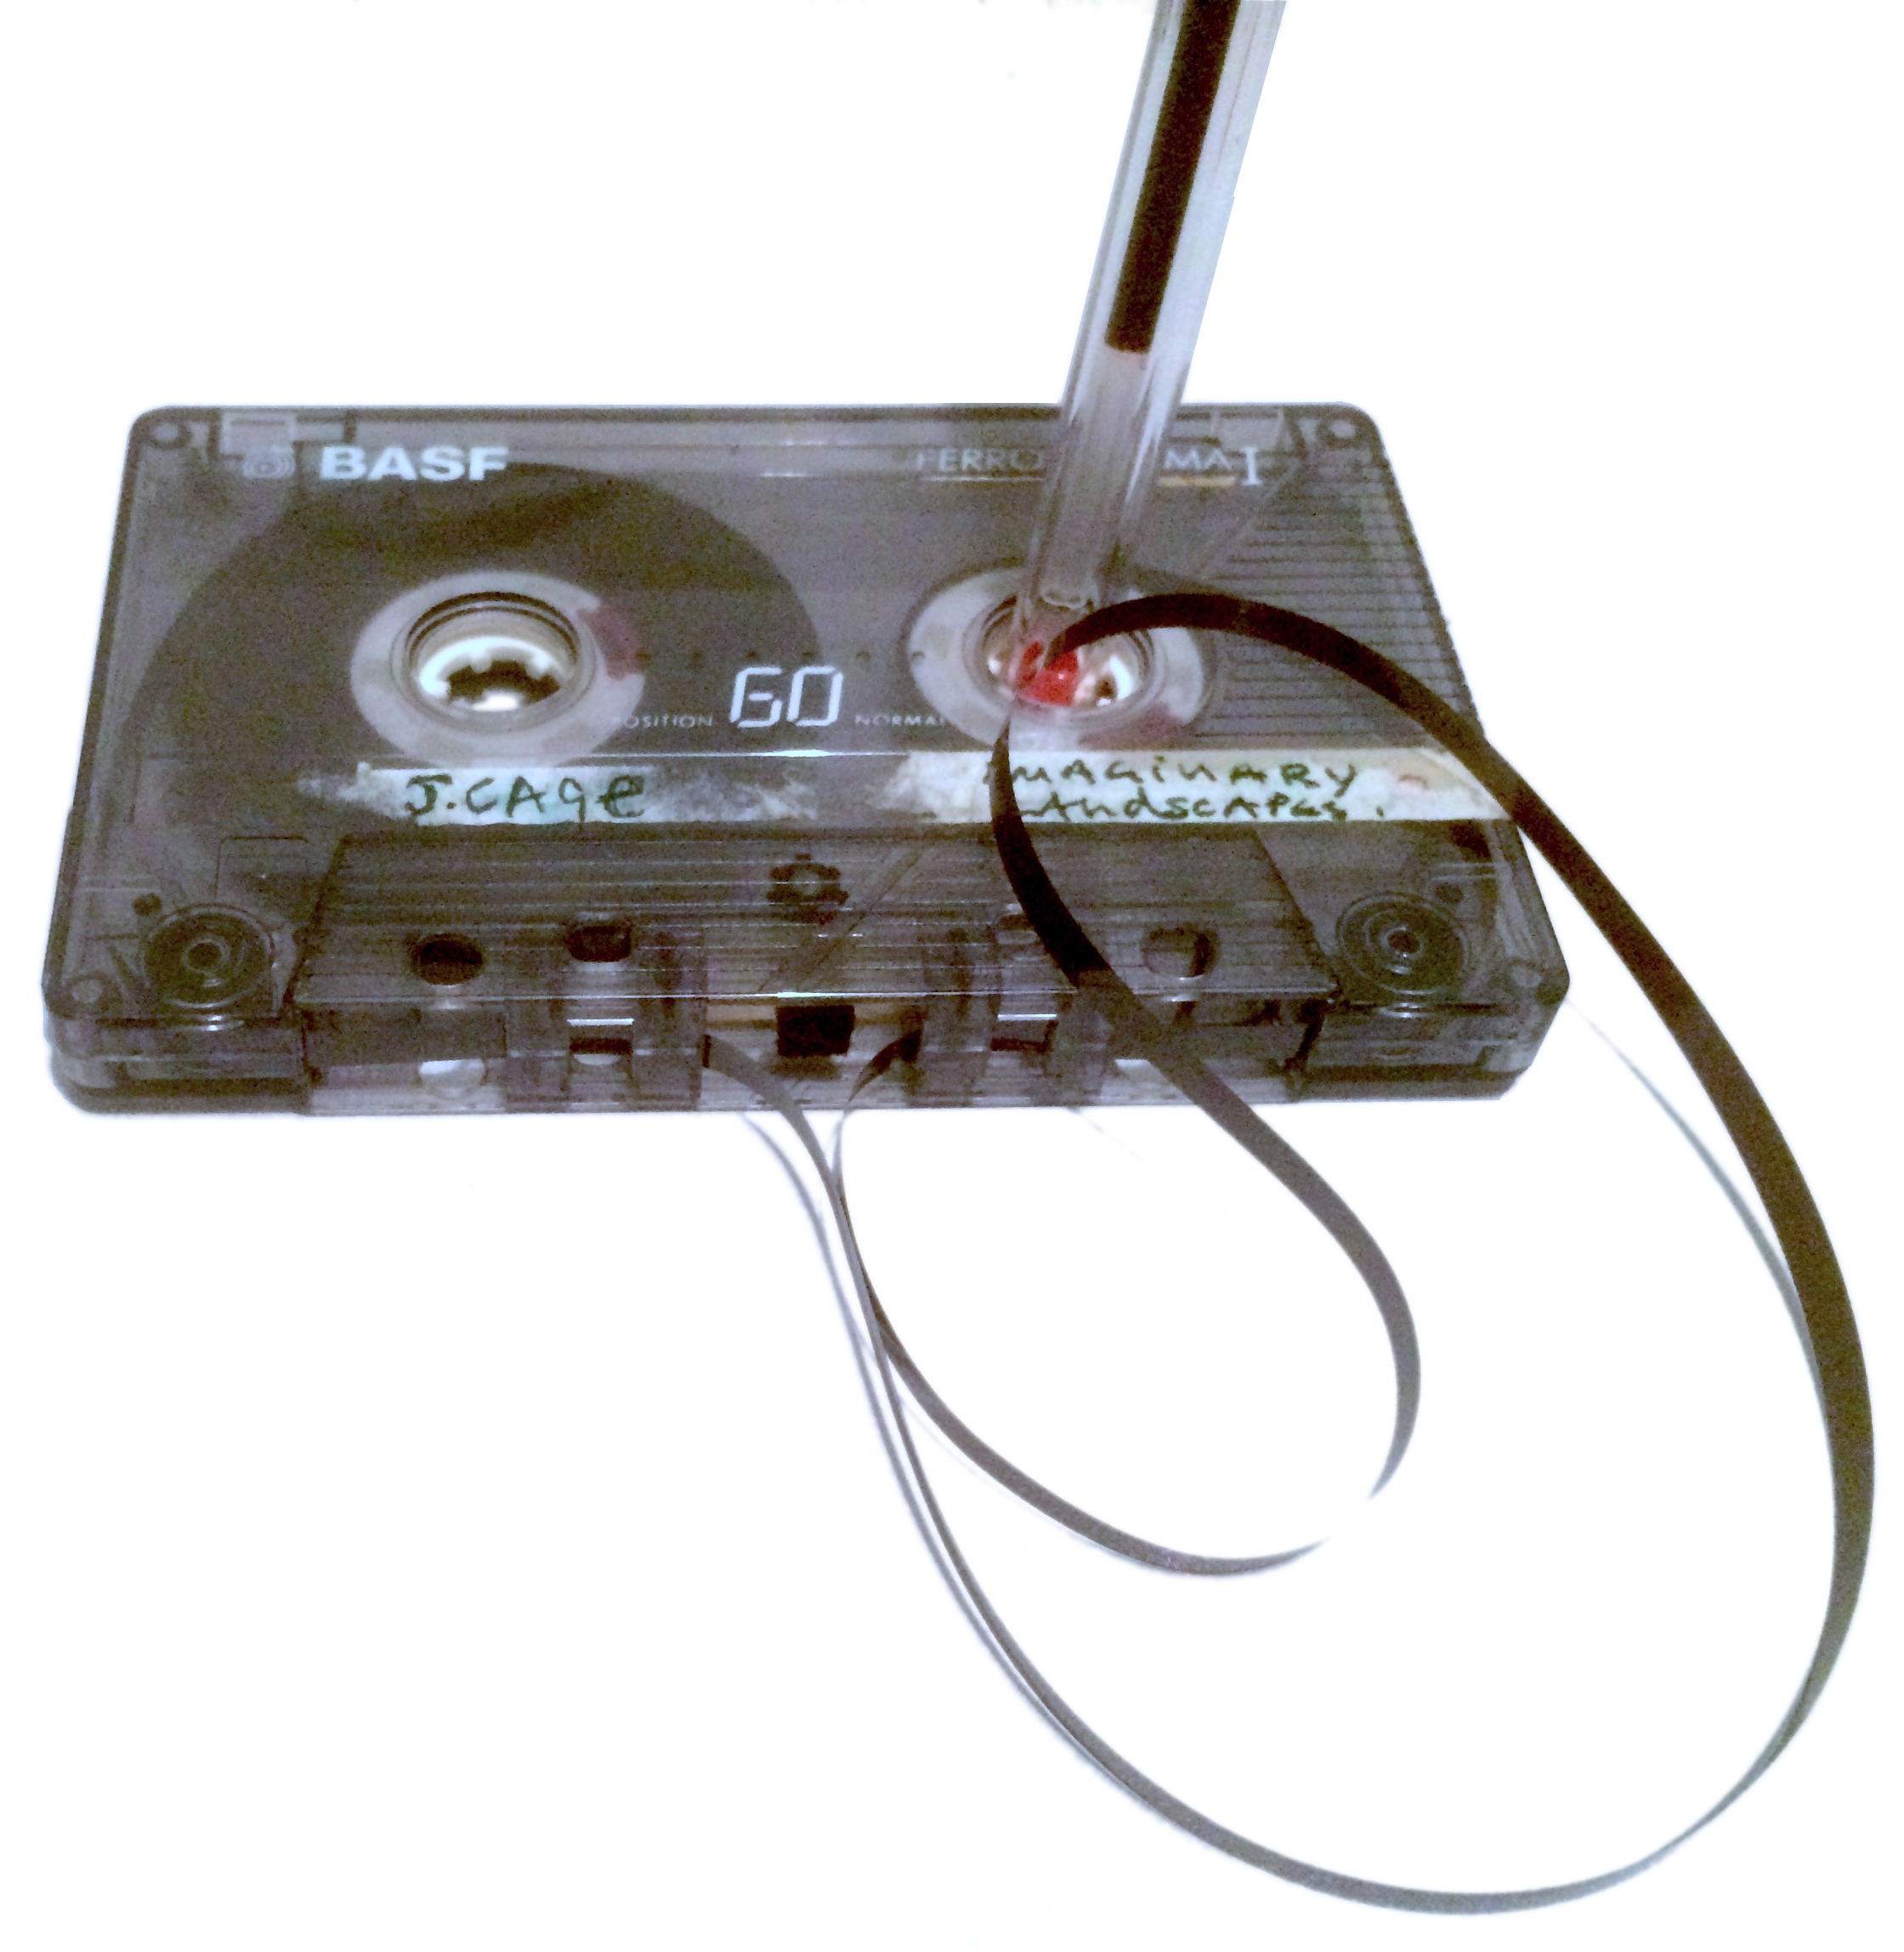
\includegraphics[width=0.56\textwidth]{gfx/01_preamble/K7.png}
 	%\vspace{-2em}
	%\caption[Walkman.]{Walkman.}
 	\label{fig:preamble:walkman}
\end{wrapfigure}
\par
\indent Aurais-je été en droit d'appeler mon balladeur-enregistreur un ``instrument'' ? Il n'existait aucun répertoire, aucune partition, aucun professeur enseignant sa pratique et en premier lieu, aucun musicien jouant d'un tel instrument en concert. Pourtant il y avait un public et je n'étais pas le seul auditeur; l'échange entre amis de compilations sur cassettes audio nous permettait de partager des morceaux, et à défaut d'en être les auteurs, nous étions les auteurs de nos sélections musicales.\\
\indent Une dizaine d'années plus tard, la dédicace que je lis à l'ouverture de l'imposant \textit{Traité des objets musicaux} de Pierre Schaeffer se fait l'écho : \iquote{À la mémoire de mon père, violoniste, dont je transmets le précepte : Travaille ton instrument}. 
Ce précepte qui prend la forme d'une injonction laisse imaginer la scène du père qui ordonne au petit Pierre d'aller faire ses gammes. Mais quel est donc l'instrument que Pierre Schaeffer semble avoir suffisamment travaillé pour reprendre ce précepte en ouverture de son ouvrage majeur ? Le disque à sillon fermé ? Le \textit{Phonogène} ? Où s'agirait-il davantage de sa propre perception auditive, dont il entreprend l'étude systématique pour en déchiffrer les ``modes de jeu'' ?

\indent Ce travail de recherche a commencé après plus de 15 années passées à concevoir, fabriquer, programmer, pratiquer et écouter des instruments de musique à l'aide d'ordinateurs. J'ai créé durant ces années diverses sortes d'applications, d'instruments, d'installations, d'outils, dans différents contextes : spectacle vivant, installations multimédia, ateliers pédagogiques, expositions muséographiques, émissions de radio, projets de recherche, etc. Il est sûrement vain de vouloir discriminer parmi tous ces objets lesquels constituent des instruments de musique et lesquels n'en sont pas, mais il me semble intéressant de constater que ces développements posent à chaque fois, sous différents angles, la question du rapport de musicalité avec la machine. C'est ce constat qui m'a amené à réfléchir sur ma pratique et sur la notion d'instrument de musique numérique pour essayer d'en cerner les contours, ou du moins, d'en percevoir les lignes de fuite.

\indent Poser la question de sa représentation, face à un medium numérique qui fait voler l’objet en éclat ainsi que les traditions musicales qu’il sous-tend, pose imanquablement celle des motivations pour lesquelles nous construisons des instruments, et par suite, des raisons pour lesquelles nous inventons, pratiquons, écoutons la musique. De cela découlent les multiples manières dont nous jouons avec le réel, avec les objets, avec les sons pour produire cet étrange --~et pourtant si familière~-- vibration de l'air.\\
\indent La notion d’instrument de musique numérique embrasse ces problématiques, complexes sur le plan technique, mais davantage encore sur le plan sociologique et esthétique. La façon dont nous créons la musique et la manière dont nous l’écoutons a tellement changé en un siècle qu’il semble désuet de tenter de l’aborder sur un plan purement technique, tant celle-ci semble promise à bouleverser encore davantage nos usages dans l’avenir. Le travail présenté dans cette thèse n'entend pas répondre à ces questions bien trop vastes mais tâchera, autant que possible, de ne pas perdre de vue les raisons profondes du désir musical, souvent difficile à expliquer et ranger dans des catégories et des articulations logiques.


\section{Une thèse interdisciplinaire}

sciences exactes + sciences humaines + pratique musicale

\noindent Cette thèse a été l'objet d'un contrat doctoral soutenu par le Collegium Musicæ, dont la mission est de promouvoir l'interdisciplinarité entre différents acteurs institutionnels œuvrant dans le champ de la musique. En l'occurence, cette thèse a été co-dirigée par Pierre Couprie, musicologue à l'\gls{IReMus} et Jean-Dominique Polack et Hugues Genevois, chercheurs de l'équipe \gls{LAM}. En se situant entre les domaines distincts des sciences et de l'ingénierie d'une part et de la musicologie d'autre part, cette thèse est la tentative d'une étude des \glspl{DMI} prenant ces deux dimensions en compte.

Par ailleurs, ce travail de recherche théorique est soutenu par des développements techniques disponibles librement sur Internet et dont j'espère qu'ils pourront profiter à la communauté des musiciens intéressés par ces outils.
Enfin, elle s'appuie sur des performances musicale mettant en œuvre ces développements pour confronter la théorie à la pratique tout autant que pour affiner la théorie sur la base de l'observation de ces pratiques. Elle constitue donc un travail de une recherche à la fois basée sur la pratique et dirigée par la pratique.


ajouer (éventuellement?) un mot sur les usages, formats et conférences relativement différentes et séparées dans ces domaines. 
Evolution vers une interdisciplinarité nécessaire à la compréhension mutuelle. Cf. présence d'article musicologie dans NIME.


\section{Qu'entend-on par ...}

\noindent Il s'agit ici de donner quelques éléments permettant de préciser la signification donnée à un certain nombre de termes dans ce document.

\subsection*{``Représentation...}

\noindent Le terme ``représentation'' recouvre un très vaste champ sémantique. Si son étymologie évoque le fait de ``rendre de nouveau présent'', la représentation passe aussi par l'image --~réelle ou mentale~--, distincte de l'originale représenté, que l'on se fait de quelque chose.

La question de la réprésentation (ou plutôt, des représentations) dans les lutheries numériques est envisagée sous différents angles, et présente ainsi des significations variables dans ce document : 
\vspace{-1em}
\begin{itemize}[noitemsep]
\item la représentation organologique des \glspl{DMI}, en particulier les manières variées dont il se présente comme agencements modulaires (ch. \ref{ch:ephemeral}) en contraste avec les représentations plus monolithiques de l'instrument classique;
\item la représentation de ce que l'on appelle communément ``le geste musical'' du point de vue des \glspl{DMI}(ch. \ref{ch:gesture});
\item la représentation physique du \gls{DMI} en tant qu'interface entre la continuité analogique du monde physique et l'espace discret de son inscription algorithmique, en particulier son aspect visuel dynamique lié à l'usage de l'infographie (ch. \ref{ch:interfaces});
\item la représentation proposée par le langage informatique dans lequel s'exprime le design de l'interaction musicale dans les \gls{DMI}, en particulier la manière dont s'articulent les messages venant représenter les données (gestuelles, audio, visuelles, etc.) à l'œuvre dans un \gls{DMI}, sous forme de signaux continus ou d'événements discrets (ch. \ref{ch:algorithms});
\item la représentation visuelle de l'interface de jeu, et en particulier son aspect dynamique lié à l'usage de l'infographie (ch. \ref{ch:visual_representation});
\item la représentation des éléments de vocabulaire musical dans le cas de l'improvisation électroacoustique jouée avec ces instruments numériques, en vue de leur notation (ch. \ref{ch:notation}).
\end{itemize}

\subsection*{...et contrôle...}

\noindent Le contrôle est éminemment lié à la question de la représentation, ce couple formant deux versants complémentaires --~action et perception~-- du phénomènes d'interaction. En l'occurence, si dans le cas des instruments acoustiques, on agit sur l'instrument dans le but de contrôler le son qu'il produit, on agit dans le cas des \gls{DMI} sur des représentations de sons et de gestes encodé sous la forme de données numériques. La question du geste instrumental y tient une place centrale et nous verrons notamment comment la causalité entre gestes et sons, se ré-articule dans le cas des \glspl{DMI}.

\subsection*{...dans le design interactif...}

\noindent Ces aspects de représentation et de contrôle sont ici étudiés dans la perspective concrète de leur prise en compte dans le travail de lutherie numérique. Le terme ``design interactif'' est un emprunt à l'anglais \iquote{interactive design}, généralement traduit par ``design de l'interaction'', c'est-à-dire la conception et la réalisation des fonctions qui assurent l'aspect interactif de l'objet que l'on conçoit. Cependant, sa version anglaise laisse entendre l'aspect interactif du processus de design lui même, ce qui reflète dans une grande mesure la manière dont le développement d'un \gls{DMI} (et des instruments de musique, de manière plus générale) se passe : dans un jeu permanent d'aller-retours entre la fabrication, la programmation, la pratique et l'écoute.

\subsection*{...des instruments...}

\noindent Une définition simple et efficace des instruments de musique serait la suivante : ``tout dispositif dont on se sert pour musiquer''. Cette définition qui peut apparaître comme un truisme présente l'intérêt de ne pas définir les instruments en fonction de leur nature ou de leur caractéristiques techniques, mais en fonction de leur usage. En particulier, l'utilisation du terme ``jouer'' vient préciser que, si de nombreux objets techniques permettent depuis le \siecle{20}siècle de ``produire'' de la musique à partir d'enregistrement, il ne sont envisageables en tant qu'\textit{instruments de musique} que s'ils sont joués, et non simplement ``utilisés''. Ainsi, la platine vinyle est un instrument de reproduction sonore quand elle est utilisée par le mélomane dans son salon, mais le même objet sera un instrument de musique s'il est joué.

On pourrait alors poser la question des contours que recouvrent le terme jouer.
Les instruments de musique ne sauraient donc être définis qu'à l'aune de la définition que l'on veut bien donner au terme musique. Une perspective intéressante du terme ``instrument'' cependant est sa double polarité d'objet qui sert à la fois à agir sur le monde (l'instrument-outil) et à le sentir (l'instrument de mesure).
Etymologie : \textit{struo} = construire, disposer, empiler, tramer.  \textit{instruo} : instruire, enseigner, former.

\iquote{Musiquer, c'est prendre part, quelqu'en soit notre capacité, à une performance musicale. Cela signifie non seulement jouer, mais aussi écouter, fournir des matériaux pour la performance --~ce que nous appelons composer~--, se préparer pour une performance --~ce que nous appelons répéter ou pratiquer~-- et tout autre activité connectée à la performance musicale. Nous devons certainement inclure le fait de danser, si quelqu'un danse, et nous pourrions même étendre la signification à l'occasion pour inclure ce que fait la dame qui prend les tickets à l'entrée, les gros bras qui déplacent le piano, ou les roadies qui préparent les instruments et portent le matériel de son, étant donné que leurs activités affectent également la nature de l'événement qu'est une performance musicale.}
\cite{small_musicking:_1998}

\Pierre{21-08 C'est super de parler de Small mais attention, tu mets un pied dans la sociologie et c'est bien dans ce périmètre qu'il conçoit le ‘musicking’. Je ne pense pas que cela corresponde à ce que tu nommes précédemment ‘musiquer’, ‘musicking’ est bien plus large.}

The digital has engendered a sense of novelty, curiosity, and originality in terms of performance, sound and music. The musical \textit{results} are strongly dependant on the instrument, and they often \textit{are} the instruments. Magnusson, Sonic Writing, p.61

Les instruments de musique sont des instrument pour jouer de la musique (ou pour musiquer, dirait Christopher Small \cite{small_musicking:_1998}). Cette apparente évidence est nécessaire pour signaler qu'il ne s'agit pas simplement de faire des notes, ou même du son. La musique implique également notre \textit{mémoire du son}, l'imagination que nous en avons, les aspects visuels qui se rattachent à la notion de musicalité, et d'autres dimensions esthétiques et culturelles. \todo{être plus précis}

La performance musicale a cela de particulier qu'elle ne possède pas de cahier des charges préalables (la partition ne saurait être considérée comme telle!) et que loin de se plier à la nécessité d'exécuter une tâche précise, comme il pourrait être le cas dans le design d'autres interfaces homme-machine, les instruments sont des objets techniques dont les musiciens abusent (plus qu'ils en usent), dont les artefacts peuvent être appréciables et souhaitables, dont la compréhension n'est pas un préalable requis pour leur utilisation, pas davantage que leur fiabilité n'est garante d'une performance musicale intéressante.

\Pierre{21-08 Ce paragraphe est une excellente definition de l'instrument numérique. C'est vraiment très bien dit.}

%
Le design des \glspl{DMI}, ainsi que le design des outils-mêmes du luthier numérique, doivent être informés de ces particularités propres à la création artistique si l'on souhaite qu'ils se prêtent à la création de musiques nouvelles et à l'exploration de territoires sonores inexplorés.


\subsection*{...de musique...} 
\subsubsection*{définition intrinsèque}
La musique est un concept difficile à définir et comme le dit le musicologue Pierre Billard en intoduction de la définition donnée par l'encyclopédie Universalis \iquote{plus notre connaissance de la musique est étendue et moins nous savons, en fin de compte, ce qu'elle est.}

Définir la musique sur la base de son contenu est probablement la perspective la moins consensuelle qui soit et dont l'intérêt principal est peut-être qu'elle qualifie surtout l'opinion de celui (ou du groupe) qui la définit ainsi : musique de son purs, musique de bruits, sons organisés de Varèse.
\subsubsection*{définition intrinsèque}

On peut définir la musique du point de vue de celui qui la produit (compositeur, instrumentiste) : « Tout corps sonore utilisé par le compositeur est un instrument de musique. » Berlioz, 1843, Grand Traité d'instrumentation et d'orchestration modernes

Définir la musique du point de vue de celui qui l'écoute : est musique tout ce que j'écoute et considère comme telle.

La musique est un art de la résonance, qu'elle soit d'ordre acoustique et physique, ou d'ordre plus intellectuelle et spirituelle. La musique fait écho.

\subsection*{...numériques}

\indent On parle souvent, par métonymie, des ``musiques électroniques'' ou ``musiques numériques'' pour désigner des productions musicales où l'empreinte de ces medias caractérise de manière prononcée une certaine esthétique. Mais le terme ``numériques'', dans le titre de cette thèse, est au pluriel car c'est bien le caractère numérique des instruments auquel je m'intéresse dans ce travail et ses conséquences en terme de lutherie. Ces specificités seront analysées plus en détail dans la perspective propre à chaque chapitres, mais j'en évoquerai ici les traits principaux :
\vspace{-1em}
\begin{itemize}[noitemsep]
\item \textbf{le découplage énergétique} : introduit par l'utilisation de l'électricité;
\item \textbf{le représentation symbolique} : qui permet de manière générale l'enregistrement et l'agencement sur un medium commun de données aussi diverses que des échantillons sonores, des algorithmes ou des structures de représentation de données;
\item \textbf{les capacités de stockage en mémoire} : qui permettent notamment le temps différé (davantage que le ``temps réel'') et l'élaboration d'écritures dynamiques 
\item \textbf{la computation} : le traitement algorithmique qui permet --~ou impose~-- une reconfiguration permanente des modèles et des représentations;
\item \textbf{le réseau} l'inscription des \glspl{DMI} dans l'écosystème du numérique, qui permet la distribution, l'échange, la mise en commun, la duplication des ressources sur des modules et plateformes en réseau.
\end{itemize}

J'utiliserai parfois le terme de ``musicien numérique'' au sens où le définit Andrew Hugill comme \iquote{quelqu'un qui a saisi les possibilités ouvertes par les nouvelles technologies, en particulier le potentiel de l'ordinateur pour explorer, stocker, manipuler et traiter le son, ainsi que le développement de nombreux autres outils et dispositifs numériques qui permettent l'invention et la découverte musicale}\footnote{Dans son ouvrage \textit{The Digital Musician} \cite{hugill_digital_2019}}.

C'est ici ce qu'amène le numérique qui m'intéresse, c'est-à-dire ( TODO) l'utilisation d'une forme symbolique automatisée et traitable en grande quantité par les ordinateurs. Ce que cela apporte aux instruments, ce qui unit ou sépare les différents types d'instruments numériques ensemble et par rapport aux lutheries classiques.


\section{Problématique}

\noindent La conception des \glspl{DMI} rassemble des questions qui étaient relativement dissociées dans la lutherie acoustique traditionnelle : les rôles du facteur d'instrument, du compositeur, de l'interprète et de l'auditeur y sont généralement assumés par des personnes distinctes. Les nouvelles lutheries, et particulièrement celles usant de technologies numériques, redistribuent ces fonctions qui bien souvent se retrouvent endossées par une même personne. En particulier, la possibilité de modéliser les savoirs-faire propres à ces différents domaines dans des outils qui prennent en charge tout ou partie de leur mise en œuvre permet de nuancer la part d'implication du \textit{musicien numérique} dans chacun de ces domaines d'expertise.

\indent La question centrale de cette thèse sera donc formulée ainsi : comment, dans cette redéfinition généralisée des interactions entre le geste et le son, le réel et le virtuel, l'écriture et l'interprétation, s'articule l'agencement d'un \gls{DMI} ?

le musicien, son instrument, face auquels s'ouvre un infini des possibles sonores, s'articulent l'agencement d'un \gls{DMI} et l'agentivité relative ?

\Pierre{ Je ne vois pas de problématique présentée. La problématique est la question que tu poses dans ta thèse ainsi que les questions annexes ou sous-questions.}

Nécessité de prendre en compte la part expérientielle de la performance musicale, notamment dans sa dimension subversive.

Cette thèse propose une étude de la création et la performance musicale avec des \gls{DMI}, pour essayer d'en re-définir les contours et en tirer des conséquences sur leur design.

Notamment, en envisageant le geste musical comme phénomène dépassant l'approche fonctionnelle qui lui est souvent conférée dans les études en \gls{IHM}, et en analysant les \glspl{DMI} en tant qu'assemblages et processus possédant des qualités propres et différentes de celles des instruments acoustiques, ce travail vise à étudier comment les différents enjeux qui se posent avec de tels instruments dans la performance musicale s'articulent au niveau de leur conception.

Quelques questions : 
\vspace{-1em}
\begin{itemize}[noitemsep]
\item Au delà des métaphores de la bureautique (menus, sliders, checkbox), quel vocabulaire graphique est envisageable pour le design des éléments d'interaction ?
\item Comment gérer les scénarios de déconnexion / reconnexion dynamiques intervenant dans le cours d'une performance ?
\item Comment noter la musique (électroacoustique) produite avec de telles interfaces pour le jeu collectif ?
\item Quelles interfaces seront pertinentes lors des différentes phases de conception, de composition, de répétition, ou de performance avec l'instrument ?
\item  Quelles représentations privilégieront, pour le contrôle de paramètres identiques, tantôt la virtuosité, la précision, l'étendue de de la palette sonore, la polyphonie gestuelle ou encore la structure temporelle ?
\end{itemize}

\section{Enjeux et hypothèses}

Enjeu de trouver des caractéristiques transversales dans les lutheries numériques malgré l'absence de tradition, de répertoire, de notation, de méthode d'apprentissage, etc.
Enjeu de confronter au réel des réalisations instrumentales et logicielles à travers une pratique musicale.

Ce travail tente de présenter l'ensemble d'une démarche de création d'un \gls{DMI}, comprenant sa conception, sa fabrication, sa programmation, sa pratique, et la composition avec cet instrument.
Ce travail de recherche s'offre donc comme une présentation ``en coupe'' d'un travail de lutherie, dans ce qu'il comporte de réflexions, de choix de matériaux, d'assemblages, de programmation, de notations, de pratiques et comment ces différents aspects interfèrent dans le cas particulier des instruments intégrant le numérique dans le design de leur interaction.

\subsubsection*{Hypothèse 1 : l'instrument atomisé, recomposé}

L'instrument est atomisé et se retrouve configuré comme un agencement modulaire évolutif qui se cristallise ponctuellement dans des instances contextuelles. \\
Pas d'instrument standard qui sorte du lot, si ce n'est pour imiter l'existant (le clavier, la guitare, etc.), mais des protocoles et modules qui deviennent standards et interconnectables.

\subsubsection*{Hypothèse 2 : l'instrument est subversif}

\Pierre{ le subversif est une très bonne idée mais c'est un terme tellement chargé de sens que tu dois en dire un peu plus et notamment dans quel sens tu le prends.}

La relation instrumentale n'est pas de même nature que la relation des HCI.
Les instrumentistes ne sont pas des \textit{interface users} mais plutôt des \textit{interface abusers}.
La relation entre le geste et le son n'est pas nécessairement faite pour être lisible et comprise du public, le musicien est un magicien.
L'œil augmente l'écoute (et la subvertit).


\subsubsection*{Hypothèse 3 : Le continu et le discret}

Si la continuité de la vibration physique semble être une donnée consitutive des instruments acoustique, qui recrééent artificiellement des espaces discrets (tels que les échelles harmoniques et rythmiques), le domaine du numérique part d'une certaine manière dans la direction opposée. Les instruments numériques sont caractérisé par la nature discrète (et même binaire) de l'encodage symbolique sous-jacent aux données traitées. Il s'agit donc davantage de pouvoir retrouver une continuité dans ce monde discret.\\
Cette bipolarité du continu et du discret traverse ainsi, à des degrés variés, les questions de design qui se présentent dans la conception des instruments numériques, que cela soit au niveau de l'encodage du geste capté ou de celui de la synthèse audio. Les développements présentés dans ce travail sont orientés par les possibilités de passage fluide du continu au discret et inversement, animés par la conviction qu'une partie du jeu musical se joue dans cette ambivalence, en soutenant l'aspect suversif du geste musical.


\section{Interviews}

Une caractéristique notable des lutheries numériques est leur diversité et le foisonnement d'approches, de propositions, de positions prises par ceux qui les inventent et les pratiquent. Un certain nombre d'entretiens ont été menées durant ce travail de thèse afin d'élargir le champ de la réflexion à différentes approches sur les \glspl{DMI}. Ces entretiens sont reproduits intégralement en annexe, accompagnés d'une brève biographie présentant les personnes ayant acceptés de présenter leur travail et leurs réflexions.

Ces interviews ont pris la forme de discussions libres, orientées par un certain nombre de questions, dont la première était invariablement : quelle a été la motivation originale qui vous a poussé à concevoir et utiliser des DMI ?. La suite de la discussion dépendait ensuite de l'interlocuteur, leurs projets étant relativement différents entre ceux d'entrepreneurs et ceux d'artistes. %On y trouve cependant quelques idées transversales qui ont contribuées à nourrir ma propre réflexion.

\todo{reproduire le guide d'interview en annexe}

Liste des personnes interviwées (et liens vers annexes) :

\vspace{-1em}
\begin{itemize}[noitemsep]
\item \textbf{\hyperref[appendix:bernier]{Nicolas Bernier}}, artiste canadien créant des installations et performances audio-visuelles, et enseigne la "musique numérique" à l'Université de Montréal;
\item \textbf{\hyperref[appendix:collins]{Nicolas Collins}}, compositeur, artiste sonore, professor au département son  à la School of the Art Institute de Chicago 1999 et auteur notable du livre "Handmade Electronic Music –The Art of Hardware Hacking";
\item \textbf{\hyperref[appendix:dumeaux]{François Dumeaux}}, musicien et compositeur de musiques électro-acoustiques;
\item \textbf{\hyperref[appendix:delaubier]{Serge De Laubier}}, musicien, inventeur du Méta-Instrument, directeur artistique de Puce Muse;
\item \textbf{\hyperref[appendix:fernandez]{Jose-Miguel Fernandez}}, compositeur 
%\item \textbf{\hyperref[appendix:kurtag]{György Kurtag Jr.}}, musicien improvisateur, compositeur, pédagogue...
\item \textbf{\hyperref[appendix:mamou-mani]{Adrien Mamou-Mani}}, chercheur et co-fondateur de HyVibes, startup créant des instruments augmentés tels la \textit{SmartGuitar};
\item \textbf{\hyperref[appendix:saint-denis]{Patrick Saint-Denis}}, compositeur, luthier numérique, enseigne à l'Université de Montréal.
\item \textbf{\hyperref[appendix:turchet]{Lucas Turchet}} (b. 1982), designer sonore, musicien, compositeur et écrivain, co-fondateur de Mind Music Labs, startup créant des instruments augmentés.
\item \textbf{\hyperref[appendix:zamborlin]{Bruno Zamborlin}} (b. 1984), fondateur et CEO de Mogees et HyperSurfaces. 
\end{itemize}



\section{Contributions de cette thèse}

Cette thèse propose plusieurs contributions théoriques dans le domaine de la recherche sur les \glspl{DMI}, ainsi que plusieurs contributions pratiques sous la forme de \glspl{LogicielLibre} et disponibles sur le web.

Les contributions théoriques concernent :
\vspace{-1em}
\begin{itemize}[noitemsep]
\item des perspectives sur la nature des \gls{DMI}, leur cycle de vie, la notion d'assemblage éphémère et ses conséquences sur leur design et leur pratique (dans le chapitre \ref{ch:ephemeral});
\item la caractérisation du geste musicale, en particulier la proposition d'une nomenclature qui s'émancipe du modèle instrumental acoustique;
\item la mise en perspective de cette typologie gestuelle avec des stratégies d'interaction intégrant la part subversive de la performance musicale et son inscription dans le design de l'instrument (dans le chapitre \ref{ch:gesture});
\end{itemize}

Les contributions pratiques sont les suivantes :
\vspace{-1em}
\begin{itemize}[noitemsep]
%\setlength\itemsep{-1.5em}
\item \textbf{LAM-lib} : un package pour le logiciel Max proposant une collection d'algorithmes utiles pour la lutherie numérique;
\item \textbf{MP} : un protocole de communication pour le contrôle de la synthèse, venant palier un certain nombre de limitations rencontrées dans le protocole MIDI, ainsi qu'un package Max rassemblant un certain nombre d'objets supportant ce protocole;
\item \textbf{mp.TUI} : un package pour Max permettant la création d'interfaces graphique tangibles personnalisables et polyphoniques, basées sur le protocole MP;
\item \textbf{sagrada} : un package Max de synthèse granulaire modulaire contrôlé par signal;
\item \textbf{John} : un logiciel pour la (semi-) composition et conduite d'improvisation électroacoustique, éditable collectivement;
\end{itemize}


\section{Structure de la thèse}
\label{sec:preamble:structure}

\textbf{Chapitre \ref{ch:introduction}} \\[0.2em]
Vous êtes ici.

\textbf{Chapitre \ref{ch:ephemeral}} \\[0.2em]
Le chapitre \ref{ch:ephemeral} présente un certain nombre de considérations sur les \glspl{DMI} et le contexte de leur utilisation. En particulier, la nature éphémère des assemblages modulaires, souvent ignorée, est ici considérée comme une des caractéristiques essentielles venant influencer leur design. Un distribution entre répertoire, musicien et contexte permet de re-définir la façon dont s'articulent ces différents pôles ainsi à l'œuvre dans la création et l'évolution des DMIs.

\textbf{Chapitre \ref{ch:gesture}} \\[0.2em]
Le chapitre \ref{ch:gesture} vient questionner la notion de geste musical dans le cas de la pratique avec des DMIs. En particulier, la lisibilité du geste et de sa relation à la synthèse sonore, souvent considérée comme un critère de design souhaitable, y est remise en question en prenant en compte les fins subversives de l'art musical. 

L'étude des artefacts qui en résultent et viennent bouleverser la perception de continuité(s) permet d'introduire la notion de morpho-dynamisme des DMIs, son intérêt dans la création et la pratique musicale et son intégration dans le corps de l'instrument.

\textbf{Chapitre \ref{ch:interfaces}} \\[0.2em]
Le chapitre \ref{ch:interfaces} présente une exemple particulier d'interface instrumentale et retrace l'histoire de son évolution à travers plusieurs générations, partant d'une interface standard et disponible dans le commerce (la tablette graphique) et évoluant vers une personnalisation et un enrichissement du dispositif. 
Seront discutées les raisons motivant l'ajout de capteurs, l'organisation de l'espace de jeu, la polyphonie des sources sonores, etc.

\textbf{Chapitre \ref{ch:algorithms}} \\[0.2em]
Le chapitre \ref{ch:algorithms} présente des développement réalisés pour la conception du ``mapping'' de l'instrument en tentant notamment de répondre aux problématiques soulevées dans les chapitres \ref{ch:ephemeral} et \ref{ch:gesture}. Sont présentés dans ce chapitre les concepts de modèle intermédiaire, ainsi qu'un protocole de contrôle expressif polyphonique, nommé ``MP'', permettant la communication entre interfaces, modules de transformation et de synthèse. Une extension des idées de MP dans le domaine du signal et appliqué à la synthèse granulaire, nommé Sagrada, est également présenté.

\textbf{Chapitre \ref{ch:visual_representation}} \\[0.2em]
Le chapitre \ref{ch:visual_representation} présente un système d'interface graphique tangible (TUI) basée sur le protocole présenté au chapitre  \ref{ch:algorithms}, afin de permettre notamment une reconfiguration dynamique de l'interface de jeu et une représentation graphique des processus utilisés pour la performance musicale. Ces interfaces graphiques permettent également d'intégrer des éléments de représentation musicale (forme d'onde, échelle, motifs rythmiques, etc.) ou non-musicale comme composants interactifs pour le contrôle expressif.

\textbf{Chapitre \ref{ch:notation}} \\[0.2em]
Le chapitre \ref{ch:notation} présente des travaux portant sur la notation musicale dans le domaine de la performance électroacoustique utilisant des DMI. Les questions de composition collective, d'édition collaborative et d'écologie de l'attention sont abordées et sont mises en œuvre dans ``John, the semi-conductor'', un logiciel permettant la génération automatique et l'édition collective de partitions minimales, utilisé dans l'ensemble d'improvisation électroacoustique ONE. 

\textbf{Chapitre \ref{ch:conclusion}} \\[0.2em]
Pistes de recherches à suivre...


\section*{extra material}
 % INCLUDE: preamble
% !TEX root = ../thesis-example.tex
%
\chapter{Instances éphémères d'agencements modulaires}
\label{ch:ephemeral}

% \cleanchapterquote{Paradoxalement, la musique du futur est écrite sur du sable!}{Michel Chion}{La musique du futur a-t-elle un avenir?, 1977}

%\cleanchapterquote{Le vieux Paris n'est plus (la forme d'une ville\\
%Change plus vite, hélas ! que le coeur d'un mortel)}{Charles Baudelaire}{Le Cygne, 1861}

\cleanchapterquote{La musique (...) est trop en deçà du monde\\
et du désignable pour figurer autre chose\\
que des épures de l'Être, son flux et son reflux,\\
sa croissance, ses éclatements, ses tourbillons.}
{Maurice Merleau-Pontry}{L'Œil et l'Esprit, 1964} %\cite{merleau-ponty_loeil_1964}

%\cleanchapterquote{Dufourt suggests that contemporary music\\
%highlights what was rejected in the Greek world:\\
%it rather captures the evanescent, the ephemeral,\\
%the ambivalent, the Erebus, it favors the endless\\
%metamorphosis of qualities and forms;\\
%as Nietzsche proclaimed, western music tends\\
%toward the liberation of the dyonisiac dimension\\
%and the acceptance of the inacceptable part of myths.}
%{Jean-Claude Risset}{Discours invité à la conférence ICMC, 2014}%\cite{risset_sound_2014} % Remettre cette citation dans le corps du texte.

\vspace*{\fill}

\noindent Nous avons exposé dans le préambule le fait que l'instrument de musique ne se laisse pas facilement définir, tant la notion de musique est sujette à des interprétations diverses, et que l'apport du numérique sembler venir brouiller davantage encore les définitions et contours de l'objet. L'expression \textit{digital musical instrument}, dont l'usage croissant depuis le tournant du millénaire a fini par la condenser en l'acronyme ``\gls{DMI}'', pourrait nous laisser croire, a contrario, qu'une forme certes mal-définie se cristallise. Pourtant, il semble que ce soit l'\textit{éphémérité}, ou l'\textit{obsolescence} des \glspl{DMI} (selon la perspective optimiste ou pessimiste que l'on adopte) qui les caractérisent, davantage qu'une stabilité effective, et qui se traduit par un souci croissant de la question de leur pérennité.\\
\indent Après un rapide historique de l'émergence des \gls{DMI}, j'analyserai dans ce chapitre les termes de leur instabilité, dans la perspective de ce qu'ils impliquent comme choix et méthodes adaptés pour la conception et la pratique.

\clearpage

%\test{blabla}
\section{Paysage des DMIs}
\label{sec:ephemerality:landscape}

%--------------------------------------------------------------
\subsection{Les origines}
\label{sec:ephemeral:origins}

\subsubsection{Pré-histoire}
\label{sec:ephemeral:origins:prehistory}

\noindent Les instruments acoustiques héritent d'une histoire vieille de plus de 40~000 ans \cite{conard_new_2009} et la finesse de leur fabrication a atteint une excellence qui fait de certains instruments de véritables pièces d'orfèvres. Les instruments numériques, beaucoup plus récents en comparaison, ne peuvent rivaliser avec ce degré de raffinement. Pour autant, il ne sont pas totalement déshérités de la tradition et du savoir-faire des instruments acoustiques et, par ailleurs, le développement hautement collaboratif à l'œuvre dans le domaine de la programmation informatique leur confère, malgré leur jeunesse, une grande complexité — les compétences requises pour la fabrication d'un \gls{DMI} de A à Z dépassant souvent largement ce qu'il serait possible pour un individu seul de concevoir. C'est en effet un trait caractéristique des objets techniques de l'ère post-industrielle que d'être le produit du travail d'un très grand nombre d'individus\footnote{Un exemple notoire en fut donné par l'économiste Leonard Read (et repris par Milton Friedman) dans l'essai ``I, pencil''\cite{read_i_1958}, prenant l'exemple d'un simple crayon à papier pour démontrer que des millions de gens avait collaboré à sa fabrication.} et d'être assemblés à partir d'éléments de base déjà manufacturés et complexes.\\
\indent Parmi les diverses caractéristiques des \glspl{DMI}, la plus notable est probablement le découplage total entre le geste du musicien et le son. Ce découplage énergétique et plus généralement, l'extériorisation du travail dans les outils, est un processus ancien qui a été en particulier analysé par le paléo-anthropologue André Leroi-Gourhan \cite{leroi-gourhan_geste_1964}. En ce qui concerne les instruments, on observe des ruptures dans l'histoire de la lutherie au moment de grandes avancées scientifiques et technologique. Jean-Claude Risset\index[people]{risset@Risset, Jean-Claude} note en particulier dans \cite{genevois_les_1999} la naissance de l'orgue comme un moment charnière, au regard des questions qui m'intéressent ici: \iquote{L'orgue marque le rôle croissant de la technologie dans l'instrument de musique: il introduit le premier interrupteur, le premier clavier, et dès le \siecle{15}~siècle la première synthèse additive (qui ne sera justifiée mathématiquement par Fourier qu'au \siecle{19}~siècle). L'orgue est aussi la première machine informationnelle: l'information donnée par le geste du musicien y est décuplée de l'énergie sonore.}\footnote{On notera au passage que le terme ``décuplé'', qui semble être une coquille (intentionnelle ?) du terme ``découplé'', reste tout à fait pertinent!}\\
\indent La révolution industrielle est un autre moment charnière, une période de nombreux développements qui anticipent les révolutions technologiques du \siecle{20}~siècle. On notera notamment les progrès mécaniques: les machines-outils permettent la réalisation de pièces mécaniques de plus en plus précises et fabriquées en grande série. Cela donnera lieu notamment à des systèmes tels que le clétage de Boehm, qui permet le déport des doigts et révolutionne la famille des instruments à vent. Enfin (et surtout), l'arrivée concomitante de la téléphonie et de l'enregistrement dans la seconde moitié du \siecle{19}~siècle, qui déportent la production sonore dans l'espace et dans le temps et seront les vecteurs d'une transformation profonde de la société, et en particulier pour ce qui nous intéresse ici, des modes de production et de réception de la musique\footnote{Sur ce vaste sujet, voir en particulier~\cite{theberge_any_1997}.}.

%Introduction de la mécanique, déport du doigté (Boehm) — révolution industrielle\\
%Introduction de l'électricité (théremin, Martenot, patching de la téléphonie)\\
%Introduction de l'enregistrement (phonographie, bande, Schaeffer et l'écoute réduite)\\

\subsubsection{L'arrivée du numérique}

\noindent Si les premières productions musicales par ordinateur datent du début des années 1950\footnote{Elles sont attribuées à Geoff Hill\index[people]{hill@Hill, Geoff} sur l'ordinateur ``CSIRAC'' à Sydney, Australie, et à Christopher Strachey\index[people]{strachey@Strachey, Christopher} sur le ``Ferranti Mark 1'' à Manchester, Royaume-Uni, toutes deux en 1951. Des enregistrements restaurés de la musique de Strachey sont accessibles en ligne: \\ \url{https://soundcloud.com/guardianaustralia/first-ever-recording-of-computer-music} et celle de Hill a été reconstruite par Paul Doornbusch, voir \cite{doornbusch_computer_2004}.}, c'est à Max Mathews, qu'on attribue généralement la paternité de la musique sur ordinateur, en tant qu'auteur du langage Music I en 1957 et de la famille de programmes qui suivront, connue sous le nom générique ``Music-N''.\\
\indent Après de nombreuses productions musicales sur synthétiseurs analogiques dans les années 1960, arrivent les premiers développements numériques temps-réel. Au début, la bande passante de l'électronique numérique ne permet pas encore la synthèse audio temps-réel, mais est suffisante pour numériser des signaux de plus basses fréquences tels que ceux issus de boutons et potentiomètres. Les années 1970, époque du ``mini-ordinateurs'', donnent ainsi naissance à des systèmes hybrides permettant un contrôle numérique (et l'utilisation d'algorithmes), tandis que la synthèse sonore est assuré par des oscillateurs analogiques. C'est le cas par exemple dans le système GROOVE\footnote{``\textit{Generated Realtime Operations On Voltage-controlled Equipment}''} développé en 1967 par Max Mathews\index[people]{mathews@Mathews, Max} et Richard Moore aux laboratoires Bells, du CEMS\footnote{``\textit{Coordinated Electronic Music Studio}''} conçu par Joel Chadabe et construit par Robert Moog en 1967, ou encore de la \textit{Sal-Mar Construction} créée par Salvatore Martirano\index[people]{martirano@Martirano, Salvatore} et ses étudiants entre 1969 et 1971 à l'Université d'Illinois.\\
\indent Durant les années 1970, l'arrivée sur le marché de nouvelles cartes électroniques à accès rapide stimule le développement des stations de calcul audio temps-réel. En France, plusieurs projets de systèmes temps-réels sont lancés simultanément par plusieurs centres de création : à l'\gls{IRCAM} Giuseppe Di Giugno développe la série de \gls{DSP} temps-réel 4A (en 1976), 4B (en 1977), 4C (en 1978), 4X (en 1981), au \gls{CEMAMu} Iannis Xénakis invente l'\gls{UPIC} en 1977, tandis que Jean-François Allouis développe le système Syter \cite{teruggi_technology_2007} au \gls{GRM} en 1977. Il est intéressant de noter comment ces différents systèmes de synthèse sonore \gls{DSP}, créés durant les mêmes années, se distinguent déjà fortement, en étant marqués par la philosophie et l'esthétique musicale de leur maison de création : l'influence de l'architecture chez Xénakis\index[people]{xenakis@Xénakis, Iannis}\footnote{L'interface de l'\gls{UPIC} est une tablette graphique d'architecte.}, le contrôle total de la synthèse chez Boulez\index[people]{boulez@Boulez, Pierre}\footnote{Voir notamment les propos de Boulez dans \cite{albera_pli_2017} reflétant cette obsession pour le contrôle absolu.}, le traitement ``plastique'' du son au \gls{GRM}. Outre ces stations de calcul ``\textit{mainframe}''\footnote{On appelle ``\textit{mainframe}'' les ordinateurs centraux, de grande puissance et généralement de grande taille, dédiés au calcul spécialisé dans les grandes entreprises et les laboratoires de recherche.}, c'est aussi le début de la commercialisation de synthétiseurs numériques, à des prix plus abordables que leurs prédécesseurs analogiques: le Casio VL-1 (1979), l'E-mu Emulator (1982), le Yamaha DX7 (1983), ainsi que la norme \gls{MIDI} (1983) en sont les exemples les plus significatifs.\\
\indent Parallèlement à l'\gls{IRCAM}, Miller Puckette développe ``The Patcher'' (1985), ancêtre de Max. En 1989, la station \gls{ISPW}/\gls{FTS}, d'abord pilotée par Max, puis intégrée dans Max, annonce l'arrivée de la synthèse audio programmable en temps-réel sur les ordinateurs grand public et, par suite, de la démocratisation\footnote{Démocratisation relative toutefois, car si elle sort des institutions pour trouver sa place auprès d'un plus large public, elle est avant tout présente dans les pays dits ``développés'', ce qui à l'époque représente essentiellement les pays d'Europe de l'Ouest, d'Amérique du Nord, l'Australie, la Nouvelle-Zélande et le Japon.} des lutheries numériques.


\subsection{Différents types de DMIs}

\noindent Depuis lors, les \glspl{DMI} se sont multipliés en des formes hybrides qui germent à la croisée des arts et des pratiques. Je mentionne ci-après quelques directions, en explicitant ce qui les caractérise, mais ces différents axes de développement ne pourraient être tenus pour des catégories étanches.

%--------------------------------------------------------------
\subsubsection{Contrôleurs et synthétiseurs MIDI}

\noindent Les instruments \gls{MIDI} sont généralement séparés en deux parties : un ``contrôleur'' d'une part, uniquement destiné à la captation du geste, et un synthétiseur d'autre part, uniquement destiné à la production du son. Ces instruments sont apparus à partir des années 1980 avec l'arrivée du standard \gls{MIDI} qui permet la communication entre ces deux parties, lui-même inspiré directement du clavier de piano. De manière générale, les interfaces \gls{MIDI} se résumaient à des claviers et des pads de percussion, c'est-à-dire des instruments à touches de déclenchement, avec une sensibilité plus ou moins fine à la vélocité de déclenchement et à la pression sur la touche.\\
\indent On peut toutefois distinguer deux générations depuis l'arrivée du \gls{MPE} en 2018\footnote{La reconnaissance officielle par la \gls{MMA} date de début 2018, mais des instruments existaient déjà depuis 2014.}, et des interfaces dites ``expressives''\footnote{On peut par exemple citer le Seaboard de Roli, le Linnstrument de Roger Linn ou encore le SoundPlane de Madrona Labs.} permettant une modulation indépendante par note.\\
\indent En dehors de cet usage conforme au standard, le protocole \gls{MIDI} a également souvent été détourné pour contrôler des synthétiseurs de manière plus expérimentale. Ce détournement est à la fois lié aux limitations du \gls{MIDI} en regard des possibilités d'expression sonore permises par l'audio-numérique, mais avant tout, en raison de son omniprésence hégémonique sur les outils technologiques audio.

%--------------------------------------------------------------
\subsubsection{Instruments augmentés}

\noindent Les instruments augmentés sont caractérisés par un design dont la majeure partie est basée sur un instrument existant, généralement acoustique. En soi, cette définition reste arbitrairement soumise à l'appréciation de cette majorité et la différence entre instrument existant, nouvel instrument et instrument augmenté, discutable (cf. section \ref{sec:ephemeral:longevity_stability}). Le terme d'instrument augmenté a essentiellement émergé en parallèle du champs plus général de la ``réalité augmentée'', un terme qui semble avoir été formulé pour la première fois au début des années 1990\footnote{La première occurence du terme ``réalité augmentée'', en 1990, est généralement attribuée à Tom Caudell, chercheur travaillant pour Boeing.}.\\
\indent L'augmentation d'instruments recouvre par ailleurs différentes approches, qu'elles consistent à étendre la palette de l'instrument par l'ajout de capteurs tels que dans les \textit{hyper-instruments} \cite{machover_hyperinstruments_1991} développés par Tod Machover au \textit{Media Lab} du \gls{MIT}, ou par l'excitation de l'instrument lui-même\footnote{On parle alors d'``instruments à contrôle actif'' (\textit{actuated instruments}), cf. \cite{overholt_advancements_2011}.}. Plusieurs projets et équipes de recherches se sont focalisés précisément sur ce sujet depuis cette dernière décennie, tels les projets ``Instruments augmentés''\footnote{Voir \url{https://www.ircam.fr/projects/pages/instruments-augmentes}} à l'\gls{IRCAM} ou l'\textit{Augmented Instruments Lab}\footnote{\url{http://instrumentslab.org}} à l'université Queen Mary de Londres. Avec l'arrivé de l'\gls{IA}, le terme ``\textit{Smart Instrument}'' est également employé pour décrire l'augmentation d'instruments à l'aide d'algorithmes d'apprentissage et de génération automatique.\\
%smart instruments (HyVibe, MIND Music Labs)

%\todo{mettre une photo de la smart guitar Hyvibe et du svampolin de Laura Pardue}


%--------------------------------------------------------------
\subsubsection{Instruments collectifs}
\label{sec:ephemeral:origins:collectiveDMIs}

\noindent À partir des années 2000 se sont également développés des instruments collectifs, distribués, connectés, avec de rares aboutissements commerciaux\footnote{Notons la ReacTable \url{http://www.reactable.com}}, mais une recherche active, notamment avec le développement de \textit{Laptop orchestras} (orchestres d'ordinateurs) dans les universités américaines. Citons par exemple le \textit{Plork} de Princeton, le \textit{Slork} de Stanford, le \textit{L2Ork} de Virginia Tech aux États-Unis, ou en France, le développement de plusieurs projets associatifs comme le \textit{GOO} (Grand Orchestre d'Ordinateurs) de \gls{APO33} (voir \cite{apo33_lorchestre_2003}), le \textit{Méta-Orchestre} de PuceMuse (figure \ref{fig:ephemeral:meta-orchestre}) ou, plus récemment, les projets \textit{SmartFaust} du \gls{GRAME} et \textit{CoSiMa} de l'\gls{IRCAM}.\\
\indent Les questions posées par l'utilisation collective d'un médias en tant qu'instrument de musique étaient par ailleurs l'objet du workshop ``Media Music rooM'' (figure \ref{fig:ephemeral:mediamusicroom}) que j'ai organisé en 2006 à Sofia (Bulgarie)\footnote{Plus d'information sur \url{https://vincentgoudard.com/media-music-room}}. Davantage que la pratique, qui était au final distribuée sur plusieurs dispositifs, c'est l'élaboration commune de l'instrumentarium qui était questionnée lors de cet atelier/performance et il s'est avéré très intéressant de voir à quelle point la notion d'instrument de musique peut résonner de manière différente selon les individus.\\
%------------------ Figure : collective instruments ---------------------
\begin{figure}[!htbp]
	\captionsetup{format=plain}%
	\centering
	\begin{minipage}[t]{0.48\textwidth}
		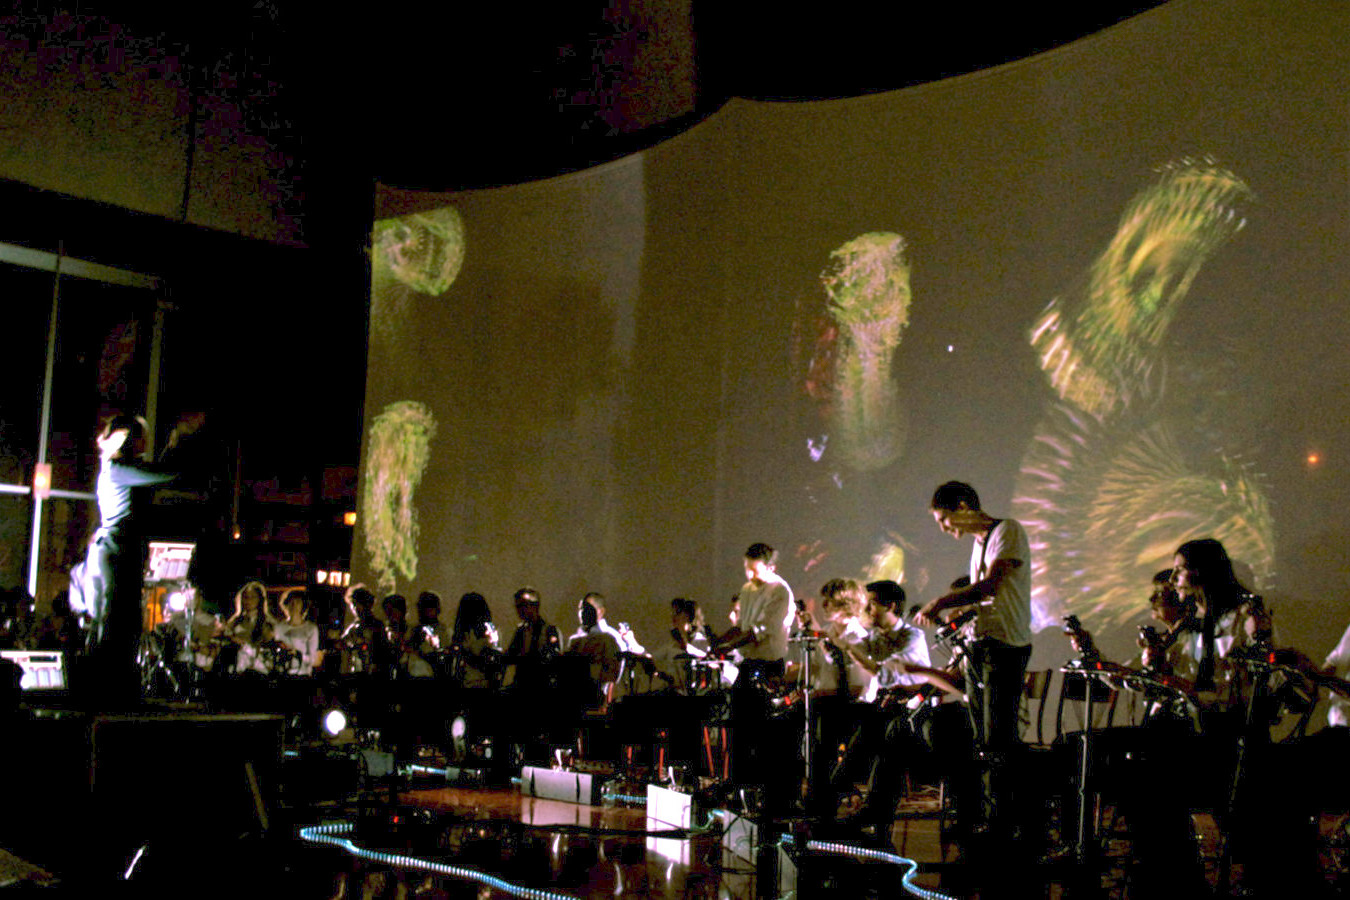
\includegraphics[width=\linewidth]{gfx/02_ephemeral/MetaOrchestre.jpg}
		\caption[Méta-Orchestre, jouant collectivement sur le logiciel Méta-Mallette]{Le Méta-Orchestre de PuceMuse, jouant collectivement sur le logiciel Méta-Mallette. Photographie \copyright Puce Muse.}
		\label{fig:ephemeral:meta-orchestre}
	\end{minipage}
	\hspace{.02\linewidth}
	\begin{minipage}[t]{0.48\textwidth}
	  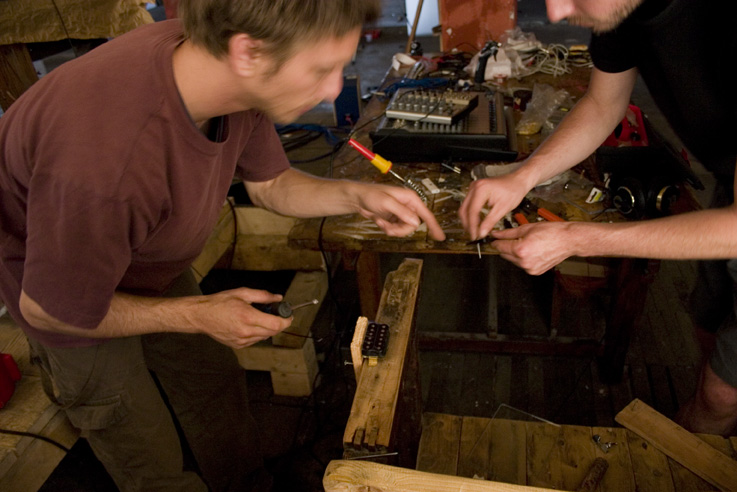
\includegraphics[width=\linewidth]{gfx/02_ephemeral/MediaMusicRoom.jpg}
		\caption[Media Music rooM, transformation collective d'un lieu en instrument de musique]{Media Music rooM, un projet de l'auteur visant à transformer collectivement un lieu en instrument de musique collectif. Photographie : Ivo Ivanov.}
		\label{fig:ephemeral:mediamusicroom}
	\end{minipage}
\end{figure}
%------------------ Figure : collective instruments ---------------------
\index[people]{goudard@Goudard, Vincent!mediamusicroom@\textit{Media Music Room}}
%---
\subsubsection{DIY-DMI}

\noindent Le \gls{DIY}, en tant qu'approche autonome et empirique, voire sauvage, de la fabrication est associée au mouvement du \gls{circuit-bending}, consistant à détourner des équipements électroniques à des fins musicales, plutôt qu'à concevoir des instruments de toute pièce. Ce mouvement s'est développé dans les années 1970, en raison de la disponibilité croissante d'appareils électroniques domestiques bon marché et l'inaccessibilité économique des synthétiseurs professionnels, donnant lieu conjointement à une nouvelle esthétique musicale, comme le note Nicolas Collins\footnote{Auteur de l'ouvrage ``Handmade Electronic Music''~\cite{collins_handmade_2006} qui accompagna la seconde vague de \gls{DIY} dans les années 2000.} : \iquote{(...) il y a eu une sorte de mouvement, en Amérique, de circuits faits maison et faits à la main pour la musique et la raison en était principalement économique, car les équipements de musique électroniques de l'époque, les synthétiseurs, étaient trop chers pour qu'on puisse les acheter. (...) Mais alors un mouvement a commencé autour d'une sorte de musique électronique alternative, qui n'était pas tant basée sur l'utilisation du son électronique dans la perspective de réaliser une vision préalable que, selon les termes de David Tudor, `composer à l'intérieur de l'électronique'.} \footnote{\iquote{(...) there was a kind of a movement in America of homemade and handmade circuitry for music and the reason was that it was primarily economic, which is that the electronic music equipment of the time, synthesizers, were too expensive for a person to buy. (...) But then a kind of a movement started about a kind of an alternative electronic music that was based not so much on using electronic sound to realize an existing vision but as David Tudor called it: `composing inside electronics'.} (cf. Annexe \ref{appendix:collins})}\\
\indent Par la suite, l'arrivée au début des années 2000 de micro-contrôleurs facilement programmables et bon marché\footnote{La figure \ref{fig:ephemeral:DIY-devices} témoigne de l'évolution fulgurante de l'accessibilité de ces technologies : l'Eobody, interface d'acquisition de capteurs commercialisée en 2003 pour environ 300€; l'arduino, programmable et offrant des fonctions similaires, commercialisé en 2005 pour quelques dizaines d'euros seulement; le Raspberry Pi commercialisé en 2013 propose pour 35€ un nano-ordinateur de la taille d'un arduino; la plateforme BeagleBone+Bela commercialisée en 2016 permet pour 100€ de disposer d'un nano-ordinateur et une interface audio à latence ultra-faible dans le même facteur de forme.} (cf. figure \ref{fig:ephemeral:DIY-devices}), ainsi que le développement de forums d'échange d'information sur Internet a renouvelé la pratique \gls{DIY}, avec des cartes électroniques telles qu'arduino\footnote{\url{https://www.arduino.cc}}, et des nano-ordinateurs tels que Teensy\footnote{\url{https://www.pjrc.com}}, Raspberry Pi\footnote{\url{https://www.raspberrypi.org}}, Bela\footnote{\url{https://www.bela.io}}, etc. Ce second mouvement a également été accompagné par l'émergence de \glspl{makerspace} et de \glspl{fab-lab}.
%------------------ Figure : DIY-LiveCoding ---------------------
\begin{figure}[!htbp]
	\captionsetup{format=plain}%
	\centering
	\begin{minipage}[t]{0.48\textwidth}
		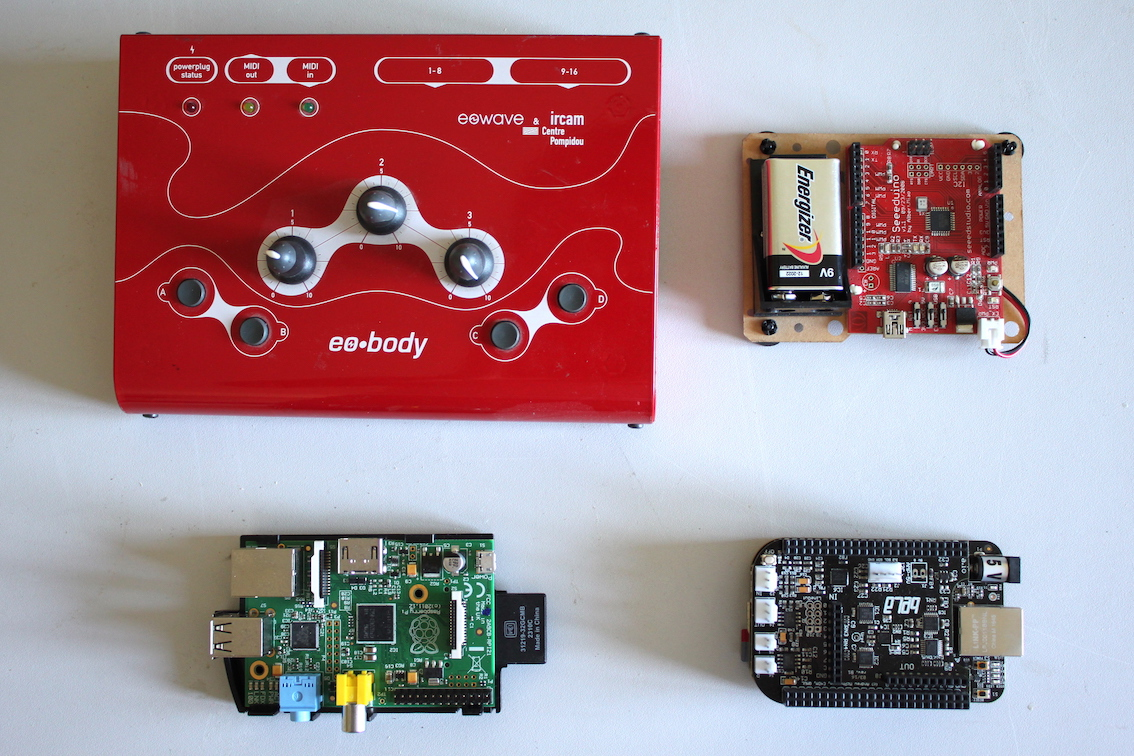
\includegraphics[width=\linewidth]{gfx/02_ephemeral/Eobody-arduino-raspi-bela_144px.jpg}
		\caption[Eobody, Arduino, Raspberry Pi, Bela]{De haut en bas et de gauche à droite: Eobody, Arduino, Raspberry Pi, Bela.}
		\label{fig:ephemeral:DIY-devices}
	\end{minipage}
	\hspace{.02\linewidth}
	\begin{minipage}[t]{0.48\textwidth}
	  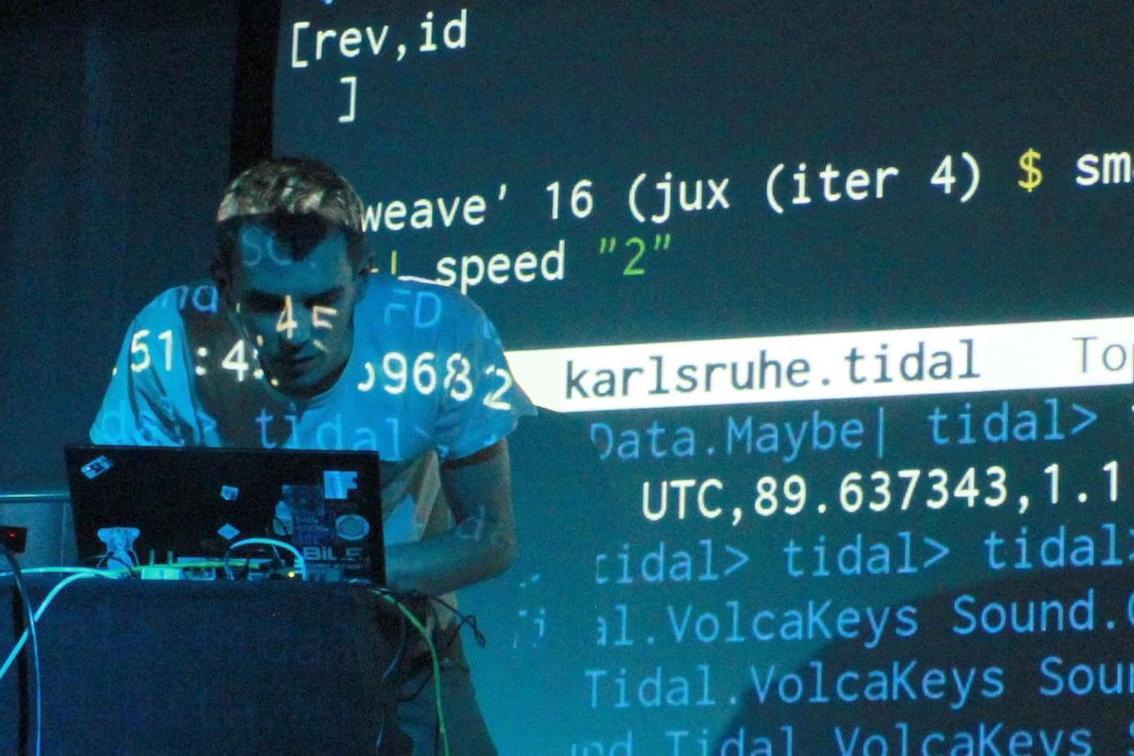
\includegraphics[width=\linewidth]{gfx/02_ephemeral/alex_mclean_144px.jpg}
		\caption[Alex McLean, live-coding avec le langage Tidal Cycles]{Alex McLean, live-coding avec le langage Tidal Cycles.}
		\label{fig:ephemeral:livecoding}
	\end{minipage}
\end{figure}
%------------------ Figure : DIY-LiveCoding ---------------------
\index[people]{mclean@McLean, Alex}

%--------------------------------------------------------------
\subsubsection{Live Coding}

\noindent Le \textit{live coding} s'est développé au début des années 2000, comme une pratique visant à créer en direct et de manière semi-improvisée des programmes de création musicale. Cette pratique a été rendue possible par l'orientation de certains logiciels dans une optique de performance live, en particulier SuperCollider \cite{mccartney_rethinking_2002} et le développement dans cette même perspective de logiciels tels que ChucK\footnote{créé à l'université de Princeton par Ge Wang and Perry Cook, voir \cite{wang_chuck_2003}.} en 2003, ou TidalCycles\footnote{créé par Alex McLean, voir \cite{mclean_tidalpattern_2010}, \url{https://tidalcycles.org}.} en 2009, permettant l'interprétation à la volée de code créant et contrôlant des modules de synthèse\footnote{Une liste relativement exhaustive de langage de \textit{live coding} est disponible ici : \url{https://github.com/toplap/awesome-livecoding}.}. Ce mouvement s'est également structuré dans une communauté d'échange sur Internet soutenue en particulier par l'association TOPLAP\footnote{\url{https://toplap.org}} et depuis 2015 l'\gls{ICLC}. Le live-coding est une pratique musicale vivante et active, dont le langage de programmation constitue l'instrument \cite{blackwell_programming_2005} et dont l'interface de jeu est souvent le clavier d'ordinateur.\\

%--------------------------------------------------------------

\subsubsection{Installations sonores et instruments à la frontière}

\noindent Enfin, dans la prolifération croissante de systèmes sonores et musicaux qui caractérise ce dernier siècle, les installations sonores interactives constituent une autre forme d'expérience participative du sonore, que celle généralement associée à l'idée d'instrument de musique. A mi-chemin entre la composition, la sculpture et l'instrument, elles ne permettent souvent qu'une pratique éphémère et/ou partielle de la musique (ou simplement du son) donnée à entendre. Elles représentent toutefois un axe révélateur des nouveaux termes dans lesquels la musique et l'instrument s'inscrivent dans la société, en rapprochant les rôles de l'instrumentiste et de l'auditeur, en imbriquant la notion d'instrument et de composition, et en déplaçant la notion de concert et de performance.\\
\indent Ce qu'on appelle généralement ``installation sonore'' conserve toutefois l'idée d'un lieu et d'un moment consacré à l'écoute (ainsi que l'idée d'un artiste auteur), mais l'autonomie propre à l'instrument électrique l'a progressivement entraîné --~depuis un siècle déjà~-- hors des cadres ``concertants'', dans des usages personnels hybrides entre instruments d'écoute et de performance (des bandes magnétiques au web-streaming\footnote{Voir notamment, dans des perspectives différentes d'utilisations musicales du réseau, les projets \textit{WJ-S} d'Anne Roquigny\index[people]{roquigny@Roquigny, Anne!wjs@\textit{WJ-S}} (\url{https://www.wj-s.org}), les mashups Youtube de Kutiman\index[people]{kutiman@Kutiman (Kutiel, Ophir, alias~—)!thruyou@\textit{ThruYOU}} (\url{https://youtu.be/WoHxoz_0ykI}), les sonifications du web par le collectif d'artistes \textit{Art of Failure}\index[people]{artoffailure@Art of Failure (groupe)} \url{http://artoffailure.free.fr} ou encore les fragments de code audio-génératifs postés sous forme de tweets du projet \textit{sc140} \url{https://twitter.com/sc140tweets}. Pour une réflexion stimulante sur la question des pratiques musicales en réseau, voir notamment \cite{joy_epoque_2009}.}, en passant évidemment par la platine vinyle) qui se prolongent dans la prolifération des \textit{apps}\footnote{Comme l'application RjDj, une des premières ayant souligné cette hybridation sur les smartphones.} audio-musicales sur les ordinateurs mobiles.
%--------------------------------------------------------------
\subsection{Musical organics}
\label{sec:ephemerality:musical-organics}

\noindent On voit que la diversité des lutheries numériques rend leur classification problématique, autant que celle des instruments acoustiques classiques qui se retrouvent augmentés. Pourtant, une telle classification peut être souhaitable, dans la mesure où elle fournit un cadre référentiel d'échange et de discussion entre luthiers, des critères d'analyse pour le musicologue, ainsi que des points de repère pour le compositeur souhaitant travailler avec de tels instruments. \\
\indent Parmi les différentes proposition d'organologie des \glspl{DMI}, celle proposée par Thor Magnusson dans \cite{magnusson_musical_2017} qu'il nomme \textit{Musical Organics}\footnote{L'expression se traduit difficilement en français, le terme \textit{organics} renvoyant à l'idée d'organologie autant qu'à l'idée d'organicité, i.e. l'organisation d'un être ``vivant''.} semble particulièrement intéressante en ce qu'elle considère l'organisation des instruments de musique en fonction de l'agencement ``organique'' de leurs éléments.\\
\indent Cette classification propose ainsi d'adopter un modèle rhizomatique, représentant de manière plus adaptée les connexions qui se créent entre différents ``organes'' constitutifs d'un instrument, qu'ils soient \textit{matériaux} (e.g. plastique, métal, verre, etc.), \textit{capteurs} (e.g. \gls{FSR}, microphones, potentiomètres, etc.), \textit{sons} (e.g. échantillons, synthèse FM, additive, etc.), \textit{\glspl{mapping}} (e.g. fonctions de transfert, apprentissage, stochastique, etc.), \textit{gestes} (e.g. frapper, pincer, frotter, etc.), ou tout autre aspect culturel, technique, musicologique ou appartenant à un quelconque domaine entretenant un lien avec la lutherie.\\
\indent Magnusson note que cette organisation, au-delà de l'aspect descriptif déjà présent dans les organologies traditionnelles, devrait se prêter à une \iquote{organologie interprétative, qui pose les questions du `pourquoi' et du `comment', et offre des explications en replaçant ces questions dans leurs contextes historiques et musicologiques.}

%%%%%%%%%%%%%%%%%%%%%%%%%%%%%%%%%%%%%%%%%%%%%%%%%%%%%%%%%%%%%%%
\section{Une critique de la longévité}
\label{sec:ephemerality:critique}

\noindent Ce foisonnement dans le paysage des \glspl{DMI} et la difficulté à établir des catégories qui se raccordent avec les classifications classiques coïncident avec une question plus générale portant sur la longévité de ces instruments. En effet, comment établir des catégories si les objets que l'on souhaite classer sont en mutation permanente ? Et comment partager, transmettre, enseigner, pratiquer la musique avec des objets aussi instables ?

\subsection{DMI will survive}

\noindent La longévité des \glspl{DMI} est une question complexe qui a été soulevée à plusieurs reprises dans la littérature des \gls{NIME} (et d'autres domaines connexes) et fait l'objet d'un débat croissant au cours de la dernière décennie \cite{baguyos_contemporary_2014, morreale_design_2017,bonardi_preservation_2008}. Les auteurs qui se sont intéressés à cette question ont identifié un certain nombre de causes de cette situation, qu'elles soient techniques, méthodologiques ou sociologiques, et ont apporté réflexions et propositions pour y remédier, telles que de nouveaux environnements pour concevoir et évaluer les instruments \cite{jorda_digital_2004, morreale_design_2017}, une meilleure documentation, de nouvelles méthodes pédagogiques et la création de communautés, ainsi qu'un travail visant à établir une notation musicale et un répertoire pour ces nouveaux instruments \cite{mamedes_composing_2014,mays_notation_2014}. Cependant, dans la majorité de ces articles, le manque de longévité des \glspl{DMI} est essentiellement considéré comme un défaut, ou du moins un problème à résoudre.\\
\indent Dès 1975, des compositeurs de musique électroacoustique au \gls{GRM} réfléchissaient aux questions de préservation soulevées par une musique \iquote{écrite sur du sable}\footnote{Michel Chion\index[people]{chion@Chion, Michel} emploie cette formule dans \cite{chion_musique_1977}, en faisant référence aux particules ferro-magnétiques des bandes audio, vouées à une dégradation prochaine.} : certains compositeurs disaient qu'ils s'en moquaient et faisaient leur musique pour le présent, tandis que d'autres voyaient dans l'ère numérique naissante la possibilité de préserver leurs œuvres dans le futur. Comme nous le savons aujourd'hui, troquer le sable contre le silicium (ou le nuage, maintenant) n'a pas totalement résolu le problème.\\
\indent Les \glspl{DMI} ayant largement intégré la partie compositionnelle des œuvres musicales, parfois même confondue avec l'instrument, le désir de préserver les œuvres musicales s'est trouvé partiellement transposé dans la question de la conservation des instruments et des outils utilisés pour leur production. Mais quelles sont les raisons de cette quête de longévité ? Et qu’est-ce qui légitime à ce point la longévité d’un instrument pour qu’elle soit d’emblée vue comme une qualité ?\\
\indent Le désir de longévité est ontologiquement lié à une réaction profondément enracinée dans notre condition de simples mortels, qui consiste à chercher un moyen d'assurer notre survie, notamment par la transmission des connaissances et la création de traditions. Le paléoanthroplogue André Leroi-Gourhan a analysé le phénomène des traditions comme un moyen d'extérioriser et de transmettre notre mémoire à travers la création de systèmes techniques et de ``chaînes opératoires'' \cite{leroi-gourhan_geste_1964}. Plus récemment, Bernard Stiegler s'est appuyé sur cette idée pour définir le concept de ``grammatisation'', comme processus par lequel le \textit{continuum} temporel des comportements humains est transformé en un spatial discret, ce qui permet de les intégrer dans des outils \cite{stiegler_for_2010}.\\
\indent Les humains ont ainsi développé des méthodes et des outils, tels que la psalmodie de textes (surtout religieux) ou l'écriture comme moyens à la fois d'enregistrer des informations pour un usage ultérieur et de transmettre des connaissances à ceux qui y survivent. L'écriture a partiellement libéré les humains du besoin de tradition orale en transférant ces connaissances sur un support physique, ce qui lui a également permis de capitaliser et de spéculer sur ses connaissances.\\
\indent Ainsi, la notion de longévité traverse le champ des arts et des sciences, aux frontières desquels se trouvent les instruments de musique. Dans l'histoire de l'art, il reste principalement les œuvres durables, ``gravées dans le marbre'', dont sont faites les sculptures. De même, la science aspire à trouver des lois durables pour décrire le monde observable et les formuler dans le langage pérenne des mathématiques. Mais si la longévité évidente d'une œuvre constitue souvent un atout pour sa propre légitimation, lorsqu'il s'agit d'un instrument numérique et plus encore lorsqu'il est conçu comme un moyen interactif de créer une expérience musicale par essence éphémère, la question ne semble pas pouvoir se régler dans les mêmes termes.\\

	
\subsection{Longevité, adoption, succès}

\noindent Deux aspects semblent être souvent confondus : la longévité d'un instrument d'une part et son ``succès'' d'autre part. De plus, la notion de succès, éminemment sujette à la perspective adoptée, semble être souvent considérée comme le taux d'adoption par une communauté d'instrumentistes, au-delà des aspects financiers d'un succès commercial.\\
\indent Ces trois aspects, longévité, succès et adoption, sont cependant relativement différents, en partie indépendants et parfois même contradictoires. Il existe des exemples notoires de ce décalage: \textit{The Hands} de Michel Waisvisz\index[people]{waisvisz@Waisvisz, Michel} \cite{torre_hands:_2016} (Figure \ref{fig:ephemeral:Waisvisz_TheHands}), le \textit{Lady's Glove} de Laetitia Sonami\index[people]{sonami@Sonami, Laetitia} \cite{sonami_my_2006} (Figure \ref{fig:ephemeral:Sonami_LadysGlove}) ou encore le \textit{Méta-Instrument} de Serge De Laubier\index[people]{delaubier@De Laubier, Serge} \cite{couprie_meta-instrument:_2018} (Figure \ref{fig:ephemeral:DeLaubier_MI4}) sont trois instruments ayant eu une longévité remarquable\footnote{Plus de 20 ans pour \textit{The Hands} --~jusqu'au décès de Michel Waisvisz, 28 ans pour le \textit{Lady's Glove} et plus de 30 ans pour le \textit{Méta-Instrument} dont l'actuelle 4\textsuperscript{e} version a été finalisée en 2019.}, soutenue par une pratique régulière de leur inventeurs, sans toutefois avoir été adoptés par une large communauté d'instrumentistes. Inversement, l'éphémérité d'un outil ne mène pas systématiquement à une absence de popularité\footnote{Considérons ici tous les gadgets éphémères qui, sous l'influence d'une mode et/ou d'une puissante campagne publicitaire, envahissent le marché, ou encore tous les appareils qui deviennent obsolètes lorsqu'un nouvel appareil les remplace, tels que le smartphone qui, outre le remplacement de nos anciens téléphones, a également balayé d'un coup les lecteurs mp3, les GPS, les consoles de jeux portables, les lampes de poche, les montres, etc.} et encore moins à un manque d'intérêt musical pour les performances réalisées avec ces instruments.\\
%------------------ Figure : Waisvisz — De Laubier ---------------------
\begin{figure}[!htbp]
	\captionsetup{format=plain}%
	\makebox[\linewidth][c]{%
		\begin{subfigure}[b]{.35\textwidth}
			\centering
			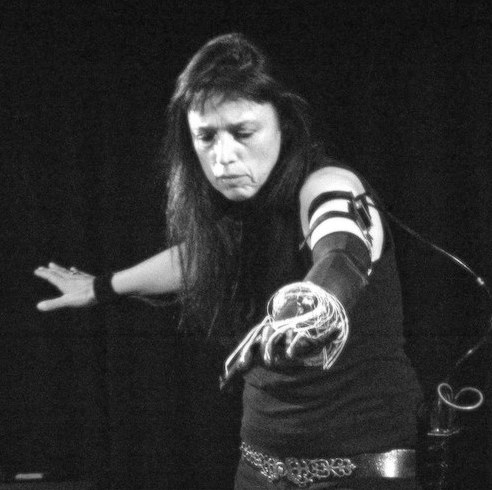
\includegraphics[width=.98\textwidth]{gfx/02_ephemeral/Sonami.jpg}
			\caption[Laetitia Sonami et le Lady's Glove]{L. Sonami: Lady's Glove\\ photographie: Charles Kremenak}
			\label{fig:ephemeral:Sonami_LadysGlove}
		\end{subfigure}%
		\begin{subfigure}[b]{.35\textwidth}
			\centering
			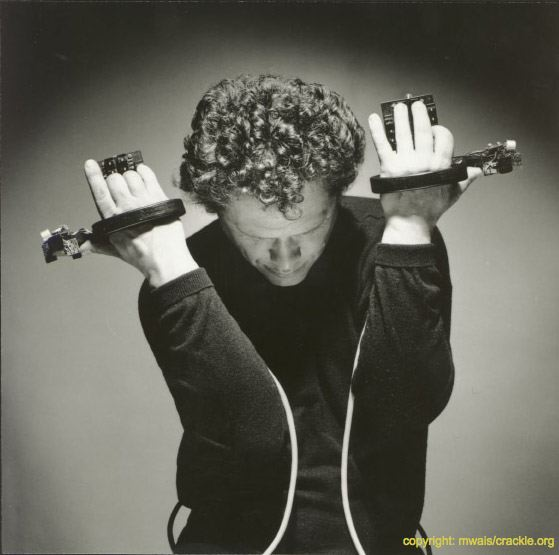
\includegraphics[width=.98\textwidth]{gfx/02_ephemeral/Waisvisz_TheHands.jpg}
			\caption[Michel Waisvisz et The Hands v2]{M. Waisvisz: The Hands\\ photographie: Carla van Thijn}
			\label{fig:ephemeral:Waisvisz_TheHands}
		\end{subfigure}%
		\begin{subfigure}[b]{.35\textwidth}
			\centering
			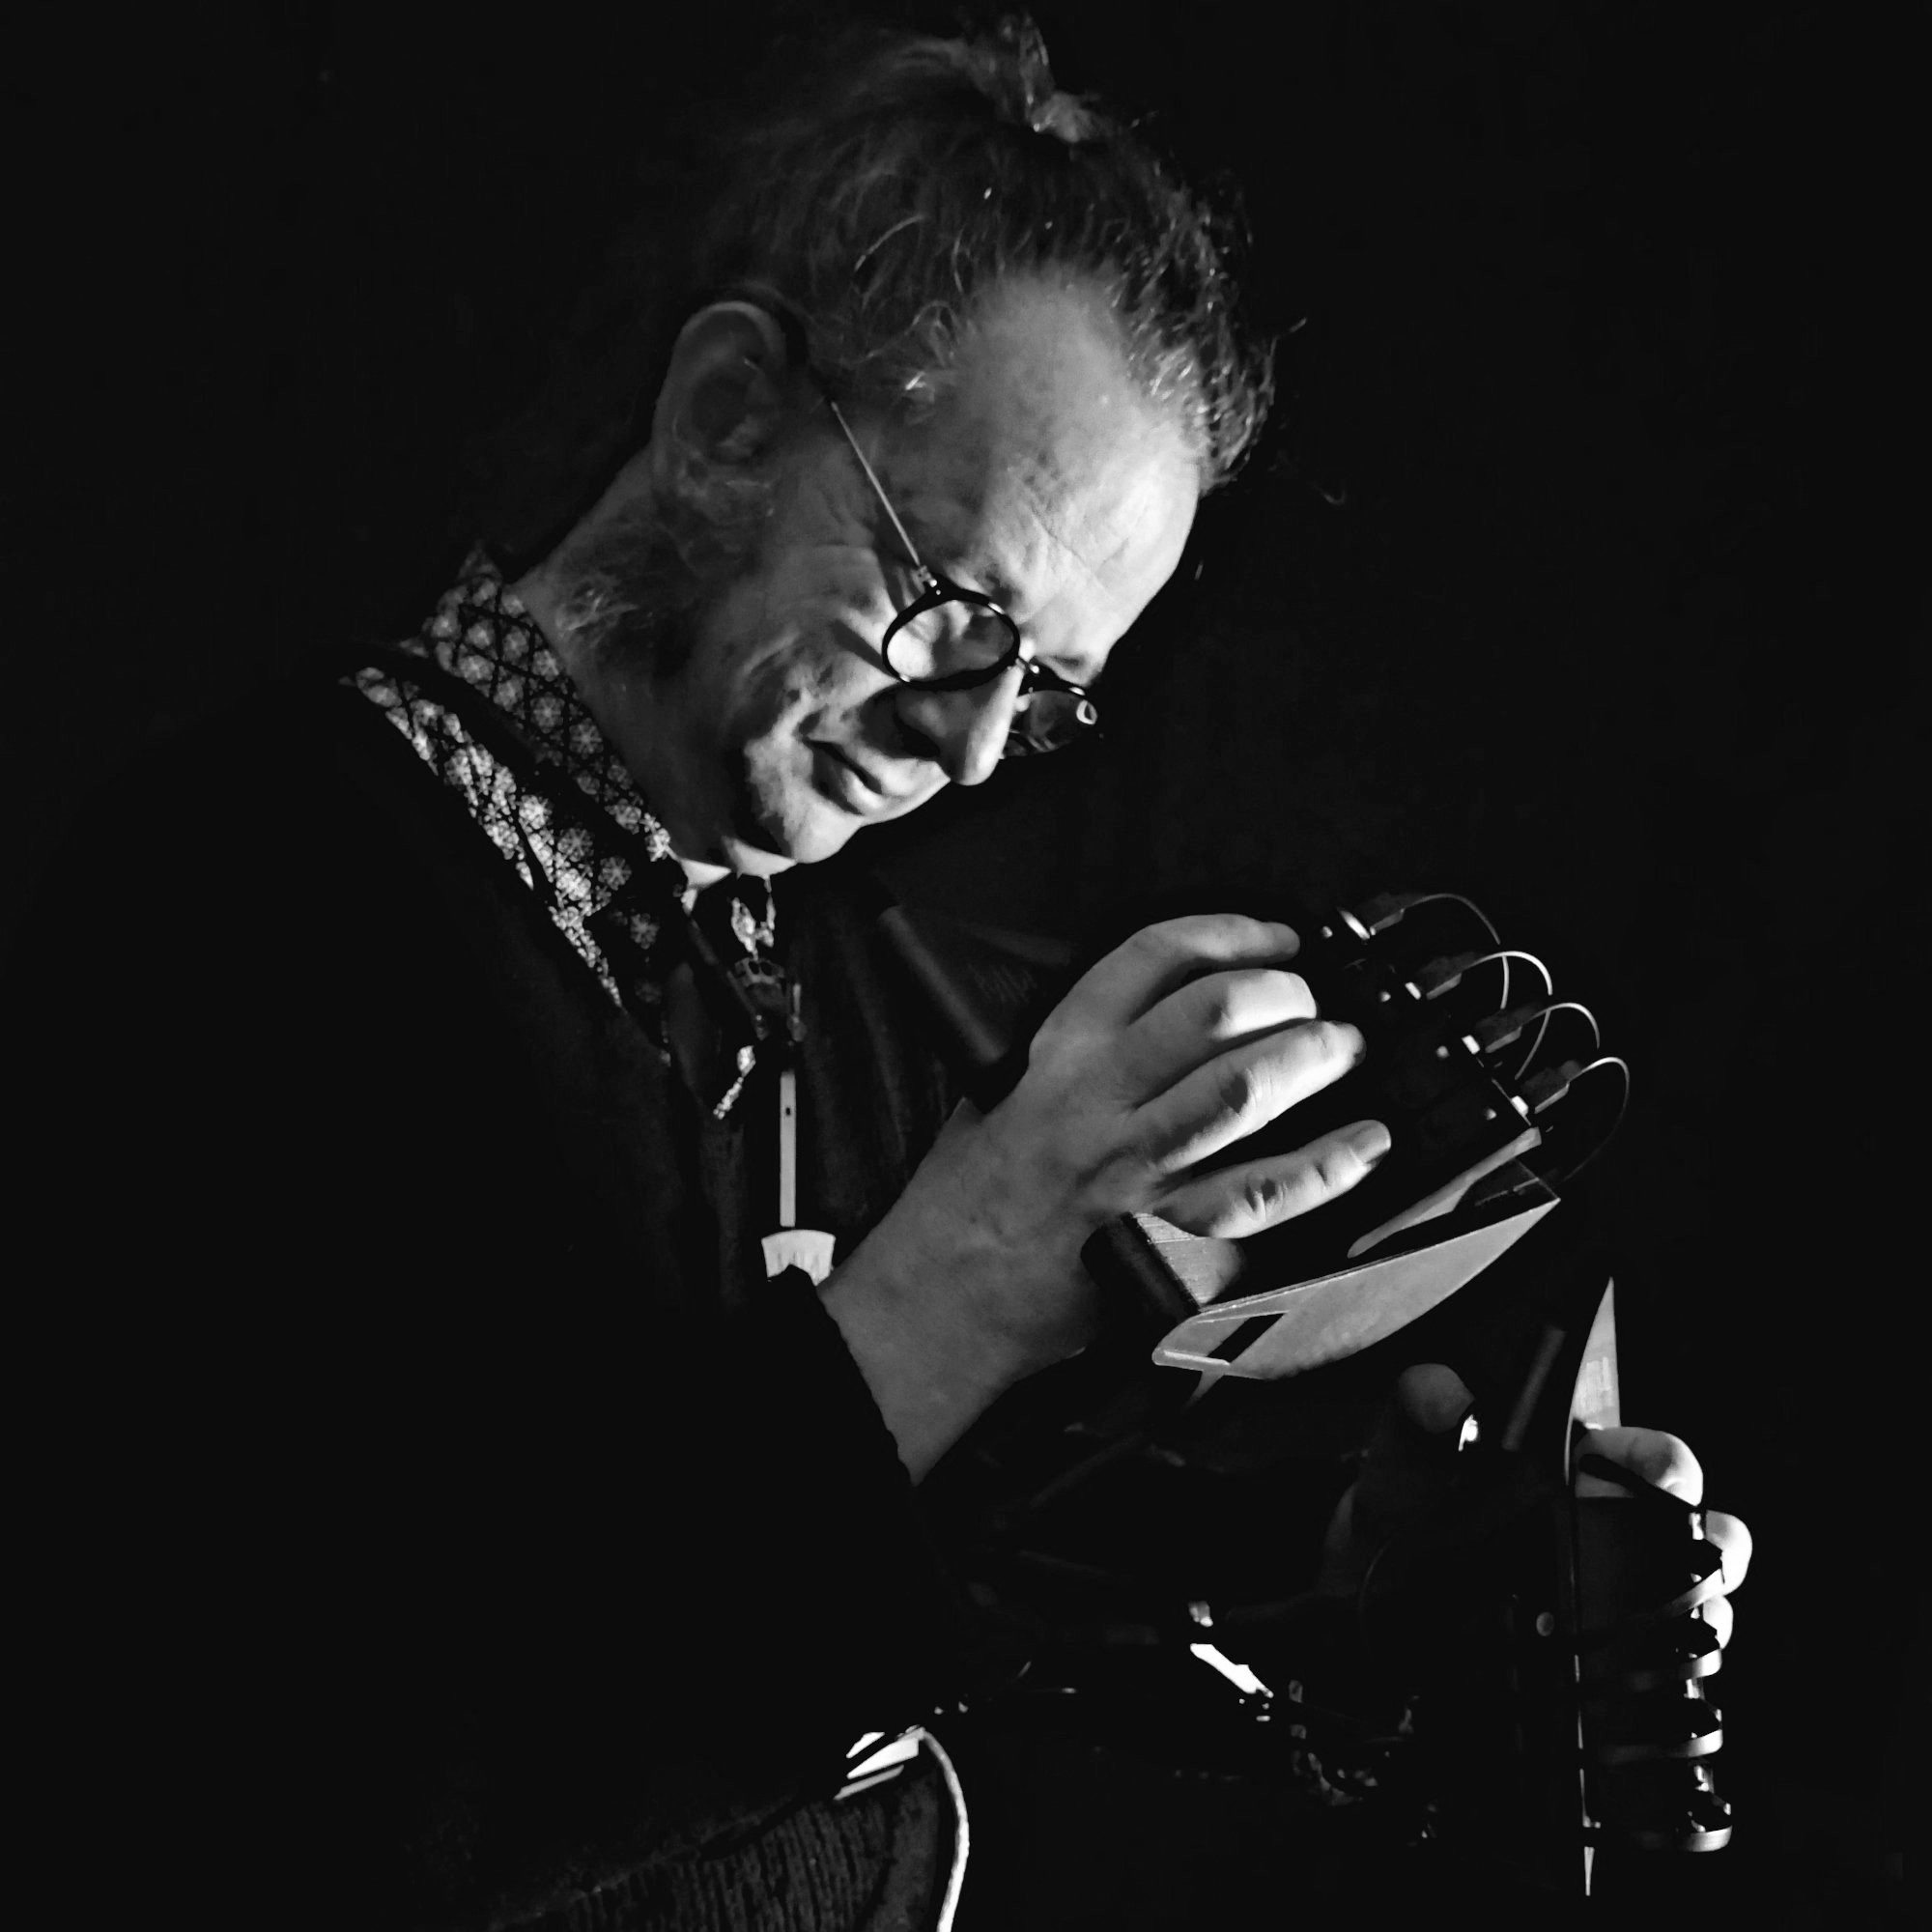
\includegraphics[width=.98\textwidth]{gfx/02_ephemeral/DeLaubier-MI4.jpg}
			\caption[Serge de Laubier et le Méta-Instrument 4]{S. de Laubier: Méta-Instrument\\ photographie: Puce Muse}
			\label{fig:ephemeral:DeLaubier_MI4}
		\end{subfigure}%
	}
	\caption[Lady's Glove, The Hands, Méta-Instrument: durabilité n'est pas synonyme d'adoption]{\textit{Lady's Glove}, \textit{The Hands}, \textit{Méta-Instrument}: durabilité n'est pas synonyme d'adoption par un large public.}
\end{figure}
%------------------ Figure : Waisvisz — De Laubier ---------------------
\indent La notion de succès dépend ainsi de la perspective adoptée, selon qu'elle soit celle des luthiers qui créent des instruments pour d'autres ou de ceux qui créent des instruments pour eux-mêmes\footnote{L'étude de Morreale et McPherson \cite{morreale_design_2017} tend à montrer une majorité des seconds dans les participants à la conférence \gls{NIME}}. Dans ce dernier cas, l'adaptation de l'instrument aux besoins ou à l'esthétique propres de l'instrumentiste peut s'avérer telle qu'il soit difficile pour les autres de l'adopter.\\
\indent Également, les évolutions techniques ainsi que les modes peuvent amener à la réapparition d'instruments tombés dans l'oubli. On appréciera ici la perspicacité de François-Alexandre Garsault, cité par Malou Haine \cite{haine_les_2018}, qui dans sa ``Division des instruments selon leurs différentes utilisations'' (1761) classait une série d'instruments, dont la harpe et la ``guitare'' (sic), dans la catégorie des \iquote{Instruments hors d'usage, mais qui peuvent revenir}.


\subsection{Longevité versus stabilité}
\label{sec:ephemeral:longevity_stability}

\noindent La question de la durabilité d'un instrument soulève implicitement la question de sa stabilité historique. Ainsi, l'histoire organologique des instruments de musique européens révèle de nombreux facteurs qui conduisent à l'apparition, à l'évolution ou à la disparition des instruments de musique. À cet égard, les nombreuses innovations technologiques de la révolution industrielle s'avèrent intéressantes car cette période bien documentée illustre les débuts des grandes révolutions qui allaient se produire au \siecle{20}~siècle, tout en soulevant la question même de la stabilité de la forme des instruments. Ainsi, lorsque le traverso fut équipé du système de clétage inventé par Théobald Boehm en 1832 et devint une flûte traversière, s'agissait-il d'un nouvel instrument ? À quel moment décidons-nous qu'un instrument qui subit des changements n'est plus le même ?

\subsection{Éphémérité dans le contexte musical}
\label{sec:ephemeral:ephemerality_in_musical_context}

\subsubsection{Impermanence du phénomène sonore}
\noindent Rappelons tout d'abord une évidence : la musique elle-même est intrinsèquement intangible, évanescente et nécessite une énergie entretenue pour exister : le phénomène sonore est en éphémérité permanente. La musique, dans sa forme sensible, n'existe que pendant le temps de sa performance. Bien que les instruments utilisés pour la produire puissent être durables, leur convocation et le son lui-même sont toujours temporaires\footnote{À tel point que les pièces qui mettent au défi cette éphémérité, telles que les \textit{Vexations} d'Erik Satie\index[people]{satie@Satie, Erik!vexations@\textit{Vexations}} ou encore \textit{Organ²/ASLSP} de John Cage\index[people]{cage@Cage, John!organ@\textit{Organ²/ASLSP}} sont des exceptions notoires.}.

\subsubsection{De la performance}

\noindent Même lorsqu'elle est notée sur une partition, la musique en tant qu'art vivant est en constante réinterprétation. Cette interprétation permet de transformer une partition notée sous forme symbolique en une expression sensible sujette à variations. On peut objecter que cette interprétation n'existe que lorsque la musique est notée de manière symbolique, laissant aux interprètes la possibilité de la jouer à leur façon dans le contexte de l'interprétation. Mais est-ce toujours le cas lorsque la musique est `intégralement notée' jusqu'au son lui-même, comme c'est le cas sur un disque audio ? Cela signifie-t-il que l'interprétation disparaît ? Les performances de spatialisation en direct de la musique électroacoustique par des musiciens professionnels ou les différentes pratiques de remixes que l'on retrouve dans le hip-hop tendent à prouver le contraire. Toute performance musicale, même la simple écoute d'un disque, convoque inévitablement un nouveau contexte d'écoute, car elle se produit nécessairement dans un moment présent unique. Entre le son enregistré et son écoute, on retrouve la même \textit{différance}\footnote{La \textit{Différance} est un concept proposé par Derrida \cite{derrida_lecriture_2014} pour désigner à la fois l'ajournement (le fait de différer) et la différenciation qui se créé entre un texte et sa signification.} qu'entre une partition et ses interprétations.

\subsubsection{Une esthétique musicale mûe par le mouvement}

\noindent Par ailleurs, la musique contemporaine occidentale poursuit une quête de la nouveauté et de territoires sonores inexplorés, comme le soulignait Jean-Claude Risset dans son discours invité à Athènes en 2014 : \iquote{(...) la musique contemporaine met en évidence ce qui a été rejeté dans le monde grec : elle capte davantage l'évanescent, l'éphémère, l'ambivalent, l'Erebus, elle favorise la métamorphose sans fin des qualités et des formes; comme Nietzsche l'a déclaré, la musique occidentale tend vers la libération de la dimension dyonisiaque et l'acceptation du côté inacceptable des mythes}\footnote{\iquote{[Hugues] Dufourt suggest that contemporary music highlights what was rejected in the Greek world : it rather captures the evanescent, the ephemeral, the ambivalent, the Erebus, it favors the endless metamorphosis of qualities and forms; as Nietzsche proclaimed, western music tends toward the liberation of the dyonisiac dimension and the acceptance of the inacceptable part of myths.} \cite{risset_sound_2014}}.\\
%\indent Cette d'attraction pour l'éphémère et la métamorphose s'est traduite dans la recherche permanente de nouveaux modes de jeu et de nouveaux timbres de la part de l'instrumentiste et du compositeur, mais surgit également dans le travail du luthier à mesure que son outil de travail gagne une souplesse qui le rapproche de la souplesse gestuelle de l'instrumentiste ou de celle de la pensée du compositeur.


\subsubsection{Partitions dynamiques, ouvertes, ad-hoc}
\label{sec:ephemeral:longevity_stability:dynamic_scores}

\noindent Les partitions musicales sont en partie intégrées dans les \glspl{DMI}, pour lesquels Norbert Schnell et Marc Battier ont proposé le terme ``d'instruments composés'' dans \cite{schnell_introducing_2002}\footnote{L'idée d'instruments composés est toutefois plus ancienne, voir Harry Partch\index[people]{partch@Partch, Harry} ou Gordon Mumma\index[people]{mumma@Mumma, Gordon} (1967) : \iquote{My own electronic music equipment is designed as part of the process of composing my music. I am really like the composer who builds his own instruments, though most of my ``instruments'' are inseparable from the compositions themselves.}\cite{mumma_creative_1967}}. La partition elle-même a fait l'objet d'une reconfiguration plus ouverte depuis le milieu du \siecle{20}~siècle et les compositeurs ont progressivement intégré les possibilités algorithmiques dans leurs processus de création : des systèmes dynamiques et interactifs mettent en mouvement la stabilité des figures de notes. Plusieurs compositeurs\footnote{Parmi ceux qui ont écrit et analysé des partitions dynamiques, voir les œuvres de Mike Solomon\index[people]{solomon@Solomon, Mike!patchy@\textit{Patchy the autobot}}, Georg Hajdu\index[people]{hajdu@Hajdu, Georg} \cite{hajdu_disposable_2016}, Sandeep Bhagwati\index[people]{bhagwati@Bhagwati, Sandeep} \cite{bhagwati_vexations_2017} ou Jason Freeman\index[people]{freeman@Freeman, Jason} \cite{freeman_extreme_2008}.} questionnent ainsi la stabilité de la partition en utilisant l'ordinateur pour créer des instances \textit{ad hoc}, soit à l'aide d'algorithmes génératifs, soit en introduisant des parties improvisées dans des formes hybrides pour lesquelles Richard Dudas\index[people]{dudas@Dudas, Richard} propose le terme de ``comprovisation'' \cite{dudas_comprovisation:_2010}. Se pourrait-il que la technologie numérique offre ce support idéal permettant à la fois la préservation des œuvres musicales en même temps que leur mutation ?

\subsubsection{Obsolescence de la technologie}

\noindent Les matériaux utilisés pour les instruments acoustiques semblent vieillir relativement bien. Le matériel électronique vieillit mal en comparaison et le cuivre de ses circuits est plus fragile que celui des trompettes, saxophones et autres cuivres. Par ailleurs, la miniaturisation extrême des microprocesseurs les rend généralement impossibles à réparer ; ils sont souvent remplacés par de nouvelles versions possiblement incompatibles. Le code informatique, dans sa forme compilée, est tout aussi cryptique que le microprocesseur : un bloc illisible qui incarne le paradoxe de la notation informatisée par rapport au papier traditionnel - ``nous écrivons des choses que nous ne pouvons plus relire''\footnote{Kevin Slavin dans la conférence ``Comment les algorithmes façonnent notre monde'', \url{https://www.ted.com/talks/kevin_slavin_how_algorithms_shape_our_world}}. Et quand le système d'exploitation sera mis à jour, il y a des chances qu'il ne pourra plus les lire non plus.\\
\indent Dans un article où il compare les différences ontologiques entre \textit{hardware} et \textit{software}, Nicolas Collins \cite{collins_semiconducting_2013} résume leur relation au temps avec la formule : \iquote{hardware is yesterday, software is now}, ce qui pourrait se traduire par le fait que le logiciel est en permanence mis à jour tandis que le hardware est toujours dépassé. Ni l'un ni l'autre ne semble être en mesure d'offrir une continuité fiable entre le passé et l'avenir.

	
\subsubsection{Économie de la nouveauté}

\noindent A l'obsolescence de la technologie, s'ajoutent les effets de la société de consommation. Depuis plus d'un siècle, l'industrie fait de plus en plus la promotion d'un paradigme jetable en encourageant les consommateurs à \iquote{acheter pour le style, pas seulement pour les améliorations technologiques} \cite{slade_made_2006} et en organisant une obsolescence programmée.\\
\indent Ce modèle économique a également affecté celui des arts du spectacle, qui promeut la création bien plus que la reprise d'un spectacle à tel point que, comme le rappelle Georg Hajdu dans \cite{hajdu_disposable_2016} : \iquote{Les pièces connaissent rarement plus qu'une seule représentation}. De même, les résidences d'artistes sont plus souvent destinées à de nouvelles créations davantage qu'à la poursuite d'œuvres antérieures.\\
\indent Cette économie de l'obsolescence (planifiée ou non) ne favorise pas l'attachement à un instrument et, en ce qui concerne les contrôleurs \gls{MIDI} commerciaux, le plastique bon marché dont ils sont le plus souvent faits dégrade la valeur qui peut être attribuée à un instrument acoustique traditionnel. L'attachement et l'engagement avec les instruments virtuels sont également remis en question par leur nature immatérielle. La plupart des logiciels commerciaux s'orientent maintenant vers une économie basée sur l'abonnement plutôt que sur l'achat, puisque l'achat ne garantit plus ni la durabilité ni la propriété de l'objet.

	
\subsubsection{L'instrument comme compromis instable}

\noindent L'instrument de musique est aussi, comme le souligne Bernard Sève dans \cite{seve_instrument_2013} : \iquote{un compromis instable entre des qualités non-convergentes}. Pour les instruments acoustiques, ce compromis entre ergonomie gestuelle et performance acoustique, imposé par la physicalité des matériaux, est généralement fixé dans un assemblage ajusté et collé. Ce montage agit comme un facteur de stabilisation par rapport à un environnement numérique dans lequel l'absence de contraintes physiques laisse l'instrument à cœur ouvert, prêt à être modifié à tout instant.\\
\indent Bill Buxton soulignait la différence entre les spécifications standard, militaires et artistiques pour souligner l'exigence plus élevée de cette dernière \cite{buxton_artists_1997}. Le design des objets d'art exige une grande finesse, en effet. Accorder les qualités sonores et ergodynamiques\footnote{Thor Magnusson a proposé ce terme dans \cite{magnusson_ergodynamics_2019} pour nommer le \iquote{pouvoir et la profondeur expressive d'un instrument}.} d'un instrument de musique s'apparente à la quête d'un \textit{inframince}\footnote{\label{fn:inframince}Marcel Duchamp \cite{duchamp_notes_2008} a inventé le terme \textit{inframince} dans une série d'exemples décrivant une différence si infime qu'elle ne peut être qu'imaginée, par exemple \iquote{La différence entre deux objets faits en série (sortis du même moule) est un inframince quand le maximum de précision est obtenu.}} pour lequel il n'existe pas de spécifications convenues. Cependant, une autre particularité des technologies utilisées pour les performances live est qu'elles sont \iquote{dévolues à une expérience, pas à une bande-son, inutiles pour la relecture, la sauvegarde, l'échange ou la duplication}, comme le note Nicolas Collins dans \cite{collins_semiconducting_2013}.\\
\indent Ainsi, la pérennité de l'instrument en dehors de la durée même de la performance n'est pas un critère essentiel et il n'est pas rare que les musiciens numériques\footnote{Andrew Hugill définit un \textit{musicien numérique} dans \cite{hugill_digital_2008} comme \iquote{quelqu'un qui a saisi les possibilités ouvertes par les nouvelles technologies, en particulier le potentiel de l'ordinateur pour explorer, stocker, manipuler et traiter le son, ainsi que le développement de nombreux autres outils et dispositifs numériques qui permettent l'invention et la découverte musicale} soulignant le fait qu'ils sont \iquote{non pas définis par leur seule utilisation de la technologie}, mais ont aussi \iquote{une certaine curiosité, un questionnement et un engagement critique sur ce terrain}.} modifient leur instrument quelques minutes avant le début d'un concert, juste pour les besoins du moment présent.

	
\subsubsection{Esthétique du dysfonctionnement}

\noindent En effet, le risque de dysfonctionnement n'est pas rédhibitoire à de nombreuses performances musicales. Les bugs et artefacts causés par les dysfonctionnements s'avèrent être des sources fertiles de matériaux musicaux et la subversion du fonctionnement cryptique des processeurs en révèle un aspect invisible, faisant ressurgir la nature même du matériau électronique, au-delà de l'objectif pour lequel ils ont été conçus\footnote{Parmi les exemples significatifs, les travaux de Yasuano Tone dans \textit{Solo for Wounded CD}\index[people]{tone@Tone, Yasuano!woundedcd@\textit{Solo for Wounded CD}}, ceux de Nicolas Collins\index[people]{collins@Collins, Nicolas!royaltouch@\textit{The Royal Touch}} sur circuits électroniques morts (\textit{The Royal Touch}) ou encore la sonification de données brutes par Carsten Nicolai dans \textit{Unitxt}\index[people]{noto@Noto (Nicolai, Carsten, alias~—)!unitxt@\textit{Unitxt}} illustrent clairement cette approche.}. David Zicarelli\footnote{Zicarelli est le fondateur de \textit{Cycling'74}, entreprise développant et commercialisant le logiciel Max.} le résumait en ces termes : \iquote{Je remarque simplement que dans la plupart des concerts pointus, l'échec a tendance à être beaucoup plus intéressant pour le public que le succès.}\footnote{\iquote{I would only observe that in most high- profile gigs, failure tends to be far more interesting to the audience than success.} cité par Cascone dans \cite{cascone_aesthetics_2000}.} On peut lire dans cette remarque une tendance essentielle de l'époque post-moderne, caractérisée par un art qui attribue davantage de valeur à \textit{l'intérêt} du geste pris dans un contexte \textit{expérimental}, qu'à sa \textit{qualité}, pris dans un contexte \textit{normatif} classique.

\subsubsection{Plus besoin de tradition?}

\noindent L’apparition de la notation musicale ne rend plus nécessaire la performance à seules fins de transmission, l’enregistrement audio ne rend plus nécessaire la performance à seules fins d’écoute, l’existence de banques de sons ne rend plus nécessaire l’apprentissage d’un instrument particulier pour produire le son de cet instrument\footnote{Voir par exemple, le rendu du Sacre du Printemps\index[people]{stravinsky@Stravinsky, Igor!sacreduprintemps@\textit{Le Sacre du Printemps}} d'Igor Stravinsky par Jay Bacal\index[people]{bacal@Bacal, Jay!sacreduprintemps@\textit{Le Sacre du Printemps}} avec la Vienna Sound Library (VSL): \url{https://youtu.be/PB3njyDW8SY.}} et maintenant l’intelligence artificielle rend superflu l'acte même de composition en laissant la possibilité de générer automatiquement des morceaux inédits\footnote{Voir par exemple les productions du projet FlowMachines par François Pachet et al. in \cite{hadjeres_deepbach:_2016}: “Daddy's car” (\url{https://youtu.be/LSHZ_b05W7o})\index[people]{flowmachines@FlowMachines (groupe)!daddyscar@\textit{Daddy's car}} ou “DeepBach” (\url{https://youtu.be/QiBM7-5hA6o}). L'originalité de ces compositions par \textit{IA}, techniquement basées sur l'imitation d'un corpus existant, reste cependant une question ouverte.}.\\
\indent En 1964, André Leroi-Gourhan, qui voyait dans la machine informatique la possibilité sans précédent d'externaliser la mémoire, se demandait alors ce qui adviendrait si les machines devenaient capables \iquote{[d’écrire] des pièces de théâtre parfaites, [de peindre] des tableaux inimitables} \cite{leroi-gourhan_geste_1964}. En 1992, John Cage semblait lui répondre de façon radicale : \iquote{Nous n'avons pas besoin d'avoir des traditions si nous nous libérons de la mémoire.} \cite{sebestik_ecoute_1992}\\
\indent Cependant, s'il est possible d'évoluer, comme le décrit la philosophe Christine Buci-Glucksmann dans \cite{buci-glucksmann_esthetique_2003}, d'une culture de l'objet à une culture des flux, elle remarque que dans un pays comme le Japon qui valorise positivement l'impermanence, l'éphémère a une place centrale tout en étant profondément ancré dans la tradition.\\
\indent La résolution de cet antagonisme apparent entre la position de Cage et celle de Buci-Glucksmann semble se situer dans le déplacement des objets (ou des flux, en l'occurence) soutenus par la tradition, dans la reformulation des motivations de la pérennité et de l'éphémérité. Davantage que ses calcifications stables, c'est l'étude des dynamiques à l'œuvre dans la création musicale qui pourra nous renseigner sur la manière dont s'agencent les instruments: nous risquons sinon de n'avoir que ``découpé une tranche d'histoire''\footnote{Jean During livre cet avertissement en introduction de \cite{during_quelque_1994} : \iquote{De nos jours où s'accumulent les traces tangibles des musiques passées, il faut donc renoncer à nos illusions : on n'appréhende que du changement, du mouvant, de l'instable. On croyait avoir saisi le fond stable, la structure, l'essentiel, les archétypes, mais on avait simplement découpé une tranche d'histoire.}}.

\section{Articulation du pérenne et de l'éphémère}

\subsection{Les DMI comme agencements instables et sauvages}

\noindent Le terme même de \gls{DMI}, qui a progressivement envahi la littérature des \gls{NIME}, pourrait nous laisser penser qu'il s'agit d'une catégorie bien définie alors qu'il s'agit en fait d'un méli-mélo d'objets qui n'ont de commun que leur utilisation de la computation numérique. Le biais qui en résulte dans l'évaluation de l'incapacité des \glspl{DMI} à atteindre une maturité provient du fait qu'un instrument de musique est encore souvent considéré comme un tout cohérent, devant faire preuve de longévité, à l’image des instruments acoustiques pris comme modèles.\\
\indent Pourtant, la modularité induite par l'électronique et la technologie numérique a ``atomisé'' l'intégrité de l'instrument. Cette atomisation peut être entendue à la fois dans le sens de ``détruit'' mais aussi dans le sens de ``fragmenté en éléments atomiques''. Sur scène, on constate en outre que les \glspl{DMI} s'apparentent souvent à des assemblages prototypiques fragiles\footnote{Pour une réflexion poursuivant à dessein la fragilité —et la destructibilité— des \glspl{DMI}, voir aussi \cite{berthaut_wubbles:_2014, haddad_fragile_2017}.} (cf. Figure \ref{fig:ephemeral:Gordeff}), pleins de câbles (physiques ou virtuels) prêts à être intervertis quelques minutes avant le concert, ou même pendant celui-ci. Pourquoi dans ce cas les envisager comme des monolithes durables plutôt que comme les agencements\footnote{Adoptant ici le concept de Deleuze et Guattari proposé dans \cite{deleuze_mille_1980}; voir aussi ``musical instruments as assemblage'' de Paul Theberge dans \cite{bovermann_musical_2017}.} éphémères qu’ils sont le plus souvent?\\
%\todo{évoquer la notion de behavioural objects de \cite{bown_understanding_2009}}
\indent De ce point de vue, le format académique d'une conférence telle que \gls{NIME} rend difficile la présentation des \gls{DMI} dans leur forme chaotique et leur sélection est biaisée par le fait que leurs auteurs appartiennent souvent au monde académique. Cela favorise la démonstration de critères techniques dûment réfléchis plutôt que la présentation d'un fatras de circuits et d'algorithmes connectés empiriquement et dont on ne comprend rien au fonctionnement, sinon que le musicien qui en joue fait des merveilles.\\
\indent En se confrontant à un agencement instrumental éphémère, l'instrumentiste, tout virtuose qu'il soit, se retrouve nécessairement en tension avec un instrument ``sauvage'' qu'il faut apprivoiser. Cela demande une attention gestuelle et auditive intense et la recherche de résonance avec l'instrument. (Sinon, autant composer tranquillement chez soi et fournir à l’auditeur un support sur lequel il n’aura qu’à appuyer sur la touche \textit{play}). Peut-être davantage que la longévité, on pourra y voir un critère de lutherie intéressant : la possibilité que l'instrument dérape et devienne hors de contrôle.

%-------------------------- Figure : Gordeff ----------------------------------
\begin{figure}[!htbp]
	\captionsetup{format=plain}%
	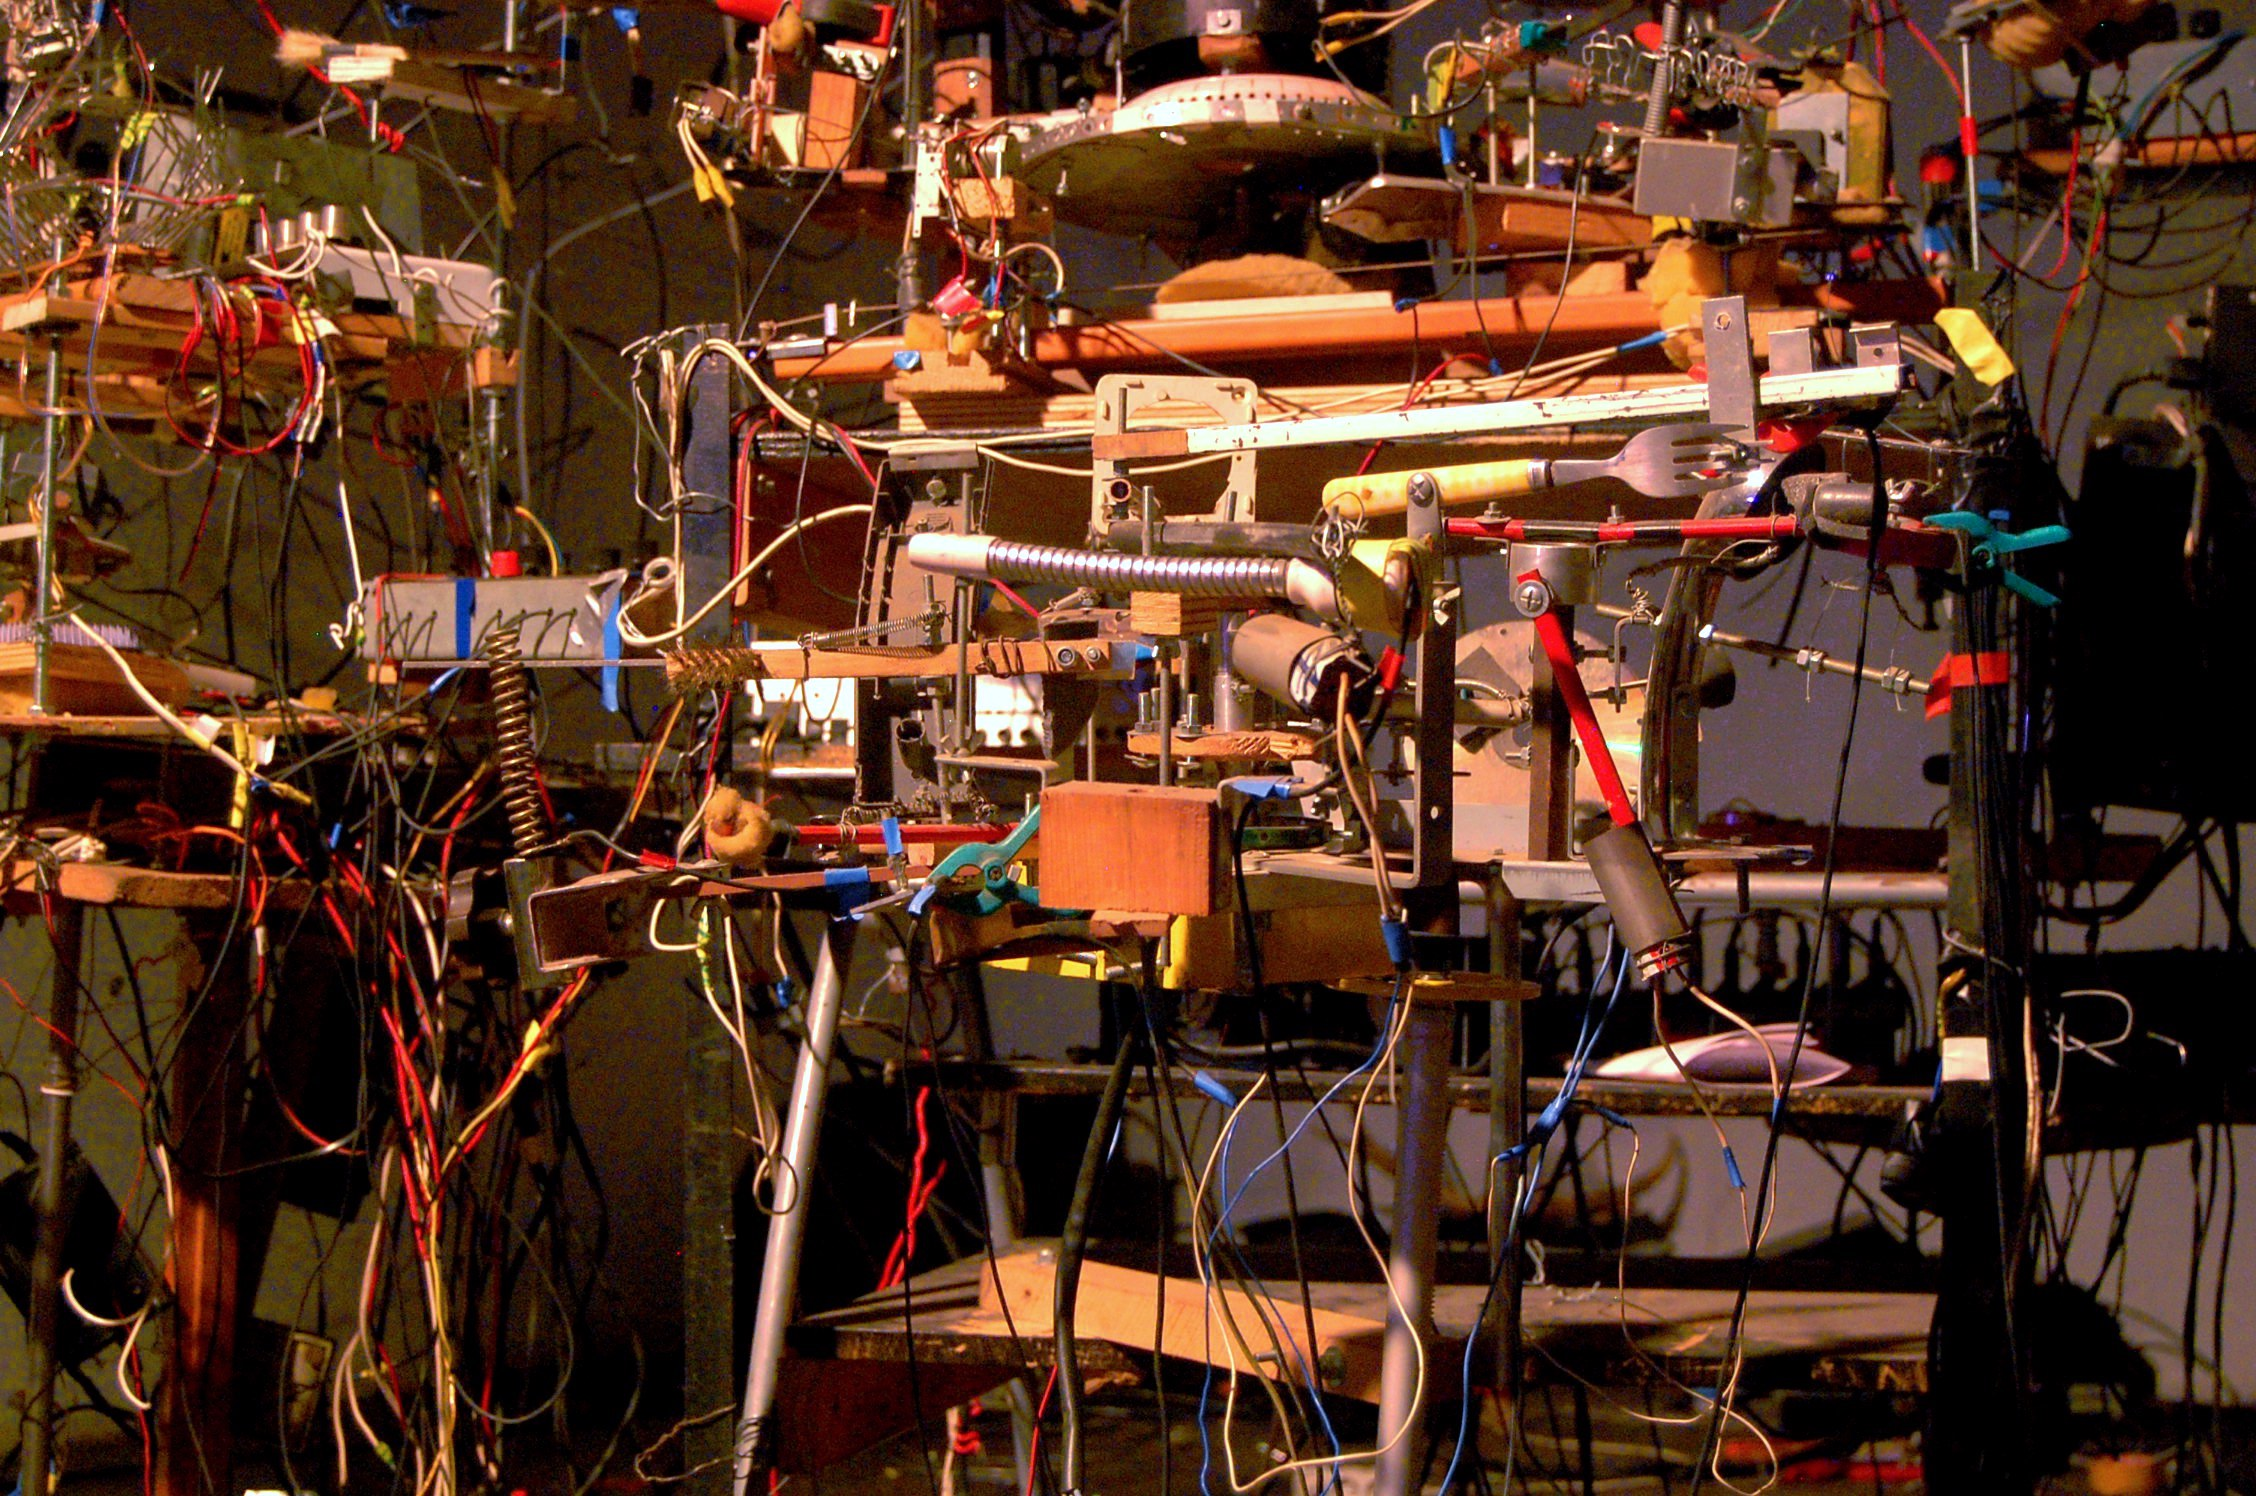
\includegraphics[width=\textwidth]{gfx/02_ephemeral/PierreGordeff.jpg}
	\caption[Détail d'un instrument de Pierre Gordeff]{Détail d'un instrument de Pierre Gordeff. Photographie : Pierre Gordeff}
	\label{fig:ephemeral:Gordeff}
\end{figure}
\index[people]{gordeff@Gordeff, Pierre}

\subsection{Cuisiner des instruments à la volée}

\noindent Une autre raison qui contribue à la stabilité des instruments acoustiques est liée à leur physicalité et à leur fabrication, qui demande un travail considérable en regard de l'arrangement virtuel de blocs logiciels - la construction d'un violoncelle requiert plus de deux mois de travail pour un luthier qui connaît son métier ! A l'inverse, John Bowers et ses collaborateurs ont promu l'utilisation d'objets prêts à l'emploi comme ``infra-instruments'' semi-fabriqués \cite{bowers_not_2005} et comme instruments ``pin-and-play'' \textit{ad hoc} \cite{bowers_creating_2006}, en repensant le cycle de vie d'un instrument avec ce type de montage éphémère et rapidement assemblé.\\
\indent Plus généralement, lorsqu'on crée un \gls{DMI} avec un environnement de programmation audio, le logiciel fournit non seulement des fonctions de base mais aussi des bibliothèques, des exemples prêts à l'emploi, complétés par d'innombrables ressources en ligne, prêtes à être téléchargées, copiées et collées.\\
\indent Cela signifie que la conception d'un \gls{DMI} peut se faire très rapidement, de manière soustractive : plutôt que de partir d'une page blanche, il est possible de chercher une version proche de ce que l'on veut réaliser et de la modifier en partant de là. Nicolas Collins a comparé cette simplicité à la cuisine, en mettant l'accent sur sa démocratisation : \iquote{Ce que ça veut dire, c'est que si tu joues en live, si tu as vraiment besoin d'instruments spécialisés, cela s'apparente presque plus à de la cuisine qu'à de la fabrication d'instruments de musique. Tout le monde cuisine, tu n'as pas besoin d'aller dans une école pour chefs !} [Collins, communication personnelle, cf. annexe \ref{appendix:collins}]\\
\indent Les évolutions récentes des langages de programmation audio tendent à aborder la question de la durabilité en créant des langages spécifiques à un domaine qui peuvent être exportés vers différentes plateformes cibles. Des cartes électroniques comme \textit{Bela} ou \textit{The Owl}\footnote{Bela: \url{https://bela.io}; The Owl: \url{https://www.rebeltech.org}} et des langages comme \gls{FAUST} développé par le \gls{GRAME} \cite{orlarey_faust_2008} ou SOUL annoncé par Roli\footnote{Announced at the Audio Developer Conference 2018. \url{https://youtu.be/-GhleKNaPdk}} reflètent tous cette tendance. Il est intéressant de noter que \gls{FAUST}, qui a été conçu dans une optique de préservation, facilite en même temps la conception d'instances éphémères en offrant à la fois un compilateur en ligne et une compilation à la volée\footnote{La compilation \textit{Just In Time} (JIT) s'appuyant notamment sur l'infrastructure \gls{LLVM}.}.
	
\subsection{Une relation tri-partite: répertoire, musicien, contexte}

\noindent Si nous cessons de considérer l'éphémérité des instruments seulement comme un problème, nous pouvons envisager la manière dont longévité et éphémérité peuvent s'articuler dans l'agentivité des pratiques liées aux \glspl{DMI}. Celles-ci peuvent être envisagées comme un assemblage tripartite entre un ensemble de matériaux, un musicien et un contexte, chacun des membres présentant un degré différent de stabilité.

\subsubsection{Le grand répertoire}

\noindent Les composants d'un \gls{DMI} peuvent être considérés comme appartenant à un large répertoire patrimonial matériel et immatériel. Ce répertoire comprend notamment tous les matériaux physiques qui peuvent être utilisés dans la construction d'instruments acoustiques : matières premières, pièces usinées ou mécaniques. \\
\indent Le répertoire immatériel est l'ensemble des connaissances théoriques et du patrimoine culturel sur lesquels on peut s'appuyer lors de la fabrication d'un instrument\footnote{Bien évidemment, la connaissance pratique est aussi essentielle à la fabrication d'un instrument, même si elle n'appartient pas vraiment au patrimoine commun auquel je fais référence ici.} : théorie musicale, connaissances scientifiques et techniques, techniques de jeu établies, répertoire musical, etc. Cette connaissance oriente le façonnement des matériaux et guide leurs positionnements relatifs :  placement des frettes, accord des cordes, disposition des touches, etc.\\
\indent Dans le cas des \gls{DMI}, cependant, le répertoire des matériaux physiques est considérablement élargi par des connaissances réifiées disponibles sous forme de matériaux numériques, soit sous forme de code informatique, soit sous forme d'ensembles de données (e.g. échantillons audio, réponses impulsionnelles, séquences de notes, etc.) qui permettent de façonner l'identité et les qualités musicales d'un instrument au-delà de ce qui est possible avec les matériaux physiques. Cet ensemble, aussi hétérogène qu'il puisse paraître, constitue un répertoire partageable dans lequel les luthiers numériques peuvent puiser les ingrédients nécessaires à la conception de leur instrument.

\subsubsection{Le musicien \textit{in-progress} / \textit{in-process}}

\noindent Le deuxième élément de l'agencement est le musicien\footnote{Ici, le terme générique de ``musicien'' représente principalement l'instrumentiste, mais comme rappelé précédemment, les frontières entre les rôles d'instrumentiste, de compositeur et de luthier sont poreuses.}. Les musiciens sont vivants et sujets au changement : leurs connaissances, leur expérience et leurs désirs, leurs compétences et leur conscience musicale, leurs projets et leurs capacités physiques évoluent tout au long de leur existence. Cette évolution se reflète dans le dispositif instrumental, par l'ajout ou le retrait de composants, ou par le développement de nouveaux instruments liés à un nouveau projet musical. Ainsi, de même que l'on peut apprendre à conduire un vélo à l'aide de roues latérales et les enlever plus tard, les \glspl{DMI} se prêtent à une assistance évolutive pour un apprentissage progressif. Cette relation co-dynamique avec l'instrument peut aider à améliorer l'intimité\footnote{Sur la question du rapport d'intimité entre le musicien et un nouvel instrument, voir notamment les articles de Sydney Fels, e.g. \cite{fels_designing_2004}.} entre le musicien et l'objet technique qui devient instrument.

\subsubsection{Le \textit{hic et nunc} de la performance}

\noindent Enfin, le \gls{DMI} peut être adapté au contexte de la performance, qui est généralement plus éphémère que les deux aspects mentionnés ci-dessus.
En composant son propre répertoire musical à partir du grand répertoire susmentionné et de sa propre expérience, le musicien sélectionne un sous-ensemble d'éléments dans la perspective d'une performance particulière, pour une proposition artistique singulière et pour s'adapter aux conditions spatiales et temporelles de la performance, ainsi qu'au public. À titre d'exemple, le code qui se duplique sans peine offre des possibilités de redimensionner un instrument soliste en instrument collectif, en distribuant le contrôle sur plusieurs interfaces. De nouveaux projets peuvent impliquer de repartir de zéro, mais les projets existants n'impliquent souvent que des ajustements contextuels plutôt qu'une reprogrammation complète de son propre système. Chris Kiefer et Thor Magnusson ont proposé le terme de ``pre-gramming'' \cite{kiefer_live_2019} pour décrire ce type particulier de préparation\footnote{Dans le contexte du live-coding qui est le leur, Kiefer et Magnusson détournent en fait le terme ``pro-gramming'' pour désigner l'action de coder en live, face à un public, tandis que le ``pre-gramming'' est l'activité de programmation préalable à la ``pro-grammation''.}.
	

\section{Jouer d'un DMI éphémère}
\label{sec:ephemeral:playing-a-DMI}

\noindent Comme nous pouvons le voir, la création d'un \gls{DMI} peut être un processus très rapide, consistant en l'assemblage d'éléments déjà pré-construits. Mais une fois l'assemblage terminé, comment apprendre à en jouer ?

\subsection{Composer, concevoir, apprendre et jouer en parallèle}

\noindent Les instruments acoustiques traditionnels sont soutenus par des méthodes et un répertoire qui peuvent à leur tour s'appuyer sur la stabilité de l'instrument. Mais pour un nouveau \gls{DMI}, possiblement unique, possiblement éphémère, de telles ressources ne sont guère disponibles. Les logiciels sont au mieux livrés avec des manuels, mais ceux-ci expliquent généralement comment faire fonctionner le logiciel, pas comment jouer de la musique avec.\\
\indent De là, le processus d'apprentissage peut suivre deux directions apparemment opposées : trouver les bons gestes pour jouer les sons désirés et trouver les bons sons pour les gestes choisis. En conséquence, l'apprentissage d'un nouveau \gls{DMI} commence souvent dès sa conception et est un processus co-dynamique qui accompagne son développement jusqu'à la \textit{pré-grammation} de l'instrument, avec des allers-retours entre les moments de jeu et les moments de réglage. Ces allers-retours nécessitent de stopper le développement de l'instrument pour se consacrer entièrement au jeu comme le notait Michel Waisvisz : \iquote{La seule solution qui a fonctionné pour moi est de geler le développement technique pour une période de parfois presque deux ans, puis de me consacrer exclusivement à la composition, la performance et l'exploration/exploitation des limites [de l'instrument].}\footnote{``The only solution that worked for me is to freeze tech development for a period of sometimes nearly two years, and then exclusively compose, perform and explore/exploit its limits.'' dans \cite{wanderley_trends_2000}.}

\subsection{Entrer dans l'avenir à reculons}

\noindent Les \glspl{DMI} et leurs pratiques héritent du savoir-faire des musiques électroacoustiques thésaurisé depuis le milieu du \siecle{20}~siècle. La pédagogie de la musique électroacoustique s'est essentiellement appuyée sur les théories musicales de l'écoute \cite{schaeffer_traite_1966} et des métaphores pour composer \cite{bayle_musique_1993}, mais celles-ci furent conçues à une époque où la musique électroacoustique ne pouvait qu'être composée sur support, avant que les pratiques audio en temps réel ne permettent leur performance en live. En conséquence, ces théories étaient plus orientées vers la composition musicale que vers l'interprétation en tant que telle.\\
\indent En l'absence d'une notation musicale établie pour le son, la performance électronique expérimentale s'est en partie inspirée des techniques de l'improvisation libre, qui implique un lâcher prise permettant à l'instrument d'exprimer ses potentialités et une pratique de ``l'auralité''\footnote{Décrite par Alain Savouret\index[people]{savouret@Savouret, Alain} comme une théorie musicale pour l'audible.} pour ``entrer dans l'avenir à reculons'' \cite{savouret_introduction_2010} et réagir à ce qui sort de l'instrument plutôt que le maîtriser complètement. 
%\todo{Revoir ce paragraphe (cf discussion avec  Pierre)}

\subsection{Trouver les résonances}

\noindent L'apprentissage d'un instrument (au-delà de l'apprentissage des idiomes établis pour cet instrument) nécessite donc une recherche de résonance. On peut faire l'expérience de cette résonance à un niveau acoustique, mais plus généralement comme une résonance empathique, qui consiste à s'immerger dans l'instrument pour trouver les espaces qui vont (re)sonner de manière satisfaisante, pour trouver les \textit{sweet spots}\footnote{Il n'existe pas de véritable équivalent français pour cette expression anglaise, désignant un équilibre optimal, un réglage bien ajusté, une zone idéale. Les ingénieurs du son l'utilisent notamment pour désigner l'emplacement d'écoute idéale par rapport à la position des haut-parleurs.} où ce que nous entendons rencontre ce que nous cherchions, parfois sans le savoir. La linéarité mathématique étant rarement satisfaisante au niveau perceptuel, cette exploration impliquant la coordination entre le jeu et l'écoute critique est essentielle pour ajuster les fonctions de transfert qui vont définir le comportement de l'instrument.

\subsection{Pratique modulaire de la stabilité}

\noindent Si l'agencement éphémère d'un \gls{DMI} peut sembler trop instable pour pouvoir établir des méthodes pédagogiques pérennes, ses composantes individuelles peuvent offrir des points d'accroche plus stables. Par exemple, si la performance est basée sur une partition écrite, l'instrumentiste peut apprendre l'enchaînement des gestes appropriés nécessaires à sa réalisation\footnote{La pièce ``Aphasia'' de Mark Applebaum\index[people]{applebaum@Applebaum, Mark!aphasia@\textit{Aphasia}} (\url{https://youtu.be/wWt1qh67EnA}), où la performance repose sur des gestes et une bande sonore totalement notés, en est un exemple radical de ce point de vue là.}.\\
\indent En ce qui concerne le comportement du \gls{DMI}, on peut en partie transférer sa connaissance d'autres \glspl{DMI} à une nouvelle instance qu'on essaie d'apprendre. Par exemple, l'intégration d'une synthèse \gls{FM} dans un \gls{DMI} peut aider une personne familière avec ce type de synthèse à naviguer dans son espace timbral. Elle y retrouvera l'espace sonore caractéristique de la \gls{FM}\footnote{J'entend par là non seulement les différents timbres (cloches, sirènes, cuivres, etc.) caractéristique de cette synthèse, mais également la topologie de leur répartition dans l'espace paramétrique.}, indépendamment de l'interface de contrôle qui y est branchée, en s'appuyant sur ses propres connaissances et représentations de l'espace de paramètres de la synthèse \gls{FM}. L'espace de timbre de diverses synthèses audio peut également être redistribué sur un espace perceptif commun et plus stable (en s'appuyant par exemple sur des paramètres perceptifs tels que la hauteur, le volume, la brillance, etc.) qui dissocie leur contrôle des différents espaces de paramètres respectifs, tels que présentés dans \cite{wessel_timbre_1979}, \cite{arfib_strategies_2002}, \cite{schwarz_sound_2012} ou \cite{tubb_divergent_2014}.

\indent En 1999, Jean-Claude Risset écrivait dans \cite{genevois_les_1999} : \iquote{La disponibilité `d'accès' gestuels tout à fait différents des accès instrumentaux risque de rester lettre morte, dans la mesure où il est improbable que des interprètes réalisent l'investissement considérable que représente l'apprentissage d'un instrument complètement nouveau s'ils n'ont pas l'assurance que cet instrument va durer et qu'un répertoire va se développer pour lui.} On comprend aisément l'avertissement de Risset quand on le met en perspective de l'investissement des musiciens classiques, ainsi que des traditions instrumentales parfois pluri-centenaires. Son analyse omet toutefois de considérer la métamorphose que traverse la notion de répertoire, que Risset semble associer à la tradition de l'œuvre notée sur partition et destinée à un instrument spécifique, dont la pratique sera enseignée dans un conservatoire, et qui connut son apogée à l'époque romantique.\\
\noindent Pourtant, on voit les pratiques se développer malgré cette situation incertaine et instable, et une expertise peut être acquise sur une nouvelle interface sensible\footnote{Sur la notion d'interface sensible, cf. chapitre \ref{ch:interfaces}}, qui invite à des gestes et des déplacements spécifiques\footnote{Par exemple, la scène musicale du \textit{launchpad} s'est développée autour d'une interface particulière, le launchpad de Novation, qui doit en partie son succès à son prix abordable et sa simplicité d'usage (absence de vélocité \gls{MIDI}, une seule prise \gls{USB}, dédié au logiciel Ableton Live). Cette interface qui consiste uniquement en une matrice d'interrupteurs On/Off --~à la différence des Pads de batterie, sensible à la vélocité et prévus pour des gestes percussifs~-- a connu l'appropriation de toute une communauté d'utilisateurs. Les affrontements de virtuosité rythmique et la possibilité de programmer dynamiquement les couleurs (et le mapping) du launchpad en a fait un phénomène Internet, à travers la publication de \textit{remixes} et de \textit{mashups} virtoses sur YouTube (e.g. \textit{Marble Soda} de Shawn Wasabi\index[people]{wasabi@Wasabi, Shawn!marblesoda@\textit{Marble Soda}} \url{https://youtu.be/qAeybdD5UoQ}). L'émergence de cette scène a donné lieu à un certain nombre de tutoriels vidéos pour apprendre à jouer, ainsi qu'à des logiciels pédagogiques dédiés (e.g. Melodics, ``a desktop app that teaches you to play MIDI keyboards, pad controllers, and MIDI drum kits.'' \url{https://melodics.com})} ; cette expertise repose sur une mémoire spatiale incorporée, qui reste en partie indépendante des synthèses ou effets audio contrôlés par l'interface. La stabilité comportementale de l'instrument peut également être de nature virtuelle, par exemple en utilisant des modèles intermédiaires dynamiques \cite{goudard_dynamic_2011} (cf. \ref{sec:algorithms:MID}), qui peuvent servir de référence stable entre diverses synthèses et interfaces en évolution.
\noindent Dans l'ensemble, cette connaissance transposée et ``modulaire'' ne peut fournir que les grandes lignes de ce qui est nécessaire à la pratique subtile d'un instrument. Le diable se cache évidemment dans les détails.


\subsection{Entomologie musicale}
\label{sec:ephemeral:vessels}

\noindent L'exploration musicale d'un \gls{DMI} fait surgir des formes musicales inconnues, comme des papillons éphémères. L'apprentissage d'un \gls{DMI} implique donc souvent une tâche similaire à celle de l'entomologiste, qui consiste à épingler ces créatures sonores et à leur donner un nom. Ce nommage permettra d'y revenir plus tard (en les sauvegardant dans des \textit{presets} par exemple) ainsi que de discuter avec d'autres musiciens d'une performance qui, en l'absence d'idiomes musicaux établis sur lesquels s'appuyer, comme les gammes ou la signature temporelle, peut cruellement manquer de références. Une telle tâche a été menée dans le développement de ``John, le semi-conducteur'', un système de partition ouvert décrit dans \cite{goudard_john_2018} et dans le chapitre \ref{ch:notation}.\\
%-------------------------- Figure : Entomologie ----------------------------------
\begin{figure}[!htbp]
	\captionsetup{format=plain}%
	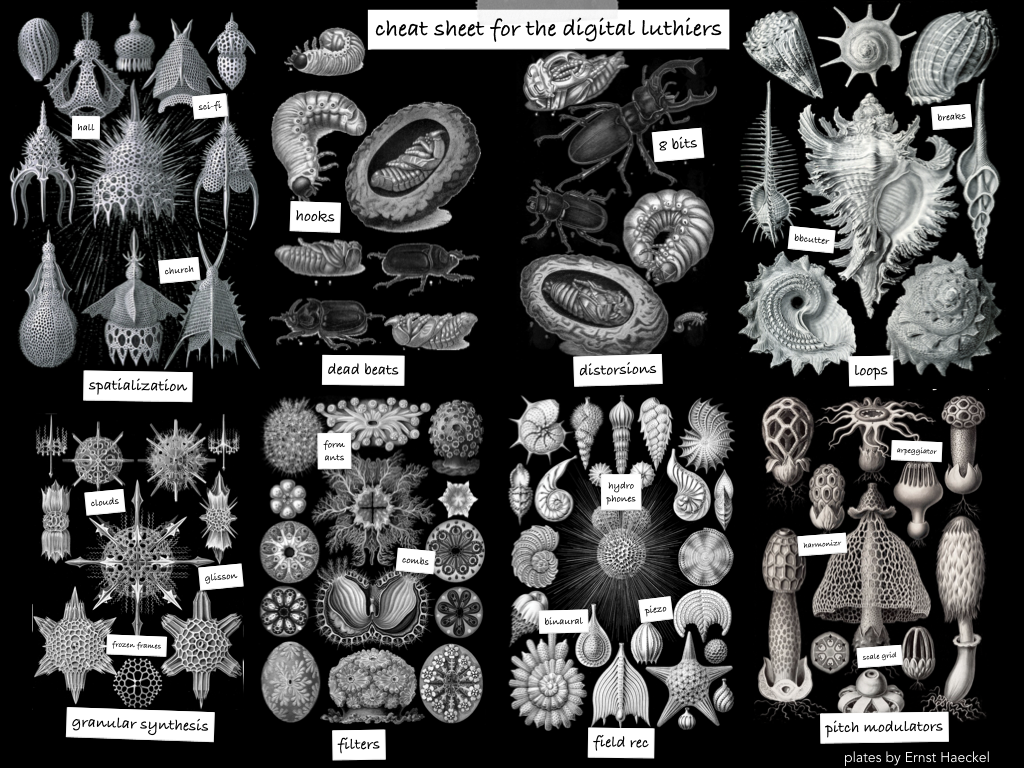
\includegraphics[width=\textwidth]{gfx/02_ephemeral/Bestiaire.png}
	\caption{Entomologie musicale}
	\label{fig:ephemeral:entomologie}
\end{figure}
%-------------------------- Figure : Entomologie ----------------------------------
\noindent Les \glspl{DMI} s'apparentent ainsi à des vaisseaux hétérogènes, chargés de souvenirs de nos expériences d'interprétation, de composition ou de fabrication d'instruments. Les sons que nous recueillons, les algorithmes de synthèse que nous développons (ou téléchargeons), les paramètres que nous ajustons, les recettes de cuisine et les fonctions de transfert que nous élaborons avec soin, contribuent à l'évolution d'un répertoire personnel où se cristallisent des instances éphémères. Thor Magnusson a proposé le terme ``d'outil épistémique'' pour décrire les \glspl{DMI} comme \iquote{un outil conçu avec un tel degré de pertinence symbolique qu'il devient un système de connaissance et de pensée dans ses propres termes} \cite{magnusson_epistemic_2009}.\\
\indent Ainsi, les \glspl{DMI} se présentent comme des assemblages évolutifs de ces matériaux enregistrés et impliquent souvent des activités qui ne sont généralement pas associées à la pratique instrumentale, comme la gestion de fichiers, le versionnage du code, le recensement de ressources en ligne ou l'organisation de banques de sons, afin de pouvoir réunir ces ressources aussi rapidement que possible pour la performance.\\
\indent Il est remarquable que les possibilités de duplication et de diffusion offertes par les médias numériques et Internet n'aient pas conduit à la standardisation des instruments ; les \glspl{DMI} sont souvent très personnels et singuliers.

\section{Conclusion}

\noindent Ce chapitre a permis de présenter les \glspl{DMI} à travers la notion d'assemblage éphémère qui les caractérise, en la considérant non pas seulement comme un problème, mais comme une modalité intrinsèque de leur ontologie. Loin d'exclure leur longévité, elle éclaire au contraire la conception technique des environnements propices à leur développement et à leur durabilité.\\
\indent L'éphémérité des outils n'empêche pas la production de musique passionnantes, ni la réalisation de performances musicales captivantes. Au contraire, elle peut à la fois favoriser l'adaptation des assemblages musicaux à des contextes essentiellement éphémères et défier la capacité de l'être humain à répondre à un dispositif musical fugace et indompté.\\
\indent Il y a un millénaire, l'émergence de la notation musicale a entraîné une multiplication du nombre de compositions, dont un grand nombre connurent une vie éphémère en terme de performances. Le numérique nous amène peut-être aujourd'hui à une situation similaire en ce qui concerne l'instrument : la possibilité de le ``noter'' sous forme de code donne lieu à une multiplication du nombre de nouveaux instruments. En mettant cette révolution en perspective de celle que fût l'écriture musicale il y a un millénaire, et de qu'elle permit en terme de création de forme (de l'\textit{ars antiqua} à l'écriture symphonique), on peut espérer que la \textit{notation instrumentale} soit aussi fertile.\\
\indent En fin de compte, les œuvres musicales (et les instruments) semblent trouver leur chemin, qu'on les appelle ``répertoire classique'', ``standard de jazz'' ou ``airs traditionnels'', mais ce n'est pas tant la pérennité de leur notation qui les fait survivre --~elles pourraient rester \textit{lettre morte}~--, que l'intérêt que leur portent les vivants, qui soutiennent par leurs soins et leur travail celles qu'ils reconnaissent comme chefs-d'œuvre. Elles peuvent résister à l'épreuve du temps en étant dispersées, distribuées, transformées, recomposées, réinterprétées ou même renommées, par tous ceux qui y attacheront de l'importance. Ce soin attentionné, mû par notre désir de musique, appartient probablement à la partie de notre mémoire que nous ne pouvons pas externaliser dans un outil et qui redéfinit la tradition et la préservation en dehors du cadre technologique.\\
\indent Dans le sable évoqué par Michel Chion, nous pouvons voir une autre métaphore intéressante pour les \glspl{DMI}: à l'origine, le sable est une roche, qui s'est progressivement atomisée, fragmentée en particules infimes. La même chose semble s'être produite pour les instruments de musique, atomisés en petits modules numériques. Nous pouvons jouer avec le sable comme un matériau fluide, ou lui ajouter de l'eau, voire du ciment, pour lui donner une forme concrète.\\
\indent Si les technologies numériques arrivent un jour à maturité, nous pourrons peut-être compter sur des instruments numériques stables et durables. Dans ce cas, et faisant suite à la prémonition de Garsault, il ne faudra pas oublier de classer tous les instruments éphémères qui les ont précédés dans la catégorie des \iquote{instruments hors d'usage, mais qui peuvent revenir}.


%\section{extra material}

% Thor Magnusson in Sonic Writing (p12) : Anyone who plays a musical instrument will be familiar with the special moment when a new instrument is picked and its ergodynamics studied through play. (footnote : we often change our instruments during performance : we retune string instruments, change effect settings in electronics, and the \textit{whole point} of live coding is to create and redefine the instrument during play). This experience of ergodynamics recognises that an instrument is an object that never rests, or enter a period of stasis: that every time we pick it up there are new things to discover, new patterns our fingers know, because we have changed, the instrument has changed, and so has the whole world itself — the general performance context.

% De même que l'histoire a connu une importance prépondérante des musiques traditionnelles\footnote{Les musiques trad existent toujours, et d'une certaine manière, un standard de jazz est une musique traditionnelle}, à une époque où l'absence d'écriture et d'enregistrement rendait cette tradition nécessaire à la répétition, la période allant du Moyen-Age à l'époque contemporaine a été marqué par la prépondérance d'instruments traditionnels, à défaut de pouvoir agencer ces instruments de manière plus souple, comme l'a permis l'écriture pour la composition musicale. La possibilité de ``noter'' ces instruments sous forme de grammes, ainsi que les gestes ne rend plus nécessaire l'existence de tradition instrumentale, ou plutôt, rend plus que jamais possible l'invention instrumentale.

% De même que l'on peut travailler une partition et devenir expert dans son interprétation, on peut travailler un instrument pour en devenir expert et travailler les différentes compositions pour cet instrument. On peut aujourd'hui travailler le geste (et l'écoute!) et en devenir expert pour jouer les différents instruments qui s'offrent à ces gestes. % INCLUDE: introduction
% !TEX root = ../thesis-example.tex
%
\chapter{L'instrument et le geste}
\label{ch:gesture}

\cleanchapterquote{La percussion de ce pseudo-gong est illlusoire :\\
rien ne tape sur rien dans l’ordinateur.\\
Schumann qualifiait le legato au piano\\
de ``trompe-l’oreille'' : la musique est aussi un art\\
du mirage, de l’illusion.}{Jean-Claude Risset}{Discours invité aux JIM 2010 \cite{risset_propos_2010}}

Proprioception et schema corporels (cf. Miranda unconventional computing)

%L'expression musicale a été contrainte (et non ``prisonnière'', car la contrainte peut être fertile) par la relation causale entre le geste d'excitation et le son produit par l'instrument dans les lutheries acoustiques.

\noindent Poursuivant des évolutions organologiques latentes, telles que présentées dans la section \ref{sec:ephemerality:landscape}, les \glspl{DMI} finissent d'opérer un découplage énergétique, une ``dislocation du contrôle'' (\textit{control dislocation} \cite{miranda_new_2006}), rompant avec plus de 35.000 ans de tradition musicale \cite{conard_new_2009} et avec l'unité de temps, de lieu et d'action —définie en règle par le théâtre classique, mais qui reflète la relation qui existait entre l'auditeur et le phénomène sonore, comme le rappelle Hugues Genevois dans \cite{cance_what_2012}.\\
\indent L'introduction de la mémoire et de la computation numérique permet une re-programmation complète de l'interaction, rendant leur fonctionnement à la fois complexe et cryptique. Cet aspect peut se révéler être un inconvénient, dans la mesure où il prive le public d’une lecture possible de la performance musicale. Cela peut cependant s’avérer être un avantage, si l'on considère que la performance musicale comporte une part scénographique dans laquelle l’illusion a toute sa place.\\
\indent Nous allons voir dans ce chapitre comment le geste instrumental s'en trouve affecté, par un examen critique des catégories gestuelles déjà proposées, la proposition de nouvelles catégories prenant en compte l'aspect subversif de l'art musical et les conséquences que nous pouvons en tirer en termes de conceptions des \glspl{DMI}.


\section{Introduction : L'étude du geste en musique}

\noindent Si l'étude du rythme et plus encore, des hauteurs, a été particulièrement importante dans la culture classique occidentale, l'étude du geste a longtemps été négligée voire méprisée, comme le rapporte Jean-Marc Warszawski\footnote{Conférence La musique et le geste : \url{https://www.musicologie.org/18/la_musique_et_le_geste.html}.}: \iquote{La tradition savante occidentale, grâce à l'écriture, dématérialise le geste créatif musicien, et impose une ligne de démarcation ente musique écrite et non écrite, en quelque sorte une frontière entre le primitif et le civilisé.}\\
\indent Peut-être faut-il également y voir une autre raison : le geste ne se laisse pas aussi facilement mesurer, encore moins définir, que la hauteur. Si cette dernière peut se  réduire en première approximation à une grandeur physique mesurable --~sa fréquence fondamentale\footnote{La perception de la hauteur est évidemment plus complexe que l'évalutation de la fondamentale et un des sujets d'étude de la psycho-acoustique, voir notamment les travaux de Michèle Castellengo \cite{castellengo_ecoute_2015}. L'écriture musicale classique s'est toutefois largement construite sur cette réduction, que Robert Francès nomme ``abstraction notale'' \cite{frances_perception_1984}.}, le geste ne se laisse pas aussi facilement réduire à une mesure. Il entraine depuis sa production jusqu'à sa réception toute la complexité du vivant : sa multidimensionalité, son instabilité, sa relativité, sa combinatoire, et l'ensemble de ses aspects culturels... (TODO : développer et/ou enlever les pointillés)\\
\indent L'étude du geste se développe dans le courant du \siecle{19}~siècle, sous l'effet de la révolution industrielle, de l'étude mécanique du mouvement et la création de conservatoires qui développent des techniques d'apprentissage où le geste est pris en compte\footnote{Voir en particulier la collection rassemblée sur le site de la Bibliothèque Nationale de France: \url{https://gallica.bnf.fr/html/und/partitions/oeuvres-theoriques-et-pedagogiques}. L'intérêt pour le geste à cette période de développement industriel donne lieu par ailleurs à l'invention d'étonnants systèmes mécaniques servant à guider, contraindre et fortifier les gestes, en particulier pour le piano, tels que le ``chiroplaste'' ou le ``dactylion'', mais qui s'avèrent être davantage des instruments de torture, endommageant parfois les mains de manière irréversible.}. L'étude du geste a progressivement gagné en importance, d'une part avec l'émergence de l'anthropologie au début du \siecle{20}~siècle, et d'autre part suite à l'explosion des technologies de télécommunication, lorsque sa compréhension et sa modélisation sont devenues nécessaires pour le développement des \gls{IHM} dans la seconde moitié du siècle, jusqu'à devenir un domaine d'étude à part entière, les \textit{gesture studies}, soutenue notamment par l'\gls{ISGS} créée en 2002.\\
\indent Dans le domaine de la musique, c'est l'arrivée du ``temps-réel'' et l'émergence des \glspl{DMI} dans les années 1980, qui entraine la parution croissante d'articles traitant de la question du geste instrumental. Au tournant du siècle (du millénaire), le geste devient un objet d'étude majeur dans le domaine de l'informatique musicale, se traduisant notamment par la parution d'ouvrages collectifs dédiés\footnote{Voir en particulier : \cite{genevois_les_1999}, \cite{wanderley_trends_2000} et \cite{godoy_musical_2010}}, ainsi par que l'apparition de la conférence \gls{NIME} en 2001, qui lui accorde une place importante.\\
\indent Plusieurs projets de recherche interdisciplinaires ont également été menés, comme le projet ConGAS\footnote{``Gesture Controlled Audio Systems'', projet financé entre 2003 et 2007 dans le cadre de la Coopération Européenne en Sciences et Technologies (COST Action 287)}, ou plus récemment le projet Gemme\footnote{``Geste musical : modèles et expériences'', projet de recherche financé par l'ANR de 2012 à 2016, dont un carnet de recherche en ligne est disponible : \url{https://geste.hypotheses.org/gemme}} et la chaire thématique pluridisciplinaire GeAcMus\footnote{La chaire``Geste - Acoustique - Musique'' a été créée en 2015 à Sorbonne Université \url{http://www.sorbonne-universites.fr/actions/recherche/chaires-thematiques/geacmus.html}} créée à Sorbonne-Université.

\extra{Le terme Gesture est utilisé dans 62\% des articles publiés à NIME (cf. Jensenius paper : To Gesture or Not? An Analysis of Terminology in NIME Proceedings 2001–2013) <= update this}


\section{Geste instrumental et geste musical}

\subsection{La musique et ses instruments}

\noindent La définition du geste musical pose le double problème de définir ce qu'on entend par ``geste'' et par ``musique''. Pour ce qui est de la musique, j'adopterai ici la définition proposée par Christopher Small, non pas du \textit{nom} ``musique'', mais du \textit{verbe} qu'il invente : ``musiquer'' \cite{small_musicking:_1998}:
\iquote{Musiquer, c'est participer, à quelque titre que ce soit, à une performance musicale, que ce soit en jouant, en écoutant, en répétant ou en pratiquant, en fournissant du matériel pour la performance (ce qu'on appelle ``composer''), ou en dansant. Nous pourrions même parfois en étendre le sens à ce que font la personne qui prend les billets à l'entrée, les gros bras qui déplacent le piano et les tambours, les roadies qui installent les instruments et font les balances ou les personnes qui nettoient après que tout le monde soit parti. Ils contribuent tous, eux aussi, à la nature de l'événement qu'est une performance musicale.}\\
\indent Si j'adopte ce néologisme, ce n'est pas pour l'exhaustivité que semble conférer une définition aussi large mais essentiellement pour deux raisons: la première est le choix d'utiliser un verbe plutôt qu'un nom, c'est-à-dire d'identifier une pratique plutôt qu'un objet, ce qui dans le cas de la performance musicale semble mieux adapté. La deuxième raison est liée au contexte technico-culturel dans lequel ces pratiques s'inscrivent: la reconfiguration des modes de production et de réception de la musique\footnote{voir à ce sujet l'ouvrage de Paul Théberge \cite{theberge_any_1997}} qu'ont entrainée les évolutions technologiques du \siecle{20}~siècle ont rendu poreuses les frontières entre les différentes pratiques liées à la création musicale. Je restreindrai toutefois le champ de cette définition aux pratiques qui gravitent directement autour de l'instrument de musique, tel que présenté dans le chapitre précédent.\\
\indent Partant de cette définition et reprenant une proposition d'Hugues Genevois \cite{genevois_geste_1999}, on peut distinguer plusieurs phases au cours desquelles se manifeste un geste musical :

\vspace{-1em}
\begin{itemize}[noitemsep]
\item \textbf{la composition} : la production de structure musicales hors-temps de leur rendu sonore;
\item \textbf{la lutherie} : la réalisation de l'instrument et sa préparation pour le jeu;
\item \textbf{la performance} : le jeu instrumental qui produit, modifie, mélange, dans le temps même de l'écoute, la matière sonore, les gestes de l'instrumentiste, du chef, de l'ingénieur du son;
\item \textbf{l'écoute} : qui construit l'intelligibilité de notre environnement sonore et se mobilise sans répit pour en garantir la cohérence;
\item \textbf{la pédagogie} : durant laquelle la complexité du geste musical se transmet progressivement, en étant guidée, soutenue, encouragée, critiquée, en se pratiquant parfois sous la forme d'exercices idiomatiques et systématiques (e.g. faire ses gammes), et à travers des allers-retours entre performance et écoute.
\end{itemize}

\noindent Dans la pratique, ces différents gestes se superposent souvent mais pourront se traduire par différentes formes de configurations instrumentales, adaptées aux spécificités de chaque situation (TODO : développer ou renvoyer à une section ultérieure qui développe).

\subsection{Définition(s) du geste}

\noindent Dans sa définition générale, le Littré, le Larousse ou le dictionnaire de l'Académie Française s'accordent à le définir comme \iquote{un mouvement du corps, principalement de la main, des bras, de la tête, porteur de sens ou non} (Larousse).

\noindent \textbf{aspects phénoménologiques} Un premier aspect du geste est sa nature de mouvement, son déploiement spatial et temporel, dont les qualités spatiales, cinématiques, cinétiques, synchroniques, fréquentielles, balistiques (...) abstraites font écho à la mémoire de tous les mouvements dont nous faisons l'expérience: battements, ondulations, chutes, éclosions, envols, éruptions, roulements, contractions, extensions, sursauts... Le geste possède une force expressive, en dehors de toute interprétation sémiotique, génératrice de sensations dont la logique ne peut être décrite que par la métaphore\footnote{C'est en particulier l'entreprise de Gaston Bachelard dans son travail de ``phénoménologie de l'imagination'' \cite{bachelard_air_1943}}.\\
\indent Ce mouvement est l'expression même du vivant et il reflète à la fois la relation du corps à son environnement externe (force de gravité et cinétique, contournement d'obstacles, frictions sur les matériaux, contraintes formelles chorégraphiques...) et l'expression des mouvements internes du corps (vigueur ou mollesse, souple ou crispé, émotion se traduisant par des gestes tels que haussement d'épaule, sursaut de surprise, grimaces diverses, etc.). La maitrise de ces mouvements est un aspect fondamental de la danse qui, comme la musique le fait avec le son, met en œuvre le corps dans des intensités, des rythmes, des trajectoires. Si les gestes de la danse ne sont pas \textit{a priori} instrumentaux, les \glspl{DMI} rendent plus que jamais possible leur utilisation à des fins d'interaction musicale, comme nous le verrons plus loin (cf. notamment \cite{bevilacqua_gesture_2011, alaoui_movement_2012, silang_maranan_designing_2014, hsueh_understanding_2019}.)

\noindent \textbf{aspects sémiotiques} Un deuxième aspect du geste est indiqué par le curieux épithète de la définition précédente : ``porteur de sens ou non''. S'il a semblé utile d'évoquer une qualité potentiellement absente, c'est précisément parce les différentes définitions qu'on donne du geste dépendent en partie de cet aspect sémiotique, qui reste soumis à une interprétation subjective et contextuelle dans un système de valeurs. Les significations d'un geste peuvent en effet être attribuées par l'auteur du geste ou bien par celui ou celle qui observe ce geste, sans qu'il n'y ait nécessairement de correspondance, ni en terme de signification, ni sur la part du mouvement considérée signifiante. La signification d'un geste peut également être attribuée par la machine, en particulier dans les systèmes d'apprentissage, comme nous le verrons plus loin.

\noindent \textbf{aspects ergotiques} Une autre définition du geste relève sa dimension manipulative : \iquote{Manière de mouvoir le corps, les membres et, en particulier, manière de mouvoir les mains dans un but de préhension, de manipulation} (Larousse). Cette définition met l'accent sur la relation possible entre le geste et un objet, un outil, un instrument et s'applique par conséquence particulièrement bien à la situation instrumentale. C'est sur cet aspect que se concentre notamment les typologies gestuelles proposées par Claude Cadoz que nous discuterons plus loin.

\noindent \textbf{aspects (dia)grammatiques} Enfin, si le geste \textit{ex-prime} (du latin \textit{ex-premo} : ``faire sortir en pressant'') des mouvements internes du corps, il \textit{im-prime} et laisse une trace dans la matière, dans la machine, dans les esprits. C'est parfois cette trace résultante qu'on nomme geste, par métonymie et analogie avec les qualités de mouvement qui sont à son origine, lorsqu'on parle par exemple du \textit{geste de composition}. Les capacités des machines à enregistrer le geste dans sa dynamique --~auparavant éphémère et seulement visible sous la forme de traces statiques: littérature, peinture, partition~-- confèrent à cet aspect \textit{diagrammatique} du geste une importance particulière à l'époque de sa reproductibilité technique\footnote{L'expression utilisée ici revoie bien évidemment à l'œuvre éponyme de Walter Benjamin\cite{benjamin_loeuvre_2013}}, qu'il nous faut souligner et qui sera analysée en dernier lieu.

%--------------------------------------------

La fonction sémiotique du geste a occupé une grande place dans son étude au \siecle{20}~siècle, notamment sous l'influence conjointe de l'anthropologie naissante, analysant les systèmes d'interaction sociale de différentes cultures \footnote{Adam Kendon, Marcel Jousse, Bernard Koechlin, André Leroi-Gourhan...} mais aussi de l'explosion de la télécommunication et des recherches scientifiques qui ont accompagné cette révolution technologique.

L'influence de la théorie de l'information de Claude Shannon (cf. figure TODO), en particulier, a contribué à envisager le geste, dans une perspective communicationnelle. Les analyses qui en résultent s'inscrivaient alors, plus ou moins explicitement, dans une perspective d'encodage efficace, en extrayant l'information qu'il contient, et par inférence, sa signification supposée.

Cette influence est particulièrement sensible dans l'école Anglo-Saxonne, centrée sur les figures de Adam Kendon et David McNeil, qui confèrent au geste une signification préalable à son existence. D'après McNeil, \iquote{(...) le geste est créé par le locuteur comme une matérialisation du sens'' \iquote{(...) a gesture does not represent at all; the gesture is created by the speaker as a materialization of meaning. }, \cite{mcneill_gesture_2005}}

A l'opposé, l'approche phénoménologique adopte un autre point de vue en conférant au geste un statut pré-sémiotique et un pouvoir créatif et expressif.
Guerino Mazzola : \iquote{Gestures are dialogical, live in presence, are circular, elastic, are presemiotic, and are as such already differentiated (being gestural can be ramified into different types).} \cite{mazzola_topos_2018}, p. 59 (852)

Le geste peut être porteur d'un sens préalable (McNeil) ou d'un sens 

D'une certaine manière, ces deux approches se placent de part et d'autre du processus de communication, du point de vue de l'auteur du geste (Gesture and thoughts, chez McNeil) et de son observateur (Phénoménologie de la perception).

Le geste \textit{exprime} (du latin \textit{ex-premo} : ``faire sortir en pressant'') quelque chose, mais n'a pas nécessairement une signification.


Pour autant, on se rend bien compte que tous les mouvements du corps ne sont pas nécessairement en permanence associés à l'idée de geste. Dans le cadre d'une activité spécifique telle que la pratique musicale, impliquant la participation active de l'individu, la plupart des études (todo:mettre plusieurs ref) sur le geste s'accordent à le définir comme l'association d'un mouvement et d'une intention.

\iquote{Le geste doit être défini comme un mouvement intentionnel plus ou moins complexe, orienté vers un but déterminé qui lui donne un sens individuel, social ou historique.} \cite{imberty_mouvement_2013}

\noindent L'intention gestuelle peut être envisagée selon différent points de vue, selon que son étude porte sur sa fonction sémiotique (le geste-signe), ergotique (le geste-action), épistémique (le geste de perception).\\
\indent La notion de geste est également utilisée pour décrire des formes indirectement liées au mouvement physique, telles que le ``geste de composition'', en transposant par analogie le mouvement et l'intention le caractérisant. On voit donc que la question de l'intention soulève des questions esthétiques voire politiques : l'inscription de la performance musicale dans la vie sociale et culturelle pose la question de la place du geste dans un système de valeurs spécifique. En particulier, l'époque postmoderne est caractérisée par un art qui attribue davantage d'importance à \textit{l'intérêt} du geste pris dans un contexte \textit{expérimental}, qu'à sa \textit{beauté}, prise dans un contexte \textit{normatif} classique.

\indent Enfin, en tant que phénomène de transfert d'énergie et d'information, le geste pourra être évaluée différemment selon qu'on se place du point de vue de sa production ou de celui de sa réception. 

La ``geste'' en musique a ainsi été utilisée pour décrire différents aspects de la relation qu'entretiennent le mouvement, l'instrument, l'intention, la morphologie et la signification du son ou encore les formes d'écritures compositionnelles. L'instrument de musique se trouvant à la croisée de ces différents chemins, la notion de ``geste instrumental'' a souvent été liée voire confondue avec celle de ``geste musical''. 

La relation entre musique et mouvement du corps dépasse le domaine de l'interaction instrumentale. Par exemple, les mouvements de la danse, s'il peuvent être en corrélation avec la musique, ne sont pas a priori des gestes instrumentaux. Cependant, si les mouvements du danseur sont captés et interagissent avec la production du son — ce qui est particulièrement rendu possible avec les nouvelles technologies, alors ils peuvent être envisagés comme relevant du geste instrumental.

Le geste instrumental parait au premier abord plus simple que le geste musical, en ce qu'il semble davantage possible de le décrire à travers une approche purement fonctionnelle de sa mécanique. 

Dès 1995, Todd Winkler propose de repenser le geste instrumental dans les \glspl{DMI} en proposant des contraintes et des idiomes libérés du modèle de l'instrument acoustique \cite{winkler_making_1995}. Sa formulation de cette problématique est intéressante en ce qu'elle envisage déjà la sonorité des gestes au-delà du modèle acoustique excitation/résonance (``le son du claquement d'une seule main''). Cependant, ses propositions reflètent son attachement au paradigme physique et à la corrélation entre l'énergie du geste et du son : \iquote{Qu'est ce que la musique des doigts ? Qu'est ce que la musique de course ? Quel \textit{est} le son d'\textit{une seule} main qui claque ? On peut répondre à ces questions en permettant à la physicalité du mouvement d'avoir un impact sur le matériel et les processus musicaux. Ces relations peuvent être établies en considérant le corps et l'espace comme des instruments de musique, libérés des relations dans les instruments acoustiques, mais avec des contraintes similaires qui peuvent donner du caractère au son par des mouvements idiomatiques.}\footnote{\iquote{What is finger music? What is running music? What \textit{is} the sound of \textit{one} hand clapping? These questions may be answered by allowing the physicality of movement to impact on musical material and processes. These relationships may be established by viewing the body and space as musical instruments, free from the associations of acoustic instruments, but with similar limitations that can lend character to sound through idiomatic movements.}}





% Jensenius in Musical Gesture : "Based on the above viewpoints, it seems straightforward to define musical gesture as an action pattern that produces music, is encoded in music, or is made in response to music. Qualifications can be added to the term musical gesture whenever needed to avoid misunderstandings. For example, one can speak about sound-producing gestures, sound-modifying gestures, sound-accompanying gestures, sonic gestures, playing gestures, and so on."


% Par ailleurs, certains auteurs font une distinction entre ``geste avec contact'' et ``geste sans contact''. Je propose d'envisager cet aspect d'une manière généralisée en parlant du retour gestuel dans le ``geste interactif''. Cette interaction existe toujours, mais avec plus ou moins d'importance, et plus ou moins de simultanéité. Ce retour peut être de nature physique, vibratoire, acoustique mais également visuel ou kinesthésique.



Guerino Mazzola : \iquote{Gestures are dialogical, live in presence, are circular, elastic, are presemiotic, and are as such already differentiated (being gestural can be ramified into different types).} \cite{mazzola_topos_2018}, p. 59 (852)

Le geste \textit{exprime} (i.e. du latin ex-premo : ``faire sortir en pressant'') quelque chose, mais n'a pas nécessairement une signification.


Le geste + intention ? => le geste ne passe pas nécessairement pas un dessein connu d'avance, il se produit aussi en réaction à la vivacité de la musique produite dans une circularité qui ne laisse pas de place à la mentalisation de l'instant (flow).

%-------------------------------------------
\subsection{Spécificités des DMIs}

\noindent Dans le contexte particulier des lutheries numériques, un certain nombre de problèmes se posent par rapport au geste instrumental sur les instruments acoustiques, liés à des spécificités du numérique que nous avons déjà en partie évoqué dans le chapitre précédent\footnote{De manière plus globale et sociologique, les révolutions technologiques électroniques ont également modifiés les modes de production et de réception de la musique à l'échelle industrielle, entrainant d'autre conséquences que celles listées ci-après, mais qui dépasse le sujet que nous traitons ici. Je renvoie pour ces questions là au travail de TODO : Bacot, Collins, Auslander, Rebecca Bennett, etc.}.

\vspace{-1em}
\begin{itemize}[noitemsep]
\item \textbf{le découplage énergétique} : ce découplage est la différence la plus saillante par rapport aux lutheries acoustiques. Certains de ses aspects sont déjà présents dans les instruments électriques et électroniques, mais l'informatique numérique ajoute un découplage de plus: les signaux (gestuels, sonores) n'y existent plus sous forme analogique et se présentent sous la forme de représentations numériques du signal, c'est-à-dire encodés dans un alphabet.
\item \textbf{la mémoire et le temps différé}: si le terme de ``temps réel'' est abondemment utilisé quand on parle des \glspl{DMI}, il ne faut pas oublier que l'informatique introduit avant tout le temps la possiblité du temps différé, de l'enregistrement exploitable dans le futur.
\item \textbf{la computation} : le traitement algorithmique permet --~ou impose~-- une reconfiguration permanente des modèles et des représentations, qui entraine une instabilité, un métamorphisme des relations entre les données.
\end{itemize}

TODO : intégrer ici le fait que les DMIs ne sont pas des IHMs ?



%%%%%%%%%%%%%%%%%%%%%%%%%%%%%%%%%%%%%%%%%%%%%%%%%%%%%%%%%%%%%%%%%%%%
\section{Limites d'une analyse des DMI comme IHM}
\label{sec:gesture:limitesIHM}

\subsection{La scène et le laboratoire}
Catégories gestuelles établies via une analyse ``de laboratoire'', qui visent à étudier les phénomènes pris isolément, hors du contexte de performance. Il en est ainsi de l'analyse Schaefferienne et de l'écoute réduite, qui bien que très utile pour la compréhension des sons autant que pour le compositeur qui veut les utiliser comme un matériau plastique, ne reflète pas une situation généralisable au public d'un concert.

Un certain nombre de critères ont ainsi été proposés pour améliorer le design des DMIs, souvent en prenant comme modèle l'instrument acoustique classique, tant en terme d'affordance de l'objet, qu'en terme de relation socio-culturelle (todo:trouver plus précis que socio-culturel) pour le cadre qu'il offre à l'instrumentiste et au public (notamment, l'instrument est sur scène, entre les mains de l'instrumentiste, la relation geste-son est lisibile, sa palette sonore est connue d'avance par le public, etc.).
Au delà d'un effet diligence\footnote{todo expliquer}, le désir de retrouver les qualités d'affordance des instruments classiques s'explique par la riche histoire instrumentale dont on souhaite tirer profit pour le design de nouveaux instruments. La tâche s'avère cependant complexe et difficile et parallèlement, les lutheries numériques se sont développées de manière empirique, ``sauvage''\footnote{cf. Max Vandervorst, John Bowers, etc.} en s'adaptant au medium tel qu'il se présente, et en inventant de nouveaux gestes et sans forcément s'inscrire dans un contexte de performance similaire à celui des instruments classiques (instrument hors scène, ou invisible, relation gestuelle et timbre mé-connus, etc.)

%-------------------------------------------
\subsection{Nouvelles IHM, nouveaux gestes}

Notons que dans leur classification, Cadoz et Wanderley \cite{todo} définissent le geste instrumental comme un geste \iquote{appliqué à un objet matériel et en interaction physique avec lui}, ajoutant que \iquote{les gestes nus (empty-handed gestures) ne sont pas des gestes instrumentaux pour la raison qu'il ne possède qu'une fonction sémiotique}.

Depuis, le nombre de capteurs permettant une interaction sans contact physique n'a cessé d'augmenter et de se démocratiser : caméras vidéos, caméras 3D (e.g. kinect, leap motion), capteurs de distance à infra-rouge ou ultra-sons, capteurs photosensibles, gyroscopes et accéléromètres... entrainant une croissance proportionnelle du nombre de DMIs recourant à des gestes sans contact physique.

On perçoit évidemment les limites de cette notion de contact physique, quand il s'agit d'instruments comme le theremin, ou quand des capteurs sans contacts tels que les capteurs de distance par ultra-son ou infra-rouge, les caméras vidéo, les kinect\footnote{interface conçue par Microsoft, qui s'apparente à une caméra fournissant, en plus d'une image vidéo classique, une carte de profondeur de l'image captée.}, leap-motion\footnote{interface conçue par Microsoft, qui s'apparente à une caméra fournissant, en plus d'une image vidéo classique, une carte de profondeur de l'image captée.} et autres radars... Le \textit{geste nu} s'apparente dans ce cas à un geste ergotique (si toutefois cette notion de geste ergotique conserve un sens dans les DMI).

Dans le cas des \glspl{DMI}, la relation entre le geste et le son se pose d'une manière précisément opposée : la relation entre le ``geste de production du son'' et le son n'y est pas causale a priori.

%-------------------------------------------
\subsection{Geste produit, capté, perçu}

cf Benford \cite{benford_performing_2010}

Dans le domaine des IHM, peu d'importance est accordée au geste en dehors de son interaction directe avec l'ordinateur, comme le rapporte Jensenius (Musical Gesture):
\iquote{A gesture is a motion of the body that contains information. Waving goodbye is a gesture. Pressing a key on a keyboard is not a gesture because the motion of a finger on its way to hitting a key is neither observed nor significant. All that matters is which key was pressed}(p. 310)\cite{kurtenbach_art_1990}

Pourtant comme le rappelle Richard Leppert dans \cite{leppert_sight_1993} (cité par \cite{iazzetta_meaning_2000}) souligne à quel point la nature intangible du son et de la musique est polarisée par l'expérience visuelle :
\begin{quotation}
Precisely because musical sound is abstract, intangible, and ethereal [...] the visual experience of its production is crucial to both musicians and audience alike for locating and communicating the place of music and musical sound within society and culture. [...] Music, despite its phenomenological sonoric ethereality, is an embodied practice, like dance and theater." 
\end{quotation}

Il faut également noter que si la réalisation d'un geste technique sur une interface est orientée vers l'efficacité pour la réalisation d'une tâche, \cite{ryan_remarks_1991}

Un geste musical ne consistera donc pas prioritairement à chercher une efficacité pour accomplir une tâche mais 



\textbf{Différence entre geste effectué et geste capté} : un son électroacoustique, par exemple une figure de ``delta'', pourra ainsi avec un même geste de balaiement de la main, et une même interface de captation (e.g. un simple slider), être déclenchée via un seuillage de l'entrée qui déclenche un sample, être produit de manière continue, via un scrub du sample, pourra avoir son intensité sonore fonction de la vitesse du geste ou pas, etc. On voit que pour un même geste, un même son (échantillonné), et un même capteur, les possibilités de relations entre le geste et le son sont multiples. Le pré-geste hors contact avec l'instrument pourra être capté ou non selon le capteur. (e.g. leap motion)



%-------------------------------------------
\subsection{Les musiciens \emph{ne sont pas} des utilisateurs d'instruments}

Un autre biais de l'approche fonctionnelle des \gls{IHM} est lié au fait que l'interaction est souvent définie par la perspective d'une tâche que l'utilisateur doit accomplir. Ce contexte écologique a contribué au développement de tout un champ d'étude dans le domaine des IHM: les \textit{user studies}, transposé dans le domaine de l'ingénierie industrielle sous le nom d'``Experience Utilisateur''\footnote{En abrégé : UX pour User eXperience; le métier de ``UX designer'' étant désormais très répandu dans le domaine du développement logiciel mais également appliqué à d'autres domaines tels que la grande consommation.}.
%---- Figure : Einarsson sculpture ---------
\begin{figure}[!htbp]
	\captionsetup{format=plain}%
	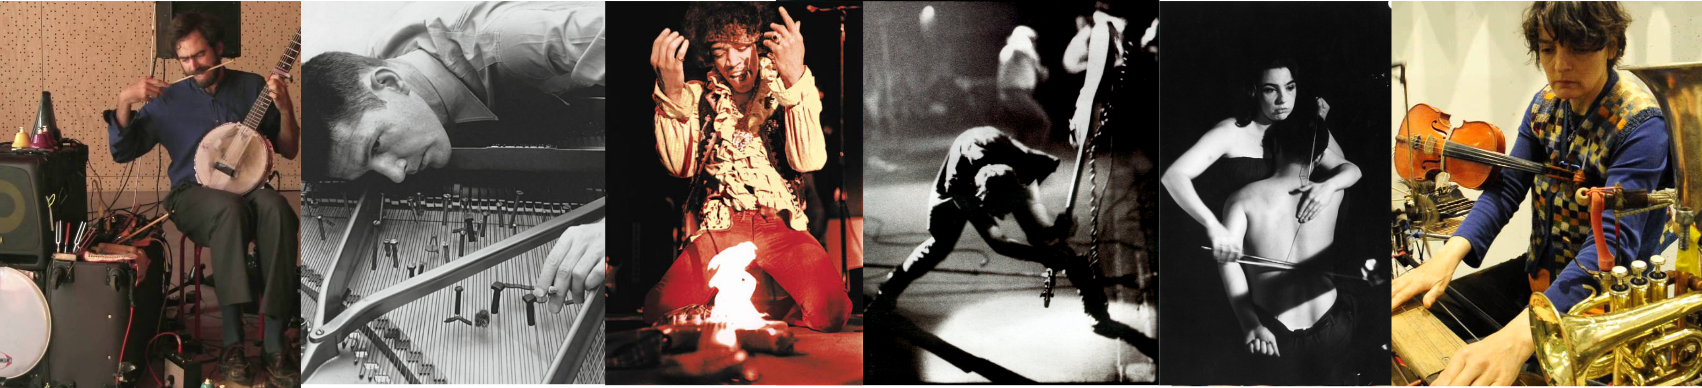
\includegraphics[width=\textwidth]{gfx/03_gesture/instrumentabusers.png}
	\caption[Les instrument ne sont pas des interfaces utilisateur]{Les instrument ne sont pas des interfaces utilisateur. De gauche à droite : Thomas Bonvallet, John Cage, Jimi Hendrix, Paul Simonon, Charlotte Moorman, Sarah Kenchington}
	\label{fig:gesture:abusers}
\end{figure}
%---- Figure : Einarsson sculpture ---------
\noindent Or dans une performance musicale vivante, cette situation n'existe pas. Le musicien ne saurait être défini comme ``l'utilisateur de son instrument''(figure \ref{fig:gesture:abusers}), pas plus que son instrument comme une ``interface utilisateur''. Les musiciens cherchent bien souvent à produire quelque chose à la limite des possiblités de leur instrument\footnote{cf. interview de Nicolas Bernier désignant ``l'infini des possibles'' comme principale motivation l'ayant amené à utiliser les instruments électro-acoustiques.}. Que cela soit le contre fa de la Reine de la Nuit, les partitions impossibles de Brian Ferneyhough, les pianos préparé de John Cage, le scratch sur les platines vinyle ou les mises en larsen de table de mixage de la scène Onkyokei, les exemples abondent dans l'histoire de la musique qui font preuve d'une démarche allant dans l'outrepassement des possibilités instrumentales lors du jeu musical. Dans une conversation durant la dernière conférence NIME, Paul Stapleton utilisait ironiquement le terme \textit{interface abusers} pour souligner l'erreur du terme \textit{interface users}. \footnote{Un exemple significatif de cette différence entre usage et abus de l'instrument est la réduction de la hauteur dans le format MIDI à un paramètres entier borné entre 0 et 127 pour contrôler la hauteur—ce qui excède déjà la tessiture du piano à 88 touches. Les fréquences audibles excèdent largement cette tessiture, et certains genres de musiques électroniques, comme l'\gls{IDM} ou le \gls{glitch}, ont précisément fait de l'utilisation de fréquences suraigues ou infra-basses une de leurs composantes esthétiques.}


nément admis comme des qualités requises pour l'interaction instrumentale.
Le problème de toute catégorisation est qu'elle peine à rendre compte des chevauchements et intersection entre ses catégories. Nommément, les gestes subversifs peuvent être de nature excitatoire tout en jouant sur le \textit{pré-geste} (sound-facilitating) pour lui faire dire le contraire.


D'un certain point de vue, on pourrait dire que cela n'a pas de sens de vouoir jouer d'un \gls{DMI} de manière \textit{transparente} dans la mesure où les gestes sont subvertis à la source même de l'interaction. C'est en quelque sort un mésusage de l'informatique qui consiste à l'utiliser comme si les \glspl{DMI} étaient des synthés analogiques (dans lesquels une certaine continuité énergétique subsiste entre les capteurs et le son).


Il a été souvent déclaré comme critère de design des DMIs qu'ils se devaient d'être très réactifs. Cependant, si cette caractéristique est éminnement présente dans les instruments acoustiques où l'énergie gestuelle est transformée et traduite de manière continue et instantanée dans le son, ce n'est pas le cas des instruments numériques. Mais au lieu de voir cela comme un défaut, considérons cette caractéristique qui en découle : le fait de ne pas constamment devoir agir pour entretenir un son sur un \gls{DMI} libère l'esprit pour s'occuper de gérer des formes à plus long terme. Le live-coding (ou plutôt, les musiques séquencées, de manière générale) est quasi uniquement dans ce mode d'interaction ou les actions sur le clavier n'ont de conséquence sur le son qu'un fois les commandes validées et que l'état du séquenceur permet la prise en considération de la modification du pattern.

%-------------------------------------------
\subsection{Se départir du modèle acoustique}

Les études du geste musical qui ont amenée à la classification ci-dessus ont essentiellement été menée sur des instruments acoustiques, pour lesquels la relation entre le geste et le son est généralement causale, immédiate, et caractérisée, dans la plupart des cas, par un transfert énergétique proportionnel.
Par ailleurs et jusqu'à récemment, la tradition musicale de l'IRCAM de composition pour instruments acoustiques classiques et la relégation quasi-systématique de la partie électronique des compositions\footnote{synchronisée—et non jouée, par des \gls{RIM} et non des musiciens} dans l'ombre de l'arrière-scène n'a guère favorisé la considération des interfaces électroniques et des nouveaux gestes qui leur étaient propres en tant qu'instrument de performance musicale à part entière.

%-------------------------------------------
\subsubsection{continuum énergétique}

Claude Cadoz accorde une grande importance à la question du continuum énergétique, et considère que l'interaction physique ``par contact'' avec l'instrument est une condition nécessaire pour pouvoir qualifier un geste d'instrumental. Non seulement le continuum énergétique doit être assuré pour que l'énergie gestuelle soit retrouvée dans le son produit, mais l'interface doit opposer un retour d'effort dynamique pour assurer la bi-directionnalité du canal gestuel.

\iquote{Nous touchons ici un point crucial, car c’est précisément cette unidirectionalité qui rend ces systèmes inaptes à assurer la fonction ergotique du canal gestuel. La présence simultanée de capteurs et d’effecteurs dans le dispositif d’interface gestuelle est en effet une condition nécessaire à cette fonction.}\cite{cadoz_musique_1999}

La description des fonctions du geste instrumental pour les instruments acoustique l'amène à poser la fonction ergotique (celle qui fournit l'énergie) comme base nécessaire pour le design des interfaces musicales. Cette condition requise de l'instrumentalité a éminemment poussé l'équipe de l'\gls{ACROE} dans des développements singuliers et intéressants à plus d'un titre. 

On ne saurait pour autant, en considérant le paysage des pratiques musicales actuelles avec des \glspl{DMI}, accepter un tel critère comme une condition de leur existence. Par ailleurs, il semble paradoxal de vouloir préserver la continuité énergétique lors de l'usage d'un dispositif numérique qui, par nature, rompt cette continuité\footnote{Ajourdh'hui encore, malgré de récents développements notamment sur la base de système Hamiltonien à ports (cf Hélie), le bilan énergétique n'est pas préservé lors de la quantification et de l'échantillonage de signaux analogiques. TODO : développer un peu ou supprimer}. 



Si l'introduction de l'électricité a entrainé un découplage énergétique, l'introduction de l'informatique a opéré un découplage de la causalité. Le son numérisé n'est pas directement le courant électrique qui va \textit{in fine} faire bouger la membre d'un haut-parler, c'est une image, une représentation de ce signal. Il en va de même pour les gestes numérisés. Il n'y a plus de continuité (même électrique!) dans l'interaction énergétique, mais une succession d'opérations discrètes qui simule une continuité. 


\subsubsection{La latence du temps-réel}

Remarquons à ce propos que si l'on a beaucoup utilisé le terme de ``temps-réel''\footnote{Comme par exemple dans la dénomination de l'équipe de l'IRCAM dévolue au développement d'objets pour le traitement du son en ``temps-réel'', nommée successivement ``Equipe Application Temps-Réel'', puis ``Interactions Musicale Temps-Réel'', afin de finalement abandonner ce terme de temps-réel pour s'appeler ``Sound Music Movement Interaction''.} lorsque sont arrivés les premiers synthétiseurs permettant un calcul du son à une fréquence plus rapide que celle de son échantillonage, il ne faut pas oublier que l'ordinateur n'a pas tant introduit le ``temps-réel'' que le ``temps différé''.
Mais il a fallu tant d'effort pour arriver à réduire cette différance en deça des seuils perceptible, et produire les premiers instruments numériques s'approchant de l'immédiateté naturelle des instruments acoustiques, qu'elle a pour ainsi dire éclipsé la disposition des machines à produire du temps différé dans une perspective instrumentale.


Large développement d'outils pour la gestion "offline" de la musique (déplacement, copié/collé,etc) et de l'ergonomie de ces outils.
Hybridation des instruments entre du controle instrumental direct ("traditionnel") et des techniques issues de la production musicale offline.


accorde à la musique le droit de \iquote{tromper l'oreille} (et la vue).

\subsubsection{lisibilité, répétabilité, fiabilité, fidélité}

Pendant longtemps (TODO : combien?), les instrumentistes utilisant des \glspl{DMI} ont été cachés derrière des machines, à la position souvent occupé par l'ingénieur du son, ne laissant rien voir ou si peu de ce qu'ils faisaient vraiment. Pire, ils se trouvaient suspectés, quand ils étaient sur scène, de faire semblant de jouer. \cite{cascone_aesthetics_2000}


Expliquer en quoi le découplage énergétique, qui a amené à "un sens de la discontinuité avec la tradition, aliénation et manque de compréhension par le public en ce qui concerne ce que l'instrumentiste ou l'instrument fait en réalité". (T Magnusson, in \cite{magnusson_sonic_2019} pp. 61) a amené à une contre-réaction faisant passer la lisibilité 


\subsubsection{transparence}

Louange de la transparence : \cite{fels_mapping_2002} 
\iquote{We consider transparency as a predictor for expressivity. (...) We identify transparency as a quality of a mapping.}

\iquote{Another basic need is that the software provide correspondences between input data and output sound that are sufficiently intuitive for both performer and audience.}\cite{dobrian_e_2006}



\subsubsection{fidélité}

La notion de ``fidélité'' est également vantée dans les dispositifs technologiques comme un gage de qualité. Fernando Iazzetta \cite{iazzetta_meaning_2000} analyse la manière dont la notion de fidélité dans l'industrie musicale, orginalement utilisée pour désigner la capacité d'un enregistrement à reproduire les qualités sonores de la performance originale, a progressivement vers une notion de fidélité non plus basée sur le son original lui-même, mais établie en fonction de la technologie d'enregistrement disponible. La situation actuelle (de la musique pop en particulier) dans laquelle l'écoute, voire la production en studio, d'un enregistrement précède l'écoute de la performance elle-même amène ainsi de nombreux musiciens à une situation paradoxale, consistant à chercher à reproduire dans leurs performances live les mêmes qualités sonores que celles de leurs disques.


de la relation geste/son comme un critère pertinent de design instrumental.


\subsubsection{incompréhension}
Parmi les aspects qui reviennent le plus souvent pour décrire la relation qui s'établit dans une performance entre le musicien et l'auditeur, il est celui de la ``compréhension'' par le public de ce que le musicien fait sur scène (e.g. \cite{schloss_using_2003}, \cite{fels_mapping_2002}) et l'incapacité à faire soi-même cette performance.

Pourtant, bien souvent, des performances musicales tout à fait obscures et incompréhensibles, dépourvues de virtosité gestuelle démonstrative, m'ont davantage intéressé que les gesticulations visibles et prévisibles d'une performance, même virtuose. 

\iquote{Si ça se trouve, cette notion que dans quelques années, ``tout sera possible avec la technologie'' fera que cela sera compliqué de créer un mystère entier et profond, parce que les gens du coup diront ``oui, j'en ai entendu parler, maintenant on peut faire ça''.
 J'ai un ami (...) qui a fait voler un espèce de morceau de tulle au dessus des gens avec des principes mécaniques, et beaucoup de gens disaient ``ah oui, c'était incroyable mais je pense que c'était un drône'', alors que pas du tout. Mais je me suis dit, c'est vrai que d'ici quelques années, un objet qui vole tout seul en silence dans l'espace, n'aura plus le même pouvoir de mystère qu'il y a quelques années.} Yann Frish dans \url{https://www.youtube.com/watch?v=5BqHXbQC36M}



%%%%%%%%%%%%%%%%%%%%%%%%%%%%%%%%%%%%%%%%%%%%%%%%%%%%%%%%%%%%%%%%%%%%
%%%%%%%%%%%%%%%%%%%%%%%%%%%%%%%%%%%%%%%%%%%%%%%%%%%%%%%%%%%%%%%%%%%%
%%%%%%%%%%%%%%%%%%%%%%%%%%%%%%%%%%%%%%%%%%%%%%%%%%%%%%%%%%%%%%%%%%%%
\section{Le modèle ergotique: héritage acoustique}


\noindent Claude Cadoz fait partie des pionniers dans l'analyse du geste instrumental, en prenant en compte les spécificités propres à cette pratique gestuelle et en les mettant en perspectives des technologies informatiques. En particulier, comme son nom l'indique, le geste instrumental n'est pas un ``geste nu'' mais se retrouve couplé à un instrument qui polarise les termes de leur interaction (sans toutefois les définir totalement). Le geste est instrumentalisé, médiatisé, et sa perception est contenue (de manière indissociable ?) dans la perception globale de l'instrument et de la réalité (sonore) qu'il engendre.\\
\indent Dès 1978, Cadoz décrit avec Jean-Loup Florens dans un article séminal\footnote{``Fondement d’une démarche de recherche informatique / musique'' \cite{cadoz_fondement_1978}} un grand nombre des  enjeux soulevés par le contrôle gestuel de la synthèse audio-numérique. Ils y explicitent notamment les caractéristiques présentées précedemment et proposent, dans la continuité des travaux de Pierre Schaeffer, la notion d'\textit{objet gestuel}\footnote{Le titre de la section : ``L'objet gestuel - champ expérimental'' laisse entendre que tout reste à y faire, et ce concept sera au final assez peu repris par Cadoz.}. Bien que la rupture du numérique et notamment \iquote{l'artifice [du continuum énergétique]} y soit exposée avec lucidité, Cadoz et Florens remarquent aussi que : \iquote{La perception des objets musicaux a ses racines, ses références, ses codages dans la pratique traditionnelle}\footnote{ibid.}. C'est probablement cette volonté d'ancrage dans la pratique traditionnelle acoustique qui amène Cadoz à définir dès 1981 \cite{cadoz_synthese_1981} des catégories gestuelles basées sur la notion de continuum énergétique, qui polariseront fortement les développements de l'\gls{ACROE}. Claude Cadoz, Annie Luciani, Jean-Loup Florens et Sylvie Gibet définiront progressivement la nomenclature suivante pour décrire les différents types de \iquote{gestes instrumentaux} :
\vspace{-1em}
	\begin{itemize}[noitemsep]
		\item \textbf{gestes d'excitation} qui fournissent l'énergie qui sera présente dans le son \textit{in fine}. Ils peuvent être de nature ``continue'', quand le son et le geste co-existent (e.g. frottement de l'archet, souffle dans un instrument à vent), ou de nature ``instantanée'', si le son commence quand le geste finit (e.g. percussion, pincement de corde) \cite{cadoz_gesture_2000};
		\item \textbf{gestes de modification} venant modifier les propriétés de l'instrument. Une distinction est apportée par la suite dans \cite{cadoz_synthese_1983} entre modifications ``paramétriques'', telles que le vibrato, et les modifications ``structurelles'' (e.g. ajout d'une sourdine sur une trompette, sélection d'un jeu d'orgues, etc.).
		\item \textbf{gestes de sélection}, ajoutés à cette nomenclature en 1984 dans \cite{luciani_modelisation_1984}, ils consistent à choisir parmi plusieurs éléments similaires d'un instrument (e.g. quelle touche de piano, quel corde de harpe, quel fût de batterie, etc.).
		\item \textbf{gestes de polarisation ou de maintien}, ajoutés en en 1999 dans \cite{cadoz_gesture_2000}, ils consistent à assurer des conditions normales de fonctionnement à l'instrument (e.g.le geste du bras qui assure un niveau de pression suffisant pour le jeu de cornemuse).
\end{itemize}
\noindent Cette classification du geste instrumental ``producteur de son'' peut sembler relativement bien adaptée aux instruments acoustiques. Elle est devenue une référence sur le sujet et abondamment citée dans la littérature des \gls{NIME}. Assez paradoxalement, elle a été prise comme modèle pour le design de l'interaction des \glspl{DMI} développés à l'\gls{ACROE} mais également par de nombreux autres luthiers numériques (e.g. \cite{arfib_strategies_2002}, \cite{schwarz_sound_2012}), alors même que ses auteurs précisent dans \cite{cadoz_geste_1994, cadoz_gesture_2000} que :
\vspace{-1em}
	\begin{itemize}[noitemsep]
		\item il est nécessaire que l'instrument soit stable durant la performance;
		\item un continuum énergétique doit exister entre le geste et le phénomène perçu;
		\item le geste doit être appliqué à un objet matériel et il doit existe une interaction physique avec lui (le cas du Theremin étant considéré comme une exception rare).	
\end{itemize}
\noindent Or, ces trois aspects sont précisément mis en défaut dans le cas des \glspl{DMI}: le continuum energétique est \textit{a priori} rompu, les instruments sont sujets à des possibles reconfigurations dynamiques\footnote{qu'elles soient souhaitées ou dûes au contexte d'obsolescence (cf. \ref{sec:ephemeral:ephemerality_in_musical_context})}, et le geste est bien souvent capté en dehors de tout contact physique\footnote{Par des capteurs de distance, accéléromètres, caméras, etc. Voir le chapitre \ref{ch:interfaces}.}\\
\indent Cette relation pluri-millénaire étant cassée, l'ambition de l'\gls{ACROE} a été de tenter de la recréer artificiellement par des systèmes de capteurs, d'actioneurs et des stratégies de mapping servant la définition de cette relation. Ces recherches ont notamment abouti au système \gls{CORDIS-ANIMA}, dispositif pionnier en matière de retour d'effort et de synthèse par modèle physique, qui n'a malheureusement pas connu une grande utilisation hors du laboratoire. On se garderait donc bien de dire que l'inaptitude de cette catégorisation à décrire le geste instrumental dans le cas des \glspl{DMI} ait été un obstacle à l'avancement des travaux de l'\gls{ACROE}. Elle a au contraire été une direction idéologique\footnote{Et d'une certaine manière, on peut aussi y voir un choix esthétique, Cadoz étant aussi compositeur.} motrice pour le développement de modèles physiques et de systèmes à retour d'effort avancés.\\
\indent Pour autant, après bientôt quarante ans de pratiques musicales numériques, nous pouvons observer facilement que cette direction n'était pas la seule possible et que de nombreuses stratégies de jeu se sont développées, sans être freinées par l'absence de continuum énergétique, ni l'instabilité de l'instrument, ni l'absence de contact --~au contraire, les artistes ont embracés ces artéfacts à bras le corps. L'idée du continuum énegétique est donc insuffisante pour comprendre les termes du geste instrumental numérique et ses traductions en terme de lutherie\footnote{Il ne faudrait cependant pas déduire de cette critique que Cadoz n'est pas conscient des limites de ce modèle; même s'il leur refuse généralement le statut de ``geste instrumental'' au sens qu'il a donné à ce terme, il a contribué dans de nombreux articles à analyser de manière nuancée d'autres aspects du geste présentés ci-après.}.


\section{Expressivité et sémiologie du geste nu}

\noindent Dans son analyse des gestes de Glenn Gould au piano \cite{delalande_geste_1988}, François Delalande a établi une autre typologie de geste abondamment citée\footnote{Notons toutefois que si Delalande utilise ces différents termes, il ne les présentent pas explicitement comme des catégories gestuelles absolues, comme peut le faire Cadoz, pas même comme une liste, comme ils sont souvent présentés --~et ici encore.}, sur \iquote{au moins trois niveaux, qui vont du du purement fonctionnel au purement symbolique}. Il distingue ainsi :
\vspace{-1em}
\begin{itemize}[noitemsep]
	\item \textbf{des gestes effecteurs} responsables de la production du son (le toucher du clavier dans le cas de Gould) et correspondant, d'une certaine manière, à la notion de geste instrumentale de Cadoz définit ci-avant;
	\item \textbf{des gestes accompagnateurs}, qui engagent le corps entier et en apparence moins indispensables à la production du son;
	\item \textbf{des gestes évocateurs} perçus dans la musique par l'auditeur, tels qu'un appui de phrase ou une envolée, et qui ne semblent pas directement liés aux mouvements du corps. Delalande évoque notamment ces gestes comme traduction possible d'un imaginaire associé à la musique, tel qu'une dimension orchestrale dans le jeu pianistique de Gould.
\end{itemize}
\noindent Marcello Wanderley a mis en évidence que les gestes accompagnateurs, qu'il appelle \iquote{gestes ancillaires} ou \iquote{gestes non-évidents}\footnote{\iquote{Non-obvious gestures}. Voir \cite{wanderley_non-obvious_1999}.} avaient une influence mesurable sur le résultat sonore, par exemple en terme de projection acoustique. Il est par ailleurs assez évident que les doigts ne sont pas un simple système mécanique indépendant des mouvements du reste du corps et que la performance d'une phrase musicale requiert des inflexions \textit{facilitées} par ces mouvements du corps. Par ailleurs, la perception du résultat sonore est influencée par la perception visuelle\footnote{Un exemple connu en est l'effet McGurk, mettant en évidence l'interférence entre l'audition et la vision lors de la perception de la parole. Cf. \cite{macdonald_visual_1978}).}. Les gestes accompagnateurs, outre leur influence sur le jeu et le son, ont également une influence sur la manière dont l'auditeur les perçoit. 

\indent Dès 1995, Todd Winkler proposait de repenser le geste instrumental dans les \glspl{DMI} en proposant des contraintes et des idiomes libérés du modèle de l'instrument acoustique \cite{winkler_making_1995}. Sa formulation de cette problématique est intéressante en ce qu'elle envisage déjà la sonorité des gestes au-delà du modèle acoustique excitation/résonance (``le son du claquement d'une seule main''). Cependant, ses propositions reflètent son attachement au paradigme physique et à la corrélation entre l'énergie du geste et du son : \iquote{Qu'est ce que la musique des doigts ? Qu'est ce que la musique de course ? Quel \textit{est} le son d'\textit{une seule} main qui claque ? On peut répondre à ces questions en permettant à la physicalité du mouvement d'avoir un impact sur le matériel et les processus musicaux. Ces relations peuvent être établies en considérant le corps et l'espace comme des instruments de musique, libérés des relations dans les instruments acoustiques, mais avec des contraintes similaires qui peuvent donner du caractère au son par des mouvements idiomatiques.}\footnote{\iquote{What is finger music? What is running music? What \textit{is} the sound of \textit{one} hand clapping? These questions may be answered by allowing the physicality of movement to impact on musical material and processes. These relationships may be established by viewing the body and space as musical instruments, free from the associations of acoustic instruments, but with similar limitations that can lend character to sound through idiomatic movements.}}\\
\indent En analysant les gestes induits par du son, Rolf Inge Godøy a souligné la manifestation de deux autres types de gestes d'accompagnement : les ``gestes de tracé sonore''\footnote{\iquote{sound-tracing gestures}, cf \cite{godoy_exploring_2006}.} qui suivent le contour des morphologies sonores (e.g. le contour mélodique) et les ``gestes d'imitation des gestes de production du son''\footnote{\iquote{mimicry of sound-producing gestures}, cf. \cite{godoy_playing_2005}.} en prenant notamment en exemple les performance d'\textit{air-guitar}\footnote{Le \textit{air guitar} est une activité qui consiste à mimer le geste d’un guitariste, typiqument de guitare électrique dans un groupe de rock ou de métal, sans avoir l’instrument en main, dans une sorte de playback instrumental.}. Il est intéressant de s'arrêter ici sur ces deux types de geste. En effet, ils ne sont pas \textit{a priori} des gestes instrumentaux dans la mesure où ils ne sont pas effectués par quelqu'un en situation de jeu instrumental (mais sans aucun doute par quelqu'un qui \textit{musique}, au sens de Christopher Small). Il s'agit là d'un geste qui relève en partie d'une forme de théâtralité mais aussi, comme l'explique Godøy, d'une forme de ``geste d'écoute'' : \iquote{(...) nous pouvons donner un sens à ce que nous entendons parce que nous devinons comment les sons sont produits (...) des études récentes sur la neuro-imagerie semblent appuyer l'idée que la perception est un process actif de la cognition motrice.} \footnote{\iquote{(...) we can make sense out of what we hear because we guess how the sounds are produced. (...) recent neuro-imaging studies seem to support the idea of perception as an active process involving motor cognition.}\cite{godoy_exploring_2006}}. Godøy développe cette idée dans ce qu'il appelle des \iquote{objets gestuels-sonores}\footnote{\iquote{Gestural-sonorous objets} décrits dans \cite{godoy_gestural-sonorous_2006}}, qui étende la typologie Schaefferienne des ``objets sonores''\cite{schaeffer_traite_1966}, pour inclure l'exploration de gestes associés aux différents objets sonores.\\
\indent Cette fonctionalité gestuelle, à rapprocher des \textit{gestes évocateurs} évoqués par Delalande, présente ici l'intérêt de décrire des gestes \textit{physiques} exprimant des relations \textit{imaginaires} entre le geste et le son. La morphologie du geste y découle de l'écoute musicale, renversant ainsi la perspective de causalité entre le geste et le son, telle qu'elle existe dans les instruments acoustiques. Dans le cas des \glspl{DMI} où cette relation est \textit{a priori} dépourvue de causalité, ces catégories s'avèrent très intéressantes, en ce qu'elles nous renseignent sur des axes possibles sur lesquels cette relation peut se construire en l'absence de toute contrainte physico-énergétique. C'est sur la principe de telles correspondances qu'ont été développés des systèmes de contrôle musical par suivi de gestes\footnote{Voir les travaux menés au sein de l'équipe \textit{Interaction Son Musique Mouvement} (ISMM) de l'\gls{IRCAM}, en particulier le projet \textit{Modular Musical Objects} TODO : cite B. Caramiaux, J. Françoise, ou ceux de Rebecca Fiebrinks, en particulier le projet Wekinator, \cite{fiebrink_wekinator:_2010} à la Queen Mary Univeristy de Londres}.\\
\indent Le suivi de geste et sa reconnaissance par apprentissage-machine sur la base d'un vocabulaire de formes gestuelles pré-définies, rend possible le design d'une interaction à mi-chemin entre ce que Cadoz appelle \textit{gestes de sélection} et \textit{gestes de modulation}. Les systèmes d'apprentissage permettent en effet de calculer non pas une catégorie mais la probabilité de présence de ces catégories dans le geste, et leur écart par rapport aux formes typiques pré-définies. Les capacités d'interpolation de la machine permettent ici de reconstruire un espace continu à partir d'un espace catégoriel, à l'inverse de ce qu'on fait souvent sur les instruments acoustiques, à savoir le striage d'un espace continu en des catégories discrètes (touches de piano, fretes de guitare, etc.)


%%%%%%%%%%%%%%%%%%%%%%%%%%%%%%%%%%%%%%%%%%%%%%%%%%%%%%%%%%%%%%%%%%%
%%%%%%%%%%%%%%%%%%%%%%%%%%%%%%%%%%%%%%%%%%%%%%%%%%%%%%%%%%%%%%%%%%%%


\section{Geste programmé, geste re-sonné}
\label{sec:gesture:instrumental_to_musical}
%-------------------------------------------
\subsection{L'outil comme externalisation de la mémoire}
\label{sec:gesture:instrumental_to_musical:externalisation}

\noindent Dans son essai ``Le geste et la parole'' paru en 1964 \cite{leroi-gourhan_geste_1964}, le paléo-anthropologue André Leroi-Gourhan met en lumière la manière dont l'invention et l'utilisation d'outils techniques contribuent à l'évolution de l'humain, par une d'externalisation progressive des processus opératoires dans les outils :\\
\iquote{Au cours de l’évolution humaine, la main enrichit ses modes d’action dans le processus opératoire. L’action manipulatrice des Primates, dans laquelle geste et outil se confondent, est suivie avec les premiers Anthropiens par celle de la main en motricité directe où l’outil manuel est devenu séparable du geste moteur. A l’étape suivante, franchie peut-être avant le Néolithique, les machines manuelles annexent le geste et la main en motricité directe n’apporte que son impulsion motrice. Au cours des temps historiques la force motrice elle-même quitte le bras humain, la main déclenche le processus moteur dans les machines animales ou les machines automotrices comme les moulins. Enfin au dernier stade, la main déclenche un processus programmé dans les machines automatiques qui non seulement extériorisent l’outil, le geste et la motricité, mais empiètent sur la mémoire et le comportement machinal.}\cite{leroi-gourhan_geste_1964} pp 41-42\\
\indent Il note ainsi que l’externalisation des facultés de l'humain s’est étendue à tous ses organes, jusqu'aux fonctions cérébrales de la mémoire, et prédit les opérations de computabilité rendue possible par le numérique :
\iquote{Les fichiers à perforations sont des machines à rassembler des souvenirs, elles agissent comme une mémoire cérébrale de capacité indéfinie, susceptible, au-delà des moyens de la mémoire cérébrale humaine, de mettre chaque souvenir en corrélation avec tous les autres.} \cite{leroi-gourhan_geste_1964} p 74.

cf. Magnusson outil épistémique

%-------------------------------------------
\subsection{Le geste programmé}
\label{sec:gesture:instrumental_to_musical:geste_programme}

\noindent Le mouvement qui anime le son peut être réalisé explicitement par un instrumentiste humain ou bien produit de manière automatisée par la machine; on pourra alors parler de gestes ``programmés''. Leur définition peut être ``extensive'', par exemple sous la forme d'enregistrements (samples, courbes d'automation, etc. (cf. Figure \ref{fig:gesture:automation})) ou ``intensive'', c'est-à-dire définie par une règle qui permet à un processus de la générer) \footnote{Sur les notions de notation ``intensive'' et ``extensive'', voir Giavitto \cite{giavitto_du_2014}}. Si toutefois la définition du geste implique que le mouvement soit associé à une intention, on ne peut prêter une intention à la machine qu'à travers la ``programmation'' de ce mouvement machinique par le compositeur/luthier numérique.\\
%------------------ Figure : geste programmé ---------------------
\begin{figure}[!htbp]
	\captionsetup{format=plain}%
	\centering
	\begin{minipage}[t]{0.48\textwidth}
		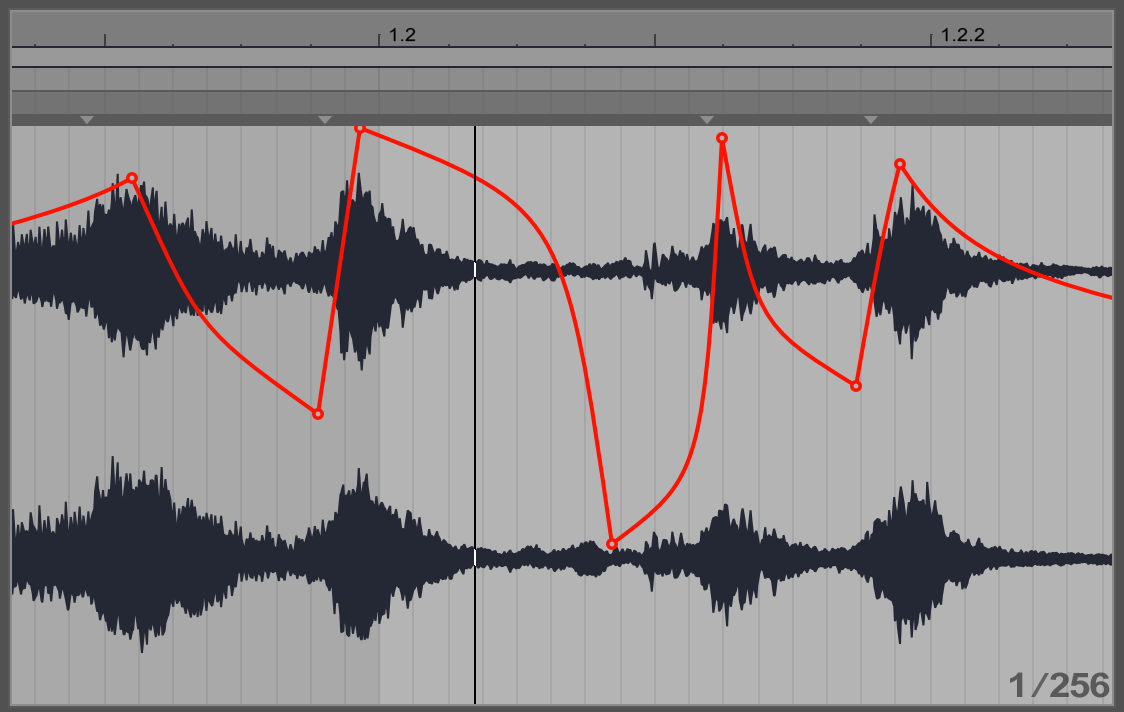
\includegraphics[width=\linewidth]{gfx/03_gesture/AbletonLiveAutomation_72dpi.png}
		\caption{Une courbe d'automation dans le logiciel Ableton Live}
		\label{fig:gesture:automation}
	\end{minipage}
	\hspace{.02\linewidth}
	\begin{minipage}[t]{0.48\textwidth}
	  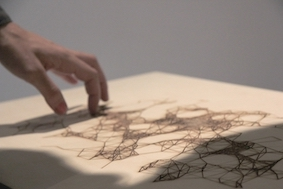
\includegraphics[width=\linewidth]{gfx/03_gesture/EnriqueThomas-TangibleScore_72dpi.jpg}
		\caption{Partition tangible d'Enrique Tomás}
		\label{fig:gesture:tangible_score}
	\end{minipage}
\end{figure}
%------------------ Figure : geste programmé ---------------------
\indent Stiegler développe le concept de ``gramme'' comme \iquote{corps organisé de signes et de symboles} et emprunte à Sylvain Auroux \cite{auroux_revolution_1994} le concept de ``grammatisation'' comme \iquote{le processus par lequel le continuum temporel des comportements humains est transformé en un spatial discret, qui permet de les intégrer dans les outils}. Ainsi en est-il de l'informatique, qui dissocie en symboles et en catégories discrètes ce qui est continu et intégré dans le geste, comme dans le son. Pour Stiegler, les objets sont des enregistrements\footnote{Stiegler utilise les termes de ``rétentions tertiaires'' pour décrire cette inscription de la mémoire dans les objets, afin de la mettre en perspective des ``rétentions primaires'' que sont la conscience du flux temporel et les ``rétentions secondaires'' que sont les souvenirs qui constituent l'expérience d'un individu.}, dans lesquels la mémoire de ce que nous faisons et de ce que nous connaissons est déposée sous la forme d'une mémoire technique.\\
\indent Le concept de Stiegler fait également écho à la notion de ``diagramme'', proposée par Gilles Deleuze dans son étude sur la peinture de Francis Bacon \cite{deleuze_francis_1981} : \iquote{Le diagramme, c'est donc l'ensemble opératoire des lignes et des zones, des traits et des taches asignifiants et non représentatifs. Et l'opération du diagramme, sa fonction, dit Bacon, c'est de suggérer. Ou, plus rigoureusement, c'est d'introduire des «~possibilités de fait~» : langage proche de celui de Wittgenstein. Les traits et les taches doivent d'autant plus rompre aevc la figuration qu'elles sont destinées à nous donner la Figure. C'est pourquoi elles ne suffisent pas elle-mêmes, elles doivent être «~utilisées~» : elles tracent des possibilités de fait, mais ne constituent pas encore un fait (le fait pictural).}\\
\indent On peut voir un parallèle frappant entre cette notion de diagramme et les fonctions assumées à la fois par l'instrument et par la partition musicale. L'instrument de musique contient ainsi l'enregistrement de la théorie musicale qui lui est propre (ses ``traits et ses taches'' que représentent son organisation des hauteurs, sa signature timbrale, son ergonomie, etc.) et que le luthier lui imprime. De même, on peut voir la partition comme un ``enregistrement'' de la pensée et du travail du compositeur, une trace de ses ``gestes sédimentés'' comme le dit Jean-Paul Olive dans \cite{olive_expression_2013}. La composition et la lutherie sont deux formes d’écriture diagrammatiques du geste et du son, qui s’inscrivaient jusqu’alors (avant le numérique) sur des médiums distincts: papier pour la composition, matériaux physiques pour la lutherie. Le numérique offre un médium commun qui permet leur recomposition mutuelle: l'instrument est ``composé'' \cite{schnell_introducing_2002}, la partition est ``instrumentalisée''\footnote{Voir à ce sujet le travail explicite de Enrique Tomás sur les ``partitions tangibles'' \cite{tomas_tangible_2014}} et les gestes de l'expression compositionnelle et de l'expression performative s'interpénètrent \cite{dobrian_e_2006}.\\
\indent Ces gestes programmés ne sont pas de simple enregistrements linéaire à repoduire tels quels, mais des modèles complexes et dynamiques\footnote{Cette idée est développée au chapitre \ref{sec:algorithms:MID}} qui invitent à l'interaction, au jeu\footnote{Cf. les propos de Stiegler dans \cite{stiegler_circuit_2004} \iquote{Quant à la duction de l'instrumentiste, elle vient retemporaliser ce qui ne peut être que spatial : le travail de la composition, ce n'est que spatial, c'est du temps spatialisé, et en cela, essentiellement en défaut d'être. C'est du virtuel pur. C'est du temps discrétisé et détemporalisé dans cette mesure. Discrétisé, il devient manipulable dans sa détemporalisation temporaire telle que la pratique le com­positeur, mais il n'est que virtuel. Il ne peut devenir actuel qu'avec l'interprète, qui doit le re-temporaliser.}}, par le musicien qui n'est pas, justement, un \textit{utilisateur} qui démarre, par exemple, la lecture d'un enregistrement audio. La performance musicale consiste justement à faire entendre ce qui n'est pas calculable comme le dit Stiegler \cite{stiegler_circuit_2004}: \iquote{Un musicien, c'est quelqu'un qui d'abord entend, c'est-à-dire qu'il est primordialement affecté par l'oreille, une oreille qui a cependant des yeux et des mains, et un corps qui les relie. Il ne se contente pas de calculer. Il peut calculer, il doit même calculer, mais s'il le fait, c'est pour donner à entendre ce qu'il a lui-même entendu comme l'incalculable même.}\\
\indent Ce jeu de la main et de l'oreille, qui vient mettre en mouvement ces \textit{gestes programmés} par un geste expressif incalculable, m'amènent à introduire l'idée de geste de ``re-sonnance'', qui se départit du modèle acoustique d'excitation/modulation, en ce qu'il nourrit une relation avec le son qui n'est pas simplement causale mais intègre l'idée d'agencement compositionnel et d'aller-retour entre la temporalité du geste re-sonnant et celle, intrinsèque, du geste programmé.

%-------------------------------------------
\subsection{Le geste de re-sonnance}

\noindent Si les gestes programmés s'apparentent au résultat d'un processus de lutherie/ composition\footnote{Ce processus qui se décline sur différentes échelles temporelles est toutefois réalisables durant le temps même de la performance, en particulier dans le \textit{live-coding}.}, comment donc nommer ces gestes qui permettent de faire sonner un \gls{DMI} ?\\
\indent On ne peut se réduire à les nommer ``gestes d'excitation et de modulation'' (même si la métaphore qui les sous-tend peut s'appuyer sur cette idée), car de nombreux gestes n'évoquent en rien cette dimension physique (e.g. l'ouverture d'un fader de volume).\\
\indent On pourrait utiliser le terme de ``gestes effecteurs'' de Delalande, mais il faudrait les coupler d'une part à un processus dynamique, et d'autre part à une métaphore définissant leur logique. Or dans le cas de l'analyse du jeu pianistique de Gould, le piano est déjà sa propre métaphore, car l'instrument acoustique \textit{est} sa propre interface et son propre modèle intermédiaire à la fois\footnote{Ce qui n'empêche pas d'autres métaphores extra-pianistiques de se superposer à l'instrument et d'en orienter les gestes effecteurs, comme le note Delalande : \iquote{(...) les différents touchers sont pour lui [Gould, NdE] l'équivalent d'une orchestration pour différencier les parties polyphoniques; ainsi le staccato joue-t-il le rôle des \textit{pizzicati} de violon et le grand \textit{legato} de la basse, celui des violoncelles. Il n'est donc pas exclu que certains gestes puissent être dictés par cette imagination orchestrale (...)}}.\\
\indent La notion d'objet sonore-gestuel de Rolf Inge Godøy s'approche le mieux de l'idée présentée ici, en tant qu'elle intègre cette notion de métaphore intermédiaire entre le geste et le son, mais d'une part sa nature ``d'objet'' semble plutôt s'appliquer au modèle intermédiaire lui-même qu'au geste, et d'autre part Godøy semble (malheureusement) en limiter le cadre à une relation de congruence spectromorphologique entre le geste et le son (avec le dessein d'offrir, là-encore, une lisibilité de la relation énergétique).
%---- Figure : Guqin ---------
\begin{figure}[!htbp]
	\captionsetup{format=plain}%
	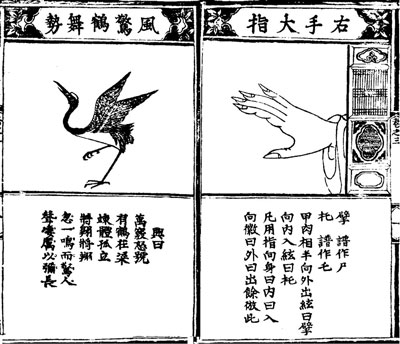
\includegraphics[width=\textwidth]{gfx/03_gesture/Guqin-hand01w.jpg}
	\caption[Le Tayin da quanji : métaphore poétique et animale dans la pédagogie du Guqin]{Un feuillet du \textit{Tayin da quanji} : les gestes instrumentaux du Guqin y sont décrits par un aphorisme poétique, et illustrés par le mouvement d'un animal.}
	\label{fig:gesture:guqin}
\end{figure}
%---- Figure : Guqin ---------
\indent On pourra élargir ce cadre métaphorique au delà de la spectromorphologie en s'inspirant d'un système métaphorique un peu plus ancien et plus ouvert: le ``Tayin da quanji''\footnote{``L’Encyclopédie des sons suprêmes'', ouvrage ayant probablement vu le jour durant la dynastie Song, mais n'ayant survécu qu'à travers diverses éditions, une datant du \siecle{16}~siècle. Une reproduction est disponible en ligne : \url{http://www.silkqin.com/02qnpu/05tydq/ty3.htm}. Voir \cite{picard_chine:_1991}.} décrivant la relation gestuelle-sonore pour l'apprentissage du Guqin dans un ensemble de feuillets comprenant une illustration de la position de main, associée à l'image d'un animal et d'un texte poétique condensant l'esprit du mouvement (cf. figure \ref{fig:gesture:guqin}), par exemple : ``A la manière d'une grue qui danse parce qu'elle est effrayée par une brise.'' Considérons maintenant un hypothétique \gls{DMI} dont le modèle intermédiaire représenterait la gestuelle de la grue durant la dynastie Song; le geste de re-sonnance d'un tel instrument pourrait consister à jouer la brise qui effraie la grue. Ce geste pourrait alors se concrétiser de différentes manières, que cela soit en simulant les mouvements du vent sur une tablette graphique, en agitant les mains munies d'accéléromètres, en soufflant dans un micro, en pinçant des cordes qui --~comme celles du Qin~-- seront sûrement capables d'évoquer le mouvement du vent, si elles parviennent à évoquer la danse de la grue...

\noindent J`utiliserai donc ici le terme de ``gestes de re-sonnance'' pour désigner un geste qui consiste à faire sonner un \gls{DMI} basé sur un ``geste programmé'', c'est-à-dire un modèle dynamique préalablement enregistré, encodé dans le \gls{DMI} et définissant son comportement. Son apparente similitude avec le terme \textit{résonance} n'est pas fortuite : le geste de re-sonnance a affaire à un processus qui possède sa propre dynamique avec lequel il doit s'accorder (ou non) et se mettre ``en résonance''.  

\indent Le ``geste de re-sonnance'' s'appuie donc sur un \textit{modèle intermédiaire} projeté dans l'imaginaire par \textit{une métaphore} : modèle physique appelant des gestes d'excitation, modèle de lecture de vinyle appelant le \textit{scratching}, modèle de robinets-à-son\footnote{Je reprend ici l'expression utilisée par François Dumeaux pour décrire une partie de son interface de jeu. Cf. annexe \ref{appendix:dumeaux}.} controlés par l'ouverture de \textit{faders} sur une table de mixage, modèle cartographique (e.g. interpolation par boules) définissant un terrain à parcourir sur une tablette, modèle de grue effrayée dansant dans la brise, etc. Le geste de re-sonnance se déploie dans un espace polarisé par cette métaphore.\\
\indent Ce modèle est rendu tangible via l'interface, mais l'interface ne définit pas l'ensemble de la métaphore : ainsi un clavier peut servir au déclenchement de notes (comme sur sur un piano), mais si l'intensité des notes est contrôlé par un autre processus (e.g. une pédale d'expression, ou une foule d'agents virtuels autonomes) le clavier ne sera plus envisagé comme une surface ``de percussion'' mais comme un filtre, un crible ne laissant passer que certaines fréquences. Le métaphore du piano avec ses marteaux projetés par l'enfoncement des touches disparait pour laisser place à un autre rapport sensible à l'instrument.\\
\noindent \textbf{contextualité} A la différence du geste d'excitation/modulation/sélection de Cadoz à prétention universelle, le geste de re-sonnance est un geste \textit{contextuel}, dépendant de l'interface, du modèle intermédiaire, de la musique jouée, du contexte de performance. Cette contextualité n'empêche cependant pas qu'une typologie soit établie pour un contexte donné, en s'appuyant sur l'observation des pratiques qui s'y rattachent. C'est par exemple l'objet de la thèse de Baptiste Bacot \footnote{\cite{bacot_geste_2017}}: son analyse qu'il définit comme une \iquote{organologie située}, s'appuie sur l'observation de situations concrètes de performance musicale chez différents instrumentistes numériques, et prend en compte les spécificités de leur configurations instrumentales.\\
\indent C'est aussi le cas dans le travail mené par Nathanaëlle Raboisson et Pierre Couprie, sur l'étude du geste performatif dans l'interprétation de musiques acousmatique sur table de mixage \cite{raboisson_experience_2017}. Une analyse partant de l'observation méthodique des gestes et de leur corrélation (ou non) avec le résultat musical leur permet d'esquisser une typologie propre à cette pratique, incluant des \iquote{gestes de placement} qui participent à la (dé)construction de l'espace sonore, ou encore des \iquote{gestes d'accompagnement}\footnote{Le sens est ici tout autre que le geste d'accompagnement tel que défini par Delalande évoqué précédemment.} caractérisés par une synchronie entre le geste et la morphologie sonore.\\
\indent De même qu'il existe un répertoire gestuel associé aux instruments acoustique, les modèles intermédiaires définissent, de manière modulaire, un vocabulaire d'interaction qui leur est lié. Le geste de re-sonnance s'appuie donc sur les affordances et la structure musicale associées à certains modèles intermédiaires : un geste venant contrôler une boucle de batterie telle que le Amen Break peut s'appuyer sur l'ensemble des techniques de \textit{chopping}\footnote{Dans les musiques basées sur l'utilisation du break-beat, le chopping consiste à découper la boucle de certaines manière en segments plus petits afin de les reconfigurer dans un ordre différent.}, \textit{cutting}, \textit{filtrage} passe-bas, \textit{stuttering}, \textit{varispeed}, etc. qui lui sont historiquement associées.\\
\indent Norbert Schnell développe l'idée de ``ré-animation d'enregistrements audio''\footnote{Le terme anglais \textit{reenactment} utilisé dans son travail reflète mieux que ``ré-animation'' le lien avec la théorie de l'enaction sur laquelle s'appuie notamment son travail.} \cite{schnell_playing_2013} et propose une étude très riche sur le plan théorique comme sur le plan pratique des modalités d'engagement dans une relation gestuelle/sonore par le biais d'une action métaphorique. En particulier, plusieurs exemples s'appuient sur une pièce musicale complète (de Johann Sebastian Bach, en l'occurence) et présentent diverses stratégies possibles d'avancement dans la pièce, sur la base d'une même structure commune définie par l'œuvre de Bach.\\



\subsection{Résonance entre les gestes re-sonnants et programmés}

\noindent Les instruments acoustiques présentent des modes de résonance que l'instrumentiste apprend à connaître, à apprivoiser, pour obtenir les qualités sonores qu'il ou elle recherche. Ces modes de résonance influent sur le timbre qui sera, par exemple sur un instrument à corde, rond et ample si l'on joue la corde au milieu de sa longueur, tandis qu'il sera plus grêle et chuintant si l'on joue \textit{sul ponticello}. La résonance de l'instrument acoustique peut également affecter d'autres paramètres que le timbre, par exemple le rythme : un percussioniste peut mettre à profit le rebond de ses baguettes sur la peau tendue, lors d'un jeu de roulements, et adaptera le poids et/ou la tension qu'il applique sur ses baguettes en fonction de la zone qu'il frappe et de son élasticité.

\indent Cette adaptation dynamique du geste à la résonance de l'instrument prend d'autres dimensions encore dans les \glspl{DMI}, pouvant générer de manière autonome\footnote{L'autonomie totale n'est évidemment plus une situation instrumentale à proprement parler.} toute une phrase musicale, tout un morceau. La nature dynamique et générative des \glspl{DMI} déplace l'agentivité\footnote{La notion d'agentivité dans la performance musicale dépasse sa simple implémentation opérante dans les \gls{IHM}. Par exemple, les figures dialogiques dans la musique classique ont été également analysée à travers ce prisme, voir notamment \cite{graybill_whose_2016}} de l'interaction instrumentale sur un terrain où elle se distribue entre des processus ``qui tournent'' et qu'il s'agit ``d'attraper''\footnote{Guerino Mazzola rapporte cette phrase du mathématicien Jean Cavaillès dans \cite{mazzola_topos_2018}: \iquote{Comprendre, c'est attraper le geste et pouvoir continuer}.} pour en jouer. Un exemple populaire en est l'alignement rythmique entre deux morceaux mixés par un \gls{DJ}, ou lors de l'utilisation d'un \textit{looper}.\\
\indent Le \gls{DMI} peut se retrouver en position de mener le jeu et imposer sa cadence à l'instrumentiste. La performance musicale avec un \gls{DMI} est donc une co-performance où la distribution du contrôle de la synthèse et de la gestuelle qui la provoque, ou en découle, peut se définir de manier polymorphe. Une partie de la dynamique de jeu peut être prise en charge par la machine et une autre partie par l'instrumentiste dans une relation qui peut parfois s'apparenter à un duo\footnote{Cette redistribution dialogique devient explicite dans des dispositifs tels qu'Omax (\cite{assayag_omax_2006}) ou le Continuator (\cite{pachet_continuator:_2003}). Voir par exemple la session d'improvisation entre György Kurtág père et fils avec le Continuator : \url{https://youtu.be/pqfKGlRvddg}.}.


\indent La part d'agentivité respective de la machine et du musicien dans la production du son des \glspl{DMI} définit en fait tout une échelle de nuances, allant de la posture de la personne écoutant la musique ``malgré elle'' (dans un supermarché, typiquement) à celle du musicien engageant tout son corps (physiques, cogécoute) dans l'interaction musicale. Cette recherche de la résonance avec l'instrument, d'en comprendre l'organisation des sons et les rythmes propres, d'en attraper les gestes programmés, d'y trouver les \textit{sweet-spots} est peut-être, davantage que le medium constitutif de l'instrument, ce qui définit vraiment son instrumentalité.

Le développement de l'ésthétique minimaliste n'est pas étrangère à cette capacité de pouvoir saturer l'espace sonore (ou visuel) sans qu'aucun effort ne soit à faire.

La possibilité des \glspl{DMI} de pouvoir générer du son en continu sans qu'aucun effort ne soit nécessaire pose de manière plus radicale que jamais la question de l'engagement du musicien, de quoi jouer et quoi \textit{ne pas} jouer), de quand jouer et quand \textit{ne pas} jouer et de comment le jouer.

La différence des \glspl{DMI} est de définir non-seulement l'agentivité de l'instrumentiste comme définissant les modes de production du sonore, mais également les modes de non-production du sonore, de la part d'instruments capables de produire en continu sans intervention. L'engagement musical avec un processus de génération sonore autonome ne nécessite pas forcément tant de savoir ``quoi'' jouer, mais de savoir en premier lieu ``quand'' jouer (ou ne pas jouer).


Les gestes du musicien peuvent alors entretenir diverses relations:
\vspace{-1em}
\begin{itemize}[noitemsep]
\item une relation d'accompagnement, cohérente (en phase) ou dissonante (opposition de phase);
\item une relation dialogique (typiquement un jeu de question/réponse)
\item une relation de d'alignement;
\item une relation d'accentuation.
\end{itemize}
 
Le geste de résonance qui associe à la fois une fonction ergotique (de type modulation) et une fonction épistémique (en cela qu'on cherche le \textbf{sweet spot}). 


Niveau plus ou moins cohérent de résonance entre le geste et le résultat produit, amène à étudier le résultat perçu dans ces différents cas. (commencer à amener la notion de causalité et de lisibilité présentée dans subversive gestures.)

L'apparence de causalité est fonction de
- congruence temporelle : synchronisation temporelle, morphologie rythmique similaire
- congruence spatiale : colocalisation spatiale, trajectoire similaires
- médiation par un objet intermédiaire dont on pense connaître le fonctionnement


%%%%%%%%%%%%%%%% FIN de cette section ? %%%%%%%%

Les métaphores définissant les relations gestuelles-sonores peuvent être guidées par la recherche d'une certaine lisibilité, comme il a été le cas dans la plupart des travaux pré-cités, qu'elle soit de nature énergétique, spectromorphologique, ou imitative d'instruments existants. Ces relations peuvent toutefois être envisagées dans leur aspect subversif, en profitant de la perception différenciée de l'instrumentiste et de l'auditeur/spectateur.

Un exemple significatif est l'interprétation de ``Hangsimogato N°2'' de György Kurtág Jr\footnote{Vidéo disponible sur \url{https://www.youtube.com/watch?v=MJ8Z5skovLw}}. Dans cette pièce, le développement musical se fait par avancement sur une partition pré-programmé par l'intermédiaire d'un capteur Infra-Rouge (D-Beam). Le capteur lui-même n'est pas sensible à l'orientation de la main ou à quelle main (gauche ou droite) vient couper le rayon, mais György Kurtág Jr développe tout un vocabulaire gestuel qui établit des relations de correspondance avec le son. Ces relations de correspondance peut s'appuyer sur une similarité de morphologie énergétique, mais dans certains cas (e.g. geste de présentation des mains ouvertes vers le ciel, replis des bras en croix) elle sont purement métaphoriques et poétiques.
\todo{rajouter un screenshot de la vidéo de Gyorgy}



Toutes les composantes du son, de la musique, et de la scénographie sont sujettes à l'invention de gestes, selon ce que le musicien décidera comme d'importance pour sa musique.


%%%%%%%%%%%%%%%%%%%%%%%%%%%%%%%%%%%%%%%%%%%%%%%%%%%%%%%%%%%%%%%%%%%

%%%%%%%%%%%%%%%%%%%%%%%%%%%%%%%%%%%%%%%%%%%%%%%%%%%%%%%%%%%%%%%%%%%%
%%%%%%%%%%%%%%%%%%%%%%%%%%%%%%%%%%%%%%%%%%%%%%%%%%%%%%%%%%%%%%%%%%%%


\section{Subversion sonore, subversion gestuelle}
\label{sec:gesture:subversion}
%------------------ Figure : geste lisible ou subversif ---------------------
\begin{figure}[!htbp]
	\captionsetup{format=plain}%
	\centering
	\begin{minipage}[t]{0.48\textwidth}
		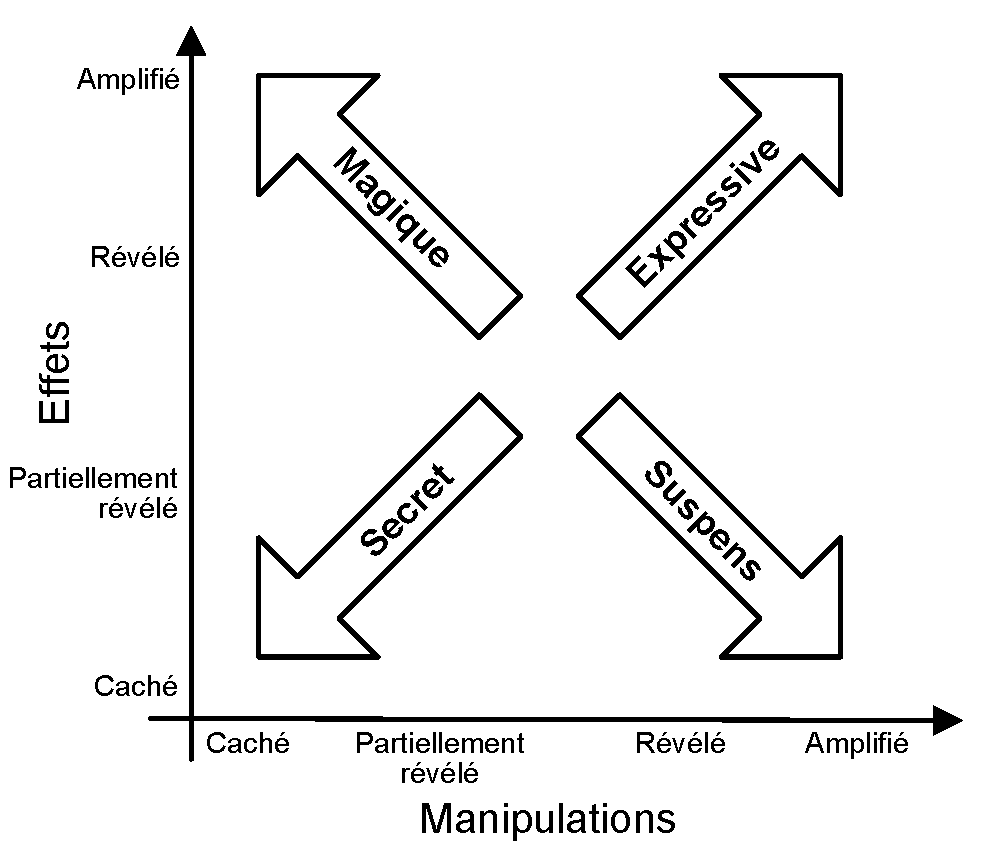
\includegraphics[width=\linewidth]{gfx/03_gesture/ManipulationVsEffect2.pdf}
		\caption{Visibilité de la manipulation et de l'effects (``Strategies for designing spectator interfaces.'') dans \cite{reeves_designing_2005, benford_performing_2010}}
		\label{fig:gesture:Benford}
	\end{minipage}
	\hspace{.02\linewidth}
	\begin{minipage}[t]{0.48\textwidth}
	  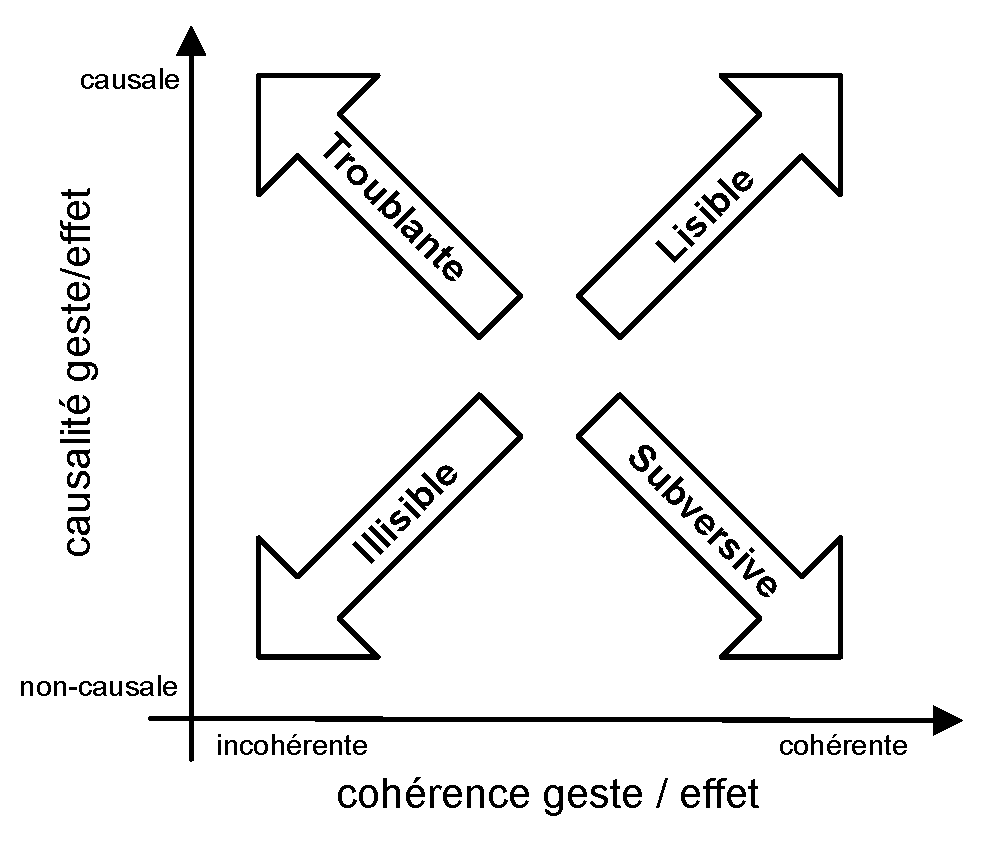
\includegraphics[width=\linewidth]{gfx/03_gesture/CoherenceVsCausalite2.pdf}
		\caption{Lisibilité et subversivité de la relation geste/effet}
		\label{fig:gesture:lisibility_subversion}
	\end{minipage}
\end{figure}

Comme nous l'avons dit précédemment, la relation de causalité entre le geste et le son dans les \glspl{DMI} n'est pas une donnée

Perception d'erreur du point de vue du spectateur \cite{fyans_ecological_2012}

\cite{emerson_gesture-sound_2018}

Reeves et Benford propose un modèle de stratégies pour le design ``d'interfaces spectateurs'' montrant les effets obtenus lorsque la manipulation (les gestes de l'instrumentiste dans le cas qui nous intéresse ici) et l'effet de cette manipulation (le son dans notre cas) présentent chacun des degrés divers de visibilité.

Dans la figure de Benford manque la possibilité que la visibilité ne soit pas causale de l'effet.
Ce qui nous manque ici est la possibilité que la partie visible de la manipulation ne sont pas la cause de l'effet.

La cohérence\footnote{J'appelle ici ``cohérence'' la causalité \textbf{apparente} entre le geste et le son, pour la distinguer de la causalité \textbf{effective}, avec laquelle elle est mise en regard. La littérature en psychologie cognitive utilise cependant davantage le terme de perception de causalité.} entre le geste et le son se base sur un ensemble de valeurs qui ont été analysée dans de nombreux articles de sciences cognitive\footnote{Voir par exemple \cite{michotte_perception_2017}, ouvrage récent qui compile un grand nombre d'effets amenant à une perception cogérente}, en particulier celles de la théorie de la perception, telles que :
\vspace{-1em}
\begin{itemize}[noitemsep]
	\item la congruence temporelle : syncrhonisme, destin commun, si j'entend le son en même temps que le geste, alors c'est ce geste qui a produit ce son.
	\item la congruence spatiale : si j'entend le son venir d'un endroit précis et que l'instrument se trouve à ce même endroit, alors le son vient de l'instrument.
- médiation par un objet intermédiaire dont on pense connaître le fonctionnement
\end{itemize}


\vspace{-1em}
\begin{itemize}[noitemsep]
	\item \textbf{lisible} : la perception du geste et du son apparait cohérente par rapport au système. Par exemple : on voit et on entend une personne parler.
	\item \textbf{illisible} : on voit une personne parler et on entend une autre voix
	\item \textbf{troublante} : c'est le cas du ventriloque : il est bien responsable du son que l'on entend (causalité), mais l'absence de mouvements de lèvre rend la perception visuelle incohérente avec la parception sonore (dissonance cognitive entre vue et ouïe).
	\item \textbf{subversive} : c'est le cas du playback
\end{itemize}

\subsection{Définition} 

Le terme ``subversion'' (du latin \textit{subvertere} : renverser, bouleverser) désigne ``l'action visant à saper les valeurs et les institutions établies'' (dictionnaire Larousse). Les moyens employés par la subversion consiste à diffuser un message contraire à un l'ordre établi, dans le but d'affaiblir celui-ci.

Dans le cas de la musique, si la notion de subversion peut prendre une dimension culturelle ou politique dans certains courants musicaux, c'est ici dans le cadre de la perception que j'emploie ce terme.

La subversion peut intervenir à différents niveaux. Au niveau de la composition, l'écriture musicale permet des modulations qui déjouent les attentes de l'auditeur. (e.g. Pink Floyd, breathe transition). Elle peut également se situer au niveau du jeu, en usant de procédés comme des gestes qui contredisent ce qu'on entend et vont l'amplifier. Gyorgy Kurtag Jr. geste violent pour jouer une nuance pianissimo.

Exemples comparés de Applebaum Aphasia et Vincent Carinola/Jean Geoffroy "Virtual Rhizome".
BBC Classic Album: "Pink Floyd - The Dark Side of the Moon"

Dissonance cognitive.

Synchrèse de Michel Chion.

Parler du playback, du air-guitar, de la synchrèse.

Nattiez, Music and discourse p44 : certain pianistes ont l'impression de donner de la ``profondeur'' à un accord en permettant aux doigts de glisser vers l'intérieur du piano après avoir enfoncé les touches. (...) inversement, Braendel : le son de notes soutenues sur le piano peut être modifié... à l'aide de certains mouvements qui rendent la \textit{conception du cantabile} du pianiste visible pour le public. (Delalande, ``vers une psycho-musicologie'' in L'enfant du sonore au musical):166, (Brendel, A. 1976. Musical Thoughts and Afterthoughts. Princeton: Princeton University Press. p.31)

Bien que ces catégorisations du gestes décrivent adéquatement différents aspects du geste instrumental sur des instruments acoustiques, il semble que le geste musical intègre une aspect subversif souvent négligé.

En particulier, dans le cas des \glspl{DMI}, la relation entre le geste et le son est totalement sujette au design de ce que l'on nomme communément le \gls{mapping} et la part de subversion devient partie intégrante du design de ce mapping. 


Il semble dès lors que l'on peut envisager d'autres types de relation entre le geste et le son, afin de tenter de décrire les différents rapports qu'ils entretiennent selon les situations.

Risset fait remarquer l'importance de l'histoire du son d'origine mécanique dans la perception des sons \cite{risset_son_1992}: 

\begin{quotation}
II semble à première vue que l'acoustique numérique puisse s'affranchir de la mécanique. Cependant notre ouïe a évolué dans un environnements d'objets vibrants: aussi la prise en considération des contraintes et des particularités des vibrations mécaniques est-elle importante pour comprendre les idiosyncrasies de la perception auditive et pour en tirer parti.

Les limites de l'acoustique numérique dépendent des capacités différentielles de perception davantage que des contraintes mécaniques. Pourtant, notre perception auditive est orientée par un monde de sons produits mécaniquement, et la mécanique ne doit pas être écartée de façon cavalière, comme l'ont suggéré les travaux de Gibson et Cadoz : les spécificités des vibrations mécaniques mettent en lumière l'organisation perceptuelle dans le processus auditif


\footnote{The limitations of digital acoustics depend upon the differential capacities of perception rather than upon the constraints of mechanics. Yet our auditory perception is geared to a world of mechanically-produced sounds, and mechanics should not be given a cavalier dismissal, as the work of Gibson and Cadoz has suggested : the specifics of mechanical vibrations shed light on the the perceptual organization in the hearing process.} TODO : traduire l'anglais, plus riche.
\end{quotation}


\textbf{Proposition}
\vspace{-1em}
\begin{itemize}[noitemsep]
\item readable gesture to sound relations
\item confusing gesture to sound relations
\end{itemize}

\vspace{-1em}
\begin{itemize}[noitemsep]
\item Gestes emphatique = en phase avec le mouvement interne du son
\item Geste apophatiques = en opposition de phase avec le son
\item Geste unrelated
\end{itemize}

%---- Figure : Einarsson sculpture ---------
\begin{figure}[!htbp]
	\captionsetup{format=plain}%
	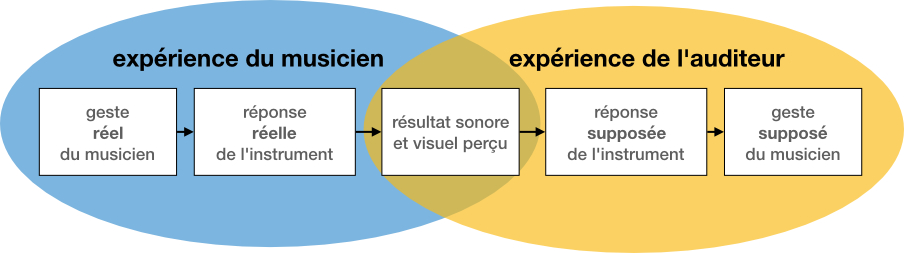
\includegraphics[width=\textwidth]{gfx/03_gesture/gesteReelGesteSuppose.jpg}
	\caption{Geste produit, geste perçu, fonctionnement réel et supposé de l'instrument}
	\label{fig:gesture:RealVsSupposed}
\end{figure}


%-------------------------------------------
\subsection{Sons paradoxaux, gestes paradoxaux}
Risset, Kurtag Jr., Kurtag Père

De la même manière que l'écriture musicale sur papier a permis de développer des processus de compositions difficilement pensables sans ce support visuel \footnote{tels que la rétrogradation ou la fugue}, les ordinateurs ont permi de créer des formes sonores qu'il aurait été impossible de concevoir sans cet outil computationnel, tels que les sons paradoxaux de Risset et Shepard \footnote{qu'il n'est toutefois pas impossible de reproduire sans recourir à l'ordinateur, telle démontrée que cette interprétation des glissandi de Risset à la voix par Victoria Hart \url{https://vimeo.com/147403169}}

aspect scénographique de la performance musicale.
\vspace{-1em}
\begin{itemize}[noitemsep]
\item \textbf{gestes de feintes} : déception de l'attente, mais visible après coup. E.g. dans le football, faire semblant d'aller à droite et envoyer le ballon à gauche, en musique: ommettre le temps fort d'un rythme bien établi, etc. La mécanique du geste est entièrement visible mais a été confuse par un changement innatendu.
\item \textbf{geste magique} : La mécanique du geste reste invisible et la logique causale entre le geste et son résultat reste inexplicable, et sujette à spéculation imaginaires.
\end{itemize}


%---- Figure : Triggering modes ---------
\begin{figure}[!htbp]
	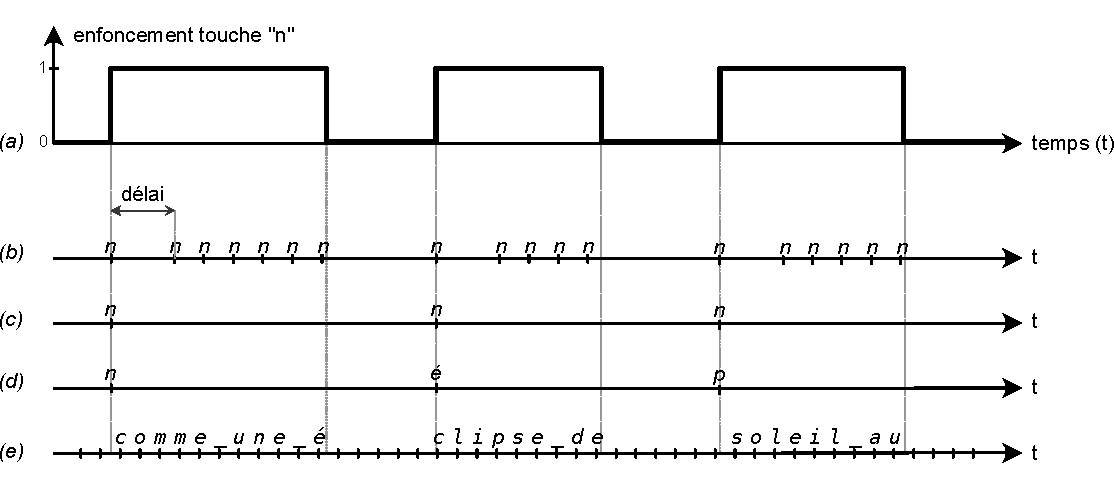
\includegraphics[width=\textwidth]{gfx/03_gesture/key_modes.pdf}
	\caption{Différents modes de déclenchement: (a) enfoncement de la touche ``n''; (b) comportement habituel d'un clavier (e.g. dans un traitement de texte) (c) suppression de la répétition (d) utilisation d'un réservoir (e) phrases séquencées rythmiquement}
	\label{fig:gesture:triggering_modes}
\end{figure}


%-------------------------------------------
\subsection{Continuités artificielles}

\vspace{-1em}
\begin{itemize}[noitemsep]
\item Contrepoint : relier la mélodie à l'harmonie 
\item Bach et le tempérament = relier les différents modes, via la modulation.
\item les doigtés alternatifs, sur le plan gestuel, permettent de sacrifier la justesse de la note, pour établir une continuité gestuelle fluide
\item La musique sérielle : relier la gamme tempérée au spectre en ordonnant 
\item Stravinsky, Russolo : relier l’harmonie et le bruit 
\item jouer un pattern connu ("qu'on a dans les doigts") tout en substituant les notes permet de jouer de manière fluide une mélodie inhabituelle. => numérique
\item Cage, Murray Schaeffer : relier le déterminisme et le hasard, la musique et l’environnement 
\end{itemize}

(morpho-dynamisme)
Mettre capture d'image du MID qui passe d'une structure rotative à un Verlet.

Comment la continuité s'établit ?

=> voir Théories de la composition musicale au \siecle{20}~siècle
Conjointement à ces explorations compositionnelles se sont développées des techniques et des technologies permettant d’appréhender ces nouveaux espaces. Que cela soit des procédés d’écriture ou des instruments reflétant ces méthodes et modèles.


%%%%%%%%%%%%%%%%%%%%%%%%%%%%%%%%%%%%%%%%%

 
\section{Conclusion}
\label{sec:gesture:conclusion}


\noindent On voit donc que la relation entre le geste et l'instrument a été considérablement affectée par l'introduction de l'électricité, mais plus encore du numérique, dans le corps de l'instrument. Ces relations se construisent sur un medium présentant des caractéristiques radicalement opposées à celles de l'instrument acoustique : l'absence de causalité et de continuum énergétique entre le geste et le son, le métamorphisme du comportement de l'instrument, et l'absence possible de contact physique entre le geste et l'instrument.

Dans ce contexte, plusieurs voies sont possibles. 
La recherche d'une lisibilité de la relation geste/son peut s'appuyer sur des modèles physiques recréant artificiellement les conditions perdues de l'instrument acoustique, ou encore sur des relations basées sur la relation spectro-morphologiques entre mouvements du geste et mouvements du son.

Ces gestes peuvent également s'appuyer sur une connaissance du déroulement interne d'un matériaux enregistré, auquel cas une relation de re-sonnance / résonance vient définir une modalité de relation instrumentale ou les mouvements gestuels ne sont pas nécessairement dans une relation mimétique, mais viennent s'articuler sur différents plans de jeu mêlant écoute, extrapolation imaginaire, [ré]agencements à la volée et anticipatifs, gestes muets dont l'action n'est perçue que de manière différée, etc.



De même que l'on peut travailler une partition et devenir expert dans son interprétation, on peut travailler un instrument pour en devenir expert et travailler les différentes compositions pour cet instrument. On peut aujourd'hui travailler le geste (et l'écoute!) et en devenir expert pour jouer les différents instruments qui s'offrent à ces gestes.


Tout relation semble possible, si tant est qu'il


La relation se définit de manière contextuelle. 

Il est important de comprendre qu'il n'y a plus de relation fixe entre le geste



=> Comment ces aspects influencent le design de l’instrument ?
De cette étude du geste instrumental, on peut retenir plusieurs éléments qui viennent orienter (todo, better word) le développement des briques de bases qui constituent les DMIs.

\vspace{-1em}
\begin{itemize}[noitemsep]
\item transgression des catégories (entre continu et discret, entre audio et non-audio, création de relation arbitraires entre paramètres orthogonaux)
\item absence de limites arbitraires dans les représentations numériques (e.g. ambitus de pitch, polyphonie maximale)
\end{itemize}

\vspace{-1em}
\begin{itemize}[noitemsep]
\item \textbf{le format de données} : doit permettre le polymorphisme (cf. Zicarelli ``numbers without meaning'') entre les diverses formes de captation du geste (signal, événement, présence stable ou éphémère, etc.)
\item \textbf{le mapping} entre variables est lui-même sujet à une reprogrammation dynamique durant le jeu
\item \textbf{les différents gestes} de composition, de performance, d'écoute font partie intégrante des gestes de lutherie
\end{itemize}







\section*{extra material}
Notion de vivadi

Part of the excitment in the domain of new digital musical instruments in the 21st century can be attributed to the fact this fact as the musical creativity goes beyond the sound itself and includes the system through which it is performed. A downside of this situation, however, is that the novelty and digital features if the instruments create a sense of discontinuity with tradition , alienation, and lack of understanding by the audience as to what the instrument or the performer is actually doing.
\cite{magnusson_sonic_2019}



\iquote{Si ça se trouve, cette notion que dans quelques années, ``tout sera possible avec la technologie'' fera que cela sera compliqué de créer un mystère entier et profond, parce que les gens du coup diront ``oui, j'en ai entendu parler, maintenant on peut faire ça''.
 J'ai un ami (...) qui a fait voler un espèce de morceau de tulle au dessus des gens avec des principes mécaniques, et beaucoup de gens disaient ``ah oui, c'était incroyable mais je pense que c'était un drône'', alors que pas du tout. Mais je me suis dit, c'est vrai que d'ici quelques années, un objet qui vole tout seul en silence dans l'espace, n'aura plus le même pouvoir de mystère qu'il y a quelques années.} Yann Frish dans \url{https://www.youtube.com/watch?v=5BqHXbQC36M}





Subversion du geste : Kagel et le théâtre musical.
\url{https://geste.hypotheses.org/gemme}

\iquote{Dans le domaine du geste, les outils technologiques peuvent bien sûr jouer un rôle complice, démultipliant les perspectives, inversant les conséquences attendues, décelant l'infime ou captant par méthode statistique tel ou tel paramètre du jeu musical.} 
\iquote{(...) s’approprier à la manière d’un mime les gestualités sonores qui, malgré les indications de la partition, ne peuvent être réellement considérées et donc interprétées que via le prisme de l’écoute.}
P. Jodlowsky \cite{jodlowski_geste_2006}



\noindent Jakboson (1960) :
\vspace{-1em}
\begin{itemize}[noitemsep]
\item \textbf{expressive function}
\item \textbf{representational functionparce que les attributs qu'on lui confère dépendent en partie de cette qualité sémiotique, qui reste soumise à une interprétation subjective et contextuelle dans un système de valeurs.}
\item \textbf{conative function}
\item \textbf{phatic function}
\item \textbf{metalingual function}
\item \textbf{poetic function}
\end{itemize}

\noindent David McNeil : 
\vspace{-1em}
\begin{itemize}[noitemsep]
\item \textbf{Iconics} where the gesture resembles the referent (e.g. describing an action or shape of an object with the hands).
\item \textbf{Metaphorics} where the vehicle (the gesture) relates in one of a number of metaphorical ways to the tenor (non-literal meaning) of the gesture, e.g. indicating a container or conduit for ideas, or a gift of an idea or suggestion (cf. Lakoff et Johnson 1980).
\item \textbf{Beats} where the hand, head, eybrows move roughly in synchrony with the rhythm of often emphatic speech, mark a sequence, or a hiatus such as a change of theme or focus.
\item \textbf{Cohesives} which create a gestalt in gesture space which is coextensive with a spoken utterance or – hierarchically – with its parts.
\item \textbf{Deictics} which may indicate an actual physical position, size, distance or direction, but may also place concepts metaphorically in physical gesture space
\end{itemize}


La mémoire et les gestes:
Leroi Gourhan

\iquote{Quant à l’action relayée (force motrice et transmission), elle domestique pour les utiliser des éléments qui étendent et complètent les effets techniques. Dans ce stade évolué, on n’est plus dans le faire mais dans le faire faire, engagé dans la voie techno-scientifique qui ne garde du geste humain initial que ses épures et en analyse indéfiniment les schèmes.} Michel Guérin, \cite{guerin_philosophie_2018}


\iquote{Les propos des instruments qui nous entourent ne sont pas obligatoirement les nôtres. Ils appartiennent à ceux qui ont fait produire les instruments. Les détourner, c’est se libérer. Les instruments récents sont fascinants parce que, plus que tout autre, ils abritent des virtualités ignorées et parce qu’ils permettent des actions libératrices.} Michel Guérin, \cite{guerin_philosophie_2018}









Partant de l'idée que le geste et la musique sont deux phénomène impliquant le mouvement, je chercherai donc à définir l'intention gestuelle en fonction du rapport qu'il entretient avec le mouvement musical.
On peut dès lors envisager trois attitudes principales :
\vspace{-1em}
\begin{itemize}[noitemsep]
\item \textbf{jouer avec} : en phase avec le mouvement de la musique (geste emphatique), en soutenant par un rythme ou une harmonie complémentaire à ce qui est joué
\item \textbf{jouer contre} : jouer contre le mouvement pour chercher à l'annuler ou le détruire (geste apophatique)
\item \textbf{jouer indifféremment} : sans chercher à être ni contre, ni avec
\end{itemize}

On pourra nuancer cette catégorisation brutale en ajoutant une quatrième catégorie, qui se situerait entre 
le jeu ``avec'' et le jeu ``contre'' qui consiste à jouer en ``interférence'', c'est-à-dire qui vient infléchir une direction


\iquote{J'appelle technique un acte traditionnel efficace (et vous voyez qu'en ceci il n'est pas différent de l'acte magique, religieux, symbolique). Il faut qu'il soit traditionnel et efficace. Il n'y a pas de technique et pas de transmission, s'il n'y a pas de tradition.} Marcel Mausse, les techniques du corps

Il manque un élément important dans cette considération de la tradition. Pour qu'une tradition soit transmise, il faut que des individus la transmette. Cela peut se faire par la contrainte ou un système doctrinal (e.g. un système religieux), mais en cette absence de coercition physique ou mentale, la tradition sera transmise à la condition que les individus croient en la valeur de cette tradition et qu'ils lui accordent suffisament d'importance pour en mémoriser les principes.


%-------------------------- Figure : Shannon ----------------------------------
\begin{figure}[!htbp]
	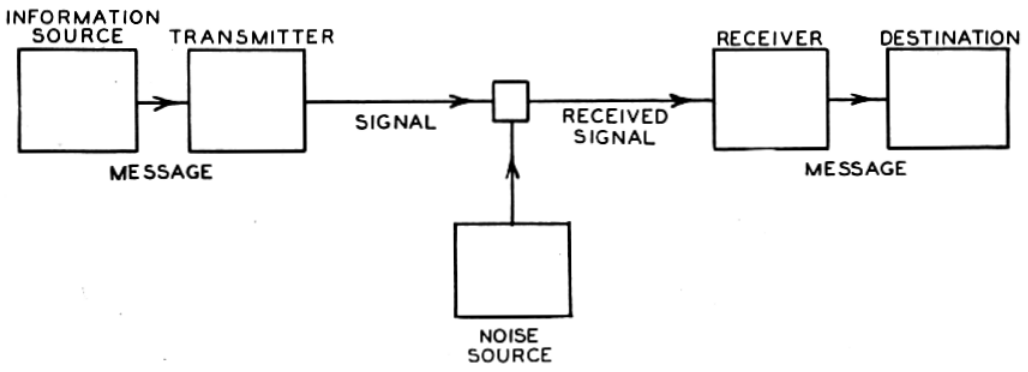
\includegraphics[width=\textwidth]{gfx/03_gesture/ShannonCommunicationSystem.png}
	\caption{Diagramme schématique d'un système général de communication, tel que proposé par Shannon.}
	\label{fig:gesture:shannon}
\end{figure}



Ces deux catégories de geste d'action et de gestes perçu sont emprunt de la théorie de l'information proposée par Shannon \cite{shannon_mathematical_1948} qui envisage la communication comme un système émetteur-message-récepteur unidirectionnel. 
L'inconvenient d'envisager le geste comme simple émetteur d'un signal (qu'il soit travail ou signe) est qu'il empêche de considérer le geste dans la rétroaction dans laquelle il s'inscrit avec l'instrument. En particulier dans la performance musicale, la rétroaction multimodale (par l'ouïe, la vue, le toucher) entre les geste d'un instrumentiste et son instrument, le son et le public est essentielle.

Il était tentant de l'appliquer à la situation musicale et de voir dans le phénomène sonore un message circulant du musicien vers l'auditeur, et les analyses du geste instrumental s'appuyant sur cette solide base théorique ont permis de développer un certain nombre de concept encore utile pour l'analyse du geste musical.

Cependant, la situation de performance musicale est loin d'être aussi fonctionnelle que celle qui consiste à vouloir transmettre un flux de données. Notamment, la théorie de l'information s'applique à des machines qui ignore totalement le contenu sémantique de ces données et les aspects cognitifs ou les références culturelles des émetteurs et récepteurs.
%-------------------------- Figure : transparence Fels -----------------------
\begin{wrapfigure}[14]{R}{0.5\textwidth}
	\begin{center}
 		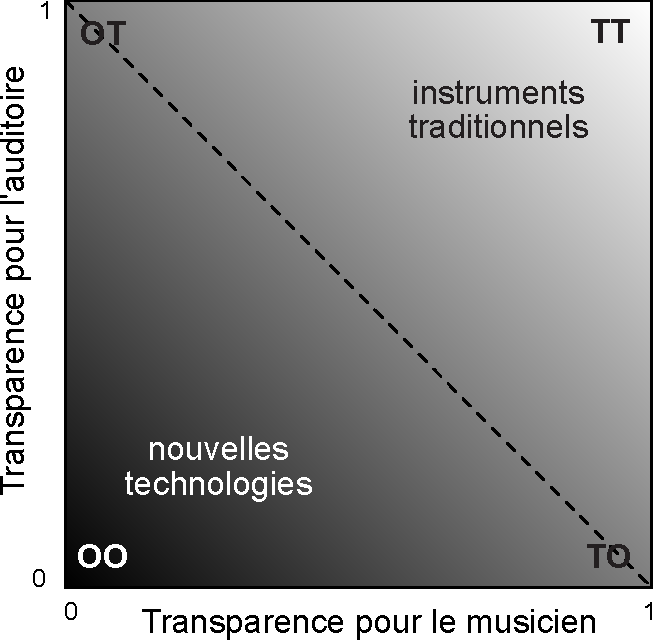
\includegraphics[width=0.48\textwidth]{gfx/03_gesture/Fels-transparency.pdf}
	\end{center}
	\caption{Transparence pour le musicien et l'auditoire, d'après \cite{fels_mapping_2002}}
	\label{fig:gesture:fels_transparency}
\end{wrapfigure}
%-------------------------- Figure : transparence Fels -----------------------

Certains auteurs ont critiqué cette approche \cite{fyans_where_2009} en remarquant que l'idée selon laquelle une connaissance et une compréhension préalable de l'instrument et de l'idiome était nécessaire pour évaluer une performance musicale, ne pouvait être généralisée aux \glspl{DMI}, à cause de l'émergence rapide de technologies, d'instruments et de pratiques de performance dans ce domaine. 

Cependant, cette critique reste ancrée sur une approche qui considère que le spectateur évalue le \textit{succès} d'une performance selon sa compréhension des intentions de l'instrumentiste.


Le jeu musical joue en partie sur l’attente de l’audience (récompensée ou non) sur la base de règles d'harmonies, d’idiomes (e.g. cadences, résolutions, cycles rythmiques), de citations (e.g. via le sampling), etc..
Affordance des instruments ne peut être réduite aux objectifs d’affordance des IHM.


Kurtag Jr. Hangsimotato (video)
Jean Haury Meta-Piano
Applebaum Aphasia

gestes incongruent (Musical gestures, Godoy, p.48)


Charlotte Moorman and Name June Paik performing John Cage’s 26’1.1499” for a String Player (Human Cello section

%%%%%%%%%%%%%%%%%%%%%%%%%%%%


Si le geste est un mouvement accompagné d'intention, il faut prendre en compte cette partie intentionelle et essayer de la qualifier, dans la perspective des conséquences qu'elle porte au design des \glspl{DMI}.

La notion ``d'image de son (i-son)'' de François Bayle exprime la mécanique psycho-poétique de construction de l'œuvre musicale acousmatique. Sa nomenclature ne se prête pas facilement à une application directe dans la lutherie (numérique ou non).
En partant de la classification des fonctions de l'écoute proposée par Pierre Schaeffer et Michel Chion (\cite{chion_guide_1994}, p.26) (Insérer ici le tableau comprendre-écouter-entendre-ouïr), François Bayle retient notamment trois niveaux d'écoute attentive (en regroupant entendre et comprendre dans un seul niveau) qu'il fait correspondre à trois niveau d'intentionalité dans la mise en jeu des \textit{images-de-sons}:
\vspace{-1em}
\begin{itemize}[noitemsep]
\item \textbf{\textit{im-son}}: l'image isomorphe, iconique, référentielle;
\item \textbf{\textit{di-son}}: le diagramme, sélection de contours simplifiés, indiciels ;
\item \textbf{\textit{mé-son}}: la métaphore ou métaforme, reliée à une généralité
\end{itemize}

Ces trois catégories font également écho au catégories de Delalande (gestes effecteurs, gestes accompagnateurs, gestes figurés) — sans qu'il y ait toutefois de relations causales triviales entre ces catégories du gestes et de l'écoute.

%------------------ Bricout: g-son -------------------------
Concept de \textit{g-son} proposé par Bricout \cite{bricout_les_2011}, à partir du concept d'i-son (\textit{image-son}) proposé par Bayle, comme ``dépassement de la suggestion de l'image par le son lui ajoutant de manière beaucoup plus évidente la suggestion du geste, de l'élan physique.''

Romain Bricout : couple ``déclenchement/modulation'' (analogue à l'archétype ``percussion/voix'' Martin Laliberté) comme atomes gestuels constitutif de tout mouvement. => NON tout l'espace gestuel avec toutes les connotations possibles (sémiotiques, mimétiques)

Bricout :
\iquote{Déclenchement et modulation représentent donc ces deux gestes primordiaux, à la base de de n'importe quel autre geste plus complexe. Par voie de conséquence, n'importe quel son renvoie lui-même à un geste producteur qui se rapprochera tantôt du déclenchement, tantôt de la modulation ou, par combinaison, des deux à la fois}
=> qu'en est il d'un field recording ?
%------------------ END Bricout: g-son -------------------------

J'aurais plutôt tendance à employer le terme ``d'image de geste'' (i-geste) pour décrire cette analogie entre les plans d'interprétation du geste et du son.

Le travail de création des correspondances entre geste et son passe ainsi par trois étapes faisant écho à ces différents niveaux de perception/compréhension musicale :
\vspace{-1em}
\begin{itemize}[noitemsep]
\item \textbf{coder} la relation algorithmique (causale ou non), c'est-à-dire concrètement la relation algorthmique qui s'opère entre les signaux captés par l'interface et le contrôle de la synthèse sonore, 
\item\textbf{jouer} la relation sensible, c'est-à-dire pratiquer (chorégraphier) l'ensemble du mouvement gestuel dont une partie seulement sera captée par l'interface de jeu;
\item\textbf{imaginer} la relation poétique, cette relation s'établit sur un ensemble plus complexe de valeurs esthétiques, de références culturelles impliquant de manière plus globale les questions de composition, de scénographie, de métaphores portée par les sons, etc.
\end{itemize}




\subsubsection{Les unités sémiotiques temporelles}

La définition des UST est donnée dans \cite{timsit-berthier_les_2004}:
\iquote{Les UST sont des segments musicaux, qui possèdent une signification temporelle en raison de leur organisation morphologique et cinétique. Elles peuvent êtres considérés comme des représentations iconiques qui entretiennent des rapports de ressemblance avec des modèles temporels naturels. L’UST ne traduit pas le phénomène musical à son niveau acoustique, mais cherche à y trouver en quelque sorte une intentionnalité.}



%%%%%%%%%%%%%%%%%%%%%%%%%%%%%%%%%%%%%%%%%%%%%%%%%%%%%%%%%%%%
%%%%%%%%%%%%%%%%%%%%%%%%%%%%%%%%%%%%%%%%%%%%%%%%%%%%%%%%%%%%
%%%%%%%%%%%%%%%%%%%%%%%%%%%%%%%%%%%%%%%%%%%%%%%%%%%%%%%%%%%%
%%%%%%%%%%%%%%%%%%%%%%%%%%%%%%%%%%%%%%%%%%%%%%%%%%%%%%%%%%%%
%%%%%%%%%%%%%%%%%%%%%%%%%%%%%%%%%%%%%%%%%%%%%%%%%%%%%%%%%%%%
%%%%%%%%%%%%%%%%%%%%%%%%%%%%%%%%%%%%%%%%%%%%%%%%%%%%%%%%%%%%
%%%%%%%%%%%%%%%%%%%%%%%%%%%%%%%%%%
\section*{Espace du geste musical}
La musique a longtemps été considéré comme étant faite d'un sous-ensemble de sons, les sons harmonieux, voire harmonique, avant qu'au \siecle{20}~siècle, les bruits n'y fassent leur place avec les avant-gardes, futuristes. 

John Cage in \cite{cage_silence:_1961}
\begin{quotation}
\noindent If this word, music, is sacred and reserved for eighteenth- and nineteenth-century instruments, we can substitute a more meaningful term: organization of sound.\\
\end{quotation}


Anecdote De Laubier ` le haut parleur ne fonctionne pas'

La musique n'est donc pas faite que de sons, au sens acoustique du terme, mais également (avant tout?) de la perception des sons, qui implique des processus de cognition, des références socio-culturelles, et une sensibilité, une mémoire propre à chacun. 
Ainsi, l'espace de la musique ne se présente non pas comme un sous-ensemble de l'espace des sons, mais probablement comme un sur-espace comprenant à la fois les sons acoustiques mais également tous les liens qu'ils tissent avec notre mémoire.

\Pierre{ voir les 2 définitions de la musique}

L'art musical consiste ainsi à faire entendre des aspects de la musique qui ne sont pas nécessairement présents dans le son, à faire surgir des espaces qui ne peuvent se déployer que dans notre imaginaire, en faisant écho à la trace latente que les sons et la musique ont déjà imprimée en nous.


\begin{quotation}
\noindent Le musical dépasse le sonore en cela qu’il est connecté à une expérience cognitive qui implique la perception et la mémoire.\\
Le sonore dépasse le musical en cela que tout ce qui est sonore ne fait pas nécessairement musique (sauf chez Cage).
\end{quotation}

\Pierre{ ce n'est pas seulement le cas de la musique mais aussi de la parole. Voir définition de Castellengo.}
\Pierre{ Cage -> référence ?}

Là où la présence du musicien sur scène remplissait une nécessité acoustique pour l’écoute, la musique sur support, ou produite par des machines, déplace ce besoin au profit d’une autre fonction, à la fois de compréhension des gestes du musicien (mais est-ce là un jeu de dupes?) et d’un spectacle de l’ordre du funambulisme; le musicien prend des risques [celui de se tromper dans le cas de l’interprétation d’une partition] et la mise en question du corps, réagir au contexte (lieu et au public, ainsi qu’aux éventuels autre musiciens) d’une manière vivante.

L’écoute nous plonge dans des flux sonores, et notre tendance à projeter des causes à ces sons (cf. gestalt) nous emmène sur les lieux — toujours en partie étrangers — de la production de ces flux. sitar indien, crissement de pneu, explosion, acoustique sous-marine ou ambiance de salle de café.
Le musicien crée des passerelles et des agencements entre ces zones liminales.

\Pierre{ si tu parles de gestalt, il faut développer mais c'est aussi une théorie très controversée, donc attention !}

Si les gestes \textit{subversifs} peuvent être assimilés à des gestes accompagnateurs, la plupart des articles de la littérature semble ignorer cette part de subversion au profit de la lisibilité du geste et sa corrélation avec le son \cite{godoy_exploring_2006}.
Cependant, la corrélation n'est pas nécessairement recherchée en tant que telle et si, comme le rappelle Risset, \iquote{la musique est aussi un art du mirage, de l’illusion} \cite{risset_propos_2010}, les œuvres sont nombreuses qui cherchent à dépasser le lien d'apparente causalité entre le geste et le son. 
Il serait alors plus juste d'utiliser le terme de \textit{geste accompagnant la musique}, si toutefois on 

%---- Figure : Einarsson sculpture ---------
\begin{figure}[!htbp]
	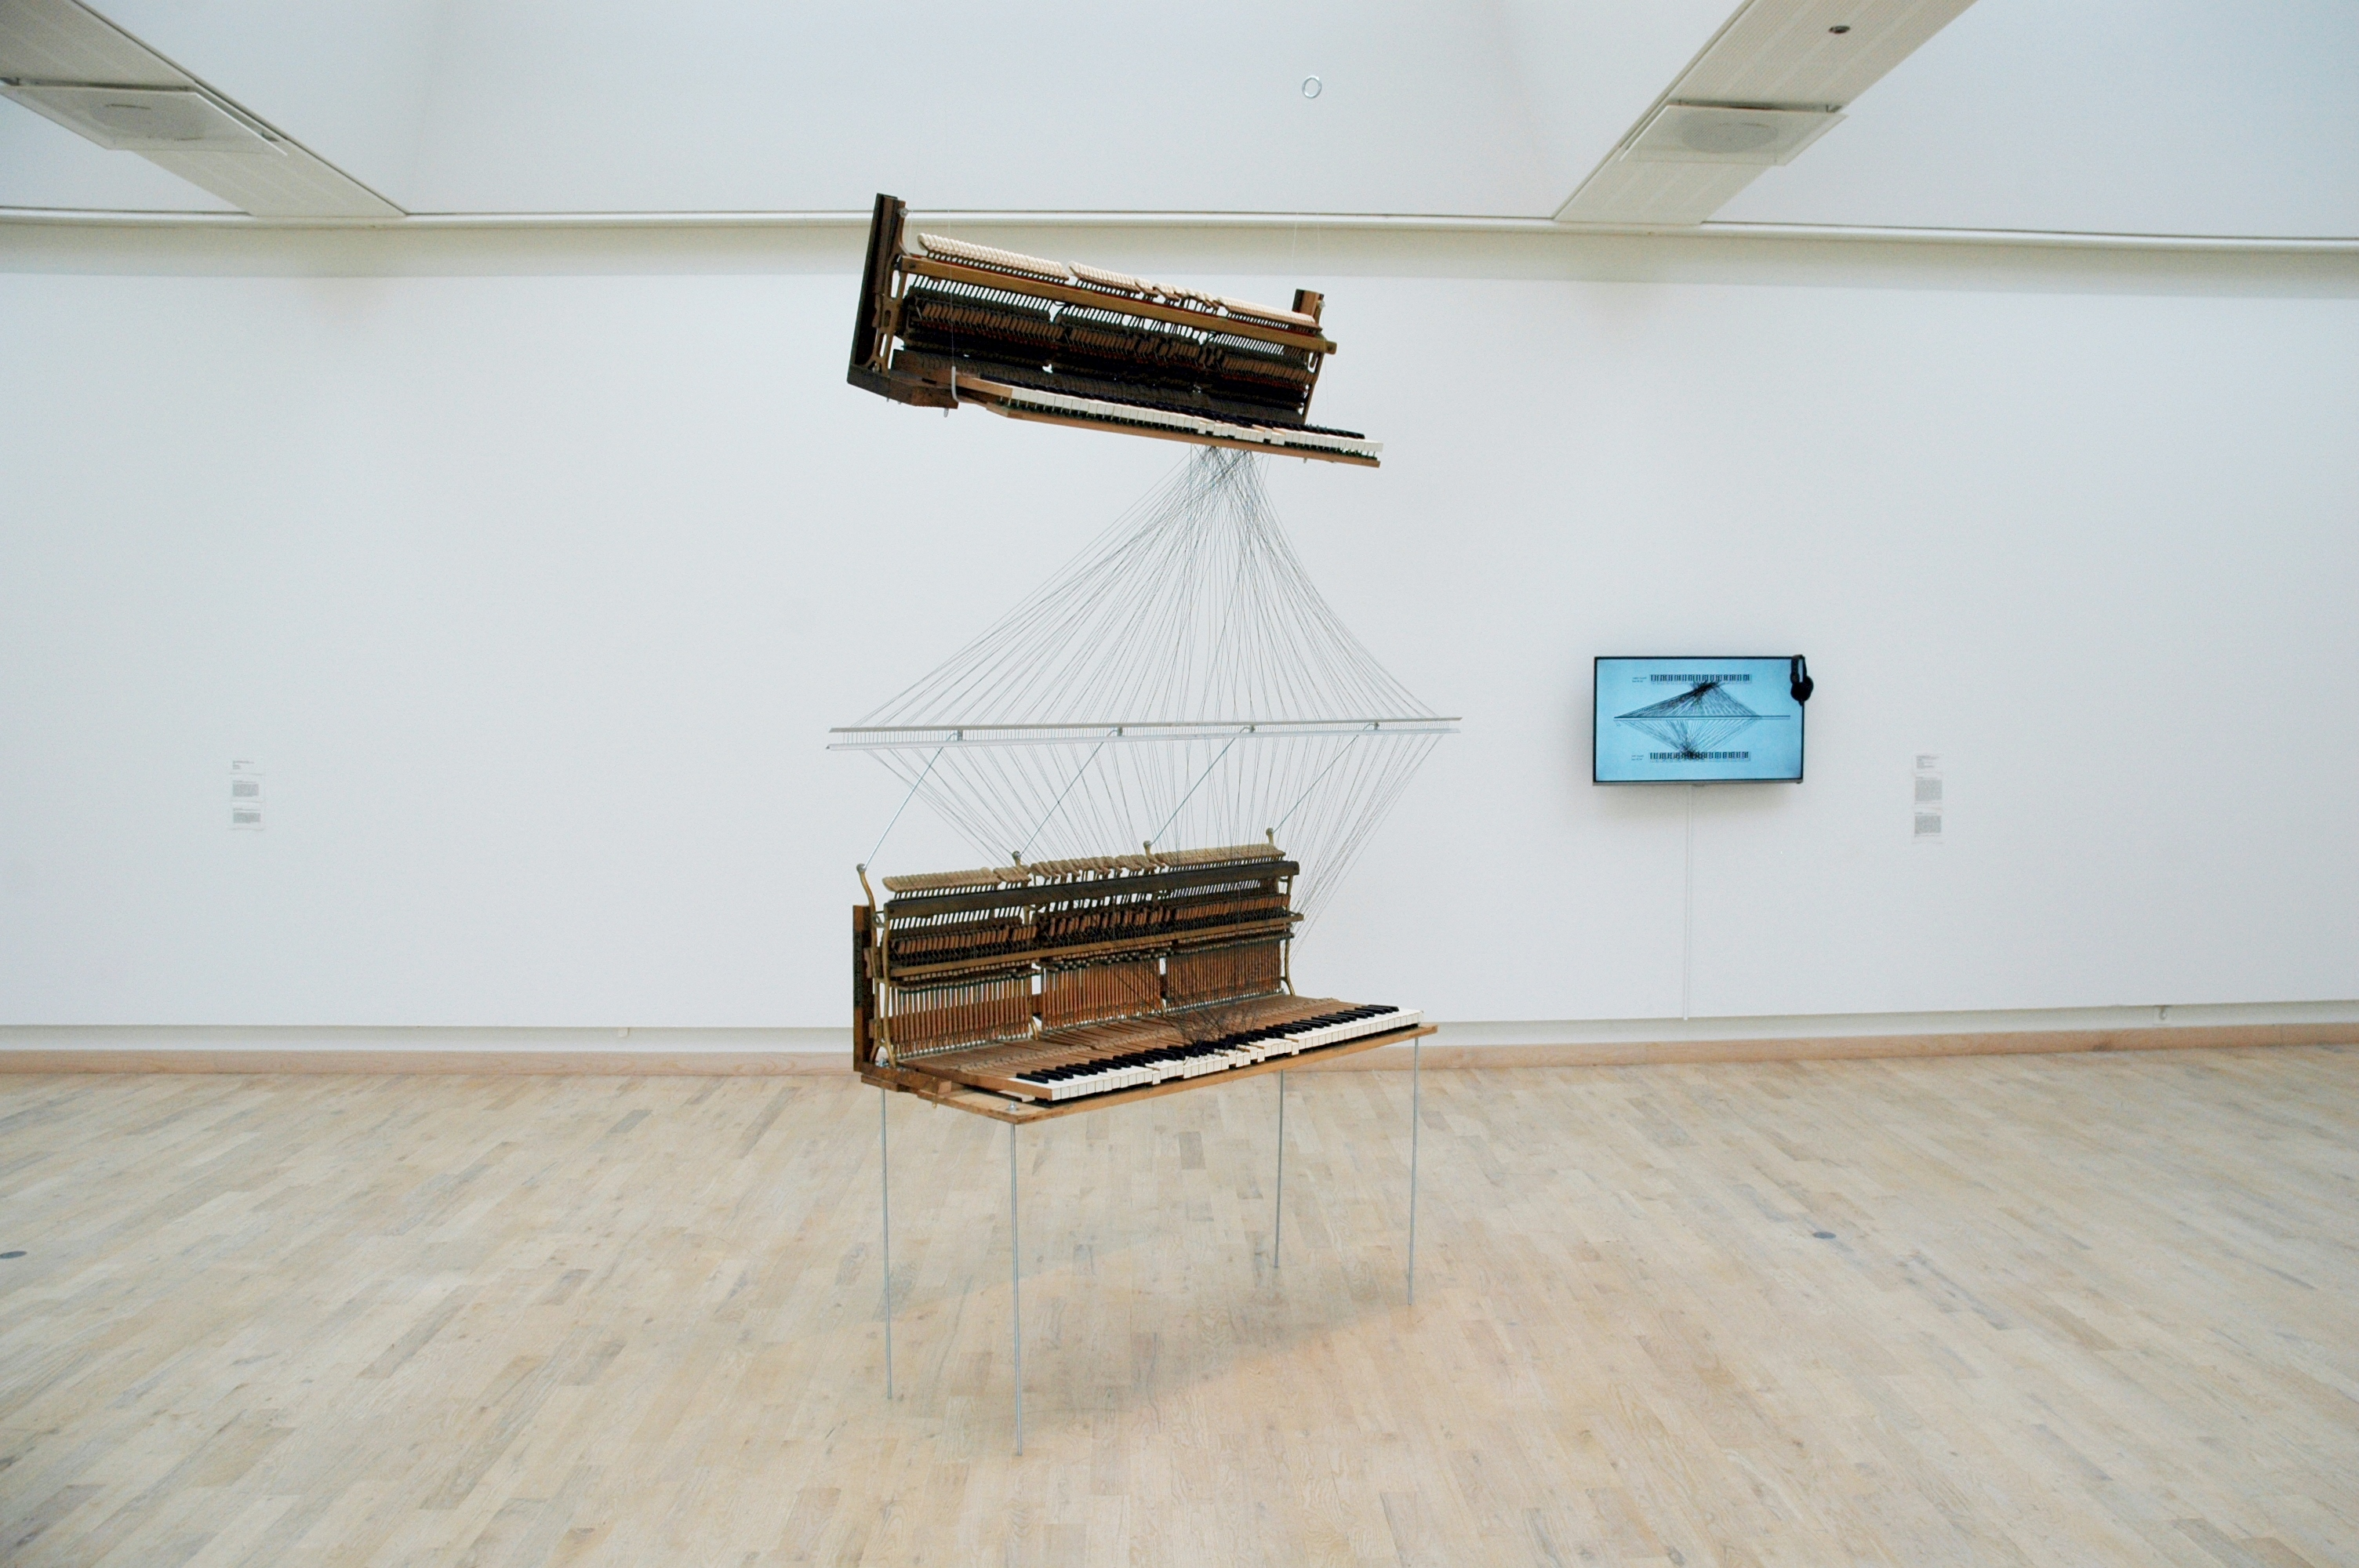
\includegraphics[width=\textwidth]{gfx/Einarson-SchumannSculpture}
	\caption{Einar Torfi Einarsson - Schumann-Sculpture (remnants + deracination)}
	\label{fig:gesture:einarsson}
\end{figure}


\iquote{Every music performance is a dramatic presentation for listeners and improvisers alike. In a sense, both groups play interactive roles as actors from their respective platforms. Just as the design of the hall, the stage and the lighting frames the band's activity for the audience's observation, it also frames the audience's activity for the band to observe. Performers and listeners form a communication loop in which the ction of each continuously affect the other.} Paul F. Berliner in \cite{berliner_thinking_2009}


%%%%%%%%%%%%%%%%%%%%
%-------------------------------------------
\subsection*{Dans les instruments numériques}


Les \glspl{DMI} ont souvent été analysés en tant qu'\gls{IHM}, et les conférences académiques qui leur sont consacré reflètent une culture dans laquelle l'interaction s'exprime via un cahier des charges préalablement identifié: une \gls{IHM} est utilisée dans le cas d'une tâche précise et sa qualité (ergonomie, précision, etc.) peut être mesurée de manière quantifiée.
Dans le cas des instruments de musique cependant, cette tâche est plus complexe, car les enjeux de la création musicale dépassent par essence tout objectif identifié et mesurable au préalable. Par ailleurs, les \glspl{DMI} sont destinés à plusieurs types "d'utilisateurs" ayant un rôle différent : le musicien qui joue de l'instrument, mais également le public, qui bien qu'il ne joue pas de l'instrument est amené à en observer la performance.

Low entry fee, high ceiling.

La performance musicale est un "jeu" qui comporte une part de duplicité. Le public d'un concert est toujours le sujet d'une illusion. 

Un des biais de la littérature sur l’affordance des instruments de musique numérique est qu’elle s’inspire souvent des objectifs de l’affordance des IHM en général, avec l’idée que l’instrument doit être compréhensible pour les “autres” utilisateurs potentiels que l’auteur de l’instrument. Pourtant, nombre d’instruments présentés dans la communauté NIME ne sont joués que par leurs auteurs (cf. [1], [2], [3]) et si le fait de vouloir transmettre son instrument aux autres est louable, il n’est pas gage de qualité en ce qui concerne la création qui sera faite avec cet instrument. 


L'art musical procède en partie de la magie et de l'illusion perceptive. Le musicien nous fait entendre des continuités (e.g. une mélodie) là où l'acoustique fait apparaitre une série discrète (e.g. des notes de piano), ou inversement des fissions (e.g. deux voix indépendantes) là où est jouée une série temporelle de notes sur un même instrument. (=> plutôt que des exemple entre parenthèse, mettre une figure illustrant fission e.g. Bach's Violin Partita No. 3, BWV 1006.)

Cette question du jeu entre le continu et le discret dépasse le seul cadre de la musique mais semble trouver dans cet art de nombreuses espaces d'expression.

Les théories de la perception, en particulier du Gestalt, viennent en partie expliquer les mécanismes qui pousse notre perception à créer des continuités où il n'en existe pas physiquement et inversement à catégoriser des événements selon certaines distances perceptives qui ne sont pas nécessairement en lien avec l'unité de source de production du son.

Si donc on analyse le geste musical, il faut nécessairement prendre en compte sa dimension subversive en ce qu'elle se traduit, particulièrement dans le cas des \glspl{DMI} et des productions musicales impliquant l'électronique en général, dans le design des instruments et outils qui servent à la créer.

\cite{bin_show_2018}

Une étude de Tsay \cite{tsay_sight_2013}, dans laquelle des amateurs et experts sont amenés à évaluer une performance musicale sur la seule base d'un enregistrement silencieux, met en évidence le rôle considérable du la part visuelle dans l'appréciation et l'évaluation de la performance.

Carte et guide , frettage adaptatif (cite \cite{goudard_playing_2014})


\iquote{De même, pour un violoniste, la manière dont il lève le bras et dont il va attaquer le son, la rapidité avec laquelle il prépare son coup d’archet nous renseignent un petit peu, mais pas complètement – parce que l’on ne sait pas quelle hauteur il va jouer – sur certaines catégories du son, comme le fait que le son sera agressif, fort, ou délicat et très doux. (...) Dans la musique instrumentale, cette causalité est très importante car cela participe de la façon dont nous la percevons et l’intérêt, avec la musique électronique, c’est que l’on peut remettre en question cette causalité-là : un tout petit geste peut provoquer une tempête. Entre le geste du pianiste qui va appuyer sur une touche du piano et le son qui va sortir, il y a une machine que j’appelle une boîte noire, qui peut inverser les polarités, c’est-à-dire que je peux très bien programmer la machine de manière à ce que plus le son qui va être joué va être minime, pianissimo, plus le son électronique qui va sortir va être au contraire démesuré : dans ce cas-là, le geste ne correspondra pas du tout au son.} Philippe Manoury interviewé par Anne-Sylvie Barthel-Calvet. (\url{https://geste.hypotheses.org/364})

Dans en Echo de Manoury, ce sont les formants de la voir qui contrôlent la partie électronique, c'est-à-dire un geste invisible, sans contact. (extensible au suivi de partition)


Pouvoir transformer tout type de donnée en geste programmé.


L'interface sensible\footnote{Sur la notion d'interface sensible, cf. \ref{ch:interfaces}} doit pouvoir se prêter à des gestes sans intention, c'est-à-dire qu'elle doit permettre des gestes non-réfléchi, mal-contrôlé ou plutôt in-controlés, qui peuvent tomber en dehors de la zone prévue pour capter de le geste, où d'une manière inadéquate. Cela ne signifie pas nécessairement que l'instrument doit ``faire quelque chose'' de ces gestes: il peut les ignorer.  Mais il est utile que l'intrument permette aux gestes de ``déborder'' du cadre prévu pour leur interaction (si toutefois ce cadre existe).


%-------------------------------------------
\subsection*{Tout ce qui bouge n'est pas geste - partie à revoir ou distribuer}

Dans le domaine de la recherche musicale, les mouvements du corps sont associés à la notion de \textit{geste musical}, c'est-à-dire à un concept associant à la fois le \textit{mouvement} du corps et \textit{l'intention} et/ou \textit{la signification} de ce mouvement. 

Cela n'est pas nécessairement et systématiquement le cas et les mouvements de l'instrumentiste peuvent être envisagés et décrits avec d'autres perspectives que celle de leur potentielle intention. \todo{ref ou footnote ici vers des études en ce sens} La notion de \textit{geste musical} semble en effet implicitement suggérer un rapport hiérarchique entre le musicien et son instrument, dans lequel les gestes ne serait produits qu'intentionnellement, à l'initiative du musicien. Les instruments de musique, et en particulier les DMIs, sont envisagés plus récemment comme \textit{agents} qui opèrent dans un système de relations multi-directionnelles\todo{ref}, que Berliner décrit métaphoriquement par une \textit{conversation} dans \cite{berliner_thinking_2009}. \todo{attention,il parle de la relation musicien/public} 

\Pierre{ je doute qu'il y ait beaucoup de gestes non-intentionnels chez le musicien !}


Les gestes du musicien ne sont pas nécessairement remplis d'une intention ou d'une signification \textit{a priori}, ils peuvent s'apparenter aux gestes de la danse.




L'instrument vibre et produit parfois du son sans qu'il soit explicitement déclenché ou controlé. Les mouvements du corps du musicien en témoignent et au dela des effets spectaculaires des DJs qui touchent aux potentiomètres de leurs interfaces comme s'ils étaient brûlants \footnote{Mark J. Butler apelle \iquote{passion of the knob} (\textit{la fièvre du potentiomètre}) ces moments qui surviennent \iquote{lorsqu'un musicien dirige une expressivité exceptionnellement intense vers un petit composante technique associée à l'ingénierie du son} \cite{butler_playing_2014} \url{https://www.youtube.com/watch?v=Nh9C7nQHmII}}, le corps est parcouru de mouvements qui ne sont pas uniquement des \textit{actions} mais des \textit{réactions} à ce qui est produit par l'instrument. 

\Pierre{ l'exemple choisi devrait être un peu plus analyser car les mouvements du DJs sont probablement totalement intentionnels - c-a-d ils font partie du spectacle car le DJ se sait regardé.}
\Pierre{ je crois plus en la séparation geste-signe et geste-action}

Si l'on considère la relation geste/instrument/musique comme un réseau multi-directionnel, le geste peut-être provoqué par la musique, via l'instrument lui même. Deux exemples caricaturaux viennent illuster cette possibilité : la performance \iquote{eletric stimulus to face — test} de l'artiste Daito Manabe\footnote{\url{http://www.daito.ws/work/electricstimulustoface_test.html}} ou dans le système de motorisation des doigts pour apprendre un instrument proposé récemment à la conférence NIME par \cite{zhang_adaptive_2019}.


Notons enfin que les mouvements peuvent survenir également en interaction avec le public\footnote{This reveals that passion-of-the-knob moments and other actions are not interior to the musician’s world, but rather are intensely meaningful communications: they reverberate outward to the audience and then are reflected back to the stage as formative elements of a milieu whose participants seek to actively cultivate and sustain liveness. in \cite{butler_playing_2014}} 



\subsection*{geste d'impression, geste d'expression}
Si le geste peut ex-primer, c'est-à-dire ``faire sortir en pressant'', un mouvement intérieur et le faire exister dans la temporalité de la performance, il peut aussi im-primer (faire rentrer, en pressant) ce geste sur un support à même d'en accueillir la trace.

geste du latin gero qui signifie ``porter''

S'il y a différance (ajournement et différence) dans la grammatisation musicale (la composition, la lutherie, la programmation), il y a enfin le moment de sa performance, de sa répétition.

Classification des controleurs gestuels dans \cite{wanderley_controgestuel_1999}:
\vspace{-1em}
\begin{itemize}[noitemsep]
\item \textbf{Instrument-like controllers},where the input device design tends to reproduce each feature of an existing (acoustic) instrument in detail. Many examples can be cited, such as electronic keyboards, guitars, saxophones, marimbas, and so on.
\item \textbf{Instrument-inspired controllers} that although largely inspired by the existing instrument’s design, are conceived for another use [62]. Fig. 3 presents one example of such controller, the SuperPolm violin developed by S. Goto, A. Terrier, and P. Pierrot [63], [64], where the input device is loosely based on a violin shape, but is used as a general device to control granular synthesis. => emprunts variés de formes et de fonctions.
\item \textbf{Extended instruments} are instruments augmented by the addition of extra sensors [58], [65]. Commercial augmented instruments included the Yamaha Disklavier, used, for instance, in pieces by J.-C. Risset[66], [67]. Other examples include the flute [68]–[70] and the trumpet [71]–[73], but any existing acoustic instrument may be extended to different degrees by the addition of sensors.
\item \textbf{Alternate controllers} (see, e.g., Fig. 4), whose design does not follow that of an established instrument. Some examples include the Hands [52], graphic drawing tablets [74] (cf. Fig. 5), etc. For instance, an unorthodox gestural controller using the shape of the oral cavity has been proposed in [75].
\end{itemize}

These controllers can furthermore be classified into different categories.
\begin{itemize}[noitemsep]
\item \textbf{Touch, expanded range, or immersive} controllers [76], depending on the amount of physical contact required from the performer. Mulder also [76] separates immersive controllers into internal, external, and symbolic controllers according to the possibilities of visualization of the control surface. In a different approach, Piringer [77] classifies immmersive controllers into partial or completely immersive controllers.
\item \textbf{Individual or collaborativecontrollers}[78],depending on whether the instrument is performed by one or multiple performers at one time.
\item \textbf{Metaphorical} or \item{ad hoc} controllers, and so on.
\end{itemize}


Guerino Mazzola frozen gestures



\iquote{Complétons tout d’abord la phrase : l’ordinateur n’est pas un instrument mais une représentation d’instrument. Cette subtile nuance contient l’essentiel. Envisagé ainsi, l’ordinateur donne une nouvelle dimension au processus de création en y intégrant explicitement, en amont de l’acte instrumental, la construction d’une représentation du dispositif instrumental. Cette construction\/représentation offre une latitude nouvelle : la possibilité pour l’homme de se placer dans une relation ``de type instrumental'', une représentation de relation instrumentale où la liberté d’échapper aux contingences du réel lui permet de créer de nouveaux mondes imaginaires. 
Toutefois, le processus de création est également considérablement transformé par le fait que l’aller\/retour indispensable entre le réel et l’imaginaire, lui aussi, se déplace. Dans le cas de l’instrument réel, l’aller\/retour se fait in situ, dans la relation même avec l’instrument. Dans le cas de la représentation d’instrument, il se fait dans une boucle plus vaste : l’activité de représentation instrumentale, de jeu virtuel, de composition façonnent nos sens et notre intelligence d’une nouvelle manière qui sont alors en jeu dans une perception nouvelle du monde réel... à condition que nous y retournions, c’est à dire que nous ne finissions pas par substituer définitivement nos représentations à la réalité.} \cite{cadoz_musique_1999}, p99.

Claude Cadoz défend l'hypothèse que les appareils électroniques ne sont pas des instruments mais des ``représentations d'instrument''.


 % INCLUDE: interface
% !TEX root = ../thesis-example.tex
%
\chapter{Interfaces sensibles / hardware}
\label{ch:interfaces}

\cleanchapterquote{Komponieren heißt: über die Mittel nachdenken.\\
Komponieren heißt: ein Instrument bauen.\\
Komponieren heißt: nicht sich gehen,\\
sondern sich kommen lassen.}
{Helmut Lachenmann}{1986}
\index[people]{lachenmann@Lachenmann, Helmut}


\cleanchapterquote{Fingers are not to be despised:\\
they are great inspirers, and,\\
in contact with a musical instrument,\\
often give birth to subconscious ideas \\
which might otherwise never come to life.}
{Igor Stravinsky}{\textit{An autobiography}, 1975. \cite{stravinsky_autobiography_1975}}
\index[people]{stravinsky@Stravinsky, Igor}

\vspace*{\fill}

\noindent Dans ce chapitre sont étudiés différents aspects de l'interface des \glspl{DMI}, c'est-à-dire leur part matérielle, tangible et sensible, qui réifie et incarne la part immatérielle et intangible de l'instrument définie par le code informatique, en se situant à la frontière entre ces deux domaines. Seront notamment considérés les éléments concrets qui composent cette interface, le rôle qu'ils y jouent, et la manière dont l'instrumentiste peut appréhender une interface nouvelles.\\
\indent Pour illustrer ces différentes considérations dans un cas pratique, je présenterai également deux interfaces que j'ai développées pour ma pratique musicale : le Filigramophone (figure \ref{fig:interface:filigramophone_unplugged}) et le Xypre (figure \ref{fig:interface:xypre_unplugged}). Ces deux interfaces sont en quelque sorte des variations sur un même archétype d'instrument ``tablette'', nées de l'utilisation initiale d'une tablette graphique Wacom. Leur design reflète les différentes contraintes rencontrées lors du passage d'une technologie à une autre et la manière dont un même modèle général d'interaction est adapté en fonction du médium et des technologies qui l'implémentent et l'incarnent.

\clearpage

%------------ Figure : filigramophone et xypre -----------
\begin{figure}[!htbp]
	\captionsetup{format=plain}%
	\centering
	\begin{minipage}[t]{0.48\textwidth}
		\includegraphics[width=\linewidth]{gfx/05_interfaces/Filigramophone_Overview.jpg}
		\caption[Filigramophone: vue d'ensemble]{Filigramophone, vue d'ensemble du dispositf : Filigramophone, ordinateur avec Max, carte son [sous le] Akai MPD24, haut-parleurs, accessoires de jeu.}
		\label{fig:interface:filigramophone_unplugged}
	\end{minipage}
	\hspace{.02\linewidth}
	\begin{minipage}[t]{0.48\textwidth}
	    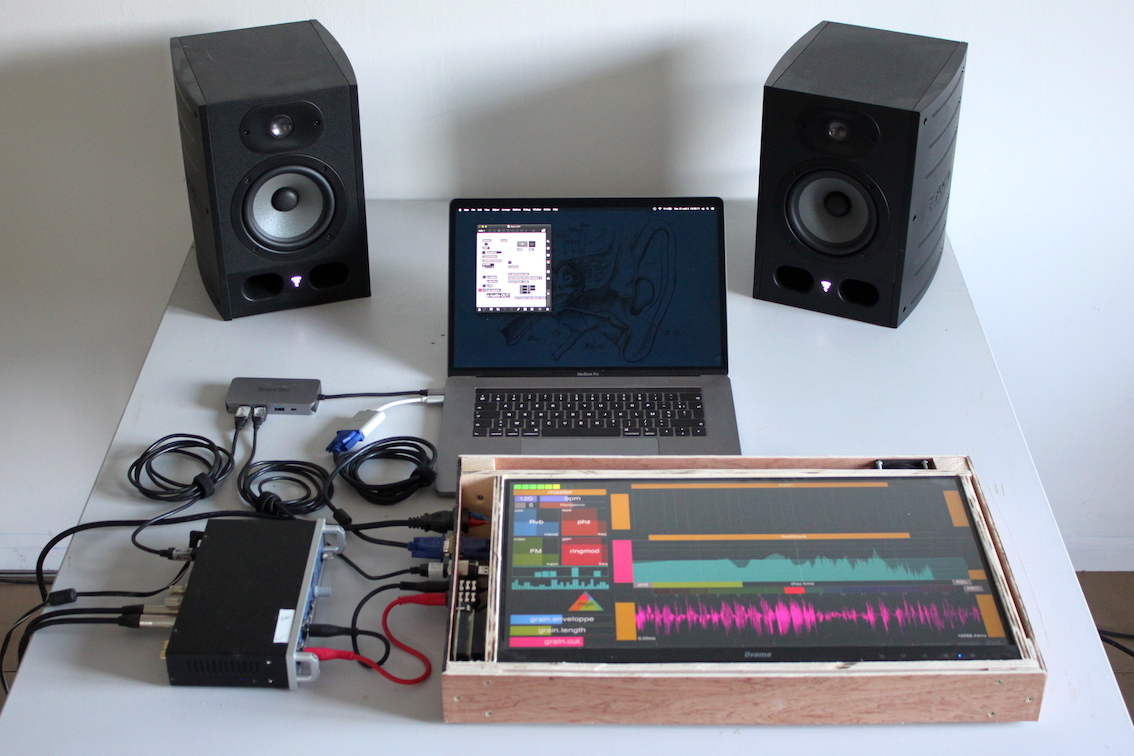
\includegraphics[width=\linewidth]{gfx/05_interfaces/Xypre_Overview_144dpi.jpg}
		\caption[Xypre: vue d'ensemble]{Xypre, vue d'ensemble du dispositif: Xypre, ordinateur avec Max, carte son, haut-parleurs.}
		\label{fig:interface:xypre_unplugged}
	\end{minipage}
\end{figure}
%------------ Figure : filigramophone et xypre piezo -----------

%--------------------------------------------------------------
\section{Différentes faces de l'interface}

\subsection{Interface gestuelle ou interface sensible?}


\noindent Il est souvent question ``d'interface gestuelle'', voire de ``contrôleur gestuel'', lorsqu'on évoque les \glspl{IHM} utilisées pour l'interaction musicale. Comme nous l'avons vu au chapitre précédant, le geste y occupe une part importante, mais les interfaces de jeu ne 
%captent pourtant pas directement le geste, seulement ses éventuels effets sur différents types de capteurs. Ces capteurs peuvent impliquer un contact physique, tels les \gls{FSR} ou les potentiomètres qui constituent les capteurs les plus fréquemment utilisés sur les interfaces. Ces capteurs sont sensibles à des variations physiques telles que 
se limitent pas nécessairement à la captation du geste\footnote{Il serait plus exact de dire qu'elle ne captent pas les gestes, mais les effets des gestes sur les capteurs.} : elle peuvent être sensibles au son\footnote{L'utilisation de microphones est courante et sera développée en particulier dans la section \ref{sec:interfaces:part_acoustique}}, à la température, la lumière\footnote{Voir par exemple les œuvres \textit{Light Thing} de Leafcutter John\index[people]{leafcutterjohn@Leafcutter John (Burton, John, alias—)!lightthing@\textit{Light Thing}} (\url{https://youtu.be/2jIlLHfSEfs}), ou encore \textit{Light Music} de Thierry de Mey\index[people]{mey@de Mey, Thierry!lightmusic@\textit{Light Music}}.}, la couleur, la géolocalisation\footnote{Voir en particulier les travaux d'Atau Tanaka \cite{tanaka_mobile_2004}, ou les instruments de Yann Seznec \url{https://www.impracticaldevices.com}}, aux signaux biologiques internes du corps\footnote{Voir notamment les travaux de Marco Donnarumma\index[people]{donnarumma@Donnarumma, Marco} \cite{donnarumma_biophysical_2017}} et réagir de manière générale à différentes conditions environnementales. Par ailleurs, le geste possède un certain nombre de qualités qui ne sont pas forcément captées par l'interface, alors qu'elles sont effectivement perçues par le musicien et par le public et contribuent ainsi à la performance.\\
\indent Enfin, le ``geste'' qui vient contrôler les processus sonores dans les \glspl{DMI} peut être de nature virtuelle, prendre la forme de motifs pré-enregistrés qui peuvent être issus de toutes sortes de sources de données interprétées en tant que flux temporels, comme c'est le cas dans la ``sonification de données''\footnote{La sonification de données consiste à transformer des données non-sonores, par exemple le cours de la bourse, en signaux audio. Cette technique est notamment utilisée, en dehors du champ musical, pour rendre perceptible des phénomènes ignorés, en s'appuyant en particulier sur nos capacités auditives à identifier des périodicités ou des intervalles de valeurs.} ou l'utilisation de ``modèles intermédiaires''\footnote{La notion de ``modèle intermédiaire'' sera décrite plus en détail dans le chapitre \ref{ch:algorithms}.}. Pour toutes ces raisons, il semblerait ainsi préférable de parler d'\textit{interface sensible}, plutôt que d'\textit{interface gestuelle} pour décrire les dispositifs d'interactions numériques pour la musique, leur caractéristique commune étant l'usage de capteurs (\textit{sensors}).\\
\indent Inversement, les haut-parleurs, les projections graphiques, les moteurs et actionneurs contrôlés algorithmiquement sont également \textit{à l'interface}, en ``sortie'' cette fois, entre le virtuel et le réel. Si de même, on considère plus souvent la partie ``captation'' que la partie ``diffusion'' lorsqu'on évoque les interfaces de jeu des \glspl{DMI}, il faut garder en vue que ces deux aspects s'entremêlent, non seulement dans la boucle d'interaction qui se créé entre le musicien et l'instrument, mais également dans l'agencement concret des éléments matériels qui constituent le dispositif instrumental dans son ensemble, comme nous le verront dans ce chapitre.\\
\indent L'interface de jeu, en étant à la fois sensible à son environnement tout en rendant perceptible les artefacts générés par les algorithmes, traduit dans le réel la potentialité virtuelle d'un \gls{DMI}.


%%%%%%%%%%%%%%%%%%%%%%%%%%%%%%%%%%%%%%%%%
\subsection{Un support pour \textit{musiquer}?}

\noindent Les \glspl{DMI} sont des objets techniques dont l'interface est le support de diverses activités musicales: composition, interprétation, improvisation, pédagogie... En tant qu'agencements éphémères en perpétuelle évolution, leur interface est parfois le support de l'activité même de lutherie qui sert à les concevoir\footnote{L'exemple le plus manifeste de cette amalgame entre les fonctions d'instrument de performance, de composition et de lutherie est sans doute le \textit{live-coding}, dans lequel le clavier alphanumérique (ainsi que l'écran et les haut-parleurs) joue le rôle d'interface de jeu polyvalente pour ces différents contextes.}.\\
%\todo{raccorder la suite avec ce début, e.g. virer ce paragraphe ?}
%\indent Ils intègrent par ailleurs des matériaux pré-composés, que le musicien peut déclencher et qui pourront tourner de manière autonome (paysages sonores, processus génératifs, drones, etc.) et une part créée plus directement, qu'elle soit synthèse ou transformation de matériaux.\\
\indent Par ailleurs, le degré d'interaction du musicien varie du simple déclenchement de processus autonomes jusqu'au contrôle direct et continu de tous les paramètres d'un processus de synthèse sonore.
%\indent Les différents accès de l'interface de jeu doivent ainsi permettrent d'articuler ces différents pôles, en permettant la gestion du temps à différentes échelles. En particulier, les écrans \textit{multitouch}, s'ils permettent de gérer aisément de multiples processus lents (qu'on pourra visualiser et ajuster à l'écran), ne permettent guère une réactivité ``percussive'', telle que le permet un pad \gls{MIDI} ou un capteur échantillonné à fréquence audio.\\
La granularité du contrôle joue un rôle important dans cette perspective. Entre une note \gls{MIDI} qui ne déclenche qu'un événement ponctuel, un contrôleur continu qui envoie des données chaque fois qu'il est modifié et un capteur échantillonné à fréquence audio, qui envoie ses valeurs 44~100 fois par seconde, les possibilités de contrôle seront différentes en terme de réactivité et de finesse de modulation. Il faut donc prévoir les capteurs adéquats pour les processus que l'on souhaite contrôler en aval. Comme le faisait remarquer Max Mathews: \iquote{Il faut penser aux systèmes dans leur globalité pour obtenir quelque chose d'utilisable musicalement - on ne peut pas vraiment développer un capteur sans le mettre en perspective des programmes avec lesquels on va l'utiliser}\footnote{``One has to think of overall systems to get a musically useful thing — you can't really develop a sensor without relating it to the programs that you're going to use it with.'', Max Mathews, cité par Joel Chadabe dans \cite{chadabe_electric_1996}, p. 230}.\\
\indent Ceci n'est pas sans poser problème dans la perspective de modularité d'un \gls{DMI} que l'on aimerait pouvoir faire évoluer et adapter à différents contextes, différents projets. Une direction consiste à disposer d'une palette de capteurs variés, afin de les agencer selon une ergonomie adaptée aux gestes qu'ils invitent, et d'adapter le logiciel, plus souple, à cette configuration\footnote{C'est par exemple la direction prise dans le Méta-Instrument de Serge de Laubier, qui peut charger toute une série d'instruments logiciels différents (cf. \cite{couprie_meta-instrument:_2018}).}. Une autre direction, sans compromission de l'interface, consiste à accepter le fait qu'un instrument ne puisse pas tout faire et à prendre l'objet tel quel, dans sa complexité, avec ses résistances, avec ses choix esthétiques, avec son usage unique et singulier\footnote{C'est par exemple davantage le cas dans \textit{The Sponge} de Martin Marier\index[people]{marier@Marier, Martin} (figure \ref{fig:interface:TheSponge}).}. 

\subsection{Instruments acoustico-électronico-numériques}

\noindent Si on les considère sur le plan matériel, il faut encore noter que les \glspl{DMI}, s'ils se caractérisent par l'usage de la computation numérique, sont aussi nécessairement des instruments électroniques, électriques et acoustiques. Il portent par conséquent l'héritage et les contraintes propres à ces différentes dimensions.\\
\indent Dans le domaine virtuel du code informatique, ces dimensions sont (trop\footnote{Cf. commentaires en section \ref{ch:algorithms:digital-material}.}) bien séparées : la mécanique et l'électricité y sont absentes, et les signaux acoustiques et de contrôle bien rangés dans des variables indépendantes qui n'interagissent que si on le leur demande explicitement. Dans le monde réel, au contraire, l'interférence est la règle --~pour le meilleur et pour le pire~-- et il devient nécessaire d'isoler les différents signaux si l'on ne veut pas avoir à gérer la complexité de leur interaction : mettre les haut-parleurs loin des microphones, isoler les câbles électriques pour ne pas capter la radio, rajouter des mousses pour ne pas entendre les bruits mécaniques d'une frappe sur un capteur, etc. En se situant à la frontière, l'interface de jeu doit communiquer avec le virtuel mais aussi composer avec le réel.

%-------------------------------------------------------------

\subsection{Facteurs de formes: héritages et transpositions}
\label{sec:interfaces:heritages}

\noindent En partie libérée\footnote{En partie seulement, cf. § \ref{sec:interfaces:part_acoustique}} des contraintes de facteur de forme liées à l'acoustique, l'interface de jeu présente un agencement et une topologie liés à des questions d'ergonomie d'une part mais aussi de divers héritages musicaux et extra-musicaux. Il ne s'agit pas ici de juger des directions les plus adaptées à la performance instrumentale, mais de constater leur usage effectif dans ce domaine par les musiciens numériques, en analysant leur intérêt respectif.

\subsubsection{Héritage instrumental}
\label{sec:interfaces:heritages:instrument}
%------------ Figure : Hyvibe et SmartMandolin -----------
\begin{figure}[!htbp]
	\captionsetup{format=plain}%
	\centering
	\begin{minipage}[t]{0.48\textwidth}
		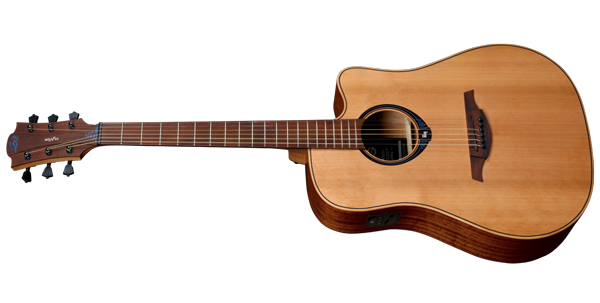
\includegraphics[width=\linewidth]{gfx/05_interfaces/HyVibe-guitar.png}
		\caption[La Smart Guitar de HyVibe]{La Smart Guitar de HyVibe ressemble à s'y méprendre à une guitare. Photographie © HyVibe}
		\label{fig:interface:hyvibe}
	\end{minipage}
	\hspace{.02\linewidth}
	\begin{minipage}[t]{0.48\textwidth}
	    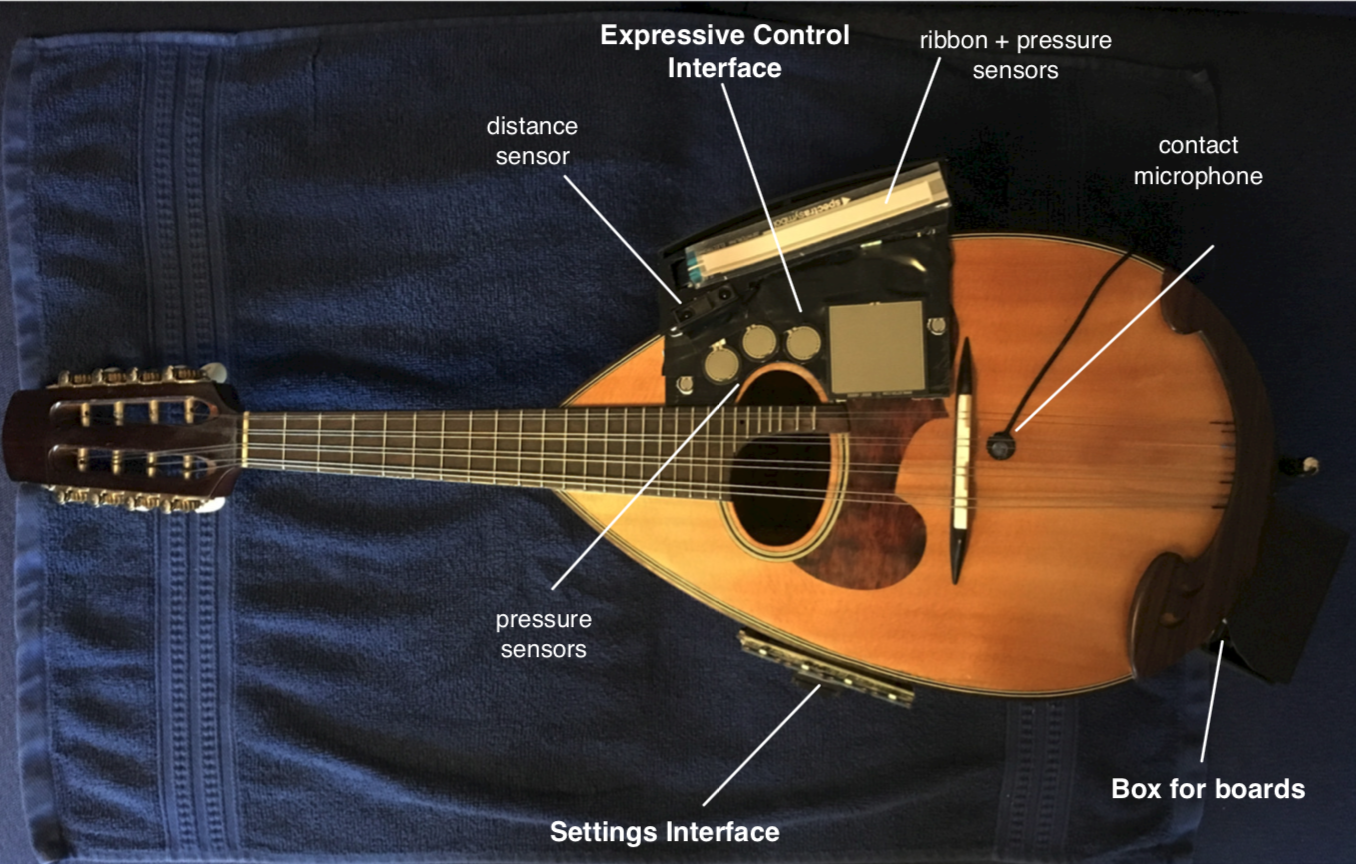
\includegraphics[width=\linewidth]{gfx/05_interfaces/Turchet-SmartMandolin.png}
		\caption[La Smart Mandolin de Lucas Turchet]{La Smart Mandolin de Lucas Turchet, avec capteurs ajouté sur la caisse. Photographie © Lucas Turchet}
		\label{fig:interface:smart-mandolin}
	\end{minipage}
\end{figure}
%------------ Figure : Hyvibe et SmartMandolin -----------
 \noindent L'héritage le plus évident est celui des techniques de jeu et du répertoire, qui prend une importance considérable dans le design des \glspl{DMI} inspirés d'instruments pré-existants, en particulier les instruments dits augmentés (cf. figure \ref{fig:interface:hyvibe} et \ref{fig:interface:smart-mandolin} et annexes \ref{appendix:turchet} et \ref{appendix:mamou-mani}). Cet héritage est le plus manifeste dans les instruments qui se destinent à une diffusion commerciale, en permettant un effet dilligence\footnote{Notion définie par le médiologue Jacques Perriault, décrivant les protocoles mis en place pour l'adaptation d'une innovation en vue de son acceptation sociale (Les premiers wagons avaient la forme des diligences.)} entre instruments classiques et instruments nouveaux\footnote{\label{fn:Pinch}Cf. sur ce sujet l'analyse de Trevor Pinch dans \cite{pinch_why_2001} sur la présence de clavier sur les premiers synthétiseurs et section \label{sec:visual_representation:visual_aspects:adaptation_to_sound}.}.\\
 \indent Outre l'héritage gestuel liés aux modes de jeu sur les instruments acoustiques, les théories de la musique s'inscrivent de manière plus générale dans l'interface de jeu, en imprimant sur elles une topologie polarisée par les valeurs auxquelles elle recourt\footnote{Cf. section \ref{ch:visual_representation:music-theory}} (rythmes, intensités, hauteurs, timbre, etc.).


\subsubsection{Héritage scientifico-industriel}
\vspace{1em}
%------------ Figure : Sponge et Lungta ----------- 
% todo : utiliser subfig pour une légence commune ici ?
\begin{figure}[!htbp]
	\captionsetup{format=plain}%
	\centering
	\begin{minipage}[t]{0.48\textwidth}
		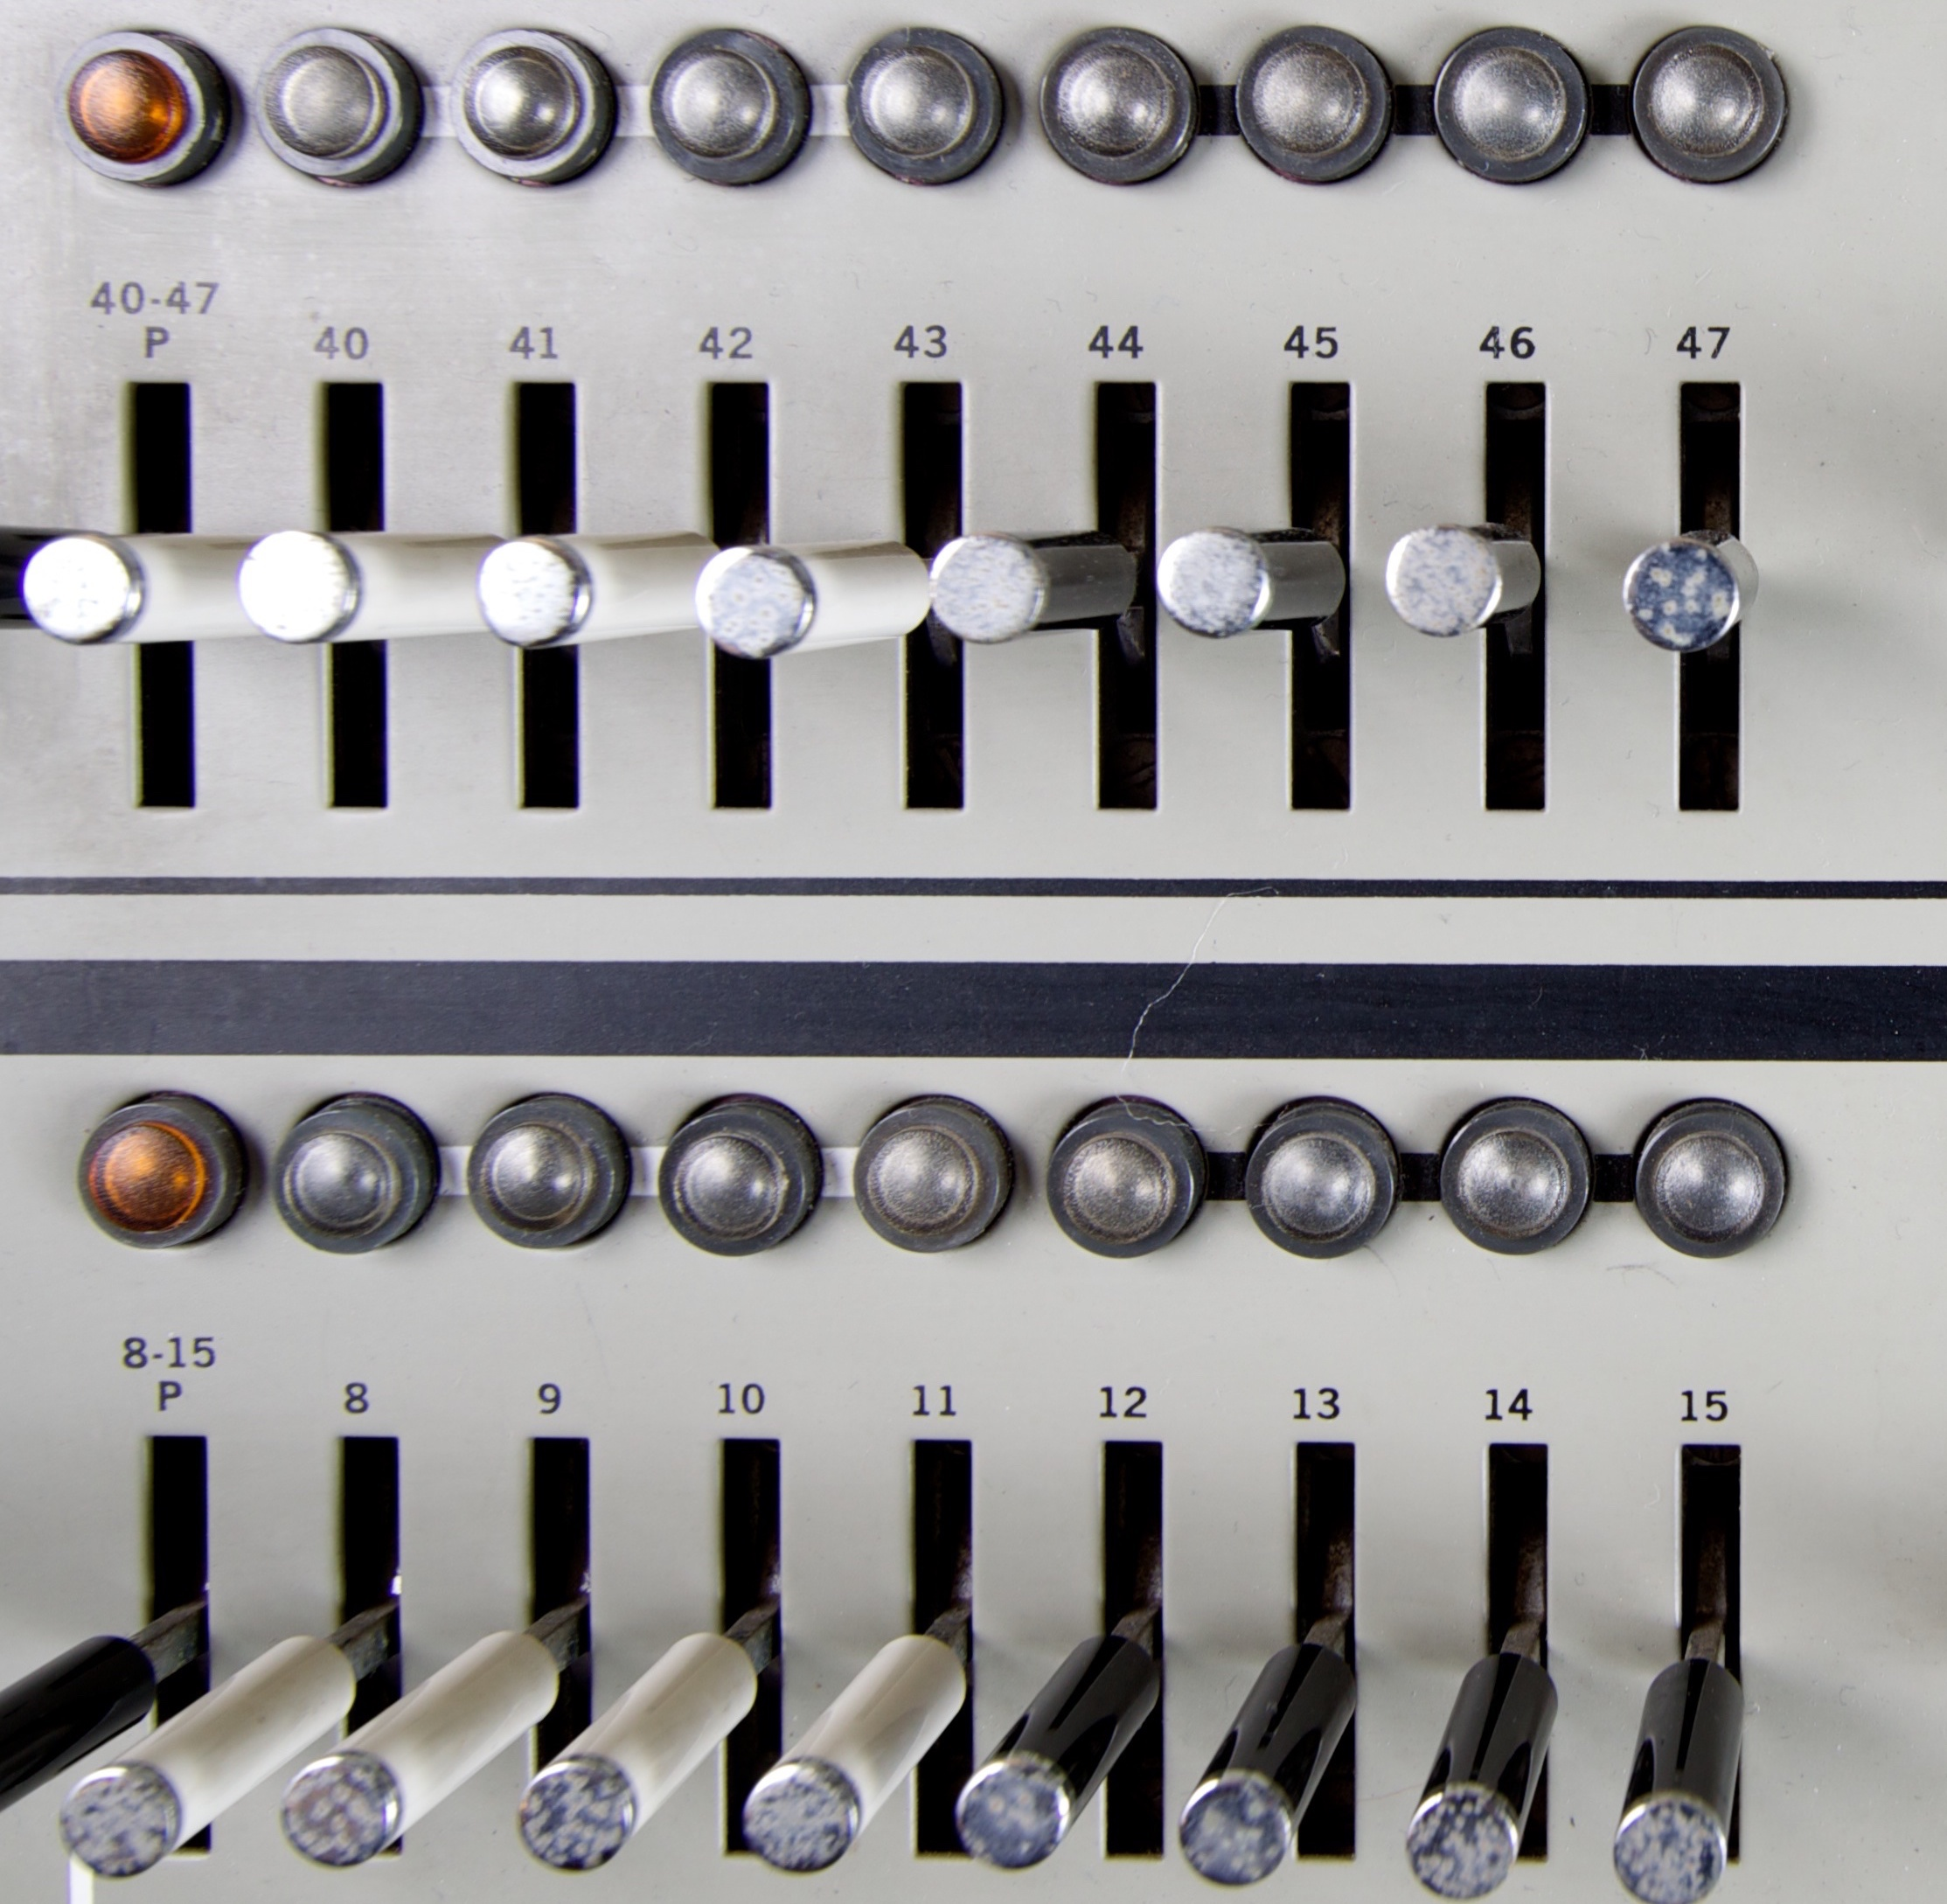
\includegraphics[width=\linewidth]{gfx/05_interfaces/IBM_System_360_Panel.jpg}
		\caption[L'interface du système 360 d'IBM]{Interface du\textit{ Système 360} d'IBM (détail), un ordinateur utilisé dans le domaine scientifique et l'ingénierie, commercialisé en 1965.}
		\label{fig:interface:ibm360}
	\end{minipage}
	\hspace{.02\linewidth}
	\begin{minipage}[t]{0.48\textwidth}
	    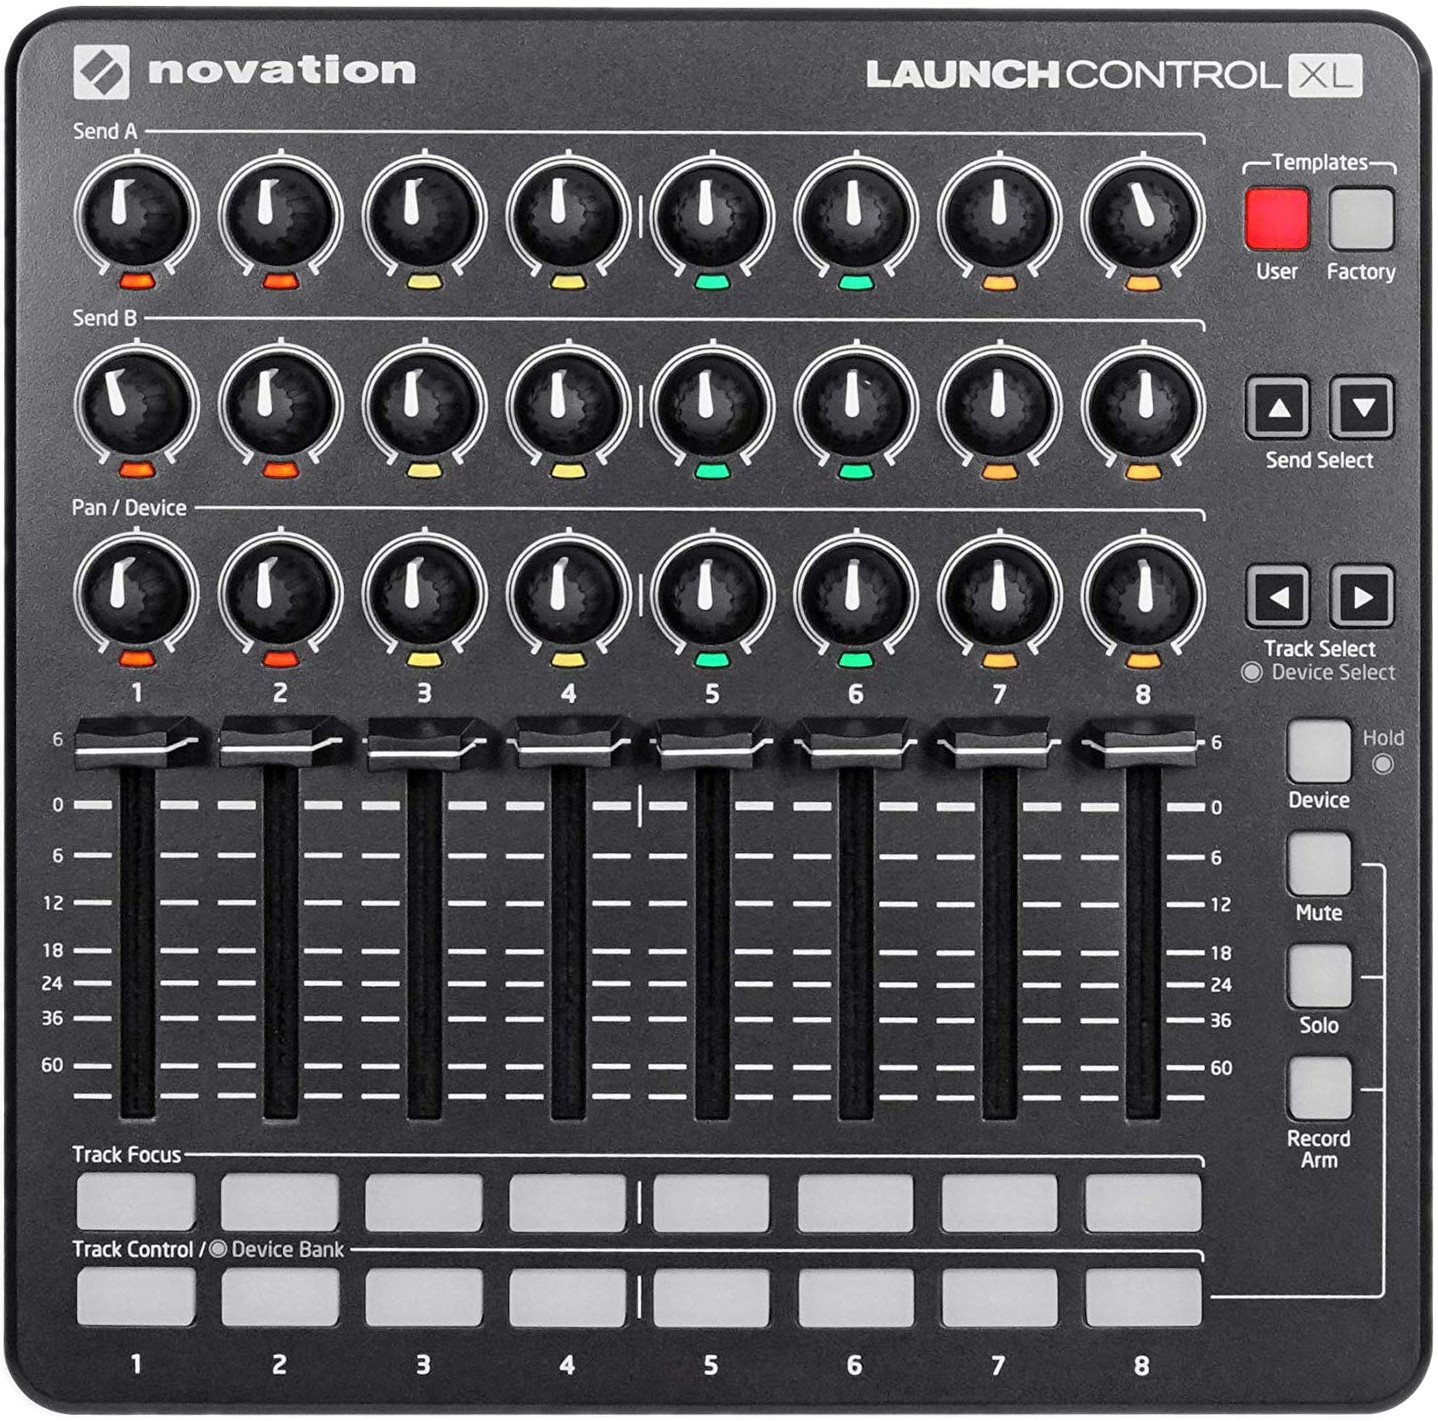
\includegraphics[width=\linewidth]{gfx/05_interfaces/NovationLaunchControlXL.jpg}
		\caption[L'interface MIDI Novation Launch-Control-XL]{Le \textit{Launch-Control XL} de Novation, une interface \gls{MIDI} dédiée à l'expression musicale, commercialisée en 2014.}
		\label{fig:interface:launchpad-controlXL}
	\end{minipage}
\end{figure}

\noindent L'informatique et l'ingénierie électronique, avec leur ancrage historique dans le domaine scientifique, industriel et militaire contribuent également à façonner les interfaces qui héritent des panneaux de commandes garnis de potentiomètres rotatifs, de faders et de LEDs clignotantes disposés en matrices rectilignes (cf. figure \ref{fig:interface:ibm360} et \ref{fig:interface:launchpad-controlXL}). Les interfaces graphiques connaissent le même genre d'influence avec l'héritage de la bureautique (dossiers et fichiers, poubelle, menus déroulants, etc.), omniprésent dans le design des logiciels et parfois imposé\footnote{Par exemple, le non-respect des règles de design édictées par Apple peut entraîner le refus de la publier (même gratuitement) sur l'app store.}. L'intérêt de ces interfaces est de présenter le maximum de contrôleurs indépendants, en facilitant le monitoring par une représentation uniforme adapté à une lecture rapide de leurs valeurs.

\subsubsection{Héritage du corps}

\noindent L'ergonomie, pensée en dehors de l'organologie classique, nous amène à considérer directement le corps, et plus particulièrement les mains. Comme l'explique Serge de Laubier (cf. Annexe \ref{appendix:delaubier}) : \iquote{(...) quand on fabrique un instrument il y a une contrainte, c'est le corps et donc forcément, il faut que les instruments, en tout cas ceux qui fonctionnent bien, soient quand même relativement bien adaptés au corps (...) et la première contrainte c'est celle des mains (...) parce que c'est [le membre] le plus agile, je pense, le plus agile, rapide, réactif.} Un certain nombre d'instruments comme ``The Hands'' de Michel Waisvisz --~dont le nom parle de lui-même~-- ou le Méta-Instrument de Serge De Laubier sont ainsi directement conçus à partir de l'ergonomie de la main.\\
\indent Le corps entier peut être utilisé de manière instrumentale, en particulier dans la domaine chorégraphique. Si les interactions entre la danse et les systèmes électroniques interactifs ont plus de 50 ans\footnote{En 1965, Merce Cunningham, John Cage et David Tudor utilisaient déjà des capteurs photo-électriques pour contrôler les processus musicaux dans la performance \textit{Variation V}.\index[people]{cage@Cage, John!variationv@\textit{Variation V}}\index[people]{tudor@Tudor, David!variationv@\textit{Variation V}}\index[people]{cunningham@Cunningham, Merce!variationv@\textit{Variation V}}}, les interfaces de \textit{motion capture}, devenues plus accessibles depuis le début du \siecle{21}~siècle\footnote{On pense ici aux webcams et aux nouveaux usages permis par les progrès de l'analyse d'image et d'apprentissage, à la Kinect de Microsoft, au Leap-motion, aux capteurs de type \gls{AHRS}, etc.} ont multiplié le nombre de performances chorégraphiques dans lesquelles l'expertise du mouvement corporel est directement utilisée pour le contrôle de processus musicaux\footnote{Voir notamment les créations de Myriam Gourfink et Kasper Toeplitz, et les travaux de Frédéric Bevilacqua, e.g. \cite{bevilacqua_gesture_2011}}.\\
\indent Enfin, les mouvements internes du corps tels que la tension musculaire, les battements du cœur, ou l'activité cérébrale sont envisageables pour l'interaction instrumentale en utilisant des capteurs de signaux bio-physiques (ECG, EEG, EMG, etc.). Une analyse détaillée de cette perspective est proposée par Atau Tanaka et Marco Donnarumma dans \cite{tanaka_body_2019}, qui sont eux-mêmes les auteurs de plusieurs projets et performances musicales dans cette veine.

\subsubsection{Héritage poétique de l'objet}

\noindent C'est parfois l'absence d'héritage instrumental qui est recherchée. Martin Marier\footnote{Voir les vidéos sur \url{http://www.martinmarier.com}} explique ainsi le design de l'interface ``The Sponge'' \cite{marier_sponge_2010} (figure \ref{fig:interface:TheSponge}), dont il souhaite qu'elle ne fasse référence à aucun instrument existant, afin que son apparence ne dicte pas de paradigme musical, ni ne créé d'attente particulière du public en terme de composition.\\
%------------ Figure : Sponge et Lungta -----------
\begin{figure}[!htbp]
	\captionsetup{format=plain}%
	\centering
	\begin{minipage}[t]{0.48\textwidth}
		\includegraphics[width=\linewidth]{gfx/05_interfaces/epongeCloseUp_prestonBeebe.jpg}
		\caption[``The Sponge'' de Martin Marier]{``The Sponge'', une interface instrumentale de Martin Marier. Photographie © Preston Beebe.}
		\label{fig:interface:TheSponge}
	\end{minipage}
	\hspace{.02\linewidth}
	\begin{minipage}[t]{0.48\textwidth}
	    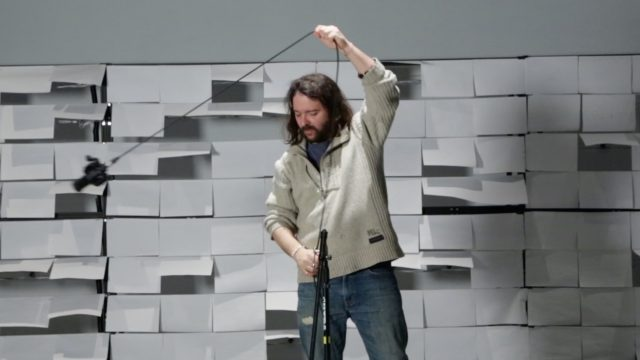
\includegraphics[width=\linewidth]{gfx/05_interfaces/Saint-Denis-Lungta.jpg}
		\caption[LUNGTA de Patrick Saint-Denis]{LUNGTA, une installation performative basée sur une matrice de feuilles de papier controlée algorithmiquement. Photographie © Patrick Saint-Denis.}
		\label{fig:interface:lungta}
	\end{minipage}
\end{figure}
%------------ Figure : Sponge et Lungta -----------
\index[people]{saintdenis@Saint Denis, Patrick!lungta@\textit{LUNGTA}}
\index[people]{marier@Marier, Martin}
\indent L'instrument est également un objet mis en scène et son rôle scénographique vient parfois façonner son instrumentalité. C'est le cas par exemple dans les créations de Patrick Saint-Denis\footnote{Voir les vidéos sur \url{http://www.patricksaintdenis.com}}, qui \iquote{part de l'objet} et \iquote{poursuit l'idée des objets animés par le son} (cf. figure \ref{fig:interface:lungta} et annexe \ref{appendix:saint-denis}).\\
\noindent L'idée d'utiliser la connotation des objets employés comme instruments de musique était également centrale dans la performance audiovisuelle \textit{Donjon}\footnote{Plus de détails sur \url{http://vincentgoudard.com/donjon}} (Cécile Babiole, Jean-Michel Dumas, Vincent Goudard), dans laquelle des bornes d'arcades des années 1980 reconverties, à l'aide d'une électronique \textit{ad hoc}, en interfaces de jeu pour le contrôle de l'image et du son en temps réel, faisaient écho à l'esthétique musicale et visuelle de la performance (figure \ref{fig:interface:donjon}).\\
%------------ Figure : Donjon -----------
% \begin{figure}[!htbp]
% 	\captionsetup{format=plain}%
% 	\makebox[\linewidth][c]{%
% 		\begin{subfigure}[b]{.5\textwidth}
% 			\centering
% 			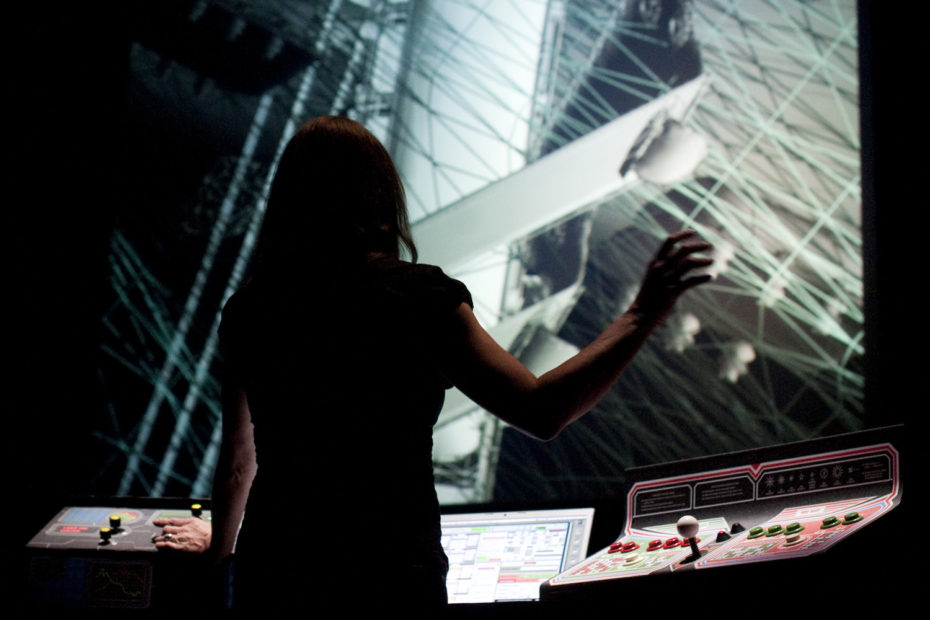
\includegraphics[width=\linewidth]{gfx/05_interfaces/Donjon_Cecile.jpg}
% 			%\caption{Son vers gestes}
% 		\end{subfigure}%
% 		\hspace{.01\linewidth}
% 		\begin{subfigure}[b]{.5\textwidth}
% 			\centering
% 			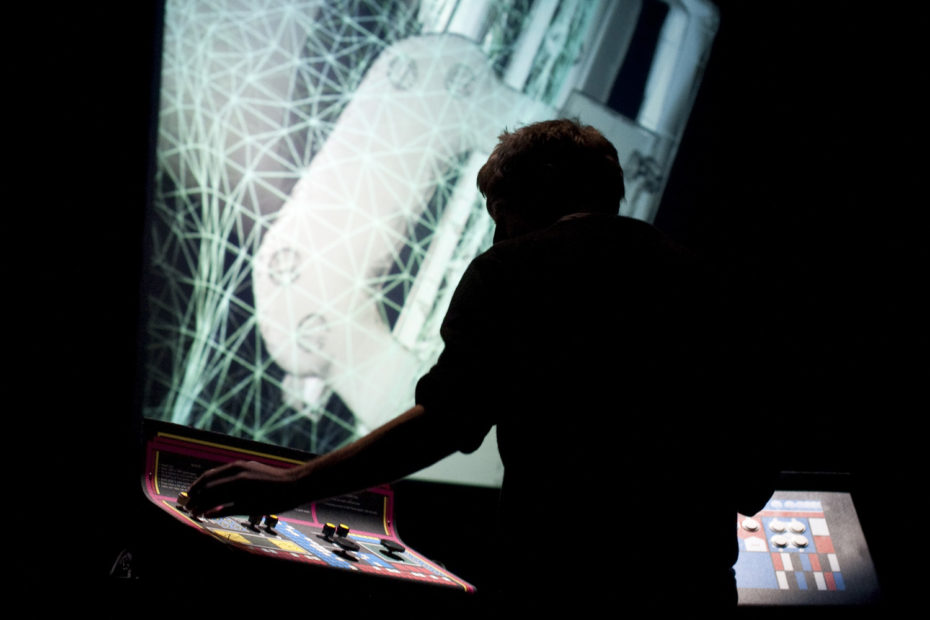
\includegraphics[width=\linewidth]{gfx/05_interfaces/Donjon_Vincent.jpg}
% 			%\caption{Instrument vers gestes}
% 		\end{subfigure}%
% 	}
% 	\caption[Donjon, performance audiovisuelle utilisant des bornes d'arcade]{Des bornes d'arcade, à l'esthétique très connotée années 1980, utilisées comme interface de jeu dans la performance audiovisuelle \textit{Donjon}. À gauche: Cécile Babiole, à droite: Vincent Goudard. Photographie: Sébastien Bozon}
% 	\label{fig:interface:donjon}
% \end{figure}
%------------ Figure : Donjon -----------
%------------ Figure : Donjon -----------
\begin{figure}[!htbp]
	\captionsetup{format=plain}%
	\makebox[\linewidth][c]{%
		\begin{subfigure}[b]{.5\textwidth}
			\centering
			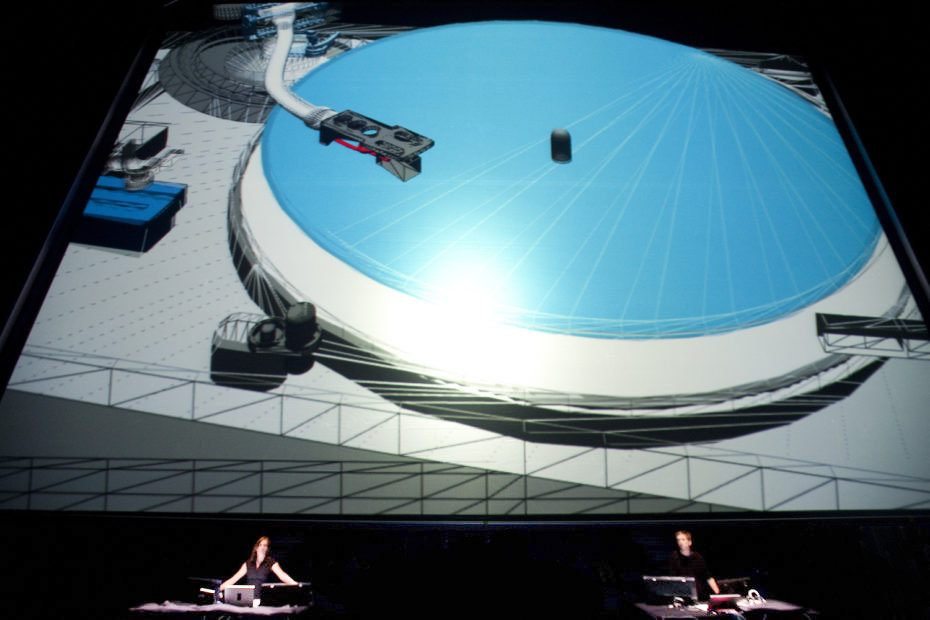
\includegraphics[width=\linewidth]{gfx/05_interfaces/Donjon_Filature2.jpg}
			%\caption{Son vers gestes}
		\end{subfigure}%
		\hspace{.01\linewidth}
		\begin{subfigure}[b]{.5\textwidth}
			\centering
			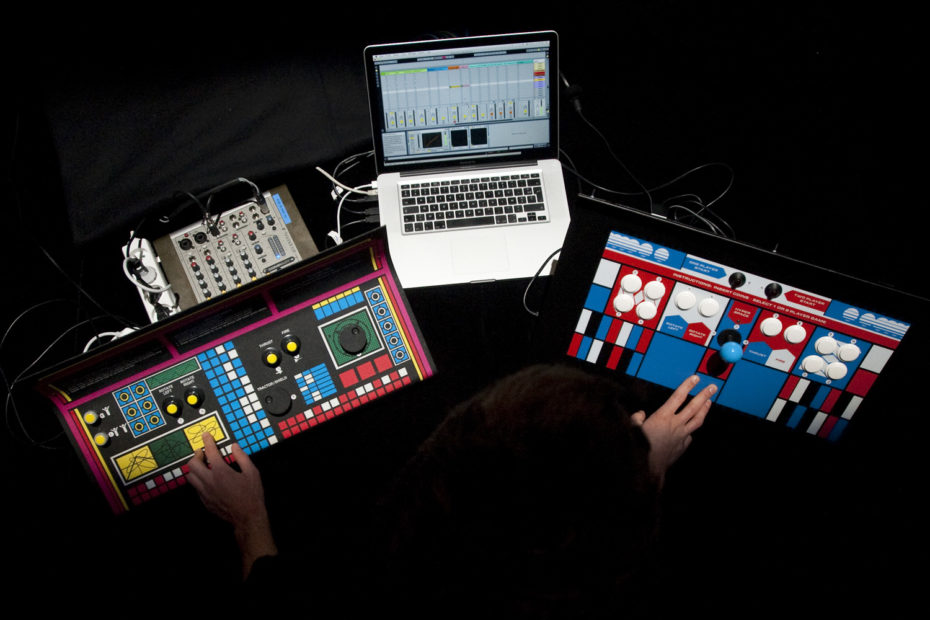
\includegraphics[width=\linewidth]{gfx/05_interfaces/Donjon_Vincent_interfaces.jpg}
			%\caption{Instrument vers gestes}
		\end{subfigure}%
	}
	\caption[Donjon, performance audiovisuelle utilisant des bornes d'arcade]{Des bornes d'arcade, à l'esthétique très connotée, utilisées comme interface de jeu dans la performance audiovisuelle \textit{Donjon}. À gauche: Vue d'ensemble de la scène, à droite: détail des interfaces de Vincent Goudard. Photographies: Sébastien Bozon.}
	\label{fig:interface:donjon}
\end{figure}
\index[people]{babiole@Babiole, Cécile!donjon@\textit{Donjon}}
\index[people]{goudard@Goudard, Vincent!donjon@\textit{Donjon}}

%------------ Figure : Donjon -----------
\indent L'interface est ainsi forgée par la force d'évocation poétique des objets, qui dépasse le strict cadre fonctionnel de la relation instrumentale. La mythologie qui leur est associée polarise le jeu du musicien et l'écoute du public, \iquote{comme s'il y avait un arrière plan imaginaire de tout ce que ça draine d'histoire, de projections} (cf. Annexe \ref{appendix:dumeaux}). On retrouve cette même fonction poétique dans ``l'Olitherpe'', instrument joué par Patricia Dallio\index[people]{dallio@Dallio, Patricia}\footnote{Site web : \url{http://www.patriciadallio.com}. Voir le documentaire ``L'Olitherpe et la teneur de l'air'' (\url{https://vimeo.com/224494409}) à propos des considérations faites ici.}, qui se présente comme un agencement de capteurs intégrés dans des objets de récupération. Les associations morphologiques et fantasmagoriques entre mouvements de l'instrumentiste, fonction des capteurs et forme des objets tient un rôle essentiel dans la construction de l'interface de jeu: par exemple, le capteur infra-rouge évocant des yeux est intégré dans un vieux phare de vélo.\\
\indent On peut voir dans la démarche artisanale et \gls{DIY} des lutheries numériques l`importance accordée à la charge affective de l'instrument; les interfaces numériques (tels que les contrôleurs \gls{MIDI}) vendues dans le commerce sont en effet souvent issus d'une production industrielle et faits de matériaux plastiques qui à l'inverse du bois d'un violon, ne porte pas la trace organique des fibres du bois ou celle du geste artisanal imprimé par le luthier et se retrouve, d'une certaine manière, dépourvu d'histoire.

%%%%%%%%%%%%%%%%%%%%%%%%%%

\section{Matériaux}
\label{sec:interfaces:materials}

%-------------------------- Figure : table du luthier numérique ----------------------------------
\begin{figure}[!htbp]
	\captionsetup{format=plain}%
	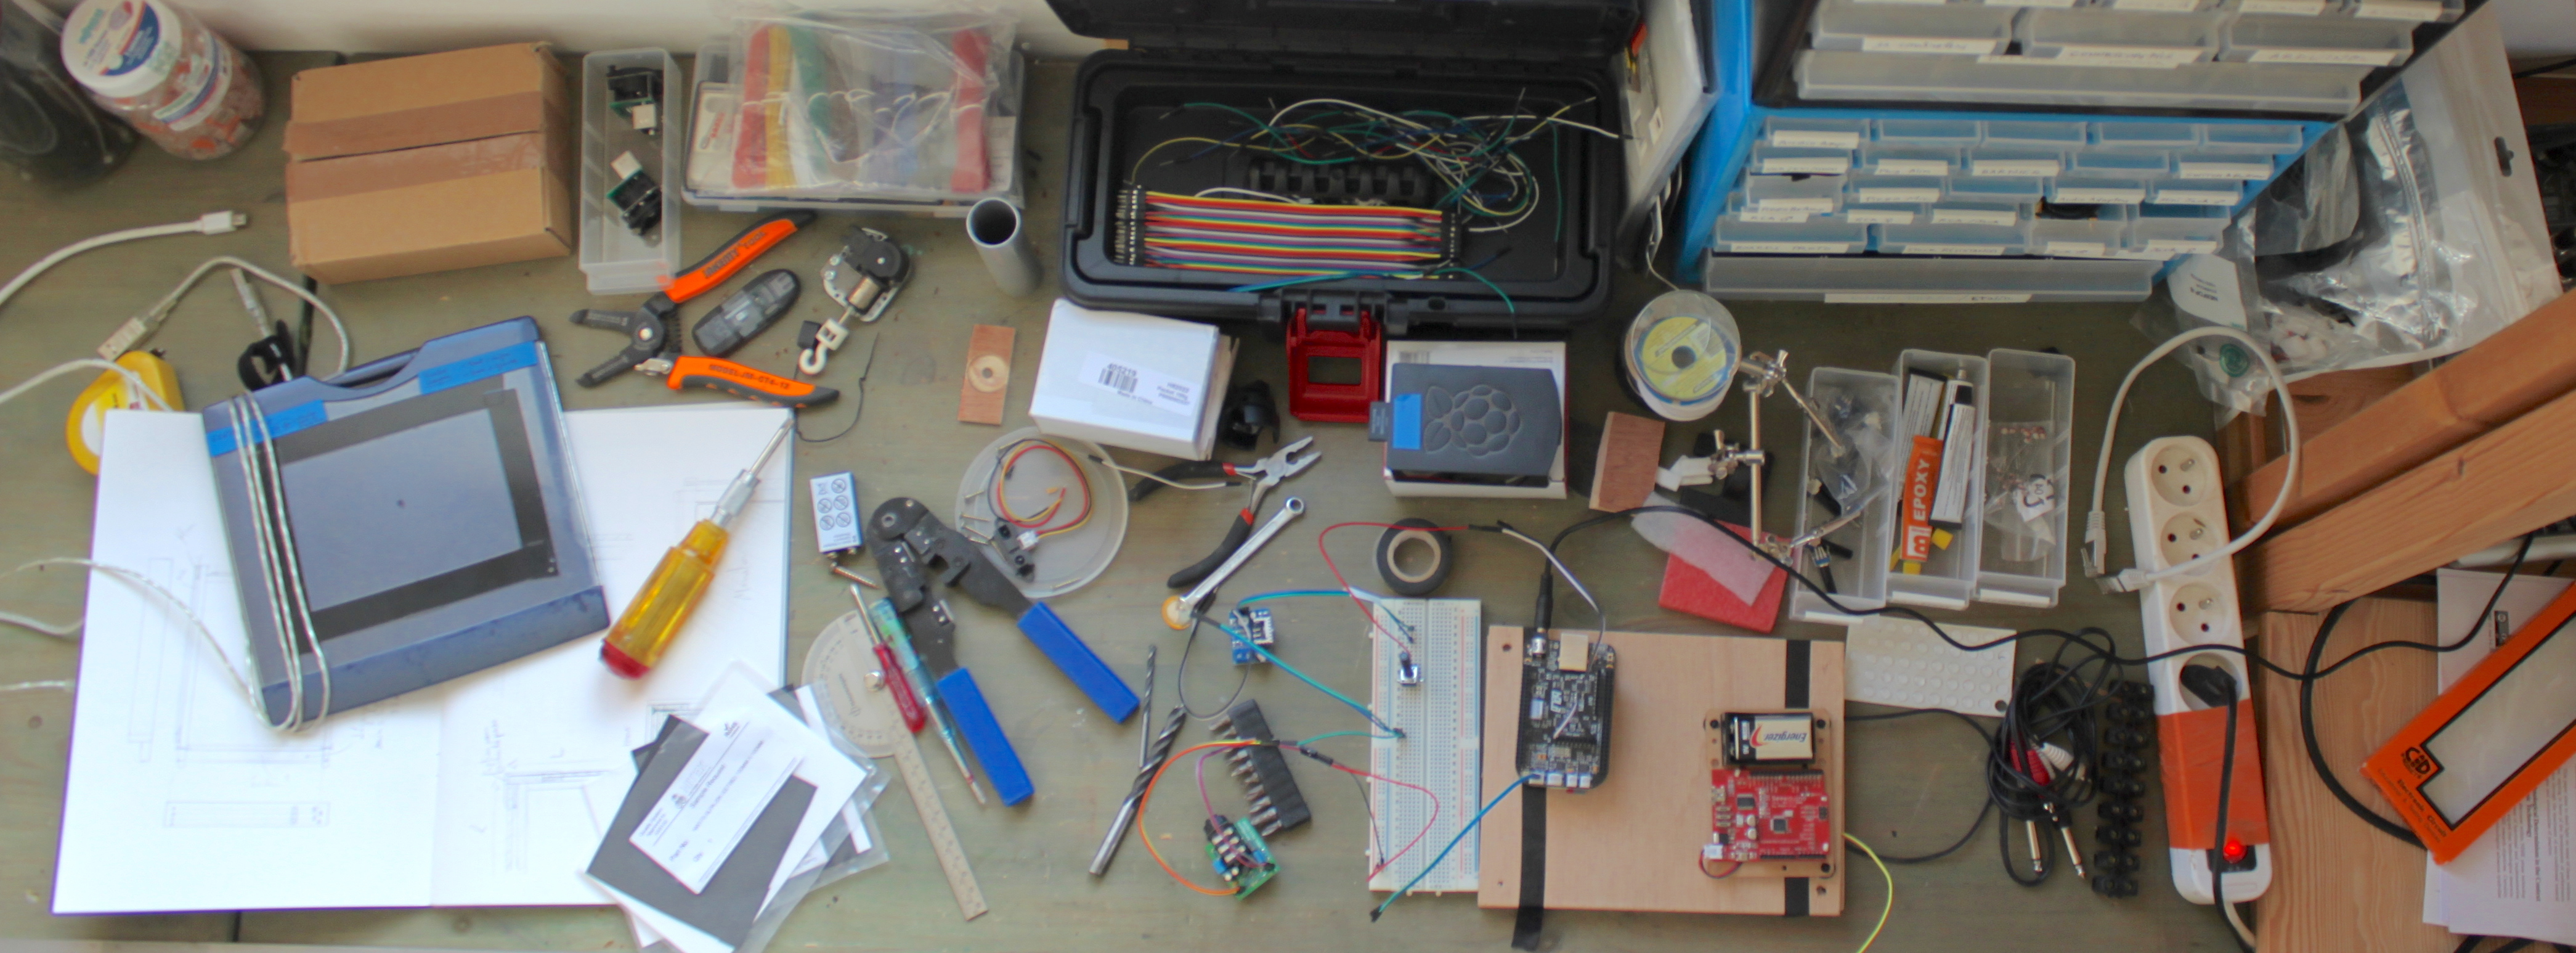
\includegraphics[width=\textwidth]{gfx/05_interfaces/lutherie-worktable.jpg}
	\caption[Matériaux sur la table d'un luthier numérique]{Matériaux sur la table d'un luthier numérique.}
	\label{fig:interface:table-luthier}
\end{figure}
%-------------------------- Figure : table du luthier numérique ----------------------------------

\noindent Une partie de la recherche sur les \gls{IHM} est motivée par la perspective d'une ``disparition de l'interface'' (\cite{weiser_computer_1991, dey_distributed_2001, hui_towards_2017}), au profit d'une \textit{informatique ubiquitaire} permettant une interaction directe avec les contenus plutôt qu'au moyen d'un support intermédiaire. Cette disparition de l'interface est liée --~parfois à tort, comme nous l'avons objecté dans le chapitre précédent~-- à l'idée de ``transparence'' de l'interaction, c'est à dire de correspondance entre l'attente d'un utilisateur et le résultat de son interaction avec la machine. Cette vision a été également appliqué au contexte de l'interaction musicale et, de façon relativement paradoxale, par des auteurs\footnote{On peut notamment citer Marc Leman :\iquote{What is needed is a transparent mediation technology that relates musical involvement directly to sound energy. Transparent technology should thereby give a feeling of non-mediation, a feeling that the mediation technology ``disappears'' when it is used. Such a technology would then act as a natural mediator for search-and-retrieval purposes as well as for interactive music-making.} \cite{leman_embodied_2008} ou encore Sydney Fels : \iquote{The more transparent the mapping is, the more expressive the device can be. The degree of mapping transparency for the player and audience form orthogonal axes of a graph into which devices can be placed. Full transparency for the player means that the device's output exactly matches the player's expectation and control.} \cite{fels_mapping_2002}.} fermement attachés à la notion d'\textit{embodiement}.\\
\indent Cependant, et paraphrasant la citation de Stravinsky en exergue de ce chapitre, les matériaux ne doivent pas être méprisés. Ils offrent de nombreuses possibilités, en terme de sensation, d'appui et de repos, et on peut s'en saisir aussi facilement que les délaisser--~quand il s'avère plus compliqué de délaisser un système immersif, voire ses propres pensées.\\
\indent Ce section regroupe une liste non-exhaustive de matériaux pouvant se retrouver sur la table de travail d'un luthier numérique. Ils sont regroupés en familles: matériaux bruts, capteurs, processeurs, mais l'agencement instrumental rend parfois leurs frontières poreuses (par exemple, un textile resistif et une plaque de métal peuvent servir à réaliser un capteur de pression). Cette liste dresse néanmoins un paysage général de ce répertoire, en en soulignant certains traits.

\subsection{Matériaux structurels}

\noindent Dans les instruments ``à contact'' (c'est-à-dire dans lesquels l'interaction passe par un rapport tactile avec l'interface de jeu), les matériaux structurels définissent l'agencement physique du \gls{DMI}: non seulement la distribution spatiale de son affordance mais également la cohésion et les liaisons mécaniques entre les différents capteurs. En effet, on touche rarement les capteurs de manière directe : ils sont recouverts, enveloppés, intégrés dans un objet matériel plus ou moins complexe, possédant son propre état de surface, son propre jeu mécanique, en liaison avec le reste du dispositif. Ils assurent la jonction autant que l'isolement entre les capteurs.
\vspace{-1em}
\begin{itemize}[noitemsep]
	\item \textbf{le bois}: Le contreplaqué est très souvent utilisé pour le prototypage rapide des \glspl{DMI} (cf. figure \ref{fig:interface:d-box}). Disponible en plaques de différentes épaisseurs, facilement découpable, perçable, collable et usinable par machine \gls{CNC}, il est un matériau très répandu dans la fabrication \gls{DIY} et les \glspl{makerspace}. Par ailleurs, le bois est historiquement le matériau phare de la lutherie acoustique. Il est par conséquent présent dans les instruments augmentés issus de lutheries acoustiques, mais son importance historique l'ancre de surcroît dans l'imaginaire collectif de l'instrument de musique. L'image d'Épinal de l'atelier du luthier est remplie de copeaux et de ciseaux à bois et, de même que le clavier, le bois contribue à donner un sentiment d'instrumentalité à un dispositif numérique. Ainsi, bien que n'ayant aucun rôle fonctionnel (excepté celui de sa sensualité), le bois massif est utilisé pour son caractère noble et évocateur sur certains instruments numériques high-tech, tels que le Linnstrument, le SoundPlane (cf. figure \ref{fig:interface:soundplane}), ou encore le Touché\footnote{\url{https://www.expressivee.com}};
	%------------------ Figure : D-Box and soundplane ---------------------
	% indenter avec https://tex.stackexchange.com/questions/54448/figure-with-caption-within-an-itemize-list-not-indenting-correctly ?
	\begin{figure}[!htbp]
		\makebox[\textwidth][c]{%
			\begin{subfigure}[b]{.4\textwidth}
				\centering
				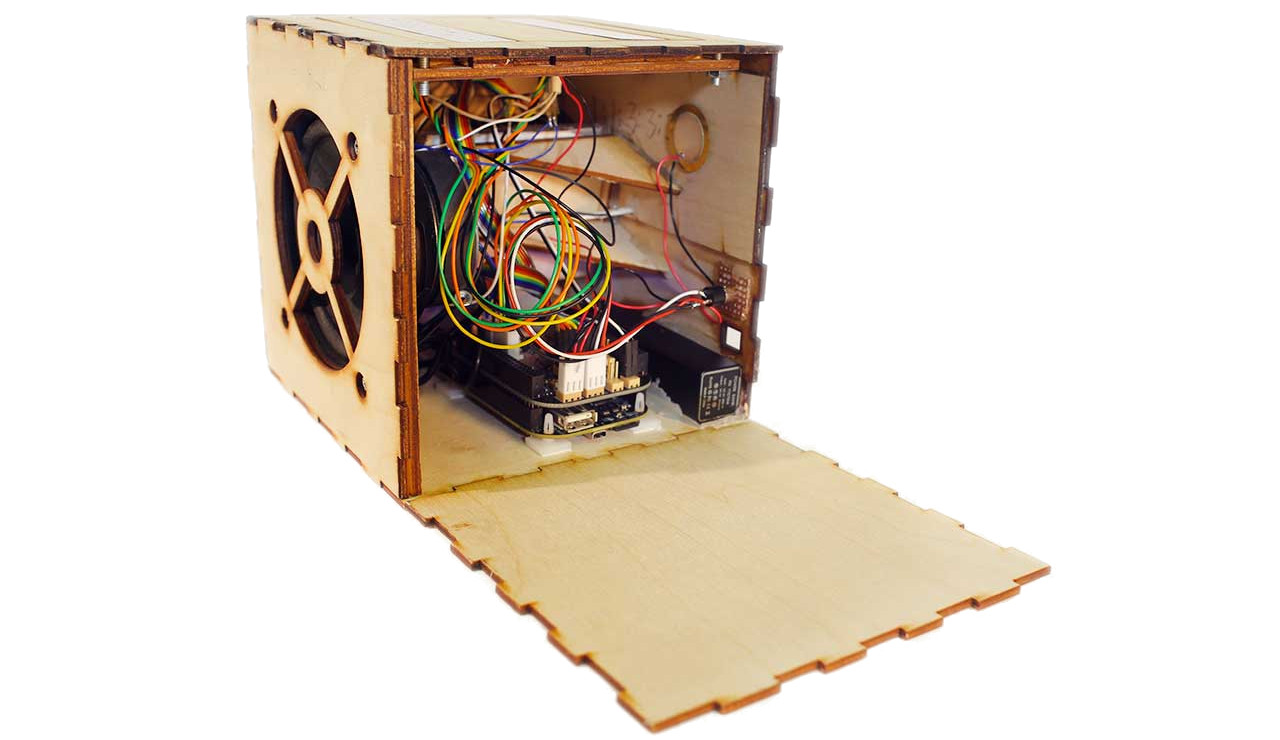
\includegraphics[width=\linewidth]{gfx/05_interfaces/d-box.jpg}
				\caption[La D-Box, un instrument ``hackable'']{La D-Box (cf. \cite{zappi_design_2014})}
			\label{fig:interface:d-box}
			\end{subfigure}%
			\begin{subfigure}[b]{.6\textwidth}
				\centering
		    	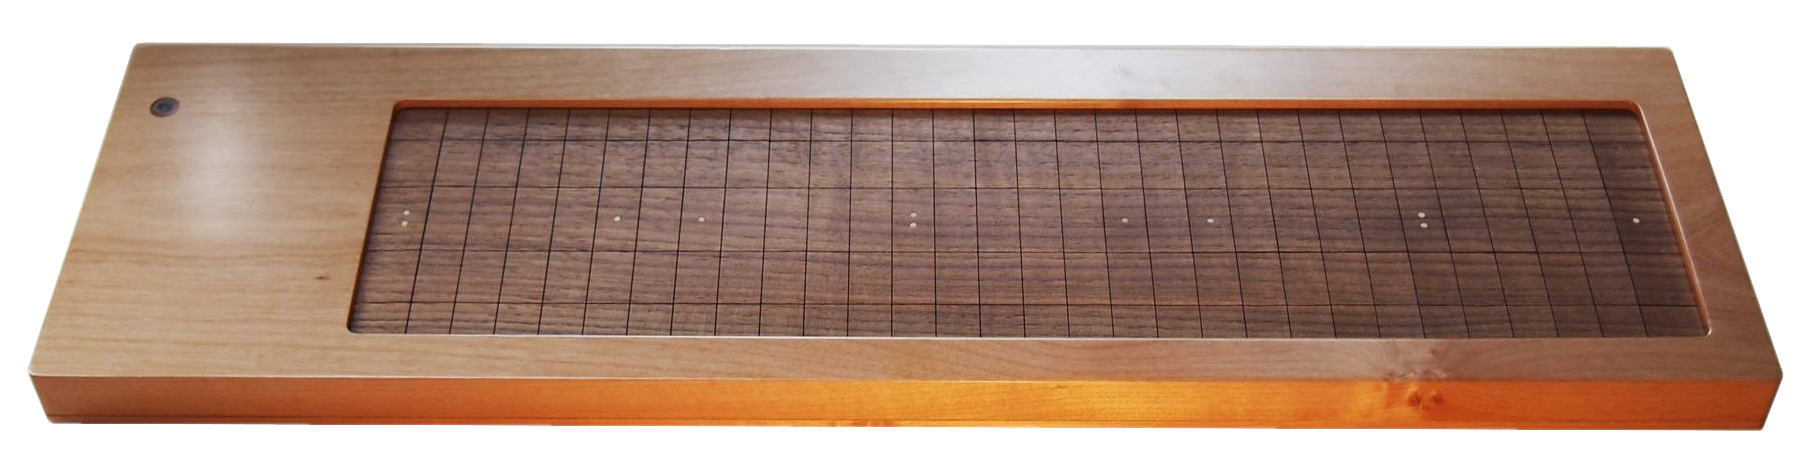
\includegraphics[width=\linewidth]{gfx/05_interfaces/soundplane.png}
				\caption[Le SoundPlane de Madrona Labs]{Le SoundPlane. © Madrona Labs}
				\label{fig:interface:soundplane}
			\end{subfigure}%
		}
		\caption{Contreplaqué ou massif : deux usages du bois dans les \glspl{DMI}.}
	\end{figure}
	%------------------ Figure : D-Box and soundplane ---------------------
	\item \textbf{le métal} est couramment utilisé pour les châssis et les coques de revêtement des machines électriques et électroniques. En dehors de ses propriétés de résistance mécanique, sa conductivité permet d'isoler les composants de faux contacts et de perturbations électromagnétiques et notamment d'éviter le ``bruit de masse'' qui peut survenir quand un équipement électrique tel qu'un \gls{DMI} n'est pas relié à la masse. Le métal possède également des propriétés de résonance acoustique qui en font un matériau intéressant pour la captation et la diffusion électro-acoustique, et utilisé par exemple dans le diffuseur ``Gong'' de l'onde Martenot;

	\item \textbf{le plastique} offre de grandes facilités de thermoformage, moulage, collage, perçage, gravage, qui permettent d'obtenir toutes sortes de formes et notamment de s'adapter à l'ergonomie du corps (e.g. la main du MI). Les propriétés de transparence du \gls{PMMA}\footnote{Aussi connu sous le nom commercial Plexiglass(®).} permettent de l'utiliser au-dessus d'un écran. L'essor des imprimantes 3D depuis le début du \siecle{21}~siècle a également contribué à son utilisation pour le prototypage rapide hors contexte industriel, dans les pratiques \gls{DIY} et les \glspl{makerspace};

	\item \textbf{la mousse} est généralement utilisée pour ses propriétés d'isolation phonique et vibratoire, mais également comme matériau tampon, pour augmenter la course des capteurs de pression (\gls{FSR}). Il existe de nombreuses sortes de mousses, offrant des nuances différentes d'enfoncement, de résiliance et affectant considérablement la sensation tactile sur ce type de capteurs;

	\item \textbf{le textile} a enfin été utilisé dans un certain nombre de \glspl{DMI} et de manière plus générale dans tout le champ d'interaction entre le domaine de la confection textile et de l'électronique, généralement désignée sous le terme de ``\textit{wearable electronics}''\footnote{Cf. la revue proposée dans \cite{stoppa_wearable_2014}}. La possibilité d'intégrer des fibres conductrices entrelacées dans le textile (``\textit{e-textile}'') a ainsi donné lieu à plusieurs développements de surfaces multitouch \cite{freed_application_2008, donneaud_designing_2017, wicaksono_fabrickeyboard:_2017} ou de vêtements munis de capteurs \cite{hayafuchi_musicglove_2008, serafin_controlling_2014, myllykoski_prototyping_2015};

	\item \textbf{le verre} est utilisé en particulier pour le caractère cristallin de sa résonance acoustique (e.g. Cristal Baschet, glass-harmonica). Une étude des cristallophones et de l'exploitation des qualités timbrales du verre dans les instruments électroniques a été proposée dans \cite{jensenius_evaluating_2010, frounberg_glass_2010}. Sa transparence permet d'offrir un support tangible à un écran où une caméra (voir par exemple \cite{savary_dirti_2012} ou la section \ref{sec:interfaces:phylogenese:xypre}). Plus difficile à travailler, son usage est toutefois moins courant dans les lutheries en général.
\end{itemize}

\subsubsection{Systèmes ``intermédiaires'' physiques}

\noindent Outre l'aspect structurel ``statique'', de nombreux systèmes mécaniques sont utilisés dans les \glspl{DMI}, venant modifier l'agencement spatial de l'instrument, ou transformer la relation avec les capteurs. Certains sont directement issus des lutheries traditionnelles; c'est le cas par exemple pour les touches de clavier, dont l'implémentation varie entre le simple contact direct sur un interrupteur bipolaire, et des systèmes plus complexes imitant la mécanique du clavier de piano (lestage des touches, mesure de la vitesse d'enfoncement, de pression et de relâchement la touche, etc...), d'autres sont d'origine extra-instrumentale, par exemple le système de pantographe développé par Ali Moméni pour contrôler un stylet de tablette graphique, présenté dans \cite{zbyszynski_ten_2007} ou le système d'articulation des bras sur le Méta-Instrument de Serge de Laubier). La notion de ``modèle intermédiaire'', transposée dans le domaine numérique, sera présentée plus en détail dans la section \ref{sec:algorithms:MID}.
% todo : mettre une figure pour illustrer les différents modèles de mécaniques de touches?

%%%%%%%%%%%%%%%%%%%%%%%%%%%%%%%%%%%%%%%%%%%%%%%%%%%%%%%%%

\subsection{Feed-in: capteurs}

\noindent Une grande diversité de capteurs est disponible sur le marché, mesurant différentes grandeurs physiques : position, distance, pression, orientation, flux d'air, son, lumière, humidité, température, champ magnétique, présence, contact, etc. Pour chaque grandeur mesure, la donnée sera encore variable selon les caractéristiques du capteur : sensibilité, résolution, précision, linéarité, bande passante, temps de réponse, etc. À cette diversité s'ajoute encore le fait que les capteurs intègrent de plus en plus souvent des algorithmes de traitement de signal, parfois programmables. Ces capteurs dits ``intelligents'' peuvent notamment réaliser des opérations de filtrage, mais également de la fusion de données permettant de renvoyer des informations de plus haut niveau\footnote{C'est le cas par exemple sur les capteurs dits \gls{AHRS}, sur les interfaces multitouch qui analysent une matrice de capteurs pour en extraire la position des points de contact}. Enfin, comme nous l'avons dit précédemment, les capteurs sont rarement utilisés de manière brute mais s'intègrent dans un agencement à la fois matériel, mécanique, électronique et algorithmique qui affecte leur réponse du tout au tout.\\
\indent L'utilisation spécifique de cette diversité de capteurs dans le domaine des lutheries numériques a été l'objet de nombreuses études qualitatives et quantitatives, menées en particulier depuis ces deux dernières décennies par l'équipe de Marcelo Wanderley à l'\gls{IDMIL}\footnote{Voir notamment : \cite{wanderley_choice_2000, hollinger_evaluation_2006, marshall_sensor_2009, vigliensoni_quantitative_2012, medeiros_comprehensive_2014} ainsi que le site \url{https://sensorwiki.org} qui rassemble un grand nombre d'informations techniques utiles sur les capteurs et les interfaces.}. En fournissant une analyse détaillée de leurs caractéristiques et en les intégrant dans des réalisations instrumentales fonctionnelles et jouées, ces études fournissent une base de données documentaire inestimable pour aider les luthiers numériques à ne pas se perdre dans cette multitude d'options possibles.\\
\indent Cependant, la généralisation de leur évaluation à des fins musicales reste délicate, en raison du fait que les instruments de musique constituent, comme nous l'avons déjà décrit dans les chapitres précédants, des \glspl{IHM} d'un genre particulier.

\subsubsection{Une analyse critique de la relation entre capteur et fonction musicale}

\noindent Un certain nombre d'études ont par ailleurs proposé une analyse de l'adéquation entre capteurs et fonctions musicale (e.g. \cite{vertegaal_towards_1996, goudeseune_interpolated_2002}), en mettant les aspects statique, dynamique, absolu ou relatif des valeurs transmises par les capteurs en regard de ces mêmes aspects appliqués à des valeurs musicales (en particulier la hauteur), dans l'optique d'évaluer qualitativement l'adéquation entre le choix des capteurs et le type de contrôle musical\footnote{Cette perspective reflète de manière plus générale une tendance de l'époque à vouloir répliquer le modèle instrumental classique ou la relation entre le geste et le résultat sonore est très directe. La remarque en conclusion de l'article d'Ungvary et Vertegaal \iquote{(...) a good causal mapping can ensure that tension is properly translated to the audible result.} en est révélatrice. Voir également la position de Claude Cadoz en ce sens au chapitre \ref{ch:gesture}.}. Bien qu'instructives et utiles dans la perspective d'une relation de mimétisme\footnote{Et les relations de mimétisme jouent un rôle essentiel dans les lutheries numériques, comme l'analyse Thor Magnusson dans \cite{magnusson_ergomimesis_2018}} univoque entre le mouvement gestuel et le mouvement d'un paramètre sonore, ces études mettent cependant de côté un aspect essentiel des \glspl{DMI}, à savoir la possibilité sans pareil des ordinateurs à traiter le signal et changer son échelle, transformer le continu en discret, l'absolu en relatif, l'instantané en différé, le statique en dynamique, et inversement, et plus encore.\\
%-------------------------- Figure : Vertegaal-transducer-function ----------------------------------
\begin{figure}[!htbp]
	\captionsetup{format=plain}%
	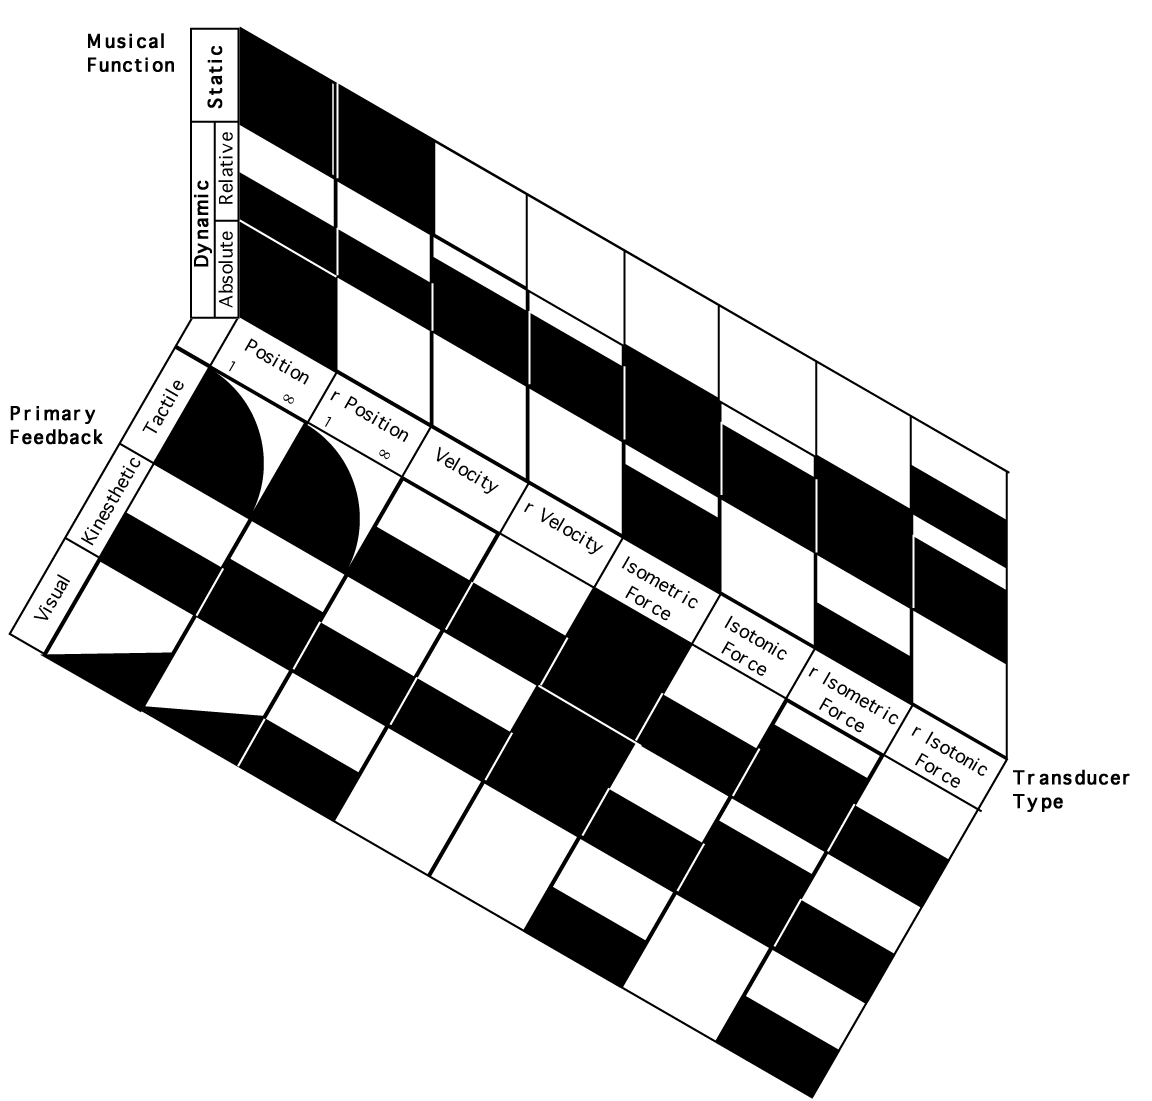
\includegraphics[width=\textwidth]{gfx/05_interfaces/vertegaal-musical-function.png}
	\caption[Adéquation entre fonction musicale, transducteur et retour primaire]{Adéquation entre fonction musicale, transducteur et retour primaire, selon \cite{vertegaal_towards_1996}.}
	\label{fig:interface:vertegaal-transducer-function}
\end{figure}
%-------------------------- Figure : Vertegaal-transducer-function ----------------------------------
\indent Ainsi d'après l'étude de Vertegaal (cf. figure \ref{fig:interface:vertegaal-transducer-function}), un potentiomètre linéaire serait très adapté à la sélection d'une valeur absolue de hauteur, tandis qu'un capteur de pression isotonique tel qu'un \gls{FSR} serait plus adapté à sa modulation. La validité de ce modèle ``subjectif'' (selon les termes des auteurs\footnote{Cf. \cite{ungvary_cognition_1999}}) a été confirmée expérimentalement par une étude récente\footnote{Cf. \cite{malloch_design_2019}}, mais dans un contexte de laboratoire et non un contexte musical réel. Il est ici intéressant de remarquer qu'un clavier de synthétiseur implémente quasiment l'exact opposé de la recommandation sus-mentionnée, en permettant de sélectionner des hauteurs absolues par un ensemble de capteurs de pression et de vélocité sous les touches, tandis qu'un potentiomètre rotatif --~mais présenté latéralement, ce qui rend sa course longitudinale plutôt que radiale~--, le ``\textit{pitch-bend wheel}'' permet leur modulation relative. La différence par rapport au modèle thérorique d'Ungvary et Vertegaal tient au fait que le mapping n'y est pas \textit{one-to-one} en ce qui concerne la hauteur, que le potentiomètre du \textit{pitch-bend-wheel} est muni d'un ressort de rappel et que ces deux capteurs contrôlent la hauteur de manière conjointe.\\
%-------------------------- Figure : table du luthier numérique ----------------------------------
\begin{figure}[!htbp]
	\captionsetup{format=plain}%
	\includegraphics[width=\textwidth]{gfx/05_interfaces/clavier-Martenot-MIDI.png}
	\caption[Agencement des capteurs et fonction musicale]{Un exemple de l'influence de l'agencement des capteurs sur leur usage musical: à gauche l'Onde Martenet: slider linéaire pour le contrôle de hauteur (avec la bague) et capteur de pression pour la modulation (d'intensité). À droite, un clavier MIDI : multiples capteurs de pression pour la sélection de la hauteur absolue et potentiomètre pseudo-linéaire pour la modulation (pitch-bend). Photographie de l'Onde Martenot : Wikipedia User:30rKs56MaE}
	\label{fig:interface:martenot-clavier}
\end{figure}
%-------------------------- Figure : table du luthier numérique ----------------------------------
\indent On voit donc que l'usage, la taille, l'agencement des capteurs et le traitement de ses données contribuent pour autant, sinon davantage, à définir les relations entre capteurs et paramètres musicaux, que la nature de la variation du capteur lui-même. Le fait qu'un paramètre musical ne soit pas ``facilement'' modulable avec un certain type de capteur ne présage donc pas de l'inadéquation de ce capteur pour le contrôle du paramètre en question. Tout au contraire, cela peut faire partie de la \textit{raison d'être} de l'instrument, dont la pratique s'apparente parfois davantage à celle du domptage d'un animal sauvage que celle de l'utilisation d'une machine docile\footnote{On pense par exemple au Theremin, sur lequel le contrôle de la hauteur par la distance de la main à l'antenne est très instable et difficile, et dont la maîtrise est probablement un des intérêt de sa pratique.}.

\subsection{Ordinateurs et DSP}
\label{sec:interfaces:computers_and_dsp}

\noindent Si les algorithmes d'un \gls{DMI} sont virtuels, les ordinateurs qui les font tourner sont bien réels et physiques. La principale remarque que l'on puisse faire à leur sujet, concernant leur aspect matériel, est la prodigieuse chute de leur coût et de leurs dimensions, depuis leur invention. Une conséquence directe de leur prix abordable a été leur démocratisation, et la conséquence de leur miniaturisation, leur intégration progressive dans des objets mobiles\footnote{Le smartphone en est un exemple significatif, qui a notamment permis le développement d'instruments autonomes tournant sur smartphone; voir par exemple le projet SmartFaust et la pièce ``\textit{Virtual rhizome}'' pour smartphones de Vincent Carinola: \url{https://youtu.be/cGZB44KI9Y0}\index[people]{carinola@Carinola, Vincent!virtualrhizome@\textit{Virtual Rhizome}}}. On peut distinguer dans cette évolution, cinq périodes d'une quinzaine d'années chacune, résumées dans le tableau \ref{table:computer-size}, la dernière en date étant couramment désignée comme celle de ``l'Internet des Objets'' (IoT, \textit{Internet of Things}).\\
\indent Si l'audionumérique temps-réel a depuis son origine été incarné par des dispositifs dans lesquels l'ordinateur, trop volumineux et lourd, était séparé de l'interface, cette dernière évolution est tout particulièrement intéressante en ce qui concerne les \glspl{DMI}. Elle augure la possibilité pour un public élargi de créer ses propres \glspl{DMI} intégrant interface de jeu et partie computationnelle dans un seul et même objet portable et (re)programmable. Des cartes électroniques comme \textit{Bela} ou \textit{The Owl}\footnote{Bela: \url{https://bela.io}; The Owl: \url{https://www.rebeltech.org}} et des langages comme \gls{FAUST} développé par le \gls{GRAME} \cite{orlarey_faust_2008} ou SOUL annoncé par Roli\footnote{Announced at the Audio Developer Conference 2018. \url{https://youtu.be/-GhleKNaPdk}} reflètent cette tendance.

\begin{table}[!htbp]
	\renewcommand{\arraystretch}{1.1}
	\captionsetup{format=plain}%
	\centering
 	\begin{tabularx}{\linewidth}{
 	>{\hsize=.9\hsize}X% 10% of 4\hsize 
 	>{\hsize=.6\hsize}X% 30% of 4\hsize
 	>{\hsize=.6\hsize}X% 30% of 4\hsize 
 	>{\hsize=1.4\hsize}X% 30% of 4\hsize
 	>{\hsize=1.5\hsize}X% 30% of 4\hsize
       % sum=4.0\hsize for 4 columns
       }
    \hkrule{1.2pt}
	\textbf{Période} &  \textbf{Nom} & \textbf{Taille} 	&  \textbf{Public} 	& \textbf{Audio}	\\
	\hline
	1950~--~1965 	& macro-	& salle		& laboratoires 		& non temps-réel 			\\
	1965~--~1980	& mini-  	& meuble 	& entreprises  		& contrôle temps-réel 		\\
	1980~--~1995	& micro- 	& caisse 	& foyers 			& temps-réel sur \gls{DSP} 	\\
	1995~--~2010 	& laptop 	& livre 	& individus			& temps-réel sur PC 		\\
	2010~--			& nano- 	& < main 	& plusieurs/individu	& temps-réel sur mobile 	\\
    \hkrule{1.2pt}\\[-10pt]
  \end{tabularx}
	\caption[Évolution de l'ordinateur : taille, accessibilité et capacités audio]{Évolution de l'ordinateur  : taille, accessibilité et capacités de calcul audio.}
	\label{table:computer-size}
\end{table}



\subsection{Feed-back: actionneurs}


\noindent En ``sortie'' de la machine, à l'autre extrémité de la boucle instrumentale --~si l'on peut dire~-- se trouvent les systèmes qui font le travail inverse des capteurs en venant \textit{agir} sur l'espace sensible. Là encore, de nombreux types d'actionneurs existent pour agir sur diverses dimensions, quoique celles qui nous intéressent plus directement dans le contexte musical soient celles du son, du mouvement et de la lumière (dans la mesure où l'expérience musicale est aussi une expérience \textit{gestuelle}\footnote{Cf. la notion de ``perception gestuelle'' qui recouvre le toucher et les différents aspects proprioceptifs dans \cite{cadoz_synthese_1981}} et visuelle du mouvement).\\
\indent D'un point de vue matériel, l'actionneur se présente comme un composant électronique connectable à l'ordinateur, généralement au moyen d'un \gls{CAN} et d'un amplificateur (parfois intégrés), qui adaptent le signal numérique au courant et voltage adaptés au transducteur. Le transducteur convertit ce signal électrique en oscillations acoustiques, en mouvements mécaniques, en intensités lumineuses, en champs électro-magnétique, etc.\\
\indent L'actionneur n'est toutefois jamais utilisé ``nu'' (sinon dans un modèle théorique erroné) mais toujours couplé à un support matériel qui filtre, amplifie, oriente la diffusion des mouvements de l'actionneur pour les rendre perceptibles. Par exemple, un haut-parleur est inséré dans une enceinte qui oriente la diffusion du son vers l'avant de l'enceinte; ou encore, un écran de vidéoprojection reçoit la trace lumineuse émise par un vidéoprojecteur.\\
\indent Les caractéristiques du matériau auquel l'actionneur est couplé peuvent ainsi considérablement influer sur le résultat sensible de l'action du capteur. Ainsi, un casque audio traduit le signal numérique en une vibration acoustique de manière relativement ``plate''\footnote{C'est à dire sans distordre le signal, ni en fréquence, ni en amplitude, ni dans le temps.} et directe à l'oreille, alors que ce même signal audio-numérique envoyé dans la corde d'une guitare via un transducteur tactile laissera entendre la résonance de la corde, de la caisse de guitare et du lieu (si par exemple on se trouve dans une salle de concert, plutôt que dans une chambre anéchoïque). De même, les rayons lumineux émis par un vidéoprojecteur pourront être envoyés sur des objets complexes (e.g. un bâtiment, ou de la fumée) qui transformeront la qualité du signal émis.\\
\indent La disposition spatiale des actionneurs joue également un rôle qu'il faut prendre en compte, car leurs actions peuvent selon les cas se complémenter (e.g. une image vidéo composée de plusieurs écrans juxtaposés, un front d'onde recréé par de multiples haut-parleurs dans la \gls{WFS}, etc.), interférer (e.g. l'opposition de phase qui créé des ``trous'' dans le spectre sonore quand des signaux harmoniques en phase synchrones sont envoyés sur plusieurs haut-parleurs) ou entrer en résonance (e.g. l'effet larsen résultant d'une boucle capteurs entre actionneurs se contrôlant et s'influençant mutuellement). La possibilité de pouvoir facilement assigner, sur ordinateur, des relations de correspondances entre n'importe quel type de capteur et n'importe quel type d'actionneur entraîne la possibilité de larsens multi-modaux : par exemple un système dans lequel le son est capté par un microphone, utilisé pour générer une image, l'image utilisée pour générer du son, capté par le microphone.)\\
\indent En dernier lieu, si l'on peut envisager une action directe des actionneurs sur notre perception, sans médiation intermédiaire\footnote{Ce qui est le cas dans des dispositifs tels que la projection rétinienne, les implants cochléaires ou neuronaux.}, il faut encore considérer les effets de notre perception, qui en plus de filtrer, d'amplifier, de focaliser elle aussi (comme un matériau) discrimine, ordonne, interprète, construit, aime ou rejette les signaux que nous recevons, en s'ajoutant à la médiation complexe qui opère entre la représentation numérique du signal sur l'ordinateur et la perception du phénomène sensible provoqué par les actionneurs.\\
\indent Outre les caractéristiques techniques de l'actionneur (puissance, bande passante, course, etc.), il faut donc ainsi prendre en compte les propriétés des matériaux auquel les actionneurs sont couplés, en y incluant les processus cognitifs à l'œuvre dans la perception de leur action sur le sensible\footnote{L'étude des propriétés acoustiques des matériaux ainsi que des mécanismes de la psychologie cognitive mène par ailleurs à l'élaboration de modèles utilisables dans les lutheries numériques. Cf. section \ref{sec:algorithms:MID}.}. À défaut, s'intéresser à ces caractéristiques prises isolément risque de conduire à oublier leur articulation dans l'instrument lui-même, comme le note François Dumeaux : \iquote{Quand tu composes par exemple une pièce, combien de fois je me suis retrouvé à aligner des belles courbes ... c'était pas avec les oreilles que je faisais ma courbe de volume, c'était avec mes yeux. Voilà, (...) tu te retrouves à faire des trucs absurdes, à être tatillon... [à dire, en parlant des valeurs MIDI de la courbe] ``ah non c'était à 127!'',  alors qu'en fait on n'entend pas la différence...} (entretien personnel, cf. annexe \ref{appendix:dumeaux}).

%%%%%%%%%%%%%%%%%%%%%%%%%%%%%%%%%%%%%%%%%%%%%%%%%%%%%%
\section{La part acoustique de l'interface des DMIs}
\label{sec:interfaces:part_acoustique}

\noindent Il faut ici rappeler que les \glspl{DMI}, s'ils se caractérisent par l'usage de la computation numérique, sont aussi nécessairement des instruments électroniques, électriques et acoustiques. Il portent l'héritage et les contraintes propres à ces différents médias. Mais le phénomène acoustique, omnidirectionnel et tri-dimensionnel dans le monde physique, est réduit dans l'électronique numérique à un signal mono-dimensionnel\footnote{Nicolas Collins, dressant une liste de traits distinctifs entre hardware et software dans \cite{collins_semiconducting_2013} notait: ``Traditional acoustic instruments are three-dimensional objects, radiating sound in every direction, filling the volume of architectural space like syrup spreading over a waffle. Electronic circuits are much flatter, essentially two-dimensional. Software is inherently linear, every program is a one-dimensional string of code.''} et mono-directionnel\footnote{Au niveau logiciel, des blocs bi-directionnels de plus haut niveau peuvent cependant être crées, comme par exemple dans la librairie de modèles physiques pour \gls{FAUST}, cf. \cite{berdahl_introduction_2012} et \cite{michon_faust_2018}.}, introduisant une distinction entre les ``entrées'' d'une part et les ``sorties'' d'autre part. La dimension acoustique des \glspl{DMI} s'intègre donc dans un circuit ouvert ou fermé avec le système de computation via des transducteurs acoustiques --~microphones en entrée, ou haut-parleurs en sortie.\\
% \indent Par ailleurs, la vibration acoustique peut-être ressentie de manière auditive, quand sa transmission est aérienne, ou tactile lorsqu'elle est solidienne. Ces deux types de vibrations correspondent généralement à deux technologies de transducteurs différentes.

\subsection{Captation : microphones et transducteurs piezo}

\noindent La captation en direct de son acoustique dans un instrument électronique est une pratique très courante chez les musiciens électroacoustiques, et permet des séquences de jeu en prise directe avec des sons concrets, amplifiés, enregistrés, transformés par l'instrument (ou non). En particulier, l'usage de microphones, notamment de transducteurs piezo dits ``microphones de contact'', vient redonner une composante acoustique au corps physique de l'agencement instrumental (et du musicien s'il utilise directement sa voix et son corps), cette composante acoustique ``naturelle'' étant sinon généralement couverte par la puissance du son amplifié. L'intérêt principal réside dans la richesse du signal capté, comme le note Miller Puckette\footnote{``(...) sliding a brush over a drum trigger isn’t likely to produce  anything  useful,  whereas  doing  the  same  thing on an instrument that operates directly on the audio signal from the contact microphone (as we do here) has the possibility to create a wide range of useful musical sounds.'' \cite{puckette_infuriating_2011}.} : \iquote{(...) il y a peu chance que le frottement de balais sur un pad de batterie produise quoi que ce soit d'intéressant, alors que faire la même chose sur un instrument qui fonctionne directement avec le signal audio du microphone de contact (...) offre la possibilité de créer une large gamme de sons musicaux utiles.} L'usage d'algorithmes d'analyse en temps-réel permet, au-delà d'effets déjà existants dans le domaine électroacoustique, d'utiliser les caractéristiques du son comme paramètre de contrôle\footnote{L'interface Mogees est par exemple principalement basée sur ce principe (\url{https://www.mogees.co.uk}), voir également l'Annexe \ref{appendix:zamborlin}.}. Plusieurs stratégies sont possibles, consistant à utiliser le signal comme source d'excitation de modèles physiques (\cite{momeni_composing_2005, schlessinger_kalichord_2009, mehes_virtual-acoustic_2017, williams_pitch_2017, robertson_harmonic_2018}), de filtrages convolutifs (\cite{schwarz_rich_2014}), ou encore d'utiliser des paramètres de plus haut niveau extraits du signal. En particulier, le suivi temps-réel de pitch, s'il reste un problème ouvert dans le domaine des \gls{MIR}, bénéficie d'une histoire de plus de 40 ans (\cite{noll_cepstrum_1967}) et de nombreux algorithmes relativement efficaces sont disponibles (\cite{boersma_accurate_1993, de_cheveigne_yin_2002,pardue_low-cost_2015, schramm_polyphonic_2018}). Le suivi de hauteur (ainsi que d'autres caractéristiques du son) a été particulièrement développé à l'\gls{IRCAM} et est utilisé en concert, depuis le développement d'Antescofo\footnote{\label{fn:interface:antescofo} Antescofo est la dernière version des systèmes de suivi de partition développés à l'\gls{IRCAM}. Au-delà du suivi, Antescofo intègre par ailleurs un système de programmation synchrone qui permet de synchroniser des événements (e.g. musicaux) avec des motifs repérés dans ce qui est capté par le système.}, dans de nombreuses pièces mixtes pour instruments acoustiques captées en temps-réel\footnote{Un exemple en est la pièce \textit{En Echo} de Philippe Manoury\index[people]{manoury@Manoury, Philippe!enecho@\textit{En Echo}}, une des premières pièces utilisant un suivi audio temps réel (sur la voix), ainsi que l'extraction des hauteurs des différents formants de la voix pour contrôler la synthèse.}.


\subsection{Diffusion : haut-parleurs et transducteurs tactiles}

\noindent Dans le cas le plus trivial, l'acoustique des \glspl{DMI} se limite à la membrane du haut-parleur qui transforme \textit{in fine} le signal audio-numérique en son acoustique\footnote{Le choix des haut-parleurs peut jouer un rôle primordial, comme c'est le cas dans la musique acousmatique diffusée sur orchestre de haut-parleur ou ``acousmonium''. Voir en particulier \cite{mooney_sound_2006}}. À la différence des instruments acoustiques, la diffusion et la projection du son est souvent séparée de l'interface gestuelle et, bien souvent, distante du musicien quand elle est ``spatialisée''. La spatialisation du son a en effet joué un rôle essentiel dans la motivation des concerts électroacoustiques ``live'', à une époque où l'arrivée du \gls{CD} est vendue comme la possibilité d'une écoute de salon ``haute-définition'' équivalente à l'expérience du concert\footnote{Comme en témoignent les publicités de l'époque, par exemple celle de Phillips mettant en scène un public les yeux bandés incapables de faire la différence entre le concert et l'écoute d'un \gls{CD}: \url{https://youtu.be/jtNyWmD3EQ4}}, comme le raconte Serge de Laubier en parlant des origines du PSO\footnote{``Processeur Spatial Octophonique'', système de spatialisation inventé par De Laubier en 1986.} et du Méta-Instrument dans les années 1980 : \iquote{Si on entend mieux chez soi, c'est pas la peine de faire des concerts, donc il faut qu'au concert, il y ait une expérience unique qui vaille le coup de se déplacer, d'où réfléchir à un système de spatialisation.} (communication personnelle, cf. annexe \ref{appendix:delaubier}).\\
\indent Mais le retour acoustique peut également être perçu dans sa dimension tactile. Ronald Verillo montre que la sensibilité du doigt est capable de perçevoir des vibrations jusqu'au kHz \cite{verillo_vibration_1991} et dans les années 1990 plusieurs \glspl{DMI} explorent les possibilités offertes par un retour vibrotactile dans l'interface de jeu \cite{chafe_tactile_1993, bongers_tactual_1998}. Au début des années 2000, plusieurs études propose une analyse de tels dispositifs à la fois sous l'angle technique et dans la perspective de leurs usages dans les \glspl{DMI} (e.g. \cite{rovan_typology_2000, marshall_vibrotactile_2006, birnbaum_towards_2005}). L'essor progressif des transducteurs tactiles à large bande audio depuis la dernière décennie a renouvelé l'intérêt pour le vibrotactile en permettant de l'associer directement au retour audible via le rayonnement acoustique d'un matériau support, comme c'est le cas dans les instruments augmentés à contrôle actif tels que la \textit{Smart Guitar} de HyVibe\footnote{\label{fn-hyvibe}\url{https://www.hyvibe.audio}}. Ce retour vibro-acoustique présente plusieurs intérêts :
\vspace{-1em}
\begin{itemize}[noitemsep]
	\item \textbf{offrir au musicien un retour vibratoire} (et/ou auditif), qui lui permet de mieux ressentir le résultat sonore et pouvoir plus facilement identifier sa contribution personnelle dans le cas de musique d'ensemble\footnote{Voir par exemple les systèmes \textit{SubPac} (\url{https://subpac.com}), ou \textit{Basslet} (\url{https://lofelt.com}) commercialisés pour augmenter la perception du son par la vibration tactile.};
	\item \textbf{faciliter l'identification et la localisation} auditive des instruments et accroître la lisibilité des relations geste/son pour le public;
	\item \textbf{bénéficier des propriétés acoustiques des matériaux} structurels de l'instrument, notamment leur rayonnement, beaucoup plus singulier que celui des haut-parleurs (dont la conception est généralement orientée vers un rayonnement homogène et une bande-passante plate);
	\item \textbf{introduire du feedback} dans le corps de l'instrument en recaptant cette vibration. Traité avec une latence suffisamment faible, le \textit{feedback} laisse la possibilité de transformer dynamiquement les propriétés acoustiques des matériaux, comme le fait par exemple le système HyVibe\footref{fn-hyvibe};
	\item \textbf{communiquer des informations} à l'instrumentiste via un retour vibratoire, tel que le frettage virtuel\footnote{cf. infra, section \ref{sec:audio-fretting}}, ou des informations sémiotiques de plus haut-niveau\footnote{Voir en particulier le travail de Gabriela Patiño-Lakatos et al. \cite{patino-lakatos_paradigmes_2019} sur la communication intersubjective d'information par voie vibrotactile.}.
\end{itemize}

\subsection{Boucler la boucle}

\indent Paradoxalement, si le résultat acoustique d'un instrument est \textit{in fine} ce qui nous intéresse le plus, la part acoustique de l'instrument numérique est aussi la plus problématique. Sur un instrument acoustique, le contrôle du son se fait directement, de manière haptique. Il est ainsi possible d'exciter un élément résonant (e.g. une corde ou une peau) et d'étouffer sa résonance en appliquant simplement la main sur les éléments résonants. La surface du résonateur, qui présentent un nombre infini de modes de résonance, permet de plus d'interagir directement avec tous ces modes. Par exemple, on peut sélectionner des harmoniques sur une guitare en positionnant son doigt sur un nœud de vibration du mode en question, ou encore obtenir un timbre ``étouffé'', filtré de ses modes d'ordre élevé par une technique de \textit{palm-muting} sur l'extrémité des cordes d'une guitare. C'est une manière très intuitive d'agir avec le timbre d'un instrument de manière tangible.\\
\indent Dans le cas où le système microphone/DSP/haut-parleur est non-bouclé (typiquement, quand les haut-parleurs sont éloignés des microphones), on contrôle facilement le filtrage de la source, sans que posent de vrais problèmes de stabilité, ce qui permet d'appliquer toute sorte de transformations actives ou passives, linéaires ou non.\\
\indent Dans le cas où les haut-parleurs et microphones ne sont plus distants, mais intégrés à l'interface, les effets de feedback rendent les traitements beaucoup plus instables. La stabilité globale nécessite que le système électronique soit l'équivalent d'un système physique analogique\cite{berdahl_feedback_2012}, ce qui contraint fortement l'espace des transformations possibles et constitue un problème de traitement du signal ouvert\footnote{Voir notamment les travaux de l'équipe S3AM de l'\gls{IRCAM} sur ce sujet : \cite{muller_power-balanced_2018, falaize_passive_2018, muller_minimal_2019}}. La recherche dans le domaine du ``contrôle actif'' qui s'intéresse précisément aux possibilités de modification dynamique des propriétés acoustiques d'un matériau physique, a développé ces dernières décennies un ensemble de modèles \cite{boutin_active_2011, benacchio_mode_2015, meurisse_active_2015, pardue_separating_2019} et de techniques pour faire face à ce problème, sans l'avoir totalement résolu. Essentiellement, il s'agit de soustraire la contribution de l'actionneur au signal capté par le microphone d'une part en échantillonant à haute fréquence, de traiter le signal avec une latence la plus faible possible, et de n'utiliser que des filtres linéaires passifs pour éviter un repliement spectral qui pourrait faire diverger le signal.\\
\indent À défaut d'une solution idéale, l'utilisation de microphones et de transducteurs acoustiques dans le corps physique de l'instrument reste une option intéressante tant au niveau sonore qu'au niveau tactile, sans nécessairement nécessiter une stabilité absolue du système. On peut ici tirer partie du fait que les gains en entrée comme en sortie peuvent être ajustés dynamiquement (et donc, être ``joués'' comme d'autres paramètres), soit pour utiliser alternativement le microphone et le haut-parleur, soit pour jouer de leur instabilité conjointe. Dans ce dernier cas, l'usage de filtres et de compresseur (notamment) permet de garder l'amplitude et la fréquence du signal dans une zone non-douloureuse de l'audition, et même, une zone riche en qualité de timbre. C'est cette solution pratique qui a été utilisée dans le développement du Filigramophone et du Xypre.


%%%%%%%%%%%%%%%%%%%%%%%%%%%%%%%%%%%%%%%%%
\section{Ergonomie, ergodynamisme}
\label{sec:interfaces:ergonomy}

\subsection{Portabilité de l'interface}
\label{sec:interfaces:ergonomy:portability}

\noindent Avant d'évoquer l'ergonomie de l'instrument en situation de jeu, notons ici que l'instrument (et l'instrumentiste) a une vie en dehors de son usage musical sur scène. Le musicien est amené à [faire] transporter son instrument, à pied, en métro, en voiture, en camion, en avion... Le hardware, comme son nom l'indique, est ``dur'', concret, matériel. Son poids et ses dimensions affectent sa transportabilité et constituent un facteur contraignant pour le musicien. Sa dématérialisation dans des alternative logicielles —\textit{soft}, plus douces et légères— permet d'intégrer dans les limites acceptables pour leur transport, certaines fonctionnalités offertes par les équipements \textit{hard}. En particulier, la virtualisation des outils d'ingénierie du son (table de mixage, équaliseurs, compresseurs et autres effets) permet leur intégration dans l'instrument lui-même\footnote{Ainsi, Serge de Laubier qui utilisait jusqu'en 2005 une table de mixage Yamaha O2R (31kg) motorisée et contrôlée directement depuis son Méta-Instrument, ainsi qu'un échantilloneur EMU (4,5kg) a progressivement conçu des émulations logicielles tournant sur un MacBookPro (1.8kg) de ces équipements pour alléger le transport. Pour une analyse approfondie de cette importance critique du poids des \glspl{DMI}, voir l'analyse de John Richards dans \cite{richards_32kg_2006}. Par ailleurs, les émulations logicielles permettent de réaliser d'autres fonctions qui n'étaient pas présentes dans les modèles originaux. De même, voir les propos d'Adrien Mamou-Mani (annexe \ref{appendix:mamou-mani}) sur l'intérêt que trouvent les ingénieurs du son à ce qu'une partie du traitement audio soit pris en charge par l'instrument lui-même}. Cela étant, la part scénographique des instruments fait que leurs dimensions peuvent également être impratiques à dessein\footnote{Le but d'un instrument n'est pas de nous simplifier la vie, alors que l'absence d'effort constitue \iquote{une vertu cardinale dans la mythologie de l'ordinateur} comme le notait Joel Ryan dans \cite{ryan_remarks_1991}.} pour confronter le musicien et le public à un objet hors-norme\footnote{Cf. par exemple le projet ``Machine \_ Variation'' de Nicolas Bernier\index[people]{bernier@Bernier, Nicolas!machinevariation@\textit{Machine \_ Variation}} et Martin Messier\index[people]{messier@Messier, Martin!machinevariation@\textit{Machine \_ Variation}}, et les observations de Bernier en annexe \ref{appendix:bernier}.}.\\
\indent Les instruments peuvent prendre différentes formes, plus ou moins grandes, qui définissent à la fois leur portabilité ainsi que la posture du musicien envers son instrument. On peut distinguer quatre types de rapport à l'interfaces de jeu impliquant différent rapports de proximité avec l'instrument:
\vspace{-1em}
\begin{itemize}[noitemsep]
	\item \textbf{interfaces portable}, qui \textit{adhèrent} au corps. L'interface est \textit{portée} (comme un habit) et les mouvements du corps sont captés directement et en permanence, par exemples sont le Méta-Instrument 3, The Hands, le Myo d'Atau Tanaka, la guitare électrique, etc.;
	\item \textbf{interfaces portative}, qu'on peut \textit{prendre} et \textit{tenir} dans ses mains pour en jouer, mais également \textit{poser} (comme un ustensile), par exemple ``The Sponge'' de Martin Marier\index[people]{marier@Marier, Martin}, un tambourin, un gamepad, un harmonica;
	\item \textbf{interfaces statue}\footnote{Claude Cadoz nomme ce type de configuration ``dispositif à vis-à-vis'' dans \cite{cadoz_geste_1994}}: objets trop grands pour être déplacés (où qui n'a pas vocation à) mais autour duquel on peut tourner. L'instrument est \textit{touché} (comme une sculpture), par exemple les claviers, et pad \gls{MIDI}, les ``intonarumori'' de Bernier/Messier\index[people]{messier@Messier, Martin!chambredesmachines@\textit{La chambre des machines}}\index[people]{bernier@Bernier, Nicolas!chambredesmachines@\textit{La chambre des machines}}\footnote{Voir \url{http://www.lachambredesmachines.com}}, les synthétiseurs modulaires en rack, le Théremin, etc.);
	\item \textbf{interfaces immersives} : captant une variation particulière dans l'intégralité de l'environnement. L'instrument est \textit{enveloppant} (comme un lieu), et joué en étant \textit{parcouru}. Il m'entoure mais je n'ai pas directement accès à lui, par exemple les instruments basés sur caméra ou Kinect, les installations sonores utilisant la réalité virtuelle (CAVEs, etc.).
\end{itemize}
\clearpage
\begin{wrapfigure}[12]{r}{0.44\textwidth}
	\vspace{-1em}
	\captionsetup{format=plain}
	\centering
 	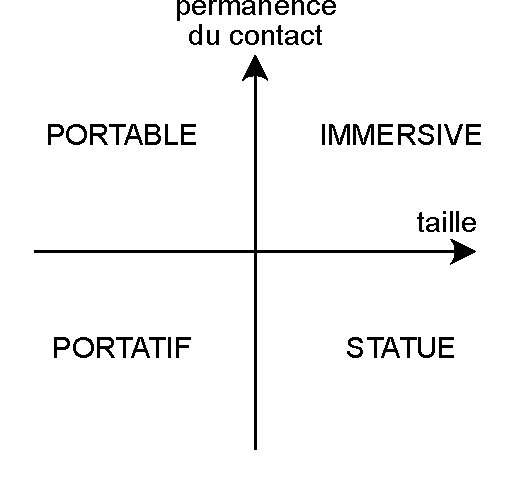
\includegraphics[width=0.4\textwidth]{gfx/05_interfaces/interface-portabilite.pdf}
 	%\vspace{-2em}
	\caption[Portabilité et permanence du contact avec l'interface.]{Portabilité et permanence du contact avec l'interface.}
 	\label{fig:interfaces:portabilite}
\end{wrapfigure}
\par
\noindent Ces catégories ne sont pas étanches; par exemple, un synthétiseur à clavier se jouera aussi bien assis, que debout, que porté en bandoulière dans le cas des \textit{Keytars}\footnote{contraction des termes \textit{keyboard} et \textit{guitar} désignant les synthétiseurs à clavier qui se portent comme les guitares électriques.}. On représenterait mieux ces catégories par un espace continu, polarisé par la taille de l'interface en abscisse et la permanence du contact \underline{requis par l'instrument} en ordonnée (figure \ref{fig:interfaces:portabilite}). L'origine des abscisse serait alors un rapport de taille à la limite de ce qu'il est possible de porter, et qui constitue un point de clivage en terme d'usage. L'ordonnée s'étend entre deux extrêmes représentant un contact permanent (tel que dans une installation immersive) et un contact inexistant, ou du moins limité à son activation (instrument autonome).
%-------------------------- Figure : wacom ---------
% \begin{figure}[!htbp]
% 	\captionsetup{format=plain}%
% 	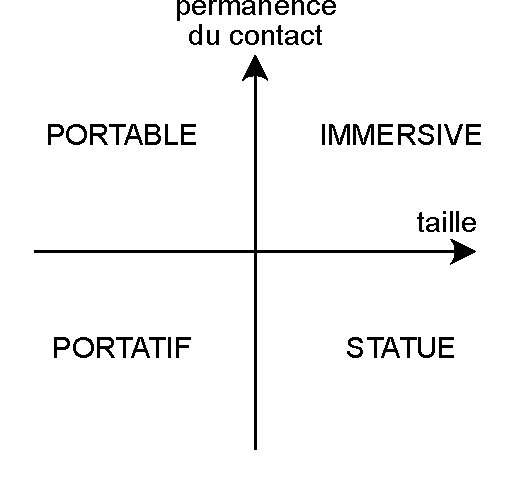
\includegraphics[width=\textwidth]{gfx/05_interfaces/interface-portabilite.pdf}
% 	\caption[Portabilité et permanence du contact avec l'interface.]{Portabilité et permanence du contact avec l'interface.}
% 	\label{fig:interfaces:portabilite}
% \end{figure}


% \setlength\intextsep{12pt}
% \begin{wrapfigure}[16]{r}{0in}
%   ...
% \end{wrapfigure}
% \vspace{-15pt} \leavevmode\section{Section title}
%-------------------------- Figure : wacom ---------


% \begin{table}[!htbp]
% 	\renewcommand{\arraystretch}{1.1}
% 	\captionsetup{format=plain}%
% 	\centering
%  	\begin{tabularx}{\linewidth}{
%  	>{\hsize=1\hsize}X% 10% of 4\hsize 
%  	>{\hsize=1\hsize}X% 30% of 4\hsize
%  	>{\hsize=1\hsize}X% 30% of 4\hsize 
%        % sum=4.0\hsize for 4 columns
%        }
%     \hkrule{1.2pt}
% 	\diagbox{mobilité}{contact}	&  \textbf{permanent} & \textbf{temporaire} \\
% 	\hline
% 	\textbf{immobile} 					& immersif					& sur pied					\\
% 	\textbf{mobile} 							& vêtement  				& outil 			\\
%     \hkrule{1.2pt}\\[-10pt]
%   \end{tabularx}
% 	\caption[Portabilité et contact]{Portabilité et contact.}
% 	\label{table:portabilite}
% \end{table}



\subsection{Disponibilité de l'interface}
\label{sec:interfaces:ergonomy:disponibility}

\noindent L'agencement modulaire des \glspl{DMI} entraîne par ailleurs un temps de démontage-remontage de l'instrument avant qu'il soit possible d'en jouer. Leur fonctionnement nécessite généralement la disponibilité de prises de courant à proximité, voire de réseau WiFi. Il faut ensuite câbler les haut-parleurs distants (pour la spatialisation du son), les capteurs et/ou actionneurs parfois distants eux-aussi (e.g. lors de l'usage de caméra), les machines qui fonctionnent en réseau, et les divers modules (carte son, interface d'acquisition, microphones, boites de direct, etc.) Se rajoute ensuite le ``temps de lancement'', c'est-à-dire le temps de démarrer l'ordinateur, de lancer le(s) logiciel(s) nécessaire(s), d'ouvrir le patch ou le script adéquat, et éventuellement de l'initialiser avec la bonne configuration. S'ajoute enfin le temps préalablement passé (même si les surprises au moment du concert peuvent arriver) à maintenir la partie algorithmique opérationnelle avec les changements d'\glslink{OS}{OS} et les mises à jour logicielles, comme il a été souligné dans le chapitre \ref{ch:ephemeral} et dans l'étude de Morreale et McPherson \cite{morreale_design_2017}.\\
\indent Le terme ``plug'n play'' est couramment utilisé pour qualifier une disponibilité immédiate de l'instrument, mais sur de tels dispositifs, la temps de branchement peut dans les faits s'avérer assez long. Il est important de prendre en compte cette durée dans le design d'un \gls{DMI}, car tout le temps passé sur la partie de montage technique est pris au détriment du temps de jeu\footnote{Cf. les propos de Nicolas Bernier\index[people]{bernier@Bernier, Nicolas} (annexe \ref{appendix:bernier}), François Dumeaux\index[people]{dumeaux@Dumeaux, François} (annexe \ref{appendix:dumeaux}) et Bruno Zamborlin (annexe \ref{appendix:zamborlin}) dans les entretiens.}. Notons toutefois qu'à la différence des instruments acoustiques, les \glspl{DMI} ne nécessitent généralement pas de temps d'accordage et ne sont généralement pas sujets aux conditions de température et d'hygrométrie requérant un ré-accordage et un ``temps de chauffe'', particulièrement pour les cuivres.


%------------------------------------------------------------
\subsection{Se repérer dans l'interface}
\label{sec:interfaces:ergonomy:cues}

\noindent L'apprentissage et la maîtrise d'un instrument passe par une exploration multimodale qui implique l'ensemble de la perception. Les \glspl{DMI} présentent cette particularité par rapport aux instruments acoustiques que la relation de causalité entre une action sur l'interface et la réaction de l'instrument n'est pas \textit{a priori} basée sur un rapport causal obéissant aux lois de la physique, mais sur une relation programmée, qui constitue comme le dit Thor Magnusson \iquote{une théorie de la musique en soi} \cite{magnusson_sonic_2019}, avec ses règles propres et d'éventuels scénarios évolutifs. Cette exploration peut s'appuyer sur un certain nombre de repères, présentés dans cette section.

\subsubsection{Repères visuels}

\noindent Le premier rapport avec un nouvel instrument inconnu est visuel: avant même de sonner, l'instrument exhibe sa structure spatiale, d'éventuels éléments reconnaissables: marqueurs, touches, poignées, symboles, etc. On pourrait parfois presque imaginer la manière dont il va sonner en le regardant : une interface pleine de \textit{pads} présage d'un jeu rythmique tandis que la surface lisse d'une tablette graphique laisse imaginer des sons plus continus et un jeu sur le timbre. Il est fort possible que l'on se trompe en spéculant de la sorte, mais il est difficile d'échapper à ces associations intuitives suscitées par nos expériences passées. Ces différents aspects visuels seront présentés plus en détail dans le chapitre \ref{ch:visual_representation}.

\subsubsection{Repères sonores}

\noindent Les termes de l'exploration sonore ont déjà été en partie présentés dans la section \ref{sec:ephemeral:playing-a-DMI}. La pratique de l'écoute et de la mémorisation des correspondances entre actions sur l'interface et résultat sonore contribue à enrichir son ``solfège de l'audible'' \cite{savouret_introduction_2010} et découvrir comment ces différents points de résonance (ou \textit{sweet spots}) s'articulent topologiquement, voire chronologiquement, sur l'interface de jeu.\\
\indent Notons la possibilité d'utiliser des \textit{earcons}\footnote{Le terme \textit{earcon}, construit comme un jeu de mot à partir du terme ``icon'' (prononcé eye-con en anglais), est un son bref et distinctif utilisé pour représenter un événement spécifique ou pour transmettre une information.} et autres effets sonores venant notifier de l'usage adéquat (ou non) des fonctions offertes par une interface, par exemple les ``pops'' associés à la pression d'un bouton, ou le bruit d'un cadenas qui s'ouvre ou se ferme pour un interrupteur. Les \textit{earcons} sont rarement utilisées dans les \glspl{DMI} en raison de l'interférence évidente avec le son musical. Ils ne sont toutefois pas à exclure, car il reste possible de séparer ces signaux informatifs du signal audio musical (par un retour au casque sur un canal différent par exemple).\\
\indent Il faut noter ici le cas particulier de l'utilisation du sonore pour le guidage de personnes malvoyantes. Les \glspl{DMI} rendent en effet possible l'implémentation d'un système d'assistance vocale\footnote{Les assistants vocaux se sont largement développés depuis la dernière décennie avec l'émergence des smartphones. \textit{VoiceOver} sur iOS et \textit{TalkBack} sur Android permettent ainsi de parcourir quasiment toutes les informations et fonctions disponibles sur l'écran, via des gestes indépendants de la position à l'écran des zones d'information/interaction et une énonciation vocale des fonctions à disposition et de leur valeurs.} pour délivrer des informations \textit{ad-hoc} conçernant l'usage de l'instrument. Nous avons implémenté un tel système dans la \textit{Table Sonotactile Interactive} (cf. figure \ref{fig:interface:tableSonotactile}), un dispositif imaginé pour la \textit{Maison des Aveugles}\footnote{La \textit{Table Sonotactile Interactive} fait partie d'un plus large projet : ``La Carte Sonore'' proposé par Anne Maregiano à la Villa Saint Raphaël \url{https://www.mda-lacartesonore.com}} de Lyon par la compositrice Pascale Criton\index[people]{criton@Criton, Pascale} en collaboration avec Hugues Genevois de l'équipe \gls{LAM} et Gérard Uzan, chercheur en ergonomie du handicap.
%------------ Figure : repères statique -----------
\begin{figure}[!htbp]
	\captionsetup{format=plain}%
	\centering
	\begin{minipage}[t]{0.48\textwidth}
		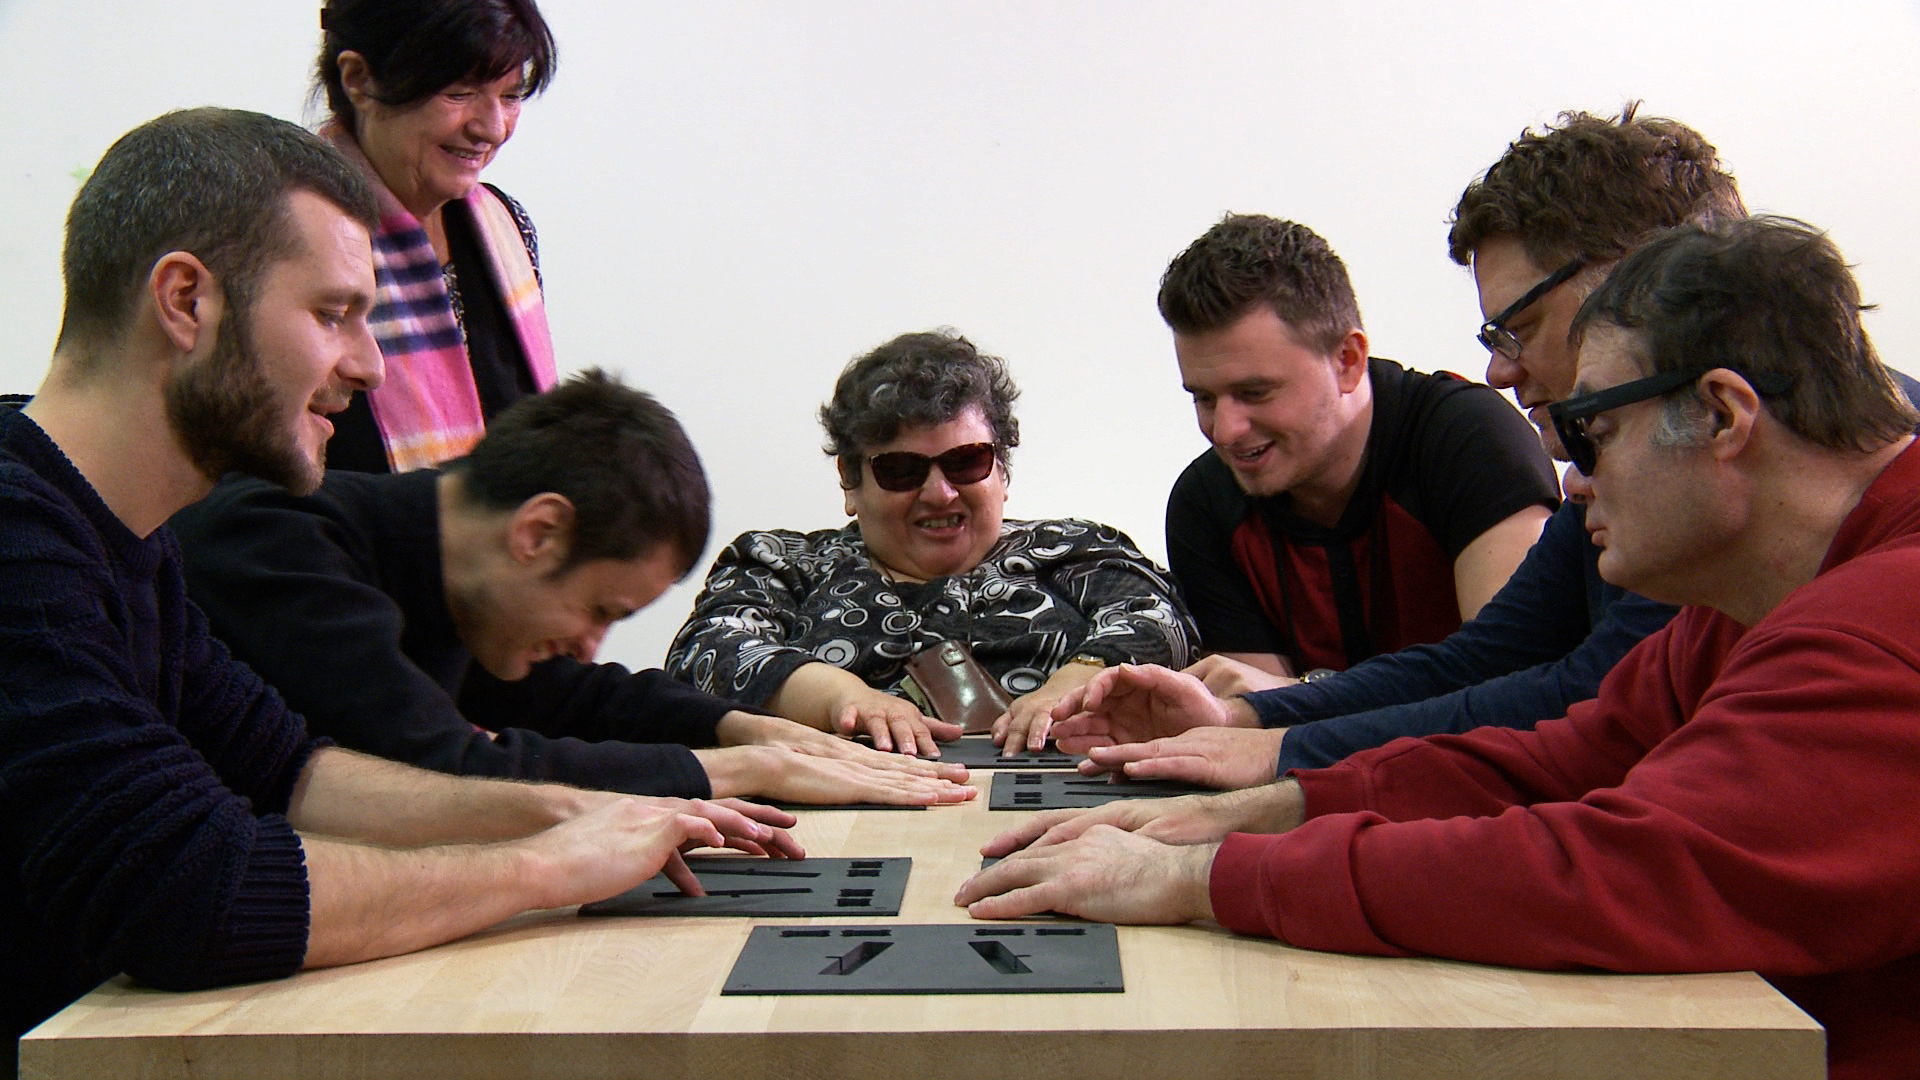
\includegraphics[width=\linewidth]{gfx/05_interfaces/tableSonotactile.jpg}
		\caption[La Table Sonotactile Interactive]{La Table Sonotactile Interactive : un dispositif interactif d'écoute installé à la Maison des Aveugles. Photographie © Anne Maregiano.}
		\label{fig:interface:tableSonotactile}
	\end{minipage}
	\hspace{.02\linewidth}
	\begin{minipage}[t]{0.48\textwidth}
	    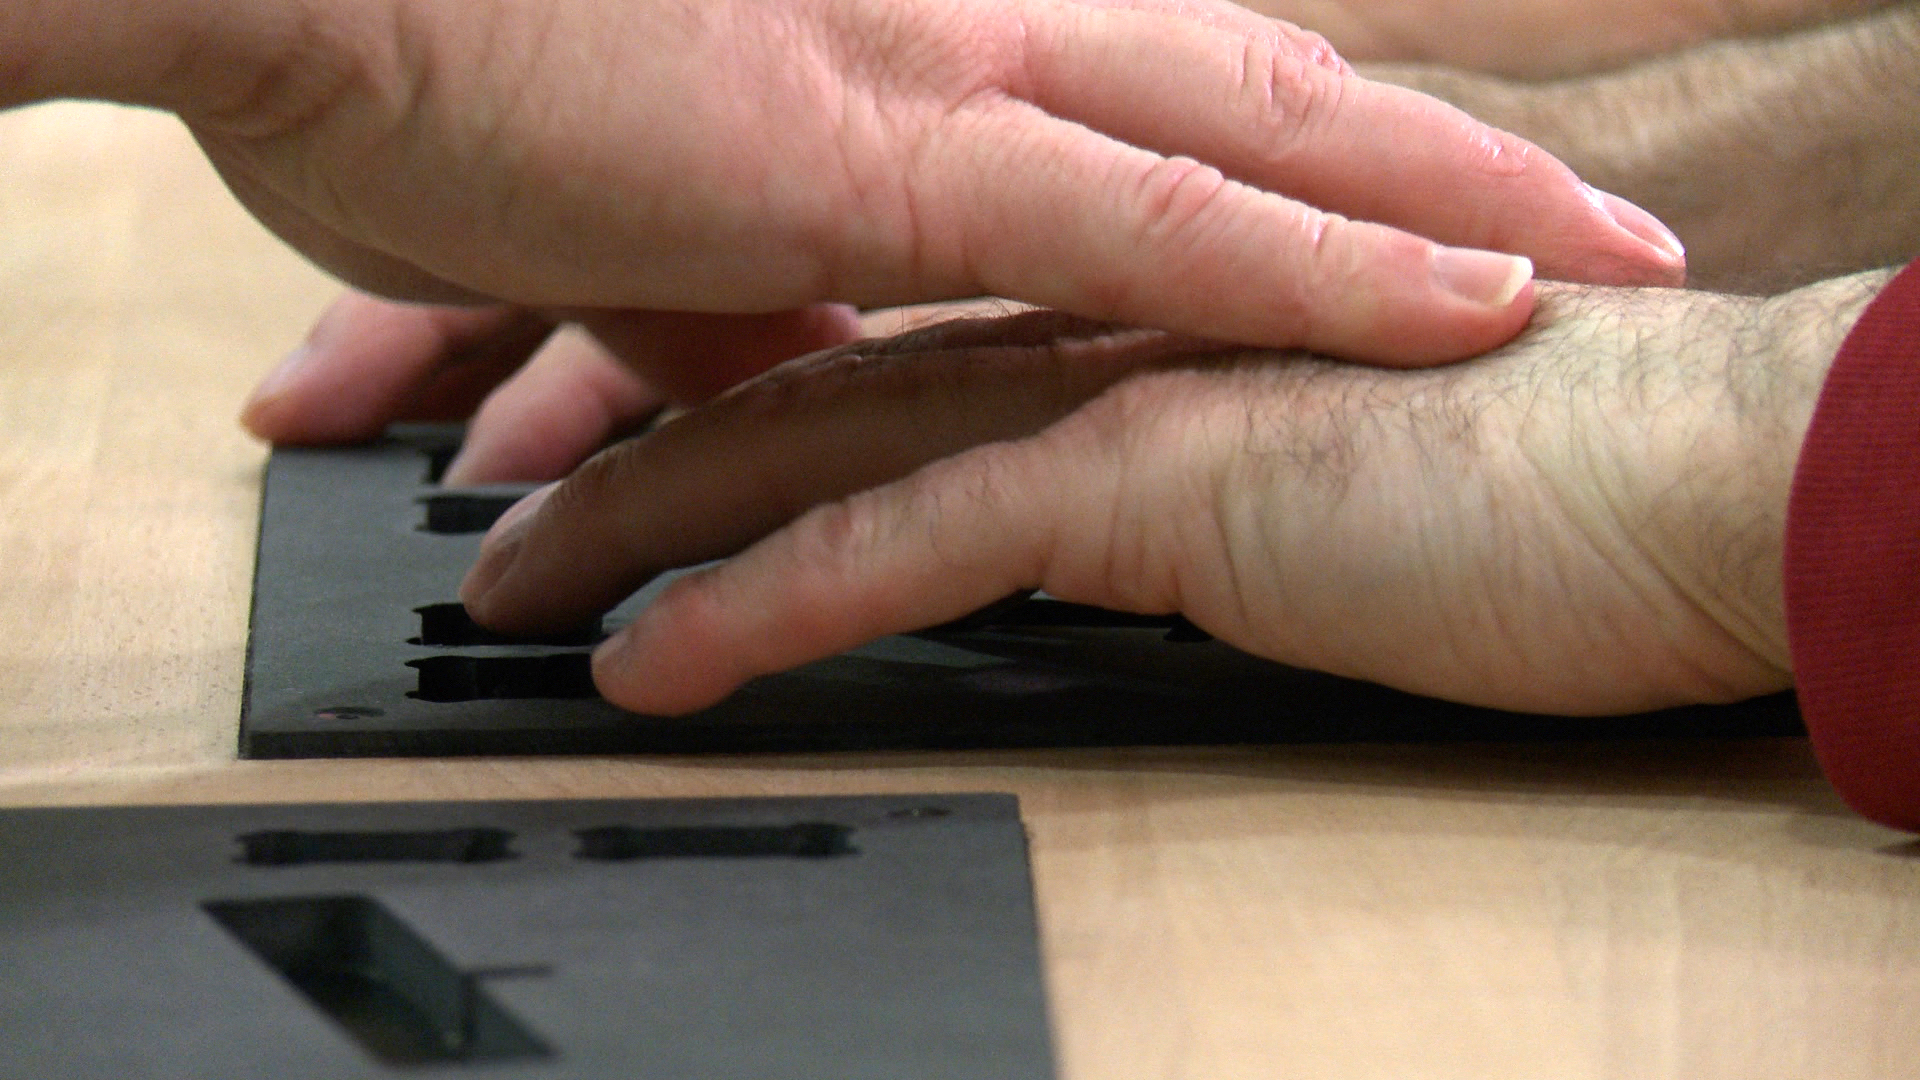
\includegraphics[width=\linewidth]{gfx/05_interfaces/tableSonotactile-pad.jpg}
		\caption[La Table Sonotactile Interactive : détail du pad]{La Table Sonotactile Interactive : détail du pad. Photographie © Anne Maregiano.}
		\label{fig:interface:tableSonotactile-pad}
	\end{minipage}
\end{figure}

\subsubsection{Repères tactiles}

\noindent L'état de surface des matériaux, la présence de reliefs (glissières, concavités, etc.) et de jeux mécaniques (e.g. l'enfoncement élastique d'une mousse recouvrant les pads \gls{MIDI}), contribuent à l'orientation tactile sur l'interface et à augmenter la cohérence entre le sens du toucher et la perception auditive des sons produits par le \gls{DMI}\footnote{Voir par exemple les glissères sur le pad d'interaction de la table sonotactile interactive, qui guident les doigts sur les potentiomètres linéaires, figure \ref{fig:interface:tableSonotactile-pad}}.\\
\indent Un grand défaut des interfaces graphiques dites ``tactiles'' est, ironiquement, que leur surface est généralement dépourvue de tels repères : aucune aspérité ne vient guider la main pour qu'elle trouve son chemin sur la matrice des capteurs, sans l'aide de la vue (ou de signaux sonores, comme vu ci-avant).\\
\indent Différentes stratégies présentées ci-après peuvent venir partiellement compenser cette lacune. Leur application dépend à la fois de la technologie de captation du \textit{multitouch}, ainsi que du type de repère, statique ou dynamique, que l'on souhaite.

\noindent\textbf{\textit{Repères statiques}}\\
\noindent Les surfaces multitouch permettent d'agencer de multiples zones virtuelles d'interaction : l'écran d'un smartphone présentent ainsi des boutons, des sliders, des menus, etc. activant des fonctions dissociées, sans qu'il soit tactilement possible de sentir leur contour. Les interfaces ``Joué''\footnote{\url{https://www.play-joue.com}} ou ``Sensel Morph''\footnote{\url{https://sensel.com}} commercialisent différents revêtements (\textit{overlays}) interchangeables pour leur surface \textit{multitouch}. Ces surfaces toutefois dépourvues d'écran graphique, ce qui évacue le problème de la transparence de ces repères. Une solution bon marché consiste à utiliser de la bande adhésive (cf. figure \ref{fig:interface:filigramophone-adhesif}). Un intermédiaire plus fin entre l'éphémère bande adhésive et une solution fixe consiste à utiliser une plaque de \gls{PMMA} (cf. figure \ref{fig:interface:filigramophone-plexigravure}) intermédiaire entre le doigt et la surface tactile, qui permet de graver des motifs potentiellement plus complexes. Cette dernière option n'est toutefois pas toujours réalisable sur les écrans à technologie capacitive, qui nécessite généralement que le doigt soit directement en contact avec l'écran.
%------------ Figure : repères statique -----------
\begin{figure}[!htbp]
	\captionsetup{format=plain}%
	\centering
	\begin{minipage}[t]{0.48\textwidth}
		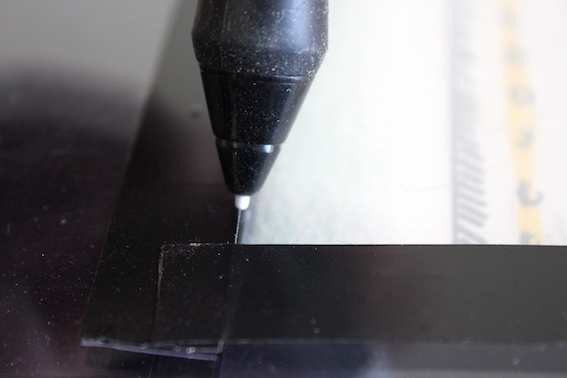
\includegraphics[width=\linewidth]{gfx/05_interfaces/filigramophone-adhesif_72dpi.jpg}
		\caption[Bande adhésive permettant de sentir le contour de la zone sensible de la tablette graphique dans le Filigramophone]{Bande adhésive permettant de sentir le contour de la zone sensible de la tablette graphique dans le Filigramophone.}
		\label{fig:interface:filigramophone-adhesif}
	\end{minipage}
	\hspace{.02\linewidth}
	\begin{minipage}[t]{0.48\textwidth}
	    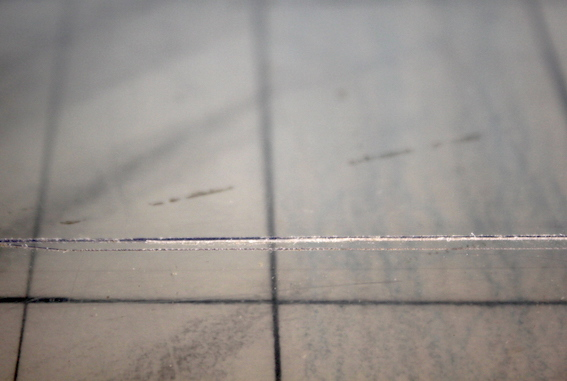
\includegraphics[width=\linewidth]{gfx/05_interfaces/Filigramophone_gravure_72dpi.jpg}
		\caption[Gravure d'une ligne médiane sur la plaque de PMMA du Filigramophone]{Gravure d'une ligne médiane sur la plaque de \gls{PMMA} du Filigramophone.}
		\label{fig:interface:filigramophone-plexigravure}
	\end{minipage}
\end{figure}

%------------ Figure : filigramophone et xypre piezo -----------
\noindent\textbf{\textit{Repères dynamiques : retours haptique et audiotactile}}\\
\label{sec:audio-fretting}
\noindent Les systèmes à retour haptique rendent tangible le contour, la résistance physique ou la vibration d'objets virtuels dynamiques. L'\gls{ACROE} a été pionnière dans cette direction appliquée à la lutherie numérique et développé à la fois des interfaces robotisées ainsi que les logiciels permettant une écriture musicale avec de telles interfaces. Plusieurs projets ont donné lieu à des prototypes d'écrans visuels intégrant un retour haptique, de manière globale \cite{sinclair_touchmover_2013}, ou distribué sur toute la surface par une matrice de mini-actionneurs \cite{follmer_inform_2013}. Des études ont démontré le bénéfice des interfaces haptiques sur l'évaluation qualitative de la relation instrumentale \cite{omodhrain_playing_2001, young_qualitative_2017}, mais la plupart d'entre elles restent encore à l'état de prototype et leur coût ainsi que la complexité de leur conception mécanique constitue souvent un facteur prohibitif.\\
\indent L'accessibilité des transducteurs tactiles, ainsi que la qualité de leur bande passante à considérablement augmenté depuis la dernière décennie et offre une alternative plus souple et économique pour la transmission d'information tactile. La solution la plus simple et directe pour établir un lien entre la perception auditive et tactile consiste à envoyer le résultat sonore (qui serait envoyé sur des haut-parleurs) dans le corps de l'instrument. Cette solution n'ajoute pas \textit{a priori} de repères autres que ceux perçu par les oreilles, mais la sensation vibratoire qui vient se coupler à la perception kinesthésique des gestes génère une sensation complexe perçue comme un tout cohérent, qui fusionne davantage encore que le simple couplage entre l'ouïe et la sensation kinesthésique, et qui semble aider la perception et la mémorisation spatiale de l'instrument. En particulier, utiliser le stylet d'une tablette graphique comme une tête de lecture, en associant sa position sur la tablette à la position temporelle de la lecture d'un échantillon sonore résulte en un troublant renversement des sens : la vibration recréé un état de surface fictif sur l'étendue de la tablette, qui donne l'impression d'être la cause du son entendu. D'autres essais ont été effectués dans la perspective d'améliorer la cohérence entre la sensation tactile et auditive. En particulier, l'accentuation des phénomènes transitoires, par un calcul différentiel du spectre pondéré par une courbe isosonique, semblait donner de meilleurs résultats. C'est assurément un champ riche et fertile, pour lequel différentes solutions sont envisageables et qu'il conviendrait d'étudier plus en profondeur.\\
\indent Un autre type de repère audiotactile qui s'inspire de cette expérience d'un état de surface virtuel, sans toutefois être aussi directement en relation avec le son audible, consiste à réaliser un ``frettage virtuel'' de la surface de jeu. L'envoi d'impulsions synchronisées à la position du stylet dans un transducteur tactile plaqué sur une tablette graphique, permet de simuler des petites ``bosses'' sur sa surface (un peu comme les frettes sur le manche d'une guitare). Ce frettage peut aider, par exemple, à sentir les paliers dans la progression d'un geste continu (e.g. les différentes ``notes'' d'une échelle de hauteur) (cf. figure \ref{fig:interface:virtual-fretting}) ou les contours d'une zone d'interaction\footnote{Cette technique permettant de simuler un relief par une simple vibration est notamment utilisée depuis 2015 dans les dernières version de boutons d'iPhone et de trackpad sur les ordinateurs portables Apple, une fonctionnalité connue sous le nom ``Force touch''.}.\\

%-------------------------- Figure : wacom ---------
\begin{figure}[!htbp]
	\captionsetup{format=plain}%
	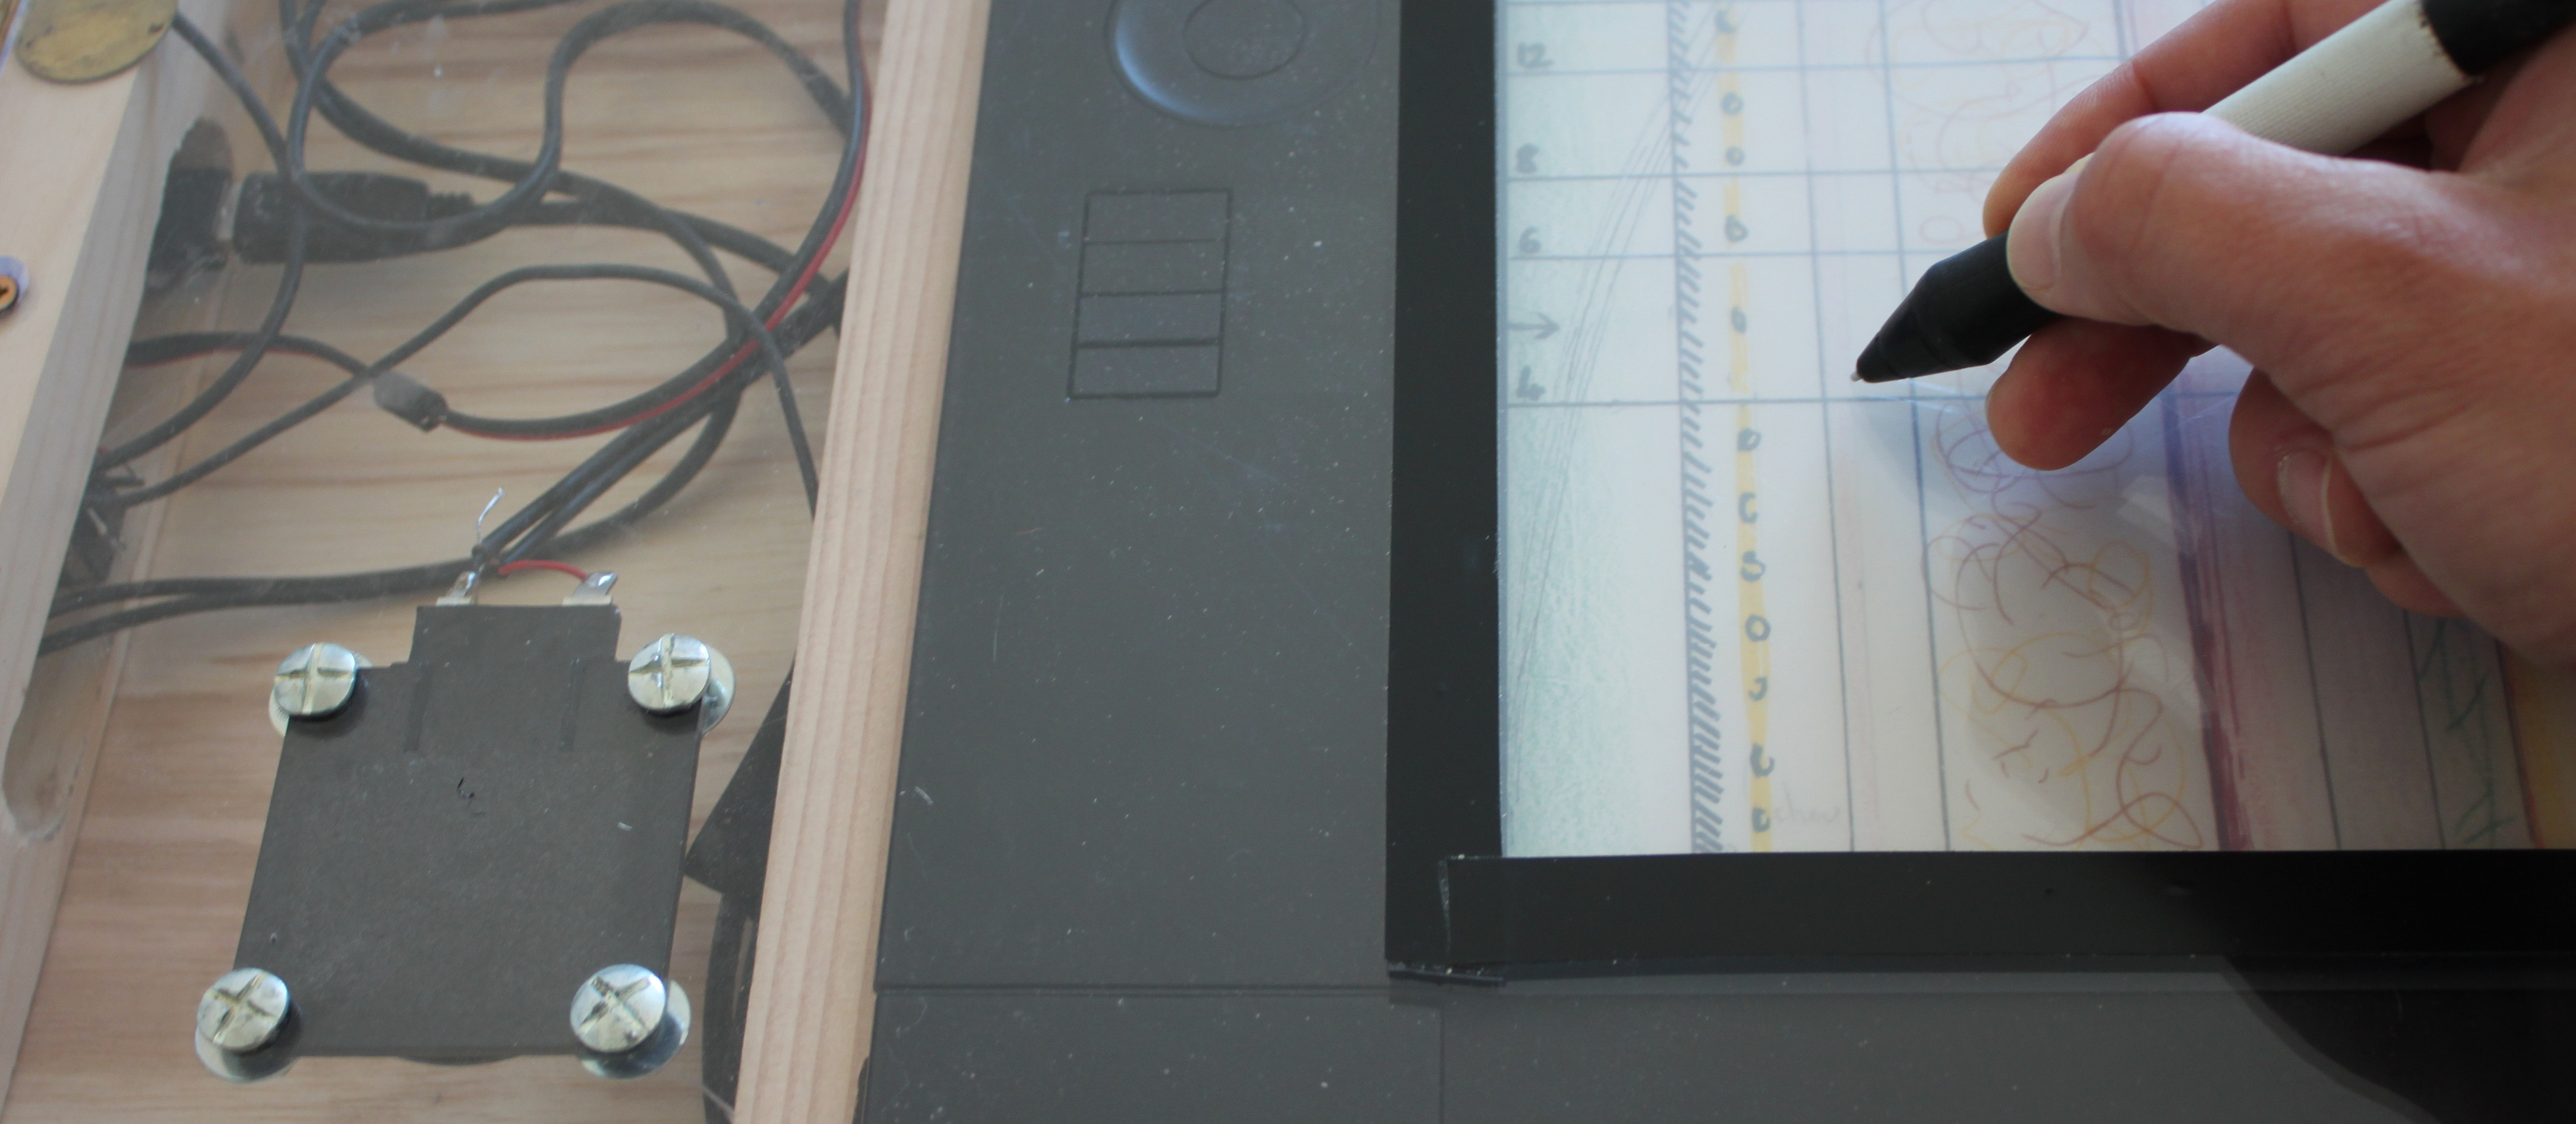
\includegraphics[width=\textwidth]{gfx/05_interfaces/virtual-fretting.jpg}
	\caption[Frettage virtuel par retour vibro-tactile]{Frettage virtuel par retour vibro-tactile: le transducteur tactile (en bas à gauche) émet une impulsion à chaque fois que le stylet franchit une frontière virtuelle (matérialisées par les lignes noires sur le calque).}
	\label{fig:interface:virtual-fretting}
\end{figure}
%-------------------------- Figure : wacom ---------


\noindent\textbf{Anamorphose dynamique}\\
\noindent Enfin, il est possible de procéder algorithmiquement à des anamorphoses de l'espace de jeu. Cette solution ne permet pas de ``créer'' des repères tactiles à proprement parler, mais d'adapter dynamiquement l'espace de l'interaction pour que le geste puisse s'affranchir en partie du besoin de ces repères.\\
\indent Un exemple classique est le verrouillage des composants d'une \gls{GUI} pendant l'interaction: si l'on clique sur un bouton ou un \textit{slider}, l'interaction est maintenue avec le composant tant que le doigt est en contact avec la surface tactile, ce qui permet des gestes plus amples utilisant l'intégralité de la surface de l'écran tactile, plutôt que de les restreindre à une petit zone\footnote{Cette solution a notamment été implémentée dans la librairie mp.TUI présentée au chapitre \ref{ch:visual_representation}.}. Cette stratégie d'interaction s'appuie sur la loi de Fitts \cite{fitts_information_1954}, caractérisant \textit{l'indice de difficulté} d'une tâche de sélection par pointage, couramment exprimée en terme de temps mis à réussir ce pointage, par la relation (formulation de MacKenzie): 
$$ T = a + b \log_2 (1 + \frac{D}{L})$$
\vspace{-1em}
\begin{conditions}
$T$     	& temps moyen pris pour effectuer le mouvement; \\
$D$			& distance séparant le point de départ du centre de la cible;\\
$L$			& largeur de la cible mesurée selon l'axe de mouvement;\\
$a, b$  	& variables pouvant être déterminés empiriquement.
\end{conditions}

\noindent Un autre exemple d'anamorphose, plus directement lié au domaine musical, est l'algorithme de correction dynamique de la hauteur\footnote{L'algorithme s'applique à la hauteur, comme à n'importe quel autre paramètre qu'il pourrait être intéressant de contrôler à la fois de manière continue et discrète.} à l'attaque, présenté dans \cite{goudard_playing_2014} et sur la figure \ref{fig:algorithms:MID-dynamic-pitch-correction}.

\subsubsection{Repères somesthésiques}

\noindent Enfin, le développement des réflexes moteurs qui permettent la virtuosité de jeu sur une interface passe par une cognition incarnée, qui s'appuie sur notre perception \textit{somesthésique}, c'est-à-dire l'ensemble des sensations internes du corps. En particulier, parmi les différents sensations que recouvrent la somesthésie, la \textit{proprioception} désigne la perception de la position des différentes parties de notre corps dans l'espace, recouvrant le sens du mouvement (\textit{kinesthésie}) et le sens de la posture (\textit{statesthésie}). La somesthésie est particulièrement mise à contribution dans les \glspl{DMI} qui ne présentent pas d'interface physique tangible, tels que ceux basés sur des gestes libres (e.g. captés par une Kinect), et peut s'avérer être la seule sensation directe (i.e. non médiatisée par la machine) disponible dans les \glspl{DMI} basés sur les signaux biologiques (e.g. tension des muscles du Myo).\\
\indent Durant la phase de conception d'un \gls{DMI}, cette exploration est double : il s'agit à la fois d'intégrer la topologie physique de l'instrument (disposition des capteurs, espace du mouvement autour de ceux-ci, course sensible et courbes de réponse...) mais également la topologie virtuelle des algorithmes manipulés, c'est à dire la redistribution dynamique de cette spatialité pendant le jeu musical. Par exemple, dans le cas de la manipulation d'un modèle intermédiaire dynamique\footnote{Cf. section \ref{sec:algorithms:MID}} (e.g. un bâton de pluie virtuel), le résultat d'un même geste pourra différer en fonction de l'état du modèle intermédiaire (selon que les grains de sâble du bâton de pluie sont d'un côté ou de l'autre).\\
\indent Ainsi, le positionnement des capteurs dans l'interface \textit{Xypre} a été revu en fonction de gestes qui venaient naturellement lors du jeu avec le \textit{Filigramophone}. Par exemple, le geste de percussion sur le côté du châssis venait naturellement dans la course du bras pivotant autour de l'articulation de l'épaule, alors qu'aucun capteur n'avait été positionné là. C'est par ailleurs un geste de percussion qu'on retrouve dans des instruments de percussion comme le Mridang indien, et que l'auteur ayant pratiqué le tabla trouvait relativement aisé.

% [extra]:\\
% correspondance entre l'anatomie corporelle et celle de l'interface\\
% \iquote{Though there is a huge range of performer decision, history, and knowledge that will determine their exact method of playing (as established by Jorda [12]), the physical design of the DMI impacts this gesture repertoire by presenting certain affordances.} \cite{bin_hands_2017}


%------------------------------------------------------------
\subsection{Ergodynamie}

\noindent Les différents aspects qui contribuent à l'ergonomie de l'interface de jeu d'un \gls{DMI} sont ainsi à la fois ancrés dans le corps matériel de l'instrument, mais également dans les artéfacts sonores, visuels ou vibratoires produits par l'ordinateur. À ces aspects cognitifs s'ajoute l'expérience personnelle et la reconnaissance de tous les éléments appartenant au répertoire culturel dans lequel un nouveau \gls{DMI}, encore inconnu, s'inscrit.\\
\indent Thor Magnusson propose la notion d'\textit{ergodynamie} \iquote{comme un terme qui s'approche d'une certaine manière de l'usage du mot `gameplay' dans le domaine des jeux vidéo, mais qui traduit également une conscience et une expérience de l'instrument dans des pratiques incarnées, historiques et esthétiques. L'ergodynamie concerne l'objet étudié, mais elle se rapporte aussi bien au contexte culturel qu'à des expériences personnelles subjectives de cet objet.}\footnote{\iquote{(...) the word \textit{ergodynamics} is proposed as a term that somewhat relates to the use of ‘gameplay’ in computer games, but further signifies an awareness and experience of the instrument in embodied, historical, and aesthetic practices. Ergodynamics are of the object studied, but it relates equally to cultural context and subjective personal experiences of it.} \cite{magnusson_ergodynamics_2019}.}


%%%%%%%%%%%%%%%%%%%%%%%%%%%%%%%%%%%%%%%%%
\section{Un exemple pratique : phylogenèse d'interfaces de type tablette}
\label{sec:interfaces:phylogenese}

\noindent Cette partie retrace le développement d'une série d'interfaces de \glspl{DMI}, basée sur un archétype d'instrument de type ``tablette''. On peut voir dans la tablette graphique des liens évidents avec les gestes du dessin et de l'écriture, tandis que l'usage généralisé des écrans \textit{multitouch} sur les smartphones a fait émergé un grand nombre d'habitudes d'interaction (ainsi que les attentes que ces habitudes génèrent) telles que les mouvements de balayage, de \textit{pinch-to-zoom}, de défilement à deux doigts, etc.\\
\indent La conception d’une nouvelle interface pour la performance musicale est une tâche complexe, nécessitant de nombreux aller-retours entre conception, fabrication et pratique musicale. Le filigramophone est une interface qui a connu plusieurs versions, suffisamment différentes pour les considérer comme des instruments distincts et suffisamment similaires pour y voir la continuité d’une seule et même famille d'instruments.

%----------------------------------------------------------------------------------------------------------
\subsection{Origine : la tablette graphique (2005)}
\label{sec:interfaces:phylogenese:wacom}

\noindent La tablette graphique (précisément un modèle Sapphire de Wacom) a été l’interface originelle qui a servi de base au filigramophone. J’ai commencé à l’utiliser dans le cadre du développement de la Méta-Mallette\footnote{Logiciel pour la pratique collective de musique par ordinateur développé par l’association Puce Muse, au développement duquel j'ai activement participé entre 2005 et 2008.}. Le choix de cette interface était motivé par la diversité de gestes expressifs possibles sur une tablette graphique, ainsi que par son coût relativement abordable\footnote{un peu moins de 100€ en 2005, autour de 50€ pour un modèle équivalent en 2019.} comparativement à la plupart des interfaces \gls{MIDI}, permettant de la déployer en nombre, dans le cadre d'activités pédagogiques pratiquées en groupe, dans des écoles et autres collectivités.\\
%------------ Figure : fairlight CMI et UPIC -----------
\begin{figure}[!htbp]
	\captionsetup{format=plain}%
	\centering
	\begin{minipage}[t]{0.48\textwidth}
		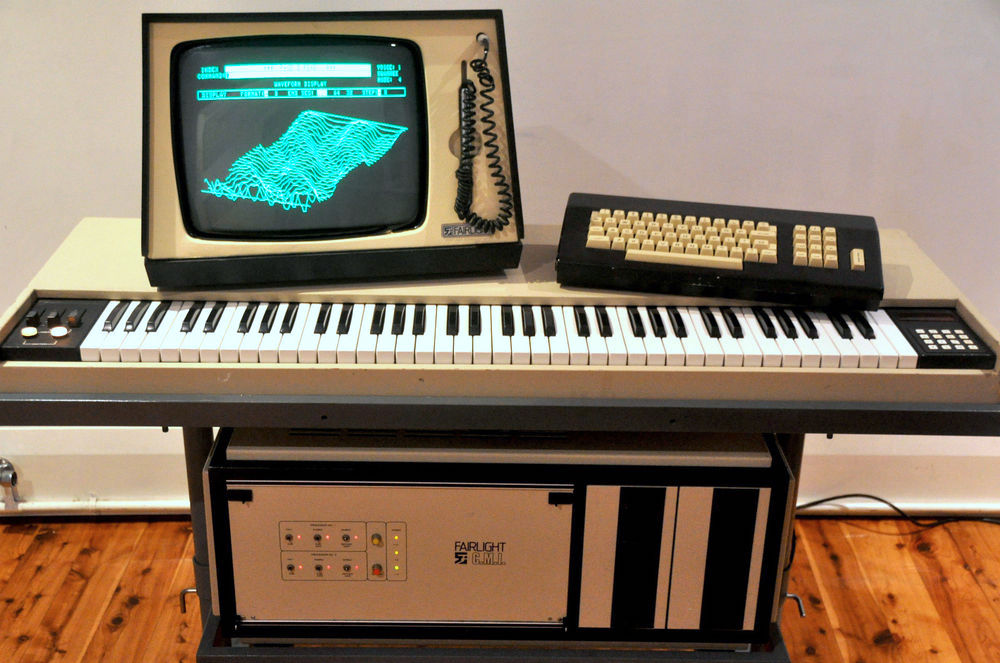
\includegraphics[width=\linewidth]{gfx/05_interfaces/fairlight-CMI.jpg}
		\caption[Le Fairlight CMI]{Le \textit{Fairlight CMI} créé en 1976, un synthétiseur et séquenceur utilisant un écran à stylet. Photographie : Peter Wielk.}
		\label{fig:interface:fairlightCMI}
	\end{minipage}
	\hspace{.02\linewidth}
	\begin{minipage}[t]{0.48\textwidth}
	    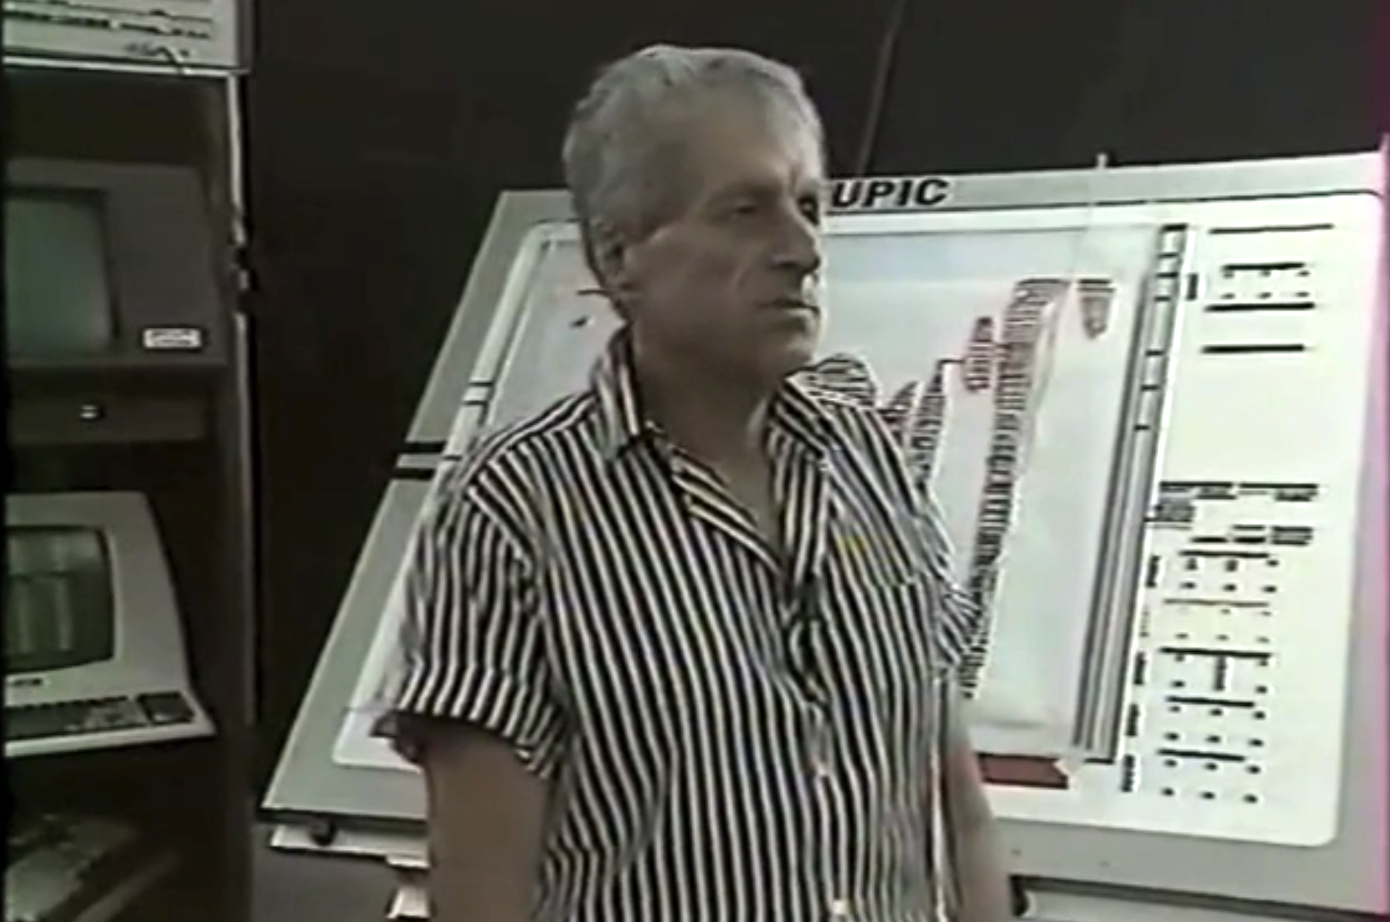
\includegraphics[width=\linewidth]{gfx/05_interfaces/UPIC-Xenakis.png}
		\caption[L'UPIC de Iannis Xenakis]{La station UPIC inventée par Xénakis permet de dessiner des formes graphiques libres, pouvant être lues de différentes manières pour être traduites en son. (Image extraite du documentaire ``Avenir UPIC Xenakis'', centre Xénakis)}
		\label{fig:interface:UPIC}
	\end{minipage}
\end{figure}
\index[people]{xenakis@Xénakis, Iannis}
%------------ Figure : fairlight CMI et UPIC -----------
\indent À l'origine destinée aux graphistes, les tablettes à stylet ont également été utilisées pour la composition. Le système \textit{UPIC} inventé par Iannis Xénakis (figure \ref{fig:interface:UPIC}) ou le \textit{Fairlight CMI}  (figure \ref{fig:interface:fairlightCMI}) utilisaient tous les deux, dans des directions relativement différentes, une interface basée sur la tablette et le stylet. En dehors de son usage pour la composition, un certain nombre de musiciens, compositeurs et concepteurs de \gls{NIME} l’ont par ailleurs adoptée pour la performance\footnote{Notamment à l'\gls{IRCAM} (voir \cite{wanderley_choice_2000}), au \gls{CNMAT} (voir \cite{zbyszynski_ten_2007}, au \gls{LMA} \cite{couturier_utilisation_2004}, au \gls{LIMSI} \cite{feugere_chorus_2011} puis dans l'équipe \gls{LAM} \cite{xiao_t-voks_2019}, mais on peut également citer Pierre Jodlowski\index[people]{Jodlowski, Pierre@} (voir \url{https://youtu.be/pLARXmGwIO4}) ou Jesper Nordin\index[people]{Nordin, Jesper@} (voir \url{https://gestrument.com}).}. Nicolas d’Alessandro a consacré une partie de son travail de thèse \cite{dalessandro_realtime_2009} à ce sujet, en proposant une étude détaillée des différentes échelles de mouvements dans le geste du dessin et de l'écriture, liées à l'articulation entre doigts, poignet et épaule. J'avais pour ma part utilisé la tablette graphique dans différents projets\footnote{\textit{filigram}, \textit{Media Music rooM}, cf. \url{http://vincentgoudard.com}}, comme un composant parmi d'autres interfaces \gls{MIDI} ou de type joystick, avant de développer plus particulièrement des programmes pour cette interface.\\
\indent Un des inconvénient de la tablette Wacom est que les contours de la surface utile, plus petite que la surface de la tablette\footnote{Cela permet de ne pas ``tomber'' hors de la tablette.}, sont à peine perceptibles, tant visuellement qu'au niveau tactile. Cela s'avère problématique quand on manipule certains processus sonores (et non un pinceau dans PhotoShop, tel que l'usage de la tablette le prévoit), car le regard de l'instrumentiste est souvent déjà occupé par l'attention qu'il/elle aux autres instrumentistes, à une partition, ou un chef d'orchestre. Une première adaptation a donc consisté à rajouter des bandes adhésives permettant de matérialiser cette frontière, visuellement et tactilement (cf. figure \ref{fig:interface:wacom}).\\
%-------------------------- Figure : wacom ---------
\begin{figure}[!htbp]
	\captionsetup{format=plain}%
	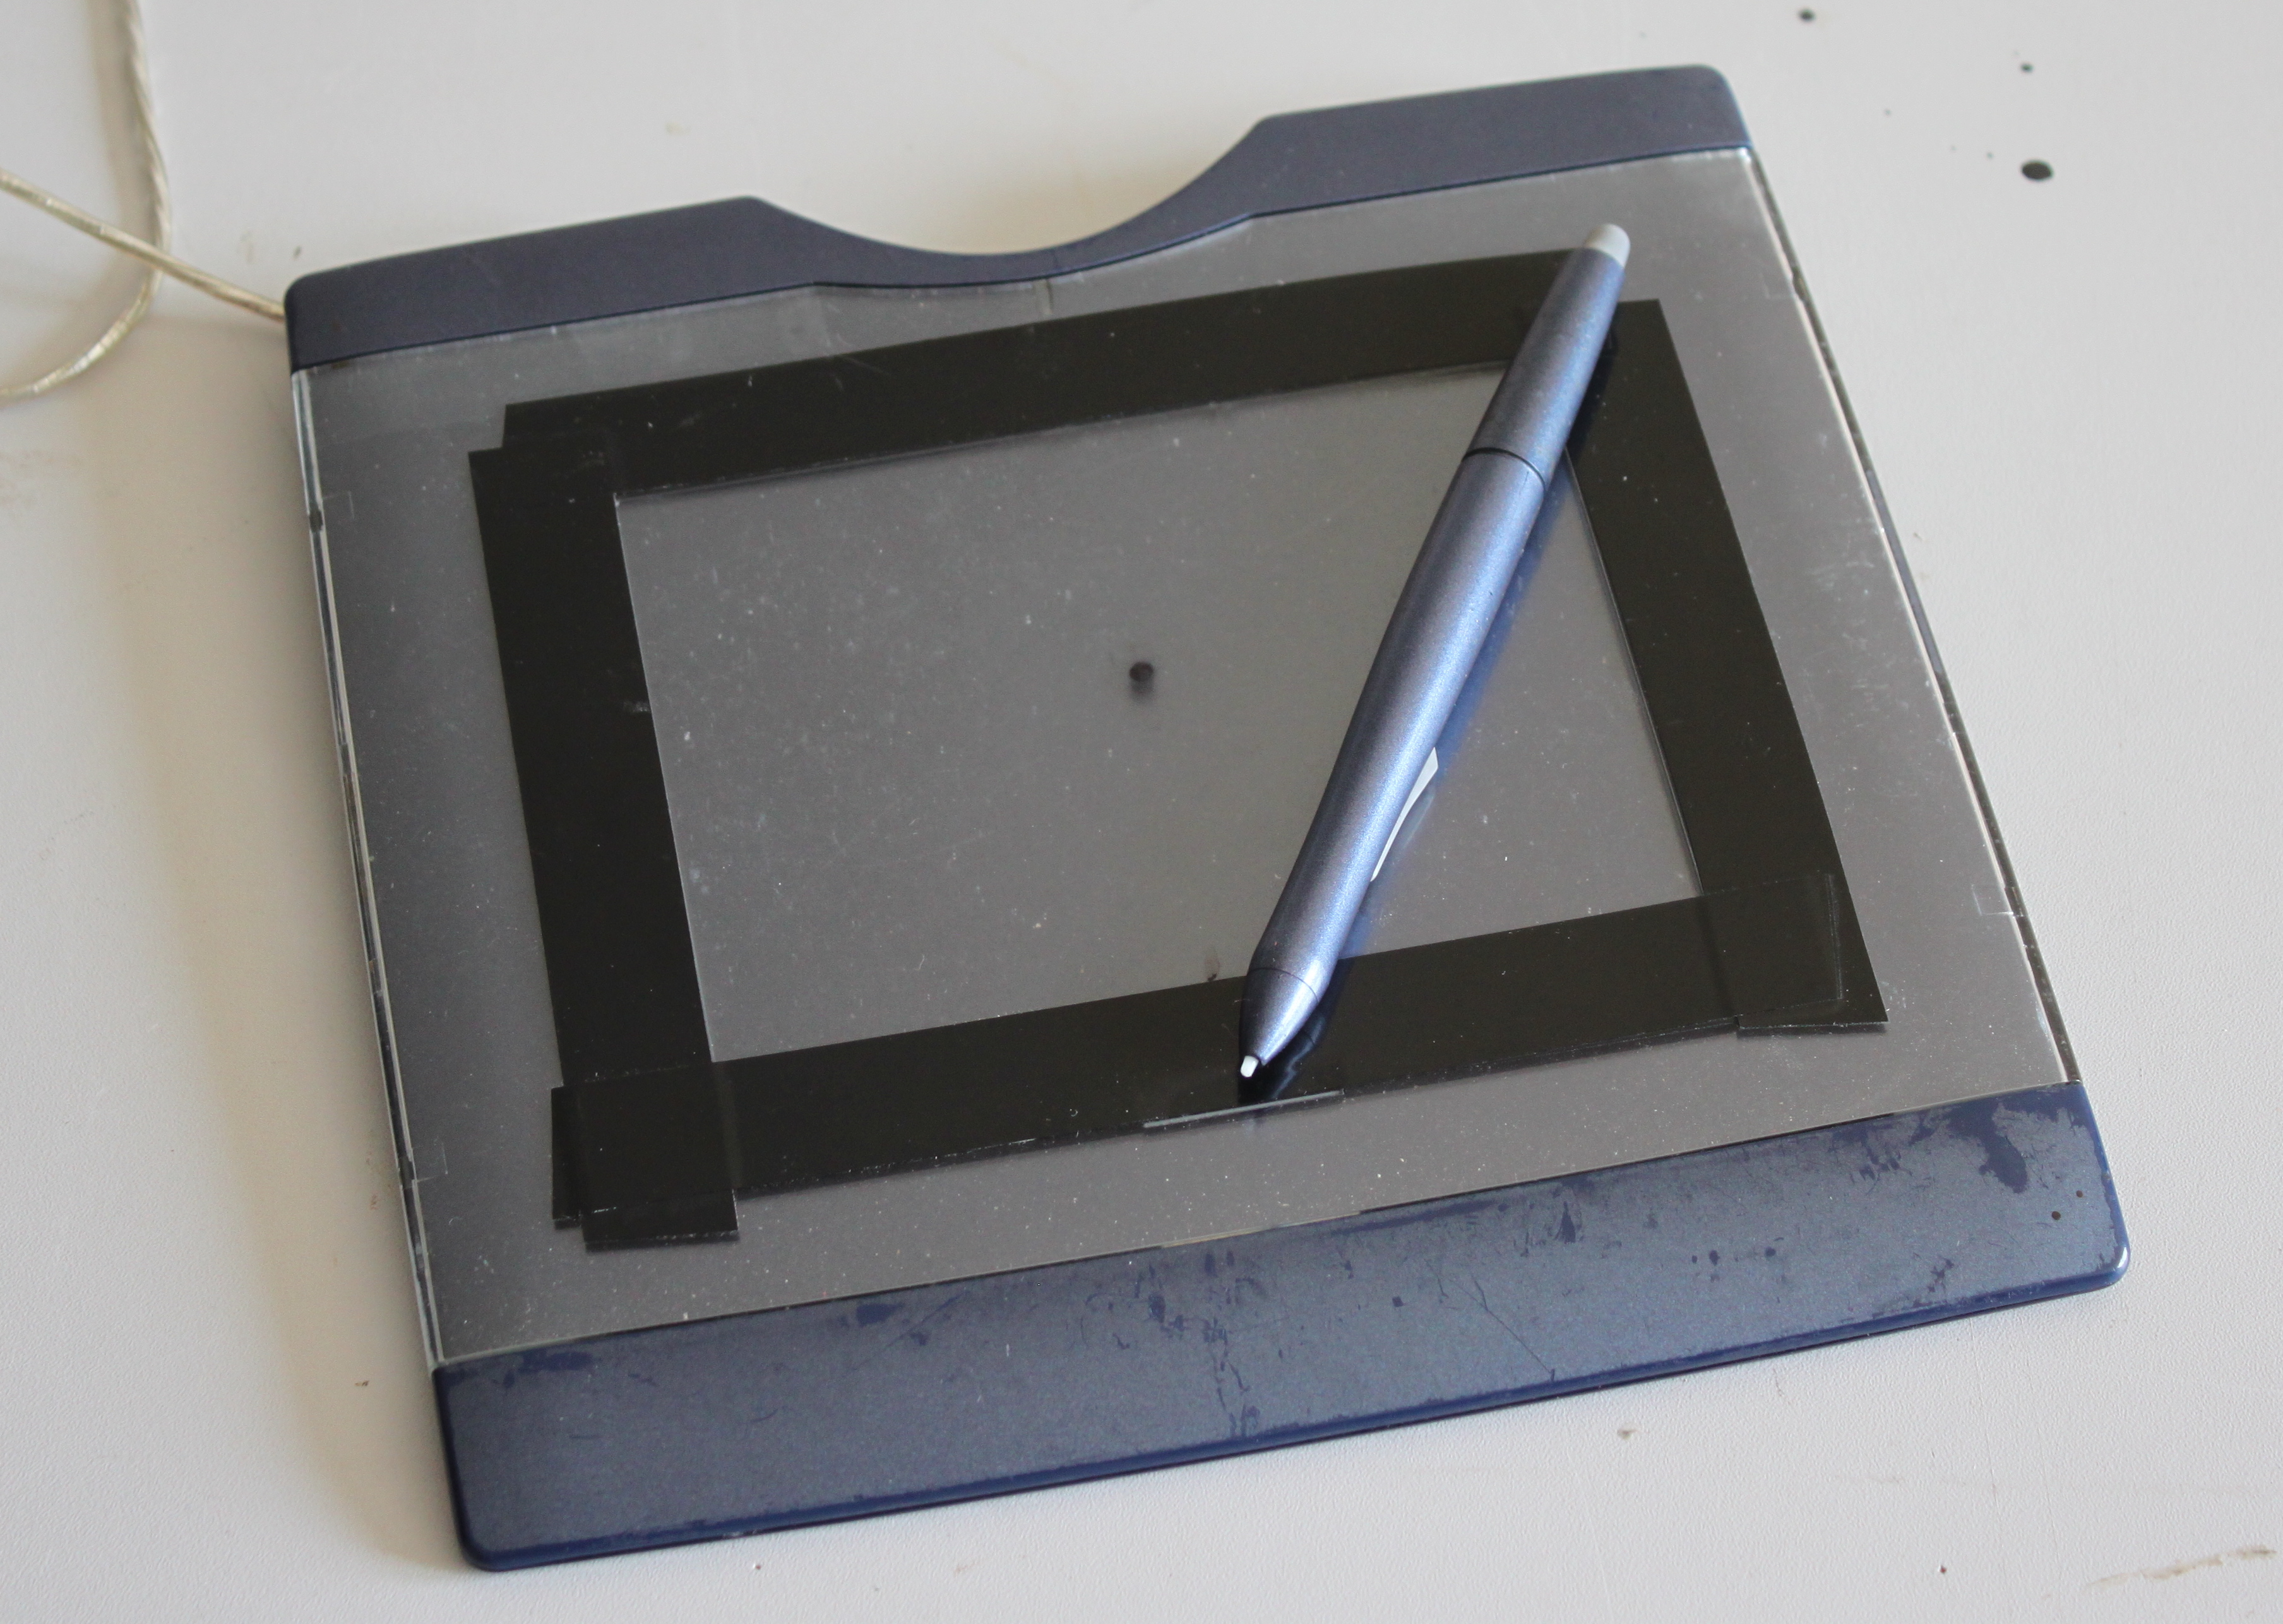
\includegraphics[width=\textwidth]{gfx/05_interfaces/wacom.jpg}
	\caption[Tablette wacom]{Tablette Wacom utilisée à l'origine. Des adhésifs rajoutés en bordure guident la perception haptique, un point central sert de repère visuel.}
	\label{fig:interface:wacom}
\end{figure}
%-------------------------- Figure : wacom ---------
\indent En 2007, dans l'équipe \gls{LAM}, Hugues Genevois avait acquis de nouveaux transducteurs tactiles large bande\footnote{Cette nouvelle génération offrait une bande passante de l'ordre du Hz jusqu'à plusieurs kHz, bien supérieure aux actuateurs linéaires, ainsi qu'une dynamique supérieure à celle des transducteurs piezo. Cette technologie a depuis équipé de nombreux cinémas pour donner au spectateur une expérience plus tactile du son.}. Nous avons fait l'expérience d'en placer un sous une tablette graphique, sur laquelle nous contrôlions la lecture d'un échantillon en se servant du stylet comme d'une tête de lecture virtuelle. La sensation haptique résultant était tout à fait saisissante et donnait l'impression que la surface de la tablette avait un relief physique similaire aux reliefs perçus dans le son : littéralement, l'impression de ``toucher le son''. Ce ``relief'' artificiel est bien entendu éphémère car ces transducteurs ne transmettent pas le continu et leur course est faible\footnote{Ceci les différencie nettement des systèmes de retours haptiques tels que développés, en particulier, à l'\gls{ACROE}.}, mais la sensation est tout à fait confondante. J'ai donc utilisé ce système directement sur la tablette graphique, qui était une sorte de prototype du Filigramophone présenté ci-après.

%----------------------------------------------------
\subsection{Le Filigramophone: une tablette augmentée (2013)}
\label{sec:interfaces:phylogenese:filigramophone}

%-------------------------- Figure : filigramophone ----------------------------------
\begin{figure}[!htbp]
	\includegraphics[width=\textwidth]{gfx/filigramophone/filigramophone_overview.jpg}
	\caption[Filigramophone - vue d'ensemble, débranchée]{Filigramophone - vue d'ensemble, débranchée.}
	\label{fig:interface:filigramophone}
\end{figure}
%----------------------------------------------------------------------------------------------------------
\noindent L'expérience décrite précédemment a suscité le développement d'une interface plus intégrée, augmentant la tablette graphique d'une dimension acoustique bi-directionnelle, en captant d'une part le son de la tablette à l'aide de microphones piezo et en diffusant des signaux audio dans la tablette à l'aide de transducteurs tactiles.

\subsubsection{Intégration des microphones piezo}

\noindent En effet, si la tablette graphique est une interface relativement expressive, par la possibilité qu'elle offre de contrôler trois, voire cinq variables continues en même temps\footnote{La position horizontale et verticale, la pression, et sur certains modèles, l'inclinaison du stylet selon les deux axes.}, sa fréquence d'échantillonage reste relativement faible\footnote{Généralement de 100Hz, d'après Wacom, mais l'objet wacom recevant les données de manière asynchrone dans Max ne permet pas la pleine exploitation de cette fréquence.} et la latence importante\footnote{La latence entre le mouvement du stylet et l'arrivée des données est de l'ordre de 50ms, alors qu'elle est de l'ordre de 5ms pour le \gls{MIDI}.}. Le désir de l'augmenter de microphones est ainsi largement lié à cette sensation de distance, qu'on retrouve de manière générale dans la plupart des interfaces de contrôle de type \gls{MIDI} (bien que moindre dans le \gls{MIDI}, cette distance est également sensible).\\
\indent Ali Momeni\index[people]{momeni@Momeni, Ali} avait réalisé ce type d'augmentation acoustique, en plaçant un microphone piezo directement sur la tablette\footnote{Développements présentés dans sa thèse \cite{momeni_composing_2005}.}. Cette technique lui permet de \iquote{Taper, gratter, frapper avec un anneau métallique ou frotter la tablette} pour obtenir une variété de signaux audio captés par le microphone piezo.\\
\indent Plus récemment, Romain Michon a étudié différentes possibilités d'effectuer des gestes percussifs et de pression sur une tablette \textit{multitouch}\footnote{Voir \cite{michon_nuance_2016}.}, et proposé une solution hybride par l'ajout de capteurs \gls{FSR} placés sous un iPad, modulés en amplitude et récupérés via l'entrée audio d'un iPad. L'intérêt de cette solution est de permettre le calcul de la vélocité des gestes percussifs, en plus de l'aftertouch, mais la fusion des informations de pression et de coordonnées X/Y, bien que judicieusement contournée par une triangulation des différents \gls{FSR}, reste problématique comme le remarque son auteur. Par ailleurs, cette solution utilisant des capteurs de pression, sous la surface rigide de l'iPad ne permet pas d'exploiter la variation de hauteur spectrale en fonction du lieu de frappe, la surface de l'iPad étant trop rigide et les \gls{FSR} inadaptés à cette gamme de fréquences.\\
%------------ Figure : filigramophone et xypre piezo -----------
\begin{figure}[!htbp]
	\captionsetup{format=plain}%
	\centering
	\begin{minipage}[t]{0.48\textwidth}
		\includegraphics[width=\linewidth]{gfx/05_interfaces/filigramophone-piezo_72dpi.jpg}
		\caption{Transducteur piezo entre la vitre et le châssis sur le Filigramophone}
		\label{fig:interface:filigramophone-piezo}
	\end{minipage}
	\hspace{.02\linewidth}
	\begin{minipage}[t]{0.48\textwidth}
		\includegraphics[width=\linewidth]{gfx/05_interfaces/filigramophone_hp_72dpi.jpg}
		\caption{HP tactile sur le Filigramophone}
		\label{fig:interface:filigramophone-hp}
	\end{minipage}
\end{figure}
%------------ Figure : filigramophone et xypre piezo -----------
\indent J'ai pour ma part choisi d'insérer les microphones piezo entre une vitre en \gls{PMMA} et le châssis contenant la tablette graphique (cf. figure \ref{fig:interface:filigramophone-piezo}). Cela permet des gestes percussifs, de frottements ou l'utilisation d'objet mis en mouvement (toupies, dés, disques, etc.) directement sur la surface, tout en conservant --~à travers le \gls{PMMA}~-- l'usage de la tablette qui renvoie les coordonnées horizontale et verticale ainsi que la pression et l'inclinaison du stylet. Ces transducteurs piezo permettent de capter les différents timbres de la surface \gls{PMMA}, qui présente une certaine élasticité (par rapport à la surface rigide de la tablette) en étant fixée uniquement sur ses bords, et dont la hauteur spectrale est plus grave au centre et plus aigüe sur les bords, à la manière d'une peau de tambour. Il est également possible de frapper sur le châssis, ce qui permet d'obtenir encore d'autres nuances de timbre (figure \ref{fig:interface:filigramophone-toupie}). Cette solution évite par ailleurs les bruits ``parasites'' de la structure de la tablette graphique quand on frappe directement dessus. Enfin, l'ajout de la plaque de \gls{PMMA} laisse la possibilité de dessiner, ajouter de l'adhésif, ou graver directement directement sur le \gls{PMMA}, sans détériorer la tablette. Eventuellement, disposer de différentes plaques de \gls{PMMA} permettrait d'adapter l'interface à différentes configurations, à la manière des ce que permettent les \textit{overlays} sur les interfaces commerciales \textit{Joué} et \textit{SenselMorph}\footnote{\url{https://www.play-joue.com}, \url{https://sensel.com}.}, ou à des compositions différentes, telles que les ``\textit{tangible scores}'' d'Enrique Tomás \cite{tomas_tangible_2014}.

%-------------------------- Figure : filigramophone-toupie ----------------------------------
\begin{figure}[!htbp]
	\captionsetup{format=plain}%
	\includegraphics[width=\textwidth]{gfx/05_interfaces/filigramophone-toupie.jpg}
	\caption[Captation du son des mains ou d'objets sur la surface du Filigramophone]{Le microphone piezo laisse la possibilité de capter le son des mains ou d'objets sur la surface du Filigramophone}
	\label{fig:interface:filigramophone-toupie}
\end{figure}
%-------------------------- Figure : filigramophone-toupie ----------------------------------

\subsubsection{Intégration du transducteur tactile}

\noindent Parallèlement, un transducteur a été fixé sur la vitre de \gls{PMMA} (cf. figure \ref{fig:interface:filigramophone-hp}), et positionné empiriquement\footnote{c'est-à-dire, par un balayage des fréquences, envoyé sur le transducteur, en écoutant et en touchant la surface pour y trouver les zones de résonance.} pour favoriser l'excitation des premiers modes de résonance de la plaque de \gls{PMMA} sans être toutefois dans la zone d'interaction de la tablette graphique. Les premiers modes de résonance correspondent en effets aux fréquences les plus basses, et le but était ici d'avoir une vibration aussi forte que possible dans un domaine vibrotactile qui n'empiète pas trop sur le domaine audible.\\
\indent Le transducteur tactile est utilisé à la fois pour le retour vibratoire et la communication d'information, en particulier par frettage virtuel de la surface (cf. infra, section \ref{sec:audio-fretting}). Le retour vibratoire de l'instrument se distingue toutefois de l'envoi pur et simple du signal audio, la perception tactile ne lui étant pas directement liée. Au lieu de cela, un signal sinusoïdal à 70Hz, correspondant à une fréquence de résonance de la vitre de \gls{PMMA}, modulé par l'enveloppe du son final, ainsi que par sa dérivée spectrale, afin de mieux sentir dans les doigts les transitions et les ruptures du son.\\
%(cf. figure TODO : schéma de principe du patch / développement dans une autre partie ?).\\
\indent Le Filigramophone a été joué plusieurs fois en concert, à la fois dans l'ensemble ONE, ainsi que dans la première version de la performance audio-visuelle ``FIB\_R'' avec la plasticienne Gladys Brégeon (cf. figure \ref{fig:interface:filigramophone-Xypre-Triton}). Le dispositif complet était composé du Filigramophone, d'un ordinateur faisant tourner un patch Max pour la synthèse, d'une carte son et haut-parleurs, ainsi que d'une interface \gls{MIDI} Akai MPD24, donnant un accès direct à davantage de paramètres tels que le volume général, le mixage entre différentes synthèses, le rappel de configurations, la sélection d'échelles musicales pour l'accordage, ainsi que divers autres paramètres spécifiques aux algorithmes de synthèse.

%-------------------------- Figure : fibroscopie Triton ----------------------------------
\begin{figure}[!htbp]
	\captionsetup{format=plain}%
	\includegraphics[width=\textwidth]{gfx/05_interfaces/fibroscopie-Triton.jpg}
	\caption[Filigramophone et prototype du Xypre sur scène]{Filigramophone (à droite) et une version prototypique du Xypre v1 (à gauche) sur scène, durant la répétition de FIB\_R en juin 2015, Le Triton, Les Lilas (93).}
	\label{fig:interface:filigramophone-Xypre-Triton}
\end{figure}
%-------------------------- Figure : fibroscopie Triton ----------------------------------


%---------------------------------------------------------------
\subsection{Xypre : écran multitouch augmenté (2015, 2018)}
\label{sec:interfaces:phylogenese:xypre}
%------------ Figure : xypre - plan et vue d'ensemble -----------
\begin{figure}[!htbp]
	\captionsetup{format=plain}%
	\centering
	\begin{minipage}[t]{0.365\textwidth}
		\includegraphics[width=\linewidth]{gfx/05_interfaces/Xypre_plan01_72dpi.jpg}
		\caption{Xypre v2 - plans de conception}
		\label{fig:interface:xypre_plans}
	\end{minipage}
	\hspace{.01\linewidth}
	\begin{minipage}[t]{0.6\textwidth}
	    \includegraphics[width=\linewidth]{gfx/05_interfaces/xypre_overview_unplugged.jpg}
		\caption{Xypre - vue d'ensemble, débranchée}
		\label{fig:interface:xypre}
	\end{minipage}
\end{figure}
%------------ Figure : xypre - plan et vue d'ensemble -----------

\noindent L'utilisation du Filigramophone lors de performances musicales a permis de constater plusieurs points d'améliorations possibles, qui ont donné lieu au développement d'une nouvelle interface, nommée Xypre\footnote{Une vidéo montre en accéléré le processus de fabrication de la version 2 du Xypre : \url{https://vimeo.com/358401223}}:
\vspace{-1em}
\begin{itemize}[noitemsep]
	\item La taille de l'interface le rendait intransportable en avion en tant que bagage cabine, et de manière plus courante, peu pratique dans le métro parisien;
	\item Son poids rendait également son transport pénible, malgré une pochette à dessin adaptée\footnote{Un avantage d'un tel format ``tablette'' est qu'il est relativement facile de trouver des sacs d'artiste, habituellement destinés au transport de dessins, dans un grand nombre de formats.}. Notamment le châssis, trop massif, pouvait être allégé;
	\item La nécessité d'une interface complémentaire (le MPD24) augmentait d'autant le temps de montage, de démontage, ainsi que le poids global;
	\item La relative fixité des repères visuels sur le calque de la tablette, qui exigeaient un démontage fastidieux pour être changées, et qui du coup, ne l'étaient pas;
	\item Le jeu polyphonique y était limité, tant par l'unicité du stylet que par l'absence de retour visuel permettant de gérer différentes couches de manière indépendante avec un seul stylet.
\end{itemize}

\noindent Le poids et la taille ont été diminués en utilisant du contreplaqué plus fins pour le châssis et en adoptant un format de valise cabine, offrant une surface équivalente à la surface utile de la tablette graphique utilisée dans le filigramophone, suffisamment large --~quoique juste assez~-- pour permettre des gestes amples impliquant tout le bras.\\
\indent La solution adoptée pour les autres problèmes évoqués a consisté à remplacer la tablette graphique par un écran \textit{multitouch}, toujours augmenté de piezo et transducteurs tactiles, le retour visuel offert par les écrans permettant de virtualiser les contrôleurs physiques utilisés sur l'interface \gls{MIDI} MPD24\footnote{Voir la librairie graphique ``mp.TUI'' développée à cette fin et présentée au chapitre \ref{ch:visual_representation}.}.\\
\indent Deux versions du Xypre ont été développées sur ce même principe, mais utilisant deux technologies différentes en ce qui concerne la captation \textit{multitouch} : l'une basée sur la détection par infra-rouge\footnote{Le modèle \textit{G4S-overlay} de la marque PQ-Labs (\url{https://www.pqlabs.com}) permettant théoriquement jusqu'à 32 points de contact simultanément.} et l'autre sur une détection capacitive\footnote{Un écran tactile \textit{Iiyama ProLite T2252MSC}, intégrant une technologie ``capacitive projetée'' permettant la détection de dix points de contact simultanément.}. Les deux interfaces communiquant avec Max via le protocole \gls{TUIO}\footnote{À la différence, toutefois, que le G4S envoie directement des données \gls{TUIO} exploitables dans Max, alors que l'écran capactitif davantage destiné à un usage grand public ne les renvoie pas. Un driver payant, développé par la société \textit{Touch-Base Ltd.} est nécessaire pour convertir les données au format \gls{TUIO}.}, peu d'adaptations ont été nécessaires sur le patch Max gérant l'interaction et la synthèse audio. Toutefois, cette différence de technologie a des conséquences sur l'assemblage et sur les modes de jeu possibles. 

\subsubsection{Technologie multitouch et incidence sur le jeu}

\noindent La technologie infra-rouge de l'\textit{overlay G4S} laisse la possibilité de poser des objets sur la surface, qui soient détectés par les capteurs infra-rouge. Cela permet notamment de pouvoir maintenir des processus actifs, par la présence physique d'objets (comme on maintiendrait une note enfoncée sur un orgue à l'aide d'un poids). Un inconvénient de cette technologie est la détection possible des doigts (ou d'objets) entrant dans le plan de détection, situé légèrement au-dessus de la surface de la vitre. Cela requiert par exemple de lever les doigts qui ne jouent pas relativement haut afin qu'il ne soit pas détectés par erreur, et provoque une tension musculaire pénible de la main. Également, cette technologie est plus sensible à la poussière qui peut provoquer de fausses détections.\\
\indent À l'inverse de la technologie infra-rouge, le capacitif ne détecte que la présence des doigts et pas celle d'objets quelconques. Il est possible de détecter la présence d'objets dédiés, intégrant un système électrique actif ou passif, stimulant le champ électrostatique de l'écran, ainsi que de reconnaître ces objets à l'aide d'identifiant spatiaux et/ou temporels\footnote{Voir notamment \cite{rekimoto_datatiles_2001, yu_tuic_2011}.}. Ce type de solution a notamment été utilisé dans l'application \textit{Rotor} de \textit{ReacTable}. Cette solution présente néanmoins l'inconvénient de nécessiter un circuit électronique dédié d'une part, et d'autre part la reconnaissance de l'objet consomme rapidement le nombre de point de contact détectable par l'interface\footnote{Par exemple, la détection de la position et de l'orientation nécessite généralement trois points de contact, ce qui signifie qu'un écran multitouch permettant dix points de contact ne pourra pas détecter plus de trois objets (et un doigt).}, en même temps qu'elle rajoute une latence due à l'analyse du motif déterminé par les points.
%-------------------------- Figure : PQlabs overlay ----------------------------------
\begin{figure}[!htbp]
	\captionsetup{format=plain}%
	\includegraphics[width=\textwidth]{gfx/05_interfaces/PQlabs-G4overlay.jpg}
	\caption[Cadre multitouch à technologie infra-rouge]{Cadre multitouch à technologie infra-rouge (PQ-Labs). La surface de contact en verre est détachable et la captation d'objets quelconques est possible.}
	\label{fig:interface:PQlabs-G4overlay}
\end{figure}
%-------------------------- Figure : PQlabs overlay ----------------------------------

\subsubsection{Implantation des microphones piezo et transducteur tactile}
%------------ Figure : xypre piezo et HP -----------
\begin{figure}[!htbp]
	\captionsetup{format=plain}%
	\centering
	\begin{minipage}[t]{0.48\textwidth}
	    \includegraphics[width=\linewidth]{gfx/05_interfaces/xypre-piezo_72dpi.jpg}
		\caption[Transducteur piezo pseudo-symétrique sur le Xypre]{Transducteur piezo pseudo-symétrique dans le côté du châssis sur le Xypre v2 (plaque extérieure démontée).}
		\label{fig:interface:xypre_v2-piezo1}
	\end{minipage}
	\hspace{.02\linewidth}
	\begin{minipage}[t]{0.48\textwidth}
	    \includegraphics[width=\linewidth]{gfx/05_interfaces/Xypre_HP_144dpi.jpg}
		\caption[HP tactile sur le Xypre]{HP tactile sur le Xypre.}
		\label{fig:interface:xypre_v2-hp}
	\end{minipage}
\end{figure}
%------------ Figure : xypre piezo et HP -----------
\indent \textbf{Sur le Xypre v1}, la technologie infra-rouge du cadre de détection du \textit{multitouch} permet d'insérer une vitre en \gls{PMMA} (cf. figure \ref{fig:interface:PQlabs-G4overlay}), pour un fonctionnement similaire à celui développé sur le Filigramophone. L'inconvénient qui résulte des gestes de percussion sur cette vitre est la transmission des vibrations au cadre de détection \textit{multitouch} et les bruits de plastique parasites qu'elles provoquent. Il serait envisageable de supprimer ces bruits en serrant le cadre multitouch entre des mousses, mais cet assemblage plus complexe n'a pas encore été testé.

\indent \textbf{Sur le Xypre v2}, l'écran \textit{multitouch} capacitif ne permettant pas l'ajout d'une vitre \gls{PMMA}, les microphones piezo ont été placées sur le côté du châssis, pré-contraints entre le châssis et une plaque de bois plus fine servant de surface de percussion. Cette plaque fixée sur deux côtés au châssis permet là-encore de récupérer différentes nuances de hauteur spectrale, utilisée pour la synthèse en aval (cf. figure \ref{fig:interface:xypre_v2-piezo1}). La pré-contrainte du piezo est en partie dûe à l'orientation verticale du piezo (qui chuterait, autrement) mais permet également d'utiliser une technique de pseudo-symétrisation du signal du piezo (cf. schéma fonctionnel figure \ref{fig:interface:balancedPiezo} et aperçu figure \ref{fig:interface:xypre_v2-piezo1}), qui s'avère très utile quand les transducteurs piezo sont utilisés à proximité d'un écran, source de perturbations électromagnétiques.\\
%-------------------------- Figure : balanced piezo ----------------------------------
\begin{figure}[!htbp]
	\captionsetup{format=plain}%
	\includegraphics[width=\textwidth]{gfx/05_interfaces/balancedPiezo.pdf}
	\caption[Montage pseudo-symétrique de transducteurs piezo-électriques]{Montage pseudo-symétrique de transducteurs piezo-électriques.}
	\label{fig:interface:balancedPiezo}
\end{figure}
%-------------------------- Figure : balanced piezo ----------------------------------
\indent La séparation entre la surface percussive et l'interface \textit{multitouch} de l'écran a conduit à placer le haut-parleur tactile sur une plaque de contreplaqué à l'avant du châssis (cf. figure \ref{fig:interface:xypre_v2-hp}). Il se trouve ainsi relié acoustiquement au transducteur piezo \#2 (cf. figure \ref{fig:interface:xypre_v2-hppiezo}), tandis que l'autre transducteur (figure \ref{fig:interface:xypre_v2-piezo1}) est (relativement) isolé acoustiquement en étant positionné orthogonalement.

%-------------------------- Figure : xypre HP et piezo ----------------------------------
\begin{figure}[!htbp]
	\captionsetup{format=plain}%
	\includegraphics[width=\textwidth]{gfx/05_interfaces/Xypre_FrontPanel_144dpi.jpg}
	\caption[Liaison acoustique entre piezo et haut-parleur tactile sur le Xypre]{Liaison acoustique entre piezo et haut-parleur tactile sur le Xypre.}
	\label{fig:interface:xypre_v2-hppiezo}
\end{figure}
%-------------------------- Figure : xypre HP et piezo ----------------------------------


%-------------------------- Figure : xypre ----------------------------------
\begin{figure}[!htbp]
	\captionsetup{format=plain}%
	\includegraphics[width=\textwidth]{gfx/05_interfaces/xypre-v1_72dpi.jpg}
	\caption{Xypre v1 inauguré durant une performance avec ONE}
	\label{fig:interface:xyprev1_jeu}
\end{figure}


\subsection{Bilan et perspectives}

\noindent Si les interfaces multitouch conservent une parenté avec les tablettes graphiques, elles offrent de nouvelles possibilités en même temps qu'elles imposent d'autres contraintes. En particulier, la perte de la pression du stylet comme paramètre expressif est difficile à compenser et à distribuer dans d'autres gestes sans revoir considérablement le design d'interaction en aval. Il est tout de même prévu de rajouter des capteurs de type \gls{FSR} et capteurs de distance, d'une granularité temporelle et d'une expressivité intermédiaire entre celle permise par les microphones et celle permise par l'écran tactile.\\
\indent Une autre direction de développement (en cours), est l'autonomisation progressive de l'interface, en transférant le calcul de la synthèse audio et graphique depuis l'ordinateur sur lequel il tourne maintenant, vers des nano-ordinateurs tels que Raspberry Pi et Bela\footnote{\url{https://raspberrypi.org}, \url{https://bela.io}.}, tout en conservant une extension possible par l'ordinateur.\\
\indent Enfin, au niveau acoustique, l'usage de plaque de bois massive et/ou de métal est envisagé afin d'améliorer la liaison acoustique entre le microphone piezo et le transducteur tactile en façade. Si les premiers tests révèlent des interactions intéressantes sur le contrôle du feedback (qu'on espère améliorer en utilisant une carte Bela à très faible latence), le contreplaqué semble un matériau trop épais et absorbant pour que des pressions directes sur la plaque interagissent efficacement avec la boucle de \textit{feedback}.

%%%%%%%%%%%%%%%%%%%%%%%%%%%%%%%%%%%%%%%%%

\section{Conclusion}
\label{sec:interfaces:conclusion}

\noindent L'importance croissante du découplage énergétique entre les gestes de l'instrumentiste et la production du son, depuis l'orgue, qui en donne les premiers signes manifestes, jusqu'aux \glspl{DMI}, qui finissent d'achever cette scission, a entraîné une séparation physique de l'interface de jeu. En effet, comme l'énonce Thor Magnusson, \iquote{on peut dire que l'instrument électronique ou numérique \textbf{a} une interface, tandis que l'instrument acoustique \textbf{est} l'interface\footnote{``We can state that the electronic or digital instrument \textit{has} an interface, whereas the acoustic instrument \textit{is} the interface.'' \cite{magnusson_sonic_2019} (italiques de l'auteur)}.}.\\
\indent Les \glspl{DMI} ne sont plus nécessairement des ``objets que l'on touche''\footnote{Pour les instruments acoustiques, ce rapport au toucher se lit clairement dans le terme italien \textit{toccata}, ``œuvres à toucher'', ou l'espagnol \textit{tocar musica}, littéralement ``toucher la musique''.}, dans la mesure où les capteurs permettent à la fois d'étendre l'interaction à un espace externe à l'objet qui capte le mouvement, ou interne au corps même de l'instrumentiste. L'agencement des capteurs sur l'interface de jeu définit la topologie spatiale de l'interaction gestuelle possible. Il est cependant difficile, comme nous l'avons ici objecté, d'établir un lien univoque entre les types de capteurs utilisés et les fonctions musicales que l'on cherche à moduler, tant il est possible d'interpréter et de re-segmenter les données issues des capteurs de différentes manières, à l'aide d'algorithmes de \textit{mapping}.\\
\indent Cette séparation permet de repenser de manière beaucoup plus ouverte la distribution spatiale de l'instrument, son ergonomie gestuelle, ainsi que la temporalité des relations gestuelle-sonore, dans un champ de possibles qui pourrait s'apparenter à une vertigineuse page blanche. Le design de cette interface est toutefois polarisé par un certain nombre de facteurs matériels (poids, encombrement, matériaux physique, temps de montage, portabilité, etc.) qui conditionnent l'usage effectif des \glspl{DMI} pour la performance musicale.\\
\indent Les interviews menées auprès de musiciens et l'étude des pratiques musicales impliquant des \glspl{DMI} indiquent ici un éventail très large de configurations d'interface, de l'objet physique massif à sa disparition la plus complète, de sa référence à l'instrument traditionnel (dans les instruments augmentés)
à sa prise de distance la plus manifeste (The Sponge), de sa fonctionnalité la plus technique (e.g. les interfaces de contrôle à potentiomètres) à sa présence essentiellement scénographique et poétique (e.g. Lungta).\\
\indent Leur diversité les rend ainsi difficiles à classer en raison des multiples héritages et desseins dont s'inspire leur design, mais le design de l'agencement instrumental semble inséparable d'une considération globale de l'interaction musicale et du projet artistique qu'il sert. Avant même que le musicien ne soit présent pour interagir avec son instrument, la présence physique de l'instrument (ou son absence) se manifeste par dans l'interface de jeu. Sa configuration évoque à la fois les postures corporelles et les gestes qu'appelle cette interface, mais possède également une force propre d'évocation poétique, souvent liée à des référence extra-instrumentales.\\
\indent Les \glspl{DMI}, à la différence des instruments acoustiques, ne sont jamais intégralement construit par une seule et même personne, car les capteurs et processeurs qui les composent sont issus d'une fabrication industrielle qui les rendent dépendants d'une logique de production externe au luthier. Leur fabrication se caractérise ainsi par le fait d'être toujours, fondamentalement, un détournement de matériaux déjà complexes, et rarement conçus à des fins musicales. La description de la conception du filigramophone et du Xypre ont mis en évidence ces aspects, à travers les adaptations apportées en fonctions des caractéristiques techniques de leurs différents composants. Le mapping, au moyens d'algorithmes de transformation et de synthèse, vient encore ajouter à ce détournement, en redéfinissant toutes les relations possibles ou attendues. C'est cette interaction algorithmique que nous allons étudier au prochain chapitre.



%Cette inadéquation des capteurs à l'usage musical possède peut-être une raison plus profonde. Les \glspl{DMI}, à la différence des instruments acoustiques, ne sont jamais intégralement construit par une seule et même personne, car les capteurs et processeurs qui les composent sont issus d'une fabrication industrielle qui les rendent dépendants d'une logique de production externe au luthier. Leur fabrication se caractérise ainsi par le fait d'être toujours, fondamentalement, un détournement de matériaux déjà complexes.


% Les interfaces hardware sont des objets auxquels on s'attache, plus que le virtuel (cf. Dumeaux, Dallio). Rapport sensuel.

% Compromis entre modularité et intégration ergonomique.

% Possibilités offertes par le DIY avec les nouvelles cartes barebone (Ino, raspi, bela, etc.)

% La question de l'acoustique, de l'haptique, de l'électronique et du numérique sont interdépendantes.



% La présentation des différentes version du Filigramophone met en évidence les contraintes imposées par les différents types de capteurs, dont une variation.

%\section*{extra material}

% \iquote{Though there is a huge range of performer decision, history, and knowledge that will determine their exact method of playing (as established by Jorda [12]), the physical design of the DMI impacts this gesture repertoire by presenting certain affordances.} \cite{bin_hands_2017}

% \vspace{-1em}
% \begin{itemize}[noitemsep]
% \item Faire évoluer une interface en la raffinant (De Laubier, VG).
% \item Faire évoluer une interface en rajoutant des choses (Patricia Dallio)
% \item Faire évoluer en supprimant des choses (Dumaux)
% \item Partir de l'objet (Patrick Saint Denis)
% \end{itemize}


% Thor Magnusson : \iquote{On peut dire que l'instrument électronique ou numérique \textit{a} une interface, tandis que l'instrument acoustique \textit{est} l'interface.}\footnote{``We can state that the electronic or digital instrument \textit{has} an interface, whereas the acoustic instrument \textit{is} the interface.''\cite{magnusson_sonic_2019}}
 % INCLUDE: interface
%\part{Partie II} 
% !TEX root = ../thesis-example.tex
%
\chapter{Algorithmes interactifs / software}
\label{ch:algorithms}

\cleanchapterquote{One general effect of the digital revolution is that avant-garde aesthetic strategies became embedded in the commands and interface metaphors of computer software. In short, the avant-garde became materialized in a computer.}{Lev Manovitch}{\textit{The language of the new media}, 2001. \cite{manovich_language_2001}}

\vspace*{\fill}

\noindent La citation de Lev Manovitch en exergue de ce chapitre en reflète la question centrale: le code est l'élément définissant le fonctionnement d'un \gls{DMI} et si sa nature virtuelle rend son usage très malléable, la nature des objets virtuels que l'on manipule est en grande partie conditionnée par les représentations que l'on se fait de l'interaction musicale. Cependant, les machines ont aussi leurs contraintes, leurs limitations et leur hérédité, qui influencent la conception des protocoles et les choix d'implémentation. Après avoir présenté le contexte informatique dans lequel s'inscrivent les développements logiciels d'informatique musicale temps-réel, je détaillerai trois développements en lien avec ces questions :
\vspace{-1em}
\begin{itemize}[noitemsep]
	\item \textbf{le concept de ``modèle intermédiaire dynamique''} qui, au-delà des questions de mise en relation de variables, propose un modèle abstrait pour l'interaction geste/son;
	\item \textbf{le protocole MP}, qui propose une solution alternative au \gls{MIDI} pour répondre aux questions d'agencement et de connexions de modules de traitement, en prenant en compte l'aspect polyphonique en particulier;
	\item \textbf{la librairie \textit{Sagrada}}, qui propose un système original de synthèse granulaire modulaire dans Max contrôlée de manière synchrone ou asynchrone.
\end{itemize}

\clearpage

%%%%%%%%%%%%%%%%%%%%%%%%%%%%%%%%%%%%%%%%%
\section{Matériaux numériques}
\label{ch:algorithms:digital-material}

% \subsection{Diversité et uniformité des informations numériques}

 % \noindent Les informations digitalisées sont à la fois extrêmement diverses en terme de contenu et extrêmement uniformes en étant toutes représentées par un encodage numérique. Cette uniformité de la représentation numérique permet de stocker ces diverses informations sur des supports identiques, de les transmettre sur les mêmes câbles, mais également d'appliquer les mêmes processus de traitement à des documents numériques aussi différents que du son, du texte ou de l'image\footnote{Par exemple, lire un fichier PDF comme s'il s'agissait d'un son, comme dans la composition audiovisuelle \textit{107724404x8}: \url{https://vimeo.com/242484484}. \index[people]{goudard@Goudard, Vincent!107724404x8@\textit{107724404x8}}}. La conséquence en est que tout matériau numérique est potentiellement un matériau sonore et musical.

\subsection{Le son synthétique}

\noindent \iquote{Ces instruments numériques que vous fabriquez, ils utilisent des sons enregistrés ou des sons de synthèse ?} Cette question fréquemment posée par des interlocuteurs néophytes curieux des nouvelles lutheries est révélatrice des catégorisations opérées sur les matériaux et processus à l'œuvre dans les instruments numériques. Elle se traduisent, en termes esthétiques, par des genres musicaux différents dans les musiques actuelles (``field recording'', ``folk acoustique'', par opposition à ``techno'' ou ``musique électronique'') qui reflètent cette distinction que l'on fait intuitivement entre une image \textit{analogique} des sons du monde ``réel'' et les artéfacts \textit{synthétiques} de la machine, quand bien même les deux seraient produits à l'aide d'un ordinateur. L'électronique et le numérique sont en effet présents dans la quasi-totalité des productions musicales actuelles, pour les besoins de l'enregistrement multi-pistes, de l'égalisation, du mixage, de l'ajout d'effets, du mastering ou encore, \textit{in fine}, de la distribution, qu'elle soit sur support \gls{CD} ou dématérialisée en \textit{streaming}. Rappelons donc tout d'abord ce préalable: les sons produits par un ordinateur sont tous des sons de synthèse.\\
\indent On viendra opposer à ce postulat la nature plus artificielle d'un son purement créé à partir d'une équation mathématique, tel un son de synthèse additive\footnote{La synthèse additive est un type de synthèse sonore consistant à produire un son par addition de ses différentes composantes harmoniques.}, par rapport à la relecture d'un enregistrement audio réalisé à partir d'une source acoustique. Pourtant, la relecture de cet enregistrement n'est, du point de vue de son fonctionnement technique, guère différente de la lecture d'une table d'onde dans une synthèse additive. À la différence perceptive du résultat vient donc s'opposer une évidente parenté de moyens. De plus, les lutheries numériques, en pratique, reposent moins sur des modèles théoriques purs que sur des formes hybrides. Si l'on utilise un enregistrement audio-numérique, cela ne sera généralement pas pour le reproduire tel quel, inchangé, mais pour en jouer, en utilisant le processus de lecture comme un algorithme interactif, avec ses variables paramétriques de vitesse de lecture, de position, de gain, etc. Un son, dès lors qu'il est enregistré n'est plus un son, mais une représentation du son, qui s'apparente à un \iquote{geste programmé}\footnote{Cf. section \ref{sec:gesture:instrumental_to_musical:geste_programme}.}, c'est à dire un modèle complexe qu'il ne faudrait pas confondre avec le son lui-même, en se laissant ``trahir par son image'' comme le formulait Magritte (figure \ref{fig:algorithms:TrahisonDesimages}).\\
%------------------ Figure : FIBR-Voronoi ---------------------
\begin{figure}[!htbp]
	\captionsetup{format=plain}
	\includegraphics[width=\textwidth]{gfx/04_algorithms/TrahisonDesimages.jpg}
	\caption[L'image d'un son n'est pas un son]{L'image d'un son n'est pas un son: les sons enregistrés sur un ordinateur sont des modèles complexes, des gestes programmés.}
	\label{fig:algorithms:TrahisonDesimages}
\end{figure}
%------------------ Figure : FIBR-Voronoi ---------------------
\indent Les données numériques sont à la fois extrêmement diverses en terme de contenu (son, image, texte, vidéo, structure, processus, etc.) et extrêmement uniformes en terme de représentation (une séquence de 0 et de 1). Cette uniformité de la représentation numérique permet de stocker ces diverses informations sur des supports identiques, de les transmettre sur les mêmes câbles, mais également de leur appliquer les mêmes processus de traitement\footnote{Par exemple, lire un fichier PDF comme s'il s'agissait d'un son, comme dans la composition audiovisuelle \textit{107724404x8}: \url{https://vimeo.com/242484484}. \index[people]{goudard@Goudard, Vincent!107724404x8@\textit{107724404x8}}}.\\
\noindent Au regard de cette uniformité de représentation, il nous faut donc compléter la remarque précédente : tous les sons produits par un ordinateur sont des sons de synthèse et tout matériau numérique est potentiellement un matériau sonore et musical.

\subsection{Contrôle de la synthèse, synthèse du contrôle}

\noindent En paraphrasant Edgar Varèse et John Cage qui décrivaient la musique comme un \textit{art des sons organisés}, on pourrait donc dire que le son numérique est ``l'art des bits organisés''. Sans toutefois descendre aussi profondément dans le fonctionnement technique de la machine et son alphabet binaire, on peut considérer, d'un point de vue fonctionnel, que la partie numérique d'un \gls{DMI} est composée de deux grands types de données :
\vspace{-1em}
\begin{itemize}[noitemsep]
	\item \textbf{le code}, ou comme le dirait Bernard Stiegler les ``rétentions tertiaires'', qui prennent la forme d'algorithmes ou de structures de données;
	\item \textbf{les flux}, provenant des capteurs de l'interface, du réseau, ou du code lui même, dans sa capacité à les auto-générer, et qui se modifient en ``traversant'' le code pour produire \textit{in fine} des signaux audio.
\end{itemize}
\noindent Dans les environnements de programmation audio, on opère généralement une distinction entre deux types de flux de données : 
\vspace{-1em}
\begin{itemize}[noitemsep]
	\item \textbf{des signaux synchrones}, représentant par exemple des signaux audio, échantillonnés à une fréquence précise et traités généralement par bloc dans un \gls{DSP};
	\item \textbf{des événements asynchrones}, arrivant de manière sporadique, tels que les messages \gls{MIDI}, \gls{OSC}          ou d'autres types de messages propres au programme et traités dans un graphe de contrôle réactif.
\end{itemize}

\noindent Si cette distinction reflète une différence ontologique entre le domaine du continu et celui du catégoriel, ces deux types de flux traduisent également deux granularités temporelles différentes et sont généralement associés aux notions d'\textit{audio-rate} et de \textit{control-rate}\footnote{On retrouve cette distinction dans tous les logiciels basés sur l'utilisation du \gls{MIDI}, mais également dans Max, dans SuperCollider, dans Csound et même dans Chuck qui permet pourtant que le contrôle soit cadencé à une fréquence arbitraire aussi élevée, voire plus, que celle de l'échantillonnage audio.}. Il est intéressant de noter que le contrôle est ainsi implicitement défini comme un signal sporadique et de fréquence moindre que le signal audio-numérique, ce qui relève en soi d'une représentation musicale qui pourrait être discutée.\\
\indent Également, les signaux numériques synchrones représentent le plus souvent un signal (audio) analogique échantillonné, avec l'idée de continuité qui lui est associée, tandis que les messages asynchrones représentent généralement un ordre d'exécution (e.g. une note-on \gls{MIDI}). D'un côté, nous avons un signal continu et mono-dimensionnel (un seul échantillon est traité à la fois), de l'autre un signal sporadique et potentiellement polyphonique (plusieurs messages peuvent être envoyés au même instant logique, sans qu'ils soient associés à des flux différents).\\
\indent Cependant, du point de vue de leur usage, les frontières entre ces deux types de données numériques d'une part, et ces deux natures d'objets conceptuels (le signal continu et l'ordre événementiel) d'autre part, ne se recouvrent pas exactement. Il est ainsi courant d'utiliser des messages asynchrones pour convoyer des variables continues (telles que les données d'un contrôle MIDI-CC ou d'un capteur envoyé par \gls{OSC}). À l'inverse, il est également possible d'utiliser un signal synchrone pour déclencher des événements (musicaux) discrets. C'est par exemple le cas lorsqu'une impulsion déclenche une enveloppe temporelle ou la lecture d'un échantillon audio\footnote{C'est le cas par exemple dans les systèmes de synthèse granulaire \gls{GMU} et Sagrada, présentés en section \ref{sec:algorithms:sagrada}, mais c'est aussi le cas dans les systèmes modulaires analogiques de type Eurorack.}.

\indent Par ailleurs, la programmation des \glspl{DMI} adopte souvent un paradigme de \textit{dataflow}, telle que la programmation réactive\footnote{En informatique, la programmation réactive suit un paradigme qui consiste en la propagation des modifications d'une source réactive (modification d'une variable, entrée utilisateur, etc.) aux éléments dépendants de cette source.}, pour répondre aux besoins du temps-réel, tout en s'intégrant dans des environnements multi-paradigmes\footnote{Ces différents paradigmes peuvent être implémentés dans des logiciels différents, mis en relation par des protocoles de communication, ou intégrés dans un même environnement. Un logiciel tel que Max qui s'articule essentiellement autour d'une programmation visuelle de \textit{dataflow}, intègre ainsi des possibilités de scripting, de programmation synchrone, fonctionnelle ou impérative.}. Une distinction qui en découle en partie, est celle qui consiste à séparer les algorithmes de synthèse audio d'une part, et le \textit{mapping}\footnote{C'est-à-dire les relations entre les ``entrées'' de l'instrument (telles que les données issues d'une interface de jeu) et la synthèse. Nous reviendrons sur cette notion plus loin.} d'autre part, en deux objets conceptuels distincts, comme en témoignent les représentations de modèles de mappings proposés sur les figures \ref{fig:algorithms:DynamicMappingLayer1}, \ref{fig:algorithms:DynamicMappingLayer2}, \ref{fig:algorithms:DynamicMappingLayer3}.\\
\indent Si ces différentes distinctions résultent de contraintes techniques, d'évolutions historiques, de choix conceptuels voire de représentations musicales sous-jacentes, j'ai choisi de regrouper dans ce chapitre des aspects concernant à la fois le mapping et la synthèse. Ce choix est motivé par la porosité évidente entre ces différentes catégories et par les développements que je présenterai, qui visent à rapprocher l'ergonomie de leur interaction.


% \subsection{Modèles numériques}
% \label{ch:algorithms:digital-material:models}

% Enfin, il faut inclure dans les ``matériaux'' à disposition du luthier numérique tous les algorithmes et modèles numériques implémentant des représentations musicales et extra-musicales, développés dans l'ensemble des domaines de recherches et développement en informatique. Ces modèles fournissent autant d'algorithmes potentiellement exploitables pour la synthèse et la transformation du son, permettant de lui appliquer diverses qualités de mouvements que ces modèles traduisent, parmi l'infini variation des qualités de mouvement imaginables : modélisation de mouvements organiques (figure \ref{fig:algorithms:FIBR-voronoi}), algorithmes issus d'autres domaine\footnote{Par exemple des automates cellulaires : \url{https://vimeo.com/365983341}}, sonification de données


% Ils constituent un répertoire de matériaux ``diagrammatiques''\footnote{cf. section \ref{sec:gesture:instrumental_to_musical:geste_programme}} dans lequel le luthier numérique peut puiser pour élaborer les modèles intermédiaires dynamiques que nous présentons ci-après.

% %Mouvements des reflets sur l'eau, modélisation de la résonance des matériaux, des espaces réverbérants,  modélisation de la perception acoustique, modélisation des mouvements de 

%------------------ Figure : FIBR-Voronoi ---------------------
\begin{figure}[!htbp]
	\captionsetup{format=plain}
	\includegraphics[width=\textwidth]{gfx/04_algorithms/FIBR-Voronoi.png}
	\caption[Utilisation d'un diagramme de Voronoï dans FIB\_R]{Un modèle intermédiaire développé pour la performance audiovisuelle FIB\_R, à partir d'un algorithme de calcul d'un diagramme de Voronoï (simulant la coadaptation organique d'un réseau de cellules). L'algorithme a été adapté pour permettre la modulation polyphonique du son en fonction de la forme que prennent les cellules quand elles sont déformées par l'interaction directes sur écran tactile (les cercles de couleur représentent ici la position des doigts).}
	\label{fig:algorithms:FIBR-voronoi}
\end{figure}
%------------------ Figure : FIBR-Voronoi ---------------------



% permettant d'intégrer dans l'instrument des processus d'écriture musicale, des modèles de perception psycho-acoustique (courbes isotoniques, ), des modèles de résonance des matériaux et des espaces (réverbérations, modèles physiques)

% Intégration dans les algorithmes de modèles décrivant la réalité qui nous entoure, pour simuler le réel par des stimulus trompant notre perception. (cf. gestes subversifs)
% Eg. modélisation de la résonance des matériaux, des lieux (eg. logiciels de spat)
% modélisation de la perception du son (eg. effet doppler, compression pumping)
% modèle musicaux (gammes et accords, arpeggiateur)

% \subsection*{[Extra material]}

% Jorda : \iquote{The most direct kind of mapping, which associates each single sound control parameter (e.g., pitch, amplitude, etc.) with an independent control dimension, has proved to be musically unsatisfying, exhibiting a toy-like characteris- tic that does not allow for the development of virtuosity. More complex mappings, which, depending on the type of relation between inputs and synthesis parameters are usually classified as one-to-many, many-to-one or many-to-many, have proven to be more musically useful and interesting (Hunt, 1999; Hunt, Wanderley, Kirk, 2000).}

% Et d'un autre côté : il faut un mapping causal et on cherche à mapper un capteur sur un paramètre musical (Cadoz, Vertegaal)



% L’atomisation jusqu’au sample, plutôt que séparation entre DSP et messages de contrôle
% => faust, gen\textasciitilde{ } et cie : l’export vers des plateformes multiples.\\
% \indent D'après Hunt et Wanderley \cite{hunt_mapping_2002}, deux directions dans le design de mapping :
% \vspace{-1em}
% \begin{itemize}[noitemsep]
% 	\item \textbf{generative mechanisms}, such as neural networks to perform mapping;
% 	\item \textbf{explicitly defined mapping strategies}.
% \end{itemize}
% Exemples de schéma de mapping de Wanderley dans \cite{wanderley_escher-modeling_1998}.\\
% MnM : \cite{bevilacqua_mnm_2005}\\
% ``complex mappings are more satisfactory, after a learning phase, than one-to-one mapping'' in \cite{wanderley_mapping_2002}\\
% \extra{\cite{hunt_mapping_2002}: \iquote{(...) we define mapping as the act of taking real-time performance data from an input device and using it to control the parameters of a synthesis engine.}}
% Sound is the interface, \cite{di_scipio_sound_2003}


%%%%%%%%%%%%%%%%%%%%%%%%%%%%%%%%%%%%%%%%%
\section{Modèles intermédiaires dynamiques}
\label{sec:algorithms:MID}

\subsection{Du mapping aux modèles intermédiaires dynamiques}
\label{sec:algorithms:MID:mapping-to-MID}

\subsubsection{Origines du terme mapping} 

\noindent Dans le domaine des lutheries numériques, le terme de ``mapping'' est très couramment utilisé pour décrire la relation entre les données issues des capteurs de l'interface sensible et les paramètres de la synthèse sonore. Le terme lui-même est issu des mathématiques dans lequel il se traduit en français par ``application'', c'est-à-dire une relation entre deux ensembles pour lesquels chaque élément du premier (appelé ensemble de départ) est relié à un unique élément du second. Andy Hunt le définit ainsi comme \iquote{la liaison ou la correspondance entre les paramètres de contrôle (dérivés des actions de l'interprète) et les paramètres de synthèse sonore}\footnote{``The liaison or correspondence between control parameters (derived from performer actions) and sound synthesis parameters'' \cite{hunt_towards_2000}}.\\
\indent Ce terme a glissé dans le vocabulaire de la lutherie numérique en raison de la relative simplicité des relations de correspondance dans les premiers \glspl{DMI} et est resté, alors que ces relations se sont progressivement complexifiées, comme le notait déjà Joel Chadabe en 2002 : \iquote{Le mapping décrit la façon dont un contrôle est connecté à une variable. Mais à mesure que les instruments deviennent de plus en plus complexes pour inclure de grandes quantités de données, une sensibilité au contexte, ainsi que des capacités de génération sonore et musicale, le concept de mapping devient plus abstrait et ne décrit pas les réalités plus complexes des instruments électroniques.}\footnote{\iquote{Mapping describes the way a control is connected to a variable. But as instruments become more complex to include large amounts of data, context sensitivity, and music as well as sound-generating capabilities, the concept of mapping becomes more abstract and does not describe the more complex realities of electronic instruments.} \cite{chadabe_limitations_2002}}

\subsubsection{Un grand répertoire}

\noindent Le \textit{mapping} est un domaine en effervescence depuis le début des années 2000 et de nombreux modèles ont été proposés (figures \ref{fig:algorithms:DynamicMappingLayer1}, \ref{fig:algorithms:DynamicMappingLayer2}, \ref{fig:algorithms:DynamicMappingLayer3}), passant par la proposition de modèles multi-couches \cite{wanderley_escher-modeling_1998, hunt_mapping_2002}, auto-adaptatifs \cite{verfaille_mapping_2006}, de cartographie de paramètres sur des espaces perceptifs \cite{wessel_timbre_1979, wyse_instrumentalizing_2010,schwarz_sound_2012, tubb_divergent_2014}, de métaphores d'interaction avec des objets virtuels \cite{wessel_intimate_2002}, de modèles physiques ou visuels \cite{momeni_dynamic_2006}, de modèles géométriques \cite{van_nort_choice_2004}, stochastiques \cite{dabby_musical_1996}, ou d'apprentissage automatique \cite{fiebrink_real-time_2011, caramiaux_mapping_2014, francoise_motion-sound_2015}.\\
\indent À cette longue liste s'ajoute celle, probablement plus longue encore, de mappings empiriques qui ont émergé lors de la conception expérimentale de nouveaux \glspl{DMI} et qui n'ont pas été identifiés, nommés ou présentés de manière formelle dans une conférence académique.

\subsubsection{La qualité d'un mapping est contextuelle}

\noindent Ces différentes approches relèvent (sans que cela soit nécessairement explicité par leurs auteurs) de perspectives différentes concernant l'interaction musicale et ses finalités. Ainsi, plusieurs études ont été publiées, tentant de cerner les contours de la notion de mapping, de les catégoriser et de les comparer qualitativement. Cependant, si certains de ces articles ont tenté de montrer que certains types de mappings fonctionnaient mieux que d'autres, il semble difficile de les évaluer en dehors du cadre spécifique dans lequel ils ont été conçus\footnote{Nous avons vu dans le chapitre \ref{ch:gesture} la diversité des situations d'interaction musicale, allant de la composition à la performance, en passant par des situations d'écoute, de pédagogie, etc.}, et encore moins dans la perspective d'une ``universalité'' --~qui semblerait aujourd'hui davantage être une ``\textit{multiversalité}''. Leur qualité est en effet extrêmement complexe à évaluer et fait intervenir, au-delà du modèle théorique qui les régit, la qualité des capteurs, la fréquence d'échantillonnage, le type de synthèse contrôlée en aval, les conditions environnementales (qui peuvent altérer la manière dont le geste est capté), les motivations musicales sous-jacentes, et par suite, des considérations esthétiques éminemment subjectives\footnote{Par exemple, les assertions prétendant qu'un mapping complexe donnerait de meilleurs résultats qu'un mapping simple (\cite{rovan_instrumental_1997, hunt_mapping_2000}) sont difficiles à prouver hors du cadre de laboratoire. Sergi Jorda prenait l'exemple du Theremin dans \cite{jorda_digital_2005} pour mettre en évidence le succès d'un mapping \textit{one-to-one}.}.

\subsubsection{Mappings hybrides} 

\noindent Nous sommes ainsi aujourd'hui dans une situation où de nombreuses stratégies de mapping sont disponibles, qui loin de s'exclure mutuellement, constituent un répertoire très riche pour composer le design de l'interaction instrumentale. En effet, au-delà de l'utilisation de stratégies isolées à des fins démonstratives\footnote{Comme c'est souvent le cas dans les présentations scientifiques et dans les démonstrations qui les accompagnent.}, le design de l'interaction instrumentale est souvent un hybride de différentes stratégies qui se complètent. Par ailleurs, si la plupart des stratégies de mapping présentées dans la littérature cherchent à obtenir une cohérence entre le geste et le son, nous avons vu au chapitre \ref{ch:gesture}, que cette cohérence n'est pas nécessairement une finalité dans la création musicale. La possibilité de mélanger les mappings présentés dans la littérature, d'en ``abuser'' et de les corrompre, fait donc partie intégrante du processus d'élaboration de l'interaction instrumentale.\\
\indent Ainsi, malgré sa popularité\footnote{Entre 2001 et 2015, le terme "mapping" a été employé dans plus de 750 articles de la conférence \gls{NIME} alors que "design d'interaction" (interaction design) n'était employé que dans 160 articles.}, le terme de mapping semble assez peu représenter la complexité de ce qui n'est pas une simple mise en relation de paramètres et nous préférerions parler d'un ``design interactif'', c'est-à-dire d'une programmation interactive des relations entre gestes et sons faisant intervenir modèles physiques, d'apprentissage, de mise à l'échelle, de filtrage, des scénarios évolutifs ou encore des fragments de partitions, qui s'agencent dans la pratique selon des scénarios complexes (cf. schéma figure \ref{fig:algorithms:DynamicMappingLayer4} et exemple figure \ref{fig:algorithms:FIBR-patch}).\\
\noindent Ce sont ces différents traitements, lorsqu'ils se cristallisent en des agencements identifiables, que l'on peut extraire sous forme de modèles abstraits ré-utilisables, que l'on nommera ici ``modèles intermédiaires dynamiques''.

% \subsubsection{Extra material}

% \cite{momeni_dynamic_2006}, \cite{winkler_making_1995}, 
% Toolboxes : ESCHER (Wanderley et al)\cite{wanderley_escher-modeling_1998}, Mapping library for Pd (Steiner) \cite{steiner_towards_2006}, MnM (Bevilacqua et al.) \cite{bevilacqua_mnm_2005}, Libmapper

%------------------ Figure : représentation du mapping #1 #2 ---------------------
\begin{figure}[!htbp]
	\captionsetup{format=plain}%
	\centering
	\begin{minipage}[t]{0.48\textwidth}
		\includegraphics[width=\linewidth]{gfx/04_algorithms/Wanderley_Schema1.png}
		\caption[Représentation du mapping \#1]{Mapping entre contrôleur et synthèse d'après \cite{hunt_towards_2000}}
		\label{fig:algorithms:DynamicMappingLayer1}
	\end{minipage}
	\hspace{.02\linewidth}
	\begin{minipage}[t]{0.48\textwidth}
	  \includegraphics[width=\linewidth]{gfx/04_algorithms/Wanderley_Schema2.png}
		\caption[Représentation du mapping \#2]{Mapping multi-couches d'après \cite{hunt_mapping_2002}}
		\label{fig:algorithms:DynamicMappingLayer2}
	\end{minipage}
\end{figure}
%------------------ Figure : représentation du mapping #1 #2 ---------------------

%------------------ Figure : représentation du mapping #3 #4 ---------------------
\begin{figure}[!htbp]
	\captionsetup{format=plain}%
	\centering
	\begin{minipage}[t]{0.48\textwidth}
	 	\includegraphics[width=\linewidth]{gfx/04_algorithms/Momeni-DynamicMappingLayers.png}
		\caption[Représentation du mapping \#3]{Mapping intermédiaire dynamique, d'après \cite{momeni_dynamic_2006}}
		\label{fig:algorithms:DynamicMappingLayer3}
	\end{minipage}
	\hspace{.02\linewidth}
	\begin{minipage}[t]{0.48\textwidth}
	  \includegraphics[width=\linewidth]{gfx/04_algorithms/mapping-IRL.pdf}
		\caption[Représentation du mapping \#4]{Mapping, ``dans la vraie vie'' (schéma outrageusement simplifié)}
		\label{fig:algorithms:DynamicMappingLayer4}
	\end{minipage}
\end{figure}
%------------------ Figure : représentation du mapping #3 #4 ---------------------

%------------------ Figure : MID ---------------------
\begin{figure}[!htbp]
	\captionsetup{format=plain}
	\includegraphics[width=\textwidth]{gfx/04_algorithms/FIBR-patch.png}
	\caption[Aperçu très partiel d'un patch Max]{Aperçu très partiel du patch Max utilisé dans la performance ``FIB\_R''.}
	\label{fig:algorithms:FIBR-patch}
\end{figure}
%------------------ Figure : MID ---------------------

\subsection{Rôle des modèles intermédiaires}

\noindent Un ``modèle intermédiaire dynamique'', selon notre définition, est un processus de traitement d'un signal apparenté à du geste et qui produit un signal transformé, apparenté, lui aussi, à du geste\footnote{J'utilise l'expression ``apparenté à du geste'' car d'une part, ce signal n'est que son image captée et numérisée, et d'autre part car la frontière entre ce qui est ``geste'', ``image'', ``son'', ... une fois le signal numérisé, est éminemment poreuse.}.\\
\indent Parmi les qualités recherchées lors de l'utilisation de modèles intermédiaires, se trouvent en bonne place les qualités que l'on trouve sur les instruments acoustiques, perdues dans leur transposition numérique : finesse et richesse de l'interaction avec des matériaux (frottement, grincement, raclement... et tous les phénomènes subtils et non-linéaires qui se produisent en fonction de l'état de surface, de la viscosité et des propriétés élastico-mécaniques des matériaux). Certains de ces modèles s'inspirent ainsi de systèmes intermédiaires rencontrés dans le domaine des instruments acoustiques (si l'on considère, par exemple, l'archet comme un système intermédiaire entre le geste du violoniste et la corde). D'autres sont plus spécifiques au numérique, tels que les modèles agissant sur l'aspect temporel du geste ou sur sa reconnaissance.\\
\indent La liste suivante présente plusieurs axes selon lesquels ces modèles affectent le mouvement :
\vspace{-1em}
\begin{itemize}[noitemsep]
	\item \textbf{en qualité}: les modèles intermédiaires peuvent venir enrichir le mouvement, que cela soit de manière statique, en modifiant sa plage de valeur, ou dynamique, en le modulant pour lui ajouter un contenu fréquentiel absent dans le geste capté, excédant potentiellement les capacités motrices humaines\footnote{Nick Collins présente ainsi son algorithme BBcut: ``\textit{The sort of audio cutting assumed here is usually at haptic or human rhythmic rates, with the obvious capability to reach inhuman speeds.}'' dans \cite{collins_bbcut_2002}}, par exemple, un vibrato, un tremolo, une distorsion, etc. Le champ des possibilités est très vaste, tant la richesse du signal fourni par les capteurs gestuels sur les \glspl{DMI} est généralement bien en-deçà de la richesse des interactions se produisant dans les instruments acoustiques.\\
	\indent Il est ainsi plus rare, quoique possible, qu'un modèle intermédiaire \textit{réduise} la richesse du mouvement. Cela peut cependant se présenter, dans le cas de modèles qui visent à borner son amplitude, ou réduire ses variations. Un exemple notoire dans les musiques pop actuelles est l'\textit{auto-tune} qui vient réduire les variations de hauteur dans la voix naturelle, pour la contraindre sur une hauteur fixe. Dans le cas du geste, le système de quantification dynamique de la hauteur présenté dans \cite{goudard_playing_2014} en est un exemple (cf. figure \ref{fig:algorithms:MID-dynamic-pitch-correction}).\\
	\indent La nature de l'altération vient conférer une identité musicale au modèle intermédiaire, un ``son'' spécifique. Par exemple, l'algorithme BBcut \cite{collins_bbcut_2002} et ses variations\footnote{Notamment : \textit{modsquad} (2000) de Atau Tanaka dans Max, \textit{LiveCut} de Rémy Muller, ou encore \textit{BeatRepeat} (2005) dans Ableton Live 5.} est une signature qui, associée à une famille de boucles rythmiques\footnote{Notamment les samples ``\textit{Amen Break}'' des Winstons, ``\textit{Funky Drummer}'' de James Brown, ou encore ``\textit{Think}'' de Lyn Collins.}, est audible dans toute la musique breakbeat et ``incorpore'' --~pour reprendre l'expression de Manovitch en exergue de ce chapitre~-- les techniques de scratch des DJs et de segmentation de boucles rythmiques re-séquencées dans les boites à rythmes.

	\item \textbf{en quantité}: le geste peut également être augmenté quantitativement, en le démultipliant et en créant une polyphonie à partir d'un mouvement unique. C'est le cas, par exemple, des algorithmes de foule (e.g. algorithme de Boids), ou des modèles physiques qui permettent de générer une multitude de mouvements constituant la réponse d'un matériau virtuel sur lequel on exerce une simple force. Le mouvement peut également être réduit en quantité, notamment par des systèmes de cribles qui ne laissent passer que certaines valeurs.
	
	\item \textbf{dans sa continuité}: les algorithmes permettant de quantifier le mouvement en sont des exemples, de même que les algorithmes d'analyse qui permettent la reconnaissance de formes labellisées.
	
	\item \textbf{dans sa temporalité}: les machines permettant l'enregistrement et le temps différé offrent de multiples possibilités d'étirer, de contracter, de différer le mouvement, que cela soit sous la forme d'échos, de boucles enregistrées, d'alignements temporels sur une partition (e.g. le système Antescofo) ou sur un motif rythmique (e.g. les ``\textit{grooves}'' dans Ableton Live).

	\item \textbf{dans son contenu}: un geste peut également être le simple déclenchement de processus possédant leurs propres mouvements autonomes, comme cela peut être le cas dans les algorithmes stochastiques ou génératifs (cf. modèle basé sur le ``jeu de la vie'', présenté dans les exemples en section \ref{sec:algorithms:MID:examples}). Un autre exemple intéressant est celui du sélecteur de bande radio, qui transforme un simple geste de rotation de potentiomètre en des changements disruptifs de contenus musicaux, tel qu'utilisé par John Cage dans sa pièce ``Imaginary Landscape No. 4'', et qui a été adapté dans un module Eurorack (cf. interview dans l'Annexe \ref{appendix:dumeaux}).

\end{itemize}


\noindent Indépendamment de leur fonctionnement interne, les modèles intermédiaires présentent également certaines affordances, qui facilitent leur usage au sein d'un agencement instrumental. La liste ci-après résume quelques aspects souhaitables de cette affordance :
\vspace{-1em}
\begin{itemize}[noitemsep]
	\item \textbf{disponibilité} : pouvoir les convoquer et les délaisser à tout instant (i.e. en cours de geste);
	\item \textbf{interconnectibilité} : pouvoir facilement brancher un modèle sur un autre, sans que la nature ou la valeur de leurs signaux ne restreigne \textit{a priori} cette connexion;
	\item \textbf{ajustabilité} : pouvoir ajuster les réglages d'un processus durant le temps de jeu, afin d'expérimenter et d'éprouver son fonctionnement de manière perceptive;
	\item \textbf{éditabilité} : pouvoir les éditer, les modifier, les déconstruire, le ré-agencer en variations exportables;
	\item \textbf{réutilisabilité} : pouvoir créer de multiples instances, dans des agencements différents;
	\item \textbf{bidirectionnalité} : le modèle intermédiaire doit pouvoir communiquer dans les deux sens avec l'interface et les autres modèles afin de pouvoir s'ajuster mutuellement (et en particulier, pouvoir se coupler en assurant une continuité des processus internes);
	\item \textbf{abusabilité} : ne pas contraindre arbitrairement les plages de valeurs selon des critères de raisonnabilité \textit{a priori}, afin de laisser l'espace nécessaire à une expérimentation ``hors-normes'' et une relation subversive (sur l'idée de ``geste subversif'', voir la section \ref{sec:gesture:subversion}). Par exemple, il est intéressant de pouvoir utiliser un modèle physique dans un régime incohérent avec la physique réelle.
\end{itemize}

%%%%%%%%%%%%%%%%%%%%%%%%%%%%%%%%%%%%%%%%
\subsection{Exemples}
\label{sec:algorithms:MID:examples}

%------------------ Figure : MID ---------------------
\begin{figure}[!htbp]
	\captionsetup{format=plain}
	\includegraphics[width=\textwidth]{gfx/04_algorithms/OrJo_MID_1200x300px.png}
	\caption[Modèles intermédiaires dynamiques pour la synthèse audio-graphique]{Modèles intermédiaires dynamiques pour la synthèse audio-graphique. De gauche à droite : a) un modèle géométrique basé sur les courbes cycloïdes, b) un modèle pseudo-physique basé sur l'algorithme de Verlet, c) les modèles de Cycloïdes et de Verlet interconnectés, d) un algorithme génératif basé sur le ``jeu de la vie''.}
	\label{fig:algorithms:MP-MID}
\end{figure}
%------------------ Figure : MID ---------------------

%------------------ Figure : représentation du mapping #3 #4 ---------------------
\begin{figure}[!htbp]
	\captionsetup{format=plain}%
	\centering
	\begin{minipage}[t]{0.48\textwidth}
	 	\includegraphics[width=\linewidth]{gfx/04_algorithms/MID-HarmonicHexa-mapping.png}
		\caption[Clavier isomorphique dans Max]{Mapping de clavier isomorphique dans la librairie LAM-lib/mp.TUI.}
		\label{fig:algorithms:MID-hexakeyboard}
	\end{minipage}
	\hspace{.02\linewidth}
	\begin{minipage}[t]{0.48\textwidth}
	  \includegraphics[width=\linewidth]{gfx/04_algorithms/MID-dynamic-pitch-correction.pdf}
		\caption[Correction dynamique de la hauteur]{Correction dynamique de la hauteur à l'attaque de note par anamorphose de la surface de jeu, d'après \cite{perrotin_adaptive_2013}.}
		\label{fig:algorithms:MID-dynamic-pitch-correction}
	\end{minipage}
\end{figure}
%------------------ Figure : MP-event et MP-block ---------------------

\noindent Ces dix dernières années, plusieurs modèles intermédiaires dynamiques ont été développés dans l'équipe \gls{LAM}, dans le cadre de plusieurs projets de recherche\footnote{\textit{OrJo} (Orchestre de Joysticks), 2009-2012, projet FEDER, financé par la Région Ile-de-France et \textit{Panam} (Pédagogie Artistique Numérique Accessible et Multimodale), 2012-2015, projet \gls{ANR}.} et donnant lieu à des publications, dans la continuité des développements pionniers d'Ali Momeni et Cyrille Henry \cite{momeni_dynamic_2006}, sur le contrôle de modèles audio-graphiques. En particulier, des recherches ont été menées sur les possibilités d'interconnexion de ces modèles\footnote{Une vidéo réalisée durant le projet OrJo donne un aperçu de la manière dont ils peuvent être interconnectés dans un scénario évolutif : \url{https://vimeo.com/25740547}} (figure \ref{fig:algorithms:MP-MID} et voir \cite{goudard_dynamic_2011}). D'autres développements se sont focalisés sur des algorithmes génératifs comme l'automate cellulaire du ``jeu de la vie''\footnote{Une vidéo montre son utilisation dans le logiciel Méta-Mallette : \url{https://vimeo.com/158323394}} (voir \cite{goudard_modeintermediaire_2012}). Enfin, des développements se sont concentrés sur l'étude verticale de la gestion du contrôle de la hauteur monophonique \cite{goudard_playing_2014}, en s'intéressant à ses possibles représentations sur une interface bi-dimensionnelle (de type tablette)(figure \ref{fig:algorithms:MID-hexakeyboard}) et sur ses altérations (figure \ref{fig:algorithms:MID-dynamic-pitch-correction}).\\
\indent Ces différents modèles ont été intégrés dans la LAM-lib, un package pour Max librement téléchargeable\footnote{\url{https://github.com/LAM-IJLRA/lam-lib}}. Ils ont notamment été utilisés dans le cadre d'une pratique d'ensemble avec le logiciel Méta-Mallette\footnote{Logiciel développé par l'association Puce Muse (\url{https://pucemuse.com}).}, ainsi que dans des créations personnelles comme ``FIB\_R''.


%%%%%%%%%%%%%%%%%%%%%%%%%%%%%%%%%%%%%%%%%
\section{MP : polyphonie modulaire et expressive}
\label{sec:algorithms:MP}
%---------------------------------------------------------------------------
\subsection{Une note sur les polyphonies}

\noindent La polyphonie dans les \glspl{DMI} peut être envisagée à plusieurs niveaux: polyphonie de gestes (e.g. plusieurs doigts en contact sur une tablette multitouch), de sons (e.g. plusieurs ``notes'' qui résonnent en même temps) ou de modèles intermédiaires (e.g. plusieurs processus qui tournent en parallèle). Concevoir le design d'un \gls{DMI} poly-poly-polyphonique nécessite par conséquence d'établir les connexions entre ces différentes multiplicités.\\
\indent Les notions de mapping \textit{one-to-one}, \textit{many-to-one}, \textit{one-to-many} et \textit{many-to-many}, telles que définie par \cite{hunt_mapping_2002}, peuvent ainsi s'agencer sur plusieurs niveaux, selon la polyphonie de chaque modèle en jeu, ou être organisées en sous-groupes. Prenons l'exemple de doigts contrôlant chacun une multiplicité d'agents autonomes, venant chacun contrôler une polyphonie de notes sur une synthèse \gls{FM}. Un scénario souhaitable (c'est un exemple) est que les agents et les notes contrôlés par un même doigt partagent des caractéristiques communes, ce qui nécessite une traçabilité de la source gestuelle jusqu'à la synthèse et/ou un moyen de fusionner les informations nécessaires de part et d'autre des différentes sources concourant au résultat sonore final.\\
\indent Inversement, nous pouvons consider un mapping \textit{many-to-one}, en prenant l'exemple de plusieurs doigts venant agir sur un même objet virtuel. Dans ce cas, le résultat monophonique produit par l'objet virtuel peut être fonction de l'information polyphonique des différents doigts qui agissent sur lui. Cette différence d'appréciation peut être comparée à la manière dont sont envisagées les différentes notes d'un clavier. On peut soit considérer les différentes hauteurs produites par les touches comme une multiplicité d'événements indépendants (comme c'est le cas sur le clavier polyphonique d'un piano, sur lequel s'appuie le concept de note \gls{MIDI}), soit envisager la hauteur comme un paramètre monophonique (comme c'est le cas sur le clavier monophonique d'une onde Martenot)\footnote{On notera l'existence possible de cas hybrides comme celui du clavier de la vielle à roue, une ``duo-phonie'', dont les 23 touches (en général) se répartissent sur les deux (voire trois ou quatre) cordes chanterelles.}.\\
\indent Il est important de préciser ici que ces différentes manières de gérer la polyphonie se traduisent par des modes de jeu différents, qui peuvent modifier l'instrument jusque dans son identité, et ne doivent pas être considérées comme de simples facteurs d'échelle quantitatifs.

%---------------------------------------------------------------------------
\subsection{Motivations et revue des protocoles existants}

\noindent Nous avons vu dans la section précédente comment le concept de modèle intermédiaire dynamique pouvait enrichir le geste capté et améliorer l’ergonomie des \glspl{DMI}. Cependant, un des facteurs critiques rencontré lors de ces développements se situait dans la manière de faire communiquer différents modules polyphoniques\footnote{Par « module polyphonique », on entend ici des processeurs traitant simultanément plusieurs flux de données de contrôle de même nature en parallèle, e.g. le filtrage des points de contact sur une interface multi-touch ou encore la modulation des différentes notes d'un accord.} entre eux.\\
\indent Un certain nombre de protocoles asynchrones\footnote{Les protocoles de contrôle que nous envisageons ici sont asynchrones, fondés sur l’idée que les lutheries numériques sont des systèmes complexes composés d’éléments hétérogènes et intégrant notamment des interfaces \textit{hardware} elles-mêmes asynchrones. Bien que la synthèse audio soit un processus synchrone, le design global d'un \gls{DMI} est le plus souvent un système \gls{GALS}, tel que défini par Daniel M. Chapiro \cite{chapiro_globally-asynchronous_1984}.} dédiés au contrôle temps-réel de la synthèse numérique ont vu le jour depuis les années 1980. Au-delà de proposer des solutions techniques concrètes, ces protocoles sont porteurs d’un modèle implicite représentant les objets en présence dans un contexte d'interaction musicale. Une brève revue montrera comment ceux-ci se sont progressivement ouverts, à mesure que les capacités de calcul se sont accrues et que la notion même d’instrument s’élargissait à de nouveaux champs tels que les installations sonores ou les applications musicales interactives.

\subsubsection{MIDI}

\noindent La norme \gls{MIDI}, proposée en 1983, reste encore aujourd'hui le protocole le plus répandu pour le contrôle de la synthèse audio. La profusion de nouvelles interfaces et applications l'auront tout juste fait évoluer pour permettre la prise en charge de nouvelles technologies de réseau (rtpMIDI\footnote{ Encapsulation du \gls{MIDI} dans des messages \gls{RTP} permettant une communication sur des réseaux ethernet et WiFi.}) ou de nouvelles interfaces (\gls{MPE}, voir plus bas).
Les limitations du \gls{MIDI} ont pourtant été identifiées peu de temps après son apparition\footnote{Voir par exemple \cite{moore_dysfunctions_1988}, \cite{mcmillen_zipi_1994} ou \cite{selfridge-field_beyond_1997}}, notamment :
\vspace{-1em}
\begin{itemize}[noitemsep]
	\item sa précision et son espace de nommage sont limités;
	\item l'identifiant d'une note est assimilé à son (éventuelle) hauteur;
	\item l'état actif d'une note est assimilé à sa vélocité;
	\item la modulation individuelle des notes est fastidieuse;
	\item sa nomenclature fait en partie référence aux instruments acoustiques (e.g. les notions de \textit{Velocity}, de \textit{Key-Pressure}, ou de \textit{Bend}).
\end{itemize}

\noindent Le \gls{MIDI} élude une partie de la question du mapping en reliant intrinsèquement le geste à la production sonore à travers le concept de note \gls{MIDI}\footnote{Une note \gls{MIDI} est composée d'une valeur de hauteur et d'une valeur de vélocité associées à un canal \gls{MIDI}.} qui assimile les deux côtés de l'interaction : la notion de vélocité se rapportant au geste et celle de pitch au son.\\
\indent La dernière évolution du \gls{MIDI} a été motivée par la commercialisation récente d'interfaces dites expressives\footnote{Citons le \textit{LinnStrument}, le \textit{Seabord} de Roli, le \textit{Continuum} de Haken Audio , le \textit{Eigenharp Alpha}, le \textit{Soundplane} de Madrona Labs, le \textit{K-Board Pro4} de KMI ou prochainement le \textit{Joué}.}, c'est-à-dire permettant la modulation indépendante de chaque note jouée. Bien qu'elles ne soient pas les premières interfaces permettant un tel contrôle, un effort conjoint a été entrepris par plusieurs fabricants pour définir un standard nommé \gls{MPE}. Cette évolution n'est cependant qu'une normalisation de l'usage des canaux \gls{MIDI} actuels permettant un tel contrôle dans le cadre existant, et non un nouveau protocole qui dépasserait les limitations intrinsèques au \gls{MIDI}.

\subsubsection{ZIPI}

\noindent En 1994, Zeta Instruments et le \gls{CNMAT} proposèrent le \gls{ZIPI}\cite{mcmillen_zipi_1994} pour dépasser les limitations du \gls{MIDI}. \gls{ZIPI} fait ainsi la distinction entre note, hauteur, canal et vélocité, augmente la précision des données, introduit des messages de modulation par note, la possibilité d'un réseau en étoile (plutôt que le chaînage linéaire du \gls{MIDI}), ainsi qu'une méthode d'interrogation des instruments connectés.\\
\indent \gls{ZIPI} propose également une organisation hiérarchique à trois niveaux, héritée d'une classification traditionnelle où les \iquote{orchestres} sont des ensembles de \iquote{familles d'instruments}, composées \iquote{d'instruments} et définis par un ensemble de \iquote{notes}. \gls{ZIPI} introduit enfin deux espaces de nommage distincts pour la description du geste d'une part et de la synthèse audio d'autre part.\\
\indent Malheureusement, le public ciblé --~les fabricants et utilisateurs de synthétiseurs hardware~-- n'était pas prêt pour un tel changement alors que l'avènement du protocole \gls{firewire} cette même année palliait le faible débit de données du \gls{MIDI}\footnote{ Le débit d'un bus \gls{MIDI} était jusqu'alors de 31,25 kbit/s en connexion DIN uni-directionnelle; le \gls{firewire} proposait jusqu'à 400Mbit/s tout en étant bi-directionnel.}.

\subsubsection{Max et les ``nombres asignifiants''}

\noindent Dès 1985, un logiciel introduisait une nouvelle manière de connecter des dispositifs entre eux. Héritant à la fois de la logique des \textit{opcodes} de la série de logiciels \gls{MUSIC-N} et d'une ergonomie calquée sur le câblage hardware, Max\footnote{Initialement développé par Miller Puckette sous le nom ``The Patcher''.} offre la possibilité de connecter des opérateurs de bas niveau sur des flux de données libérés de toute référence à ce qu'ils pouvaient représenter (geste, son ou autre), d'où l'expression ``\textit{meaningless numbers}''\footnote{Cette notion de nombres ``asignifiants'' fait éminemment écho aux propos de Gilles Deleuze dans ``Mille Plateaux'' \cite{deleuze_mille_1980} : ``Un agencement machinique est tourné vers les strates qui en font sans doute une sorte d'organisme, ou bien une totalité signifiante, ou bien une détermination attribuable à un sujet, mais non moins vers un \textit{corps sans organes} qui ne cesse de défaire l'organisme, de faire passer et circuler des particules asignifiantes, intensités pures, et de s'attribuer les sujets auxquels il ne laisse plus qu'un nom comme trace d'une intensité.'' p. 10} formulée à leur propos par Zicarelli dans \cite{zicarelli_communicating_1991}.\\
\indent Un facteur ayant contribué au succès d'un logiciel comme Max est la possibilité qu'il laisse de pouvoir brancher plus ou moins n'importe quelle variable sur une autre, permettant ainsi une grande souplesse dans l'élaboration de scénarios d'interaction, ainsi qu'une approche expérimentale dans l'élaboration des \glspl{mapping}.\\
\indent Cependant, la gestion de processus polyphoniques y reste délicate. Si un objet comme \verb|poly~| permet effectivement de créer des instances multiples d'un même processus, son adressage reste fastidieux\footnote{La gestion de la polyphonie a été améliorée par la prise en charge de messages au format \gls{MPE}, ainsi que par l'ajout de signaux audio polyphoniques dans la dernière version. Cependant, le format \gls{MPE} reste contraint par les limites pré-citées}. En particulier, la distribution d'un processus polyphonique dans plusieurs modules élémentaires indépendants, permettant leur ré-agencement, n'est pas intégrée de manière aussi souple que la connexion de modules non-polyphoniques. L'utilisation de matrices pour le contrôle de variables en nombre est une option possible, mais elle n'est adaptée, en matière de performances, que lorsque l'on a affaire à un ensemble homogène de variables de taille pré-determinée\footnote{Le changement dynamique de taille de matrice étant une opération couteuse, mal-adaptée aux exigences du temps-réel de la performance.} plutôt qu'à des événements sporadiques arrivant à la volée. Elles se prêtent donc mal à l'hétérogénéité des variables rencontrées dans le design interactif de \glspl{DMI}.

\subsubsection{OSC : Open Sound Control}

\noindent En 1997 au \gls{CNMAT}, un groupe incluant d'anciens concepteurs de \gls{ZIPI} ré-utilisa cette recherche pour développer le protocole \gls{OSC} \cite{wright_open_1997}, motivé par les possibilités offertes par la communication en réseau et le désir de prendre en compte l'extension des types de données, alimentée par l'utilisation grandissante de logiciels comme Max. En proposant une syntaxe intelligible et facile à utiliser, \gls{OSC} a connu un certain succès: il a été adopté par un certain nombre de logiciels et interfaces hardware\footnote{ Comme le Lemur, le Monome ou l'Ethersense.} et utilisé pour définir d'autres protocoles tels que \gls{GDIF}, \gls{TUIO}, ou encore la librairie ``o.''\footnote{ « Oh dot » : package pour Max, développée au \gls{CNMAT}.}.\\
\indent Cependant, sa relative lourdeur en terme de débit comparé au \gls{MIDI} \cite{fraietta_open_2008} et une absence de nomenclature rendant plus fastidieuse les branchements l'ont pour l'instant privé d'une adoption par l'industrie et le grand public.

\subsubsection{TUIO: Tangible User Interface I/O}

\noindent Dans cette brève revue, il faut mentionner \gls{TUIO} \cite{kaltenbrunner_tuio:_2005}, basé sur \gls{OSC}, et développé pour le projet \textit{ReacTable}. \gls{TUIO} ne se focalise que sur l'information gestuelle particulière propre aux interfaces multitouch, en transmettant des informations sur le contact des doigts et d'éventuels objets sur la surface tactile. Il introduit un indice incrémentiel pour identifier de manière unique des événements dynamiques et éphémères tels que les touchers de doigt sur une \gls{TUI}). Il se distingue également de la logique des événements \gls{MIDI}, dont l'utilisation de messages distincts pour les note-on et -off peut produire des notes qui restent ``bloquées'' si un message note-off est perdu. Il propose une solution simple et pratique pour résoudre l'incertitude d'arrivée des messages envoyés sur \gls{UDP}, consistant à envoyer systématiquement la liste des événements actifs.

\subsubsection{Minuit/Jamoma}

\noindent Une autre direction de développement basée sur \gls{OSC} est le protocole  \textit{Minuit} \cite{de_la_hogue_jamoma_2011}, qui implémente en particulier un système d'auto-déclaration / découverte sur un réseau de modules connectés. \textit{Minuit} a été utilisé comme protocole dans le projet Jamoma\footnote{\url{http://jamoma.org}} et dans le séquenceur interactif i-score/OSSIA développé par le LaBRI \cite{celerier_ossia:_2015}.

\subsubsection{Le signal}

\noindent S'il n'est généralement pas envisagé tant comme un signal de contrôle que comme un support pour l'audio numérique\footnote{David Zicarelli parle encore d'\textit{audio channels} dans une conférence présentant la nouvelle version de Max sensée changer la manière de les considérer : \url{https://www.youtube.com/watch?v=Y4YLy7kqcr8}}, le signal peut être utilisé à cette fin et même permettre la transmission d'événements asynchrones. Le développement de la librairie ``Sagrada'', présentée dans la section \ref{sec:algorithms:sagrada}, en donne un exemple concret.

%-----------------------------------------------------------------------------------
\subsection{Description générale}

\noindent Le système MP (\textit{Modular Polyphony})\footnote{Disponible sur: \url{https://github.com/LAM-IJLRA/ModularPolyphony}} est un protocole et un ensemble d'outils facilitant la connexion modulaire de processus polyphoniques. Il se compose de blocs de traitements polyphoniques nommés \textit{MP-blocks}, communiquant par des messages asynchrones nommés \textit{MP-messages} et représentant des objets temporels abstraits nommés \textit{MP-events}. Le but de cette librairie est d'améliorer la modularité en conservant l'indépendance des blocs individuels de traitement par rapport au design général de l'interaction.\\
\indent MP s'inspire de certaines des idées présentes dans les protocoles pré-cités. En particulier, il reprend un concept général du \gls{MIDI} qui conçoit le contrôle musical temps-réel comme une séquence d'événements temporels ayant un début (Note-On) et une fin (Note-Off). Il emprunte aussi à \gls{ZIPI} l'idée d'un découplage entre identifiant, hauteur, vélocité, canal, ainsi que la nuance entre l'activation d'une note et sa modulation. Le protocole MP est ainsi fondé sur un paradigme à trois états permettant la modulation expressive de tout paramètre.\\
\indent Par ailleurs, ce système étant destiné à une lutherie expérimentale et exploratoire, MP laisse le typage et l'espace de nommage des paramètres ouverts, sans le restreindre à une nomenclature arbitraire. Néanmoins, il propose une syntaxe plus orientée qu'\gls{OSC} et que les ``nombres asignifiants'' de Max, pour faciliter une gestion cohérente de l'interconnexion de modules.\\
\indent Enfin, MP propose une stratégie originale permettant l'association dynamique d'événements entre eux, de telle sorte qu'il soit possible de contrôler les paramètres par groupes (et sous-groupes).\\

%-----------------------------------------------------------------------------------
\subsection{MP-events}

\noindent Un \textit{MP-event} est un objet temporel abstrait qui peut être traité par des \textit{MP-blocks}. Il est défini par un ensemble de \textit{MP-messages} (figure \ref{fig:algorithms:MP-event-model}). Ces messages sont composés de paramètres de contrôle précédés par un identifiant unique propre au \textit{MP-event}. Le format de message est minimaliste et tous les messages utilisent la même syntaxe : un identifiant unique, un nom de paramètre suivi d'une liste de valeurs. Par exemple :
\vspace{-1em}
\begin{itemize}[noitemsep]
	\item{\verb|[42 pitch 112]| : le \textit{MP-event} \#42 règle le paramètre de pitch à la valeur 112;}
	\item{\verb|[123 scale 0 2 4 5 7 9 11]| : le \textit{MP-event} \#123 définit une gamme diatonique.}
\end{itemize}
%\todo{formater les messages code en verbatim et ou avec une box}

\noindent Deux noms de paramètre sont réservés pour un usage particulier: \texttt{state} et \texttt{guests}. Ils seront détaillés dans les prochaines sections. Nous verrons également qu'un \textit{MP-event} peut suivre plusieurs chemins de traitement en parallèle et être fusionné avec d'autres \textit{MP-events}. 

%------------------ Figure : MP-event et MP-block ---------------------
%\begin{figure}[!htbp]
%	\captionsetup{format=plain}%
%	\centering
%	\begin{minipage}[t]{0.48\textwidth}
%		\includegraphics[width=\linewidth]{gfx/04_algorithms/MP-event-model.pdf}
%		\caption[Représentation schématique d'un \textit{MP-event}]{Représentation schématique d'un \%textit{MP-event}. Les cercles pleins représentent les états \textit{on}, les cercles vides les %états \textit{off} et les lignes continues les états \textit{update}.}
%		\label{fig:algorithms:MP-event-model}
%	\end{minipage}
%	\hspace{.02\linewidth}
%	\begin{minipage}[t]{0.48\textwidth}
%	  \includegraphics[width=\linewidth]{gfx/dummy.pdf}
%		\caption[dummy]{dummy}
%		\label{fig:algorithms:dummy-1}
%	\end{minipage}
%\end{figure}
%------------------ Figure : MP-event et MP-block ---------------------

%------------------ Figure : MP-event ---------------------
\begin{figure}[!htbp]
	\captionsetup{format=plain}
	\includegraphics[width=\textwidth]{gfx/04_algorithms/MP-event-model.pdf}
	\caption[Représentation schématique d'un \textit{MP-event}]{Représentation schématique d'un \textit{MP-event}. Les cercles représentent des \textit{MP-messages}, les courbes représentent l'évolution du paramètre dans le processus. Notons que les paramètres ne sont pris en compte que lorsqu'un message \textit{state} est reçu.}
	\label{fig:algorithms:MP-event-model}
\end{figure}
%------------------ Figure : MP-event ---------------------


\subsubsection{Identifiant}

\noindent L'identifiant unique (ID) sert à identifier un \textit{MP-event} tout au long de ses traitements. Le \textit{MP-event} peut provenir d'un capteur physique (e.g. une touche de clavier) ou d'une source virtuelle (e.g. représentant le contact d'un doigt sur une \gls{TUI} ou le produit d'un algorithme génératif). L'ID est présent dans chaque \textit{MP-message} pour éviter toute erreur de routage dans le cas où un \textit{MP-block} recevrait parallèlement des \textit{MP-events} de plusieurs sources indépendantes. Les ID peuvent être définis explicitement --~auquel cas la gestion de conflit d'adressage est laissée à la charge du développeur~-- ou générés de manière unique par un objet dédié : \verb|mp.uID.maker|.

\subsubsection{Etat}

\noindent Le message ``\verb|state|'' est réservé et deux missions lui sont attribuées :
\vspace{-1em}
\begin{itemize}[noitemsep]
	\item il sert d'horloge asynchrone en déclenchant l'envoi des paramètres au processus;
	\item il spécifie la manière dont le processus doit interpréter ces paramètres.
\end{itemize}

\noindent Les paramètres peuvent ainsi être interprétés de trois façons :

\vspace{-1em}
\begin{itemize}[noitemsep]
	\item \textbf{state 1} : début de modulation de paramètre;
	\item \textbf{state 2} : mise à jour de paramètre;
	\item \textbf{state 0} : fin de modulation de paramètre.	
\end{itemize}

\noindent Le modèle musical sous-jacent envisage ainsi un \textit{MP-event} comme la modulation d'un ensemble de paramètres et prend en compte les phénomènes transitoires qui peuvent apparaître au début et/ou à la fin d'une modulation\footnote{ Un exemple évident est l'attaque d'un son, mais en ce qui concerne un processus non-sonore comme le filtrage de données, cela peut concerner l'initialisation du filtre.}. Ces discontinuités peuvent causer des réponses non-linéaires, trop rapides pour être contrôlées manuellement et parfois mieux traitées séparément.\\
\indent Dans l'algorithme de traitement, ces états peuvent correspondre à l'initialisation de variables internes, l'activation d'un lissage (\textit{portamento}) entre deux valeurs consécutives, le déclenchement d'un processus transitoire spécifique (e.g. l'attaque d'un son), etc. Tout paramètre peut donc être envoyé à un \textit{MP-block} en spécifiant s'il doit être considéré comme le début, la continuation ou la fin d'une phrase de modulation\footnote{ La confusion entre le \textit{pitch} et l'identifiant de note dans le protocole \gls{MIDI} rend le résultat de la même opération incertain : alors que certains synthétiseurs re-déclencheront la même voix, d'autres alloueront une nouvelle voix et attendront le même nombre de \textit{note-off} qu'il y a eu de \textit{note-on}.}. Ce modèle à trois états semble correspondre par ailleurs aux intentions de la \gls{MMA} qui a annoncé un message de \textit{note-update} dans le futur protocole MIDI-HD\footnote{Rapporté par le site web Synthopia: \url{http://www.synthtopia.com/content/2013/01/20/midi-manufacturers-testing-new-high-definition-midi-protocol}}.\\
\indent Notons toutefois que dans notre cas, le message d'état peut être rattaché à n'importe quel paramètre, ce qui diffère encore de l'implémentation \gls{MIDI}, notamment en ce qui concerne l'allocation de voix. Alors que le premier message \verb|state 1| reçu pour un ID causera l'allocation d'une voix dans le \textit{MP-block}, le message \verb|state 0| ne libérera pas nécessairement cette voix, cette décision revenant au processus en cours, comme nous le verrons plus loin.

\subsubsection{Guest-list}

\noindent La spécification MP ne suit pas d'organisation hiérarchique telle que les canaux \gls{MIDI} ou les familles d'instruments de \gls{ZIPI}. À la place, elle laisse la possibilité à tout \textit{MP-event} de déclarer une liste de \textit{MP-events} ``invités'' (\textit{guestlist}) à la volée. Ces invités pourront avoir accès à la voix allouée au \textit{MP-event} hôte et contrôler ses paramètres. Cette fonctionnalité nous offre une solution flexible pour le groupement d'événements, permettant un nombre arbitraire de niveaux hiérarchiques, sans pour autant être limité par une relation de subsumption.\\
\indent La \textit{guestlist} peut être utilisée dans le cas de \textit{MP-blocks} génératifs, où l'ID du \textit{MP-event} ``parent'' peut être ajouté à la guestlist des \textit{MP-events} ``enfants''. Ceci permet de réaliser une traçabilité des événements\footnote{Traçabilité dont la nécessité a été présentée en début de section \ref{sec:algorithms:MP}} une modulation cohérente de plusieurs voix associées à des \textit{MP-events} générés par une même source. Des exemples concrets de cette situation sont les pistes \gls{MIDI} ou la hiérarchie orchestre/famille/instrument/note proposée par \gls{ZIPI}. Ils correspondent à un ``\textit{\gls{mapping}} divergent'' dans le schéma proposé par Rovan, Wanderley, Dubnov et al. \cite{rovan_instrumental_1997}.\\
\indent Un ``\textit{\gls{mapping}} convergent'' est également possible : plusieurs \textit{MP-events} peuvent être déclarés comme invités d'un \textit{MP-event} tiers. Par exemple, un \textit{MP-event} ``enfant'' peut être créé à partir du résultat de l'interaction de plusieurs \textit{MP-events} ``parents'' (cf. exemple section \ref{sec:algorithms:many-guests-to-one}).\\
\indent Notons qu'une solution alternative aurait pu consister à transmettre systématiquement la liste de tous les paramètres d'un \textit{MP-event} parent à ses enfants. Dans le cas de chaînes de mapping assez longues, ou de polyphonies élevées, cet héritage systématique s'avérait cependant trop lourd pour être une solution efficace.


\subsubsection{Master-ID}

\noindent Le paramètre guests ne nous laisse toutefois pas un accès aisé à l'ensemble des voix de polyphonies d'un \textit{MP-block}. À cette fin, un identifiant spécifique indexé à 0 permet ce contrôle global. Il revient implicitement à considérer que le \textit{MP-event} \#0 (nommé master-ID) fait systématiquement partie de la guestlist de tout \textit{MP-event}. Dans le cas où les \textit{MP-events}, ses \textit{guests} et le master-ID tentent de modifier les mêmes paramètres, l'ordre de priorité est donné du plus spécifique au plus général, c'est-à-dire au \textit{MP-event}, puis aux \textit{guests}, puis au \textit{Master-ID}\footnote{On retrouve également cette idée, quoique limitée par les contraintes du \gls{MIDI}, dans la notion de \textit{master channel} du protocole \gls{MPE}.}.

\subsubsection{Ordonnancement des MP-messages}

\noindent Le cycle de vie de la voix d'un \textit{MP-event} suit la séquence suivante de \textit{MP-messages} :
\vspace{-1em}
\begin{enumerate}[noitemsep]
	\item envoi des paramètres de début de modulation;
	\item envoi du message state 1;
	\item envoi des paramètres de modulation;
	\item envoi du message state 2;
	\item envoi des paramètres de fin de modulation;
	\item envoi du message state 0.
\end{enumerate}
\noindent Cependant, comme la libération d'une voix ne suit pas nécessairement un message \verb|state 0| (dans le cas où le processus a sa propre stratégie d'extinction), il est possible d'envoyer différents messages d'état plusieurs fois durant la durée de vie d'une voix, jusqu'à ce que la voix soit effectivement libérée.

%-----------------------------------------------------------------------------------
\subsection{MP-blocks}

\noindent Un \textit{MP-block} se compose de deux parties (cf. schéma \ref{fig:algorithms:MP-block-model} et implémentation dans Max, figure \ref{fig:algorithms:MP-simpleSynth}) : le routeur et le traitement polyphonique que nous décrivons ici.

%------------------ Figure : MP-block ---------------------
\begin{figure}[!htbp]
	\captionsetup{format=plain}
	\includegraphics[width=\textwidth]{gfx/04_algorithms/MP-block-model.pdf}
	\caption[Représentation schématique d'un \textit{MP-block}]{Représentation schématique d'un \textit{MP-block} avec le fonctionnement du routeur.}
	\label{fig:algorithms:MP-block-model}
\end{figure}
%------------------ Figure : MP-block ---------------------


\subsubsection{Le routeur}

\noindent Le routeur accomplit les fonctions suivantes :
\vspace{-1em}
\begin{itemize}[noitemsep]
	\item le stockage des paramètres reçus pour un \textit{MP-event};
	\item l'allocation de voix pour un nouvel \textit{MP-event};
	\item l'envoi des paramètres à cette voix;
	\item l'envoi éventuel des paramètres des \textit{guests};
	\item l'enregistrement de la libération de la voix.
\end{itemize}

\noindent L'ordonnancement des messages envoyés à la voix de traitement assure une synchronisation du calcul afin qu'il ne soit fait qu'une seule fois. Ainsi, la séquence suivante est envoyée par le routeur à la voix cible :
\vspace{-1em}
\begin{enumerate}[noitemsep]
	\item start X state Y : ce message permet à la voix de se préparer à traiter les paramètres à venir selon l'état Y;
	\item tous les paramètres du master-ID;
	\item tous les paramètres des guests;
	\item tous les paramètres du \textit{MP-event} déclencheur;
	\item end X state Y : ce dernier message clôt la séquence et sert de signal d'horloge déclenchant le calcul.
\end{enumerate}

\noindent L'allocation de voix est réalisée à l'arrivée du premier message \verb|state 1| pour un \textit{MP-event} donné. La libération de la voix intervient quand le processus de traitement indique au routeur qu'il a terminé sa tâche. Trois scénarios sont alors possibles :
\vspace{-1em}
\begin{itemize}[noitemsep]
	\item Le processus se termine dès qu'un message \verb|state 0| est reçu. Ce sera le cas, par exemple, pour un processus tel qu'une addition ou un filtre médian. Ce scénario est pris en compte de manière automatique en spécifiant un attribut \verb|@automute 1| au routeur;
	\item Le processus déclenche son extinction à la réception d'un message \verb|state 0|, typiquement le \textit{release} d'une enveloppe \gls{ADSR};
	\item Le processus a sa propre durée et peut avoir terminé sa tâche avant ou après avoir reçu un message state 0. C'est le cas, par exemple, lors de la génération d'un signal audio de durée fixe comme un échantillon de percussion.
\end{itemize}

\subsubsection{Traitement par voix}

\noindent Le traitement par voix est effectué par un patch chargé dans les multiples voix d'un objet Max \verb|poly~|. En dehors des fonctions permettant le traitement à proprement parler, un objet nommé \verb|mp-muter| permet de ventiler les messages envoyés par le routeur en fonction du message d'état et de renvoyer au routeur l'information de fin de tâche que le processus doit fournir dans le cas où il possède une extinction propre (mode \verb|@automute 0|). Ce principe est exposé sur la figure \ref{fig:algorithms:MP-simpleSynth-inside}, dans laquelle l'objet Max \verb|adsr~| vient notifier la fin de l'enveloppe à l'objet \textit{mp.muter}.

%------------------ Figure : simple synth ---------------------
\begin{figure}[!htbp]
	\captionsetup{format=plain}%
	\centering
	\begin{minipage}[t]{0.510\textwidth}
		\includegraphics[width=\linewidth]{gfx/04_algorithms/MP-reallySimpleSynth.png}
		\caption[mp.simpleSynth : encapsulation de la synthèse]{mp.simpleSynth : routeur et encapsulation de la synthèse.}
		\label{fig:algorithms:MP-simpleSynth}
	\end{minipage}
	\hspace{.02\linewidth}
	\begin{minipage}[t]{0.450\textwidth}
	  	\includegraphics[width=\linewidth]{gfx/04_algorithms/MP-reallySimpleSynth-inside.png}
		\caption[mp.simpleSynth : patcher de synthèse]{mp.simpleSynth : patcher de synthèse. Le routeur est notifié de la fin d'activité de l'envoi d'un message ``mute'' par l'objet ADSR.}
		\label{fig:algorithms:MP-simpleSynth-inside}
	\end{minipage}
\end{figure}
%------------------ Figure : simple synth ---------------------


\subsubsection{Paramètres d'un MP-block}

\noindent Les \textit{MP-blocks} répondent à une liste de paramètres contrôlant le processus de traitement par voix. Ces paramètres sont stockés par ID dans le routeur jusqu'à ce qu'un message d'état soit reçu. Ce message entraînera l'allocation d'une voix (si disponible), à qui seront envoyés tous les paramètres rattachés à cet ID.\\
\indent Il est possible d'envoyer d'autres paramètres que ceux contrôlant le processus. Dans ce cas, il traverseront le \textit{MP-block} inchangés, tout en restant synchrones avec d'éventuels autres paramètres générés par le processus qu'ils traversent. Dans le cas où ce processus génère de nouveaux \textit{MP-events}, ces paramètres peuvent automatiquement être ajoutés à chaque \textit{MP-event} généré, en une sorte d'héritage similaire à celui opéré par la librairie ``o.'' \cite{freed_composability_2011}, mais non-automatique et laissé à l'appréciation du développeur du \textit{MP-block}.

%-----------------------------------------------------------------------------------
\subsection{Exemples}

\noindent Les exemples proposés dans cette section présentent des cas concrets d'utilisation du système MP. Ils sont implémentés dans le logiciel Max et inclus dans les exemples du package \textit{ModularPolyphony}. Ces exemples s'appuient sur l'utilisation d'une tablette \textit{multitouch}, dont les données reçues dans l'objet \verb|mp.TUIO.input| sous la forme de \textit{MP-events} correspondent au contact de chaque doigt, avec les coordonnées en X et Y de leur position sur la tablette. Le synthétiseur \verb|mp.simpleSynth| est celui présenté sur les figures \ref{fig:algorithms:MP-simpleSynth} et \ref{fig:algorithms:MP-simpleSynth-inside}.

\subsubsection{Mapping simple avec une fonction pure}

\noindent Cet exemple (figure \ref{fig:algorithms:MP-pure}) montre l'utilisation la plus simple du système MP. On contrôle ici la valeur de vélocité sur l'axe vertical tandis que l'axe horizontal contrôle la hauteur.\\
\indent Comme l'objet \verb|scale|, qui opère une mise à l'échelle entre les données de position (entre 0 et 1) et les données de hauteur et de vélocité (en valeur \gls{MIDI} 0-127), est une fonction pure\footnote{En informatique, une fonction pure, appelée également algorithme déterministe, est une fonction dont la sortie ne dépend que de la valeur d'entrée.}, il peut être utilisé pour traiter directement l'ensemble des \textit{MP-messages} lui parvenant. Ici, l'avantage d'utiliser MP est de bénéficier d'un système d'adressage similaire au \gls{MPE} sans être limité par le typage, la précision et l'espace de nommage des données.

%------------------ Figure : simple synth ---------------------
\begin{figure}[!htbp]
	\captionsetup{format=plain}%
	\centering
	\begin{minipage}[t]{0.485\textwidth}
		\includegraphics[width=\linewidth]{gfx/04_algorithms/MP-mappingPure.png}
		\caption[Exemple de patch MP : fonction pure]{Exemple de patch MP : mapping avec une fonction pure.}
		\label{fig:algorithms:MP-pure}
	\end{minipage}
	\hspace{.01\linewidth}
	\begin{minipage}[t]{0.485\textwidth}
	  	\includegraphics[width=\linewidth]{gfx/04_algorithms/MP-mappingRecursive.png}
		\caption[Exemple de patch MP : fonction récursive]{Exemple de patch MP : mapping avec une fonction récursive.}
		\label{fig:algorithms:MP-recursive}
	\end{minipage}
\end{figure}
%------------------ Figure : simple synth ---------------------

\subsubsection{Mapping avec une fonction impure}

\noindent Une fonction sera impure dans le cas où son fonctionnement interne implique la mémorisation de valeurs. Ce cas de figure se produit avec les fonctions récursives, mais également avec les fonctions non-récursives, quand leurs différents opérandes arrivent de manière non-synchrone.\\
\indent Cet exemple (figure \ref{fig:algorithms:MP-recursive}) montre le cas d'un mapping avec une fonction récursive. L'objet \verb|slide| de Max opère un filtrage logarithmique défini par l'équation :
 $$y[n] = y[n-1] + \frac{(x[n]-y[n-1])}{slide}$$ 
\noindent Dans ce cas là, il n'est plus possible d'utiliser une seule instance de l'objet \verb|slide| pour traiter l'ensemble des \textit{MP-messages}, en raison de la mémoire interne d'un état précédant propre à un \textit{MP-event} particulier. L'objet \verb|mp.slide| permet alors d'instancier plusieurs voix traitant les valeurs individuelles de \textit{pitch} en parallèle.


\subsubsection{Création dynamique de MP-events et guests}

\noindent Dans cet exemple (figure \ref{fig:algorithms:MP-mappingDivergent}), nous créons à la volée des \textit{MP-events} ``enfants'' que nous contrôlons en parallèle avec le \textit{MP-event} ``parent''.
Dans un premier temps, nous associons les coordonnées x et y d'un \textit{MP-event} aux paramètres de hauteur (pitch) et de vélocité, respectivement. Le module \verb|mp.note2chord| génère un accord à partir de la hauteur (ici en ajoutant une quinte à la hauteur d'entrée). Cet accord prend la forme de deux nouveaux \textit{MP-events} enfants qui vont venir activer chacun une voix de polyphonie de notre synthétiseur. Le module \verb|mp.note2chord| ajoute également aux paramètres des \textit{MP-events} enfants, l'ID du \textit{MP-event} parent, en tant qu'invité. Ceci va nous permettre de contrôler le paramètre de vélocité des deux notes simultanément à partir du \textit{MP-event} parent. 

\vspace{-1em}
\begin{itemize}[noitemsep]
	\item à gauche, le module  génère un ensemble de \textit{MP-events} ``enfants''. Le premier niveau en génère deux et le deuxième niveau en génère 3. Le résultat final est la génération d'un accord de six notes à partir d'un seul \textit{MP-event};
	\item à droite, le \textit{MP-event} venant de \textit{mp.TUIO.input} est envoyé sur deux chemins où ses valeurs sont mises à l'échelle par le module mp-scale pour définir respectivement la fréquence et l'offset d'un \gls{LFO}. Le \gls{LFO} contrôlera ensuite la fréquence de coupure d'un filtre passe-bas du module de synthèse;
	\item nous avons deux occurrences d'un contrôle global avec le Master-ID : une pour le paramètre \textit{depth} du \gls{LFO} et une pour la transposition du deuxième étage \textit{note2chord};
	\item en dernier lieu, nous dirigeons les messages résultant de ces deux chemins vers un système de représentation graphique. La position d'objets graphiques est assignée aux valeurs de pitch des \textit{MP-events} générés, tandis que leur couleur est associée au \textit{MP-event} parent. Ceci résulte en une représentation graphique de toutes les hauteurs en tant qu'objets dont la couleur nous dit à quelle source commune (ici le contact d'un doigt sur un écran) ils sont rattachés.
\end{itemize}

%------------------ Figure : simple synth ---------------------
\begin{figure}[!htbp]
	\captionsetup{format=plain}%
	\centering
	\begin{minipage}[t]{0.38\textwidth}
		\includegraphics[width=\linewidth]{gfx/04_algorithms/MP-mappingGuest.png}
		\caption[Exemple de patch MP : Utilisation de la guestlist pour un mapping divergent]{Utilisation de la guestlist pour un mapping divergent.}
		\label{fig:algorithms:MP-mappingDivergent}
	\end{minipage}
	\hspace{.01\linewidth}
	\begin{minipage}[t]{0.58\textwidth}
	  	\includegraphics[width=\linewidth]{gfx/04_algorithms/MP-mappingConvergent.png}
		\caption[Exemple de patch MP : Utilisation de la guestlist pour un mapping convergent]{Utilisation de la guestlist pour un mapping convergent.}
		\label{fig:algorithms:MP-convergent}
	\end{minipage}
\end{figure}
%------------------ Figure : simple synth ---------------------


\subsubsection*{Mapping polyphonique convergent: many[guests]-to-one}
\label{sec:algorithms:many-guests-to-one}

\noindent Alors que l'exemple précédent montre une utilisation de la \textit{guestlist} dans un mapping ``divergent'', le suivant (figure \ref{fig:algorithms:MP-convergent}) réalise un mapping ``convergent''.\\
\indent Imaginons que l'on souhaite contrôler avec deux doigts un son dont l'intensité est proportionnelle à l'espacement de nos doigts. Il faut alors que deux \textit{MP-events} indépendants (correspondant à la captation de mes deux doigts) soient combinés pour que leur présence conjointe donne naissance à un nouveau \textit{MP-event} ``enfant''. C'est ce qui est réalisé dans les deux chaînes de traitement centrales sur la figure \ref{fig:algorithms:MP-convergent}, la chaîne la plus à gauche déclarant les ID des \textit{MP-events} ``parents'' dans la \textit{guestlist} du MP-event ainsi créé.\\
\indent Imaginons maintenant que l'on souhaite que la hauteur du son produit change aléatoirement à chaque fois que l'un de nos doigts franchit une frontière virtuelle sur l'interface (définie dans l'exemple de la figure \ref{fig:algorithms:MP-convergent} comme une ligne horizontale de coordonnée $y=0,5$). Cela nécessite que les \textit{MP-events} correspondant à chacun de mes doigts puissent agir sur le son créé par le \textit{MP-event} ``enfant''. C'est l'opération réalisée par la chaîne de traitement la plus à droite sur la figure \ref{fig:algorithms:MP-convergent}, avec l'objet \verb|mp.past| qui détecte le franchissement de seuil pour chaque événement en parallèle (cette détection n'étant pas une fonction pure).


\subsubsection*{Contrôle d'interfaces graphiques}
\label{sec:algorithms:example-mpTUI}
\noindent Le système MP est également amplement utilisé dans la librairie MP.TUI, qui sera présentée au chapitre suivant.

\subsection{Limitations et optimisations}

\noindent Séparer les différents processus de traitement d'un design d'interaction polyphonique a l'avantage de permettre une meilleure modularité et, par suite, une meilleure stabilité des processus mis en œuvre, qui n'auront pas à être modifiés en interne pour être adaptés à une autre situation. Le choix a également été fait de ne pas s'appuyer sur une mémoire globale ou des pointeurs externes aux modules (e.g. pour sauver la guestlist), de sorte que les \textit{MP-blocks} soient réellement indépendants et autonomes et que le design d'interaction général puisse être réparti sur plusieurs applications et/ou machines en réseau.\\
\indent Cependant, cette modularité a un coût et est moins optimisée, en matière de coût \gls{CPU} et d'utilisation de la mémoire, qu'un design qui consisterait à inclure toutes les fonctions nécessaires dans les traitements \textit{ad-hoc}. Certaines optimisations peuvent être réalisées pour des processus ne nécessitant pas de mémoire interne (e.g. une mise à l'échelle statique), pour lesquels il n'est pas nécessaire d'allouer des voix. Cela se fait cependant au prix de certaines fonctionnalités (pas d'utilisation du \textit{master-ID} possible dans ce cas). Par ailleurs, le framework MP a entièrement été réalisé à l'aide d'objets natifs Max et pourrait sûrement être optimisé en le portant sous la forme d'objets compilés.\\
\indent Le modèle de messages asynchrones distinguant début et fin d'événement ne résoud pas directement le problème de note ``bloquées''\footnote{Ce problème surgit dans les systèmes \gls{MIDI}, quand un message \textit{note-off} n'arrive pas au synthétiseur et que le son reste ainsi ``bloqué''. Une fonction ``MIDI-panic'' est généralement implémentée, qui règle brutalement ce problème en envoyant des messages \textit{note-off} sur toutes les voix (MIDI-CC 120 : ``All Notes Off'') ou en coupant directement le son (MIDI-CC 120 : ``All Sounds Off'').} tel qu'on le connait avec l'utilisation du \gls{MIDI}. Cependant, l'ouverture de l'espace de nommage permet l'implémentation \textit{ad-hoc} d'un système d'acquittement\footnote{Tel qu'il existe dans le protocole \gls{TCP}}, ou de \textit{heartbeat}\footnote{Nom donné au signal périodique généré par un programme pour indiquer son fonctionnement normal ou pour sa synchronisation avec d'autres parties d'un système informatique.}. Par ailleurs, un message \textit{flush}\footnote{Équivalent de la fonction ``MIDI-panic'' généralement présente sur les système \gls{MIDI} et permettant d'éteindre toutes les notes actives (quand elles sont bloquées).} est présent sur chaque module MP, afin de gérer au besoin l'urgence lors d'une performance.


%%%%%%%%%%%%%%%%%%%%%%%%%%%%%%%%%%%%%%%%%
\section{Sagrada : extension de MP au DSP}
\label{sec:algorithms:sagrada}

%--------------------------------------------------------------------------------
\subsection{Motivations et contexte}

\noindent Si le développement de la librairie MP a permis d'apporter du contrôle continu à l'intérieur d'une logique basée sur des événements discrets, la démarche inverse permet d'explorer, dans l'autre sens, les passerelles expressives possibles entre le synchrone et l'asynchrone, le continu et le discret, le lisse et le strié\footnote{Pierre Boulez\index[people]{boulez@Boulez, Pierre} utilise ces termes pour évoquer la dialectique entre le continu et le discontinu et définir la nature des ``espaces'' (en particulier, le temps) en musique dans \cite{boulez_penser_1987}.}. En particulier, la synthèse granulaire est basée sur le découpage du continuum sonore en grains de son et les premières œuvres utilisant ce type de synthèse\footnote{Par exemple, ``Concret PH'' de Iannis Xénakis\index[people]{xenakis@Xénakis, Iannis!concretph@\textit{Concret PH}} en 1958, ou ``Kontakte'' de Karlheinz Stockhausen\index[people]{stockhausen@Stockhausen, Karlheinz!kontakte@\textit{Kontakte}} en 1960, dont un passage durant lequel la fréquence des grains, d'abord perçue comme une hauteur tonale, décroit jusqu'à être perçue comme un rythme, est un exemple concret de notre propos.} sont très nettement marquées par cette recherche de passage entre le continu et le discret.\\
\indent Ma pratique personnelle m'avait amené à utiliser l'environnement \gls{GMU}\footnote{Environnement pour la synthèse granulaire dans Max/MSP, développé par Laurent Pottier et Charles Bascou au \gls{GMEM}, voir \cite{bascou_gmu_2005}} en raison des possibilités inégalées qu'il offrait dans Max, en ce qui concerne le contrôle du déclenchement des grains, réalisé par un signal \gls{DSP}, ce qui permet des fréquences de grains très élevées (potentiellement, jusqu'à la moitié de la fréquence d'échantillonage) tout en conservant une précision temporelle à l'échantillon près.\\
\indent La question était donc : comment relier ces deux domaines polyphoniques s'appuyant sur des supports hétérogènes ? La possibilité de pouvoir contrôler les grains individuellement dans \gls{GMU}, bien que très fine, ne permettait pas d'accéder à leur modulation en dehors de l'interface fournie par l'objet Max. Les grains y sortent mixés sur deux canaux\footnote{Une version 8-canaux existe aussi, mais destinée plutôt pour l'octophonie de haut-parleurs, plutôt que pour le traitement individuel des grains.} et l'ajout d'un filtre en aval est nécessairement appliqué à l'ensemble des grains.\\
\indent Suivant la même logique de modularisation suivie dans le développement de MP, Sagrada propose un ensemble de modules indépendants, traitant les grains de manière indépendante. Le passage de paramètre est réalisé à partir d'une horloge qui envoie des impulsions sur un signal synchrone de Max.

%--------------------------------------------------------------------------------
\subsection{Implémentation}

\subsubsection{Types de modules}
\noindent Sagrada est basé sur trois types de modules, dont le fonctionnement est détaillé par la suite :
\vspace{-1em}
\begin{itemize}[noitemsep]
	\item \textbf{une horloge}, gérant le déclenchement des grains;
	\item \textbf{des modules de traitement}, contrôlés par l'horloge;
	\item \textbf{des modules de gestion de flux}, permettant de grouper les ticks d'horloges en flux indépendants.
\end{itemize}


\subsubsection{Interconnexion des modules}

\noindent Un patch Sagrada (figure \ref{fig:algorithms:MP-ExamplePatch}) fait intervernir une série de modules reliés par une variable définissant un \textit{contexte}. Ce contexte permet :
\vspace{-1em}
\begin{itemize}[noitemsep]
	\item \textbf{de redéfinir la polyphonie} de l'ensemble des modules, en la déclarant seulement auprès de l'horloge ;
	\item \textbf{de synchroniser} l'ensemble des modules à une horloge commune;
	\item \textbf{d'éviter les conflit d'adressage} entre plusieurs contextes Sagrada.
\end{itemize}

\noindent Les modules de Sagrada sont interconnectés par la spécification du nom de leurs entrées et sorties sous forme d'arguments du module (à l'instanciation), ou de messages Max pour changer cette interconnexion à la volée.

%------------------ Figure : Sagrada-trigger ---------------------
\begin{figure}[!htbp]
	\captionsetup{format=plain}
	\includegraphics[width=\textwidth]{gfx/04_algorithms/Sagrada-examplePatch.png}
	\caption[Sagrada : exemple de patch]{Example de patch Sagrada montrant différents modules interconnectés dans un même contexte.}
	\label{fig:algorithms:MP-ExamplePatch}
\end{figure}
%------------------ Figure : Sagrada-trigger ---------------------

\subsubsection{Horloge et assignation de voix}

\noindent L'horloge de Sagrada est implémentée dans l'abstraction Max \verb|sagrada.trigger~|. Son principe de fonctionnement consiste à envoyer un \textit{tick} de déclenchement de grain à une nouvelle voix de polyphonie à chaque fois qu'elle reçoit une impulsion en entrée. Ces impulsions peuvent donc être déclenchées soit de manière asynchrone (e.g. en transformant un message \gls{MIDI} en une impulsion grâce à l'objet Max \verb|click~|), soit de manière synchrone (e.g. en utilisant un train d'impulsion controlé en fréquence). L'incrément fonctionne selon l'équation suivante, dans laquelle $x$ représente le signal de déclenchement, $y$ la voix de polyphonie cible et $N$ la polyphonie maximale autorisée :
$$ y[n] = \big(x[n] + y[n - 1]\big) \mod N $$
\noindent Dans cette version simple, l'assignation des voix se fait donc de manière cyclique, en ``usurpant'' au besoin la voix à un grain encore actif. Un mécanisme de non-usurpation est également proposé sur le mode du \textit{round-robin}\footnote{Le \textit{round-robin} est un algorithme d'ordonnancement consistant à attribuer une opération à un processus faisant partie d'une file d'attente, en choisissant le premier disponible dans l'ordre de la file d'attente.}. Il s'appuie sur l'utilisation d'un tableau, nommé ``\textit{jump-buffer}'', contenant l'incrément nécessaire pour passer de la voix prévue par l'algorithme simple à la prochaine voix disponible. Si la voix prévue est libre, cet incrément est nul; si l'incrément est égal à la valeur de polyphonie, on n'envoie pas le grain, sinon on saute de l'offset du \textit{jump-buffer }pour trouver une voix libre.
$$ z[n] = \Big(y[n] + jump\big[y[n]\big]\Big)\mod N $$
\noindent L'implémentation de ce mécanisme d'horloge synchrone a été réalisée dans l'environnement \verb|gen~| de Max, afin de pouvoir travailler à l'échantillon (cf. figure \ref{fig:algorithms:Sagrada-TriggerClock}). Le calcul des valeurs du \textit{jump-buffer} est réalisé en permanence de manière synchrone (cf. schéma fonctionnel figure \ref{fig:algorithms:sagrada-jumpBuffer}) à partir de l'information d'état actif des voix, typiquement calculée à partir d'un seuillage sur l'enveloppe temporelle du son.\\
\indent Le module permettant ce mode de fonctionnement sans usurpation de voix est implémenté dans un module indépendant, pouvant être placé à n'importe quel endroit dans la chaîne de traitement des grains (cf. objet \verb|sagrada.busy~| sur la figure \ref{fig:algorithms:MP-ExamplePatch}). Par exemple, si un grain subit une opération de filtrage résonnant, sa durée finale sera plus longue que le grain original. On pourra donc, au besoin, contrôler l'état occupé d'une voix par les grains issus de ce filtre résonnant.

%------------------ Figure : Sagrada-trigger ---------------------
\begin{figure}[!htbp]
	\centering
	\captionsetup{format=plain}
	\includegraphics[width=\textwidth]{gfx/04_algorithms/Sagrada-TriggerClock.png}
	\caption[Sagrada : horloge synchrone et assignation]{L'objet sagrada.trigger (à gauche) et l'implémentation des horloges dans \textit{gen}, avec usurpation de voix (en haut à droite), et sans usurpation de voix (en bas à droite).}
	\label{fig:algorithms:Sagrada-TriggerClock}
\end{figure}
%------------------ Figure : Sagrada-trigger ---------------------

%------------------ Figure : Sagrada-jump-buffer ---------------------
\begin{figure}[!htbp]
	\captionsetup{format=plain}
	\includegraphics[width=0.6\textwidth]{gfx/04_algorithms/sagrada-jumpBuffer.pdf}
	\caption[Sagrada : schéma fonctionnel de la computation synchrone du \textit{jump-buffer}]{Schéma fonctionnel de la computation synchrone du \textit{jump-buffer}}
	\label{fig:algorithms:sagrada-jumpBuffer}
\end{figure}
%------------------ Figure : Sagrada-jump-buffer ---------------------

\subsubsection{Gestion des flux de grains}

\noindent Si l'on considère l'ensemble des grains générés comme un flux, deux questions concernant leur gestion se posent alors:
\vspace{-1em}
\begin{itemize}[noitemsep]
	\item \textbf{la gestion d'un flux dans sa durée} : concrètement, si je considère un flux de grain comme un macro-objet temporel ayant un début et une fin, une gestion particulière des coupures de début et de fin est souhaitable pour adapter la nature du son à un niveau micro-temporel à la forme macro-temporelle (par exemple en choisissant un grain particulier pour l'attaque);
	\item \textbf{la gestion de la multiplicité des flux} : concrètement, et pour faire le lien avec les développements présentés dans MP, si un doigt peut contrôler un flux de grains, un autre doigt doit pouvoir contrôler un autre flux de grains (et ainsi de suite) sans qu'il y ait de confusion dans le contrôle de chacun de ces flux.
\end{itemize}

\noindent La gestion de flux de grains est prise en charge par l'objet \verb|sagrada.multilayer~| (figure \ref{fig:algorithms:MP-multilayers}), qui permet de multiplexer plusieurs horloges en leur attribuant un index. Cet index de flux permet le décompte des grains par flux et en particulier, d'utiliser cet index pour gérer des grains individuels tels que le premier et le dernier grain d'un flux, qui peuvent ainsi être sélectionnés pour l'attaque et l'extinction du son.\\
\indent Un mécanisme de feedback interne permet d'éviter le conflit potentiel entre plusieurs \textit{ticks} d'horloge, qui seraient déclenchés exactement au même instant (i.e. sur le même échantillon d'un signal). Dans ce cas précis, la priorité est donnée au flux de plus haut niveau\footnote{C'est-à-dire concrètement à celle gérée dans la voix de polyphonie la plus élevée de l'objet poly\textasciitilde{} gérant les différents flux.}. Toutefois, ce cas de figure étant peu probable statistiquement, le multiplexage permet de n'utiliser qu'un seul et unique signal \gls{MSP} pour la gestion de l'ensemble des flux et d'économiser ainsi en ressources \gls{CPU}.\\
\indent Cette gestion de la polyphonie des flux de grains permet de les contrôler facilement avec des messages MP, comme le montre l'exemple sur la figure \ref{fig:algorithms:MP-and-Sagrada}, qui implémente un contrôle des flux de grains via une tablette \textit{multitouch}. Chaque doigt peut ici déclencher un flux et en contrôler la hauteur des grains ainsi que leur fréquence sur les axes X et Y de la tablette.

%------------------ Figure : Sagrada-multilayers ---------------------
\begin{figure}[!htbp]
	\captionsetup{format=plain}
	\includegraphics[width=0.8\textwidth]{gfx/04_algorithms/Sagrada-multilayers.png}
	\caption[Sagrada : gestion de flux de grains]{Gestion de flux de grains par multiplexage d'horloges.}
	\label{fig:algorithms:MP-multilayers}
\end{figure}
%------------------ Figure : Sagrada-multilayers ---------------------

%------------------ Figure : mp-and-sagrada ---------------------
\begin{figure}[!htbp]
	\captionsetup{format=plain}
	\includegraphics[width=0.8\textwidth]{gfx/04_algorithms/mp-and-sagrada.png}
	\caption[Contrôle de flux Sagrada avec MP]{Contrôle de flux Sagrada en multitouch, via MP.}
	\label{fig:algorithms:MP-and-Sagrada}
\end{figure}
%------------------ Figure : mp-and-sagrada ---------------------



%--------------------------------------------------------------
\subsection{Performances comparées}

\noindent L'intérêt principal de Sagrada est de pouvoir composer une synthèse granulaire \textit{ad hoc} en traitant chaque grain de la manière souhaitée. En adoptant un système de déclenchement des grains via un signal \gls{MSP}, Sagrada bénéficie des mêmes avantages que le système \gls{GMU}, en particulier la possibilité de ré-utiliser les systèmes de déclenchement stochastiques de grains fournis dans \gls{GMU}\footnote{Une réimplémentation partielle en a été faite dans la LAM-lib, notamment sa fonction de probabilité à densité [rand\_dist\_list\textasciitilde{}] dans l'objet [LAM.pdf\textasciitilde{}].}. Un avantage d'utiliser des impulsions plutôt que le \textit{zéro-crossing} utilisé dans \gls{GMU} est de diminuer de moitié (un échantillon au lieu de deux) l'intervalle entre deux grains successifs d'une part, et d'autre part, de faciliter un déclenchement des grains par des signaux d'horloges concurrentes\footnote{La raison en est que plusieurs trains d'impulsions peuvent s'additionner simplement (en limitant le signal crête à 1), alors que la concurrence de signaux alternatifs est moins évidente.}.\\
\indent Cette modularité implémentée sous forme de patchs Max a toutefois un coût. À nombre de voix actives égales et traitements égaux, le système \gls{GMU} consomme trois fois moins de ressources \gls{CPU} que Sagrada. Cependant, un avantage non-négligeable d'une implémentation avec les objets natifs de Max est une meilleure garantie de sa durée de vie --~de nombreuses librairies basées sur des objets compilés devenant inutilisables quand elles ne sont plus mises à jour. C'est le cas, par exemple, de la librairie Gabor/FTM de l'\gls{IRCAM}\footnote{Cette librairie permettait également le traitement de grains séparés mais via une implémentation hors du \gls{DSP} de Max. Je n'ai pas pu faire de comparaison de performance avec la librairie Gabor en raison de son obsolescence.}, aujourd'hui incompatible à cause de l'absence de portage de la librairie sur les nouveaux systèmes \textit{64-bits}. La librairie Mubu\footnote{La librairie Mubu est également environ 4 fois moins coûteuse en \gls{CPU} à traitement égal.} qui la remplace ne permet pas, pour sa part, d'appliquer des traitements arbitraires sur des grains séparés, ni de définir le déclenchement des grains par un signal externe.\\
\indent La récente intégration de signaux multicanaux dans la dernière version de Max\footnote{Les objets mc.* dans Max8.} permettent de simplifier certains aspects de patch proposés dans Sagrada, ainsi que de bénéficier de l'évolution des différentes interfaces de Max (notamment graphiques) pour la prise en charge de cette nouvelle fonctionnalité. Le système multicanal de Max8 étant une simple encapsulation des canaux audio pré-existant, aucun gain de performance n'est cependant obtenu lors de son utilisation.\\
\indent Une piste à explorer pour l'optimisation des performance serait la traduction du paradigme proposé par Sagrada dans \textit{gen\textasciitilde{ }}\footnote{\textit{gen\textasciitilde{ }} est un environnement intégré à Max permettant la programmation de processus audio de bas-niveau et compilés à la volée, avec le même paradigme de programmation visuelle que Max. Cf. \url{https://docs.cycling74.com/max7/vignettes/gen_overview}.} ou dans le langage \gls{FAUST}, mais il n'a pas encore été trouvé comment retrouver la même ergonomie et modularité que celle proposée dans Sagrada.


\section{Conclusion}

\noindent Après une exposition rapide des ``matériaux numériques'' avec lesquels le programmeur de \glspl{DMI} doit composer, et prenant soin de questionner la pertinence des catégorisations établies, plusieurs stratégies ont été proposées dans ce chapitre pour répondre aux constats présentés dans les chapitres précédents.\\
\indent Tout d'abord, la notion de ``modèle intermédiaire dynamique'' vient proposer une perspective d'implémentation des ``gestes programmés'' évoqués au chapitre \ref{ch:gesture} et propose un graphe d'agencement de ces modèles intermédiaires comme alternative à la notion de \textit{mapping}, qui ne semble pas rendre compte de la complexité du design de l'interaction. Les modèles intermédiaires peuvent agir sur l'interaction instrumentale de différentes manières, soit en enrichissant le signal (en quantité, par sa démultiplication, ou en qualité en lui attribuant les qualités d'un geste programmé), soit en restreignant sa richesse pour le conformer à une grille particulière (quantification de hauteur, de rythme, etc.) ou encore en subvertissant le résultat attendu.\\
\indent Ensuite, poursuivant une modularité motivée par le métamorphisme de l'interaction également évoqué au chapitre précédent, il nous a fallu définir la manière d'assurer l'interconnexion de différents modèles intermédiaires. Cette interconnexion implique l'usage d'un protocole de communication qui permette d'exprimer la complexité des signaux à l'œuvre, en particulier leur polyphonie. Nous avons donc procédé à une revue des protocoles existants, en soulignant les qualités et limitations de chacun d'entre eux. Le protocole MP a été défini sur la base de cette revue critique et son fonctionnement a été décrit, permettant la communication asynchrone entre des processus polyphoniques, tout en conservant des possibilités de modulation individuelles des voix.\\
\indent Enfin, la librairie Sagrada propose une implémentation modulaire d'un système de synthèse granulaire. La communication entre les modules Sagrada est ici synchrone, à la différence de MP, mais le déclenchement des grains peut également se faire de manière asynchrone, en utilisant le delta de Kronecker comme signal événementiel asynchrone sur un canal audio. D'une certaine manière, la librairie Sagrada représente la transposition des idées poursuivies dans MP dans le domaine synchrone du signal audio. L'exemple d'une polyphonie de flux de grains, impliquant l'usage de ces deux aspects --~contrôle synchrone et asynchrone~--, est présenté comme illustration de la manière dont ces deux protocoles peuvent s'articuler. Nous verrons dans le prochain chapitre une autre utilisation du protocole MP, appliquée au design d'interfaces graphiques.

% et d'autre 
%   concernant la modularité de l'agencement instrumental d'une part et le métamorphisme de l'instrument dans la perspective de relations instrumentales subversives, s'appyant sur la  

% \section*{[extra material]}

% la production de hauteur dans les instruments acoustiques est systématiquement liée à un phénomène de résonance, c'est-à-dire un phénomène de bouclage, de feedback. 

% La sélection de différentes hauteurs peut ensuite être obtenue 
% - en jouant sur une multitude d'éléments accordés différemment (les cordes d'une harpe, les lames
% d'un marimba, etc.) ;
% - en modifiant les caractéristiques d'un élément résonnant, le plus souvent sa longueur (tube des
% instruments à vent, corde d'un violoncelle) ;
% - en sélectionnant des harmoniques précis d'un son riche (didgeridoo, chant diphonique).


% Dans les DMIs la production de hauteur est essentiellement possible de deux manières: 
% - par la lecture, éventuellement en boucle, d'une table d'onde
% - par le délai de réinjection d'un filtre résonnant (synthèse soustractive, Karplus, etc.)
% - par un calcul mathématique impliquant des fonctions périodiques (telles que les sinus dans la FFT).

% L'acoustique physique présente naturellement des non-linéarités qui contribuent à la richesse du son et l'identité de son timbre. L'électronique analogique permet également d'obtenir --~sur l'espace restreint d'un signal mono-dimensionnel par rapport à l'acoustique physique généralement bi- ou tri-dimensionnelle~-- des systèmes résonants non-linéaires et stables, via l'utilisation de composants électroniques passifs.

% Les choses sont plus compliquées pour le son numérique, s'il est possible d'obtenir des systèmes résonants stables (en maintenant les pôles dans le cercle unitaire du plan complexe), la garantie de stabilité devient très complexe à évaluer dès que l'on introduit de la non-linéarité.
% Malgré de récentes avancées dans ce domaine (cf. travaux de Thomas Hélie sur les systèmes Hamiltoniens à ports)

	% INCLUDE: mapping
% !TEX root = ../thesis-example.tex
%
\chapter{Représentations visuelles}
\label{ch:visual_representation}

\cleanchapterquote{Ces petits morceaux d’espace visuels,\\
dont la connexion n’est pas donnée d’avance, \\
par quoi voulez vous qu’ils soient connectés, \\
sinon par la main?}{Gilles Deleuze}{\textit{Qu'est ce que l'acte de création?}\\ conférence donnée à la FEMIS \cite{deleuze_deux_2003}}

voir mp.TUI.key pour les images à inclure

%%%%%%%%%%%%%%%%%%%%%%%%%%%%%%%%%%
\section{Aspects visuels du design d'instrument}

\noindent La conception d'un instrument englobe plusieurs aspects qui affectent son allure visuelle. Je passerai ici en revue quelques-uns de ces aspects, en m'appuyant notamment sur des exemples d'instruments acoustiques, pour souligner certaines continuités avec les développements entrepris ici dans le domaine numérique.

\subsection{Adaptation à la production du son}

\todo{éliminer les redites du chapitre hardware}

\noindent L'apparence des instruments est en partie définie par la recherche d'une certaine qualité de son. Bien que cela soit particulièrement évident pour les instruments acoustiques dont les formes ont des conséquences directes sur le rendement sonore (cf. exemple figure \ref{fig:visual_representation:fhole}), les profils particuliers issues de la lutherie traditionnelle ont également donné naissance à un certain nombre d'éléments iconiques (par exemple, les ouïes du violons ou les touches noires et blanches du piano) et de facteurs de forme (par exemple, une taille plus grande produit un son plus grave) associés à l'idée d'un instrument, comme le rappelle Trevor Pinch dans son interview de Robert Moog \cite{pinch_why_2001}: \iquote{Les claviers étaient toujours là, et chaque fois que quelqu'un voulait prendre une photo, pour une raison ou pour une autre, c'était mieux si tu jouais du clavier. Les gens comprennent alors tu fais de la musique. (...) Cette pose [prenant la pose, bras gauche tendu tandis que la main droite joue du clavier] associe graphiquement la musique et la technologie.}\footnote{``The keyboards were always there, and whenever someone wanted to take a picture, for some reason or other it looks good if you’re playing a keyboard. People understand that then you’re making music. (...) This pose here [acts out the pose of the left arm extended while the right hand plays a keyboard] graphically ties in the music and the technology.''}.\\
\indent De plus, les \glspl{DMI} peuvent intégrer des transducteurs acoustiques, tels que des microphones piézoélectriques ou des haut-parleurs tactiles (comme nous l'avons vu à la section \ref{sec:interfaces:part_acoustique}), qui influencent la conception acoustique de leurs composants matériels et donc les facteurs de forme évoqués précédemment.

%------------ Figure : f-hole et boehm -----------
\begin{figure}[!htbp]
	\captionsetup{format=plain}%
	\centering
	\begin{minipage}[t]{0.48\textwidth}
		\includegraphics[width=\linewidth]{gfx/06_visual_representation/f-hole.png}
		\caption{Évolution de la forme des ouïes du violon et influence sur la projection acoustique, d'après \cite{nia_evolution_2015}}
		\label{fig:visual_representation:fhole}
	\end{minipage}
	\hspace{.02\linewidth}
	\begin{minipage}[t]{0.48\textwidth}
	    \includegraphics[width=\linewidth]{gfx/06_visual_representation/Julliot_patent.png}
		\caption{Extrait du brevet de J. Djalma sur \iquote{l'amélioration du clétage des flûtes de Boehm}, 1908.}
		\label{fig:visual_representation:boehm}
	\end{minipage}
\end{figure}


\subsection{Adaptations ergonomiques}

\todo{éliminer les redites du chapitre algorithms}

\noindent L'instrument s'adapte également au corps. Un exemple intéressant est l'évolution du traverso vers la flûte de concert occidentale, à l'aide du système Boehm dans les années 1840 (cf. figure \ref{fig:visual_representation:boehm}). Ce système de clétage découple la topologie gestuelle de la topologie du flux d'air et de la topologie de résonance. En utilisant des manches et des platines, il permet d'acroître la puissance sonore par l'élargissement des trous et leur déplacement à des endroits adéquats pour la résonance, tandis que les touches peuvent être placées à des endroits adaptés à la position des doigts du flûtiste.\\
\indent Le système Boehm peut être qualifié de ``modèle intermédiaire'' entre le geste et la production sonore, fait d'un système mécanique dans ce cas. La plupart des instruments combinent divers ``modèles intermédiaires'' pour amplifier, enrichir, déplacer, focaliser, multiplier les gestes des interprètes et générer des mouvements hors du champ des possibilités du corps humain : pédales de grosse caisse, marteaux et amortisseurs pour piano, archets et plectres, etc.

\subsection{Représentations liées à la théorie musicale}

%------------ Figure : keyboard et TUI - scale -----------
\begin{figure}[!htbp]
	\captionsetup{format=plain}%
	\centering
	\begin{minipage}[t]{0.48\textwidth}
		\includegraphics[width=\linewidth]{gfx/06_visual_representation/Mersenne_clavier.png}
		\caption[Clavier à 27 touches de Mersenne]{Le ``clavier parfait de vingt-sept marches sur l'Octave' de Mersenne (1636)}
		\label{fig:visual_representation:MersenneKeyboard}
	\end{minipage}
	\hspace{.02\linewidth}
	\begin{minipage}[t]{0.48\textwidth}
	    \includegraphics[width=\linewidth]{gfx/06_visual_representation/mpTUI_pitchgrid_72dpi.png}
		\caption[Grille de hauteur micro-tonale dans mp.TUI]{Une grille de hauteur avec une représentation micro-tonale réalisée avec mp.TUI. La luminosité des lignes verticales varie en fonction de la quantité de quantification.}
		\label{fig:visual_representation:pitch_grid}
	\end{minipage}
\end{figure}

\noindent Les instruments de musique intègrent également des éléments de théorie musicale. Par exemple, la partie supérieure d'un clavier (touches noires et blanches) représente la gamme chromatique, tandis que la partie inférieure (touches blanches seulement) représente la gamme diatonique de Do majeur. Le dimensionnement et le positionnement de ces touches est un compromis intéressant entre les contraintes mécaniques du système de marteaux et une représentation uniforme des échelles diatonique et chromatique. De plus, la largeur de l'octave est telle qu'elle tient sous une main tendue et vient réifier dans l'instrument la notion d'équivalence des octaves, en permettant de jouer n'importe quel intervalle à l'intérieur d'une octave avec une seule main. Les claviers ont par ailleurs fait l'objet de nombreux développements expérimentaux\footnote{Voir notamment \cite{haury_petite_1999} pour un historique du clavier.} avec des dispositions de notes utilisant des grilles hexagonales ou plusieurs couches de touches (figure \ref{fig:visual_representation:MersenneKeyboard}) pour permettre le jeu dans des systèmes d'intervalles micro-tonaux.\\
\indent En tant que système symbolique, la théorie musicale peut être facilement encodée dans les ordinateurs. Les logiciels de production musicale contiennent tellement de fonctions et de règles basées sur la théorie musicale qu'il serait difficile de toutes les représenter sur l'interface. Thor Magnusson parle ainsi ``d'outils épistémiques'' pour décrire les \glspl{DMI}, affirmant qu'il sont conçus avec ``un tel degré de pertinence symbolique qu'ils deviennent un système de connaissance et de pensée dans leurs propres termes'' \cite{magnusson_epistemic_2009}. Pour le \textit{musicien numérique}, ce ``système de connaissances'' est un paysage imaginaire à explorer, un territoire sonore pour lequel l'interface de l'instrument peut métaphoriquement prendre le rôle d'une carte géographique, ou d'un cockpit de pilote \cite{vertegaal_towards_1996}.

\subsection{Représentations liées au contexte de performance}

\noindent Si l'on considère les instrument de musique comme des ``instruments pour musiquer'' en reprenant la définition de Christopher Small (cf. section \ref{sec:introduction:preamble}), alors les partitions, les salles de concert, le public et plus généralement, le contexte de la performance influencent aussi la conception et la représentation des instruments. Les partitions orientées (figure \ref{fig:visual_representation:table_music}) sont un exemple d'adaptation de la partition au contexte de la ``musique de table'', permettant dans ce cas aux musiciens de lire une même partition lorsqu'ils sont assis autour d'une table. De même, les \glspl{DMI} collectifs (cf. \ref{sec:ephemeral:origins:collectiveDMIs}) peuvent adapter leur représentation au nombre d'interprètes en présentant à chacun d'eux un groupe d'éléments d'interface utilisateur orientés vers eux (figure \ref{fig:visual_representation:multi_orientation}).\\
\indent Comme exemples de l'influence du lieu de concert sur le design visuel de l'instrument, on peut notamment évoquer les modélisations de l'espace acoustique du lieu pour venir contrôler la spatialisation du son (cf. figure \ref{fig:visual_representation:spat}) ou --~à l'inverse~-- la projection sur le lieu d'un \textit{mapping vidéo} en correspondance avec la musique\footnote{ou une ``musique visuelle'' comme l'appelle Serge de Laubier} (cf. \ref{fig:visual_representation:pucemuse-monument}).

%------------ Figure : keyboard et TUI - scale -----------
\begin{figure}[!htbp]
	\captionsetup{format=plain}%
	\centering
	\begin{minipage}[t]{0.48\textwidth}
		\includegraphics[width=\linewidth]{gfx/06_visual_representation/Dowland-firstBookOfSonges.png}
		\caption[Partition ``de table'' à plusieurs voix]{Partition ``de table'' à plusieurs voix (John Dowland - First Booke of Songes or Ayres. Édition Peter Short, London, 1597)}
		\label{fig:visual_representation:table_music}
	\end{minipage}
	\hspace{.02\linewidth}
	\begin{minipage}[t]{0.48\textwidth}
	    \includegraphics[width=\linewidth]{gfx/06_visual_representation/mpTUI_multi-orientation.png}
		\caption[Instrument simple adapté pour 6 joueurs]{Instrument simple adaptée pour 6 joueurs située autour d'une interface de jeu commune.}
		\label{fig:visual_representation:multi_orientation}
	\end{minipage}
\end{figure}
%------------ Figure : keyboard et TUI - scale -----------

%------------ Figure : spat et PM -----------
\begin{figure}[!htbp]
	\captionsetup{format=plain}%
	\centering
	\begin{minipage}[t]{0.48\textwidth}
		\includegraphics[width=\linewidth]{gfx/06_visual_representation/IRCAM-spat.jpg}
		\caption[IRCAM Spat Revolution]{L'interface du logiciel ``Spat Revolution'' de l'IRCAM modélise l'espace de projection acoustique du lieu de concert.}
		\label{fig:visual_representation:spat}
	\end{minipage}
	\hspace{.02\linewidth}
	\begin{minipage}[t]{0.48\textwidth}
	    \includegraphics[width=\linewidth]{gfx/06_visual_representation/PuceMuse-Facade.jpg}
		\caption[Projection monumentale, Puce Muse]{Projections monumentales de ``musique visuelle'', controlée de manière synchrone à la ``musique sonore''. Photographie © Puce Muse.}
		\label{fig:visual_representation:pucemuse-monument}
	\end{minipage}
\end{figure}
%------------ Figure : spat et PM -----------

\subsection{Représentations liées à l'expérimentation}

\noindent Le processus de conception des instruments de musique contient une grande part de travail empirique. L'ajustement des paramètres d'un instrument nécessitera souvent une rétroaction sonore et visuelle directe pour affiner les réglages à la main, jusqu'à ce que l'instrument sonne et se prête au jeu. Ainsi, l'interface des \gls{DMI} est souvent fournie en valeurs numériques qui permettent d'essayer de comprendre ce qui se passe dans l'instrument et d'écouter la corrélation entre valeurs de paramètres et résultat sonore. C'est notamment pour cette raison que la ``programmation visuelle'' est un paradigme courant dans les environnements de lutherie numérique, tels que Max, PureData, Reaktor, 

\subsection{Aspects esthétiques : l'instrument œuvre d'art}

\noindent Le design de l'interface visuelle de l'instrument se résume rarement à ses aspects fonctionnels. Les instruments de musique sont souvent l'œuvre d'un artisanat très pointu, voire des objets d'art. La finesse des détails et le souci de leur aspect esthétique jouent ainsi une part éminente dans le design final. Dans les interfaces visuelles des logiciels audio, on retrouve souvent ce soin esthétique, que cela soit sous forme d'un skeuomorphisme\footnote{le terme de skeuomorphisme est utilisé pour définir un élément de design dont la forme n'est pas directement liée à la fonction, mais qui reproduit de manière ornementale un élément qui était nécessaire dans l'objet d'origine.} (figure \ref{fig:visual_representation:skeuomorphisme}) cherchant à imiter le bois des instruments acoustiques, le métal et l'aspect physique des boutons sur les équipements hardware, ou d'un design plus épuré\footnote{sur les connexions entre le design d'interfaces et les arts graphiques, voir également les étonnants résultats obtenus en appliquant des modèles AI pour créer une interface à partir d'images photographiques dans \cite{troyer_mondrian_2019}.}  (figure \ref{fig:visual_representation:apparatum}).

%------------ Figure : skeuomorphisme et soin du design -----------
\begin{figure}[!htbp]
	\captionsetup{format=plain}%
	\centering
	\begin{minipage}[t]{0.48\textwidth}
		\includegraphics[width=\linewidth]{gfx/06_visual_representation/Redstair_GEARcompressor.png}
		\caption[Skeuomorphisme dans les logiciels audio]{Le skeuomorphisme dans les logiciels audio témoigne de l'importance accordée à l'esthétique, au-delà des fonctionnalités de l'interface. Photographie Klaus Göttling.}
		\label{fig:visual_representation:skeuomorphisme}
	\end{minipage}
	\hspace{.02\linewidth}
	\begin{minipage}[t]{0.48\textwidth}
	    \includegraphics[width=\linewidth]{gfx/06_visual_representation/2018_06_26_PAN_GENERATOR_APPARATUM0396.jpg}
		\caption[Apparatum, par panGenerator]{Le design minimal et soigné de l'instrument Apparatum. © panGenerator}
		\label{fig:visual_representation:apparatum}
	\end{minipage}
\end{figure}
%------------ Figure : skeuomorphisme et soin du design -----------

\noindent En tant qu'élément scénographique, la représentation visuelle joue un rôle essentiel dans l'esthétique et la poésie de l'instrument.
Exemple dans FIB\_R : toute la performance visuelle re-projetée sur l'écran correspond à ce que les instrumentistes ont face à eux sur leur tablette. A la fois espace d'interaction et création visuelle esthétique/poétique.



%%%%%%%%%%%%%%%%%%%%%%%%%%%%%%%%%%%%%%%%%
\section{L'écran comme interface de jeu}

\subsection{L'écran, cockpit du musicien?}

\noindent En tant qu'\textit{outils épistémiques}, les \glspl{DMI} mettent en jeu un nombre extrêmement élevés de flux de données et de processus qui interagissent entre eux et avec l'interface. La représentation visuelle peut faciliter le \textit{monitoring} du bon fonctionnement de ces processus\footnote{que cela soit lors de l'élaboration d'un instrument, voire durant sa performance, quand la mémoire fait défaut, ou que l'instrument instable est sujet à bug}, de leurs dynamiques, et la sélection de réglages dans des banques de données (presets, samples, etc.).\\
\noindent \textbf{Espace infini.} L'écran donne en effet accès à un espace virtuellement infini, grâce à des systèmes d'onglets, de fenêtres multiples, de menus condensant différentes options, de zoom et déplacement sur des zones d'intérêt. L'exploration y est autant possible ``horizontalement'', c'est-à-dire parmis les différents éléments d'un même niveau de complexité, que ``verticalement'', c'est-à-dire dans la profondeur des différentes couches d'un même élément.\\
\noindent \textbf{Temporalité de l'interface.} À la différence d'une interface physique, l'information sur écran n'est pas seulement représentée de manière \textit{spatiale} mais également \textit{temporelle}, ce qui offre des possibilités tout à faire adaptées pour la représentation des phénomènes sonores et des processus musicaux. Ainsi, l'écran peut assurer une représentation du tempo, des patterns rythmiques ou encore de la progression d'un processus (e.g. l'état d'avancement d'un séquenceur) dans leur évolution dynamique, ce qui facilite leur anticipation (cf. exemple de type ``time timer'' sur la figure \ref{fig:visual_representation:dialButton})\\
%------------ Figure : skeuomorphisme et soin du design -----------
\begin{figure}[!htbp]
	\captionsetup{format=plain}%
	\centering
	\begin{minipage}[t]{0.48\textwidth}
		\includegraphics[width=\linewidth]{gfx/06_visual_representation/mpTUI-DialButton.png}
		\caption[Visualisation temporelle à l'aide de chronomètres visuels]{Visualisation temporelle à l'aide de chronomètres visuels de la librairie mp.TUI}
		\label{fig:visual_representation:dialButton}
	\end{minipage}
	\hspace{.02\linewidth}
	\begin{minipage}[t]{0.48\textwidth}
	    \includegraphics[width=\linewidth]{gfx/06_visual_representation/LAM-DSW.png}
		\caption[Deux échelles temporelles différentes d'un flux audio]{Visualisation du son ``en cours'' et de sa trace accumulée à plus long terme, en utilisant deux échelles temporelles.}
		\label{fig:visual_representation:DSW}
	\end{minipage}
\end{figure}
%------------ Figure : skeuomorphisme et soin du design -----------

\indent Également, l'image peut faciliter la compréhension de processus musicaux sur le long terme, en particulier le déploiement de grandes formes temporelle, qui nécessite une mémoire auditive faisant parfois défaut. Si le son est évanescent, l'image peut en effet laisser une trace sensible, ``s'écrire'' au fur et à mesure de sa performance\footnote{Un tel procédé à été utilisé lors d'un concert de ONE, durant lequel les formes d'ondes des sons joués par chaque musicien étaient vidéo-projetées et s'aggloméraient telle des stalagmites, rendant visible les intensités de jeu de chacun au cours du concert(L'objet LAM.jit.gl.DSW\textasciitilde{} développé à cette fin est disponible dans la LAM-lib).} (cf. figure \ref{fig:visual_representation:DSW}).\\
\indent Une autre conséquence du dynamisme de l'interface graphique est la possibilité d'afficher des informations de manière contextuelle, sur le plan spatial (e.g. en affichant des informations uniquement quand on interagit avec une certaine zone de l'interface) comme sur le plan temporel (e.g. en affichant des informations en fonction d'événements en cours).\\
\indent Cette idée de l'interface comme ``cockpit du musicien'' \cite{vertegaal_towards_1996} hérite du contexte technico-scientifique dans lequel les \glspl{DMI} ont vu le jour: les interfaces des premiers ordinateurs ainsi que le matériel de l'ingénierie du son ressemblant bien souvent à celles des cockpits d'avion. Pourtant, si l'image d'un cockpit évoque des gestes de réglage et d'ajustement lents, sur un grand nombre de paramètres mesurés sur des échelles absolues (que cela soit sur un avion ou une table de mixage), la notion d'instrument et de jeu musical appelle de son côté des gestes expressifs, vifs, et souvent sur des échelles relatives\footnote{...comme en témoigne l'importance de notions telles que les intervalles, et les nuances telles que crescendo/decrescendo, piano/forte, ralentendo/accelerando, etc. qui servent dans l'écriture musicale. Cf. également les propos de Serge de Laubier à ce sujet dans l'annexe \ref{appendix:delaubier}}.

\todo{déplacer la partie ci-dessous dans la sous-section suivante}
\indent Les écrans permettent ainsi l'affichage d'un grand nombre d'éléments dynamiques qui peuvent également être support d'interaction, que cela soit avec le clavier, la souris, une interface de contrôle, ou encore l'écran lui-même quand il est tactile. La cohésion entre la représentation et le contrôle permise par cette dernière option facilite l'intuitivité de l'interface en abolissant la distance entre ces deux aspects de l'interaction. Cette idée est notamment l'un des axes de développement dans le domaine des \gls{IHM}, consistant en l'intégration du numérique dans les objets du monde physique, telle que présenté notamment dans l'article ``Tangible Bits'' d'Ishii et Ullmer \cite{ishii_tangible_1997} et reprise par Sergi Jordà dans les 25 principes qu'il adopte pour le développement de la ReacTable\footnote{``For including realtime interactive visualizations and, at the same time, overcoming
mouse limitations without adding indirections, interfaces should be able to reflect their own states and behaviors. They should integrate, like the abacus, both representation and control.'' \cite{jorda_digital_2005}}.

\indent Ce faisant, la cohésion entre le geste et la représentation ``acquise'' dans les écrans tactile laisse la place à des scénarios d'interaction subersifs (sur le geste subversif, cf. section \ref{sec:gesture:subversion}) qui se jouent de cet artefact\footnote{voir par exemple la série de performances ``Screen to screen'' de l'artiste Vincent Brocquaire, basées sur cette duplicité de l'écran/interface. \url{http://www.vincentbroquaire.com/screen-to-screen.html}}. 

%%%%%%%%%%%%%%%%%%%%%%%%%%%%%%%%%%%%%%%%%
\subsection{L'écran comme interface tangible}

\noindent Dans la chronologie rassemblée par Bill Buxton\footnote{Bien qu'il ne se soit pas limité à des applications musicales, les développements de Bill Buxton a été également largement orienté par le contrôle de la synthèse et l'idée de lutherie numérique.} sur l'histoire des interfaces multitouch \cite{buxton_multi-touch_2007}, il est intéressant de noter que les premières interfaces intégrant des capteurs capacitifs ont été des instruments de musique électroniques\footnote{L'electronic sackbut de Hugh Le Caine, et les claviers de Don Buchla.} (figure \ref{fig:visual_representation:buchla}), utilisant des capteurs capacitifs en parallèle pour le contrôle polyphonique de la synthèse dans les années 1950. De même, si le premier \textit{écran multitouch} semble avoir été inventé au Bell Labs en 1984, le premier à avoir été commercialisé pour le grand public a été le Lemur (figure \ref{fig:visual_representation:lemur}) développé par Jazz Mutant en 2003, encore pour le contrôle musical.

%------------ Figure : multitouch instruments -----------
\begin{figure}[!htbp]
	\captionsetup{format=plain}%
	\centering
	\begin{minipage}[t]{0.48\textwidth}
		\includegraphics[width=\linewidth]{gfx/06_visual_representation/Buchla_music_easel.jpg}
		\caption[Le clavier multitouch du synthétiseur Buchla music easel]{Le clavier multitouch du synthétiseur Buchla music easel (1972).}
		\label{fig:visual_representation:buchla}
	\end{minipage}
	\hspace{.02\linewidth}
	\begin{minipage}[t]{0.48\textwidth}
	    \includegraphics[width=\linewidth]{gfx/06_visual_representation/Lemur.jpg}
		\caption[Le Lemur de Jazz Mutant et son écran multitouch]{Le Lemur de Jazz Mutant et son écran multitouch (2003).}
		\label{fig:visual_representation:lemur}
	\end{minipage}
\end{figure}
%------------ Figure : multitouch instruments -----------

\noindent Les interfaces tangibles se sont multipliées dans les appareils grands public au tournant du siècle, notamment sous l'impulsion de projets de recherche tels que ceux du \textit{Tangible Media Group} dirigé par Hiroshi Ishii au Media Lab du \gls{MIT}. Si un certain nombre de gestes (la notion de geste étant ici souvent réduite au gestes des doigts, voire du pouce, de l'index et du majeur seulement) sont devenus des standards pour l'interaction sur ce type d'interfaces (tel le \textit{pinch-zoom}, le \textit{swipe}, etc.), la recherche sur les interactions possibles est toujours très active.\\
\indent Les écrans multitouch offrent de nombreux avantages qui ont déjà été soulignés par Bill Buxton \cite{buxton_multi-touch_2007} et Sergi Jorda \cite{jorda_digital_2005}, notamment :
\vspace{-1em}
\begin{itemize}[noitemsep]
	\item l'utilisation possible de plusieurs doigts, plusieurs mains, plusieurs personnes en même temps, en comparaison de la souris, qui permet une interaction polyphonique, parallèle plutôt que séquentielle;
	\item la cohésion entre le contrôle d'un objet et sa représentation et la relation sensuelle d'intimité qui se créé en l'absence de distance entre l'objet virtuel et celui/celle qui le manipule;
\end{itemize}

\indent Cette cohésion entre la représentation et le contrôle d'un objet virtuel permet d'envisager de nouveaux types d'interactions dynamiques et constitue un vaste terrain ouvert pour leur exploration et leur invention. Même de simples interactions usuelles, comme celle de la bureautiques (sliders, boutons, etc), peuvent être ré-inventées avec des comportements alternatifs, dans une perspective d'utilisation musicale.

%%%%%%%%%%%%%%%%%%%%%%%%%%%%%%%%%%%%%%%%%
\subsection{Topologie dynamique}

\subsubsection{Repères statiques, amovibles, dynamiques}

%------------------- Visual markers -----------------------
\begin{figure}[!htbp]
	\captionsetup{format=plain}%
	\makebox[\linewidth][c]{%
		\begin{subfigure}[b]{.34\textwidth}
			\centering
			\includegraphics[width=.95\textwidth]{gfx/06_visual_representation/guitar-frette.jpg}
			\caption{\textbf{statiques}, sur un manche \\de guitare}
		\end{subfigure}%
		\begin{subfigure}[b]{.34\textwidth}
			\centering
			\includegraphics[width=.95\textwidth]{gfx/06_visual_representation/filigramophone-visualMarkers.jpg}
			\caption{\textbf{amovibles}, sur une tablette \\graphique}
		\end{subfigure}%
		\begin{subfigure}[b]{.34\textwidth}
			\centering
			\includegraphics[width=.95\textwidth]{gfx/06_visual_representation/mpTUI-visualMarkers.png}
			\caption{\textbf{dynamiques}, sur un écran \\multitouch}
		\end{subfigure}%
	}
	\caption{Repères visuels sur différentes interfaces instrumentales.}
	\label{fig:visual_representation:visual-markers}
\end{figure}
%------------------- Visual markers -----------------------

\noindent Le positionnement des différents capteurs de l'interface d'un \gls{DMI} définit une topologie de l'interaction qui peut être soulignée par des repères visuels (cf. figure \ref{fig:visual_representation:visual-markers}). On peut ainsi distinguer trois cas de figure, concernant le positionnement de ces repères visuels :
\vspace{-1em}
\begin{itemize}[noitemsep]
	\item \textbf{statique} : les repères sont fixes et l'algorithme sous-jacent pourra être ``ré-accordé'' dans les limites imposées par cette configuration (e.g. il est possible de changer la tension des cordes d'une guitare, sans que la position des frettes soient invalidée);
	\item \textbf{amovible} : les repères peuvent être changés ``physiquement'', soit que leurs positions soient réglables (e.g. comme c'est le cas pour les frettes du sitar), soit qu'ils soient interchangeables (e.g. les différentes revêtements de l'interface \textit{Joué} ou du \textit{Sensel Morph}, ou le calque glissable dans une tablette graphique);
	\item \textbf{dynamique} : cette solution est rendue possible sur les écrans tactiles, mais n'offre pour l'instant pas les qualités haptiques de repères en relief permises par les repères statiques ou amovibles\footnote{Un certain nombre de prototypes d'écrans à formes dynamiques ont été développés cette dernière décennie (voir \cite{follmer_inform_2013, siu_shapeshift_2018}), mais restent encore très rustiques et ne semblent pas encore prêts pour une diffusion commerciale};
\end{itemize}


\subsubsection{Nouvelles formes et nouvelles fonctions}

\noindent De nombreuses règles ont été formulées dans le domaine du design, de l'architecture, des \gls{IHM}, et de la visualisation de données, telles que le célèbre adagage ``la forme suit la fonction'', pris comme paradigme dans le design et l'architecture moderne, autant que dans le design des interface graphiques. Ces règles de design prônent généralement le minimalisme, la lisibilité et l'efficacité du design. L'ouvrage d'Edward W. Tufte ``The visual display of quantitative information'' \cite{tufte_visual_2001}, une des principales références dans le design visuel, rappelle ainsi ces ``Principes de l'Excellence Graphique'' :
\vspace{-1em}
\begin{itemize}[noitemsep]
	\item l'excellence graphique est une présentation bien conçue de données intéressantes — une affaire de \textit{substance}, de \textit{statistiques} et de \textit{design};
	\item l'excellence graphique consiste en la communication claire, précise et efficace d'idées complexes;
	\item l'excellence graphique est ce qui donne le plus grand nombre d'idées dans le temps le plus court, avec le moins d'encre possible et dans le plus petit espace;
	\item l'excellence graphique est presque toujours multivariée;
	\item elle requiert de dire la vérité sur les données.
\end{itemize}

\noindent Bien que toutes ces règles puissent être utiles pour le design de la partie graphique d'un \gls{DMI}, il faut cependant garder en tête que les instruments de musique ne sont pas des interfaces dont la raison d'être est définie par leur fonctionnalité (on n'achète pas un instrument pour se rendre la vie plus facile), et que les notions d'\textit{efficacité}, de \textit{lisibilité} et de \textit{vérité} y sont particulièrement sujettes à caution.


\subsubsection{Mettre les doigts dans la prise}
\begin{wrapfigure}{R}{0.5\textwidth}
	\captionsetup{format=plain}%
	\centering 
	\includegraphics[width=0.48\textwidth]{gfx/06_visual_representation/Xypre-Live.jpg}
	\caption[Modèle intermédiaire stochastique manipulé sur écran]{Modèle intermédiaire stochastique manipulé directement sur écran, durant la performance FIB\_R.}
	\label{fig:visual_representation:xypre-live}
\end{wrapfigure}
\par
\noindent Si dans un instrument acoustique, l'énergie se transmet des gestes du musicien à l'instrument qui produit le son, cette chaîne d'interaction peut se retrouver perceptivement renversée dans les \glspl{DMI}. Le processus, ou ``modèle intermédiaire'' (cf. \ref{sec:algorithms:MID}) qui \textit{tourne} sur la machine possède son propre mouvement autonome, que les doigts viennent perturber, infléchir, canaliser, étouffer, aiguiser, filtrer... La représentation visuelle de modèles intermédiaires dynamiques vient rendre manifeste ces \textit{forces invisibles}\footnote{\iquote{En art, et en peinture comme en musique, il ne s’agit pas de reproduire ou d’inventer des formes, mais de capter des forces. (...) La tâche de la peinture est définie comme la tentative de rendre visibles des forces qui ne le sont pas. De même la musique s’efforce de rendre sonores des forces qui ne le sont pas.} Gilles Deleuze \cite{deleuze_francis_1981}} et appelle ainsi des gestes \textit{en réponse} aux mouvements internes du modèle, qui redéfinit en permanence l'espace de son interaction, dont la topologie n'est pas donnée d'avance et qu'il faut apprivoiser (cf. figure \ref{fig:visual_representation:xypre-live}).

Apprendre indépendamment de la transposition
\iquote{I love the piano sound but not the difficulty of learning the variations from one key to another.  The LinnStrument with its 4th tuning avoids all of those issues.} Jeff Moen about the linnstrument (\url{http://jeffmoen.com/how_i_got_here.html})

Passage du "savoir le contenu" à "savoir que ce contenu existe" et "savoir le chercher".
Savoir cartographique.


%%%%%%%%%%%%%%%%%%%%%%%%%%%%%%%%%%%%%%%%%
\subsubsection{intégration de la partition dans l'interface}
Screen scores, patterns de séquenceur, cues de déclenchement, presets



%%%%%%%%%%%%%%%%%%%%%%%%%%%%%%%%%%%%%%%%%
\section{La librairie mp.TUI pour Max}

\todo{Rajouter des figures pour édition directe (shipped with handles) et modèle voronoi}

\noindent La bibliothèque mp.TUI\footnote{Sources disponible sur \url{https://github.com/LAM-IJLRA/ModularPolyphony-TUI/}.} pour Max propose des composants graphiques permettant le contrôle et la représentation d'une interaction polyphonique et modulaire. Elle offre également (et surtout) un environnement ouvert pour la programmation de nouveaux objets graphiques et de nouvelles interactions en mettant à disposition des briques de base prenant en charge les fonctions élémentaires usuelles. Cette section présente une brève revue des outils existants et des motivations avant de détailler le fonctionnement de la librairie.

\subsection{Motivations}

\subsubsection{Antécédants} 

\noindent Plusieurs développements ont été réalisés depuis 2003 permettant de contrôler, de différentes manières, des patchs Max via une interface \textit{multitouch}. Parmi les réalisations, on peut noter notamment :
\vspace{-1em}
\begin{itemize}[noitemsep]
	\item \textbf{le Lemur} : une interface \textit{multitouch} personnalisable développé par la société JazzMutant entre 2003 et 2011, d'abord sur une interface hardware dédiée avant d'être portée sous la forme d'une application pour pour tablettes et smartphones\footnote{distribuée par la société Liine \url{https://liine.net/en/products/lemur/}}. Cette interface était pionnière à la fois à une époque om le \textit{multitouch} grand public était naissant, et par la possibilité de personnaliser l'interface à l'aide d'un éditeur tournant sur un ordinateur standard. La personnalisation était cependant limitée au fait de choisir les composants graphiques parmi un ensemble de composants alignables sur une grille;

	\item \textbf{la librairie MMF} : ``Max Multitouch Framework''\footnote{Vidéo présentant MMF: \url{https://www.youtube.com/watch?v=EEkj85GU_is}} développé par Mathieu Chamagne dans le cadre du projet \gls{ANR} Virage (2008-2010), qui permettait de contrôler certains éléments de \gls{GUI} de Max. La contrainte principale réside dans le fait que le contrôle des éléments de \gls{GUI} de Max est assez gourmand en \gls{CPU} et rend difficile l'usage de plusieurs doigts.

	\item \textbf{TouchOSC} : développé en 2008, touchOSC\footnote{\url{https://hexler.net/products/touchosc}} est basé sur les principes du Lemur mais développé comme une application pour tablette et smartPhones, permettant de renvoyer des données \gls{MIDI} ou \gls{OSC}.

	\item \textbf{Mira} : En 2013, Sam Tarakajian présente Mira\footnote{dont la vidéo de présentaion est intéressante à plus d'un titre \url{https://vimeo.com/63846055}}, qui sera distribué ensuite par Cycling'74\footnote{\url{https://cycling74.com/products/mira}}, la société développant Max. Mira simplifie grandement la connection entre un iPad et un patch Max dans la mesure où les éléments de \gls{GUI} d'un patch Max sont directement transposés sur l'interface \textit{multitouch}, sans qu'il y ait besoin de recréer des connections manuellement entre deux interfaces différentes, comme cela pouvait être le cas avec le Lemur ou TouchOSC.

	\item \textbf{Max multitouch} Enfin, Cycling'74 a considérablement améliorer la mécanique de patching depuis la version 8, et a commencé fin 2018 l'implémentation native du \textit{multitouch} dans l'éditeur de patch, pour l'instant limitée à un certain nombre d'objet et à la version Microsoft Windows.
\end{itemize}

\subsubsection{De la nécessité de réinventer la roue} 

\noindent À la vue de ces développements, on peut légitimement se demander quel est l'intérêt de développer une librairie graphique pour le \textit{multitouch} dans Max. La réponse est essentiellement liée à la conviction que les interfaces graphiques, tout comme le domaine du mapping, ne consiste pas en un simple agencement de composants standards mais un champ ouvert à la créativité pour développer de nouvelles relations. \\
\indent Si l'on prend l'exemple d'un objet aussi basique et courant qu'un \textit{slider}; l'objet paraît \texit{a priori} simple et univoque. Pourtant, si l'on détaille le mécanisme de corrélation entre le geste et le comportement de l'objet, on s'aperçoit rapidement que de nombreux scénarios sont non-seulement possibles, mais pertinents selon le contexte \footnote{Un exemple notoire sur l'usage du slider est l'introduction de ce qu'Apple nomma ``scrolling naturel'' en 2011, en inversant le sens de défilement des documents pour répondre aux nouvelles interfaces tactiles, balayant plus de 25 ans de convention. Les réactions fûrent largement hostile au début, mais finissent par être non-seulement acceptées mais également considérée comme plus naturelle. Dans ce cas précis, la question se pose sur la partie du slider sur laquelle on agit : le contenu ou bien le cadre. Si l'on prend un équivalent dans le domaine de l'audio, le déplacement d'une tête de lecture dans un échantillon, comme on le voir souvent dans les interfaces de synthèse granulaire, est aussi approprié que l'idée de déplacer l'échantillon ``sous'' la tête de lecture (et qui constitue la manière dont fonctionnait les lecteurs à bande).}, de sorte que les implémentations d'interactions basiques --~telle que celle d'un slider~-- dans la plupart des logiciels de bureautique ne sont pas nécessairement les plus adaptées au contrôle musical. Ainsi, un musicien utilisera une telle interface linéaire avec \underline{tous ses doigts}, par exemple pour jouer des intervalles mélodiques, usage pour lequel la mémoire des intervalles s'avère très ergonomique. Il suffit de tester le fonctionnement des sliders sur les tablettes dans la plupart des applications pour constater que ce genre d'interaction n'y est, sans surprise, pas prévu. De même, la plupart des logiciels contraignent l'orientation des composants graphiques selon les axes verticaux et orthogonaux (et c'est pour l'instant de toutes les librairies sus-mentionnées), en se basant sur l'usage habituel de l'écran comme une feuille de papier vertical qui se lit de haut en bas et de gauche à droite\footnote{On peut noter le choix original d'un design basé sur le cercle dans la ReacTable, inspiré de celui de l'AudioPad développé en 2002 au \gls{MIT}, pour faciliter un usage collectif}.

Ainsi, la prise en charge native du \textit{multitouch} dans l'interface de Max ne saurait être satisfaisante en terme créatif si elle ne laisse pas les relations entre les objets graphiques et le geste ouvertes à la reprogrammation. 

\subsection{Utilisation de MP pour le contrôle \textit{multitouch} de GUI}

\noindent Comme son nom l'indique, la librairie mp.TUI est construite sur le protocole MP (cf. section \ref{sec:algorithms:MP}). Elle fournit un cadre, basé sur les logiques de patching de Max, pour créer de nouveaux composants \gls{GUI} \textit{multitouch} dans un contexte graphique OpenGL et surmonter certaines limitations de l'interface graphique native de l'environnement de patching de Max. Par exemple, les interfaces graphiques sont généralement orientées sur une disposition horizontale/verticale avec une orientation de lecture du haut vers le bas alors qu'on peut souhaiter avoir plusieurs orientations, comme dans la situation présentée sur la figure \ref{fig:visual_representation:multi_orientation}. La superposition de divers composants peut nécessiter des couleurs et des transparents personnalisés, et l'on peut souhaiter inclure des interfaces visuelles plus complexes que les curseurs et les boutons, par exemple des particules, des vidéos, des modèles 3d, des shaders (cf. figure \ref{fig:visual_representation:phonetogramme}), etc.\\
\noindent Les composants de la bibliothèque sont d'un ensemble d'abstractions de trois types :
\vspace{-1em}
\begin{itemize}[noitemsep]
	\item \textbf{des composants système}, qui implémentent les fonctions de base permettant la communication entre les objets de la \gls{GUI}. En particulier, l'objet \verb|mp.TUI.hub| récupère les données de la souris ainsi que les messages \gls{TUIO} reçus par \gls{UDP} et les envoie aux composants graphiques sélectionnés;
	\item \textbf{des éléments de GUI}, qui sont des instances prêtes à l'emploi de composants courants ou moins courants tels que curseurs, claviers, graphes, etc.;
	\item \textbf{des outils}, un ensemble d'abstractions qui permettent de créer facilement de nouveaux composants en proposant des fonctions utiles pour la conception d'interaction (transformation de la visualisation, gestion de la polyphonie sur un élément, interaction tels que pinch-zoom, calcul de dérivées, etc.).
\end{itemize}

\subsection{Les composants de la librairie mp.TUI}

\noindent Les composants utilisent des transformations géométriques hiérarchiques\footnote{à l'aide de l'objet jit.anim.node de Max}, qui permet d'obtenir des coordonnées relatives au monde ou à l'objet indépendamment de la position, de l'échelle et de l'orientation du composant de l'interface utilisateur. Cela permet également de créer des groupes de composants, comme on le ferait dans n'importe quel logiciel de CAO. Suivant la nature empirique de la lutherie numérique revendiquée ci-dessus, un "mode édition" est également disponible pour manipuler rapidement à la main la position, l'échelle et l'orientation des composants de l'interface utilisateur (figure \ref{fig:visual_representation:groups_patch} et \ref{fig:visual_representation:groups}).

%-------------------------- Figure : phonétogramme ----------------------------------
\begin{figure}[!htbp]
	\captionsetup{format=plain}%
	\includegraphics[width=\textwidth]{gfx/06_visual_representation/Phonetogramme.png}
	\caption[``Le phonétogramme'', une application réalisée à l'aide de la librairie mp.TUI]{``Le phonétogramme'', une application muséographique conçue pour la Cité des Sciences, dont la GUI est réalisée avec la librairie mp.TUI.}
	\label{fig:visual_representation:phonetogramme}
\end{figure}

\noindent La possibilité de concevoir des objets audiovisuels en Max en étroite relation avec la programmation de l'interaction entre le geste, l'audio et le visuel permet de les intégrer dans des scénarios dynamiques personnalisés : histoires narratives pour des ateliers éducatifs avec des enfants, scénarios réactifs, visualisations personnalisées pour les malvoyants, expositions muséographiques avec chartes graphiques spécifiques, adaptation réactive aux formats d'écran, graphismes expérimentaux pour l'esthétique des performances artistiques live, etc.


%------------------ Figure : mp.TUI : simple slider ---------------------
\begin{figure}[!htbp]
	\makebox[\linewidth][c]{%
		\begin{subfigure}[b]{.5\textwidth}
			\centering
			\includegraphics[width=.95\textwidth]{gfx/06_visual_representation/mpTUI_slider-patcher.png}
			\caption{L'objet Max créant un slider}
		\end{subfigure}%
		\begin{subfigure}[b]{.5\textwidth}
			\centering
			\includegraphics[width=.95\textwidth]{gfx/06_visual_representation/mpTUI_slider-onscreen.png}
			\caption{Rendu du slider dans une fenêtre OpenGL}
		\end{subfigure}%
	}
	\caption{Un simple slider dans la librairie mp.TUI}
\end{figure}


\subsection{Outils pour l'interaction multitouch}


%-------------------------- Figure : mp.TUI overview ------------------------
\begin{figure}[!htbp]
	\includegraphics[width=\textwidth]{gfx/mpTUI/mp-TUI-preview.png}
	\caption{Aperçu de quelques composants graphiques de la librairie mp.TUI}
	\label{fig:visual_representation:mp.TUI}
\end{figure}

% \begin{figure}
% 	\captionsetup{format=plain}%
% 	\centering
% 	\begin{minipage}[t]{0.48\textwidth}
% 		\includegraphics[width=\linewidth]{gfx/mpTUI/mp-TUI-preview.png}
% 		\captionof{figure}{Exemples de composants}	
% 		\label{fig:visual_representation:overview}
% 	\end{minipage}%
% 	\hspace{.02\linewidth}	
% 	\begin{minipage}[t]{0.48\textwidth}
% 	    \includegraphics[width=\linewidth]{gfx/mpTUI/mp-TUI-voronoi.png}
% 		\caption{Modèle de Voronoi}
% 		\label{fig:visual_representation:voronoi}
% 	\end{minipage}
% \end{figure}


\subsection{Groupement d'objets graphique}

\noindent L'objet mp.TUI.groups permet de rattacher différents éléments de GUI à un groupe, comme on le fait dans la plupart des logiciels d'édition vectorielle, afin de gérer leur position, échelle et orientation de manière globale. Cela permet de définir un ensemble de composant dans des coordonnées relative, puis de venir ajuster l'emplacement d'un seul et unique bloc. Il est possible de procéder à l'ajustement de ces coordonnées par de valeurs envoyées explicitement, ou bien par une manipulation directe du groupe, selon le même mode opératoire que pour les objets usuels.\\
\indent Un exemple est présenté sur la figure \ref{fig:visual_representation:groups_patch} et son rendu graphique figure \ref{fig:visual_representation:groups}, associant des curseurs et un texte affichant leurs coordonnées dans une zone précise définie par le canvas.

%-------------------------- Figure : groups ----------------------
\begin{figure}[!htbp]
	\captionsetup{format=plain}%
	\centering
	\begin{minipage}[t]{0.48\textwidth}
		\includegraphics[width=\linewidth]{gfx/06_visual_representation/mpTUI_groups_patcher.png}
		\caption{Patch Max présentant des objets groupés}
		\label{fig:visual_representation:groups_patch}
	\end{minipage}
	\hspace{.02\linewidth}
	\begin{minipage}[t]{0.48\textwidth}
	    \includegraphics[width=\linewidth]{gfx/06_visual_representation/mpTUI_groups.png}
		\caption{Groupement d'objets et édition ``à la main''}
		\label{fig:visual_representation:groups}
	\end{minipage}
\end{figure}
%-------------------------- Figure : groups ----------------------

\subsection{GUI composites}

\noindent Il peut s'avérer nécessaire de coordonner plusieurs éléments d'interaction graphique dans un seul et même ensemble, afin qu'un élément puisse réagir à une interaction sur un autre élément. L'objet mp.TUI.canvas est destiné à cette fin. C'est un objet graphique vide, qui définit simplement une zone ajustable en position, échelle et orientation. Comme tous les autres objets de la librairie mp.TUI, il emet en sortie les \textit{MP-events} qui lui arrivent, ce qui permet de les renvoyer sur les entrées MP d'autres composants, même si ceux-ci ne sont pas directement touchés par les curseurs de position.\\
\indent Un exemple simple de \gls{GUI} composite est présenté sur la figure \ref{fig:visual_representation:canvas}, associant des curseurs et un texte affichant leurs coordonnées dans une zone précise définie par le canvas.


%------------------ Figure : canvas ---------------------
\begin{figure}[!htbp]
	\captionsetup{format=plain}%
	\includegraphics[width=\textwidth]{gfx/06_visual_representation/mpTUI_canvas.pdf}
	\caption[Exemple de GUI composite avec mp.TUI.canvas]{Exemple de GUI composite avec mp.TUI.canvas: les curseurs ne sont pris en compte que dans la zone définie par le canvas. Patch Max en haut, rendu en bas}
	\label{fig:visual_representation:canvas}
\end{figure}
%------------------ Figure : canvas ---------------------

%------------------ Figure : canvas ---------------------
% \begin{figure}[!htbp]
% 	\captionsetup{format=plain}%
% 	\centering
% 	\begin{minipage}[t]{0.38\textwidth}
% 		\includegraphics[width=\linewidth]{gfx/06_visual_representation/mpTUI_composition-canvas.png}
% 		\caption[Exemple de GUI composite avec mp.TUI.canvas]{Exemple de GUI composite avec mp.TUI.canvas}
% 		\label{fig:visual_representation:canvas-patch}
% 	\end{minipage}
% 	\hspace{.01\linewidth}
% 	\begin{minipage}[t]{0.58\textwidth}
% 	  	\includegraphics[width=\linewidth]{gfx/06_visual_representation/mpTUI_canvas_window.png}
% 		\caption[Exemple de GUI composite : rendu graphique]{Exemple de GUI composite : rendu graphique}
% 		\label{fig:visual_representation:canvas-window}
% 	\end{minipage}
% \end{figure}
%------------------ Figure : canvas ---------------------


\subsection{Instanciations dynamiques}

\noindent La gestion de processus musicaux en parallèle créés à la volée nécessite l'instanciation dynamique d'objets, matérialisant de manière tangible ces processus afin de pouvoir les contrôler durant leur existance et les supprimer lorsqu'on le souhaite.
\indent Il est parfois possible de poser des objets physiques sur la surface multitouch pour créer et maintenir en vie de tels processus, sans avoir à maintenir le contact des doigts\footnote{c'est le cas par exemple sur la ReacTable qui utilise des objets cylindriques pour instancier des modules} (cf. fig \ref{fig:visual_representation:objectOnTable}), mais cette solution n'est pas toujours réalisable\footnote{Les surfaces multitouch basés sur une techologie capacitive ne sont pas sensible à tout type d'objet physique, contrairement par exemple, au écran basés sur une technologie infra-rouge.} ni souhaitable (pour des raisons d'encombrement de l'espace de la tablette par exemple).\\
\indent Les objets graphiques de la librairie mp.TUI peuvent facilement être créés à la volée pour répondre à ce besoin, en les insérant dans des objets MP, tel que présenté dans le chapitre précédant. Ceci permet de concevoir relativement simplement un scénario d'interaction graphique tel que la possibilité de définir des zones ``réservoir d'objets'' où il est possible de venir piocher des éléments créés dynamiquement, et représentant des processus complexes incluant leur propre mode de destruction (exemple figure \ref{fig:visual_representation:dynamicInstanciation}).

%-------------------------- Figure : groups ----------------------
\begin{figure}[!htbp]
	\captionsetup{format=plain}%
	\centering
	\begin{minipage}[t]{0.48\textwidth}
		\includegraphics[width=\linewidth]{gfx/dummy.pdf}
		\caption{TODO : Maintien d'un contrôle par un objet physique}
		\label{fig:visual_representation:objectOnTable}
	\end{minipage}
	\hspace{.02\linewidth}
	\begin{minipage}[t]{0.48\textwidth}
	    \includegraphics[width=\linewidth]{gfx/dummy.pdf}
		\caption{TODO : Maintien d'un contrôle par un objet virtuel, supprimable par un double clic}
		\label{fig:visual_representation:dynamicInstanciation}
	\end{minipage}
\end{figure}
%-------------------------- Figure : groups ----------------------

\subsection{Performances}

\noindent La bibliothèque mp.TUI est entièrement développée avec des objets natifs de la distribution Max. Cette approche, bien que plus coûteuse en charge \gls{CPU} que des objets compilés, a l'avantage de permettre à tout utilisateur de Max de modifier facilement les composants et de les adapter à ses besoins. De plus, les composants mp.TUI s'appuient essentiellement sur OpenGL, de sorte que la majeure partie de la charge de calcul est laissée au \gls{GPU}, ce qui en fait une solution plus réactive que la solution envisagée dans la libririe MMF. L'interaction tangible avec les objets de la \gls{GUI} se fait à l'aide du moteur physique Bullet-Physics\footnote{\url{http://bulletphysics.org/}} intégré dans Max. Bien que cela puisse être plus coûteux pour certaines formes simples, cela nous permet de concevoir des composants \gls{GUI} de n'importe quelle forme et orientation, comme des \textit{sliders} courbes ou des formes creuses, et de les animer potentiellement, comme dans l'exemple des "balles rebondissantes" où plusieurs curseurs 2D peuvent être déplacés et lancés dans une zone délimitées.

\subsection{Travaux futurs}

\noindent Des optimisations sont très probablement possibles pour améliorer les performances de mp.TUI, notamment au niveau du calcul de l'intersection entre position des pointeurs et objets graphiques, en traitant les cas simples séparément plutôt que dans le modèle générique du moteur \textit{Bullet-Physics}.
\noindent La librairie mp.TUI permet d'introduire la notion de programmation gestuelle de type multitouch dans l'environnement Max, en bénéficiant des passerelles dont celle-ci peut bénéficier avec les possibilités audio, graphiques et de mapping disponibles dans Max. De nombreuses stratégies de contrôle basées sur ce paradigme restent à implémenter, explorer et inventer, notamment sur la gestion d'événements conjoints définissant des primitives gestuelles, tel que présenté dans \cite{oney_implementing_2019}.


\section{Conclusion}


%%%%%%%%%%%%%%%%%%%%%%%%%%%%%%%%%%%%%%%%%
\section*{miscellanées (temporaire à supprimer)}
citations :

The  keyboards  were  always  there...  for  some  reason  or  other  it  looks  good  if  you’re playing a keyboard. People understand then you’re making music.” Robert Moog in Trevor Pinch, “Why You Go to a Piano Store to Buy a Synthesizer: Path Dependence and the Social Construction of Technology,” in Path Dependence and Creation


NIME 2019 : ``From Mondrian to Modular Synth: Rendering NIME using Generative Adversarial Networks''

Chamagne

\begin{quote}
Visual language is one of the oldest forms of knowledge representation and predates conventional written language by almost 25,000 years
\end{quote}
\cite{tufte_visual_2001}

\cite{moody_physics_2009}


\begin{quotation}
If you ask the man on the stree "What's a synthesizer?" He will reply "A synthesizer is a keyboard instrument"... If you go in a retail store ad say I want to see some electronic instruments, they'll send you to the keyboard department, because a synthesizer is a keyboard instrument by default. — Don Buchla, synthesizer pioneer (interview)
\end{quotation}
\cite{pinch_why_2001}

Roel Vertegaal, Tamas Ungvary et Michael Kieslinger utilisait ainsi le terme de ``\textit{musician's cockpit}'' dans un article de 1996, une métaphore qui laisse imaginer l'instrument comme un véhicule que l'on pilote. % INCLUDE: visual_representatio
%\part{Partie III} 
% !TEX root = ../thesis-example.tex
%
\chapter{Notations}
\label{ch:notation}

\cleanchapterquote{You know how I adjusted to that problem of the radio in the environment : very much as the primitive people adjusted to the animals which frightened them, and which probably, as you say, were intrusions. They drew pictures of them on their caves and so I simply made a piece using radios. Now, whenever I hear radios — even a single radio, not just twelve at a time as you must have heard on the beach, at least — I think : `Well, they're just playing my piece'.}{John Cage}{John Cage / Morton Feldman. \\ Radio Happenings 1966 \cite{cage_radio_2015}}

\cleanchapterquote{(...)building a musical instrument becomes indistinguishable from designing a music-theoretical framework; the musical instrument is a theory of music (...)}{Thor Magnusson}{Sonic Writing (2019)}

% This article presents “John”, an open-source software designed to help collective free improvisation. It provides generated screen-scores running on distributed, reactive web-browsers. The musicians can then concurrently edit the scores in their own browser. John is used by ONE, a septet playing improvised electro-acoustic music with digital musical instruments (DMI). One of the original features of John is that its design takes care of leaving the
% musician's attention as free as possible.
% Firstly, a quick review of the context of screen-based
% scores will help situate this research in the history of contemporary music notation. Then I will trace back how improvisation sessions led to John's particular “notational perspective”. A brief description of the software will precede a discussion about the various aspects guiding its design.

\noindent Dans ce dernier chapitre, j'aborde la question de la notation musicale, dont j'ai déjà évoqué les problèmes qu'elle pose dans le cas des musiques électroacoustiques au chapitre \ref{ch:ephemeral}. En particulier, j'y présente ``John, le semi-conducteur'', un logiciel de partition sur écran développé pour la pratique collective de l'improvisation libre électroacoustique avec l'ensemble \textit{ONE}, et les motivations qui ont conduit à ce développement.\\
\indent Au préalable, je présenterai un état de l'art des partitions sur écran, ainsi qu'un rapide parcours dans l'histoire de la notation musicale à travers ses différents enjeux, en soulignant l'entrelas qui se tisse entre les pratiques d'analyse, de lutherie, de composition, d'interprétation et d'improvisation, et comment ces différents aspects s'articulent dans les lutheries et les musiques numériques.


%%%%%%%%%%%%%%%%%%%%%%%%%%%%%%%%%%%%%%%%%
\section{Notes sur la partition}

\subsection{La notation comme instrument mnémonique}

\subsubsection{Écrire le passé}

\noindent La notation musicale consiste à transcrire une œuvre musicale sur un support, généralement visuel. Elle est donc, en premier lieu, un moyen de noter \textit{a posteriori} une musique ``passée'' en procédant, par analyse, à l'extraction de caractéristiques saillantes/structurelles [du continuum] de la performance musicale, et en les représentant de manière symbolique.\\
\indent La notation sert ainsi de moyen mnémonique permettant de garder une trace de la performance musicale et de conserver de manière durable l'image d'un phénomène sonore sinon éphémère.\\
\indent Cette analyse peut s'intéresser aux propriétés du son (telle que sa hauteur, son intensité, etc.) mais également aux gestes et aux matériaux qui le produisent. Ces deux aspects, ont notamment donné lieu à deux systèmes de notation dans la tradition musicale occidentale\footnote{~Notons cependant que ce biais des sociétés occidentales qui valorisent la culture de l'écrit, associée au classes sociales plus élevées, davantage que l'oralité, associée aux musiques folkloriques et populaires, n'est pas universel. La culture hindoue, par exemple, attache une valeur plus importante à l'enseignement oral en ce qui concerne la musique, et vouloir noter sur papier ce qu'un guru de tabla enseigne de manière orale serait considéré comme un dilletantiste de la mémoire tout à fait méprisable. Cf. également annexe \ref{appendix:dumeaux}}, ayant perduré jusqu'à nos jours:
\vspace{-1em}
\begin{itemize}[noitemsep]
	\item la portée musicale, élaborée au \siecle{11}~siècle par Guido d'Arezzo qui modernise la notation neumatique en formalisant la dénomination des notes et la notation solfégique. Ce système constitue une écriture ``phonographique'' du son\footnote{Je reprends ici les termes de notation ``phonographique'' et ``ergographique'' proposés par Eric Maestri dans \cite{maestri_notation_2016}}, selon une approche qu'on pourrait qualifier d'``esthésique''\footnote{Jean-Jacques Nattiez, dans son analyse sémiologique de la musique \cite{nattiez_musicologie_1987}, distingue un processus ``poïétique'', de création, d'un processus ``esthésique'' de réception de l'œuvre musicale.}, définie par des caractéristiques du son telle que sa hauteur, son intensité et sa durée, relativement indépendemment des gestes qui concourent à sa production;
	\item la tablature, apparue au début du \siecle{14}~siècle, qui s'attache davantage à la notation ``ergographique'' ou ``poiétique'' du son, en privilégiant la notation des gestes sur un instrument spécifique (en particulier la position des différents doigts sur les instruments à cordes).\footnote{Bien entendu, ces deux approches ne sont pas orthogonales et partagent de nombreux points communs. Leur avantages et inconvénients respectifs les rendent toutefois suffisamment complémentaires, pour que de nombreuses partitions de guitare présentent les deux en parallèle.}
\end{itemize}

\indent Les techniques d'enregistrement audio inventées à la fin du \siecle{19}~siècle ont permis de conserver les œuvres musicales sans recourir à leur réduction symbolique, mais l'intégration progressive du timbre comme paramètre d'écriture musicale, en particulier dans les musiques électroacoustique --~qui ne possèdent généralement pas de partition préalable~-- a renouvelé dans le même temps les besoins d'analyse du champ musical ainsi élargi. Des logiciels tels que l'Acousmographe ou E-Analysis (todo ref) sont entièrement dédiés à cette question et de manière plus générale, le domaine interdisciplinaire des \gls{MIR} qui a émergé au tournant du siècle, ainsi que la plus récente conférence \gls{TENOR} continuent d'apporter de nouvelles perspectives sur la notation musicale.

\subsubsection{Écrire pour le futur}

\noindent Si la notation permet de consigner une musique pré-existante, ce processus analytique offre en retour un système symbolique qui possède sa propre logique, et une certaine autonomie. En transposant la \textit{la temporalité musicale} en une \textit{spatialité visuelle}\footnote{Voir à ce sujet la notion de ``grammatisation'' présentée au chapitre \ref{ch:gesture}}, la partition permet d'agencer des symboles musicaux ``hors du temps'' de la performance, et d'écrire ainsi une musique ``pour le futur'' à partir de cette grammaire utilisée de manière générative. La notation musicale a ainsi permis de créer des œuvres qui auraient difficilement pu être conçues sans ce support visuel\footnote{Un exemple notoire est le rondeau ``Ma fin est mon commencement'' (\siecle{14}~siècle) de Guillaume de Machaut, dans lequel les deux voix sont rétrogrades l'une à l'autre.}.\\
\indent Ainsi, la partition est généralement considérée comme un document permettant de composer une œuvre musicale et de la transmettre à un instrumentiste en vue de son interprétation. Elle en constitue la forme abstraite par excellence au point d'être souvent assimilée à l'œuvre elle-même dans la tradition musicale occidentale.\\
\indent Cette objetisation de la performance musicale, préalablement immatérielle, éphémère et directe, en une forme tangible, durable et médiatisée a opéré une scission entre les actes de composition et de performance, aux multiples conséquences. Comme le souligne Magnusson dans \cite{magnusson_algorithms_2011}, \iquote{le désir de capturer la musique, la représenter dans le silence des signes écrits et l'invoquer à nouveau par l'interprétation de ces signes} a posé les bases d'une \iquote{industrie de la composition et de l'interprétation de la musique, et surtout, de la technologie et de l'infrastructure nécessaire à l'enregistrement, la distribution et la vente de musique destinée à sa lecture automatique sur machines.}

extension d'impressions, intension d'expressions
%--------------------------------------------------------------------
\subsection{Des partitions symboliques aux partitions graphiques}

\noindent Le développement des techniques d'écriture dans le système de notation d'Arezzo conduit à une complexité croissante des œuvres en terme d'orchestration, qui donne naissance aux formes symphoniques de la musique romantique. Avec la prise en compte croissante du timbre qui l'accompagne, les partitions ont progressivement intégré des techniques de jeu étendues (``con legno'', ``sul ponticello'', etc.) par le biais d'annotations \textit{ad hoc} et de nouveaux symboles pictographiques. (todo : figure)

\indent Les diverses révolutions technologiques du \siecle{19}~siècle ont bouleversé à la fois les moyens de production et le champ de l'expression musicale. A l'enthousiasme des Futuristes italiens du début du \siecle{20}~siècle --~qui voient dans ces révolutions un moyen de se révolter contre le conservatisme de l'opéra italien, en adoptant l'ensemble des bruits dans le domaine du son musical~--, et ses influences fertiles sur les compositeurs modernes (Stravinsky, Varèse ...), s'adjoingent des questions plus existentielles de présentation et de représentation musicale.\\
\indent Le ``bruit des machines'', c'est à dire la production automatisée et industrialisée du phénomènes audibles (musicaux ou non) a envahi l'espace perceptif, remettant en question la place du son\footnote{On pense notamment à la notion d'écologie qui émerge au milieu du siècle et exemplifiée dans le travail de Raymond Murray Schafer} et de l'œuvre musicale dans la société. Noter le son devient, dans certains cas, impossible dans la mesure où les outils/instruments de production sonore possèdent leur propre logique, possiblement externe à la volonté de l'utilisateur/instrumentiste. Dans les années 1960, le mouvement Fluxus, en particulier, répond à ce problème en accordant une importance primordiale au geste et au processus dans l'écriture de performance\footnote{Un exemple notoire est la pièce ``Imaginary landscape No 4'' de John Cage, où l'utilisation de radio rend impossible la description du résultat musical \textit{a priori}, tandis que les gestes de changement de gain et de fréquence sont précisément notés. Pour une étude plus approndie sur la relation entre partition et action, voire notamment \cite{kojs_notating_2011}.} en inventant de nouvelles représentations pour ces partitions nouvelles (figure \ref{fig:notation:feldman}).
%-------------------------- Figure : Morton Feldman ----------------------------------
\begin{figure}[!htbp]
	\captionsetup{format=plain}
	\includegraphics[width=\textwidth]{gfx/notation/MortonFeldman-Projection1.png}
	\caption[La partition de \textit{Projection 1} (1950) de Morton Feldman]{La partition de \textit{Projection 1} (1950) de Morton Feldman est une des premières partition graphique, caractéristique du mouvement Fluxus naissant.}
	\label{fig:notation:feldman}
\end{figure}
%-------------------------- Figure : Morton Feldman ----------------------------------
\indent Les partitions ``graphiques'', c'est-à-dire recourant à l'utilisation de signes graphiques autres que les symboles habituels de la notation conventionnelle des notes sur une portée, se multiplient ainsi au milieu du \siecle{20}~siècle, et reflètent cette évolution musicale pour laquelle la notation traditionnelle s'avère insuffisante. Pour des raisons qui peuvent sembler opposées, la partition graphique a contribué à repousser à la fois les limites de ce qu'il était possible de ``fixer'' dans une composition, en la spécifiant intégralement sur un système de synthèse, et les limites de ce qu'il était concevable de laisser sujet à variations, c'est-à-dire la part confiée à l'interprétation du musicien. Les partitions de \textit{Mycene Alpha} de Iannis Xenakis et de \textit{December 1952} de Earle Brown soulignent ces deux directions (cf. Figure \ref{fig:notation:brown-xenakis}).

%-------------------------- Figure : Brown-Xenakis ----------------------------------
\begin{figure}[!htbp]
	\captionsetup{format=plain}
	\includegraphics[width=\textwidth]{gfx/notation/Brown-Xenakis-Paysage.png}
	\caption{Extraits des partitions de \textit{December 1952} de Earle Brown (à gauche) et \textit{Mycène Alpha} de Iannis Xénakis (à droite)}
	\label{fig:notation:brown-xenakis}
\end{figure}

\noindent Cette opposition apparente entre une œuvre totalement figée et une œuvre totalement sujette à la sensibilité des interprètes semble plutôt le résultat d'approches complémentaires visant à explorer les nouveaux domaines sonores et musicaux, tant dans leurs manifestations que dans leurs potentialités, réifiées ou fantasmées.

%-------------------------------------------------------------------------
\subsection{Œuvres ouvertes, intension, comprovisation}

\todo{mettre un renvoi de  \ref{sec:ephemeral:longevity_stability:dynamic_scores} vers cette partie}
\noindent Parallèlement à cette part laissée à la sensibilité de l'interprète, le \textit{déroulement} de l'œuvre est devenu également sujet à variations. Si les partitions classiques se présentent généralement de manière linéaire et chronologique, les œuvres dites ``ouvertes'' fournissent aux musiciens des ``règles du jeu'' plutôt que qu'une image résultant du jeu de ces règles\footnote{d'après la définition qu'Umberto Eco en donne dans son essai ``L'œuvre ouverte'' \cite{eco_oeuvre_2015}}.\\
\indent L'œuvre ouverte peut intégrer des processus génératifs dont les résultats varient à chaque performance. Jean-Louis Giavitto, dans \cite{giavitto_du_2014}, nomme ces deux types de partitions ``intensionelles'' et ``extensionnelles'' en référence à la formulation d'ensembles en mathématique, soit ``extensive'', c'est-à-dire définie par la liste explicite des valeurs de cet ensemble, soit ``intensive'', c'est-à-dire en les définissant par une propriété générative.
\indent Dans ce continuum de possibilités entre œuvre fixe et improvisation libre, que Richard Dudas nomme \iquote{comprovisation} dans \cite{dudas_comprovisation:_2010}, différentes ``perspectives notationnelles''\footnote{j'emprunte ici cette expression à Baghwati \cite{bhagwati_notational_2013}} peuvent être envisagées. Les différentes finalités de la représentation musicale jusqu'alors intégrées dans la partition traditionnelle gagnent en indépendance et prennent une importance variable, s'adaptant aux contextes de l'œuvre musicale et de l'interprétation.
\indent Elle peut ainsi se retrouver fragmentée en éléments qui deviennent le support d'improvisations dirigées, comme dans le \textit{Soundpainting}\footnote{Le soundpainting est un langage gestuel de création artistique multidisciplinaire en temps réel, élaboré par Walter Thompson dans les années 1970, et s'appuie sur un langage gestuel de direction} ou dans la composition \textit{Cobra}\footnote{\textit{Cobra}(1984) est une œuvre dont la composition repose sur un ensemble de signes notés sur des cartes et de règles associées, prescrivant des actions aux musiciens. Le nombre de musiciens, l'instrumentation et la longueur de la pièce sont indéterminés.} de John Zorn.\\
\indent La partition définit le terrain de jeu, qui n'est pas nécessairement linéaire et qui, notamment grâce à la possibilité de produire des images animées en temps réel, peut se reconfigurer dynamiquement durant le temps de la performance.

%-----------------------------------------------------------------------------
\subsection{Partitions sur écran (ou ``partition animées''?)}

\noindent La disponibilité croissante des appareils numériques a conduit au développement d'un certain nombre d'applications destinées à la création de partitions à l'écran. Comme le note Lindsay Vickery dans \cite{vickery_limitations_2014} : \iquote{Ces développements suggèrent une tendance, en particulier chez les jeunes compositeurs dont la pratique s'est développée exclusivement sur ordinateur, de passer logiquement à l'étape de présenter des matériaux notationnels à l'écran.}\\
\indent Cat Hope résume les principales caractéristiques offertes par ce nouveau média dans les termes suivants \cite{hope_screen_2011}: \textit{les capacités de défilement, de permutation, de transformation, de génération et de mise en réseau du support numérique}.\\
\indent L'utilisation de l'infographie pour la représentation musicale semble être un médium de choix pour enrichir les possibilités d'écriture de partitions graphiques. En particulier, la fluidité d'adaptation du support virtuel permet d'envisager de multiples ``vues'' d'une même partition selon les contextes auxquels elle est destinée. Ainsi, la composition, la performance ou l'analyse d'une même œuvre musicale ne nécessitent pas nécessairement les mêmes représentations\footnote{Le projet ``GesTCom'' \cite{antoniadis_gesture_2014} est un exemple éloquent de l'intérêt de multiples représentations pour la composition, l'analyse et la performance. Voir par exemple : \url{https://youtu.be/KV9nQUhhyuI}}. En termes d'interprétation musicale, on peut ajouter une distinction entre l'interprétation d'une partition par un humain et une machine, ces deux types d'\textit{interprètes}\footnote{En informatique, on appelle ``interprète'' un outil ayant pour tâche d'analyser, de traduire et d'exécuter les programmes écrits dans un langage informatique.} ayant des capacités relativement différentes.\\
\indent De la même manière que les technologies numériques ont atomisé l'instrument de musique en découplant ses différentes composantes (contrôleur gestuel, cartographie, synthèse, etc. devenant modulaire), elles ont également atomisé la partition en ses différentes fonctions, de support pour la composition, la performance ou l'analyse. Il est alors nécessaire de préciser quel cas d'utilisation est en jeu et Cat Hope définit à cet effet le terme ``partition sur écran'' (\textit{screen-score}) \cite{hope_screen_2011} comme le medium présenté aux musiciens pour une performance: \iquote{Les partitions sur écran sont des compositions musicales écrites, conçues pour être interprétées ; elles ne doivent pas être confondues avec des représentations visuelles de la musique ou l'interprétation musicale des arts visuels.}\\
\indent Le concept de ``partition sur écran'' a été étudié par plusieurs chercheurs, compositeurs et musicologues (voir Winkler \cite{winkler_real-time_2004}, Clay \cite{adams_inventing_2008} ou Lee \cite{lee_real-time_2012}), qui ont discuté des avantages et des inconvénients de l'utilisation des technologies numériques pour la représentation musicale, tant dans ses aspects techniques que dans ses conséquences musicologiques. Lindsay Vickery propose par exemple une revue très détaillée dans \cite{vickery_limitations_2014}, des latences critiques permettant à un instrumentiste de lire en temps réel le matériel musical affiché et donne des conseils sur ce à quoi le compositeur doit faire attention lorsqu'il compose avec ce support.\\
\indent Ces études offrent des descriptions pertinentes et précieuses pour le compositeur qui souhaite réaliser des partitions sur écran. Cependant, il semble qu'elles puissent être complétées par une approche de la partition différente de celles envisagées dans la plupart de la littérature sur le sujet, où le point de vue est souvent celui du compositeur. La conception d'un système de partition à écran est donc polarisée par l'importance centrale de la partition, elle-même considérée comme une condition préalable à l'exécution musicale, situation qui reflète également une forte tradition de la musique classique occidentale\footnote{Une exception notable est la contribution de Georg Hajdu \cite{hajdu_disposable_2016} qui propose le concept de ``musique jetable'' pour qualifier les formes musicales \iquote{qui reposent dans une moindre mesure sur des partitions entièrement notées, telles que la ``comprovisation'' ou la performance sur laptop}\footnote{\iquote{that rely on a lesser degree on fully notated scores, such as ``comprovisation'' or laptop performance}}. Cependant, même lorsqu'elle est ``jetable'', la partition occupe ici encore une position préalable à la performance et sur laquelle l'attention reste focalisée, à la différance de l'approche proposée dans le logiciel ``John''.}. Je vais présenter ci-après une ``perspective notationelle'' différente, née de la pratique instrumentale dans un contexte d'improvisation libre électroacoustique.

%---------------------------------------------------------------------

\subsection{La notation comme instrument performatif}

L'écriture musicale sur ordinateur est médiatisé par la machine qui interprète le code pour produire des artéfacts sonores ou visuels.

Les différents aspects précédemment cités, combinés à la nature générative des algorithmes exécutés sur ordinateurs, mettent à disposition de nouveaux outils pour l'écriture musicale qui bouleversent la chaîne traditionnelle faisant se succéder composition, gravure, déchiffrage et interprétation d'une œuvre écrite, en abolissant les délais intermédiaires à ces différentes étapes.\\
\indent Outre l'évacuation de cette inertie\footnote{D'autres inerties inhérentes à l'usage des \glspl{DMI} existent cependant; le temps moyen mis par un instrumentiste ``acoustique'' comparativement à un instrumentiste ``numérique'' pour s'installer sur scène en est un exemple significatif.}, la puissance de l'écriture algorithmique réside notamment dans sa capacité à générer des motifs arbitrairement grands (potentiellement infinis) à partir d'une écriture très compacte\footnote{Toute la scène ``demo'' (\textit{demoscene}) est orientée par cette recherche de ``générativité maximale'' de codes compacts. Le projet \textit{sc140tweets} qui consiste à créer une pièce musicale à partir d'un code de 140 caractères maximum --~ soit la taille d'un message sur Tweeter~-- en est une démonstration éloquente dans le domaine musical: \url{https://twitter.com/sc140tweets}.}.\\
% \begin{wrapfigure}{R}{0.5\textwidth}
% 	\captionsetup{format =plain}%
%  	\begin{center}
%     	\includegraphics[width=0.48\textwidth]{gfx/notation/SC140-Reich.pdf}
%  	\end{center}
%  	\caption[\textit{Piano Phase} de Steve Reich en 140 caractères]{\textit{Piano Phase} de Steve Reich en moins de 140 caractères, tel que posté sur Tweeter pour le projet SC140 \url{https://twitter.com/celesteh/status/1635527625}.}
% 	\label{fig:notation:sc140}
% \end{wrapfigure}
\indent Ces deux aspects combinés, immédiateté de résultat et générativité, ont favorisé l'émergence de diverses pratiques s'apparentant à une forme de composition performative, c'est à dire, pour faire écho aux début de cette section, d'une composition dans le présent de la performance.\\
\indent Cette composition performative peut prendre la forme d'une notation musicale en temps-réel, telle que la définissaient Arthur Clay et Jason Freeman en préface d'une édition spéciale de la \textit{Contemporary Music Review} dédié à cette thématique \cite{clay_preface_2010}: \iquote{Nous considérons la notation musicale en temps-réel comme étant toute notation, qu'elle soit traditionnelle ou graphique, créée ou transformée durant le cours d'une performance musicale.}\footnote{We consider real-time music notation to be any notation, either traditional or graphic, which is created or transformed during an actual musical performance.}\\
\indent Une autre forme de composition en temps-réel est à l'œuvre dans la pratique du \textit{live-coding}, qui consiste à écrire en direct, sur scène, du code interprété directement par la machine\footnote{L'ouvrage collectif \cite{mclean_oxford_2018} en donne une vision riche et récente, voir sinon les contributions de Blackwell et Collins \cite{blackwell_programming_2005} ou Magnusson \cite{magnusson_algorithms_2011}.}. L'interprète est dans ce cas, le plus souvent, l'ordinateur qui génère le son à partir de ces instructions.\\
\indent D'autres formes apparentées ou hybrides existent, telle que la ``notation musicale animée''\footnote{Voir en particulier les travaux de Ryan Ross Smith \cite{smith_atomic_2015} dans ce domaine et son blog \url{http://animatednotation.com/} sur lequel il recense les œuvres adoptant cette approche.} ou les partitions interactives dans lequelle le contenu évolue en fonction d'interactions avec les interprètes ou le public.

\noindent L'agencement de structures musicales ``hors temps'' de la performance, qui s'est répandu à la suite de l'invention de la notation musicale au Moyen Âge, est (re)devenu devenu une pratique performative dans le présent de la performance.

(alt : Si dans ses origines, la notation musicale se sépare de l'instantanéité de la performance dans des projections vers le passé et le futur, les différentes formes d'écritures qui ont émergé depuis la seconde moitié du \siecle{20}~siècle renouent ainsi avec une pratique performative, en intégrant notamment des matériaux musicaux qui contiennent intrinsèquement leur propre temporalité.)


%%%%%%%%%%%%%%%%%%%%%%%%%%%%%%%%%%%%%%%%%%%%%%%%%%%%%%%%
%%%%%%%%%%%%%%%%%%%%%%%%%%%%%%%%%%%%%%%%%%%%%%%%%%%%%%%%
%%%%%%%%%%%%%%%%%%%%%%%%%%%%%%%%%%%%%%%%%%%%%%%%%%%%%%%%
%%%%%%%%%%%%%%%%%%%%%%%%%%%%%%%%%%%%%%%%%%%%%%%%%%%%%%%%
%%%%%%%%%%%%%%%%%%%%%%%%%%%%%%%%%%%%%%%%%%%%%%%%%%%%%%%%
\section{John, un instrument pour la comprovisation}

\subsection{Genèse d'une notation}

\noindent Dans le cas des performances de ONE (Figure \ref{fig:notation:one-fullband}), qui sont basées sur une pratique d'improvisation libre sans composition préalable, la focale est déplacée du côté de l'instrumentiste. L'élément central n'est pas la partition mais l'écoute et la compréhension du son et des autres musiciens. La partition (s'il est encore possible de l'appeler ainsi) émerge souvent après les séances d'improvisation et sa présence ne doit pas se faire au détriment de l'attention mutuelle. Dans cette perspective, il est possible d'envisager que le musicien adapte lui-même la représentation musicale à ses propres besoins, en fonction des parties qu'il doit jouer, de ses préférences personnelles, des différents mouvements de la partition, etc.\\
\indent Dans le cas particulier où les instruments sont numériques et programmables, l'utilisation d'un système de partition en réseau offre également la possibilité de déléguer certains paramètres de l'instrument à un contrôle externe pris en charge par la partition. Dans une situation d'improvisation, la négociation entre ce contrôle automatisé et le choix du musicien implique une médiation que j'évoquerai dans la section \ref{sec:notation:score_for_humans_and_machines}.

\subsubsection{Présentation de ONE}

\noindent Les sept musiciens de l'ensemble ONE (cf. figure \ref{fig:notation:one-fullband}) sont tous profondément impliqués dans le domaine de l'informatique musicale avec des spécialités diverses dans les domaines de la pratique instrumentale, de la composition, de la facture instrumentale, de la recherche en sciences musicales et de l'éducation. Nous pratiquons tous des instruments de musique numériques dont nous avons conçu le logiciel\footnote{La plupart de ces \glspl{DMI} utilisent le logiciel Max pour le design de l'interaction, voire la synthèse.} et parfois aussi l'interface hardware, dans une certaine mesure.
A l'origine de notre collaboration, il n'y avait pas d'autre projet que celui de tenter l'expérience de jouer une ``musique de sons'' (todo : ref vers cette expression) avec cet instrumentarium numérique hétéroclite, sans grille, sans théorie musicale, sans accord préalable sur la forme et le contenu\footnote{Des extraits video de concert sont disponibles ici: \url{https://youtu.be/lBVNwGeTxFA}}.\\

%-------------------------- Figure : ONE ----------------------------------
\begin{figure}[!htbp]
	\captionsetup{format=plain}%
	\includegraphics[width=\textwidth]{gfx/notation/ONE-fullBand.png}
	\caption[Les membres de ONE et leurs DMIs]{Les membre de ONE sur scène avec leurs \glspl{DMI}. De gauche à droite : Serge de Laubier au Méta-Instrument 3, Pierre Couprie à la flûte augmentée et interfaces MIDI, Hugues Genevois au Calliphone, Laurence Bouckaert au Karlax, György Kurtág Jr. au Handsonic, Jean Haury au Méta-Piano, Vincent Goudard au Filigramophone.}
	\label{fig:notation:one-fullband}
\end{figure}

\subsubsection{Improvisation libre et expérimentation}

\noindent Plusieurs séances d'improvisation ont été l'opportunité de découvrir nos sons, nos styles de jeu, notre vocabulaire musical. Ces moments de répétition ont été avant tout l'occasion de performances anarchiques, guidées uniquement par le fil de notre écoute, de confrontation, de mélange, de collision, de superposition d'objets et d'espaces sonores, ainsi que de moments de discussion et de réglages de nos dispositifs de jeu.\\
\indent Ces sessions ont également fait l'objet d'exercices d'improvisation classiques : recherche de fusion timbrale et de contrepoints, passages fugués entre musiciens, accompagnement d'un soliste, travail sur les nuances pianissimo, ou improvisation ``dans le style'' d'une pièce connue. Finalement, les enregistrements audio nous ont permis de ré-écouter les improvisations parfois longues et ininterrompues pour en extraire des idées musicales intéressantes.\\

\subsubsection{Structurer le temps}

\noindent La question de la structure globale d'un concert en mouvements musicaux est apparue durant la préparation de la première performance en public de ONE. L'absence d'une partition structurant la durée du concert nous a conduit à suivre un scénario narratif inspiré d'un roman de Jules Verne. Ainsi, le concert consistait en une série de chapitres, simplement identifiés par des intertitres tenant lieu de paysages sonores exotiques et imaginaires à explorer.\\
\indent Peu à peu, ces expériences ont donné lieu à l'émergence d'un vocabulaire musical plus atomique, représentant des atmosphères et des mouvements définis collectivement, que nous avons appelés ``karmas''\footnote{La relation avec ce concept indien est lointaine, mais elle comporte un sens séduisant qui fait écho à la façon dont nous les voyons dans la performance : l'ensemble des actions représentées par le karma influence l'avenir de l'individu. De même que l'interprétation musicale d'un \textit{karma} (tel que nous le définissons) est soumise aux actions des musiciens et tout accident, la bifurcation par rapport à la partition prévaudra sur l'évolution musicale plus que la partition elle-même.}. Les différents moments de jeu et de discussion nous ont amenés au développement d'autres objets conceptuels qui ont été en partie réalisés sous la forme d'un logiciel surnommé ``John, le semi-conducteur''\footnote{en anglais ``John, the semi-conductor'', ``conductor'' signifiant chef d'orchestre, ce subtil jeu de mot se perdant malheureusement dans sa traduction française...}.\\
\indent L'origine du développement de John est ainsi liée au désir de trouver un moyen de structurer le temps musical en différents mouvements dans la perspective de concerts librement improvisés d'une durée assez longue. 

\subsubsection{Stimuler la pratique en l'absence de chef}

\noindent Une autre motivation résidait dans la possibilité de générer des improvisations variées, afin de ne pas toujours répéter les mêmes textures et structures formelles telles que des séquences de cycles ascendants-descendants.\\
\indent De plus, nous cherchions des moyens de stimuler l'exploration de combinaisons et d'idées musicales inhabituelles qui nous poussent hors de notre zone de confort. La proposition de diviser mathématiquement le temps en séquences pour permettre à tous les ensembles possibles (solo, duo, trio, ... jusqu'au tutti), a été la première impulsion pour le développement d'un générateur de partition capable de produire automatiquement de telles distributions.\\
\indent Comme les opinions divergeaient au sein du groupe sur l'équilibre entre règles et absence de règles, un principe clé a permis de trouver un terrain d'entente : John est un ``semi-conducteur'', un ``sous-chef d'orchestre''. Cela signifie que les partitions créées avec John ne sont qu'une proposition, que chaque membre du groupe est libre de suivre ou non, selon le contexte musical qui ne prend véritablement forme qu'au moment même de la performance. L'écoute reste donc la règle essentielle du jeu, l'emportant sur un suivi aveugle de la partition. En particulier, sont laissés à l'appréciation de chaque musicien l'articulation entre les différentes parties de la partition, qu'elles soient tuilées ou disjointes, ou encore la décision de jouer quand il n'est pas censé le faire (ou inversement), etc.\\
\indent Ce principe a pour conséquence directe une épuration dans le design visuel de la partition, dont le but est de permettre à chaque musicien de se situer en un coup d'œil dans la partition, sans monopoliser son attention au détriment des autres musiciens et du son. Le but est donc très différent de celui poursuivi dans d'autres systèmes de notation musicale sur écran, comme ceux explorés dans des travaux impliquant du déchiffrage en direct de partition dynamique \cite{freeman_extreme_2008}.\\
\indent Ainsi, John permet la gestion collective du temps, que ce soit lors des répétitions, de la composition ou des performances, en fournissant un support de représentation partagé. Une brève description du logiciel pour en saisir les grandes lignes précédera une discussion sur les différents aspects liés à cette gestion de groupe.

%%%%%%%%%%%%%%%%%%%%%%%%%%%%%%%%%%%%%%%%%
\subsection{Description technique}

\noindent John s'appuie sur une architecture client / serveur, dans laquelle chaque musicien visualise une interface client dans un navigateur web, sur laquelle il peut agir. Cette interface se compose de deux parties, un générateur de partition d'une part et une visualisation interactive de la partition d'autre part.
%-------------- Figure : John client interface -------------
\begin{figure}[!htbp]
	\includegraphics[width=\textwidth]{gfx/notation/John-snapshot.png}
	\caption[John : capture écran de l'interface client]{Aperçu de l'interface de John tournant dans un navigateur web.}
	\label{fig:notation:john-snapshot}
\end{figure}
%-------------- Figure : John client interface -------------
\subsubsection{Générateur de partitions}

\noindent Le générateur de partitions permet de créer très rapidement des propositions musicales en ne spécifiant que des contraintes globales :
\vspace{-1em}
\begin{itemize}[noitemsep]
	\item la durée globale de la partition;
	\item le nombre minimal et maximal de joueurs;
	\item la durée minimale et maximale des blocs;
	\item une liste de \textit{karmas} identifiant une ambiance musicale particulière, selon un vocabulaire défini en commun durant les séances d'improvisation;
	\item une liste de nuances de \textit{pianississimo} à \textit{fortississimo}.
\end{itemize}

\noindent Une fois ces contraintes spécifiées, le générateur de partition produit une proposition aléatoire respectant ces conditions, composée d'une séquence de blocs temporels associant un karma et une nuance. Cette proposition peut ensuite être ajustée dans l'interface d'édition / visualisation.

%----------------------------------------------------------------------------------------------------------
\subsubsection{Visualisation interactive}

\noindent Cette interface représente des blocs sur disposés sur une abscisse chronologique. Elle se compose d'une \textit{vue globale} réduite d'une part, offrant une vue d'ensemble partagée de la partition dans son intégralité, et d'une \textit{vue locale} zoomable, située au-dessus de la \textit{vue globale}. Sur la \textit{vue globale} se trouve une tête de lecture commune et synchrone à tous les clients, ainsi qu'un empant temporel (en rouge et bleu, respectivement, sur la figure \ref{fig:notation:john-snapshot}) définissant la durée affichée sur la \textit{vue locale}. Cet empant est défini individuellement par chaque musicien sur son client web et varie généralement d'une dizaine de secondes à quelques minutes selon la granularité temporelle de la partition et la préférence de chacun.\\
\indent Tous les paramètres de contrôles sont accessibles dans l'ensemble des clients, permettant à chacun d'éditer la partition : générer une nouvelle instance, déplacer et modifier la durée des blocs et leur contenu (\textit{karma} et \textit{nuance}), démarrer la lecture, modifier la vitesse de lecture, déplacer la tête de lecture pour démarrer à un moment donné de la partition. Ces changements sont immédiatement appliqués à l'ensemble des autres clients de John.\\
\indent L'utilisateur peut également définir des paramètres locaux qui n'affecteront que son interface client : la visibilité des différentes pistes, la durée de sa \textit{vue locale} et la synchronisation (ou non) de sa vue locale au curseur de lecture, à l'aide du bouton ``link'' (en forme de cadenas sur la figure \label{fig:notation:john-snapshot}).

%----------------------------------------------------------------------------------------------------------
\subsubsection{Implémentation}

\noindent Après une première version développée en Max\footnote{\url{https://cycling74.com}}, l'application a été portée en \gls{HTML5} réactif à l'aide de l'environnement Meteor\footnote{\url{http://meteor.com}}. Ceci permet l'édition collective sur la plupart des platesformes (y compris les platesformes mobiles) connectées à un réseau local, via un simple navigateur web. La visualisation a été réalisée à l'aide de la bibliothèque D3.js\footnote{\url{https://d3js.org}}.\\
\indent Les partitions sont sauvegardées au format \gls{JSON} sous la forme d'une liste d'événements avec un identifiant unique, un index de piste, une temps de début, une durée et un certain nombre de propriétés telles que le karma et les nuances. Pendant la lecture, le temps et les événements de la paritition sont envoyés par \gls{OSC} sur le réseau et récupérable dans Max en tant que messages MP (cf. section \ref{sec:algorithms:MP}).

%%%%%%%%%%%%%%%%%%%%%%%%%%%%%%%%%%%%%%%%%
\subsection{John en pratique}
%-----------------------------------------------------
\noindent Cette section présente divers constats sur les conséquences résultant de l'usage de John dans la pratique musicale de ONE.

\subsubsection{Composition générative}

\noindent Le générateur de partitions a fait gagner beaucoup de temps pendant les répétitions, en offrant immédiatement une structure musicale possible. Aussi arbitraire que soit cette structure, sa fonction principale est de stimuler la performance musicale via sa prescription la plus minimale : \textit{quand jouer} (ou ne pas jouer). Ainsi, les propositions sont souvent testées telles quelles avant d'être ajustées collectivement en fonction de ce que les membres du groupe trouvent intéressant ou non. Il est alors possible de faire évoluer cette structure musicale, avec apparemment plus d'efficacité que si l'on ne partait de rien.

%----------------------------------------------------------
\subsubsection{Distribution de la participation}

\noindent Le fait que John propose explicitement une distribution du temps de jeu entre chaque musicien a conduit à des configurations d'ensemble que nous n'aurions pas nécessairement tentées, en particulier les ensembles réduits (solo et duo), chacun d'entre nous ayant tendance à jouer trop souvent pour laisser s'installer ces configurations minimales plus fragiles.\\
\indent De plus, avoir des moments de pause explicites permet de mieux anticiper ses entrées. En effet, les \glspl{DMI} ont souvent une dimension ``méta-instrumentale''\footnote{C'est-à-dire qu'il peut être totalement reconfiguré pendant la représentation pour offrir un tout autre ensemble de sons, de processus et de modes de jeu.} et exposent généralement un grand nombre de paramètres. Ces moments de pause planifiés permettent de prévoir le temps dont dispose chaque instrumentiste pour gérer de telles reconfigurations de paramètres. (todo: expliquer un peu mieux la distinction entre paramètres accessibles immédiatement et paramètres moins accessibles)

%------------------------------------------------------------
\subsubsection{Synchronisation}

\noindent Dans une situation d'improvisation libre, la synchronisation entre les musiciens est entravée par l'inexistance de règles idiomatiques. En particulier, l'absence de pulsation et de mesure rend cette synchronisation plus difficile encore quand le nombre de musicien augmente et prive souvent l'improvisation libre de transitions franches dans la pratique d'ensemble.\\
\indent Le chef d'orchestre, lorsqu'il y en a un, fournit des repères temporels précis, par la battue et d'éventuelles indications pour le jeu. Outre les problèmes liés à la hiérarchie des relations posés par le rôle d'un leader dans groupe d'improvisation, et analysées par Clément Canonne dans \cite{canonne_improvisation_2012}, confier la direction d'une improvisation à une personne\footnote{Comme c'est le cas dans le \textit{Soundpainting} de Walter Thomson} reste limité par le fait qu'elle ne peut agir que dans le présent, et que cela exige une attention quasi-permanente des musiciens envers le chef, au détriment de celle qu'ils peuvent porter à leurs pairs. En effet, le chef d'orchestre est essentiellement dans un rapport d'immédiateté avec les musiciens, qui ne peuvent guère savoir quand aura lieu le prochain événement. A cet égard, la représentation offerte par John condense d'une certaine manière la partition et le chef d'orchestre en un seul et même support visuel. Cette partition animée offre en effet des repères visuels qui indiquent la simultanéité de plusieurs événements musicaux, et son défilement sous la tête de lecture permet une synchronisation précise entre les musiciens lors des transitions.

%----------------------------------------------------------------------------------------------------------
\subsubsection{Support visuel pour des repères musicaux}

\noindent Malgré la disponibilité d'outils d'analyse\footnote{Tels que E-Analysis \cite{couprie_eanalysis:_2016} ou l'Acousmographe du \gls{GRM} \cite{favreau_lacousmographe_2010}.} et l'existence d'un certain vocabulaire pour décrire les objets sonores et musicaux dans la musique électroacoustique\footnote{en particulier les ``objets sonores'' de Pierre Schaeffer \cite{schaeffer_traite_1966}, les ``images-son'' de François Bayle \cite{bayle_musique_1993} ou encore les \gls{UST} du \gls{MIM} \cite{delalande_les_1996}.}, il n'existe aucune norme de notation prescriptive pour les \glspl{DMI}. L'absence d'un vocabulaire unanime, la singularité des instruments et la formidable palette sonore qu'ils offrent, ne facilitent pas l'exercice consistant à identifier et discuter ce qui vient d'être joué lors d'une longue séance d'improvisation (manquant de pouvoir parler ici de ``répétition''). Une partition minimale telle que celle proposée par John facilite cette identification et permet de retravailler des moments précis après une longue performance. La réduction que la notation symbolique opère sur le résultat sonore complexe d'une performance permet à chacun de se retrouver rapidement dans l'espace temporel d'une improvisation, plus rapidement du moins que si l'on devait se référer à l'enregistrement sonore.

%----------------------------------------------------------------------------------------------------------
\subsubsection{Une écologie de l'attention}

\noindent L'improvisation libre électroacoustique requiert une attention considérable des musiciens envers les autres musiciens, leur instrument et, de toute évidence, au son. À cet égard, les \gls{DMI} présentent souvent l'inconvénient supplémentaire, par rapport aux instruments acoustiques, de capter une partie de l'attention visuelle en raison de la présence fréquente d'un écran, de nombreux paramètres d'interaction et d'une interface parfois dépourvue de retours ou de repères tactiles qui permettraient d'y accéder sans avoir besoin de les regarder. De plus, les musiciens numériques préparent souvent leur instrumentarium juste avant la représentation\footnote{ce que Thor Magnusson et Kris Kiefer nomme ``pre-grammation'' dans \cite{kiefer_live_2019}} avec un ensemble choisi d'éléments musicaux \textit{ad hoc} (lorsqu'ils ne le codent pas en direct, comme c'est le cas dans le live-coding), ce qui complique encore la connaissance ``kinesthésique'' de l'ergonomie de l'instrument, sans aucune aide visuelle.\\
\indent La conception de ``John'' a été ainsi motivée par une économie de la charge cognitive des musiciens. Pouvoir en partie personnaliser son interface de visualisation ne signifie donc pas y ajouter davantage de données visuelles, mais plutôt n'afficher que ce qui est nécessaire, au profit de l'attention mutuelle.

%----------------------------------------------------------------------------------------------------------
\subsubsection{Partitions pour humains \emph{et} machines}
\label{sec:notation:score_for_humans_and_machines}

\noindent Pendant la lecture de la partition, le serveur envoie des données aux clients lorsque des événements commencent ou se terminent (cf. figure TODO). Ces informations peuvent être utilisées par l'instrument du musicien (si toutefois son \gls{DMI} est connecté au réseau). Mais, comme John n'est qu'un ``semi-conducteur'', ses messages peuvent tout aussi bien être soumis à l'approbation du musicien/client pour permettre une certaine flexibilité dans la façon dont le musicien adhère à la partition.\\
\indent Ainsi, il est possible d'imaginer qu'un \textit{karma} spécifique rappelle un pré-réglage correspondant dans l'instrument du musicien, correspondant à l'esprit de ce \textit{karma}. Mais si le musicien est encore en train de jouer le \textit{karma} précédent, il/elle ne voudra probablement pas que cette notification change automatiquement sa configuration avant d'avoir terminé la phrase musicale en cours. Cette ``évaluation paresseuse''\footnote{J'emprunte ici ce terme utilisée dans le domaine de la programmation récursive, qui consiste à évaluer une expression uniquement quand le résultat de cette expression devient nécessaire. Dans notre cas toutefois, c'est possiblement le musicien qui décide de cette évaluation.} rend l'utilisation de John un peu différente de celle des séquenceurs traditionnels.

%----------------------------------------------------------------------------------------------------------
\subsubsection{Montrer la partition ?}

\noindent Rendre lisible les interactions entre les musiciens dans les performances d'improvisation peut contribuer à l'appréciation globale de la performance par le public. Pourtant, avec les \glspl{DMI}, le découplage spatial et énergétique entre les gestes de l'instrumentiste et la localisation de l'énergie sonore (sur un haut-parleur possiblement distant) brouille cette lecture. Les systèmes de partition sur écran offre la possibilité de partager l'affichage de la partition avec le public plus facilement que ne le permettent les partitions imprimées et peuvent ainsi aider à cette lisibilité avec le risque, cependant, qu'elle ``entrave les aspects performatifs dramatiques de l'œuvre'' parmi d'autres raisons suggérées par Cat Hope dans \cite{hope_screen_2011}.\\
\indent Bien que la partition de John n'ait jamais été montrée directement au public pour cette raison particulière, elle a été utilisée pour contrôler des effets vidéo et de lumières\footnote{Il s'agissait par exemple d'éclairer les musiciens censés jouer, de modifier la teinte de la lumière en fonction des karmas, de projeter des ondes sonores agrégées comme traces de la partition, de synchroniser des vidéos, etc.}, à la fois des raisons scénographiques et pour aider l'écoute à la compréhension de la musique.

%%%%%%%%%%%%%%%%%%%%%%%%%%%%%%%%%%%%%%%%%
\subsection{Perspectives}

\noindent Les membres de ONE ont reconnu que John aidait le processus créatif. Cependant, il reste des questions ouvertes comme la synchronisation collective sur les passages rythmiques. En particulier, anticiper un processus dynamique n'est pas une tâche triviale et nécessiterait probablement des outils spécifiques à cette fin, telles que les animations proposées par Ryan Ross Smith dans \cite{smith_atomic_2015}.\\
\indent Le concept de vues \textit{locale} et \textit{globale} pourrait probablement être généralisé à d'autres paramètres partageables. Par exemple, pouvoir démarrer une lecture locale pour s'entraîner ou préparer son instrument par soi-même. De même, il serait utile de travailler sur une autre partition que celle chargée sur les autres clients. Cette désynchronisation soulève cependant des problèmes de conflits de versionnage, dont la prise en compte dépasse pour l'instant les possibilités offertes par John.\\
\indent Le portage de John sur une technologie web a été en partie motivé par la possibilité de futurs concerts impliquant un grand nombre de musiciens et dans lesquel chaque musicien pourrait voir sa partie avec un simple navigateur web. D'autres développements seront nécessaires pour pouvoir réaliser de telles performances, qui posent là-encore des questions d'ergonomie visuelle.\\
\indent Dans l'ensemble, les partitions informatisés laissent place à de nombreuses interactions possibles pendant la durée de la performance. Leur design pourrait probablement tirer partie du fait de les considérer comme un instrument collectif, dont chaque musicien, en incluant ici public et son écoute active, pourrait jouer.
 % INCLUDE: notation
% !TEX root = ../thesis-example.tex
%
\chapter{Conclusion}
\label{ch:conclusion}

\cleanchapterquote{
\textnormal{MUSIQUE.} Coup de baguette et récapitulation des musiques précédentes ou musique source seule.\\ 
Un temps.\\ 
\textnormal{PAROLES. — Encore. (}Un temps. Implorant.\textnormal{) Encore ! \\
MUSIQUE.} Répète dernière musique telle quelle ou à peine variée.\\ 
Un temps.\\ 
\textnormal{PAROLES.} \textit{Profond soupir.}
}
{Samuel Beckett}{\textit{paroles et musique}, Pièce radiophonique, 1962. \cite{beckett_comeet_2014}}
\index[people]{becket@Beckett, Samuel!parolesetmusique@\textit{paroles et musique}}


\noindent La motivation initiale de ce travail était l'étude transversale des aspects de contrôle et de représentation à l'œuvre dans le design des \glspl{DMI}, à travers les différents contextes que ce design implique: conception, fabrication, programmation et pratique musicale. Au terme de cette étude, on se rend compte que les contours de la notion d'instrument de musique en général sont mouvants, que son histoire est marquée par des apports et des évolutions permanentes et que sa pérennité ne s'établit que de manière relative, à l'aune d'un répertoire et d'une pratique associée.

\noindent L'étude des différentes causes concourant à l'instabilité et l'éphémérité des \glspl{DMI} nous amène à constater que, si certaines sont indésirables, telles que l'obsolescence --~parfois programmée~-- des outils technologiques, d'autres apparaissent comme un élément intrinsèque à la performance musicale, et peuvent être souhaitées en tant que polarité artistiquement fertile. Les \glspl{DMI} ajoutent à cette instabilité l'atomisation --~c'est-à-dire la modularisation à l'extrême~-- du corps instrumental dû à la modularité intrinsèque au fonctionnement de l'informatique. Les reconfigurations possibles de l'instrument numérique, envisagé comme un agencement de fonctions instrumentales, qui se cristallisent dans une configuration contextuelle, lui ont fait perdre la stabilité relative qu'offrent les instruments acoustiques. À cette instabilité semble s'opposer l'émergence de composants ``recyclables'', qui dessinent en filigrane un répertoire embryonnaire de fonctions instrumentales. L'évolution récente des logiciels de programmation audio semble y faire écho, en proposant des librairies de modèles exportables contextuellement vers différentes plateformes.\\
\indent Sur ce terrain aussi instable que des sables mouvants, l'élaboration et la pratique d'un \gls{DMI} prennent la forme d'un processus co-dynamique, dans lequel s'opèrent des aller-retours permanents entre fabrication, programmation, pratique et écoute musicienne.
%La dissemblance des états de concentration psychique que requiert ces différentes activités implique toutefois de laisser à chacune le temps de se développer. 
Les artéfacts aussi imprévus que fertiles émergeant de l'usage, voire de l'abus, des \glspl{DMI} bénéficie d'une pratique active de la sérendipité, car même la personne qui conçoit un instrument méconnait l'étendue de sa palette sonore.

\noindent L’étude croisée de l’instrument, du geste instrumental et de leur perception relative par le public nous a amenés, au troisième chapitre, à remettre en question la notion de ``transparence'' de l’instrument. Celle-ci, souvent invoquée comme une qualité nécessaire pour que le ou la musicienne puisse pleinement s’exprimer, nous est apparue inadéquate, sinon incomplète, pour décrire les intentions sous-jacentes à l’interaction instrumentale. La relation généralement causale et cohérente que présente l’instrument de musique acoustique apporte, de toute évidence, certaines preuves que la transparence de son fonctionnement peut, en effet, servir de modèle pour le design de l’interaction. Cependant, nous avons montré, en nous appuyant sur plusieurs exemples musicaux (dont certains basés sur l’instrument acoustique), que la création musicale s’appuie largement sur une subversion --~davantage qu’une transparence~-- de la relation gestuelle-sonore. En étudiant les différentes inférences à l’œuvre entre le geste, l’instrument et le résultat sonore, nous avons dessiné quelques-unes des stratégies possibles de subversion, qui s’appuient sur des soudures artificielles invisibles entre des inférences contradictoires.

\noindent L'analyse, au chapitre 4, des différents matériaux constituant le corps physique des \glspl{DMI} a mis en évidence qu'ils ne sont plus nécessairement des ``objets que l'on touche'', et qu'ils procèdent de différents héritages --~lutheries traditionnelles, design technico-industriel, schémas corporels, scénographie poétique de l'objet~-- qui s'agencent dans des proportions variables et propres au projet musical. Il en résulte un éventail très large de configurations instrumentales, de l'objet physique massif à sa disparition la plus complète, de sa référence à l'instrument traditionnel à sa prise de distance la plus manifeste, de sa fonctionnalité la plus technique à sa présence essentiellement scénographique et poétique.\\
\indent Les constituants matériels d'un \gls{DMI} étant très souvent, au moins partiellement, issus d'une fabrication industrielle dont les objectifs diffèrent de ceux de la création musicale, la conception de l'interface de jeu implique une part de détournement et de ``re-programmation'' de l'usage de ces objets. L'analyse de la conception du \textit{Filigramophone} et du \textit{Xypre} a clairement mis en évidence ces aspects. La pratique \glslink{DIY}{``\textit{Do It Yourself}''} des lutheries numériques vient affirmer la singularité des instruments et constitue le versant complémentaire à la fabrication industrielle en série des objets techniques qui implique, à l'inverse, des millions d'autres personnes et des usages génériques.

%constituent pour autant des vecteurs polarisant 

%Ces soudures nécessitent notamment la possibilité de reconnecter des modèles entre eux (cf. MP)

\noindent L'étude des matériaux algorithmiques au chapitre 5 a fait ressortir deux composantes essentielles venant articuler le fonctionnement des \glspl{DMI}. D'une part la notion de ``modèle intermédiaire'', comme unité de transformation de signaux, permet de définir les relation désirées entre les gestes de l'instrumentiste, les gestes programmés dans l'instrument et la production sonore. D'autre part, l'interconnexion entre ces modèles intermédiaires et les entrées/sorties de l'interface instrumentale nécessite de définir une syntaxe des flux circulants dans ce graphe relationnel. Les notions de signal synchrone et asynchrone reflètent la distinction perceptive entre le continu et le discret et se traduisent généralement dans des protocoles de communication distincts. Nous avons proposé un protocole (MP) permettant d'articuler ces deux aspects, de manière à permettre la création de soudures entre les modèles intermédiaires, évoquées lors de l'analyse de la relation geste/instrument/son. Le dessein principal de ce protocole est de permettre des soudures suffisamment fortes entre les modèles (en particulier, polyphoniques et continues) pour que puisse y circuler toute la richesse des modulations souhaitées, et suffisamment souples pour permettre des ré-affectations dynamiques à l'envie.

\indent Sur la base de ce protocole de communication, nous avons ensuite élaboré un système de représentation graphique (mp.TUI) qui tire parti de la technologie des écrans tactiles \textit{multitouch}, pour co-articuler contrôle et représentation dans des objets graphiques interactifs. Les possibilités de personnalisation de ces représentations sont au centre de la conception de cette librairie logicielle et proposent une réponse concrète aux besoins spécifiques et contextuels, qui viennent affirmer l'identité visuelle de l'instrument, au-delà du simple aspect fonctionnel de son contrôle et de son \textit{monitoring}. La dimension esthétique du design de l'interface graphique permet de nouveaux modes d'interaction et de représentation avec des modèles complexes, en même temps qu'elle constitue un support d'expression visuelle à l'attention du public.

\noindent La pratique musicale, notamment au sein de l'ensemble ONE, a permis de confronter les différents outils conceptuels et logiciels développés durant ce travail de recherche et d'évaluer continûment leur pertinence (ou non) dans le présent du jeu musical. L'absence d'idiomes musicaux sur lequel s'appuyer pour l'improvisation collective nous a amenés à effectuer une \iquote{entomologie musicale} et constituer un répertoire de \iquote{karmas}, unités sémiotiques singulières extraites de notre pratique d'ensemble. L'élaboration de ``John'', un outil collaboratif pour la \textit{comprovisation} est également venu concrétiser un certain nombre d'aspects liés à la manière dont l'interaction musicale se construit, non seulement \textit{entre l'instrumentiste et son instrument}, mais également \textit{entre les instruments eux-mêmes} --~qui peuvent s'échanger des données, et surtout, \textit{entre les musiciens} qui s'emparent, dans une anticipation permanente, des gestes et des sons de leurs partenaires.


\noindent Cette reconfiguration générale de l'agencement possible d'un instrument permet d'écrire (de programmer) sur un médium commun (l'ordinateur), à la fois les relations gestuelles-sonores autrefois séparées dans les domaines distincts de la lutherie et de la composition, ainsi que de modéliser les mécanismes cognitifs propres à la perception de ces relations. Les conséquences de cette \iquote{notation instrumentale} pourraient s'apparenter à celles provoquées, il y a un millénaire, par l'émergence de la notation musicale. Notamment, si cette dernière a engendré une profusion de compositions --~dont toutes n'ont pas traversé le temps~-- ainsi que le développement d'une théorie musicale riche et fertile sur les manières d'organiser les sons, la \textit{notation instrumentale} engendre une profusion de nouveaux instruments et de nouvelles interactions musicales dont on ne peut qu'imaginer l'ampleur des développements possibles dans le futur.

% Si comme le dit John Cage, ``nous n'avons pas besoin de tradition si nous nous affranchissons de la mémoire''
% En retournant la formule de John Cage, si nous nous affranchissons de la mémoire, nous pouvons inventer de nouvelles formes

% La notation musicale a permis à la composition de s'affranchir, sans toutefois l'oublier, de la musique traditionnelle pour inventer des formes nouvelles, que l'histoire a transformé en traditions nouvelles. 

% Il s'avère pareillement nécessaire pour la notation instrumentale de s'affranchir, sans toutefois l'oublier, de la lutherie traditionnelle.

% de nouvelles organisations de l'interaction musicale

% pourrait engendrer, si l'on s'affranchit sans l'oublier pour autant, de nouvelles organisations de l'interaction musicale.

%Il fût un temps lointain où la seule et unique manière de transmettre une œuvre musicale, ou les savoir-faire liés à la pratique d'un instrument était la tradition orale/aurale, de maître à élève. Si cette tradition est loin d'avoir totalement disparue de nos jours, on peut constater que l'élaboration de systèmes de notation musicale, à partir de l'antiquité, a progressivement permis de transmettre des œuvres ainsi que des savoir-faire, au moins en partie, sans avoir recours à la performance musicale elle-même.

% Ce champ de possibilités, qui constitue, d'après les interviews réalisées, une des motivations majeures pour l'utilisation des \glspl{DMI}, implique des choix de design dont la singularité est une marque manifeste. 


\noindent Le poète et mathématicien Jacques Roubaud confiait: \iquote{La poésie dit ce qu’elle dit en le disant. Ce qui exclut la paraphrase. On peut exposer ce que la poésie raconte, mais, si on le fait, on perd ce quelque chose d’essentiel qui est la poésie. À l’extrême opposé, la mathématique ne se développe qu’en se paraphrasant, qu’en se redisant d’une manière différente}. On court ainsi toujours le risque, lorsqu'on cherche à expliquer les motivations sous-jacentes aux outils de création, souvent fortement entrelacées avec celles des œuvres elles-mêmes, de refermer l'horizon qu'elles ouvrent. Au terme des quelques décennies d'existence des instruments de musique numériques, il reste nécessaire de  prendre garde à la calcification précoce de concepts développés lors de l'étude de ces instruments nouveaux, qui pourraient donner lieu à des fondations solides mais stériles. J'espère aussi que les concepts, les catégories et les modèles proposés dans ce travail ne seront pas pris pour des règles strictes, mais contribueront au contraire à nourrir le champ des questions, davantage que celui des réponses, ayant trait à l'organologie des \glspl{DMI}, ainsi qu'à l'épanouissement des possibilités créatives qu'ils offrent. Ils ont été, du reste, une manière pour moi de \iquote{travailler mon instrument}.



% Cette perspective, qui suppose de se défaire d'un certain nombre d'a priori sur le rôle d'un instrument de musique, pose immanquablement des questions d'ordre esthétique voire philosophique sur les motivations musicales, qui dépassent la portée de ce travail. Il a ici été tenté d'en inclure quelques unes qui ont semblé essentielles : 
% \begin{itemize}[noitemsep]
% 	\item l'aspect subversif de la création musicale (et artistique en général) qui vient remettre en question la notion de transparence régulièrement invoquée comme une qualité à poursuivre;
% 	\item l'éphémérité de la performance musicale, qui vient remettre en question les notions de stabilité et de pérénnité des objets également invoquées comme des qualités nécessaires;
% 	\item la (re)distribution, lors de la conception des \glspl{DMI} de l'importance relative des fonctions de composition, d'interprétation, de performance, de production du son, de direction, d'écoute, qui peuvent être confiées à l'humain comme à la machine, en prenant en compte les différences qu'une attribution à l'une ou à l'autre entraîne, en termes de jeu pour le musicien comme en terme de perception par le public;
% 	\item l'inspiration instrumentale, qui peut être d'origine instrumentale (i.e. s'inspirer d'instruments existants), mais également extra-instrumentale, et s'appuyer sur le son lui-même, sur les gestes de performance,
% 	\item cette redistribution des rôles implique une inspiration instrumentale, qui puisse être, justement, extra-instrumentale, par exemple
% \end{itemize}


%Le magicien Yann Frisch évoquait la perte de mystère possible que pourrait entraîner l'omnipotence de la technologie,

%un organe dont on connait les limites, par expérience, par empathie, est le corps humain. 
%Dans un tel contexte d'omnipotence de la technologie, avec son immatérialité, la fulgurance de sa vitesse, son insensibilité à la fatigue, à la douleur, autant qu'à au plaisir et à la joie, pose la question du corps : ses limitées, sa fragilité, mais aussi ses ressources inconnues, expriment plus que jamais son rôle crucial dans la performance ``live'' avec les technologies numériques.

 % INCLUDE: conclusion


%\setlength{\parskip}{0mm} % moins d'espace entre les items (mais affect la suite ?)
\printnoidxglossaries
%\printglossaries
% \cleardoublepage



% --------------------------
% Back matter
% --------------------------
{%
\setstretch{1.1}
\renewcommand{\bibfont}{\normalfont\small}
\setlength{\biblabelsep}{0pt}
\setlength{\bibitemsep}{0.5\baselineskip plus 0.5\baselineskip}
\printbibliography[title={Références}, nottype=online]
%\printbibliography[heading=subbibliography,title={Sites web},type=online,prefixnumbers={@}]
}

\clearpage

\listoffigures
\addcontentsline{toc}{chapter}{\listfigurename}

\clearpage

\listoftables
\addcontentsline{toc}{chapter}{\listtablename}

\clearpage

% !TEX root = ../thesis-example.tex
%
\pagestyle{empty}
\hfill
\vfill
\pdfbookmark[0]{Colophon}{Colophon}
\section*{Colophon}

This thesis was typeset with \LaTeXe.
Its stylesheet was inspired byt the \textit{Clean Thesis} style developed by Ricardo Langner.
The design of the \textit{Clean Thesis} style is inspired by user guide documents from Apple Inc.

%\cleardoublepage

% !TEX root = ../thesis-example.tex
%
%************************************************
% Declaration
%************************************************
\pdfbookmark[0]{Declaration}{Declaration}
\chapter*{Declaration}
\label{sec:declaration}
\thispagestyle{empty}

You can put your declaration here, to declare that you have completed your work solely and only with the help of the references you mentioned.

\bigskip

\noindent\textit{\thesisUniversityCity, \thesisDate}

\smallskip

\begin{flushright}
	\begin{minipage}{5cm}
		\rule{\textwidth}{1pt}
		\centering\thesisName
	\end{minipage}
\end{flushright}

%*****************************************
%*****************************************

\clearpage
\newpage
\mbox{}

% **************************************************
% End of Document CONTENT
% **************************************************

\begin{appendices}
\chapter{Interview : Nicolas Bernier}
\label{appendix:bernier}

\section*{Biographie}

\noindent Nicolas Bernier (né en 1977) crée des performances et des installations audiovisuelles visant à sculpter un dialogue entre le son et la matière tangible. Formé par son travail dans les domaines du cinéma, de la littérature, de la danse et du théâtre, son propre langage mêle des éléments de musique, de photographie, de design, de science, d'art vidéo, d'architecture, de lumière et de scénographie. Au milieu de cet éclectisme, ses préoccupations artistiques restent constantes : l'équilibre entre le cérébral et le sensuel, entre les sources organiques et le traitement numérique.\\
\indent Lauréat du prestigieux Golden Nica au Prix Ars Electronica 2013 (Autriche), son œuvre est largement reconnue et présentée dans le monde entier : SONAR (Espagne), Mutek (Canada), Elektra (Canada), ZKM (Allemagne), Transmediale (Allemagne) et LABoral (Espagne) pour n'en citer que quelques-uns. Ses compositions sonores sont largement publiées sur les labels de musique électronique : 901 Editions (Italie), LINE (États-Unis), leerraum (Suisse), Entr'acte (Royaume-Uni) et empreintes DIGITALes (Québec).\\
\indent Il est titulaire d'un doctorat en arts sonores de l'Université de Huddersfield (Royaume-Uni). Il est membre des centres de recherche et développement en arts médiatiques Perte de signal, CIRMMMT et Hexagram basés à Montréal. Il enseigne dans le cadre du programme de musique numérique de l'Université de Montréal.

\noindent Site web : \url{http://nicolasbernier.com}

\section*{Transcript}

\noindent Nicolas Bernier, interview du 28/05/2018, dans un café à coté l'Université de Montréal, Canada. Les termes quebécois sont traduit en français au fil du texte, à leur première occurence.
 
VG — maintenant tout ce qu'on dit est enregistrée 

NB — ``tout ce que vous dites peut être retenu contre vous'' 

VG — ... avec votre accord 

NB — que puis-je ?

VG — alors... je vais te poser des questions assez générales, mais elles n'appellent pas du tout à une réflexion générale, c'est vraiment ton approche qui m'intéresse ... 

NB — voyons voir si j'ai quelque chose à dire 

VG — en premier lieu, qu'est ce qui t'a amené aux instrument numériques? est-ce que tu avais une pratique musicale acoustique avant de t'intéresser au son digital ?

NB — oui, ça on peut dire mais pas... je viens du rock \textit{grosso-modo}... 

VG — et qu'est ce qui t'a amené à utiliser les technologies numériques plutôt que de faire de la guitare électrique ou du piano ? c'était quoi la motivation ?

NB — ouais, c'est quand même une bonne question ... ça remonte à quelques années quand même... tu sais faut que tu te demandes à cette époque là quand j'ai commencé, qu'est ce qui m'a amené ... je peux pas donner une réponse comme récente là... mais je pense que c'est juste \textit{l'infini des possibles} qui ... avec l'instrumental puis avec ma ... c'est une question de capacité moi je venais de la musique pop hein... donc trois accords et quelques rythmes différents mais tandis qu'avec les sons... dans le fond c'est pas tant le numérique... c'est ça, ça c'est une bonne réponse quand même, le numérique je m'en fous un peu mais les sons, les autres sont intéressants, puis quand on se met à pouvoir faire de la musique avec tous les sons... voici... ben c'est sûr que ça ouvre... tout à coup il ya plus de limites donc ça je pense c'est une des grandes motivations... 

VG — pour autant, enfin du peu que je connais ton travail, c'est très électronique ce que tu fais... ou bien tu fais du field recording, des sons concrets je veux dire... quand tu parles de "tous les sons"

NB — quand je parles de tous les sons, je parle de tout ce qui est pas nécessairement instrumental, puis après est-ce qu'il a des ... quel type de son j'utilise, ben justement j'utilise tous les sons, je travaille avec des sons d'instruments, j'ai travaillé du field recording, j'ai travaillé avec l'enregistrement de non-instrumentale en studio, j'ai travaille avec des sons électroniques, mais ça c'est plus récent en fait... mettons, la synthèse c'est vraiment récent, j'ai eu vraiment ... en bon enfant de l'école Schaefferienne, pour moi c'était... ce qui est tout à fait irrationnel de toute façon c'est une façon romantique de vendre la musique concrète qui serait basée sur l'enregistrement acoustique... mais dans le fond c'est juste notre façon de traduire la musique concrète parce que la musique concrète ça voulait pas dire... ça n'était pas anti-synthèse mais moi j'étais anti-synthèse... c'était un \textit{statement} ... tu sais j'étais pas de l'école allemande... Stockhausen ... j'étais de l'école ...française ...donc c'est ça, mais récemment j'ai pu me débarrasser de mes démons et puis...

VG —  qu'est-ce qui faisait que tu étais anti-synthèse ?

NB — ben c'est ça, je pense qu'il y a quand même ... la synthèse j'associe ça à ... et puis encore une fois c'est toujours ça, on a des biais qui sont plus ou moins justes, mais j'associais ça peut-être au contrôle absolu sur tous les paramètres. Tandis qu'avec l'enregistrement acoustique, j'ai l'impression que ça dévoilait, par transformation même simple, j'ai l'impression que ça dévoilait tout le temps dès aspects inouïs qu'on n'aurait jamais pu imaginer dans son et sur lesquels j'aurai pas nécessairement de contrôle, en tout cas...

VG — une part d'imprévisible ?

NB — ouais... donc voilà ... mais ... puis peut-être, je reviens à ta question, ta première question, c'est quoi ta première question ? ah oui, vers le numériques c'est ça...  donc c'est ça c'est pas tant le numérique, et moi à la rigueur faire de la musique de bande, j'aurais vraiment aimé ça, j'en ai fait une... un désastre total... (rires) ... mais j'aurais aimé ça travailler à la bande 

VG — à la bande ... magnétique ?

NB — avec un couteau, oui, un couteau et du papier collant... mais tu vois la raison, une autre des raisons en fait c'est ça c'est drôle parce que, moi initialement je m'intéressais à la musique contemporaine en général, sans éducation musicale, tu sais dans le fond moi c'est ça, je viens de... je vais essayer de faire l'histoire courte là... mais disons t'es adolescent, tu fais du rock, après t'arrives à Montréal, tu viens d'une région ... de banlieue, il n'y a pas grand chose qui existe, t'arrives à Montréal, tu découvres un peu l'impro, tu découvre qu'il ya d'autres sortes de rock ou ça chante pas, donc là tu penses au post-rock et puis là finalement t'incorpore un peu de jazz, t'incorpores l'impro, là tu te rends compte qu'il y a la musique répétitive qui existe, puis là tu te rends compte que la musique contemporaine existe et puis moi dans le fond, je m'intéressait *aux* musiques, au pluriel, contemporaines, et puis je voulais plus me diriger vers la musicologie, sauf qu'à un moment donné je me suis rendu compte que 1) que pour rentrer à la faculté ici, donc moi j'avais pas d'étude en musique, donc pour rentrer à l'université en électroacoustique, on n'avait pas nécessairement besoin d'un fort bagage en théorie musicale, ça prend un minimum mais c'est tout... puis ensuite je me suis dit plutôt que d'étudier la musique, cette musique là m'intriguait beaucoup, l'électroacoustique, l'acousmatique, je comprenais pas ... je comprenais pas vraiment ... tu sais, c'est un des moments marquants, quand même, de ma vie le concert acousmatique où on s'assoit, il y a personne sur la scène, t'es encore là tu viens du rock, de ta région, et puis t'arrives à Montréal et tu t'assois dans l'concert, personne sur la scène, du son partout partout, et puis le concert finit, les gens applaudissent,  tu te demandes vraiment... \textit{what the fuck} ?  Donc je me suis dit à la place de l'étudier, je vais la jouer, je vais l'apprendre et c'est comme ça que je suis rentré un peu ... donc c'est une combinaison de... ça me semblait être plus ouvert parce qu'après ça, tu sais avec tous les groupes de musique pop ben c'est sûr que si tu fais du reggae, tu fais du reggae, et puis tu fais du reggae longtemps, et puis si tu fais du ... métal, tu fais du métal longtemps, et puis si tu...  c'était difficile de sortir des carcans ... de la musique électro-quelque-chose m'a semblé plus... plus encline à faire ce qu'on veut... 

VG — des mélanges... des collaborations?

NB — ouais, et puis qui interdit pas la récupération d'idiomes pop ou rock non plus ... voilà, ce qui fait que ça, plus combiné au fait que c'était relativement facile d'intégrer le milieu ... c'est un peu ça qui a fait que je me suis ramassé là dedans ("se ramasser" : au Québec, "se retrouver dans un endroit sans l'avoir prévu ni voulu", NDT)...

VG — et quand tu parlais de bandes, et de montages que tu as travaillé au ciseau tout ça, il y a un côté cinématographique là-dedans ?

NB — Non... pas... en tout cas pas avec ... non pas tu tout en fait...  je veux dire dans mon travail il y a un côté cinématographique, j'ai commencé avec la vidéo en fait c'est plus... c'est des choses qui se sont oubliées un peu mais dans le fond toutes mes premières œuvres c'était vidéo et puis j'ai un background en design graphique en fait donc j'ai toujours été très visuel, ça a toujours été  assez important ... mais quand j'ai travaillé avec la bande, et puis même si je travaillais encore aujourd'hui avec la bande, je pense que il n'y a pas de relation avec le film en tant que tel... je penserai "sonore"...

VG — pas de "cinéma pour l'oreille"... 

NB — ouais, non c'est ça... non... le cinéma pour l'oreille... 

VG — ça ne te parles pas plus que ça 

NB — non ... mais tu sais, je trouve ça très correct, les parallèles sont super intéressants... mais après, moi je vais pas m'asseoir je sais pas trop où... quand je me mets à travailler, je me dis pas que je vais faire du cinéma pour l'oreille, je me dis pas que je vais faire rien en fait... S'inscrire dans un courant, là, je sais pas trop de quoi tu vas me parler...  J'en parlais tantôt avec avec quelqu'un, je lui disais c'est drôle cette conférence là, TENOR (conférence sur les technologie de la notation et de la représentation, NDR), où t'as des gens qui vont comme, revendiquer leur "appartenance" au monde de la partition graphique et puis ... là je me rends compte que moi je me suis ramassé, j'ai un ensemble, je sais pas si t'es au courant mais j'ai un ensemble ici sur des vieux oscillateurs des années 50... par défaut on s'est ramassés dans la partition graphique parce qu'il faut bien qu'on trouve des façons de jouer ensemble, puis de lire, puis de transmettre, puis... j'ai jamais été là-dedans mais là tout à coup avec un groupe, faut qu'on se structure un peu... donc là, tout à coup je me ramasse un peu à mon insu dans ce milieu là, il ya plein de gens qui me contactent et puis qui me disent (ton emprunté) "ah oui, toi aussi tu travailles sur la partition graphique, tu peux tu me donner... c'est quoi qui t'intéresse, et puis tu travailles sur quoi... " ... mais, moi c'est juste un moyen parce que bon faut que l'on fasse des musiques, mais ce n'est pas une fin en soi, c'est pas un intérêt plus qu'il faut... c'est juste que c'est un peu... une obligation (rire) en quelque sorte...

VG — c'est des outils dont tu as besoin pour arriver à une finalité..

NB — ben pour, ouais, pour faire de l'art... ce qui m'intéresse c'est l'art, c'est la seule chose qui m'intéresse ... \textit{quote} : "la seule chose qui m'intéresse c'est l'art. Nicolas Bernier, en face de l'église, 2018" (rires) 

VG —  dans les choses qui m'intéressent dans le numérique, ce qu'il y a de particulier notamment, c'est le fait que par rapport à des instruments classiques tu as une possibilité de disruption très forte, tu peux faire des ruptures toutes les nanosecondes si tu veux, toutes les millisecondes, on va dire... et ça change un peu le rapport... 

NB — Quoique la disruption... Là je pense en temps réel mais ... je ne sais pas si c'est un...  parce que tu sais au début, excuse moi je te laisse même pas finir ta phrase, je renchéris déjà, mais allons-y ... disruption...  parce que tu dis, bon, disruption, ça "permet" la disruption ... le numérique... bon, on dit numérique mais l'analogique le permettait déjà, de 1, donc déjà quand on utilise le numérique faut faire attention avec l'utilisation du terme, et puis de deux, je me dis ouais mais les instruments acoustiques aussi permettaient la disruption, et puis là tout à coup, sauf que tu dis ouais mais l'on peut à la milli-seconde ou à la nanoseconde, et là je me dis ah ouais ok c'est vrai, on peut peut-être pas faire ça avec des instruments acoustiques...  sauf que là si on fait des disruptions à la nanoseconde... tout à coup c'est peut-être plus de la disruption, en fait parce que pour qu'il y ait une disruption faut qu'il y ait un certain temps, ça devient, tu sais pas comme la granulation, on pourrait dire que c'est de la disruption à la nano-seconde mais dans le fond c'est plus de la disruption, c'est de la création de masses, qui elles, pour être rompues, devrait avoir un... donc en tout cas "\textit{food for thoughts}" ... "nourriture à réfléchir" peut être... je te laisse continuer... 

VG —  peut-être que ce n'était pas un exemple très bien choisi, même si effectivement ça permet de faire ça à des fréquences qu'on ne pouvait pas faire avant, mais ce n'est pas uniquement au niveau sonore que je pense à ça mais au niveau de la relation entre le geste éventuel qui va générer un son, ou d'autres choses d'ailleurs, les outils qui permettent de contrôler le son, la lumière, la vidéo, ont tendance à fusionner un peu, dans des logiciels comme Max ou on manipule des données... les relations que tu établies du coup entre la personne ou la machine qui contrôle la musique, qui produit la musique entre le geste et le résultat, tu as une diruption possible, tu peux changer tout le mapping n'importe quand ...

NB — ça oui, on est d'accord ... (mimant sur la table un geste très doux, et faisant subitement un bruit très saturé avec la bouche) petit côté théâtral... 

VG — du coup ça a des conséquences...

NB — ... sur la transmission, oui

VG — il n'y a pas une tradition... si tu donnes des cours à la fac de musique sur les technologies numériques, il y a un contexte assez différent entre le fait d'enseigner le piano ou le violon où tu as des traditions et des techniques qui sont pérennes, en tout cas plus ou moins établies depuis des dizaines ou des centaines d'années, et des outils où il faut ré-inventer les choses à chaque fois, à la fois parce qu'elles "permettent" des relations qu'il faut re-définir à chaque fois et puis les technologies eux-même sont moins stables que le bois et le cuivre, et sujets à des mises à jour de système et des choses comme ça. C'est à la fois des contraintes et des possibilités de création, mais qu'est ce qui t'amène à utiliser des outils qui ne sont pas forcément plus stables et facile à utiliser ...

NB — ouais, sauf tu sais, pour quelqu'un comme moi... enfin ça dépend de ta culture aussi ... mais pour moi c'est beaucoup plus facile de manipuler un outil disons informatique que ... d'apprendre le violon avant vingts ans avant de peut-être pouvoir jouer un peu correctement ... il y a une certaine facilité quand même qui vient avec...  on peut s'adapter, on peut changer, il y a pas le fardeau de centaines d'années de musique tonale... encore là... toutes ces questions là... je suis comme ça moi... je me dis qu'il n'y a pas d'absolu

VG — et tu parlais tout à l'heure du fait de toi tu te fichais, on a évoqué ça tout à l'heure (avant l'interview NDR) de comment transmettre les oeuvres, comment faire qu'elles durent, qu'elles puissent être rejoué dans dix ans, tu disais que tu t'en fichais complètement 

NB - ouais... voilà, c'est dit ... officiellement... (rires) non mais c'est parce que moi j'ai... c'est ça j'ai peut-être aussi parce que justement ça c'est, justement, un réflexe qui vient de la Musique, de la Musique avec un grand M, d'instruments de bois et de métal, la pérennité donc moi je suis tellement pas là-dedans, surtout que quand ... ça dépend... moi je fais surtout bon, de la performance, des installations... la performance, je l'écris pour moi, pour jouer, pour ... c'est moi qui joue... si c'est pas moi, ça se peut là qu'un jour j'écrive des performances pour d'autres personnes mais... ce n'est pas le premier réflexe en tout cas...  j'ai envie d'être sur scène..  ça fait partie de ... je suis compositeur, mais  en même temps je suis musicien pop aussi donc ... donc pour moi la performance vient avec, quand je meurs, la performance meurt avec moi... je vois pas vraiment l'intérêt que mon oeuvre soit jouée encore, interprétée par quelqu'un d'autre ... et puis ensuite les installations, ça c'est peut-être plus intéressant, mais là c'est comme un autre domaine c'est plus proche des arts visuels, tout ça... et puis j'ai une installation qui a été achetée, qui est dans une collection permanente, en France justement, et puis je me dis que quand je vais mourir ben y'a quelqu'un que lui c'est son travail dans la vie c'est de faire en sorte que cette installation là existe indépendamment de mon être et c'est \textit{correct} (en Québecquois: ``vraiment bien'', NDT).

VG — c'est quelle installation ?

NB — c'est tout petit, ça s'appelle "Frequencies (a / friction)"  c'est un oscillateur sur une table lumineuse, un oscillateur, un diapason... l'oscillateur est à 438Hz et le diapason est à 440 ... l'oscillateur est constant, et le diapason qui tape dessus à interval aléatoire et donc quand le diapason est activé on entend le batement... c'est tout simple ... c'est tout simple mais je l'aime beaucoup...puis voilà c'est quand même chouette ... mais non, moi j'ai pas d'ego d'artistes, il y a des artistes qui se disent je veux laisser ma marque sur la terre, et on va se rappeler, on va se souvenir de mon nom ... j'ai pas cette prétention là, je fais mon petit truc et voilà ...

VG — mais tu donnes des cours...

NB — ouais

VG — ... donc d'une certaine manière tu es dans la transmission à ce niveau là... qu'est ce que tu estimes utiles ou intéressant de transmettre dans une pratique comme ça ?

VG — oui, dans un cours où tu as beaucoup à inventer, 

NB —  ouais - les cours que je donne c'est grosso modo des cours de composition, mais au sens élargi ... je fais des cours au bac on appelle ça des "cours-projet", c'est à dire que ton projet ça peut être la composition stricto-sensu, de la composition musicale, mais ça peut être aussi construire un instruments pour faire une performance, ça peut être de l'installation. Voilà, une des choses — c'est un peu abstrait, l'une des choses qui m'intéressent, c'est la cohérence du propos artistique, qui fait que peu importe que les outils, les méthodes, les traitements... que tout ce que tu va utiliser pour faire de l'art soit en phase avec ... un processus... des intention qui auront peut-être changé en cours de route, c'est essayer de garder un peu la cohérence dans tout ... ça c'est la première chose qui m'intéresse de transmettre, c'est un peu abstrait peut-être ?...  pas tant que ça ...

VG — du coup, c'est pas forcément... c'est plutôt un travail de guide, d'encadrement? 

NB — oui oui c'est ça... c'est à peu près tout ce que je fais, l'encadrement. Il y a le cours d'ensemble, ça c'est un peu différent, je me ramasse un peu avec le chapeau, un peu chef d'orchestre, en même temps pas trop chef non plus parce que toutes les partitions sont écrites, je suis plus comme un ... si je veux le dire de façon pas glamour, je suis plus comme un "coordinateur", ces trucs là, "directeur artistique"... mais sinon même mes cours, mon grand groupe, "grand" est toujours relatif mais en musique j'ai un groupe de 20 personnes à peu près, ça c'est un "grand groupe",  mais c'est quand même un cours d'initiation à la composition que j'essaie quand même d'inculquer ce dont je viens de parler, sauf que là c'est des étudiants qui entrent en  première année, qui ont vraiment peu d'expérience ou pas du tout, donc l'autre chose que j'essaie de transmettre c'est juste d'avoir... une conscience du développement du temps... c'est un peu... un classique du "compositeur" ... je pense que c'est quelque chose que je maîtrise relativement ... pas pire...(rires) la conscience du développement du temps ou de l'évolution d'énergie dans le temps... et puis je le dis comme ça parce qu'encore une fois l'évolution de l'énergie dans le temps, le développement du temps, ça s'applique pas juste à la musique, ça s'applique... à tout... ça s'applique à la façon dont je suis en train de te parler et puis je vais mettre l'emphase à un moment donné, je vais prendre le temps quelque part d'autre, ça c'est quelque chose qui m'intéresse, que je transmets... qui m'intéresse mais cela dit, sur laquelle j'ai jamais réfléchi, ou j'ai jamais été... si tu me demandes "oui  mais c'est quoi ta conception de..." j'en ai aucune idée, c'est quelque chose que ... que je sens... grosso modo... puis après ça bon c'est sûr qu'à un niveau, euh... ce cours là disons de groupe de composition son, c'est sûr qu'il y a quand même des choses techniques c'est la partie qui m'intéresse pas en fait... mais on va parler d'espace, on va parler de montage, on va parler de filtrage, on va parler de toutes ces choses qui vont aider éventuellement à développer ton temps comme tu veux... mais c'est pas ...

VG — tu n'attaches pas plus d'importance à ça...

NB — non

VG — une question par rapport aux objets techniques, est ce qu'il y a des outils que tu utilises de manière récurrente, et s'il y en a pourquoi, qu'est ce qui t'intéresse dans ces outils et qui fait qu'ils reviennent dans ton travail ?

NB — mouais, mon petit côté "baveux" (arrogant, méprisant en Québecois, NdT) aimerait répondre "non" à cette question ... mais bon forcément on utilise... mais pour vrai, moi j'utilise le moins d'outils possible ... je te disais tantôt que j'ai un passé en design graphique un peu, mais j'ai un passé aussi en programmation pour le web, c'est fin des années 90... à l'époque c'était ASP (cf. \gls{ASP}) qu'on faisait... ASP et SQL (cf. \gls{SQL}) ... et puis donc quand j'ai commencé à travailler sur le marché professionnel à 17 ou 18 ans dans un bureau avec un salaire... et puis là, ) un moment donné tu te dis bon, t'as 22 ans ça fait déjà cinq ans que tu travailles, tu te dis je vais pas faire ce jusqu'à ma mort... ça n'a pas de bon sens ... donc làj'ai décidé de retourner en musique, faire de l'art... pourquoi je dis ça?... ah oui! par rapport aux outils... qui qu'on programme beaucoup en musique maintenant ou dans les arts numériques, et puis moi c'est une chose que j'ai pas particulièrement le goût de faire, j'ai quitté un milieu pas pour... bon ça m'a aidé dans mes études j'avais de l'aisance là dedans plus que d'autres gens, sauf que je suis pas là pour ça tu sais... comme je disais tantôt ce qui m'intéresse, c'est la finalité qui m'intéresse, c'est pour ça que je vais engager des gens pour faire les choses, c'est une culture qu'on n'a pas beaucoup en tout cas à Montréal mais en France plus, tout l'assistanat musical là, nous autres ici c'est quelque chose qui n'existe pas vraiment, on est vraiment une culture \gls{DIY}, on fait tout ... il y a quelque chose d'un peu macho là dedans, tu sais, si t'as pas fait tout, si t'as pas ...  c'est pas "authentique", tu sais... mais moi je suis pas vraiment là dedans parce que au final moi, j'aimes ça jouer... j'aime ça entendre les choses mais je ne tiens pas à avoir fait la mécanique en arrière, bon en même temps j'en fais une bonne partie quand même parce que mes moyens sont limités ... tout ça pour dire que... pouvez-vous répéter la question monsieur? (rires)

VG — je te demandais s'il y avait des outils qui revenait de manière récurrent...

NB — ah ouais, c'est ça...  donc longue histoire pour dire que j'utilise le moins d'outils possible ... puis moi depuis plusieurs années ma plateforme c'est Live (Ableton Live, NDR), pourquoi Live? entre autres parce qu'il y a Max for Live dedans puis moi avec ces deux choses là, écoute, j'ai pas besoin de beaucoup plus... après... 

VG — c'est la rapidité du fait d'arriver à tes fins qui est la motivation principale ?

NB — ouais, puis de pouvoir faire un maximum de choses en changeant le moins, en ne changeant pas d'environnement constamment... ça évite des bugs je pense, tu sais, le fait de pas avoir untel qui communique avec untel, qui communique avec untel, avec untel qui revient à untel et puis... tout est dans la même fenêtre, tout est... ce qui fait que moi, ça me convient vraiment ... puis après, bon ça c'est un peu  les outils de base disons, mais après c'est sûr que chaque projet est quand même différent donc il va toujours y avoir... mais tu sais, je vais te donner un exemple où je n'ai pas fait... où je me suis pas écouté dans un projet récent, un gros projet, bon j'ai travaillé beaucoup son et lumière ces dernières années, et puis je travaille avec un microcontrôleur, que tu peux même pas dire le nom, je sais même pas si ça a un nom,  je suis tombé là dessus par hasard un moment donné dans mes recherches il y a dix ans, un gars dans un sous-sol aux États-Unis qui fait des petites cartes... à l'époque j'étais en train de travailler avec des dimmer-packs... je dis dimmer-pack, tu vois c'est quoi ? je ne sais pas le terme en français ...  les trucs pour les gradateurs de lumière, normalement t'as des \textit{shovel} où tu peux mettre quatre ampoules puis tu peux envoyer du DMX et contrôler ton éclairage... tu vois c'est quoi cette boite là, ce qu'il y a dans les théâtre pour contrôler l'éclairage ... tout ça pour dire que là j'étais avec ça et puis je me suis rendu compte, ça faisait pas très longtemps qu'on travaille avec les LEDS et puis à un moment donné, je tombe sur ce micro-contrôleur là, qui à la place de peser 10 livres, faire 4 canaux c'est juste une carte ça fait trente deux canaux, puis ça pèse rien, puis donc j'ai commencé à travailler avec ça, puis là tous mes projets sont construits sur cette carte là que je connais, avec un objet ... puis là c'est l'autre affaire, tu sais ya un objet dans Max qui communique avec machin et puis là est-ce que l'interface DMX, USB-DMX qui parle à l' objet qui ... (soupirs) ... là j'ai une formule puis bon il ya d'autres choses qui rentrent en ligne de compte moi j'ai besoin d'une rapidité à toute épreuve et puis les interfaces commerciales, style ENTTEC, qui sont assez connues dans le monde de l'éclairage semi-professionnel, ben ça va pas assez vite il y a des dropped-frames tu sais ça perd des images, et ça me convient pas, je suis tombé un peu par chance sur cette formule là, qui fonctionne super bien pour mon usage, donc la plupart de mes projets sont construits là dessus. Quand je pars sur un gros projet j'ai pas besoin de me dire/il y a beaucoup de choses qui/chaque projet est différent, moi la partie compliquée c'est la partie mécanique, tu sais la partie, euh...  j'ai besoin d'un parasol, telle couleur, tel matériau ... ça je trouve ça compliqué et puis la partie design industriel ... j'apprends, je connais rien là dedans et puis j'ai quand même pas le choix de ... la partie technique, technologique un peu, qui se renouvelle tout le temps c'est plus ça tu vois... la partie "outil" parce que je construis mes outils... c'est ça ... qu'est ce qu'on entend par "outil"... mes outils c'est toujours grosso-modo les mêmes, mais mon "dispositif" il est jamais pareil ...  ce qui fait que là je réutilise, je sais pas si tu me suis dans mon histoire, je réutilise tout le temps le même truc sauf que le dernier projet, gros projet, je me fais convaincre par des jeunes... trop ambitieux... que je dois changer tous mes outils... parce que ... X Y raisons ... ``ok ... ok ... on va tout changer'' ... mais là au final il ya des bugs, ya des machins qui communiquent pas avec d'autres machins, puis d'autres machins qui communiquent pas, puis là y'a trop de data, et puis on perd du data, puis là gna gna gna... Au final on finit par réussir à faire un prototype de peine et de misère qui annoncerait un projet somme toute quand même assez intéressant, sauf qu'on en parlait tantôt, faut que j'aille chercher les sous pour aller... puisqu'on a réinventé les outils, l'argent est parti dans les outils et pendant l'art ... parce que je te dis, moi ce qui m'intéresse c'est l'art...  puis là je me ramasse avec un prototype... pas d'art ...puis faudrait que j'aille chercher des sous encore pour faire l'art, puis je réussi pas, je sais pas pourquoi, j'ai pas le don, les gens n'aiment pas le projet, je sais pas trop...


VG — peut-être parce que tu ne demandes pas des sous pour du matériel, peut-être

NB — ouais c'est ça... ben oui, voilà, c'est ça... exactement... tu as mis le doigt sur quelque chose...

VG — un problème récurrent oui...

NB — donc ce projet là, ben ... poubelle ... et puis j'ai travaillé fort longtemps et comme je te dis, c'est pour avoir un prototype quand même assez chouette et puis là finalement, j'ai juste fait comme... arf ... poubelle... et puis tous ces processus sont assez longs... tu fais une demande de subventions, tu reçois la réponse un an après ... le projet démarre six mois après... tu travail pendant un an ... ce qui fait que ça veut dire qu'une oeuvre, s'il faut que tu fasses un protoype, ça prend deux ans et demi, ça veut dire que t'es cinq ans sur le même truc... moi je peux pas travailler comme cela... parce que je suis rendu après cinq ans ça ne m'intéresse plus en fait, mon projet m'intéresse plus me ... donc ça répond un peu la question, peut-être ? 

VG — oui, d'une manière tout à fait intéressante...

NB — ok tant mieux ....

VG — c'est moi qui ait perdu le fil de mes questions du coup ... 

NB — mais je peux peut-être te relancer en fait, je serai peut-être curieux, parce que par rapport à ce que je te dit, tu sais moi dans le fond les outils c'est pas tant ça la question, qui est plus ... dans le fond moi, c'est comme la scénographie, quelque part... moi c'est ça, je dis ``scénographie'' mais le dispositif, l'objet ...  parce que je crée des objets, je ne créé pas des instruments ... je crée des objets, c'est plus comme de... je pense plus proche de la sculpture que de la musique... 

VG — c'est des objets dont tu joues quand même un peu en live...tu fais des performances avec...

NB — ben c'est des objets, ouais c'est ça, ça va être ....  je sais pas c'est quelque chose comme .... un dispositif, mettons pour simplifier, de visualisation ou ... c'est ça, ça peut se rapprocher un peu d'un décor de théâtre, des fois ça peut être un instrument de musique, des fois ça peut être un peu tout ça...  mais pour moi c'est ça qui est compliqué... c'est à dire il faut que j'habite une scène, que j'habite un espace... moi j'ai une pratique grosso modo solo, j'ai pas une équipe de concepteurs qui vont me proposer ``ah! voici on a pensé travailler l'aluminium avec euh... ''. Il faut que j'essaye d'imaginer tout ça moi-même et c'est vraiment pas évident. C'est faire, tu sais aller voir les designers industriels, faire des plans, dire ``ok j'ai besoin d'eux un tube d'aluminium de cette grandeur, avec tel genre d'ancrage, qui va prendre tel genre de boulons, qui va se ranger dans telle genre de caisse, qui va pas peser plus que tant de livres, ou de  machin, ou de...'' ce qui fait que tout ça... et puis en plus, faut que je fasse de l'art avec ça... ça devient compliqué... j'ai un bel objet mais là qu'est-ce-que je fais avec ?... Ça m'a coûté cher à faire, il faut bien que je trouve quelque chose à faire avec ça. Je me suis mis une hypothèse qui me disait que je ne trouverai quelque chose à faire... Est ce que ça va fonctionner?... Je ne sais pas tant que l'objet existe pas. Et puis comme j'ai pas des budgets de recherche et développement qui font que je peux flamber de l'argent et puis dire ``ah oui j'essaye des choses''  mais c'est... ça passe ou ça casse tout le temps... 

VG — tu fais beaucoup les choses toi même ?

NB —  ben comment dire... je les imagine moi-même... après je coupe pas l'aluminium moi-même et je fais pas de travail manuel moi-même. La programmation, je vais en faire partie quand c'est trop ... moi d'habitude la programmation c'est vraiment plus, euh .... pour moi c'est très utilitaire... je fais pas des ``créations programmatiques'' tu sais, j'ai besoin que ça fasse ``ça'', et puis ça, ça va être une étape quand même assez simple, ok je vais le faire. Quand ça deviennt plus complexe, je m'embarque plus là dedans... ça m'intéresse pas, et puis j'ai pu le temps de toute façon. Ce qui fait que ça je vais engager quelqu'un pour le faire... J'ai pas engagé tant de monde que ça pour faire la programmation de ce projet là que j'ai mis à la poubelle... Il y en a un autre que j'ai mis à là poubelle. Et puis il y en a un que j'utilise ... cette application pour, justement, de suivi partitions graphiques. Ça je l'ai faite faire. C'est à peu près tout. Le reste, tu sais j'ai besoin de déclencher des choses, de lire telle donnée...ça je m'arrange, grosso-modo...

VG — par rapport à ce que tu disais tout à l'heure, du fait qu'avec la programmation, le numérique, tous ces outils hardware ou software où tu vas, enfin ou tu peux potentiellement interconnecter plein de choses pour faire...  et qui donnent des projets qui sont lourds à monter... parce que du coup, en voyant ça d'une manière optimiste et naïve on peut se dire que justement ça permet de faire une écriture de la métamorphose, parce que tu peux avoir un processus qui se transforme complètement durant le cours de l'installation, mais quelque part le fait que ce soit ... plus lourd ... en fait cette complexité et cette lourdeur de la programmation du coup, est-ce que tu as l'impression que ça influe la manière dont tu vas concevoir tes œuvres? 
Je veux dire, est ce que tu fais une œuvre très directe par rapport au fait que c'est justement, lourd techniquement, au fait que ça prend du temps

NB — ouais je pense que ... je pense qu'il n'y a pas nécessairement de corrélat à faire, enfin ça va dépendre de chaque projet... des fois oui, des fois tu dis bon ben là... mais des fois ... comme là, tu viens de parler, je sais pas comment t'as dit, t'as parlé d'écriture de la métamorphose? comme un peu une écriture algorithmiques? c'est ça que tu entends un peu par là ?  une forme qui va se développer, euh...? 

VG — on peut faire des choses interactive qui aient un scénario qui se développe dans le temps 

NB — ouais, imprévu tu veux dire ?

VG — qu'elles soient prévues ou scénarisées 

NB — ok 

VG — mais avec ces outils qui permettent, dans un ordinateur au sens large du terme, tu peux mettre beaucoup de mémoire et du coup ça permet potentiellement de faire des choses qui vont avoir une durée de performance où les choses se renouvellent changent et... ça permet potentiellement de le faire, mais peut-être que de le faire, ça génère des projets qui peuvent être plus lourds techniquement et longs à monter... et pour garder une certaine fraîcheur et que tu puisse arriver à ton idée avant que cinq ans soient passés, est-ce que ça a influencé ta manière de travailler ?

NB —  je sais pas, je n'ai... ça ne m'a jamais vraiment posé de problème mais peut-être que je ...  mais effectivement je vais essayer de forcer toujours, de toute façon, dans tout les projets, une certaine simplicité. Tu sais, j'essaie de ... Je veux dire, de toute façon un projet ça fonctionne tout le temps pareil, il y a tout le temps, bon t'as plein de belles idées, et puis il y a tout le temps un moment donné où tu te rends compte que tout ça n'est pas réalisable, et puis là faut tout refaire... et cette prise de conscience de ... ou cette façon de travailler, cette zone là, où il faut réorganiser les idées de départ, il y a des gens qui vont pousser la frontière le plus loin possible, tu sais ils vont essayer de faire le truc impossible jusqu'à la dernière seconde, et puis peut-être qu'à la toute fin ils vont réussir à faire ce qui était impossible ou peut-être qu'ils vont juste revenir à la case départ ... moi j'ai tendance à rapidement au plus simple. Tu vois j'ai plein d'idées et puis à un moment, qui fait que peut-être j'ai jamais eu, euh... Je me suis jamais rendu à cette complexité là, où je me suis senti un peu menotté par la complexité du projet, mais par exemple un projet avec Martin Messier, qui est un genre de... on peut appeler ça une machine ... une structure en bois, c'est assez haut, je sais pas si tu vois, c'est seize pieds de haut, seize pieds de large... je peux pas te dire en mettre mais... (me montrant dans l'espace ce que cela représente) c'est un instrument assez imposant, qu'on ne peut pas sortir dans notre chambre à coucher et puis se mettre à jouer ... donc un projet comme ça, c'est compliqué mais c'est pas tant au niveau des outils qu'au niveau de... si on veut répéter ce spectacle là, il faut louer une salle, idéalement faut qu'il y ait de l'éclairage donc idéalement il faut qu'il y ait un technicien... donc là si tu veux, et puis nous on n'a pas les moyens d'une compagnie de théâtre, on a les moyens/on partage... on est dans la ``catégorie musiciens'' donc un musicien, ou un artiste disons numérique, ça s'organise tout seul, tu sais...  nos budgets sont pas cinq fois plus gros parce qu'on a un instrument qui demande ça... donc ça c'est compliqué, et puis ça je pense que c'est un frein... c'est un projet duquel je suis plus ou moins content artistiquement d'ailleurs ... et puis d'après moi c'est, entre autres, parce qu'il était tellement complexe à gérer et puis là tout seul, faut que ça ce range. Tu sais ça va dans des caisses, des grosses caisses qu'il faut que t'entrepose, et puis quand tu l'entrepose ça coûte de l'argent ... Ça c'est un frein à l'art. Et puis tu vois, Martin, lui ç'en est un, c'est un peu à lui que je pensais, lui va pousser la limite le plus loin possible. Dans ce projet là que j'ai fait avec lui, ça fait longtemps que j'aurais fait comme ``ok, regarde, notre machine, elle va être deux fois plus petite et puis on va pouvoir la faire dans mon petit local, puis au moins, ça va être moins imposant visuellement, mais au moins on va pouvoir plus travailler avec, et puis apprendre à jouer notre instrument, et puis travailler le mapping, et puis travailler la composition, et puis travailler la... '' Mais lui... mais c'est un projet collaboratif ...  par définition on fait des personnes pas heureuses... (rires) Ce qui fait que lui a du mettre de l'eau dans son vin, et puis moi aussi... pour découvrir quelque chose qui est ni lui ni moi... Ce qui fait que c'est peut-être plus à ce niveau là, je dirais que je sens où la complexité des projets, à un moment donné, va avoir un frein, mais... en fait je dis ça, j'ai donné cet exemple là parce que c'est un peu le plus... pour moi, je te montrerai une photo tantôt, c'est le plus flagrant... mais tous mes projets c'est comme ça en fait... Chaque projet, comme là, tous mes projets, c'est tout des dispositifs sur lesquels je peux jamais répéter... qui sont tous un peu gros, ou tous entreposés euh... parce que j'ai pas les moyens, ça coûte cher à envoyer outre-mer...  donc la plupart de mes projets, je les fais une fois à Montréal, après je l'envoie en Europe, puis ça reste en Europe... j'essaie de... je le fais entreposer à gauche à droite pour pas avoir à payer le voyage du retour. Donc ça qu'est ce que ça veut dire, ça veut dire que je peux pas travailler, puis là évidemment, quand je le fais, disons la première fois à Montréal mais c'est tout le temps... c'est une première, puis une première, ben c'est jamais une version finale, ce qui fait que là ça veut dire que je peux pas répéter avec mes dispositifs... ça pour moi c'est un gros gros gros problème en fait... 

VG — qui conditionne la manière dont tu travailles plus que ce dont je parlais avant ?

NB — ouais ...  je sais pas si ça conditionne la manière dont je travaille mais en tout cas ça... ça met des freins dans le processus. Et puis à l'achèvement de mon travail. Contrairement à une compagnie de danse ou de théâtre, qui ont des budgets pour avoir un lieu, des techniciens... Martin Messier, lui a sa compagnie maintenant et puis il fait ça, quand il travaille sur un projet, il peut se permettre de louer une salle et puis de vraiment ... d'expérimenter son projet en salle  et puis de faire le plan d'éclairage, et puis de savoir comment ça va se passer pour de vrai. Mon dernier projet, c'est drôle j'en parlais avec un diffuseur, en espagne récemment, et puis qui me disait ``mais comment...'' —parce tu sais moi j'ai de l'éclairage un peu— et il me disait ``mais comme tu fais pour faire ça ??'' parce que lui fait de la musique électronique, il a son studio mais y'a pas nécessairement de positif physique qui va avec son travail... et je lui disais, écoute —comme le projet que j'ai fait dans son festival— je lui disais je l'ai monté, c'est comme trois murs à peu près de cette largeur là (me montrant avec ses mains), qui sont l'un en arrière de l'autre au début, et puis dans la performance, je vais ouvrir les murs comme ça, ce qui fait qu'à à la fin ils vont être tous placés comme sur une ligne, ce qui fait qu'au début, c'est juste large comme ça, mais à la fin c'est quand même 20 pieds de large, donc ça prend une certaine largeur, que j'ai pas dans mon appartement... donc moi je croise les doigts en me disant que ça va fonctionner, j'espère que ça fonctionne une fois sur place... Ça c'est une chose, et puis après, une fois sur place je sais que je suis dans des théâtres, je me dis ah, bon, donc je vais essayer de mettre une lumière, tel type, là, je parle avec les techniciens, et tel type de couleurs, peux tu m'essayer un spot ici et un spot là, et puis ... ce qui fait qu'à chaque représentation j'améliore des choses, j'ajoute une lumière, j'en ferme une là, je change un peu la disposition ... et puis à un moment donné je finis par avoir quelque chose de satisfaisant mais je le travaille en live dans mes répétitions, juste avant que le public entre en salle et puis c'est comme ça que je finis par concevoir mes chose parce que j'ai pas le luxe d'avoir un lieu... 

VG — je te pose une dernière question, en totale disruption, qui est peut-être une boîte de pandore aussi qui est la question d'Internet, du fait que ... j'ai interviewé Nick Collins qui me disait qu'avec l'accessibilité des outils numériques sur Internet, faire de la lutherie numérique ressemblait davantage à faire de la cuisine. Il prenait l'exemple d'un de ses étudiants qui tape sur google ``asservir un moteur'', qui télécharge le fichier arduino, et ça marche... Comment considères tu ça, et notamment le fait qu'on peut travailler très facilement en faisant du copié/collé, où tu récupères le travail de quelqu'un d'autre qui n'est pas forcément ton idée originale, donc on travailles avec quelque chose qui a été pensé, orienté d'une certaine manière par quelqu'un d'autre... est ce que ça ré-affecte le résultat de ce que tu fais ?

NB — c'est sûr que ça affecte le résultat mais en même temps, c'est l'histoire de l'humanité ... On ne fait que ça, du copier-coller

VG — et de s'influencer les uns les autres...

NB — ben oui ... tant mieux si c'est plus facile ... après est ce que c'est garant d'un intérêt de ton œuvre, évidemment non. Si tu prends une pièce pour guitare de tel compositeur célèbre et puis que tu la recopies... tant mieux, on peut progresser là-dedans...  est ce que c'est que garant de l'intérêt de l'œuvre pour guitare, ben non, ben c'est la même chose avec l'électronique.  Après c'est au public, ou aux pairs, ou un mélange de ces deux choses là de dire, de voir s'il y a un intérêt là-dedans, d'une part... Ou sinon, si la personne qui le fait grandi là-dedans, tant mieux ... mais je sais pas... Nick Collins voyait ça d'un mauvais oeil ? 

VG — c'était pas forcément un jugement positif ou négatif

NB — plutôt un constat ?

VG — c'était plutôt positif, en tout cas lui vient d'une période où il n'avait pas toute la documentation qu'il y a et il a du créer des choses en faisant du reverse engineering...

NB — ouais ça m'aurait étonné, parce que c'est sûr il ya des gens qui pourraient avoir un discours un peu péjoratif par rapport à ça... mais Nick Collins, il me semble, c'est son but justement que ça devienne accessible, l'électronique, et je me dis il devrait être content, il devrait se réjouir...

VG — oui, c'était plutôt positif

NB — l'autre truc positif, c'est que si on n'a pas à apprendre la mécanique, si la mécanique se fait toute seul en tapant dans google, mais ça veut dire qu'on peut faire de l'art peut-être plus rapidement, et ça veut dire qu'on peut peut-être passer moins de temps à parler des outils, et puis qu'on peut passer peut-être plus de temps à parler de qu'est ce que tu aurais fait avec ces outils là, de forme, de temps, de matières, des choix, des intentions, qui pour moi — c'est personnel—  je dis ça parce que je me dis peut-être que lui il se dit ben là ça m'intéresse pas tes affaires, de forme et puis de matières... mais je pense que c'est une bonne nouvelle si on peut parler plus de l'art plutôt que de demander ``mais comment c'est fait?...'' Je suis pas obligé de te demander comment c'est fait, je comprends tout maintenant, je sais, c'est pas compliqué...  t'as branché un moteur dans un arduino avec une ligne de code qui fait \textit{random} sur le temps, machin... Mais qu'est ce que tu voulais dire avec ça? Ç'est la discussion qui me semble plus enrichissante. 

VG — Pour faire l'avocat du diable, j'aurais tendance à dire qu'Internet a des bons côtés et des mauvais côté, mais je ne sais pas si elle favorise un esprit geek, mais elle ne l'empêche pas en tout cas... c'était aussi par rapport à ce biais là...

NB — ouais... favorise un truc geek ..?...

VG — il y a plus de discussions peut-être autour des objets techniques et des plateformes...

NB — ouais, je sais pas, j'ai 40 ans, j'ai vécu 40 ans sur cette planète, est ce que ça n'a pas toujours été là les discussions techniques? Je veux dire, on se retrouve autour d'une auto puis on parle de la mécanique, et puis on part du moteur, et puis on parle du...  on est un peu fait comme ça je pense... A défaut de parler de l'esthétique... ``Pourquoi as tu mis cet aileron? Pourquoi ce type d'aileron?'' (ton emphatique) ``— c'est pour la métaphore de... (rires)''

il y a une facilité des outils qui est là avec Internet... Ça rend la recette facile.. C'est un peu la même chose que dire tout le monde peut faire de la musique, tout le monde peut faire de la vidéo, tout le monde peut faire de la photo...  Est ce que ça veut dire que parce que tout le monde peut faire de la photo avec son téléphone, que toutes les photos qui se font ont la même valeur? ... Pas vraiment...

VG — oui... il y en a plus en quantité...

NB — L'histoire va connaître celles qui ont vraiment de l'intérêt...

VG — Et si je peux te demander un pronostic, sur ces instruments numériques qui n'ont pas l'équivalent dans leur durée historique des instruments acoustiques, est ce que tu penses, souhaites, ou ne souhaites pas que les instruments numériques vont se cristalliser dans des formes particulières, comme pour les instruments acoustiques qui se sont établis de manière assez stable ...

NB — ouais... est-ce ce que je souhaite... je pense pas que je le souhaite... mais tu sais... j'en ai rien à cirer....  il va sûrement avoir des instrument, c'est sûr qu'il va y avoir des instruments numériques qui vont se standardiser... C'est aussi bête que les controleurs à boutons... qu'est ce qu'un contrôleur, qu'est ce qu'un instrument .... un contrôleur avec un ordinateur, ça va se standardiser, si on prend ça pour acquis, on le considère même pas comme un instrument...  mais quelque part ... j'ai des boutons rotatifs, des push buttons puis c'est relié à des paramètres, si ça c'est standardisé, tant mieux ... c'est sûr qu'il va en avoir, et puis il y aura sûrement des trucs un peu fou quand même un jour qui vont être inventés et puis qui vont êtres normaux et puis qu'on va jouer ... ouais, c'est cool... tant mieux....  mais j'espère en fait qu'il va continuer à y avoir tout ce pan là d'inventions qui vont être éphémères peut-être... Encore une fois, je ne vais pas dans le sens du développement d'un instrument qui va être utlisé, ma pensée va vers créer un objet d'art, et pour créer cet objet d'art là, j'ai peut-être besoin d'instruments qui existe mais j'ai peut-être besoin d'instruments qui n'existe pas puis le projet d'après ben j'aurai sûrement pas le goût de réutiliser le même instrument parce que ça va être une autre œuvre d'art, donc ça veut dire que ça va être des idées différentes, avec un objectif différent, et puis ça j'espère que ça va continuer à exister... Quelque part c'est un peu... euh... un peu moche la période du synthétiseur où tout le monde, si tu faisais de la musique électronique, tu faisais du synthétiseur. C'était la seule option, oui y'avait plein de sortes de synthétiseurs, mais ... c'est cool en ce moment qu tu te dis je peux faire ce que je veux... et puis en même temps cette époque là on l'a déjà vécu, la révolution industrielle, ils inventaient des instruments... sans arrêt... du côté de la musique on en inventait... tu sais je suis un peu là dedans...les vieux livres, le matériel scientifique, ils inventaient plein de... c'est fou, ça ressemblait quand même drôlement notre époque d'aujourd'hui où on avait l'impression qu'on pouvait tout inventer...  ça je trouve ça cool... on voit que la boucle, ça revient au début de la conversation quand tu me demandais pourquoi je faisais ça... parce que tout est possible... Il me semble que j'aimerais garder ça... garder cet aspect là... de sentir que tu tout est possible parce que si ça se perd et puis on commercialise, et que tous les instruments sont pareils ... ``not my cup of tea''... 

VG — La biodiversité de la technologie ...

NB — ouais...tu vois quand tant de forme —tantôt je te parlais de forme— l'infini des possibles... là c'est \textit{basic}, on finit par le plus ennuyant de la forme, mais dans une conversation c'est peut-être un peu moins ennuyant que musicalement... Je suis bon là dedans à créer de la forme...(rires) quand on retourne au point de départ... voilà... y a quelque chose à faire avec ça ?



 
\chapter{Interview : Nicolas Collins}
\label{appendix:collins}

\section*{Biographie}
New York born and raised, Nicolas Collins spent most of the 1990s in Europe, where he was Visiting Artistic Director of Stichting STEIM (Amsterdam), and a DAAD composer-in-residence in Berlin. He has beena Professor in the Department of Sound at the School of the Art Institute of Chicagosince 1999, and a Research Fellow at the Orpheus Institute (Ghent) since 2016.From 1997 -2017 he was Editor-in-Chief of the Leonardo Music Journal. An early adopter of microcomputers for live performance, Collins also makes use of homemade electronic circuitry and conventional acoustic instruments.  His book, Handmade Electronic Music –The Art of Hardware Hacking(Routledge), has influenced emerging electronic music worldwide. (source \url{www.nicolascollins.com})

\section*{Transcript}

Nicolas Collins, interview du 29/11/2018 à l'IRCAM.

VG — okay so I was saying that I make these interviews out of interest and curiosity for the fact that people making digital musical instruments or  playing them often have a very personal way of doing them, there's no not much tradition as compared to cello or whatever instrument... so the first question I ask usually is what in the first place led you to build your own instrument rather than using existing ones? what drove you to this weird activity?

NC — well that's a good question... This goes back before digital I have to say because I actually started out in music doing electronic music from very early on when I was still in high school, and by the time I got to university which was in 1972, there was a kind of a movement in America of homemade and handmade circuitry for music and the reason was that it was primarily economic which is that the electronic music equipment of the time, synthesizers, were too expensive for a person to buy. In other words studios bought them and pop stars bought them but a high school student couldn't buy a synthesizer. It wasn't like now where you can get a Casio Yamaha synthesizer for, you know, less than you would pay for a trumpet, right? That was not the case in the 70s, so a lot of us started learning how to make circuits just for the reason of economy. But then a kind of a movement started about a kind of an alternative electronic music that was based not so much on using electronic sound to realize an existing vision but as David Tudor called it : "composing inside electronics" which is that we would make a circuit and then sort of figure out what the circuit did well and have the circuit as it were embed a certain amount of the score and structure of a piece as much as it would be the sound. So from a relatively young age for me building electronic devices was not a question of making an instrument like a violin but it was also about making a composition that the composition or the or the rules for the improvisation were built into that. So it was a little bit different from instrument building because the things you built were dedicated to a particular piece. As I say they essentially contain the essence of a work... so that is a little different from most of the history of musical instrument design because most musical instruments have been designed to be broadly useful, otherwise if you are in the business of making musical instruments, you will not succeed if you make an instrument that can only play one composition... yeah? Because only one person may buy it, right?... but if you're building your own instruments there was that character as I say that that was a... that was a sound device but it was also... let's call it a composition, for want of better term so that tradition was in my blood from as I say relatively young age like probably by the time I was 20 I was... I was thinking that way. So sometimes it's very impractical because it meant that, you know, you had to design one set of circuits to do one piece and something else to do another and if you're a traveling musician it means you have to travel with all this equipment instead of just having a flute and playing repertoire, right? So what happened is as you build up this sort of collection you begin to discover that... that, you know, this object and this object interact in a way that makes a third thing... You know, this was designed for one piece of music, this was designed for another and when I use the two together I get a third piece, you know? So sometimes we got a little bit... more than one application out of a given circuit or a given system and gradually I began to design things that were somewhat more like instruments in that I could use them in different pieces but it was kind of a backwards thing for me it started out with with circuits that were devoted to one piece and then they kind of broadened out a bit. So I, in the 80s, I basically designed two or three sort of things that you could think of as instruments it could be adapted to perform different pieces and the first were these instruments I called "backwards electric guitars" where they are guitars that have electro- magnetic resonators under each string so that you can play sound into the strings to vibrate the strings so that instead of strumming the guitar you used it as a signal processor so you could talk into it or sing into it you could play sounds into it and then by using your left hand you could change the filtering and the resonating of it... okay? Kind of thing you can do with digital filters these days but in those days it was a very unusual sound a little like shouting into a piano with the sustain pedal man but with able to change it... And I used those in several pieces both solos and small ensembles of these instruments... and then in the early 80s I got very interested in live sampling and signal processing doing live transformation of found sound material either coming from other musicians or I used radio very often, live radio, and I built a few systems and then I ended up building something that really was like a musical instrument and it was probably for your purposes the most relevant because it was a digital musical instrument and it was around 87 that I made this...1987... and I took a digital reverb an early digital reverb and I hacked into the operating system of the reverb so that I could drive various algorithms and processes that it did from a micro computer that I put inside the box actually a Commodore 64 of all things, and to control this I wanted something that was bigger than little knobs and sliders because it was at a time in the music scene in New York where kind of post punk music was a big thing and there was a lot of very visual action on stage, a lot of violent action, so \hl{I wanted something that was bigger, something that would make me visible and I was going around my loft saying: "I need a really big slide pot, I need to slide pot that's like this big" and I thought "oh a trombone trombone is a big slide pot"} stupid idea but um so what I did was I took what's called a optical shaft encoder it's like the data wheel on a rack mount device — it's half a mouse basically half a mouse — and I coupled it to the movement of the slide with a retractable dog leash. This was a very mechanical system. So that as I move to slide the knob turned and this was read by the computer so you always knew where you were. And then I put a small keypad on the slide with like 20 key-buttons that I could press. And I wrote a program. It was basically like a graphic interface without graphics where I would press this switch and I could click and drag the pitch, or the length of the sample, or the frequency of the cutoff filter and it was just like clicking and dragging on a computer screen only I didn't have to look at anything because I knew that this switch was always the button for pitch and this was always for something else yeah? 

VG — Very direct mapping ... 

NC — Very direct mapping of keystroke and mouse. That was it. It was essentially, you know this was early Macintosh days I was basically taking another road, another branch on the Macintosh interface. And very nice because of course you didn't have to look at a computer screen to perform so you could be free. And then what I did was I put a loudspeaker on the mouthpiece of the trombone, so that the sound could play back through the instrument. And what this meant was that I could aim the sound anywhere I wanted. Right? In other words it wasn't like fixed coming out of a speaker I could walk around anything. I had an acoustic presence on the stage, so if I was playing with another musician we had this acoustic identity together, even though it was an electronic instrument. When I moved the slide of course it filtered the sound, because it's like a resonant tube that we're changing the center frequency and I could use a mute to do kind of like a wah-wah filtering as well. So it had a very vivid acoustic presence. And what I did with the instrument was live sampling of other musicians and it was very fast I mean was instantaneous to go "pshht" and make a loop and do stuff, okay? So whereas I developed this like all of my hardware and software, I developed it for one specific composition, okay? I can send you the URL for it it's called "Tobabo Fonio" and it's processing of recordings from the peruvian altiplano of brass bands players. But I found that it was a very flexible instrument for working with improvising musicians. The thing is that this was a time when there was very little being done actually with live electronics and improvised music. I mean it was, yes amplifiers and maybe a few effect pedals, but very little and I would go out on stage with another musician and I would grab the first few sounds they made, maybe they were just tuning or, you know, checking the instrument. I would grab it and then I would do variations on it for three minutes. Speeding it up, slowing it down, make it go backwards, all the standard vocabulary of sampling — but live. And instantaneous. And it was very flexible, very playable and it had this quality of fitting in, in the context of acoustic instruments, where a lot of computer music and electronic music, where you try to combine acoustic instruments with electronics, there is always this very clear distinction between, you know, this electronic sound coming out of the speaker and there's this beautiful beautiful cello on the stage and they never quite get together. As it turned out, I also had a line output from this instrument, you know, that when I wanted to go loud, when I wanted something to be very Hi-Fi, I could, you know, move a button and send it to the speaker system. But the charm of it was, you know, doing essentially acoustic duets with people doing computer transform, which is a very odd idea and still is; almost nobody doing it. There was a guy talking at the conference yesterday about a piece using the same idea, but it's... you know, he had no idea I did it 30 years ago [laughter]. You know, he's just stumbled in right now. But it's rare to have that acoustic presence of computer sounds onstage. So that was... I think for your purposes, that was, you know, kind of a landmark computer music instrument — digital musical instrument, because it was, there was nothing like it industrially available. In other words if I had gone shopping and said I want an instrument for live sampling and signal processing I wouldn't have been able to buy one and much less would I have been able to buy one that had, you know, this sort of combination of being almost a musical instrument... So... I built it. 

VG — And do you think you would  have been able to sell it ? 

NC — One time, I worked very closely with the engineers of the company that designed the digital reverb — "Ursa Major" and they were a small company, I represented them through a job I had in New York I was friendly with the engineers when I ran into a problem I'd call them and they'd make a suggestion, they gave me documentation... One day they, a letter arrived in the mail from them, and they had passed on a letter that had arrived at their factory by some... it was sent to them by some kid in middle-school saying: "I've seen pictures of this digital trombone that was built using your circuitry, I'm a trombone player in a middle school band and I'd really like to get one of these instruments. Is it for sale?" So I have had *one* inquiry for a sale. 

VG — It's really spontaneous. 

NC — Yeah. 

VG — Without advertising for it?  

NC — Yeah, and it was written in hand on lined paper in a pencil it was like, litterally, the kid  was probably ten years old, right? So now, it ... er... again I mean maybe that's the flip side of my saying that you know these early instruments in my community were not just instruments they were compositions. And what that meant was that they were kind of limited, that, you know, \hl{I would build a circuit no one else would want this circuit the way somebody wanted a Moog, you know or wanted another a Theremin because the circuit was really not usable for lots of things. It was usable for what I wanted to do.} This instrument, for me, it was important because I could do lots of different things with it and at one point I considered commissioning other composers to write pieces for it but it was really... still, it was kind of too personal... it would never have been hugely popular. The electronic end of it was, in the sense that this was like a precursor of all of the looping pedals that were developed, say, I don't know, during the late 90s and noughts. Looping pedals are everywhere now. Well this was sort of like the first live looping-pedal, yeah?  and it was way before any of those things. There was only one thing that was at all like it, which I had worked with, which was this famous pedal of Electro-Harmonix called the "16 second delay" which was never meant as a looping pedal but people figured out how to use it as one, and that was... I bought one of the very first ones that was ever made and it was after working with that, that I went on to design this system, so... But yeah, I could have taken the practical part of this project and developed a commercial instrument, but I think I would have been way too early in the development of the aesthetic of electronics in popular music to have had many sales. And as a friend of mine once said "it never pays to be too early" and I've always been too early, you know, I've always been too early and you never get rich being too early, unless you file fundamental patents and, you know, what artist has ever had the time to do that? So yeah... so that was, as I say the closest thing to a ... to an instrument. I can give you the URL, I wrote a paper on this, that you can look at. And then, um ... around the same time I started hacking CD-players to turn CD-players into sort of sample manipulation devices. And I used those in several compositions... manipulating CD recordings of music as a way to stretch it out. So you know, that was instrumental in the sense that it, you know, it did this particular thing but I could use it in a number of pieces rather than the one piece. But it never had the same flexibility of application as the trombone instrument did. 

VG — What do you mean by "CD... "  er... how did you use it ? 

NC — How did I do it? Right... What I did was... I had this idea... Yasunao Tone, very important Japanese composer working in New York at the time had done these things where he damaged the CDs with scotch tape and he made this very beautiful glitch music. His work was based on manipulating the recording, the CD itself. And using a stock player. I was interested in modifying the player to do ... what I wanted to do was I wanted to do DJing with CDs before there were DJ players... all right... this was 87-88 and I wanted to be able to scratch CDs and it took me years to figure out how to do that but I did figure out how to do this thing where you could put it in pause and continue to hear the sound and it would be sort of a suspension of the sound and a loop... you hear it when you're when your disc gets dirty and sometimes it'll get caught in a loop and I got so I could control it so that I could sort of suspend a little loop and then move forward a little bit, and move forward a little bit, forward a little bit and one of the classic clichés of the avant-garde is "slow it down" you know... That's one of the things we do all the time, we slow things down. And so I got very interested in taking recordings primarily of early music like late Renaissance and early Baroque music by period ensembles and stretching out these performances and using that as a backdrop for live performance by instruments. And you have to understand that within five years, this kind of stuff you could do with... well, not within five years, maybe within eight years... you could do it on a computer but at that time you needed a dedicated DSP to do this kind of stuff or a sampler you couldn't do it with the CPU on your computer. So the CD manipulation was sort of halfway between making a piece for instrument and fixed media, like what we used to call "instrument and tape", you know, where you have a tape playing and the instrument play, and true interactive music like we would have by the end of the 90s where the computer would listen and respond and do stuff... before the computers became powerful enough to do that, this was a way of sort of having a manipulatable backing tape where you could kind of change how often it would change and everything like that... 

VG — There is something with what you describe for the trombone that strikes me is that the mapping that you made is really direct and simple... Well, simple — I don't know but very direct. And it is something that is very often said in the litterature about digital musical instruments that er... direct mappings don't work so well... 

NC — Ahaa... 

VG — That you can't map one fader to one sine wave or something. And... this is said more often than the opposite, at least. 

NC — Right, yeah. 

VG — And I was always a bit suspicious about that claim... 

NC — Well, it has to do with the nature of the interface. In other words the problem is that a mouse or a trackpad is really only good for you know one parameter at a time. Maybe two. It's very difficult to do multi-access control with a standard computer interface. So it means first of all you have to use an external interface. And thinking commercially, if you're making software for a computer you want it to run on any computer you don't want it to have to have a custom interface to work with because that will limit the number of sales you have because, you know... If they have a choice between two recording and editing softwares for a computer, and one will work immediately when you put it in and the other one says oh you have to spend 300 euro on this external controller or it won't work at all *but!* once you have it, then you have direct control. You would think that the direct control would be a better deal but people will always buy the cheap one, yeah? And I think that the development of computer tools has generally been for non-real-time  production... yeah? In other words, hard-disk based editing and workstations is what's called "nonlinear editing". In other words you don't have a strip of tape that's in sequence, you're jumping around you're doing everything. And if you don't care, if it's not really that important how fast you work, you don't need to have 28 faders for the 28 tracks because 90 percent of the time, you're only moving one fader at a time, so why pay for all those faders? So you know you run a mix and you say "oh you know I think that second track should have been a little quieter from 30 seconds to 33 seconds" ... So you go back and you fix it. In other words they have developed tools to get around the problem of direct control and save people a lot of money and investment in alternative technology to interface to the system. But performing music is different. Performing music is a real-time event. Yeah. You can't ask the audience to sit there while you go back and edit something. Do you know what I mean? And performance traditionally... most musical instruments are about direct control... right? And I think that .. you know, I was watching these videos yesterday of two projects here at IRCAM where, you know, they're using a graphics tablet whose advantage is that you can have multiple controllers on it and the other thing was with something working with a Kinect for visual tracking, which meant that you could you know track two points multiple axes, you know, these things are things that musicians are thinking about... and it's just that ... em... yeah again maybe I was just very early with the idea that what I wanted was to have instant access to all the parameters of the DSP without having to say navigate through menus or anything else like that. And, you know, for example your typical rackmount effect processor, like an Eventide harmonizer, you have one wheel and you have a few buttons and you have a hierarchy of menus, and it's designed so that the things you need to do most are button click and the wheel. And then the things that you don't have to do quite so often, you have to do two button clicks go to another menu and then use the wheel and they design it so that the deeper you go it's the stuff that's less often accessed. If they had 28 buttons on the front of the thing, a) it would cost more, from a hardware standpoint and b) it would be more confusing for most people because they don't want to control all those things at once. But I don't think you want to tell a pianist who's coming out on stage: "All right, look, we're gonna cover up a bunch of the keys because in this piece you're not gonna play them and then we'll take the covers off for the next piece and put them on something else. You won't need those keys, will you?" That isn't the way instruments work! 

VG — That's a good comparison. [laughter] But... er... I'm not sure it was meant this way in the litterature I was talking about... I was thinking of articles that were published in the NIME papers where it's dedicated  to mostly live instruments and for example, I don't know if it's a paper by Marcello Wanderley, or... there are a few of them actually  that say that if the mapping is too simple the result is not rich enough to be interesting... 

NC — Right, are these players ... writing these ? I mean you know it's... I deal with this all the time there's what we call a "sweet spot" in terms of the nature of mapping and curving and everything else like that and... in most conventional instruments it's been worked out over centuries, you know, of like, exactly what is the tuning like, what is the response, what is the touch everything else... We're in the, you know, when you're designing a new instrument, you know, you don't have that history, you don't have that big database of users who have said, you know, this works better than this, you know, I mean look at the evolution of say like, I don't know, the flute or the clarinet, you know, and you see all these like little alleys people went down... the "klappen-trumpet", you know, evolving into the trumpet, I mean it's like, all this weird stuff, but um... were you at the talk that I did yesterday morning? 

VG — Yeah 

NC — OK, so I showed a picture of the trombone and I also showed a picture of a new instrument that I've made based on a trumpet and I have these... unlike the trombone which had something like 28 switches on it, there's just, I think, there's just six buttons on this. And I went through a few different ideas about how to make it work as an instrument. And the first ideas were always too complicated because you know one button would change what the other buttons did, like a function button and this and that not... and it was... you have to kind of like think to make your way through it in a non-intuitive way and I ended up bringing it down to a much much simpler, a much much simpler set of mappings but I could only do that because I changed very much my idea about what the sort of sound property and the kind of nature of the interaction was. I decided to pull back and have less direct control, have more nuance of its own... yeah? and the other thing is that I was working with these sensors on the valves so that I could have basically three axes of continuous control at the same time. So with a little thinking I was able to have a much more direct mapping where there was less steering by buttons. And it just became a somewhat more fluid instrument. I don't ... it's a difficult thing to articulate but I think that if you get... if you give somebody too many choices of things to do, it will not be an expressive musical instrument because there's gonna be too much thinking. If there's too little, it'll be like a snare drum — or worse, a drum machine snare drum you know, which is all you can do is press the button and it always comes out exactly the same. You have to find... you know, you have to sort of find a spot in between... yeah? I mean think about,  for example, um...  think about if for an electric guitar instead of just plucking and fingering you had to move the fret to wherever you wanted it to be for that note, you know, like on a sitar, or you know, you had to put the chord into three different jacks depending on whether you wanted to send it to this amplifier, this amplifier, or the PA... You know, these things would  slow you down ... you know ... 

VG — Yeah, that's one of the drawback of digital stuffs...  one of the main drawback is this non-directness of tools ...

NC — Right 

VG — ... that you have to start the computer, launch the program, open you patch, recall the settings ...

NC — I wrote a paper ... 

VG — That reminds me of a friend's quote about how to make a good digital instrument design is when you are able to play it drunk... 

NC — Yeah! ... No, exactly... exactly... um I wrote a paper in the early 90s called "Exploded view" that \hl{was about how MIDI had done, was it had exploded the musical instrument that it used to be, that everything was integrated,} in other words that there was a string that was making sound and there was a finger board that was determining pitch and it was all combined into this one ... you know, like, like self-contained system and now with MIDI you know we have one instrument that's just a controller and the media is coming out and it's going to a thing that's generating sound and it gives you tremendous power on the one hand, you know,  because it means that if you have technique on one instrument you can play all these other sounds but at the same time there was none of the same feedback that you would have from a conventional instrument and I mean, again, you know, with the electric guitar ... the electric guitar lives in close proximity to the amplifier and every good electric guitarist knows how the guitar and the amplifier in the body interact to form a complete system... well... if you break it up into more separate pieces you know, a fingerboard, string-sensors, a string-synthesizer, a DSP, an amplifier... you tend to lose that clear-cut feedback network and you have to start designing haptic feedback into the system ...

VG — that makes me think of another question that I usually ask to people about ... I don't know how much it applies in your case, in your music but... many people using digital musical instruments, when they make a concert, they have several tracks or songs or whatever pieces, and ... um ... with those digital instruments, you have the ability with one click, to completely change sounds and mapping between the sensors, so you have to figure out your own way with this issue... and there is not only one way, I think, to go from one end to end of a concert, so... is it relevant in your case ? From what you told me, I tend to realize that you mostly use one self-contained object with... 

NC — yeah and very often my instruments have... have a very... em... have a very limited sound palette, yeah? In other words or they have what we might call a limited instrumental palette which is to say they produce a particular type of sound or a particular type of process and they don't do anything else so, for example, this...  this hacked CD-player only does one thing which is it does this sort of looping and drawing out of sound... now, if I put a baroque music CD in, obviously it's gonna sound different than if I put a heavy-metal CD in but the process will be the same, you know, the nature of the transformation... with the trombone it had a finite vocabulary of what it could do you know, it could could make a loop, slow it down, it could speed it up do various sort of multi-tap processes which were very beautiful in terms of changing the sound but it couldn't, for example... I don't know, break the signal down into constituent sine waves or, you know, do a Fourier transformation or vocoding or you know, track the pitches of the sample that I made and map them to an accordion sample, you know... no... there were lots of things it couldn't do but as a result as a performance instrument, it was very reliable, it was the kind of thing that you knew what you were gonna get, at a given moment. 

VG — That's somewhat of a design decision 

NC — That *is* a design decision... so for example, if you... 

VG — you could have make this instrument evolve, could you? 

NC — um, well... at that point uh... I was up against the very limit of what you could do with DSP. I don't think I could have gotten many more types of processing because nothing was available... so it was self limited but on the other hand it made for a very performable instrument you know, it's a little bit like if you're a guitar player and you're playing a six string guitar and you press a button and suddenly three more strings are added to the side of the neck, you have to think before you go, right? now if you're playing a keyboard and one time you have a sample of the piano, yeah?, and the next time it's a sample of a hammond organ... that's less... of a break but at the same time pianists have a very different touch on a keyboard then an organ player has... and to play a Hammond organ and to play a piano require thinking about your physical interaction with the keyboard and what kind of gesture will become what ...  and switching between the two ... musicians would talk about this in the old days when you'd have you know like a piano in an organ, or a piano in a synth or something, you know... they talk about, if you've got them talking about it, how they had to kind of like just think a little bit about the performance styles differences, even though it's still a keyboard, right?, so you have a MIDI keyboard connected to a number of different things and you know if you're playing, say, you know, a piano and the next you're trying to do a bass line and it's a different kind of articulation because you're trying to get pop bass or you're doing percussion samples for a piece, you're gonna have to bring a different technique to bear... So I think that there is the problem when an instrument gets too flexible, that you lose the ability to be virtuosic you know that it can stand in the way of attainment... Now you know, one of the people that I'm sure you've looked at in terms of digital musical instruments is \hl{Michael Waisvisz}... and Michael developed the first version of his "Hands" I think in the mid-1980s maybe 84-85, something like that, and continued to work with ,you know, subtle variations on it until his death... and after a few years, people said : "So, when are you going to design another instrument ?" and he said \hl{"I don't want to design another instrument,  I want to get better at playing this one."} yeah? ... um ... that was  an instrument that had a lot of sophisticated mapping and variable mapping because, you know, he didn't have a keyboard he could go all over, he had to limit his buttons to what he could fit within two hands on  ping-pong paddle type devices... he had these other factors of the tipping of the thing and how far apart they were spread but you know, he spent a long time thinking about what will I map to what, how much control do I want, how sensitive do I want it to be, you know... how far do I have to move it to effect a change... and then he spent years practicing and making pieces for it that, you know, each piece probably involved changing the instrument slightly, but always keeping a core structure that he was familiar with. 

VG — One of the feeling that I have regarding  this question of versatility of... and ephemerality of the thing that you have below your fingers is that it somehow... em... displace the things that you have  to learn and remember. I remember discussing this issue with people about why there is no or very few instruments in this digital realm that last in time more than 10 years apart from the keyboard... which has this piano-cousin... there are many, many (instruments) coming out on the market which fail to succeed ... and... so this question of what you learn when you learn  an instrument which is a set of many things, you learn gestures, you learn the timbre of your instrument the sensibility of your sensors and I was discussing this with another friend who is musician and he uses many different types of interfaces, he was telling me that, somehow, processes that he used under the various interfaces, he got to know them, that ... like if you play with FM-synthesis you can play with a joystick, or with a FSR sensor or whatever, that would make lot of changes,  and some things you will have to re-learn, but there is a common thing to them... that you know that the FM-synthesis will be that shaky at some settings and that stable at some other settings, so you kind of know the sound  generator as an object even if its a purely virtual algorithm... this kind of mental switch  between virtual instruments that you may use in the time of the performance and ... I don't know at all how Michael Waisvisz used... because he had several instruments, like, he switches between instruments... 

NC — towards the end of his life he developed... well, he developed this... a variation on the Hands that was a conducting instrument that was sort of a stripped-down version of the Hands;  fewer direct controls and ... then he did something that was based on the idea of a spiderweb with four sensors on the threads, it looked a little bit like a funny harp and... I don't think he ever made terribly effective use of that as an instrument... um... there's an expression in American-English maybe even English-English, from the music industry called "the second album syndrome" that for most pop bands the second album is always a disastrously bad record and the first one can be a magnificent success and  the second one is inevitably terrible... and it's called the curse of the second album  and it's like everybody has to get through it and if the band is lucky they go on to make a third record which is a little bit better but it takes them years to be as good as their first and I think when you design instruments, I think most inventors will probably tell you the same thing, you know, whether they're designing toasters or you know something else, that their second invention is probably a dog, you know, and I think that Michael stuck to his idea about becoming a virtuoso on this instrument but then at a certain point said "okay, you know, I now know how to play this instrument, I'm really good, I'd like to do some more experiments you know he was at STEIM when all these crazy controllers were being made so he sort of would look at what's going on and said "you know that's kind of interesting, I don't have that in the Hands, that would be something interesting"... so you know that's the motivation... why the instruments don't survive is a very interesting question, okay, and it will be interesting to look in a hundred years to see, for example, are people still playing the Theremin? which is probably the oldest electronic instrument that's still in production and has a base of users. It's not as popular as the saxophone but the average you know, educated music person when you say Theremin they'll say "oh yeah that thing you wave your hands around" whereas if you say "Nick's, you know, trombone propelled electronics" they'll say "what?" you know, it's like... no!... it's like a completely different world... you know, I think there have been these drum pad controllers that I think are kind of a sort of like, they are to drums what a MIDI keyboard is to the piano, you know, in other words they're so closely related it's you can barely call them separate instruments and a lot of the drum controllers now basically use drums and just put sensors on the heads you know, because people don't want to play some weird rubbery thing... The guitar controllers have all been miserable failures, you know, none of them seem to work, even though potentially it's a huge market... huge market, you know, if you could get one that worked well, you get a lot of people buying it because electric guitars are still you know the hugely popular instrument wind controllers, you know, brass and wind controllers very small market for them and again they are  to the brass instruments and the wind instruments what the MIDI keyboard is to the piano, that is to say, they only succeed because they're very close to the instrument they model, but you know, I mean you've probably looked at the instruments that Don Buchla invented, the Lightning which is his conducting instrument, the Thunder which was a sort of a very very touch sensitive control pad system... I have no idea how many of those he sold... not a lot... they were you know, the conducting instrument bore a resemblance to conducting but was really you know, quite different; the control surface was very different from any existing keyboard or drum pad... not a huge market for it I think that the ... kind of proliferation of affordable electronic instruments, synthesizers, in the 80s was followed so quickly by sequencing and ... digital audio workstation softwares that I think that we now have a split in a sort of ... economy of music where, in certain worlds most notably classical music there is still a lot of performance taking place, you know, symphony orchestra still exists, opera companies exist, string quartets exist and tour, pianists tour... more and more pop music is a studio based practice and when you're producing music in a studio you don't worry so much about the instruments, you know, in other words there's a lot of non-linear music being produced now where you know, the drummer is not drumming, you know... they're not putting down their drum tracks by hitting buttons in real time, you know, everything is being done in an editing, oriented fashion... um... an awful lot of the work is removed from the traditional idea of performance and I think what it meant was that just at the time that you might have seen a proliferation of new electronic instruments, the need for instruments sort of went down, you know, because ... from a practical standpoint it's ... it's easier to perfect that music in a non real-time way, you know,  it's easier to do those drum tracks with editing than it is by hitting drums unless you're a great drummer... yeah? ... even vocal performances now as you know are so highly edited and processed that you know we're really only this far off from having it be essentially a sample based technology and techno it's been that way for years...  it's just little shouts and hits you know... 

VG — aligned text-to-speech.... 

NC — Yeah, or it's somebody singing once. 

VG — There's a whole scene in Japan ...

NC — Oh yeah I know ...

VG — ... with stars and fans, so yeah, it exists but you're right that there is a real cut between  electronic, or not even electronic, music production and ... "instruments" or so called instruments 

NC — oh yeah and so for example I think IRCAM is an interesting place in which to be asking these questions because historically it's had a very high level of institutional support for extremely serious live performance of music incorporating electronics and looking to get beyond the kind of excellent European model of live instrumental performance against a backing recording and you know, starting with the 4X, clearly a huge amount of effort has taken place in IRCAM to get this stuff working. Now as it turns out, and I'm sorry to say this from within the hallowed halls the advances that have been made in the commercial music industry and other research facilities like STEIM for example have taken place much much faster than the work here at IRCAM. In other words, outside IRCAM we're miles ahead of what's being done here but it's being done for rather different communities and I think that the sort of the community of kind a more academic classical -contemporary classical- composition is going a little more slowly and perhaps more methodically  at looking at this 

VG — more conservative ...

NC — yeah ... I think it's a question of ... people want a kind of a certain reliability and proof to stuff I think there's less interested in experimenting with the technology per se they want the end product whereas outside you have two things : number one in commercial pop music the economic rewards are so high because the sheer number of buyers out there that you know stuff is being pushed out much faster... the development of these things just takes place much faster ... um ... and then you have a bigger user base that shows you all the variations and all the bugs and everything else like that so stuff gets very very ... 

VG — there's a real community 

NC — yeah... it is a lot of community support, I mean, you read you know reviews of looping pedals and within four months another company has come out with a pedal that responds to the critique of the previous one, you know, I mean, this is very very quick moving but .... you know it's... I think one of the questions that you have to face doing your work is what the role of the instrument is in different musical communities because it's very different here inside IRCAM for very similar technology as it would be in a techno studio in Cologne, on the stage of CBGB in New York if it were still alive, you know, at the Kitchen in New York in other words, find like six different venues around the world that are presenting music of some sort using electronics and think about what is the consistency of how we view a musical instrument in those different in those different places and as I say I think non-linear music production has just changed the equation hugely... 

VG — yeah, that's for sure... to me this is obviously a big topic in my research, that the frontiers, the borders, of what we call, what we may call, a digital musical instrument are very blurred,  and should we call an iPod... to paraphrase John Cage asking if a truck passing in the street is more of a musical event if it is listened in a conservatory of music... is downloading MP3 a musical activity ?... so the number of situations we are facing, not necessarily listening or participating, but dealing with music has increased so much, the number of devices which allow us to interact with music has also increased so much that there is a diversity of situations which is just non-quantifiable ... 

NC — and also there are very different set of problems emerging, so for example, I'll give you a few examples, I started teaching for the first time in my life in 99, I'd been out of university for 20 years and I took this job at this art school, School of the Art Institute, in Chicago.  These were artists, art students, not music students but they were working with sound, a lot of them chose to come to Chicago to go to school because Chicago is a very important city for music, for a large number of communities. It's the birthplace of a lot of african-american music forms in America every post rural blues music form in the african-american music culture is essentially originated in Chicago, or has a strong connection to Chicago from electric blues through various stages of so called jazz music... 

VG — to techno... 

NC — ... to techno and that's the other thing very big, especially at the end of the 90s for techno house garage and this funny sort of indie pop music the band "Tortoise" was a sort of classic example of record label called Thrill Jockey... "Clicks and cuts" was a Chicago invention I mean all of these these things... so... the kids come there because they like music even if they're only amateur musicians I have this seminar, undergraduate composition seminar, and there are people working on soundtracks for films, there are people doing sound sculpture installation and soundtracks for performance, some are doing essentially contemporary music composition though they don't call it that and there's a bunch of house producers ... and what's interesting is that most of them can produce a reasonably competent backing track. That is their rhythm construction and their basic bass lines and jabs are solid. They have no problem. Why? Because the software for doing that is by that time very very good, you know, your looping and editing software for doing rhythm based metronomic dance music has reached the point that you don't really have to have a lot of skill to do it you have to use the same editing skills you would use for editing a video to do this you know we know that has nothing to do with music per se or needless to say it has nothing to do with soul ... right? On the other hand,  not one of them could write a hook for the singer. Not one of them could write a three note melody that you would want to listen to more than once. And I went nuts because after like listening to 20 of these things I finally just got... I yelled at them I said "if you cannot write an interesting melody, don't put one into the song" and it wasn't like I was expecting them to be Schubert I would play them techno that had a three note hook that worked and I would play the mere track that had a three note hook that didn't work and I'd say "why can't you do that?" you know what they said ? "we need a class on how to write hooks" so I had to hire someone to write a class on how to write hooks and the reason was that that was like an old-fashioned musical idea that was not part of their background, you know, if I was doing the same class at a conservatory, maybe they would be rhythmically incompetent but would be able to write the hook, I don't know! All I know is that there was a displacement between the way the technology could speed them up in certain aspects of what they were doing and not help in other ones. You know what I mean ? 

VG — too specialized... 

NC — yeah... and then it was interesting because of course then we would look deeper into what they would do and you know they would play their track and I'd say "bring in your favorite track at the moment" and then we'd sit down and we'd analyze the two and I'd say "I want you, in your track, to tell me where the cowbell falls" and they'd say "it's always on this beat and  this beat" and I'd say "all right now listen to the track you love and tell me where the cowbell falls" and they say "oh! it moves..." aaah...it moves...  In other words you start to rely upon the mechanism of these tools and your music goes in a particular direction because it answers questions for you, it makes decisions for you. So,you know, each one of these advances brings one in the same time kind of liberation and power and the other hand it kind of suppresses certain decision-making processes. 

VG — yeah, thats one global issue about those digital tools, about technology... Stiegler, the philosopher, deals with that issue that we are ... being handicapped... we are becoming handicapped and the fun thing with disability we are all facing is ... I've been working on a number of projects which were dedicated to the accessibility of blind or deaf people  for music and the solutions that we find to improve the access they have to music also work for non-disabled people... You can always ease the work that you have to do to to reach a goal, like for example, I remember this MIT team which has developed glasses which would transform color into sound for color-blind people but actually the sensors are able to detect ultraviolet and infrared so that this person now sees more than non-disabled people can see... so the limit... the difference between enhancing the body and the... where is the limit to a normal body ? oh I wanted to say something about that but ... what I wanted to say had to do with with... yeah ... I wanted say that you develop things to reach a particular goal — yeah — these tools but the thing with music is that the goal is always somewhere else somehow... you said it somehow relate to sex in this irrational thing that there is no such goal for perfect music or perfect sex,  and it always move to somewhere else to a new place, to unexplored places... So all the tools that we might develop to ease the task of making music is always failing at producing innovative... 

NC — well, yes and no, I mean I think that kind of post post electronic music has made very interesting misuse of Technology you know, that that is sort of, I mean you know, everything from the 808 in techno to a certain type of samplers and synthesizers by being pushed to the extremes of their behavior have become signature sounds in particular styles of music ...um... the guitar amp in an over-driven state is not something that the engineers who designed the early guitar amps wanted to have happen and yet it became the signature sound of electric guitar. Look at the prepared piano in classical music you know the early developers of the of the pianoforte would never have anticipated anybody doing anything like that to the instrument, it's you know, I think a lot of people still think it's horrible misuse of the instrument and yet you know, those sort of adaptations have been powerful liberating forces and in some cases have led to an entirely, you know, it's an entire new genre of music yeah right, at the same time you know there there are drawbacks a lot of musicians will talk about auto-tune and you know what it's done to pop singing you know, as it generates an artifact you know, it generates an artifact there's no question, and yet people will accept that with the interest of sort of having better pitch there's beautiful research has been done on the impact of recording on performance style and how you know, you have pianists who had a very long career and their career spanned from before recording to two or three stages of recording and you have them heard on recordings that were made, say, 20 years apart from each other over a 60-year period and there's been this comment made that they became more conservative in their performance style after the advent of recording because of course before recording nobody remembered your mistakes if you made a mistake in a concert maybe three people in the audience would know and the critic might comment on it and there are lots of pianists for example it were famous for hitting wrong notes all the time in performance you can't get away with that in a recording studio because it's gonna keep coming back people will hear that note again and again and again ... so what happened is that you had less rubato, you had passages being played slower than they would be on stage and this and that... adapting to the technology ... so yeah you know, at the same time this is the technology that brought music to the masses and brought profit to the musician you know, so it's not a... it's it's not a good thing or a bad thing it's a mixed thing and I mean this is a little bit off the topic of what we were talking about, I mean initially we were you know, trying to adjust sort of the more overt technical issues of what makes a digital instrument, what it is, you know, how do you limit it, how do you facilitate performance and how to be flexible but you know in the end, I suppose you have to see all of these parts in terms of the bigger picture and the bigger picture is you know, sadly it's the economy of music, and that can happen in a number of ways, number of levels it can simply be you know literally how many records will you sell if you use this technology versus that technology, yeah, or by using this technology will my music change in a way that defines a big thing that people love or something that people hate, yeah, in other words every bifurcation in the evolution of dance music in the last 20 or 30 years you know, you see one spin-off that dies and another one that flourishes okay, and then in non-commercial music it has to do with you know, the way you value your own work in other words I, as a composer, I work at a piece, I perform a piece some pieces bring me greater pleasure the act of presenting them than others and I look at it and I say well why is that ? you know, is it the sound world ? is it the nature of the performance experience ? is it the nature of the audience response ? sometimes my public and me are in agreement about what is good yeah, and sometimes we're not sometimes I'm convinced that this is really a good piece and the audience just doesn't get it okay, and other times it's the opposite I'm thinking "that's the one they liked??" you know, that's kind of the stupidest thing I did all night and that's the one they remember... everything seems to have that sort of like economic trade-off in the in the larger sense of the term 

VG — Yeah... maybe I should ask one last question, I think we are late already, yeah 30min late, so, I usually ask people a tricky question about making a pronostic or a vision of... 

NC — ... the future ? [sigh] 

VG — ... but you made it the whole time  during the discussion so... 

NC — I think that... yeah..  I really do think... that... we're in a very odd position at the moment in terms of this sort of the evolution of music technology, which is on the one hand I'm quite serious when I say that you know more and more music's going to become non performance-based and therefore all of this obsession about instruments is sort of gonna disappear in a large amount of the community, people aren't gonna worry about it, stuff's gonna become very generic, yeah, in other words it's like, pop bands in the 1960s didn't worry about the instruments; yeah, guitar, bass, drums, keyboard, yeah, boom! that's fine, we can do it! synthesizers in the 80s everybody was "oh are you using this using this, using this..." I think that's gonna kind of disappear, except for you know, a very small specialized sector of the population that's interested more in live performance but live performance is going to be less and less and less of our music world... I think that the advances in technology are not going to be in instrumental performance but in non-linear work those tools that improve and speed up the production of music on a computer, for distribution as a sound file and whatever it takes to make that work better just the way people are working on making better search engines, or you know, better word processor, better spreadsheet programs, it's gonna be in that market... it's not going to be in the market of Stradivarius and and Leo Fender... yeah? at the same time when I was at STEIM we had the sensor lab and this was essentially the first Arduino, yeah? and it cost three thousand guilders, that's sixteen hundred euro and you had to kind of work with the STEIM engineer for a few weeks to figure out how to make an interface with it... yeah? very robust, very reliable, but ridiculously expensive. Arduino comes out, not only is it cheap, you don't even have to know how to program to use it. Why? you know I have an art student,  never programmed before gets an Arduino says "I want to control the speed of a motor" they type "motor speed control Arduino" into the search engine, they copy, they paste, they download, it works. And maybe you know, they have to change the speed and they post a question "how do I change speed on Arduino?" they get an answer, they do it. In other words you have this very very easy entry point. \hl{This place [IRCAM] is a little odd because it still follows this old model of the engineer does that not the composer you know, but... [whispering: In the rest of the world the composer does it!]} ok? and what it means is that at the same time \hl{if you are doing live performance if you do need a specialized instrument it's ... it's almost more like cooking than it is like building a musical instrument you know, everybody cooks ! you don't think "oh did you go to chef school ? you made me a spaghetti bolognese... did you go to the cordon bleu school? - no man I just cook you know, I got to eat, I got cook."}  Then I think that you're gonna have much more sort of low level,  low pain construction of alternate interfaces and some of them may be  very simple it may just be a button, a pressure pad... some people  may build up something you know, like that looks like a damn sitar you know, but it's a very fluid thing and it doesn't necessitate an institution. It doesn't need IRCAM and it doesn't even need STEIM anymore, you know, STEIM was always like the budget-IRCAM; we did 60 projects a year when I was artistic director... you know, you don't do that at IRCAM. We did that at STEIM. No, it's not really necessary you don't need to come and work with engineers to make this stuff happen, okay? but here's the other thing I was gonna mention when I talked about the problem of my techno producers not being able to write a hook; you know, if like where did ... where are these weird problems coming from ? You know my students tell me \hl{the biggest problem they have in music production is finding their samples on their hard drive.} They say "I have so many kick drums on my Drive, that I've downloaded from so many places, that I can never find the one I want. Now that's really weird. That's like the first time you ever look at a harp and you say "how do you know which string is which ?" you know, you got so many strings, right?... \hl{Guitar! That's why people like guitar and bass... six strings, four strings, I can deal with that.} Harp?... Phew! You know... who would have thought that that would become the biggest musical problem ? ... not staying in tune, yeah, so now... 

VG — it's the library of Jorge-Luis Borges,  where people are in this infinite library containing all the possible  books in the world... 

NC — Exactly!... Exactly, it's the digital version, it's Borges' light, you know which is that... who'd have thought that, you know,  now maybe it means that you don't need Stradivarius you need a database programmer, that's the most important thing in your life would be like, a really brilliant database that would allow you to intuitively retrieve whatever sample you wanted... yeah?... but that's not an instrumental  idea right? In other words that's in such a different domain but it may be, as I say, the single most important thing for a composer working today ... Funny idea, huh? [tacet] 

VG — Okay. Should we go to the opening ... 

NC — Go hack ? Let's go see what's there! 
 % ok
\chapter{Interview : François Dumeaux}
\label{appendix:dumeaux}

\section*{Biographie}


\section*{Transcript}
 
\chapter{Interview : Serge De Laubier}
\label{appendix:delaubier}

\section*{Biographie}


\section*{Transcript}

\chapter{Interview : Jose-Miguel Fernandez}
\label{appendix:fernandez}

\section*{Biographie}

\noindent José Miguel Fernandez a étudié la musique et la composition à l’université du Chili et au Laboratoire de recherche et de production musicale (LIPM) de Buenos Aires, Argentine. Il suit ensuite les cours de composition au Conservatoire National Supérieur de Musique et de Danse de Lyon et participe au Cursus de composition de l’IRCAM. Il compose des œuvres de musique instrumentale, électroacoustiques et mixtes. Ses œuvres sont créées en Amériques, Europe, Asie et Océanie, et il réalise des concerts de musique mixte et électroacoustique dans plusieurs festivals. Il a été sélectionné au concours international de musiques électroacoustiques de Bourges (2000) et il est lauréat des concours internationaux de composition Grame-EOC de Lyon (2008) et Giga Hertz Award du ZKM en Allemagne (2010). En 2014 il a été sélectionnée par l'IRCAM pour suivre le programme de résidence en recherche artistique sur l'interaction en musiques mixtes. Il est actuellement doctorant du Doctorat de musique : recherche en composition, organisé en collaboration par Sorbonne Université, l’UPMC et l'IRCAM. Son projet de recherche se concentre principalement sur l’écriture de l’électronique et la recherche de nouveaux outils pour la création en musiques mixtes et électroacoustiques. Parallèlement à son activité de compositeur, il travaille sur divers projets pédagogiques et de création en lien avec l’informatique musicale.

\section*{Transcript}

\noindent Jose-Miguel Fernandez, interview du 13/06/2018, à l'IRCAM, Paris.

VG — Comme je te disais j'ai une liste de questions assez ouvertes, sur les raisons qui t'ont amené à faire ce que tu fais et là ou tu vas avec les instruments numériques, et les choses qui m'intéressent spécifiquement ce sont les caractéristiques du numérique dans ces instruments qui dès qu'on utilise les instruments sont présentes de toute façon... 

JMF — oui, parce que moi je n'ai pas d'interface physique sauf mes capteurs, mais sinon je fais tout dans l'ordinateur... après bon je fais de la musique mixte donc il y a les instruments vrais qui vont être traités ou de la musique acousmatique pure où il n'y a pas de ...mais je n'ai pas d'interfaces tactiles ou des choses comme ça même si j'en ai fait, j'ai bidouillé pas mal avec arduino, tout ça, mais maintenant je suis plus orienté vers le développement, tous ces trucs là, plus informatique, Antescofo, comme je t'ai montré... 

VG — oui, après tout cela s'inscrit dans un écosystème d'outils que tu utilises... l'idée à la base était motivée par le fait que chacun a sa manière très spécifique de faire de la musique avec des instruments numériques, tout le monde peut programmer à sa sauce donc il y a toujours une part de personnalisation, et pas un truc que tu achètes tout fait... même quand tu achètes Ableton Live, tu vas quand même prendre tes propres chemins... ce qui m'intéressait là-dedans, c'est qu'à chaque fois il y a un côté très singulier dans la manière dont chacun s'approprie ces outils 
 
JMF — ok 

VG — ma première question c'est qu'est ce qui t'a amené à utiliser des instruments de musique numériques plutôt qu'une guitare, un piano, un instrument qui a déjà une tradition, prêt à l'emploi d'une certaine manière... qu'est ce qui t'a motivé à utiliser de tels instruments ? 

JMF — je viens du Chili et je pense que tout vient de la composition, d'essayer de trouver de nouvelles sonorités, toujours, et surtout des interactions avec des instruments et d'autres types de choses, les gestes, l'utilisation de Kinect (l'interface de Microsoft, NdE) mais au tout début, j'étais au Chili et je savais qu'ici en Europe et aux Etats Unis, on utilisait un logiciel qui s'appelle Max, car j'avais écouté quelques compositions faites ici à l'IRCAM et ailleurs, qui utilisaient ça, donc moi j'étais en quatrième année à l'université, on avait un cours d'électroacoustique et j'avais demandé à mon prof est-ce que tu connais ce logiciel qui s'appelle Max ? Et il me dit oui oui, regarde et il ouvre un tiroir et il y avait Max 2.5, donc avec le gros manuel qu'il y avait à l'époque...  

VG — en papier 

JMF — oui, en papier c'était relié avec une spirale... et donc je l'ai pris, et il m'a dit oui il est ici parce qu'on a gagné un projet donc on a acheté un classic 2, un Mac Classic II et Max parce que voilà il l'avait étudié en Allemagne, il venait d'arriver, donc il disait oui je sais que ce logiciel, tout le monde dit que c'est un peu l'avenir... déjà à l'époque, c'était en 1994 ... et donc il m'a dit mais moi j'ai aucune idée de comment ça marche donc, tiens, débrouilles toi... donc il m'a donné le truc et moi j'ai commencé à regarder, donc j'ai vu le premier tutorial où il y avait « plus » et après « multiplier », deux boites, donc je me dis bon mais ça... ça ne sert pas à faire de la musique ce truc... et bon après je me suis rendu compte qu'il y avait un métro (objet Max métro, servant de métronome, NdE) donc ah ok, on peut faire les rythmes, et après il y a un random (objet Max, NdE) les trucs de bases quoi... donc je peux faire random, et et après je peux contrôler des trucs externes, des synthétiseurs, des samplers... parce qu'à l'époque c'était que MIDI, c'était la version Opcode MIDI... et donc il y avait des samplers et donc je commençais à enregistrer plein de trucs et après les piloter avec Max et après les synthés, tout ça ... et petit à petit je commençais à rentrer dans le monde de la fabrication, et en temps réel, parce qu'on peut dire que j'ai vraiment commencé avec Max, j'avais fait un peu de Csound aussi... et en même temps... et après je suis allé en Argentine où il y avait le LIPM (Laboratorio de Investigación y Producción Musical, à Buenos Aires, NdE), c'était un laboratoire d'électroacoustique, le meilleur à l'époque c'était en 1996 ... et c'était le meilleur d'Amérique du Sud, il y avait toutes les semaines des gens, John Chowning, Chadabe, l'IRCAM, Boulez venaient tout le temps... j'étais pendant six mois et j'ai vu passer toute l'informatique musicale, il y avait Max Mathews, tous les gens très très importants, donc ça bougeait beaucoup, ils avaient beaucoup d'argent à l'époque et il faisaient des concerts toutes les semaines, tous les mercredis, même deux parfois... et donc là j'ai continué à faire de la programmation dans Max ... et voilà je pense qu'à partir de là, je me suis mis complètement dans l'informatique et quand je retournais au Chili, je travaillais avec le gars que je te disais, il avait plein d'ordinateurs, j'ai travaillé avec Nato qui était la première librairie pour faire de la vidéo dans Max et le premier système ambisonique aussi, on avait mis une sphère de haut-parleurs, et ... bon après un certain moment, je suis dit bon là il y a une personne qui peut m'apprendre plus de choses et ici voilà... parce que l'autre personne était plutôt dans la musique électronique pour danser plutôt...et moi je voulais continuer la musique plutôt de recherche et d'exploration ... expérimentale d'une certaine façon... et bon je me suis dit ici il n'y a plus rien à faire, il faut que je parte un peu plus loin... donc je suis allé à Lyon, au CNSM, j'ai fait la postulation et j'ai été accepté, et là voilà j'ai continué encore à développer Max et tout ça .... et bon l'idée c'était toujours de faire des choses les plus interactives possibles entre les musiciens donc j'ai beaucoup travaillé avec des percussionnistes, même aujourd'hui je continue à le faire, et donc mettre toujours des capteurs, des piezos, des choses pour avoir le plus d'information possible dans l'ordinateur pour la synchronisation, pour les traitements et tout ça et ça m'a amené à commencer à développer de plus en plus de différents types de patchs, soit pour la synthèse, soit pour les traitements... et là c'est arrivé que je suis venu à Paris, faire le cursus de composition de l'IRCAM et là, après le cursus, comme ça arrive à beaucoup de compositeurs, bon je ne suis pas si jeune que ça, mais qu'on a rien... d'un jour à l'autre, j'avais une super bourse pour toute cette année, et d'un jour au lendemain je n'avais rien donc j'ai demandé ici, bon est ce qu'il y a un peu de boulot, et il y a Eric Daubresse qui m'a dit oui, il y a un peu de travail, donc j'ai commencé à travailler avec Emmanuel Nunes, qui avait une notion de l'électronique très fine, et tout de suite j'ai été amené à faire des patchs assez complexes, pour pouvoir ... donc lui son paradigme, c'était que chaque note allait avoir un ou plusieurs traitements et chaque note allait se spatialiser dans un ensemble de haut-parleurs, un peu une sphère aussi de haut-parleurs, un enveloppement de haut-parleurs, et donc la première pièce que j'ai faite avec lui, c'était pour ensemble et électronique donc il y avait des couches de superpositions d'instruments qui partaient dans tous les haut-parleurs, donc c'était à l'époque j'utilisais encore des boites de messages, mais il y en avait partout et donc c'était assez, disons grand comme travail, et donc à partir de ça après j'ai continué à travailler à l'IRCAM pendant une dizaine d'années en tant que RIM (réalisateur en informatique musicale, NdE), intermittent du spectacle bien sûr... mais mon idée c'était toujours de voir quelle électronique avoir dans le monde de la musique contemporaine, plus ou moins l'équivalent que la musique instrumentale, c'est-à-dire que la musique instrumentale a un long parcours historique et aussi des techniques, et des virtuosités... on voit même des concerts pour piano de la musique romantique, il y a un rythmique, harmonique et oui, au niveau de la virtuosité, donc normalement c'est ce qu'on a l'habitude, parce que bon c'est quand même assez jeune je pense l'informatique musicale temps réel, et souvent c'est comme si l'électronique reste toujours un accompagnement ou qui est toujours plus simple, on fait des nappes, ou.... Et donc mon idée c'était pourquoi ne pas arriver au même, même si bon, c'est une idée, c'est peut-être encore une utopie, mais pourquoi ne pas arriver au même niveau de sophistication du monde instrumental dans le monde électronique ... et donc à partir de là, j'ai commencé à faire justement des patchs de plus en plus complexes, mais à un certain moment, plutôt récemment, je me suis rendu compte que j'avais besoin quand même d'un autre paradigme, de trouver une autre façon de faire, qui est d'utiliser par exemple Max dans ce cas, parce que je voulais des choses dynamiquement, très rapidement et avoir une grande superposition, de faire une espèce d'orchestration de l'électronique, au même titre que l'instrumental, et ... aussi avec les travaux que j'avais fait avec Emmanuel Nunes, donc lui m'a d'une certaine façon marqué par cette idée de virtuosité électronique, et d'arriver à un système le plus dynamique possible... et donc j'ai commencé à travailler là avec Antescofo, qui est le suivi de partition, donc là on pouvait avoir vraiment un suivi de partition très très précis et même à un niveau rythmique, même si c'est très rapide l'ordinateur va arriver à suivre, bien sûr si c'est des notes, si c'est des modes de jeu un peu particulier, il faut passer à d'autres systèmes mais au moins le suivi de notes marche très bien et aussi on avait le suivi de tempo donc avec toutes ces données on pouvait déjà faire des choses très très sophistiquées mais il restait quand même la contrainte qu'on a, voilà, sur l'ordinateur, souvent, ou sinon sur des ordinateurs en réseau, mais que la CPU monte assez rapidement, dès qu'on commence à utiliser par exemple des phase-vocoder, SuperVP on appelle ça (un objet Max implémentant un algorithme de vocodeur de phase en temps réel, développé à l'IRCAM, NdE) pour faire du time-stretch en temps-réel par exemple ou un traitement FFT, etc. donc on s'aperçoit que dès que tu commence à faire des choses un peu plus dynamiques et rapidement la CPU part et même Max commence à avoir des problèmes au niveau du timing, de la précision du temps... et donc petit à petit j'ai commencé à migrer vers SuperCollider que j'ai au début utilisé comme un synthétiseur, parce que j'étais assez choqué la première fois que j'ai chargé SuperCollider, bon j'ai commencé avec la version 2, mais qu'il y a une seule ligne de code et que ça envoyait tout de suite un son hyper-complexe et donc je me suis dit bon, là il y a quelque chose à explorer, parce qu'avec une seule ligne de code très réduite, on arrive à faire des sons assez complexes avec des rythmes et surtout la qualité du son, ça m'a beaucoup choqué parce qu'on avait plutôt l'habitude de Max/MSP, à l'époque ça venait de sortir aussi, c'était en 1998, quelque chose comme ça, 1999, je ne me souviens plus... et donc le son de SuperCollider quand même il y avait une richesse qui était assez particulière, qu'on n'avait pas dans Max/MSP à l'époque, peut-être que maintenant c'est différent, peut-être que maintenant, c'est aussi un paramètre un peu abstrait, mais c'est un paramètre qui est quand même perceptible et que pas mal de gens ont quand même... c'était même une discussion dans les forums de logiciels spécialisé, quel est le logiciel qui sonne le mieux et donc toujours il y avait une tendance vers SuperCollider quand on faisait la relation entre des environnements temps-réel ... et donc comme je t'ai dit, j'ai commencé à utiliser SuperCollider que pour faire des sons, parce que ça m'intéressait la partie synthétique et tous les UGens, qui sont comme les objets dans Max, les objets qui génèrent du traitement du signal, du son, des enveloppes et tout ça, et donc il y avait et il y a toujours une grande richesse de différents types de modules pour faire différents types de choses, stochastiques, randomiques et déterministes, etc. et à un certain moment, j'ai commencé à me dire ah mais pourquoi je fais pas les sons, au lieu de les faire en... parce que je les faisais dans SC et je les enregistrais pour les utiliser comme des bandes pour déclencher après, je me suis dit pourquoi ne pas les faire en temps réel et c'est là que je me suis aperçu qu'il n'y avait pas que la synthèse mais qu'il y avait tout un mécanisme de gestion du temps réel dans SC qui était complètement dynamique et vraiment, James McCartney, la personne qui l'avait créé avait pensé du début à toute cette organisation... donc le logiciel est pensé du début, bon comme Max aussi bien sûr pour faire du temps réel, mais ici pour faire du temps réel dynamiquement... c'est-à-dire qu'on va pouvoir créer des instances de synthèse, les détruire, les faire évoluer dans le temps, créer plusieurs superpositions et avec une consommation de CPU assez réduite... et donc ça, ça m'attirait beaucoup l'attention ... et bon après je fais le mix, j'ai commencé à faire ça il y a deux ou trois ans... entre les logiciels, parce qu'Antescofo bien sûr a évolué, la première pièce où je l'ai utilisé ça devait être en 2010 ou 2011 et aujourd'hui ce n'est plus qu'un suivi de partition mais aussi un langage de programmation en entier, donc un langage où on va pouvoir gérer sur tout le temps, il y a différentes façon de gérer le temps... comme je t'ai montré il y a le temps absolu, le temps relatif, il y a différents types de courbes, des multi-courbes, multi-dimensionnelles,etc. Donc le fait que c'est un langage de programmation va me permettre de créer des processus temporels ou rythmiques ou musicaux, pour créer des accords ou n'importe quoi mais aussi pour créer de la synthèse et c'est là où je me suis dit bon, ce que je vais faire c'est marier le monde du suivi de partition avec ce langage de programmation c'est un espèce de méta-séquenceur, parce qu'on peut l'utiliser comme séquenceur aussi, on n'est pas obligé de l'utiliser qu'avec le suivi de partition mais tu peux créer tes séquences, des séquences où tu vas générer aussi en même temps des processus, donc qu'est ce que c'est un processus, ça va être par exemple déclencher une séquence qui va être crée avec un algorithme déterminé ou séquence avec des notes que tu vas mettre dans un réservoir... et bon ça c'est vraiment la base, mais ça va être aussi changer la structure d'une séquence où d'une synthèse avec des inputs, donc c'est là où j'ai commencé à utiliser aussi des capteurs, donc je rentre par OSC (Open Sound Control, NdE) direct les capteurs dans Antescofo et lui il va créer les synthèses et tout ça... donc l'idée d'unir les deux mondes, c'est que les deux sont des systèmes dynamiques dans le sens où dans Antescofo je peux créer un petit processus, et ce processus je vais pouvoir l'appeler, mon processus bien sûr va s'appeler « toto » (rires) et je peux l'instancier toutes les fois que je veux... par exemple toto va faire Do, Mi, Sol ... mais je peux le lancer cinquante fois, il va faire cinquante fois Do Mi Sol et même il va y avoir du chevauchement, ce qui veut dire que la polyphonie est déjà intégrée d'office parce que je peux l'instancier autant de fois que je veux... je peux changer ses paramètres, que ça ne soit pas Do Mi Sol, mais Do Ré Mi Fa Sol La Si Do, et donc je peux aussi en temps réel changer la morphologie d'une certaine façon ... la ligne mélodique, si on fait une mélodie, je peux la moduler aussi en temps réel et je peux connecter cette modulation avec le monde extérieur, apr exemple les capteurs ou le clavier ou n'importe quoi, par exemple l'analyse du son, j'ai beaucoup travailler avec l'analyse en temps réel des flux audios avec des descripteurs ou des trucs beaucoup plus simple, comme enveloppe follower, etc. donc tu vas pouvoir moduler toutes ces structures qui sont polyphoniques et ce qui m'intéresse c'est que dans SC c'est plus ou moins l'équivalent parce que je vais pouvoir aussi créer des synthèses, tout ce que je veux, dynamiquement, sans avoir besoin de faire un patch par exemple... Bien sûr avant j'ai programmé tout pour que je puisse faire les interconnexions tout ça, il y a beaucoup de programmation avant, mais au moment de la performance on va pouvoir déclencher autant de choses qu'on veut, à la vitesse qu'on veut, bien sûr il y a des limites, mais ça donne un environnement très flexible et je m'approche de mon idée que je te disais au début que je peux pouvoir manipuler l'électronique de manière aussi souple qu'avec les instruments... bien sûr ça ne va pas être quelqu'un qui va le jouer, sauf si on utilise le suivi de partition, à ce moment là je peux utiliser les caractéristiques de l'instrumentiste comme les gestes, le son etc. pour piloter et créer dynamiquement des synthèses, des spatialisations et tout ça mais je veux aussi pouvoir créer des processus qui vont pouvoir créer plusieurs couches de synthèse, donc c'est ce que je suis en train de faire dans lequel il y a le système ambisonique et je veux, voilà, créer des masses sonores qui vont d'un endroit à l'autre, après peut-être aussi avoir une écoute, que je puisse me balader dans la pièce elle-même, la pièce électronique je veux dire, mais qui est un espace virtuel et créer des masses qui vont évoluer, un peu à la Xénakis d'une certaine façon, utiliser des masses sonores et créer par des synthèses granulaires ou différents types de synthèses que je peux envelopper, envoyer dans différentes parties de l'espace en 3D et voilà... mon idée c'est justement de pouvoir donner à l'électronique une vie que normalement on n'a pas l'habitude de le faire, on ne peut pas le faire par exemple avec ProTools, si je me mets à couper des petits échantillons et à faire des processus, peut-être que je vais passer un an à faire une pièce de cinq minutes... donc c'est vraiment pas pratique de faire comme ça et c'est pas adapté parce que je vais avoir des superpositions de, je sais pas, 200 trucs en même temps... et par exemple gérer dans proTools 200 tracks c'est un peu compliqué et après si tu veux faire du grouping, bien sûr on peut mais c'est pas le but et ce n'est pas des instruments qui sont adaptés pour faire ce genre de choses et c'est pour ça que j'ai eu cette tendance d'aller vers cette richesse de l'électronique qu'on puisse voir comme un espèce d'orchestre électronique mais aussi comme une possibilité d'intégrer des choses de modèles extérieurs comme des modèles mathématiques ou stochastiques ou des... je sais pas , des orbites, pour l'instant je suis en train de faire un catalogue des librairies dans lesquelles je suis en train d'injecter ou programmer différents modules pour différents types de mouvements dans l'espace ... des mouvements rythmiques etc. et après biensûr des enchainements de synthèse et voilà... c'est ça l'idée, c'est de faire une électronique qui soit très très souple et virtuose... ou pas... parce qu'on peut faire des nappes très lentes mais lesquelles il y a beaucoup de superpositions, c'est pas que des choses très articulées rythmiques mais les deux parce que bon la musique que je fais, il y a souvent des parties qui sont un peu plus statiques, mais après ça rentre dans un chaos où ça aprt dans tous les sens, où peut-être ça peut revenir, donc ça passe d'un monde à l'autre... donc l'idée c'est pour aller dans cette densité, de pouvoir utiliser qui soient un peu plus performants que ceux qu'on a l'habitude d'utiliser... et voilà c'est plutôt où je vais... 

VG — oui... en faisant un grand saut jusqu'au début de ce que tu disais, tu as commencé par la composition instrumentale classique, hors électronique ? 

JMF — oui, disons ma première pièce c'était classique, un sextuor à cordes, mais je pense que ma deuxième composition déjà c'était une pièce mixte... et après j'ai fait une pièce électronique pure, acousmatique et après une pièce instrumentale et je pense que depuis que je suis rentré au CNSM de Lyon, j'ai fait peut-être une seule pièce acoustique seule, un quatuor de saxophone, le reste c'est que des pièces mixtes ou électroniques, donc oui, on peut dire que j'ai tout de suite commencé à faire de la musique mixte avec des ordinateurs, c'était presque en même temps... 

VG — dans ce que j'entends de ce que tu me racontes, tu étais dans un cursus de composition où du coup tu as appris à composer avec les instruments acoustiques et avec la notation classique, j'imagine, déjà étendue par les symboles de la musique contemporaine, et du coup l'électronique, c'était du coup un moyen d'avoir des outils plus souples, plus dynamiques, pour l'écriture ? Il y avait vraiment cette idée de l'écriture musicale ? Je te pose cette question car parmi les gens que j'ai interviewés, certains sont arrivés dans la musique électronique uniquement pour des raisons de son, par exemple... c'était la possibilité de faire des sons qu'on ne pouvait pas faire sans l'électronique, il y avait une souplesse au niveau du son ... quelque part les deux se rejoignent.... La souplesse d'écriture des processus participe de la richesse des sons qu'on peut produire, sûrement, mais je pensais à cela par rapport à cet exemple que tu donnais de ProTools où c'est très difficile de faire 200 pistes parce que tu veux déclencher 200 notes en même temps, ces systèmes électroniques, tu dis que tu souhaites un système plus ouvert, plus dynamique, plus vivant... et du coup c'est des outils pour lesquels il devient très difficile de noter cela avec une notation classique, voire impossible ... on serait autant embêté avec une partition papier pour dessiner 200 notes qu'on le serait avec ProTools...  

JMF — oui bien sûr 

VG — donc ce n'est pas tant le fait que ProTools ne soit pas pratique, c'est que ... 

JMF — oui, c'est pas adapté à la notation bien sûr... après pour revenir aussi à ce que tu dis, pour moi, le plus important c'est le son, aussi ... le résultat sonore c'est ce qui est le plus important, après il y a des moyens pour y arriver... donc l'écriture instrumentale tu peux faire quelque chose plus ou moins complexe, mais moi ce qui m'intéresse c'est le son, ce n'est pas l'écriture pour l'écriture elle-même... par exemple je peux créer des systèmes qui vont me donner des résultats d'écriture, bien sûr je peux utiliser de la CAO, de la composition assistée par ordinateur, qui va me générer automatiquement des choses mais c'est pas ça vraiment qui m'intéresse... je l'ai utilisé, et je vais continuer à l'utiliser, c'est comme avoir une espèce de réservoir de sons... toute l'écriture pour moi, c'est quelque chose qui va vers le résultat final qui est le son... par exemple, moi, ça ne m'intéresse pas de créer des relations hyper complexes au niveau rythmique, mélodique, etc. sans avoir un retour sonore... je pense que la musique algorithmique pure, pour moi, n'a pas trop d'intérêt parce que on se concentre beaucoup trop sur quelque chose de théorique et on laisse de côté justement le son... et le son c'est ça qu'on va finalement entendre... c'est ça qui est la musique, ce n'est pas la théorie qui est derrière... bien sûr après on peut créer des super théories qui vont créer aussi des sons très intéressants et qui peuvent donner aussi des compositions magnifiques, mais après voilà ça dépende du compositeur de comment il arrive à avancer... surtout aujourd'hui où on a tellement de possibilités... mais voilà c'est comme à partir, je sais pas, des années 60, il y a dans la musique contemporaine, pas dans les autres musiques où il n'y a pas eu cette division entre la partie théorique et le son, mais dans la musique contemporaine au moins européenne et occidentale, on peut dire qu'à partir des années 1950, il y a eu un retour vers le son et je suppose qu'on est encore là-dedans parce que finalement on s'est rendu compte que si on veut pas ennuyer un public au bout de cinq minutes d'entendre quelque chose qui finalement change, par exemple c'est ce qu'on appelle la musique structuraliste de années 1950, où tous les paramètres étaient calculées par des combinaisons calculatoires, et au bout de cinq minutes on perd l'attention (la tension?) parce que ça donne toujours la même chose... bon après il y a des gens qui apprécient beaucoup ça, mais en général on a plus je pense la sensation, ou je ne sais pas comment dire, l'intuition de rentrer dans une musique qui peut te prendre et te ramener et te faire voyager, ballader par différents endroits, sonores bien sûr, dans un espace sonore et... voilà c'est ça qui m'intéresse... donc pour moi tous ces outils, qu'ils soient plus ou moins sophistiqués, c'est pour arriver au résultat final qui va être le son et cet agencement de sons qui est finalement la composition, c'est-à-dire comment je vais pouvoir prendre quelqu'un, ou même moi-même, parce que peut-être que je vais montrer la musique que j'ai écrit à quelqu'un qui va dire c'est n'importe quoi, c'est pas de la musique ... mais au moins pour moi, et j'espère pour quelqu'un d'autre, va pouvoir rentrer dans cet état quand la musique te prend et va te faire comme une montagne russe, et qui soit quelque chose qui ait une émotion .... le plus important c'est la musicalité et c'est le truc un peu magique, car elle a la capacité de te prendre et te faire rentrer dans des espaces mentaux, psychologiques, ou je ne sais pas quoi qu'on ne vit pas dans la réalité normale... quand tu es en train d'écouter attentivement la musique, comme dans une salle de concert, ou quand tu mets un casque, avoir une concentration et te laisser porter par la musique ... pas la musique d'ascenseur ... mais voilà c'est le paradigme du concert qui, bon est aujourd'hui un peu fragilisé car que les gens peuvent sortir de tout ça... mais la musique acousmatique, comme on dit le cinéma pour l'écoute, je suis assez d'accord avec ça, voilà c'est comme quand on va au cinéma, un film dans lequel tu rentres... et le son va réagir dans ta psyché, tes émotions, et toute ta perception...  

VG — c'est la part de sensualité, de souvenirs, d'évocations...  

JMF — oui, d'une certaine façon très hédoniste comme pensée... 

VG — ... qui ne sont pas dans les mathématiques 

JMF — oui, pour moi, tout ça c'est des outils... donc les mathématiques, je peux utiliser différents types d'algorithmes chaotiques, stochastiques, etc. mais ça va être seulement des éléments, comme le bruit ou les sinusoïdes, c'est seulement des outils qu'on a la chance aujourd'hui d'avoir toute cette palette qui est des fois mêmetrop énorme, tu peux te perdre parce que tu ne sais pas par où commencer, tellement il y a de possibilités, parce qu'il y a les instruments, il y a les traitements des instruments, tu as le son de synthèse et maintenant en plus tu peux avoir des choses qui peuvent se produire automatiquement de façon très rapide en temps réel, mais... voilà, ces outils si on arrive à se les approprier, et leur donner une directionnalité, une forme musicale ça peut donner je pense des choses très très riches... voilà c'est ça mon idéal ... après si j'arrive à le faire ou pas, bon c'est une autre histoire... 

VG — et tu parlais du fait que tu avais commencé avec Max, puis après SC, as tu l'impression qu'il y a différents instruments numériques — je ne sais pas si tu les appelles instruments d'ailleurs, que tu as développés et utilisés et qui sont identifiés comme entité... est-ce que tu pourrais les compter par exemple ? Est-ce que tu pourrais dire que jusqu'à aujourd'hui tu as fait, une dizaine, une cinquantaine, 200 instruments électroniques ... ou bien est-ce que c'est quelque chose qui était toujours en évolution ? Est-ce qu'il y a des étapes où tu fais un instrument et il a une fin ? 

JMF — non je pense que je n'ai jamais fini un instrument, c'était toujours un \textit{work-in-progress} et je me souviens que... bon je pense que s'il y a quelque chose avec les gens qui font du Max et du SC, la première chose qu'ils essaient de faire — bon, pas tous—, c'est de se créer un environnement ... par exemple, je me souviens dans Max, mon premier environnement, dès qu'est sorti Javascript, ça a été de créer un système de scripting, parce que j'avais l'idée de créer automatiquement les modules et donc j'avais ce que j'appelais un méta-patch, et je l'ai —peut-être pas ici, mais quelque part dans un disque dur, c'est un patch qui disait combien d'entrées tu veux et combien de sorties, est ce que tu veux un spatialisateur, est ce que tu veux un \textit{frequency shifter}, donc j'ai commencé à donner des listes de traitement et après je cliquais un bouton qui s'appelait « build », et il créait tout le patch automatiquement avec les vumètres, les sliders, la matrice audio, la matrice de contrôle avec tous les trucs dessinés, les inputs, les outputs, et donc d'une certaine façon ça c'était un premier instrument, parce que pour moi l'environnement c'est l'instrument et après tu vas seulement lui créer des plugins de cet environnement... et donc c'est un paradigme assez connu, tous les logiciels marchent comme ça, comme Live ou même ProTools, ou Studio Vision pro, ou Cubase déjà avait la notion de plugins et je pense même les mixeurs, on peut dire d'une certaine façon que c'est des plugins qui sont fixes parce que tu as l'équalisateur, le compresseur, etc. mais voilà on peut dire que cet instrument a déjà les plugins incorporés, et mon idée c'était d'avoir un instrument modulaire mais comme je t'ai dit, il n'y a pas que moi, je pense qu'il y a plusieurs gens qui font de l'informatique musicale dans Max, qui se sont créé, j'en ai vu passer surement toi aussi, plusieurs environnement de ce genre, dans lequel tu peux soit créer comme je t'ai dit, une représentation et après le truc va se créer automatiquement, soit que tu vas les faire plus ou moins dynamiquement... donc ça c'était mon premier instrument... et après quand je suis rentré ici à l'IRCAM, ce que je faisais c'est que j'avais un patch qui avait plein de traitements, donc après je le montrais au compositeur et après je faisais par exemple une réduction ... ou bien je créais en même temps des plugins parce qu'il voulait faire un truc déterminé, une abstraction Max ou un patch Max, que je vais rajouter au patch principal pour générer des processus.... Si je veux faire un truc qui fait des rythmes automatiquement, je vais intégrer cette machine dans l'environnement général de Max... et après j'ai beaucoup travaillé avec les capteurs, comment rentrer des données du monde extérieur pour aussi moduler toutes ces machines en tep réel etc. et mon deuxième instrument c'est cet environnement dans SC qui est plus ou moins la même chose, parce que d'un côté j'ai tous mes modules, c'est des plugins, et je pense qu'il n'y a rien de nouveau par rapport à ça... c'est le même concept qu'on a eu de toujours, mais c'est la possibilité que je vais pouvoir construire des environnements tout de suite et dynamiquement et même tout ce que je faisais avant dans le scripting Max, ça prenait des fois quelques minutes, où tu avais le truc qui tournait, la pizza (le sablier sur OSX, NdE), parce qu'il était en train de créer tous les patchs et bpatcher pour la visualisation etc. tandis que là, ça se fait instantanément.... Je n'ai pas calculé combien de temps ça prend... Peut-être que si je fais des graphes audio très complexes ça prend quelques milli-secondes mais c'est instantané, on ne le voit pas... et donc c'est la même chose mais augmenté parce que je le fais en temps réel, automatiquement, je fais une description des processus ou des chaînes de traitement, dans une ligne de code et donc c'est ça pour moi maintenant l'avantage de ce deuxième instrument, je peux dire, que j'ai fabriqué c'est le dynamisme...  

VG — d'avoir l'instrument le plus réactif possible... 

JMF — oui... et que je peux changer comme je veux, le plus souple possible ... j'y ai passé un peu de temps mais je suis assez content du résultat au aussi du fait qu'il y a aussi le langage Antescofo qui va me permettre de piloter cet environnement... donc dans le futur on pourrait imaginer qu'on pourrait faire tout avec Antescofo, donc ils ont déjà fait le test d'intégrer FAUST (Functional Audio Stream, développé par le Grame, NdE), il y a Pierre qui n'est pas là aujourd'hui mais ils ont créé des SynthDef —des définitions de synthèse— dans Antescofo mais qui appelle le compilateur FAUST, donc tu peux créer \textit{just in time} (cf. JIT compiler, NdE) comme ils appellent ça, des modules FAUST... c'est encore trop expérimental et primitif mais peut-être dans le futur on peut avoir un système qui soit plus unifié, c'est le sujet de ma thèse, de faire des partitions centralisées, ça s'appelle mon sujet de thèse...  

VG — Partitions centralisées ? 

JMF — oui, c'est-à-dire d'avoir toute la description de ce qui va se passer dans un seul environnement, ici en l'occurence c'est une partition électronique, c'est-à-dire où je vais avoir tous les processus temporels et les processus de synthèse audio, je vais tout écrire dans un seul environnement... et éventuellement on pourrait aussi aller plus profondément et faire du DSP, du traitement du signal directement aussi ... mais bon, ça dépend de niveaux de complexité... 

VG — du coup Antescofo devient un peu le container de tes partitions... 

JMF — voilà... Antesofo devient un peu le séquenceur, parce que bon la musique se déroule dans le temps, donc je vais lui dire que maintenant je vais commencer tel truc, après je vais avoir un deuxième événement, un troisième etc. mais pour chaque événement, je veux pouvoir faire quelque chose de déterministe, dire déclenche moi une séquence qui va faire 1,2,3,4 mais le 2ème événement je peux lui dire, fais moi un événement qui va dépendre de la vitesse avec laquelle tu as bougé la main, et le 3ème, je vais utiliser des algortihmes mathématiques, et un quatrième où je vais faire interagir différents processus, peut-être déterministes qui vont déclencher des trucs aléatoires ou à l'inverse, des trucs aléatoires qui vont déclencher des trucs déterministes, des séquences ou peu importe, et donc ça devient un espèce de méta-séquenceur, parce que je epxu en même temps créer des processus qui vont s'autogénérer et qui vont aussi être influencés par le monde externe... donc comment agencer tout ça, ça va me permettre d'expérimenter, voir, aller vers la musique... peut-être que je vais avoir une idée et après la faire jouer en temps réel, la faire jouer, je peux la faire jouer en temps réel, et si ça ne me plait pas, je dis non ça, ça ne marche pas, je la jette et .... mais bon ça c'est aussi l'expérience, qu'après tu sais plus ou moins où tu vas, quand tu as une idée, c'est tout l'apprentissage qui est un peu interne et subjectif aussi... 

VG — tu parlais dans Antescofo, du fait qu'on reste sur une notion du temps linéaire, par rapport à cette souplesse d'écriture, est-ce que ce n'est pas quelque chose qui te contraint d'avoir un développement linéaire, plutôt que d'avoir différents fragments qui pourraient être reconnus... 

JMF — disons que tu peux faire les deux... ce n'est pas complètement linéaire et disons tu peux faire des sauts, tu peux appeler différents trucs... et aussi, un autre avantage, c'est que tu peux avoir plusieurs temps en parallèle, donc tu peux faire de la polyrythmie sans aucun problème, disons quelque chose qui va aller dans un rythme, un autre qui va être très rapide, donc tu peux avoir quelque chose qui va se manger, je sais pas, qui va polluer l'autre, le transformer... tu vois tu peux faire ce genre de choses... mais bon moi, ce qui m'intéresse c'est quand même la linéarité, donc je suis peut-être dans ce cas assez classique, on peut le dire, parce que je veux rester dans le mode de la composition où je commence là et je finis là, et milieu j'ai tout un parcours... la montagne russe dont je te parlais, le voyage... j'aime construire ce voyage, même si dedans il y a plusieurs dont je n'ai pas le contrôle, volontairement je dis que je ne veux pas avoir absolu que tous les grains que je veux déployer dans l'espace, parce que c'est l'effet global qui m'intéresse... mais il y a quand même la notion de linarité dans la composition elle-même, après bien sûr on peut faire des trucs plus ou moins complexe... je peux dire que ce qui est arrivé là, après il va arriver là d'une façon transformée ou renversée... mais ça c'est des choses qu'on fait dans la composition depuis la nuit des temps... donc ça reste quand même dans cette idée de composition... parce que ce qui m'intéresse ce n'est pas qu'on ne sache pas, ou que je ne sache pas où je vais aller... bien sûr, après le champ est libre pour ceux qui veulent, Antescofo va te permettre même de faire des états d'improvisation et tu peux faire plein plein de choses... tu vas par exemple pouvoir reconnaître des patterns, par exemple si tu fais Do, Sol, Mi, à chaque fois que tu vas jouer dans ton instrument Do, Sol, Mi, l'ordinateur peut être réactif et jouer quelque chose par exemple... ou à chaque fois que, bon, ça on ne l'a pas encore expérimenté mais, par exemple, s'il reconnaît un geste que je fais avec les capteurs, à chaque fois que je fais un rond avec un geste, l'ordinateur va dire ah maintenant je vais faire telle chose... ou tu peux lui donner un réservoir de trucs à faire, à chaque fois que je fais un kick de main droite vers la droite par exemple... donc tu peux créer des états d'improvisation assez poussé aussi, parce que voilà tu peux avoir plein de réservoirs de trucs qui vont se passer en fonction de comment tu vas jouer ou simplement laisser libre et faire qu'à chaque fois que je regarde la caméra, il va faire un truc tu vois... mais musicalement, ça ne m'intéresse pas beaucoup, mais j'ai quand même expérimenté des choses comme ça, mais je pense que le problème c'est qu'on perd un peu le contrôle... j'ai beaucoup fait d'improvisation et c'est super, mais surtout je trouve pour les gens qui le font... mais des fois pas trop pour les gens qui l'écoute... donc ce qui m'intéresse aussi c'est qu'il y a le public qui écoute, et j'aimerais créer quand même quelque chose qui peut ramener à rentrer dans ce truc qui te prend... c'est ça qui m'intéresse... que la musique te prenne et te... 

VG — qu'est ce qui te fait dire que l'improvisation n'est pas forcément intéressante pour le public ? 

JMF — parce que j'ai joué longtemps dans un groupe d'improvisation et c'était super on était hyper contents mais on le montrait au gens et ils disaient ah oui mais votre truc c'est nul ... ou des fois oui c'est super... mais bon oui, c'est très ... mais bon tu vas me dire toute la musique est comme ça... mais j'ai assisté à beaucoup de concerts de musique improvisée et ça m'est arrivé que, bon pareil je peux avoir écouté un concert et peut-être que je n'aime pas du tout... mais des fois je pense qu'on perd un peu cette espèce de continuité ou je ne sais pas comment dire... mais bon c'est une appréciation personnelle... mais je pense que c'est aussi mon parcours qui m'a amené à faire ça, parce que j'ai aussi expérimenté, mais bon je jouais la clarinette surtout, je ne faisais pas de l'électronique... par exemple... je n'ai jamais eu l'occasion, peut-être que ce serait intéressant... tu dois connaître ça mieux que moi, de jouer, faire une impro électroacoustique ... 

VG — en même temps ta remarque je la comprends... bon c'est difficile de parler de manière générale alors qu'il y a plein de musiques improvisées, mais il y a en tout cas des écueils récurrents dans ces musiques là, surtout en ensemble... par exemple, la raison pour laquelle on a inventé John (John the Semi-Conductor, cf. chapitre Notations, NdE), c'est que parmi les écueils de la musique improvisée, il y a la question des grandes formes qui souvent prennent la forme d'un grand mouvement en cloche, parce que c'est très difficile d'avoir des moments de rupture synchrone avec tout le monde...  

JMF — Oui, par exemple souvent il y a des problèmes de grande forme parce qu'il y a une tendance toujours et donc l'avantage pour moi de la musique écrite entre guillemets, parce que bon on ne peut peut-être plus parler de... je ne sais pas bien ce qu'est l'écriture ou pas maintenant, j'ai une confusion en ce moment... peut-être que je saurai plus dans quelque années... ou pas... peu importe... mais en tout cas l'avantage, c'est que tu sais que là, paf, je veux une coupure nette et que tout le bordel qu'on a fait va se synchroniser et se couper là, à ce moment déterminé et que je vais recommencer un truc, qu'il soit hyper complexe ou pas, et j'ai un contrôle sur le temps que j'aime beaucoup... et c'est ça le truc du compositeur ... j'ai fait aussi des compositions à plusieurs... donc j'ai fait l'année dernière avec un autre compositeur, mais bon c'était séquentiel, disons que chacun a fait une séquence... donc ce n'est pas comme si on avait composé à deux en même temps, mais quand même il reste qu'on a dit tous les deux « ah ici il va y avoir une partie qui va être plus bruiteuse et après une partie plus statique... et après une partie très articulée et après une partie très forte avec un beau crescendo » ... donc tu vois on a créé d'une certaine façon une espèce de forme et après chacun a rempli... après bien sûr au milieu tu peux changer, tu peux dire ah oui, mais ça non, ça peut-être on va les inverser parce que ça va mieux... 

VG — ... un squelette pour la grande forme... 

JMF — oui, un squelette... peut-être que c'est ça ce que tu es en train de faire avec John, un squelette ... mais aussi l'avantage de l'écriture c'est que tu peux faire le squelette mais aussi aller vers la micro-structure, tu peux même composer la micro-structure et je trouve que c'est quand même pas mal, parce que tu créé une sorte d'architecture... là je rejoins encore Xénakis que j'aime beaucoup ... lui étant architecte en même temps, il parlait aussi de cette création de formes, d'architecture de la micro-forme à la structure générale, au bâtiment ou à la pièce ... ça je trouve que c'est l'avantage de l'écriture, et c'est la chose qui m'intéresse en ce moment... c'est pour ça qu'avec Antescofo, tu peux écrire très précisément tous les événements électroniques, avec SC les jouer, et créer les rendus audio, etc.  

VG — tu utilisais l'expression « cinéma pour l'écoute », tu parlais de montagnes russes, tu as utilisé différentes métaphores et tu parlais aussi du fait que tu utilisais des capteurs... une des choses singulières dans les instruments électroniques et numériques en particuliers c'est que lorsque tu branches des choses ensemble, que cela soit des processus, des capteurs, etc. tu peux les brancher de différentes manières, et donc à la différence des instruments acoustiques où tu retrouves le même comportement quand tu jours plusieurs fois les mêmes touches, là chaque touche peut déclencher quelque chose de différent à chaque fois et donc toute l'interaction est scénarisée... Quand tu travailles avec des interfaces, quelle genre de métaphore tu vas utiliser ? Est-ce que par exemple tu as donné des noms à des mappings qui revenaient de manière récurrente ? Comment fais-tu ton chemin là-dedans ? 

JMF — Je pense, encore une fois, que c'est de la structuration, de l'écriture... les capteurs que j'utilise sont déterministes, ce sont des MO (Modular Musical Objects, développés par l'équipe ISMM à l'IRCAM) 9 axes, donc je vais avoir toujours la même donnée, bon, plus ou moins la même, comme je les mets dans un gants, l'idée c'est que ce soit fixe et le plus déterministe possible ... si je fais ce mouvement de la main, je veux savoir que la position de la main est comme ça, et donc du moment où j'ai les capteurs déterministes, ce serait différents avec des capteurs un peu plus ... par exemple des capteurs physiologiques... 

VG — mais même avec des capteurs déterministes, tu peux mapper cette position x à plein de choses différentes qui vont changer à chaque pièces, ou même durant la pièce... 

JMF — oui, c'est là où il y a une espèce d'écriture aussi... parce que je fais d'abord les tests, l'expérimentation et tout ça et travailler avec des musiciens ... et je me dis ah, à ce moment là, je vais utiliser tel type de mapping ... 

VG — c'est-à-dire qu'un geste est associé à un moment dans l'écriture... 

JMF — ... voilà, j'ai même des partitions où j'écris le mouvement des gestes, bouger la main comme ça, etc. Il y a même dans l'écriture des gestes où des fois je mets des traits pour qu'ils jouent des gestes très brusques de percussions ou de karaté, ou j'ai un symbole de repos... 

VG — c'est-à-dire qu'un geste va jouer tel son à un moment de la pièce, mais à un autre moment de la pièce, le même geste pourra déclencher autre chose ? 

JMF — oui, c'est ça... il y a une écriture du mapping, aussi... 

VG — d'accord... donc les métaphores que tu utilises ont une inscription temporelle locale à chaque fois, dans le déroulement de la pièce ? 

JMF — c'est ça oui... mon truc en ce moment, c'est ça, et donc même les mappings, et même les transformations de mapping, parce que je peux dire qu'un mapping va se transformer dans le temps en un autre type de mapping, et tout ça, même des choses très complexes qui peuvent arriver, comme l'utilisation de machine learning, tout va être quand même déterminé à un certain moment de la partition... même si je peux dire que si je fais ça (faisant un geste de la main, NdE) à un certain moment, je peux avoir par exemple un réservoir de sons ou de synthèses, mais à chaque fois que je fais ça, ça va être différent mais dans une certaine ambiance on va dire... donc par exemple je vais utiliser des petits sons aïgus, et passer à des sons graves très aggressifs... 

VG — et généralement, c'est toi qui joue les capteurs ou bien c'est quelqu'un d'autre ? 

JMF — c'est quelqu'un d'autre... je suis encore dans ce paradigme instrumentiste/compositeur, que je donne ma partition et quelqu'un la joue... parce que des fois je me dis je vais faire une pièce où je bouge seulement les mains, mais après il faut le faire... et on sait que les instrumentistes ont un \textit{background} des gestes, des mouvements, beaucoup plus précis que moi... bon j'ai joué du piano et de la clarinette pendant des années, mais je ne joue plus et je n'ai pas la même réactivité et des fois peut-être la même musicalité... même si des fois, il y a des instrumentistes qui sont un peu coincés, parce que quand tu leur mets des capteurs, il faut aussi un entrainement pour eux, pour maitriser et savoir jouer avec un instrument électronique... et donc ça, c'est un désavantage on peut dire, par rapport à quelqu'un qui les a fabriqués, qui sait jouer son propre .... mais peut-être que cette personne là va jouer toujours de la même façon, parce qu'il a ses conditionnement, etc. et c'est intéressant quand tu construis un instrument de le faire jouer à quelqu'un d'autre, à différentes personnes, et même pour toi si tu es instrumentiste, ça va te donner aussi d'autres idées, sortir un peu... c'est un truc naturel de l'être humain qu'on reste toujours dans un petit espace parce qu'on se sent protégé, on sait qu'on maitrise ça, mais il y a peut-être d'autres mondes à explorer qui pourraient être très intéressants et c'est pas aussi compliqué non plus de rentrer dedans, c'est juste que voilà, il fallait donner le truc à quelqu'un d'autre... peut-être un musicien africain ou indien, ils vont changer complètement ta perception du truc et ça va te donner un autre retour qui va, voilà peut-être te faire partir dans de nouvelles voix... et ça c'est très important je pense, on peut faire un parallèle entre la musique et la vie, on est toujours comme ça (faisant des signes de changements de directions, NdE), après on a des bas et des hauts, et des fois on se sent super bien, des fois on se sent très mal... donc la vie c'est tout lié pour moi de toute façon... donc le fait de regarder d'autres cultures ou d'autres gens dans ce cas là qui jouent, peut t'apporter beaucoup personnellement et musicalement...  

VG — je parlais des métaphores que tu peux utiliser pour la composition, mais quand tu confies ton instrument à quelqu'un d'autre, même si tu peux lui laisser découvrir l'instrument par lui-même, tu es amené à lui transmettre des instructions, et ce ne sont pas des instruments qui ont une histoire, donc c'est à toi de dire ça fonctionne comme ça et peut-être utiliser des métaphores ? 

JMF — oui... il y a justement la tradition orale, qui est quelque chose de très ancien, mais qui est toujours très très moderne aussi... parce que voilà on construit un instrument ou un logiciel, mais il faut quand même les apprendre, faire des tutoriels dans YouTube pour que les gens apprennent à l'utiliser... donc même si on utilise des technologies très sophistiquées, mais il y a toujours ce rapport qui était là avant l'écriture ... ou dans d'autres traditions... parce qu'il y a des traditions où il n'y a pas d'écriture du tout, d'autres où il y a plus ou moins, et l'occidentale où tout est hyper précis... mais même dans l'hyper-précision il y a toujours le prof qui va enseigner la technique, jouer le piano avec un certain toucher, qui a ce rapport de tradition orale, et qui est fondamental... 

VG — je pensais notamment au fait que tu as un certain vocabulaire qui existe pour la musique comme \textit{staccato, pizzicato, sul ponticello}, etc... qui sont utilisés pour les instruments qu'il est possible de réutiliser dans d'autres contexte... on discutait une fois de la manière dont on peut enseigner les instruments électroniques sachant qu'il n'y a pas vraiment de standard, de forme réifiée et pérenne d'instrument électronique, comme il existe pour les instruments acoustiques... les interfaces sont à chaque fois variées, certains jouent avec des claviers, d'autres avec des pads, d'autres avec des capteurs et arduino... et comment faire pour ne pas repartir de zéro à chaque fois qu'on en discute ensemble... et il y a peut-être un vocabulaire qui se développe pour la musique électronique, par exemple si tu joues de la synthèse FM, si tu la joue avec des capteurs arduino ou avec un clavier, cela ne va pas être la même ergonomie du tout, mais quelque part il y a un objet similaire que tu retrouves, avec certains timbres comme des cloches, des cuivres, etc. le « son » de la FM...  

JMF — oui c'est par rapport au résultat sonore dans ce cas... 

VG — il y a un objet abstrait qui existe qu'on peut transposer sur différentes interfaces, et dans lequel on peut retrouver des chemins... et c'était aussi par rapport à ça que je te posais cette question des métaphores, de la manière dont tu développes un langage pour parler avec les instrumentistes avec qui tu travailles pour pouvoir échanger, dans la mesure où, cet espace de timbres de la FM par exemple, n'est pas enseigné en formation musicale... 

JMF — oui c'est sûr qu'il n'y a pas vraiment de relation entre les instruments traditionnels et les instruments numériques ... ce qui rend aussi peut-être des fois une vie assez courte parce qu'il n'y a pas beaucoup d'instruments qui restent dans le temps, comme ça évolue toujours... le violon est arrivé à son maximum de perfection avec je sais pas, Stadivarius, et le piano avec, je sais pas, Pleyel ... et après il est resté dans cet état là... et personne s'est demandé, oui, maintenant on peut faire les pianos électroniques et tout ça mais ça reste quand même le violon... dans les musiques avec instruments numériques, il y a souvent une vie courte, parce que la personne qui les fait, c'est souvent une personne et une fois qu'il l'a fait, il dit ok je vais faire un autre, je passe à autre chose et celui là il reste là, comme une pièce de musée, presque, même si ça a été fait l'année dernière, et après on passe à un autre, et on passe à un autre, et on passe à un autre... c'est comme les logiciels... 

VG — Oui, il y a beaucoup d'instruments qui sont fait par pièce, en fait, qui ne sont peut-être pas tant des instruments que des agencements d'instruments, parce que comme tu le disais tout à l'heure quand tu parlais de ton « instrument », tu parlais de ton environnement, quoi... qui j'imagine ne change pas à chaque pièce...  

JMF — non ce qui change c'est le contenu disons de comment je vais le gérer... 

VG — tu changes les plugins, tu changes les capteurs... 

JMF — ... mais la structure va être la même oui... c'est une base assez souple mais j'utilise constamment deux logiciels, Antescofo et SC dans un cadre quand même déterminé... même si on peut faire tout et n'importe quoi avec, mais je suis dedans... et par exemple dans les instruments que toi, tu connais bien, il y a vraiment très peu d'instruments qui perdurent dans le temps, et paradoxalement c'est peut-être les premiers, le Théremin, bon les Ondes Martenot peut-être un peu moins, je ne sais pas s'il y a encore le cours au CNSM de Paris, mais c'est plutôt ces instruments plus anciens dont je vois qu'ils perdurent dans le temps... bon et après bien sûr il y a les synthés classiques comme le Moog et les autres qu'utilisent les rockers, mais... 

VG — j'ai l'impression qu'il y a des « organes » d'instruments qui restent, par exemple le clavier ... 

JMF — Voilà ...  

VG — et dans les choses qui survivent, ce n'est peut-être pas tant les organismes complets que les organes eux-mêmes, c'est-à-dire que le clavier c'est un des organes du piano, du clavecin, de l'orgue... et il reste le clavier, on le retrouve sur le Seaboard (de Roli, NdE), et d'autres instruments nouveaux... 

JMF — oui, on a continué à ... oui... 

VG — et il y a à la fois des objets physiques comme le clavier, mais il y a aussi des objets abstraits comme les notions de théorie musicale, comme les gammes, qui sont abstraites mais qui s'inscrivent dans le corps des instruments, et qu'on va retrouver dans les algorithmes de traitements tels que les arpéggiateurs, les grilles de quantisation... c'est un élément abstrait de l'écriture mais qui se traduit physiquement dans des outils de lutherie numérique, qui prennent corps dans les instruments numériques... et du coup ma question, comme tous ces instruments sont très disparates, qu'il y a plein d'éléments de partout et qu'on va utiliser Antescofo, Max, SC, sur un environnement et qu'il est très difficile de tout connaître, il y a ces communautés qui s'organisent sur internet en forums de discussions et si on ne sait pas se servir de quelque chose, on peut poser une question et avoir la réponse sur un forum... Nick Collins disait quand je l'ai interviewé que faire des instruments s'apparentait aujourd'hui à faire de la cuisine, qu'il n'y avait pas besoin d'être un grand chef, car tout le monde sait cuisiner, en récupérant les ingrédients ici et là... 

JMF — de la bidouille... 

VG — oui, il y a un côté bidouille... et il y a beaucoup d'échanges, si on regarde la page Facebook de Max, il y a plusieurs milliers d'utilisateurs dessus, la page d'Ableton Live, n'en parlons pas... donc il y a vraiment un fonctionnement collaboratif, avec des gens qui font des tutoriels et tout ça... ce qui contraste un peu par rapport à une vision un peu plus solitaire du luthier qui fabrique son instrument seul dans son atelier, enfin c'est l'époque qui est comme ça, plus connectée, et la question que je voulais te poser c'est comment toi tu as vécu ça, car quand tu as commencé dans les années 1990, internet n'était pas encore là et tu parlais du manuel papier de Max 2.5, c'était peut-être un travail un peu plus solitaire de lire ça ... 

JMF — oui... mais je pense que j'ai toujours été assez solitaire, bon sauf quand j'étais un Maxeur à fond, parce que là je suivais la mailing-list Max, j'étais beta-testeur, mais ça a duré une période et ça fait des années que je ... bon de temps en temps je vais aller regarder quand il y a un truc qui m'échappe dans Max mais c'est très rare d'aller dans les forums... maintenant je suis le forum de SC, et je ne le vois peut-être pas tout le temps, parce que bon Max, je suivais vraiment tous les différents \textit{thread} etc. bon il n'y avait peut-être pas autant d'utilisateurs, et peut-être que maintenant c'est impossible de suivre tout sinon tu y passes toute ta journée comme sur FaceBook, mais à l'époque voilà, il n'y en avait pas autant... mais maintenant je suis un peu SC, mais par exemple Antescofo, c'est quelque chose qui n'a pas encore une grande communauté, du moins sur le langage de programmation, donc déjà Antescofo, il y a des gens qui le connaissent mais pour qui c'est un suiveur de partition, tout le monde ne sait pas qu'Antescofo, sauf peut-être les gens du forums IRCAM, possède un langage de programmation qui te permet de faire plein de trucs et donc en ce moment là, on est vraiment une communauté très très réduite... SC, c'est différent, il y a une communauté active avec plusieurs emails par jour, ce n'est pas le débit de Max, et ne parlons pas de Live, mais dans ce chemin d'Antescofo je pense qu'on reste d'une certaine façon ésotérique, une secte d'une certaine façon, pas dans le sens péjoratif du terme, mais dans le sens qu'on est un peu fermé, parce qu'on n'a pas encore eu l'occasion de montrer tout ce qu'on fait parce que c'est relativement nouveau... et aussi il y a le code, qui est une syntaxe que tout le monde n'aime pas, parce qu'il y a des lignes où tu te dis ouh la la, ça peut me rappeler mes cours de mathématique ou de physique quand j'étais à l'école... et si je n'aimais pas ça, peut-être... ou je ne sais pas, il peut y avoir plein de raisons, ça c'est un truc que je viens d'inventer bien sûr... on peut avoir des fois peur du code, plus que d'un langage comme max où c'est visuel et peut-être tu dis dit ah oui, je sais ce que je suis en train de connecter, je sais que c'est la sortie là qui va rentrer là, et qui va sortir par là... donc c'est beaucoup plus direct comme approche 

VG — Antescofo, il y a peut-être aussi un côté confidentiel dans le fait que... le code est public? 

JMF — oui, c'est public, tu peux le télécharger sur l'IRCAM  

VG — ah je ne savais pas ça 

JMF — mais tu n'es pas le premier à me le dire  

VG — parce qu'il y a une startup qui a été créé et je suis sur la mailing list donc je pensais que quand il sortirai le logiciel je serais au courant, mais je n'ai pas vu passer le code... 

JMF — oui, ils ont sorti un logiciel qui s'appelle Metronome... non, Metronaut... et maintenant la distribution IRCAM est gratuite, je ne suis jamais allé la télécharger sur le forum IRCAM, mais théoriquement tu peux t'inscrire sur le forum et la télécharger... et il y a des tutoriels ... mais voilà ça reste encore un peu une niche parce que d'un côté c'est très nouveau, et d'un autre il y a l'aspect code qui peut être un peu aussi, euh... c'est pour ça que SC il y a beaucoup moins d'utilisateurs, parce qu'apprendre c'est un peu plus compliqué... Max a ce côté un peu comme un jouet où tu t'amuses comme un Mécano, c'est beaucoup plus amical et c'est même ludique, je pourrais dire ... tandis que quand tu dois écrire des lignes de code et penser « ah, ça ça doit rentrer là » c'est un peu plus un truc d'information, de geek... 

VG — oui, tu oublies le point virgule... 

JMF — oui, voilà, tu oublies le point virgule ou quelque chose comme ça et ça ne marche plus, donc oui tu perds des heures sur ça... bon après sur Max tu peux perdre des heures sur autre chose, mais je pense qu'il y a cette contrainte là, qui est un peu illusoire à mon avis, parce que bon moi, comme je t'ai dit j'étais complètement addict à Max, et finalement il n'y a pas trop de différence dans la programmation graphique et la programmation textuelle, c'est finalement la même chose mais voilà l'un à l'air plus pour jouer et l'autre plus un truc de geek, et tu peux créer des préjugés très facilement, parce que peut-être on a un peu de paresse aussi, parce que peut-être il faut réfléchir un peu plus, bon avec Max aussi il faut réfléchir parce que c'est quand même de la programmation... bon mais c'est ça que je veux dire, qu'à la fin les deux sont des langages de programmation, l'un est visuel, graphique ou block-diagram, et l'autre c'est textuel et en série, mais c'est quand même un raisonnement logique, si tu veux que ça, ça rentrer là et que ça fasse un multiplier et diviser par machin-truc, c'est la même chose, sauf que l'un tu écris une ligne et l'autre tu connectes des boites...  

VG — sur Max, c'est comme on dit le « low entry fee »  

JMF — comment tu dis ? 

VG — c'est le concept du « low entry fee » et « high ceiling » qui avait été formulé dans un article par David Wessel (cf. \cite{wessel_problems_2001}, NdE), de pouvoir rentrer facilement dans un logiciel, ce que ça va te coûter pour installer le logiciel et faire tes premiers sons d'une certaine manière... 

JMF — oui, voilà ... on a l'habitude, surtout dans notre société, qui nous ramène de plus en plus aux trucs déjà prêts, on a ça déjà presque dans les gènes, et donc quand tu vois un truc qui ne marche pas du premier coup, ou qui est trop compliqué, tu dis non c'est pas la peine si avec Live je peux faire la même chose ou beaucoup plus et je ne vais pas avoir toute cette courbe d'apprentissage pour faire un son qui fait pouet pouet, tandis que dans Max for Live j'ai tout un environnement déjà prêt où je prends un module et je fais un gros son tout de suite, tu vois... et je peux faire des \textit{break-point} et moduler et donc dans deux secondes je te fais une compo géniale et dans l'autre truc, ça fait un an que je tape mon clavier et voilà, j'arrive à faire quelques sons mais je n'ai pas la flexibilité et ce que j'ai dans Live... sauf que ... bien sûr tu peux faire tout, c'est mon avis encore une fois, les gens peuvent le partager ou non, et surtout pas ceux qui font du Live, mais dans Live le problème c'est quand même que tu as une boite à outil qui est très fermée, même si tu as l'impression que c'est très ouvert, parce que tu peux prendre, bon, comme dans mon système, des plugins et tu les mets, mais... mais c'est tout, tu ne peux pas faire plus que ça... après si tu veux faire des trucs un peu plus complexes avec le rythme de là qui va aller contrôler ça, ou même récursif... là tu ne peux pas parce qu'il est fait seulement pour avoir une timeline... c'est fait pour faire un type de musique assez spécifique, pour faire des loops, bien sûr maintenant ça c'est beaucoup étendu donc tu peux faire des trucs plus complexes que faire des loops ou tu peux faire des loops très complexes aussi... mais ça reste quand même orienté dans un truc déterminé... et moi je n'aime pas ça, justement, parce que je veux peut-être expérimenter, avoir des curseurs allant à différentes vitesse, et qui vont faire peut-être des rubatos par exemple qui vont peut-être changer dans le temps, qui vont, voilà, s'entremêler et moduler d'autres curseurs qui vont être en bas par exemple, c'est l'idée de... de tempos qui vont être moduler entre eux, des choses comme ça, et chaque groupe va être différent, de séquences, de tracks, de break-points... mais voilà si je veux faire ça, je ne peux pas si je veux suivre un instrumentiste avec les inputs, il n'y a pas que je sache, ou peut-être on peut le faire, un plugins Max for Live avec Antescofo, je ne sais pas mais pourquoi pas... mais bon c'est peut-être plus difficile après pour gérer... donc tu vois c'est vraiment très... 

VG — c'est comme l'autoroute... tu vas plus vite mais tu n'as pas le temps d'aller explorer les paysages que tu traverses...  

JMF — voilà... c'est parfait comme métaphore, je vais la noter celle là... elle est parfait celle-là, parce que justement c'est une autoroute qui peut te permettre de faire passer des gros camions, mais ... 

VG — ... tu rateras les chevreuils, les sangliers, et les autres espèces inconnues sur ta route... 

JMF — Oui, et c'est finalement ce qui arrive dans notre société où on nous façonne notre façon de faire... dès petit on nous dit il faut faire ça, ça, ça, et puis quand tu es plus grand, il faut faire ça, ça, ça... et après il y a peut-être tout un autre monde beaucoup plus riche à découvrir qui est à côté... et voilà c'est exactement, c'est parfait ta métaphore... 

VG — La création c'est peut-être aller voir sur les chemins de côté... 

JMF — voilà... après n'empêche que peut-être l'outil va évoluer et que peut-être tu peux faire des petits sauts sur les côtés, juste pour voir un peu et après revenir dans ton autoroute, mais disons c'est ça l'idée que ça continue à évoluer pour peut-être se ramifier un petit peu, mais tu ne vas pas pouvoir non plus aller voir peut-être le truc qui est vraiment là... 

VG — ... caché au fin fond de la forêt... 

JMF — ... au fond de la forêt, derrière la dune où tu peux te baigner et il y a le soleil magnifique, une cascade... (rires) 

VG — c'est pour ça qu'on fait du SC, c'est pour trouver la cascade au fond de la forêt... (rires) 

JMF — voilà... bon... je ne sais pas si c'est vraiment ça mais on peut faire de la métaphore et de la comparaison et c'est surtout que voilà, moi je ne me suis pas du tout intéressé à Live, même ici, ils l'utilisent en prod à fond, tu vois les RIMs utilisent à fond Live, Max for Live, parce que tu mettre... il y a quelques RIMs qui l'utilisent qui ont tout un environnement dans Max mais pour faire du prototypage... donc tu es avec le compositeur qui dit je veux faire ça et ça, et donc au lieu de faire le patch Max, tu prends tes plugins, tu les mets dans ta chaine et après tu fais quelques courbes, et donc là le compositeur dit « ah, super, c'est génial c'est ça » et après il repassent dans Max par exemple ... donc ça c'est une pratique, je ne sais pas s'ils le font encore, mais c'était une des pratiques qu'il y avait, avec en parallèle les mêmes traitements dans l'un que dans l'autre, sauf que dans Max c'est plus difficile parce qu'il faut mettre les boites, bon sauf si tu as un système de scripting comme je te décrivais avant, où tu peux faire des patchs dynamiquement... et surtout oui, l'idée c'était que je puisse enlever, remettre, tu vois, des modules, automatiquement dans le patch...  

VG — oui, Serge Lemouton en parlait hier de ça, du fait que non seulement les gens utilisaient Live mais que certaines pièces qui étaient finalisées avec Live et que ça devenait aussi un problème pour la préservation, la conservation et la documentation des œuvres... il parlait des pièces qui ont vingt ans et déjà avec Max, qui est un langage d'assez bas niveau, donc tu peux arriver à reconstituer une pièce même si les versions de Max ont changé, mais Live c'est beaucoup plus complexe et touffu comme environnement, donc ça pose plus de problèmes... 

JMF — oui, oui, c'est un problème, s'il y a un nouveau, c'est très risqué, bon moi je m'en fous un peu mais si jamais on peut penser à un logiciel qui tout d'un coup est un grand concurrent de Live et que tout le monde commence à passer sur cet autre logiciel, Live d'ici dix ans n'existe plus... je ne pense pas qu'ils vont mourir tout de suite, mais ça peut arriver... et comme souvent dans les marchés, c'est les marchés qui bouffent tout, et s'il n'est plus compétitif, on ferme la boite... et tu es obligé de garder les ordinateurs, parce que ça ne va pas marcher sur l'OS suivant... donc voilà, il faut garder tout... ce qu'il va falloir faire c'est garder les ordinateurs avec les configs, tout, dans des espèces de stockage... bon après il va y avoir des problèmes de stockage... et aussi les maintenir dans le temps, parce que si tu laisses des machines qui ne marchent plus pendant dix ans ou vingt ans, quand tu va l'ouvrir tu vas appoyer sur power et il va y avoir un silence... plutôt que l'accord de démarrage de mac... donc c'est sûr que c'est un gros problème... l'avantage des langages textuels c'est justement ça, que les définitions sont faites dans un fichier texte et donc c'est rien du tout, mais toutes les abstractions et toutes les définitions sont un langage plus ou moins informatique donc c'est facile de le ré-interpréter... même si tu veux faire un portage, tu peux facilement prendre le code, le transformer, ou même créer un script qui va transformer un langage comme par exemple Antescofo à cet époque, et peut-être dans cinquante ans quelqu'un voudra jouer cette pièce et il prendra le langage et il va le traduire dans peut-être un autre qu'il y aura à l'époque... mais comme c'est textuel, il faudra juste un petit script qui va scanner, analyser le truc et comme c'est que des fonctions logiques, ça va le ... 

VG — ...le porter dans « hyper collider » ... 

JMF — voilà... je ne sais pas ce qu'il va y avoir dans cinquante ans ... mais bon pour moi, ça n'est pas trop un problème, pour Serge bien sûr parce qu'il est en plein dedans, pour moi ce n'est pas ça plus que le problème plus que c'est une boite fermée... il y a des environnements qui sont des boites fermées et moi je ne veux pas faire ça... 

VG — oui, il y a aussi un problème personnel de se trouver déposséder de ton travail parce que le logiciel meure... 

JMF — oui, bon là tu migres après dans un autre truc, je l'ai fait plusieurs fois... j'utilisais ProTools à la base et un jour je n'en pouvais plus avec DigiDesign, c'était à l'époque, parce que je voulais avoir un truc plus puissant, mais il fallait acheter une carte qui valait, je ne sais pas, 5000€ ou 10000€ et j'ai dit non, laisse tomber je n'utilises plus ce truc... et j'ai arrêté du jour au lendemain, et j'ai fait du Logic (Apple Logic Pro, NdE) que je pouvais craquer plus facilement, je n'avais pas besoin d'avoir une carte... bon, après je l'ai acheté, bien sûr... mais ça marchait, c'était presque pareil... bon maintenant il y a Ardour qui est pas mal aussi... bon je ne l'utilises pas mais... un des avantages des logiciels Open-Source ou gratuit, c'est qu'il y a toujours, c'est le cas pour SC, il est gratuit depuis 15 ans à peu près, quand James McCartney a décidé de le donner en Open-Source et il y a toujours eu cette communauté, mais si ça a changé, mais le logiciel reste toujours Open-Source, gratuit et il continue à avancer ... peut-être que ça n'avance pas à des pas gigantesque, mais là, voilà si on voit Max8, on voit aussi que même si c'est un truc payant, ça n'avance pas non plus énormément, ça reste plus ou moins la même chose... le moteur de base c'est toujours le même et le code pour faire du DSP, ils ne l'ont pas optimisé ... et ce truc là justement ne permet pas trop de faire de trucs dynamiques, parce que ça peut commencer à cliquer, il n'est pas fait pour ça, tu vois... donc tu ne peux pas commencer à créer et détruire des patchs à la volée parce qu'il n'est pas optimisé pour faire ce genre de trucs... 

VG — ça a commencé peut-être justement comme un logiciel qui permettait d'aller dans des petits chemins à explorer et ils essaient un peu de faire des bretelles vers l'autoroute... ils ont optimisé le workflow pour que tu puisses travailler plus rapidement ... 

JMF — oui, là en plus c'est acheté par Ableton... donc ils sont passé du côté ... je ne sais pas si c'est obscur ou clair de la force, mais ça va vers l'autoroute, ça c'est mieux comme métaphore ... où le graphisme est très important, tellement important que c'est même dérangeant des fois, des trucs automatiques parce que tu ne voulais pas connecter là et il te le fait... j'ai eu un peu de mal à passer à Max7 justement, parce que je faisais les câbles et je voulais connecter là et ça partait vers le haut, parce que maintenant tu peux connecter le haut et le bas, donc tu as plus de possibilités mais des fois tu n'as pas l'habitude donc c'est plus des gadgets ... je ne sais pas si dans Max8 par exemple ils ont fait le truc pour connecter automatiquement, donc tu sélectionnes comme avec le plugins Toolbox (package Max Toolbox de Nathanaël Lécaudé, NdE)... 

VG — en partie oui... 

JMF — oui, parce que j'ai vu que tu pouvais insérer des objets... ça c'est super, ça existe dans Pd-extended depuis vingt ans je pense... c'était quelqu'un qui avait fait des extensions pour Pd où tu pouvais faire ça, il y a vingt ans je te dis...  

VG — oui, je ne sais pas pourquoi ils ne l'ont pas intégrer plutôt, la Max Toolbox, même maintenant ce n'est pas encore intégré... les connections un vers multiple ce n'est pas encore ça... 

JMF — oui, et ça c'est des trucs de base, parce que la tendinite que j'ai eu à force de câbler, je l'ai encore...  

VG — je vois très bien ce dont tu parles... ça s'améliore, mais ce n'est pas encore ça... il y a un truc qu'ils ont mis en place, encore à titre expérimental, c'est d'essayer de moins faire de distinction entre le mode d'édition et le mode d'action...  

JMF — entre lock et unlock 

VG — oui... que tu puisses faire un bang ou une number box alors que tu es en mode d'édition... 

JMF — mais ça on peut le faire avec la touche Pomme... 

VG — oui, c'est un peu ça mais dans l'autre sens en fait ... 

JMF — oui, mais tu vois ça reste superficiel... oui ça peut être sympa mais bon on a déjà des habitudes donc ... 

VG — c'est des choses pour faciliter le \textit{workflow} et le \textit{low entry fee}... parce que toutes les choses de scripting dynamique et tout ça, ce sont des choses très avancées, il n'y a pas tant de gens qui font des choses comme ça en fait... je serai curieux de savoir quel pourcentage d'utilisateurs ça représente... je ne pense pas que cela ne soit lié qu'à ça mais il y a une tendance générale dans les logiciels avec l'arrivée de tablettes et d'iOS etc. d'application monotâche... qui font un seul truc... avant tu avais des logiciels qui permettaient de faire plein de choses, des logiciels comme Word ou des suites Office ou photoshop, qui existent toujours pour la production, mais il y a aussi maintenant plein de logiciels qui permettent d'appliquer un certain nombre de filtres sur une image ou de faire ... 

JMF — ... oui pour faire plus vite et qu'il n'y ait pas besoin de connaître... 

VG — des logiciels très limités avec peu de fonctions mais qui vont être connectés par exemple ... qui vont faire un seul truc très spécifique... 

JMF — oui 

VG — et pour l'audio, il y a aussi parmi les apps sur iOS, tu vas trouver un granulateur par exemple, un programme qui fait uniquement de la synthèse granulaire... c'est un peu un plugin autonome...  

JMF — Peut-être qu'on va vers ça... on est en plein dedans je pense même... parce qu'ici l'IRCAM c'est une espèce de niche avec peu de monde, donc on est peut-être un peu des marginaux, d'une certaine façon... et en relation à la tendance générale, comme Live ou même Max for Live, c'est pas pour tout le monde non plus, on en parle comme ça, mais... mais peut-être pour un utilisateur qui fait que du Live, un logiciel comme Max4Live il va trouver que c'est pour les geeks... tu vois... que pour nous, c'est un truc qu'on ne veut même pas utiliser... mais tu vois, il y a peut-être une tendance à ce genre d'outils qui sont prêt à utiliser... plug'n play ... où tu as deux boutons et voilà... et peut-être que nous on est des extra-terrestres résistants qui ne veulent pas s'aligner dans le courant, dans l'autoroute justement ... je ne sais pas pourquoi mais on ne veut pas prendre l'autoroute et on continue à... bon, après bien sûr c'est... 

VG — en tout cas il y a une tendance à y avoir plein de logiciels très simples qui ne vont réaliser qu'une seule tâche... mais ce n'est pas forcément l'autoroute dans le sens où c'est aussi un peu, même si le contexte économico-social est très différent, le fonctionnement de Linux ... dans Linux il y a aussi cette tendance à faire des petits packages unitaires qui vont faire juste une fonction particulière, mais avec l'idée que tu peux utiliser des \textit{pipes} pour envoyer le résultat de la sortie d'une application dans l'autre, ou comme JACK (JACK Audio Connection Kit, développé par Paul Davis, NdE) qui s'est développé aussi comme ça ... 

JMF — oui donc tu peux créer un réseau fait de petits bouts, quoi... 

VG — voilà... tu as un logiciel qui ne fait que éditeur de notes, qui ne fait aucune synthèse, et tu vas envoyer ça avec JACK-MIDI dans un logiciel qui ne fait que la synthèse ... et ce fonctionnement très modulaire correspond aussi à un développement par des gens qui font ça de manière bénévole ... Développer un gros logiciel, c'est quelque chose qui est difficile pour une communauté anarchique et informelle ... Si tu veux développer un truc comme Live, c'est un peu les limites, par exemple Ardour existe mais ça a été très compliqué je crois pour Paul Davis de porter un truc comme ça tout seul parce que c'est une grosse usine... et c'est difficile de maintenir ça tout seul ou même à plusieurs sans qu'il y ait au moins une organisation, pas forcément lucrative, pas forcément une entreprise mais une fondation comme pour Wikipedia où se décident les politiques de développement... alors que les petites applications, c'est possible de les faire en tant qu'indépendant ...  

JMF — oui... mais bon j'ai vu quelques séquenceur qui ont l'air pas mal dans iOS et aussi un espèce de JACK où tu peux connecter différentes trucs par MIDI ou audio...  

VG — oui, c'est des choses qui se développent... 

JMF — oui... c'est peut-être une voie mais je pense qu'il faut aussi des choses centralisées parce que tu peux avoir différents satellites, on peut dire, mais il faut quand même un truc central qui va donner les informations et qui va recevoir les informations de chaque satellites, qu'est ce qu'il est en train de calculer, qu'est ce qu'il est en train de faire, mais moi je vais lui donner l'ordre maintenant de faire telle tâche... donc c'est peut-être une voie mais il faut quand même un qui gère d'une certaine façon ... après il peut y avoir un fonctionnement un peu comme internet où il n'y a pas vraiment un serveur central mais que tout le monde peut parler avec tout le monde sans hiérarchie... mais bon il faut quand même il faut l'exprimer quelque part et pour moi pour l'instant c'est Antescofo... après oui, les satellites peuvent par exemple les synthétiseurs dans SC c'est un satellite, mais lui quand même il créé des sons mais aussi il me renvoie des informations parce qu'il y beaucoup d'analyseurs, par exemple d'\textit{onset detection} ou je sais pas quoi ... et il va aussi me renvoyer ... et aussi tous les niveaux des vumètres donc je peux avoir par exemple un iPad et je vais créer une interface où je vais tout voir les groupes de groupes ... où chaque slider c'est un groupe de groupes et donc je n'ai pas besoin d'avoir l'interface sur l'ordinateur parce que je l'ai sur iPad mais je reçois les VUmètre, la somme de trucs qui sont en train de marcher sur ce \textit{track}... dans les concerts je fais comme ça, j'ai mon iPad avec les différentes \textit{tracks} dont je peux jouer avec les niveaux de sons si je veux un peu plus de niveau... 

VG — ...comme je commence par poser la question de ce qui t'a amené à faire ça, la question finale si on en reste là pour aujourd'hui, c'est si tu fais un pronostic pour dans 10 ans, 20 ans ou 50 ans, comme tu disais tout à l'heure... qu'est ce que tu vois, sachant qu'on n'est pas encore arrivé aujourd'hui encore, y arrivera t on jamais, à un langage ou un environnement idéal... qu'est ce qui te manque, toi ? 

JMF — non je pense que moi ce qui me manque dans l'immédiat c'est peut-être d'avoir plus de facilité d'intégrer tout ce \textit{workflow} dans quelque chose d'un peu plus souple ... parce que bon là, c'est toujours le code ou l'interface graphique d'un côté... donc pour moi, ce qui serait intéressant, ce serait d'avoir un logiciel qui soit mixte, comme un miroir... avec d'un côté une représentation graphique, mais d'un autre le code... donc tu peux faire des allers-retours... et donc si je veux faire un slider je le fais tout de suite avec le code ou je le fais comme dans Max, je prends le slider, je le créé et puis voilà automatiquement il va me faire la sélection au niveau graphique ... mais ça peut être aussi au niveau d'une chaîne de traitement, où je peux avoir une chaîne de traitement et de l'autre côté je vais avoir une représentation en graphe et les connections et que je peux même changer et ça va automatiquement changer le code... un truc comme ça où le \textit{workflow} c'est beaucoup plus dynamique, la façon d'interagir... parce que voilà mon truc ça a l'air très dynamique et je peux faire beaucoup de trucs mais je suis toujours dans le code et des fois voilà le code, si tu oublies une virgule ou un crochet, voilà il faut ... bon au moins le programme est intelligent et il te dit où tu as fait une erreur et tout ça ... mais peut-être que j'aimerais des fois éviter de faire du code et donc ... parce que bon, moi aussi, je suis toujours un Maxeur mais je pense que la partie graphique c'est quand même important comme un retour aussi d'expérience, des connections, voilà toutes les machines audio qu'on a, même les analogiques, on connecte des câbles... c'est peut-être pour ça aussi que ça marche très bien , parce que c'est très analogique en fonction de comment marche les machines en général, au moins pour l'instant... parce que dans le futur, justement, il n'y aura peut-être plus de câbles mais pour l'instant il faut câbler, et tu sais c'est très intuitif comme raisonnement ... le code c'est beaucoup plus abstrait comme mode de raisonnement, c'est beaucoup plus bas niveau ... et donc peut-être qu'il manque dans mon truc de pouvoir passer de l'un à l'autre, je ne sais pas si je vais le faire un jour... bon là je fais des interfaces qui se créent automatiquement pour avoir un peu la main sur différent trucs, mais aller encore plus profond même dans le code, dans les structure et trouver des façon de créer des algorithmes d'une façon graphique qui vont après être interprétés en code ... après bien sûr il y a des trucs que tu ne vois pas tout simplement, du moins au jour d'aujourd'hui, je ne vois pas comment l'imaginer de faire un graphisme des types de processus par exemple... que dans le code, ce n'est qu'une ligne de code, mais comment je vais représenter ce que fait ce processus d'une façon graphique, je ne sais pas... peut-être qu'il y a des logiciels comme Mathematica ou je ne sais pas, des choses qui font ça, ou d'autres trucs des mathématiciens... mais au moins pour tout ce qui est du contrôle, ce serait bien d'avoir ce logiciel idéal, en ce moment, qui serait voilà, de passer de l'un à l'autre avec les deux représentations... comme Gen (l'extension de Max permettant de créer de manière visuel des graphes convertis en code compilé, NdE) aussi, tu vois... voilà Gen, il y a un peu aussi cette idée... 

VG — FAUST aussi ... 

JMF — FAUST oui, mais dans FAUST tu ne peux pas aller interagir sur la représentation graphique... mais Gen tu peux agir et changer les câbles et ça va te changer le code automatiquement, donc ça par exemple c'est un truc qui m'intéresse dans Max... et puis bon après, je n'ai pas la boule de cristal avec moi pour te dire dans 50 ans mais je pense que ça dépend beaucoup, pas que de la musique, mais au moins il y a une partie de la société et de la politique, et de comment va le monde ... et par exemple on ne sait pas si des structures comme l'IRCAM vont exister dans 50 ans... c'est une structure qui soutient une sorte de recherche fondamentale, d'une certaine façon, c'est vraiment des réflexions... peut-être que ça va être chacun chez lui... parce que je ne crois pas que ça va exister encore... mais bon, c'est mon idée, mais j'espère que non, que ça va durer pendant des siècles... mais toujours les choses ont une durée de vie, tu nais, tu vis, et puis tu meurs et ça peut arriver pour tout, même pour la Terre, on sait bien que ça va finir un jour et même le système solaire... donc ce genre d'expérimentation, c'est je pense chacun qui va la faire chez lui, parce que bon on n'a plus finalement besoin de grandes structures comme l'IRCAM parce que tu peux bidouiller chez toi, et après s'il y a la communauté, comme tu dis, ça c'est très important de garder les communautés, de les agrandir, des communautés de gens qui veulent expérimenter ou bidouiller, parce que c'est ça qui est intéressant je pense... Si tu restes dans ton autoroute, bon c'est pas très ... tu peux peut-être gagner de l'argent, faire plein de trucs, mais c'est pas très intéressant pour certains genres de personnes, donc voilà... pour d'autres peut-être c'est super, c'est leur vie, ils s'éclatent à fond mais il y en a d'autres que ça n'intéressent pas... et voilà je pense que comme va le truc, il ne faut pas être je pense magicien ou avoir la boule, pour voir qu'il y a une tendance vers que les trucs culturels disparaissent de plus en plus, parce que tout simplement ça n'intéresse plus les politiques et comme c'est les politiques qui décident ou les gens qui sont classés à un haut niveau, il y a de moins en moins de... il y a toujours ce truc d'aller vers le plus simple, donc c'est assez naturel finalement, le logiciel avec un seul bouton mais c'est pareil partout, donc on ne va pas aller se compliquer l'existence à exister qui demande des efforts et donc je pense qu'on perd un peu la partie plus culturelle d'une certaine façon et ... peut-être que ça a été toujours comme ça, mais peut-être avant les politiciens, et surtout ici en France, ils avaient quand même une culture de ce qui se faisaient dans les arts, la littérature, la musique... il y avait quand même, bon, le truc qui a fait exister l'IRCAM c'est parce qu'il y a eu une rencontre politique et qui a fait que ce truc existe, mais ce genre de personnes ça a l'air qu'elles n'existent plus ... donc si tu vas demander à un politicien qui est Maessian par exemple, il va dire qu'il ne sait pas... c'est peut-être un compositeur très ancien et hyper connu qui a formulé toutes les notes et peut-être même Debussy, ils ne savent pas qui c'est où dans la musique classique, on peut parler d'autres genre de musiques, qui existaient dans le passé ... et donc il y a une espèce d'aculturisation... je vois ça, même si je ne suis pas un grand lecteur de philosophie parce que je n'y comprends rien, mais on voit ça très net, je pense, et c'est ce qui va faire que, et c'est le cas, qu'on a de moins en moins d'argent par rapport aux années 1980 et 1970... il y a eu une grande chute et ce qui est arrivé en Italie, c'est que la musique contemporaine, ou les centres d'expérimentation de ce genre là n'ont plus de subventions et si tu n'as pas de subvention, tu ne peux pas monter le moindre truc quoi... donc là je pense que, quand même, la curiosité ça fait partie de l'être humain, ça ne va jamais disparaître même s'il y a une tendance à faire toujours le truc avec le bouton, il y a je pense toujours quelques uns qui sont en train de bidouiller derrière et voilà je pense que c'est ça qui va continuer ... et bon il y a aussi la partie universitaire qui peut aussi des conférences internationales où on peut se recontrer... parce que des fois il y a des choses super intéressantes, il y a des gens qui vont là et qui montrent des trucs super intéressants... bon si tout continue à peu près comme ça, on ne sait jamais s'il y a une bombe nucléaire qui tombe ou une météorite... ça ferait une autre situation... 

VG — oui, probablement que ça changerait la situation... 

JMF — on pense toujours qu'on est immortels, mais on ne sait jamais ce qu'il va se passer demain donc on ne peut pas peut-être faire un pronostic de trop longe durée... mais si on pensait que tout continue plus ou moins comme maintenant, dans cet espèce de stabilité, même s'il y a plein de trucs qui se passent, mais bon l'histoire de l'humanité ça a toujours bougé pas mal... et donc l'IRCAM on voit qu'il a besoin de se renouveller, parce qu'il ne peut pas continuer avec les mêmes paradigmes des années 1970 et 1980 parce que c'était très focalisé sur le compositeur... maintenant le compositeur, bon on ne sait même pas ce que c'est, qu'est ce qu'il faut faire, quel type de musique... donc il y a aussi une crise d'une certaine façon, dans la musique elle-même, parce qu'il y a toujours ce truc de vouloir faire un truc nouveau, nouveau, nouveau... mais bon après il y a aussi des limites ... bon, moi je suis aussi positiviste de ce côté là parce que je crois encore que mon système et peut-être ce truc que je peux générer plein de choses va pouvoir créer des musiques, peut-être pas nouvelles, mais qui vont être très souples et qui vont faire ça, c'est mon idéal, te prendre et te faire voyager... mais voilà... je ne sais pas... mais je pense aussi que, c'est une évidence aussi, qu'il y a pas mal de gens qui bossent chez eux finalement ... donc je pense que ça, ça va continuer... et il y a toujours des gens qui vendent des Bela ou des Arduinos donc on peut continuer à bidouiller sans problème... après sûrement l'informatique, si tout va bien, va évoluer aussi... donc il y a des ordinateurs quantiques qui se profilent et donc peut-être dans 50 ans on aura les premiers prototypes d'ordinateurs quantiques... 

VG — ... on les aura probablement avant, quand même... 

JMF — oui, peut-être avant... ils disent qu'il y en a déjà quelques uns mais que c'est pas vraiment des quantiques ... mais oui espérons avant... et donc sûrement quand ça arrivera il va y avoir une réduction dans l'informatique, dans la façon du rapport aussi avec les machines, et donc tout ça fait que les gens qui font de la musique et qui bidouillent ça va continuer, et du moment qu'il y aura l'ordinateur quantique, il y aura des gens qui vont aussi bidouiller avec ça pour faire de la musique mais je ne sais pas quel genre de son ou systèmes de spatialisation ultra-sophistiqués ... ou le rêve de Stockhausen, qu'il disait dans un entretien, qu'il va penser la musique et que la musique va se créer tout seul, et on va peut-être pouvoir créer directement sans aucune interface tactile ni rien, tu vas faire de la musique ou de l'improvisation... on va se regarder et on va faire des sons qu'avec le regard... En tout cas, moi je pense que tant que l'humanité va exister, il va y avoir des nouveaux trucs, bon même si on revient aussi en arrière, c'est aussi pour aller vers d'autres chemins... parce qu'on a toujours dit que, ah oui l'homme va pouvoir aller sur la lune, pensant que l'homme ne va jamais aller sur Mars, donc on pense comme ça maintenant mais on ne pas ce qui va arriver dans 100 ans, tu vois, peut-être qu'un homme va pouvoir aller à l'autre bout de l'univers parce qu'il va passer par un trou noir ou je ne sais pas quoi... disons que chaque chose que l'Homme a pensé qu'il ne pouvait pas faire, ou qu'il pouvait faire, finalement il l'a fait ... 

VG — c'est souvent au moment où on pense que ce n'est pas possible de le faire que ça devient possible de le faire... parce que quelqu'un dit que ce n'est pas possible de faire quelque chose, il y a toujours quelqu'un d'autre qui a envie de lui donner tort... et à partir du moment où les choses sont pensées, elles existent déjà ... 

JMF — oui, voilà, à partir du moment où tu as l'imagination, tu vas tout faire pour aller jusque là... et nous on est confronté à ça parce que voilà, tu as ton idée de ton interface et tu commences à la faire et voilà tu l'as construite même si tu y passes beaucoup de temps... il faut taper, y passer des heures, mais bon on a une espèce d'obsession que ce truc c'est possible de le faire et puis tu sais intuitivement que c'est possible ... parce que bon je sais qu'il y a que je ne peux pas faire... par exemple ce logiciel qui a la partie graphique et le code, je sais que au vu de l'état actuel de l'informatique que c'est absolument possible de le faire, mais moi je n'ai pas les compétences de programmation pour le faire pour aller bidouiller du C++ ou je ne sais pas quoi, donc je peux avoir l'idée, mais j'aurais besoin de collaborateurs ou de dire à quelqu'un de le faire et puis faire un groupe de travail sur ça, mais donc voilà... mais bon en tout cas je suis très positiviste, donc je ne crois pas du tout quand quelqu'un me dit « ah c'est tout déjà inventé » je lui dit c'est n'importe quoi parce que c'est la même chose qu'on a dit toujours et puis le jour d'après, il y a un nouveau truc qui bouleverse tout... donc dans ce cas là, ça sera peut-être les ordinateurs quantiques ou une autre technologie, je ne sais pas quoi, ou quelque chose qu'on n'a même pas pensé... et dans la musique c'est pareil, la musique c'est très plastique et une théorie que j'ai, c'est que la musique tu peux faire tout ce que tu veux... la musique c'est comme une pâte à modeler, et plus tu as d'outils, plus tu peux la modeler comme tu veux, faire des métamorphoses et elle va continuer à se modeler au fur et à mesure que l'être humain va continuer à vivre je pense... c'est inifini... tout est possible...  

VG — c'est le mot de la fin ? Tout est possible ? 

JMF — voilà c'est bien... tout est possible 
 
\chapter{Interview : Adrien Mamou-Mani}
\label{appendix:mamou-mani}

\section*{Biographie}

\noindent Adrien Mamou-Mani a d'abord fait une thèse sur la vibration des tables d'harmonie, puis travaillé sur l'augmentation des instruments par contrôle actif des modes de résonance, avant de créer une startup développant une ``smart guitar'', guitare acoustique augmentée à l'aide d'un DSP contrôlant la résonance de la guitare et permettant autant de diffuser de l'audio directement via le corps de l'instrument, que de transformer en temps réel le timbre de la guitare et d'y ajouter des effets.

\section*{Transcript}

\noindent Adrien Mamou-Mani, interview du 20/12/2017 dans les bureaux de HyVibe, Paris.

VG — Qu'est ce qui à l'origine a motivé cette idée qu'on pourrait dire farfelue de vouloir faire de la musique avec des instruments avec des outils numériques et des ordinateurs plutôt que de prendre un instrument existants... qu'est ce qui a motivé sa en premier lieu ?


AM — il y a deux aspects complètement différents qui m'ont motivés. Le premier aspect est \hl{quelque chose qui vient de la recherche}, c'est peut-être un peu original, cela n'a pas été au départ une problématique musicale, mais \hl{née de mon histoire de chercheur} sur la physique des instruments de musique. Ma thèse était sur la vibration des tables d'harmonie et j'arrivai bien à analyser comment ça vibre et comment le geste de lutherie (des luthiers) vient influencer certaines particularités vibratoires. J'ai pas mal travaillé avec des luthiers sur la relation entre leurs techniques de fabrication et le résultat vibratoire des instruments.
Et donc le premier aspect qui m'a motivé ensuite à aller commencer à concevoir des choses comme ça c'était un peu dire "est ce que ces choses là qu'eux font par leur savoir faire, est que par de l'électronique on est capable de la même chose. C'est à dire que moi, sans être luthier, est ce que je suis capable de faire comme eux. Ça a été une motivation importante dans la conception. Et en fait il y avait tout un champ, il y avait Charles Besnainou qui avait déjà commencer à travailler la dessus, Steven Griffin à CalTech. 
Je me suis rendu compte qu'il y avait des gens qui avaient déjà essayé de faire ça avec, d'avoir une approche disons d'acousticien qui veut essayer de comprendre comment la chose fonctionne mais qui va aborder son sujet d'étude par un autre biais qui était de l'électronique au lieu d'être de la mécanique si tu veux. 
Donc ça, ça a été un truc qui m'a amené à faire ça. Et deuxième aspect... 

VG — Juste pour le premier aspect, pour poursuivre ce que tu disais, quand tu dis "aborder ce point de vue de mode résonance de table d'harmonie avec de l'électronique, c'est (ou ce n'est pas?) une envie de modéliser la table d'harmonie via des méthodes numériques

AM — Non non non, moi ce qui m'intéressait \hl{dans les savoir-faire des fabricants}, c'est comment  est-ce que eux, quand ils déformaient les choses, ça changeait la qualité de l'instrument. Parce que moi je regardais les résonances et comment ça les modifiait mais... et donc je me suis dit est-ce que c'est possible de changer les qualités, mais non pas mécaniquement comme eux ils font, mais électroniquement.

VG — en les pilotant avec des vibreurs... 

AM — en les pilotant, voilà, c'est ça... c'est euh... un peu arriver au... au départ c'était ça du moins, \hl{arriver au même résultat qu'eux}, et d'ailleurs moi, pendant mes recherches c'était intéressant de \hl{comprendre aussi ce qui fait la qualité, mais par quelque chose de complètement empirique}, direct, sur l'instrument, moi je règle comme eux ils font mais par de l' électronique, donc j'ai une maitrise, je sais ce que je fais par l'électronique.
Ça, ça a été quelque chose d'important, euh... ouais, de quelque chose qui vient disons de problématiques de recherche, disons... on pourrait presque dire c'est presque opportuniste, c'est à dire comment le... une thématique de recherche de l'époque m'a fait sentir qu'il y avait des choses qui par mes connaissances à moi, par mes compétences dans un domaine spécifique pouvait m'amener à \hl{faire comme les luthiers}, enfin je sais pas comment te dire tu vois... 

VG  : oui, oui... 

AM — c'était vraiment un peu en temps que chercheur qui d'un coup bascule en recherche appliquée ou disons développement par rapport à ma curiosité à la base de chercheur. Donc ça ça a été un des truc mais ça n'a pas été ça qui a été le déclencheur vraiment.
Ce qui a été le déclencheur, après je suis pas mon propre psy mais... (rire) ya.. euh... enfin c'est très précisément en 2010, euh, ma femme était enceinte de ma fille, ça a été je pense  quelque chose de très important pour moi, c'est à dire elle elle était, enfin on était en train de construire quelque chose quoi, son ventre qui grossissait et je sentais que je servais à rien, donc \hl{j'ai eu envie de faire quelque chose avec mes doigts}, bon... 
et ça a été au moment où, donc là je travaillais à Londres à ce moment là, je travaillais sur les hautbois, donc des choses qui n'avaient rien à voir et à ce moment là il y avait de plus en plus d'applis qui sortaient sur iPhone, il y avait, tu sais l'ocarina là des gens de Stanford, comment ça s'appelle ? Smule... il y avait, il comment à y avoir plein d'applis qui sortaient et je me souviens très bien car il y a mon frère qui m'a appelé et qui m'a dit "bon Adrien, il y a plein de trucs qui sortent sur les iPhones, toi, avec tout ce que tu connais des instruments de musique t'es pas capable de nous faire une petite appli là, un truc sympa ?"... et ça ça a été un déclencheur en fait.
Donc il y avait ce truc là, j'avais mon projet qui m'intéressait à Londres mais ça arrivait à, enfin j'avais envie d'avancer... ma femme (fait un geste montrant son ventre enceinte)... mon frère qui m'dit ça... . et... et dans le labo il y avait quelqu'un qui utilisait... tiens c'est la première fois que je le dis ça... 

VG — faut faire un bébé en fait... 

AM — ouais c'est ça... d'ailleurs la 1ère guitare je l'ai appelé Annabelle comme ma fille... enfin bon tout ça était un peu mélangé... 
et dans mon labo il y avait... et en fait moi je me suis dit bon mon frère c'est marrant ce qu'il dit mais moi je veux pas faire un truc que je considère comme un gadget, parce que justement pour moi tout ce qui était numérique, toi c'est ça qui t'intéresse, mais moi à cette époque là j'ai complètement ça, la musique numérique c'était pas du  tout mon truc à cette époque là, j'ai eu des phases, quoi... Et quand il m'a dit ça je me suis dit non je vais pas encore faire un gadget,  mais je me suis dit par contre est ce qu'il n'y a pas moyen de \hl{connecter les deux mondes}, moi ce que je fais sur l'acoustique et ce qu'on est capable de faire avec du numérique et... et donc c'est là que mes recherches aussi sont intervenues et j'ai repensé à ce qui m'a intéressé dans mes recherches, etc.

et dans mon labo il y avait quelqu'un d'autre, ça c'est la première fois que je le dis, mais il y avait Roland qui était un post doc dans un labo en Angleterre, qui avait bossé avec des boîtes en aéronautique, je ne sais plus avec qui, un équipementier d'Airbus ou de Boeing qui utilisait des petits actionnaires électrodynamique NXT, des choses qui maintenant sont vachement répandues, mais moi en 2010 je ne connaissais pas trop, les premiers brevets là-dessus c'est en 2000 à peu près. Et donc moi je connaissais pas, je lui disais “j'aimerais bien trouver un truc qui vibre“, j'avais trouvé des choses dans les boutiques à Londres mais qui étaient des gros trucs qui n'allaient pas et il m'a dit “ ah ouais, mais moi j'avais utilisé pour les avions, on avait utilisé des petits trucs, regarde la marque NXT qui est une marque anglaise justement, et donc \hl{j'ai pris un iPhone, j'ai pris un actionneur NXT, je l'ai collé sur une guitare à deux balles que j'avais acheté et j'ai commencé à balancer des trucs dans la guitare.} 

Ça c'était mi-2010 ou 3ème trimestre 2010 je pense. J'ai fait ce truc là dans la guitare à la maison. Et là, dans ma tête ça a explosé et ça a tout fait exploser en fait. Parce qu'elle quand j'ai fait cette expérience là, je me suis rendu compte qu'avec quelque chose d'assez peu invasif où je pouvais continuer à jouer de la guitare acoustique, j'avais en plus du numérique qu'était dedans. Je me suis rendu compte que tout ce que j'avais fait avant sur comment ça résonne, le couplage avec les cordes, les propriétés vibratoires de la caisse, tout ça avait un impact sur... enfin tout ça me servait à comprendre ce qui se passait là... donc voilà j'ai repris, j'ai rappelé Charles Besnainou, je lui ai dit “ toi tu avais fait des boucles de feedback dans les guitares, racontes moi ce que tu avais fait ” et là je monte un projet de recherche avec l'ANR, aussi grâce à une super rencontre avec Baptiste Chomette à l'université Pierre et Marie Curie, qui était lui spécialiste du contrôle vibratoire pour l'aéronautique et pour autre chose et pouf, cette série de choses entre 2010 et début 2011, j'ai monté le projet ANR, ça a marché et après donc j'ai créé ce projet “ smart instruments ” à l'IRCAM. 

Donc voilà, ce qui m'a motivé allait commencé à jouer avec ces technologies là. Voilà c'était tout bête c'était juste ça je pense. 

VG — Quand tu commençais à jouer avec ces technologies, tu l'as dit au fil de la discussions, tu jouais, tu joues de la guitare toi ? 

AM — moi, je joue de la... j'ai joué de la guitare, euh... mais vraiment amateur dans un groupe de rock ; je jouais de la basse et je chantais dans un groupe de rock. Des choses un peu guitare acoustique. J'ai commencé à gratouiller à 12 ans, à faire des chansons, ça j'ai toujours bien aimé, sinon moi je joue plutôt du violoncelle ; disons que je fais du violoncelle classique depuis petit, et ensuite j'ai fait une année de Méta-Instrument (TODO glossaire) avec Serge de Laubier, toi t'étais pas encore là je crois les tentes étaient pas encore là je crois enfin on s'était croisés après ou à la fin 

VG — il y a eu plusieurs rencontres croisées... 

AM — voilà, il y a eu ça, avec Pierre Leveau on avait commencé à faire aussi un peu de musique électronique à la maison... Voilà... il ya plusieurs choses comme ça entre les instruments classiques et électroniques et moi sinon \hl{surtout ce qu'il ya eu, c'est que moi tout ce qui m'a motivé depuis j'ai 19 ou 20 ans c'était la musique concrète, Pierre Schaeffer, j'ai tout lu, j'étais un grand fan de de Pierre Schaeffer}, donc en fait c'est ça surtout, qui... au bout du compte ce que je voulais, c'était \hl{réussir à trouver un équivalent de la musique concrète aujourd'hui}. C'est un peu naïf mais en tout cas c'était ça qui m'a motivé à la base dans mon histoire musicale, disons c'est c'est ça qui a joué. Instruments classiques, musique concrète et lectures de Pierre Schaeffer... 

VG — un désir sonore ? enfin quelque chose de l'ordre du désir sonore qui peut être stimulé par la musique concrète qui n'a pas vraiment ses instruments à proprement parler ?

AM — qu'est ce que tu veux dire par désir sonore ?

VG — dans les motivations qui t'ont poussé à créer des objets comme ça 

AM — euh, je sais pas... non c'était pas désir, c'était plutôt essayer de trouver... qu'est ce que c'est... \hl{qu'est ce que c'est la musique aujourd'hui...} (rires) excuses moi je dis des banalités... (rires)

VG — non non, Pierre Boulez a écrit un bouquin donc c'est une question valable (rires)... 

AM — exactement (rires) donc voilà je me suis juste dit si Pierre Schaeffer était là aujourd'hui, avec ce que lui avait fait à l'époque, cette rencontre entre technologie, perception et sciences, disons, qu'est ce qu'il aurait fait aujourd'hui, qu'est ce qui serait un peu le... la petite goutte qui noise de notre de notre temps... si je devais faire quelque chose qui représenterait mon époque, musicalement, un objet musical disons, je sais pas comment dire, au début je pensais plutôt d'un point de vue composition quand j'avais 18 ans, après j'ai pensé à la musique électronique après l'acoustique, enfin bon ça pouvait être composition, ça pouvait être un instrument mais \hl{je voulais essayer de trouver quelque chose qui représentait pour moi notre époque}. Et avec ça je me suis embarqué dans un truc où j'avais l'impression que j'avais débloqué quelque chose, où ça y est, ça a donné un sens à ces trucs là, tout ce que je cogitais sur Pierre Schaeffer, je me suis bon finalement peut-être que ce truc là qui est la rencontre entre le monde physique et non numérique c'était ça notre époque, pour te résumer... voilà

VG — alors par rapport à ça, j'ai plutôt interviewé récemment des gens qui pratiquaient, donc mes questions étaient plutôt orientées sur comment les musiciens qui utilisent ce genre d'instrument gèrent un certain nombre de propriétés parfois contraignante du numérique, le fait que ça marche ou ça marche pas —que c'est soit ON ou OFF, le fait que qu'on peut passer de manière brutale d'un contexte à un autre qu'il y a une continuité... et par rapport peut-être à que tu fabriques, toi, cette même question ressurgit je pense et tu parlais de connecter les deux mondes entre l'acoustique et le numérique, peut-être une manière de formuler de manière provocante, ça serait de te demander si c'est pas introduire un peu le loup dans la bergerie que de mettre du numérique dans l'acoustique 

AM — dans quel sens ? Le numérique vers l'acoustique, c'est le loup dans la bergerie le numérique dans l'acoustique ? La bergerie c'est l'acoustique ?

VG — je sais pas, je pense que ça peut jouer dans les deux sens... 

AM — oui... 

VG — notamment, le numérique a l'avantage d'être répétable, donc on a quelque chose de... si ça marche une fois, ça marche de la même manière à chaque fois... 

AM — (sourire)

VG —... ce qui fait peut-être aussi partie de ses limites et à l'inverse, une table d'harmonie c'est du bois, donc on n'en a pas deux pareilles. Je repensais à une conférence de Nic Collins, qui est un chercheur et musicien qui expérimente beaucoup de manière très empirique avec l'électronique et qui a fait une présentation où il est détaille un peu les différences entre hardware et software... 

AM — oui 

VG —... notamment le fait que software, c'est constamment dans le présent, c'est constamment mis à jour, que ça marche ou ça ne marche pas, alors que le hardware ça peut marcher même en étant un peu cassé

AM — oui

VG — donc comment tu vois un peu cette jonction en terme de... 

AM — oui, ok... alors moi ce que je vois c'est... euh... c'est une bonne question... comme ça le premier truc qui me viendrait, ça serait te dire que... mon approche, je veux dire en une phrase, \hl{mon approche c'est d'avoir une acoustique programmable}. C'est tout simple, c'est juste ça. C'est à dire le numérique est au service de l'acoustique. Ce qui m'épate le plus c'est quand tu ne sens même pas qu'il ya du numérique, c'est ça qui m'intéresse le plus. C'est à dire parfois on s'amuse des musiciens, on leur fait des traitements, et eux ont juste l'impression que c'est une autre qualité acoustique mais ils ont pas l'impression qu'il y a du numérique qui vient faire ça. C'est ça qui m'intéresse le plus, c'est numérique le service de l'acoustique, pour avoir... pour \hl{donner au monde physique les capacités de programmation du monde numérique}. C'est à dire, une versatilité, les anglais disent versatility, je n'ai toujours pas trouvé en français exactement comment traduire ça, voilà, le côté polyvalent, modifiable, qui va avoir une vie, voilà te dire simplement il aurait sûrement plein d'autres trucs mais en tout cas ce qui est vrai pour moi, la vérité c'est que je vois les choses comme ça : utiliser la technologie au service de l'acoustique pour pouvoir la programmer.

VG — par rapport à cette métaphore peut-être maladroite du loup dans la bergerie, tu verrais plutôt le loup d'un côté ou de l'autre du coup?

AM — j'ai eu la bonne surprise de voir que pour les luthiers, quand donc les vrais luthiers purs et durs de l'association de luthiers-violon, \hl{quand je leur faisais des démonstrations, eux ils me disaient ben t'es comme nous, tu es juste un luthier} ; nous on fait de la lutherie pour du Mozart et toi pour que ta lutherie soit intéressante il faut qu'elles servent la musique de maintenant, ou  de demain, mais de me voir faire des traitements sur des violons et changer leurs timbre en temps-réel pendant qu'eux jouaient dessus, ça ne les a pas choqué. Donc il n'y a pas vraiment eu ce truc de “ ha... qu'est ce qu'il nous amène, pourquoi il nous met un ordinateur dans notre violons ”. Il n'y a pas eu ça. J'ai pas rencontré de ça. 

Les seules choses... alors \hl{peut-être que c'est plus côté musicien}, alors ça rejoint ce que tu disais toi, parce que quand tu vois des gens qui pratiquent plutôt, les seules choses qu'on a eu, pas sur les guitares qu'on fabrique maintenant mais sur les prototypes d'avant, en particulier sur les clarinettes par exemple, et sur les violons aussi, c'est qu'en fait, il ya eu certains musiciens qui ont senti que on amenait une énergie concurrente... à ce que... à eux en fait... et ça, ça les a...  il y en a certains qui ont été gênés. Dire que normalement un instrument, il est figé. Un  instruments acoustiques, un instrument classique, il est figé, et c'est eux ensuite qui vont le transcender, faire émerger des chose, le maîtriser en connaissant bien, en apprenant bien tout son timbres, ses différentes notes et à l'exploiter au maximum. Et nous quand on arrivait avec nos traitement d'un coup l'instrument c'était plus le même donc eux ils disent “quoi ? moi je peux pas faire ça, j'ai travaillé le truc et maintenant en fait ça sonne plus du tout pareil ” et bon pour \hl{eux ça devient gênant d'avoir un instrument qui bouge  puisque d'habitude c'est eux qui donnent ce côté souvent dynamique à l'instrument par leur façon de jouer}. 

Ça, ça a été un problème et un deuxième aspect, ça a été des gens qui... voilà, eux mettent de l'énergie dans l'instrument et \hl{d'avoir une énergie concurrente qui vient corriger, ils ont pas l'habitude}, c'est comme s'il y avait quelqu'un d'autre qui jouait avec eux quoi, et donc ça ça peut être gênant aussi. 

Donc par rapport au loup dans la bergerie, c'est plutôt côté interprète, côté musiciens que ça ça a pu, dans certains prototypes pour certaines pièces qui avaient été écrites que ça a peu gêner. 
Aujourd'hui \hl{on n'a plus tout ce problème là avec nos produits, vraiment guitare, parce qu'en termes fonctionnels, c'est des choses qui se faisait déjà}. Ce qu'on propose là, c'est des choses qui se faisaient déjà avec du traitement électronique mais que nous juste on a intégrer dans la guitare, donc pour eux il y a un côté transparent de ça, déjà connu, c'est pas un nouvel instrument pour eux. Là on est dans un cadre où... un peu comme ce que je te disais avant, c'est le numérique au service de la guitare, de ce que eux imaginait déjà, que ça soit des pédales analogiques, que ça soit des timbres acoustiques qu'on change, nous on leur fait revivre ça, mais avec une expérience plus simple et plus directe quoi. 
Donc là il n'y a pas ce côté loup dans la bergerie parce que... parce qu'en termes fonctionnels à mon avis, c'est juste \hl{quelque chose qu'ils se représentent déjà}. 

Mais il y a un côté high-tech qui est un peu problématique, là plus coté lutherie quand on parle avec des grandes marques et de leur dire qu'on va intégrer ça dans leurs instruments, voilà ils n'ont jamais encore vu ça.. 
T'as pas dans les instruments acoustiques ce genre d'ordinateur, avec une technologie très particulière que nous on met en place, justement parce qu'on fait du numérique mais avec du hardware pour du numérique très spécifique, pour avoir des latences très faibles. 
Donc quand tu parlais de cette distinction hardware-software, pour moi dans le numérique je mets aussi la partie hardware, disons qu'on a besoin de faire un hardware pour pouvoir faire nos traitements numériques et pour pouvoir coupler ça et ça avec notre monde physique, et donc là par rapport à eux, les luthiers aujourd'hui installer ces trucs là dans des guitares, c'est quand même, euh... c'est pas loup dans la bergerie, c'est plutôt “ whoo..comment on va faire ? ”... 

VG — par rapport à ça, à cette réaction que pouvait avoir certains musiciens, j'ai l'impression que la smart guitar, elle rassure en grande partie à cause du fait qu'elle est liée à un objet qui est connu, qui est identifié et qui a fait l'histoire, et qu'il y a un minimalisme de l'interface numérique qui vient dessus... 

AM — exactement... tout est pensé comme ça oui

VG — qui donne une place assez discrète à ça. Et des vidéos de démonstration que j'ai vu où il y avait les vibratos, chorus, reverb,etc. on reste sur des effets qui reviennent un peu à incorporer ce qu'on pourra voir avec une pédale d'effet dans le corps de l'instrument... 

AM — c'est ça, c'est ce que je te disais oui... 

VG —  mais j'imagine qu'il est possible de faire des choses que, pour présenter au début, et pour rassurer tout le monde, c'est probablement bien de commencer par ce genre de choses... 

AM — ahah... t'as capté ma stratégie... 

VG — mais j'imagine plein d'autres choses possibles et par rapport à ça et il y a aussi une question qui se pose par rapport à ces instruments... 

AM — je peux t'en citer un si tu veux... 

VG —... qui sont toujours en mouvement, c'est l'apprentissage. Ce que tu disais par rapport avec violonistes qui disent 'mais moi je ne peux pas faire ça'... Et certains auraient tendance à prétendre qu'on ne peut pas les apprendre parce que l'objet change sans arrêt... comment vois tu ça toi ?

AM — oui... ok... alors par rapport à ce que tu disais au départ, donc en effet ça c'était le plus magique dans les tests qu'on a fait parce que ça me rappelait les trucs au LAM justement, la façon de faire des tests et tous les protocoles parce qu'il faut toujours rester très ouvert parce que tu as des surprises. Et nous, les premières surprises qu'on a eu, ça a été donc au début on s'était très fixées sur des effets connus et on s'est rendu compte que \hl{dès que tu arrives à un certain niveau de musiciens, les effets connus ils disaient “ ok mais bon je les ai déjà et moi} j'ai mon matos qu'il faut, j'ai mes bonnes pédales et tout, donc j'en ai pas besoin ” donc ce qui est ressorti, c'est que \hl{des trucs que nous, on pouvait considérer comme des défauts, c'est ça qui les a intéressés}. Ils ont essayé de tirer au maximum sur tous les trucs qu'ils n'avaient jamais entendus, en particulier le truc qui marche le mieux c'est tout ce qui est sustain ; donc tu sais un peu les \gls{e-bow} là, tu vois ce genre de système. Donc nous on a des sortes de e-bow dynamiques et qui pètent bien sur toutes les cordes et que tu peux mettre différemment sur chaque note, et tout ça et eux ils ont vachement exploité ça et \hl{c'était le truc qui justement était à la marge et qui ne ressemblait à rien et finalement dès qu'on est arrivé à un certain niveau de musiciens, c'est ça qui les intéressent}. Donc, tu disais “ pour rassurer les gens ”, oui mais c'est pas ça qui va faire que les pro vont l'acheter parce que eux ils veulent justement le truc unique qui d'habitude est impossible à faire. Donc il ya eu ce côté sustain et aussi des côtés très originaux c'est la transformation de l'acoustique de l'instrument. Donc ça c'est particulier aussi. Donc on change le timbre. J'ai pas voulu mettre l'accent là dessus au départ parce que c'est une niche et c'est très subtil de booster un peu ton son acoustique et de le transformer... et donc voilà j'ai pas mis en avant mais donc en effet, il ya ces aspects là qui sont d'ailleurs beaucoup plus révélateurs de nos technologies que les choses que l'on a mis en avant aujourd'hui, où la technologie est importante mais plus implicite là dedans, dans le contrôle du feedback. Mais donc en effet, il ya tous ces aspects là et on s'est dit que pour... c'est exactement ce que tu as dit, juste pour vous rassurer pour commencer à attirer les gens il fallait déjà... il fallait pas les envoyer sur des choses qui étaient complètement étrangères, pour qu'ils puissent commencer à s'approprier leur interfaces pour qu'ils puissent garder leurs références à la guitare, tout en... enfin c'est vraiment de la guitare augmentés, quoi, tout en ayant des capacités en plus. Donc ça c'est la première partie de ce que tu disais. Donc en effet il ya ça. 

Ensuite sur le côté, si j'ai bien compris, quand tu parlais de comment essayer d'avoir quelque chose qui est stable et qui va pouvoir s'ancrer au fur et à mesure parce qu'avec ces technologies là ça bouge en permanence et donc il y a toujours le risque, enfin, ou en tout cas est-ce-que dans sa nature même, est ce que ces trucs-là restent sur des choses éphémères et qu'il faut toujours renouveler, renouveler... c'est bien ça tu voulais dire dans ta question ?

VG —  un peu... ce que je voulais dire c'était que si je dois ramener ça à une chose concrète, je parlais de la pédagogie, dans le sens où si tu vas dans un conservatoire, tu peux apprendre la guitare et on t'explique un certain nombre de techniques de jeu, tout ça... avec ces nouveaux instruments, enfin les instruments électroniques de manière générale, la question qui se pose vraiment franchement, c'est comment tu enseignes l'électroacoustique dans le cas d'un instrument purement numérique, vraiment purement la-dedans, donc il ya un enseignement électro-acoustique qui existe mais qui est une école assez particulière dans le vaste monde de la musique électronique ; avec ce genre d'instrument est ce qu'il ya une pédagogie ?

AM — OK, j'ai compris... alors je crois que je vais te décevoir, parce que... en tout cas aujourd'hui, avec ce premier produit là, tout ce qu'on fait c'est basique, c'est juste des choses qu'ils ont dans leur pédales ou avec leurs enceintes bluetooth, ils l'ont dans leurs guitares. Donc il n'y a pas... on cherche pas, \hl{dans cette smart guitar, on cherche pas à exploiter les spécificités du monde numériques pour essayer ensuite de les apprendre}, les transmettent et tout. Non, nous on veut... pour eux, au lieu d'avoir leur pédalier, ils ont leur pédalier qui est dans leur écran et c'est tout. C'est ça. Le produit c'est ça. 

VG — \hl{on se concentre sur le timbre}, quoi... 

AM —  Voilà. C'est un travail du son qu'ils font déjà en plus et que les guitaristes ont déjà l'habitude de faire par deux dispositifs que nous on intègre dans des guitares acoustiques, pour profiter des questions de... profiter des propriétés des caisses, des questions de qualité sonore, des questions pratiques qui va sortir de la guitare, et une question de connectivité pour qu'eux, ils puissent échanger entre eux et que quand ils écoutent un cours en ligne au lieu d'avoir un sale son qui sort d'un ordinateur, il vont avoir le son d'une guitare avec le maximum de qualité possible. Donc il y a la question de qualité sonore, de connectivité et de simplicité du dispositif. Donc pour ce produit là, on n'est pas dans, disons un produit pour aider un processus créatif que nous on viendrait proposer pour faire des choses vraiment nouvelles et qu'on va essayer ensuite de faire apprendre et voir comment partager ça. On n'est pas là dedans, on est plutôt sur quelque chose pratique, appuyer sur un bouton et voilà. Alors après on pourrait discuter sur ce que je pense que j'ai fait avant, ou bien sur des aspects plus créatifs. Là, il y a d'autres sujets qui arrivent, je sais pas si tu veux qu'on parle de ça ou qu'on se concentre sur ce produit là. 

VG — pas forcément, mais peut-être la question que j'ai à te poser a trait à ça... C'est dans le design de la smart guitare... enfin... ces nouveaux apprentissages sont aussi des fois liés à des nouveaux gestes... 

AM — oui, exact. La on a un gros sujet déjà avec ça... 

VG — et la smart guitar que vous avez designé... 

AM —... l'interface est problématique pour ça. 

VG — j'imagine que c'est un choix qui a des raisons, bonnes ou mauvaises, ou sans parler du fait qu'elles sont bonnes ou mauvaises, mais vous auriez pu, j'imagine, facilement insérer des capteurs gyroscopiques, des capteurs de pression, des glissières et toutes sortes de choses. Je veux dire, \hl{la table complète pourrait être farcie de boutons et ce n'est pas le cas}. 

AM — exact

VG — donc j'imagine qu'\hl{il y a quand même un choix assez fort de ne pas le faire}, de ce minimalisme ...

AM — exact 

VG — et qu'est ce qui... 

AM — c'est important ouais... j'ai pas encore... euh... explicité ça... [silence réflexif] tu es le premier qui me pose cette question là... parce que dans le monde des guitaristes, eux ils ont une vision très normale de ça... mais tu as raison, il y a rien de normal quand on vient plutôt du monde des technologies, où il y avait... au départ on avait plein plein plein de possibilités justement... 

VG — et où les interfaces ont plutôt tendance à être couvertes de boutons... 

AM — c'est super intéressant et d'ailleurs \hl{il y en a certains qui nous poussent qui disent “ ah j'aimerais bien plus si ça et ça ” et là moi je suis “ niet ”}... pour l'instant en tout cas pas dans ce produit là. Alors, ben ça rejoint ce que je te disais avant. En fait, c'est disons une philosophie de réalité augmentée disons de guitare augmentée... moi mon idéal, c'est le numérique au service de l'acoustique et personne se rend compte de rien en fait. C'est ça l'idéal que j'ai en tête, c'est un numérique intégré en fait dans notre monde physique, parce que... moi j'ai toujours été très frustré ou critique sur... face à toute la complexité du monde physique qu'on a et qu'on a encore du mal à analyser, comme l'acoustique des instruments, quand après finalement on appuie sur un clavier, sur une touche, qu'on a du MIDI... j'ai jamais cru à... sur du long terme qu'on tendrait vers quelque chose avec ça... qu'on arriverait à la complexité du monde physique. Moi \hl{j'ai toujours vu les choses dans l'autre sens. Partir déjà, de notre monde à nous} et je trouve que ça rentre dans une philosophie plus actuelles de développement durable et de choses... voilà les gens ils s'embêtent à apprendre la guitare pendant dix ans, qu'on \hl{a on a tout un répertoire, on a toute une richesse}... je veux que quand ils prennent ça ils se disent qu'ils ont le potentiel d'utiliser toute cette richesse qu'ils ont déjà. Donc c'est dans cette logique là de s'appuyer vraiment sur l'existant dans une logique de réalité augmentée, où paf, on va juste rajouter autre chose derrière qui va venir compléter cette chose là et qui doit être le moins invasif possible, le moins intrusif possible et qui rejoint ce qu'on appelle aujourd'hui les objets connectés, l'internet des objets... Par rapport à ce qu'on disait précédemment sur qu'est-ce que c'est notre époque, moi j'essaie de le voir comme ça... Quelque chose comme ça, où finalement les ordinateurs, il va en avoir de toute façon partout, ça va être intégré partout et qu'il n'y a plus de distinction de ces deux mondes-là, du monde physique et du monde de l'ordinateur. Et ça (la smart guitar, NDR) c'est un démonstrateur de ça, je le vis comme ça. J'aimerais que ça soit un démonstrateur de ça, où après avoir fait des objets dédiés dont les ordinateurs après avoir commencé à porter ça dans des smartphones et quelques objets, ben maintenant on est rentré dans le truc où ça commence à être de plus en plus partout. Ça commence à être de moins en moins intrusif, donc on peut avoir un idéal comme ça, où on peut s'appuyer sur, non pas le savoir faire qui vient du monde numérique, mais le savoir-faire qui vient du monde physique, et en l'occurrence des instruments acoustiques, et... ou industriel. C'est tout des trucs, l'industrie “ trois point zéro ”  “quatre point zéro ” je sais pas quoi, c'est un peu le même idéal un peu comme ça, où l'industrie existante va juste intégrer ça, et ça va être complètement intégré. Tu vois c'est un idéal complètement de fusion des choses et tout est parfait... haha.. de symbiose... \hl{un idéal symbiotique}

VG — mmm... “ l'homme symbiotique ”... pour reprendre le titre du livre de Joël de Rosnay... 

AM — ouais c'est ça je crois aussi... que j'ai pas lu... mais voilà c'est ça.

VG — d'accord... je vois qu'on a déjà passé presque une heure... j'aurais deux autres questions... la première question est liée au contexte actuel de production musicale, dans lequel un très grand pourcentage de la musique, je ne saurais pas dire précisément, mais qui a tendance à grossir encore, de la musique qui est produite, enregistrés sur CD, est enregistrée en studio à l'aide de logiciels de montage qui permettent de tout recomposer et bien souvent d'ailleurs elle est programmée à la main, c'est à dire que plutôt que de faire jouer un batteur qu'on va enregistrer avec la difficulté qu'on va voir après )à remettre son jeu en place, à ré-ajuster pour des besoins de production, à les programmer directement avec des algorithmes qui permettent d'ajouter du rubato ou que sais-je... donc il y a tout un pan de la musique produite sur les enregistrements qui est faite par des méthodes “ offline ” qui en fait ne sont plus du “ jeu ”.  Et par rapport à ça, dans la fabrication d'un instrument, il y a une sorte de pari quelque part, en fait, de miser sur l'instrument en disant “ l'instrument n'est pas mort ” 

AM — oui, il y a un engagement, un pari et un engagement... 

VG — comment tu vois la smart guitar ou la position de manière plus générale des instruments dans cette production musicale où le numérique a tendance à assister de plus en plus la production musicale, que ce soit par des méthodes hors-ligne comme celles d'édition

AM — alors c'est un nouveau pavé mais je n'y connais pas grand chose donc je vais dire juste très simplement comment ça se passe un peu aujourd'hui, quand on parle du son avec des gens qui sont justement côté studio et quand ils voient ce qu'on fait. Eux ce qu'ils nous disent globalement, c'est... moi le maximum que je peut choper à la source je le chope... sur l'instrument... parce que \hl{tout ce qui se fait off-line derrière sur les modifications du timbre et tout, pour eux ils nous disent “ si on peut éviter on préfèrerait ”}. Donc eux ils sont contents quand on leur montre ça, pour l'instant on n'a jamais travaillé — on n'a jamais été au bout d'un projet comme ça, mais en tout cas au premier abord quand on parle avec des gens plutôt côté studio, eux ce qu'ils nous disent c'est “ ah oui ça m'intéresse parce que moi le son piézo c'est toujours un problème, donc \hl{si vous pouvez me faire quelque chose de programmable qui fait que moi à la source j'ai pas ce côté piézo ça m'arrange} ”... “ moi j'aime pas trop rajouter les traitements sur une guitare acoustique a posteriori, \hl{si vous vous les avez en amont et que moi j'ai juste à mettre un micro devant avec déjà le truc qui est bien mixé comme il faut à l'entrée, ben ça m'arrange aussi} ”. Donc eux... là pour l'instant... moi je suis suis pas du tout spécialiste mais tout ce que j'entends c'est plutôt que par rapport à un instrument, la prise prise de son, disons d'un instrument, donc ça ne recouvre pas tout ce que tu as dit avec tous les aspects aussi de jeu instrumental, mais disons, prise de son, si on parle de timbre, de son de l'instrument, voilà, \hl{plus on part d'une bonne source mieux c'est, donc si ils ont ça en plus, ils sont plus contents}. Voila... mais \hl{on est en amont} quand même... 

VG —  side note, je faisais volontairement l'avocat du diable là dessus et je conçois très bien que si on avait rajouté l'effet wah-wah sur les guitares de Jimi Hendrix en studio, ça n'aurait pas du tout marché... 

AM — exactement ouais... oui oui mais comme tu dis il ya tout un pan de la musique qui se fait quand même comme ça maintenant et... après tu peux dire qu'il y a aussi tout un retour à la musique live et aux concerts et tout, maintenant que la monétisation par le studio est de plus en plus complexe aussi, donc bon... je sais pas. 

En tout cas, côté guitare acoustique, ça oui, ce que je peux te dire quand même c'est que j'ai découvert \hl{un monde de gens qui se retrouvent dans dans des salons à faire de la guitare acoustique}, il y a des associations de gens qui se retrouvent comme ça en semaine, en soirée pour aller présenter leurs nouvelles compos en petit comité comme ça, dans des appartements... Il n'ya plein plein plein plein de choses qui se montent dans le monde comme ça, donc par rapport à la guitare, je pense que pour ce produit leur particulier quoi, ça colle quand même avec — alors c'est peut-être pas la grosse industrie je ne sais pas aujourd'hui— mais en tout cas ça colle avec une pratique musicale qui est très très très très très courante encore voilà juste prendre une guitare et faire de la musiue, ça reste un truc énorme.

VG — c'est vrai que la production automatisée de musique se voit surtout, enfin là où elle est le plus flagrante, c'est dans la production typiquement de musiques de films ou économiquement de faire venir un orchestre par rapport à acheter une banque de son de Vienna Library, il y a un rapport économique là dedans, et la guitare de ce point de vue là est un instrument assez populaire que tu peux prendre et jouer de manière très simple, donc elle est moins sujette à ça peut-être.

AM — peut-être, après tout ce qui est sample de guitares, ça marche bien, il y a pas mal de choses mais peut-être on est dans un contexte un peu différent... 

VG —... et ma dernière question à dix mille dollars, comme on a commencé par ton passé, ton parcours, on va terminer par l'avenir... la question est très ouverte, c'est qu'est ce qui selon toi, enfin lié quand même à ce sujet des instruments de musique numériques, qu'est-ce qui selon toi est la voie vers laquelle on va où tu voudrais aller, la manière dont ça va transformer notre monde et notre réalités perceptive... 

AM — alors on déjà \hl{si on arrive à faire un truc où on est capable d'avoir une acoustique programmable, j'aurai l'impression d'avoir fait quelque chose...} et pas simplement sur les instruments, on discute avec d'autres secteurs, à savoir le côté design sonore par programmation numérique, le design sonore des objets par programmation numérique. On discute avec l'automobile avec d'autres secteurs qui veulent transformer les timbres des objets mais non pas mécaniquement comme ils le font d'habitude en changeant des choses mais par des traitements numériques. Donc ça pour moi, voila si on est capable d'avoir des choses en particulier, si on arrive à avoir des choses comme je disais où tu n'as pas... un “ son numérique ”, je sais pas comment dire, peut-être que toi tu connais ça mieux que moi... une identité sonore qu'on associe aujourd'hui à une technologie numérique. Si on arrive à faire ça, à avoir plutôt vraiment quelque chose avec les objets qui résonnent plus, qui résonnent moins,où on a plus d'aiguë, plus de grave... et que tout ça soit programmables ça déjà c'est pas mal... 

VG — \hl{appliquer le design sonore, ce qu'on appelle aujourd'hui le design sonore, vraiment à la matérialité des objets qui nous entourent?}

AM — c'est ça, exactement. Donc ça, ça ça m'excite bien déjà et et je pense qu'il y a un enjeu dans nos sociétés où les objets ils sont... ils peuvent avoir des fonctions différentes, ils bougent et donc tout ça, \hl{c'est bien d'avoir quelque chose qui peut s'adapter}, pour qu'ils s'adaptent et \hl{dont la sonorité s'adapte}. Ça peut servir. Donc ça c'est un des aspects, c'est pas exactement ta question sur les instruments numériques. Alors moi sur les autres instruments ...

VG — sur les instruments au sens large... 

AM — ouais ok donc si aussi une voiture ça peut être un instrument pour toi... voilà donc tu as là dessus donner cette flexibilité, cette versatilité aux objets, à les rendre des instruments d'une certaine manière, ça ça m'intéresse bien. Sinon après pour la la suite de ça, ça serait de ne pas se limiter aux sons mais à intégrer les choses plus... . aller plus vers de l'interprétation ou aller vers... par exemple on parlait de Philadephie (pour la conférence ImproTech Paris – Philly (ikPP) rassemble des universitaires, des technologues, des musiciens, des créateurs, autour de l’idée de l’improvisation musicale en interaction avec intelligence numérique, NDR) quand j'y étais la semaine dernière, là c'était parce que j'aimerais bien, dans la boucle, rajouter peut-être un accompagnement qui va s'adapter automatiquement à ce que tu fais, ou qui va aller te chercher dans des bases de données telle musique que tu as envie de jouer, donc on va aller te mettre directement des accompagnements. Donc coupler  ça avec des technologies qui sont pas sonore mais plus de la musique au sens large, du symbolique musical, si tu peux avoir en même temps ta partition pendant que toi tu es en train de jouer et qu'il reconnait ce que tu fais, qu'il va te faire les effets correspondant... voilà bon, lier tout ça ensemble... 

VG — avec les collègues d'Antescofo à côté (startup hébergée dans le même bâtiment, proposant un logiciel de suivi de partition et d'accompagnement automatique, NDR)... 

AM — voilà, donc eux c'est le genre de choses qu'ils font... on peut imaginer, ils sont au dessus de nous Antescofo, on pourrait imaginer une collaboration... mais il n'y a pas que Antescofo, hier il y a des gens de Make-music, qui étaient là, qui était incubés ici avant aussi Weezic qui était là... peut-être pourquoi pas discuter avec les gens de guitar-pro, j'ai vu que c'était des français en fait mais qu'ils font un peu l'outil parfait pour guitaristes où tu as ta partition, ta tablatures, les pédales qui correspondent avec et tout ça, et nous nous intégrer là dedans en disant que, ben en fait tout ça, ça peut être tout directement ta guitare sans être branché sur rien et voilà... Donc du point de vue musical, intégrer ce qu'on fait nous dans le son intégré à des problématiques plus générales qui pour l'apprentissage tu disais, et à la pratique, la composition et voilà et \hl{proposer un outil quasiment alternatif on pourrait dire à des outils type écran-clavier, mais qui sont l'instrument lui-même.} Et tout ça, ça passe direct dans l'instrument, c'est pas ça qui fera que tu verras ta partition, on n'a pas encore prévu que l'instrument t'affiche la partition mais en tout cas voilà, avoir \hl{l'instrument comme interface aussi bien pour l'entrée que pour la sortie, de tout ton monde, toute ta vie digitale en tant que musicien.} Ça, ça m'intéresserait bien et ça de manière connectée surtout. 
C'est à dire que l'un des enjeux qu'on voit derrière ça, c'est que par exemple, l'un des copains qui a une guitare avec ses propriétés, avec toutes ses données propres que tu peut charger dans une autre guitare, donc qui va changer de timbre, qui va avoir le même timbre que l'autre, que ta musique à toi tu vas pouvoir la partager plus facilement... tu vois, une une sorte de twitter de la musique où petit à petit t'es besoin de rien et tout de suite la communication, elle se fait très vite entre les gens et le partage se fait facilement. Ça c'est sur le long terme parce qu'il ya plein plein plein de problèmes techniques liés à ça encore aujourd'hui... mais je pense que ces habitudes là, elles vont pas partir. Le fait que les gens commencent à avoir le plus en plus l'habitude d'être en contact en permanence avec du savoir, avec les autres grâce au numérique je pense que ça, ça va rentrer de plus en plus dans la pratique musicale et qu'on va vouloir avoir —pouf ! \hl{instantanément je fais ça et je vais pas me prendre la tête et comme avec mon smartphone j'appuie sur un bouton et j'ai tout de suite le résultat que je veux, ben dans nos pratiques musicales tout ce qu'on imagine, on va vouloir l'avoir matériellement.} Donc c'est une vision un peu cognitive de la pratique et du numérique, dans la pratique d'un instrument où... le rêve pour moi, le truc ultime de cette guitare ou d'un autre instrument c'est que t'as un truc en tête, et ben juste ça te le fait... C'est aussi simple que ça. 
Et quand tu apprends, t'as différents morceaux, ou souvent c'est la musique pop, jazz ou tu vas apprendre toi-même des choses, ben t'imagines des choses et d'ailleurs la construction mentale elle est intéressante en soi, mais qu'en même temps tu puisses l'avoir matériellement, directement... je sais pas, t'es en train de travailler le solo de Jimmy Page de Stairway to Heaven comme tout le monde, tous les guitaristes l'on fait à un moment... et ben tout le monde fait ça avec sa guitare acoustique parce que bon bah, tu as a sous la main et t'es en train de travailler que tu as fait le début avant qui lui, est complètement avec un son clair et que t'as pas envie de te brancher, ben que tu puisses avoir “ ah oui tiens, là il est passé en disto, ben t'as juste ta disto et puis voilà quoi ” C'est ça que j'imagine sur le long terme que tout ce que tu imagines, ben juste que tu puisse l'avoir matériellement... c'est pas la grande... (rire) peut-être que tu vois beaucoup plus inspiré moi... je suis très... 

VG — non c'est très bien et c'est d'autant mieux que tu as répondu au passage à une question dont je me rends compte que j'avais oublié de te poser concernant l'importance de la communauté dans le monde du numérique de manière plus générale et dans les instruments comme ça... 

AM — oui, à mon avis ça va être le gros gros enjeu, comme dans le reste quoi... C'est juste que les gens ne sont pas différents quand ils vont sur facebook discuter avec leurs copains et quand ils font de la guitare. Ça reste les même gens, donc voilà... 

VG — une pervasion du numérique où ces notions là de communautés, de plateformes sont très présentes

AM — voilà peut-être que ça va partir mais moi je pense pas. \hl{Je pense que c'est quelque chose de très humain.} Ça s'accélère avec les technologies numériques mais qu'on a ce besoin là de (se regrouper, mimé avec les mains, NDR). On est de plus en plus on est là dedans et même pour une efficacité... je veux dire mais \hl{même en terme d'efficacité technique on pourrait presque dire}. Parce que dans ta pratique musicale, tu as besoin. \hl{Tu as besoin dans ton apprentissage, tu as besoin d'échanger un maximum, quand t'as appris ton nouveau morceau, si tu peux pas tout de suite le jouer à tes potes et ben tu sais pas si tu...} enfin, je sais pas, après c'est ma vision peut-être à moi des choses, mais en général je pense que quel que soit le truc, quel que soit les nouvelles connaissances, tu as besoin ensuite de la mettre en œuvre, juste pour avancer quoi, même pour apprendre le morceau d'après, ben t'as besoin d'avoir présenté en audition ou avec tes potes à la maison, ton nouveau morceau voir comment c'est reçu, échanger avec quelqu'un qui va jouer une autre partie du truc et le fait de le faire en live, tu vas le ressentir différemment, ça va te donner des nouvelles idées, c'est par cette interaction en permanence. Même en termes d'efficacité mais pour toi, pour avancer, t'as besoin d'être connecté, pas en permanence permanence, parce que \hl{t'as besoin de travailler individuellement aussi mais très vite il faut que ces choses là se mettent en place et les technologies maintenant elle permettent de faire ça de manière complètement folle.} Tous les youtubeurs et tout ça c'est incroyable... 

Et je pense que nous, notre réponse à nous par rapport à ça c'est que \hl{la qualité sonore elle est rarement au rendez-vous dans tout ça} en fait. Elle n'a pas été... elle n'a pas pris la vague du numérique en fait... la qualité sonore, voilà, les youtubeurs, on a des super trucs tu as des supers mecs qui font des compos super intéressante sur youtube, mais souvent le son est pourri. C'est con mais c'est complètement dépendant de ces technologies là... Ou bien pour avoir un bon son, il faut un matériel très sophistiqué mais c'est pas intégré dans le... dans ces nouveaux objets là et nous on aimerait que ce qu'on propose ça soit le truc qui permet ça. Parce que si tu as composé ton morceau avec notre guitare et que tu joues, et que le youtubeur il joue chez lui, il fait sa vidéo, ben après si tu charges sa musique que lui il a écrit, tout son cover de je ne sais pas quel morceau connu de guitare, ben nous tu le charges dans la guitare et après tu l'écoute ben t'as ta guitare qui joue ce que le mec a joué. Donc en termes de qualité sonore c'est incomparable avec ce que tu as... et lui il a eu besoin de rien s'il a la même guitare chez lui, tu vois ce que je dire, si lui il a la guitare, et qu'il s'est enregistré avec ça, toi tu charges ce qu'il a fait, tu l'écoutes dans ta guitare, t'as une super qualité sonore. Alors peut-être qu'aujourd'hui c'est encore un peu long à mettre en œuvre, donc il va falloir qu'on arrive à faire ça vite et il y a problèmes techniques, donc c'est sur le long terme, mais je crois beaucoup plus à ça que de rester complètement avec des matériels qui sont indépendants dans la communauté, tu vois ce que je veux dire ? Si tu as une unité dans l'instrument et déjà la base, dans les gens qui partagent les choses, ça va simplifier énormément ça. Il y a un côté normatif si tu veux de types de captation, types de réécoute, types d'enregistrements que tu fait et après qu'ils partagent, et les autres sont dans les mêmes conditions que toi. Ça je pense que ça peut accélérer... comme des outils numériques voilà des plateformes, sauf que là, la plateforme elle passe par un hardware spécifique... 

VG — qui est une sorte de contre-argument à la modularité qui est caractéristique de tous les objets électronico-numériques... 

AM — voilà t'as compris que là, en ce moment, je suis à l'opposé de ça... 

VG — dans la synchrèse... 

AM — la quoi ?

VG — c'est un terme de Michel Chion qui parle du fait qu'image et le son fusionnent, il parlait de ça pour le cinéma, qui sont a priori deux choses indépendantes

AM — ah, je connaissais pas ce terme là...

VG — est ce que tu as une minute pour me faire une démo ?

AM — ben oui, quand même attend, t'es venu jusque là... alors cette guitare là...  je vais te la présenter comme on la présente au musiciens... tu vas voir justement le type de façon de partager sur la technologie... donc voilà une guitare acoustique, tout à fait correcte du coup ... 

[demo] 
 % ok
\chapter{Interview : Patrick Saint-Denis}

\section*{Biographie}


\section*{Transcript}

PSD — Je me suis rendu compte que je faisais des IM slash scénographie, et puis là je suis un peu plus conscient que c'est ça que je fais, mais au début c'était pas dans le but de faire... c'était vraiment de la scénographiqe pour de la musique instrumentale ... donc j'ai ... 

VG — instruments acoustiques tu veux dire ? 

PSD — comment ? 

VG — instruments acoustiques ? 

PSD — ouais, instruments acoustiques, donc j'avais fait des trucs c'était 2008, 2009, c'était Processing, OpenFrameworks... de l'image audio-réactive...puis j'ai commencé à jouer avec des plumes d'oiseaux, qui étaient montées sur des moteurs et qui tournaient en fonction des amplitudes qui faisaient tourner les moteurs... et puis... que j'amplifiais visuellement avec une caméra, je traitais ... donc une espèce de workflow qui était celui de la musique mixte, si tu veux, prendre le son d'un instrument puis le modifier puis l'envoyer dans les HP, mais je faisais la même chose visuellement, avec des éléments qui bougeaient en même temps que le son ; je commence à apprendre l'arduino... donc je commence à développer des scénos avec des objets et de la vidéo qui réagissait au son... et puis j'ai tout de suite vu que ... qu'il y avait quelque chose de plus dans les objets que dans l'image vidéo... quelque chose qui attire plus, qui... euh... plus surprenant... avec un objet, à l'époque c'était une plume d'oiseau, c'était tout petit comme ça, et puis ça out-stageai (sic) à peu près les projections architecturales, tout ça... donc j'ai décidé d'aller là dedans.. poursuivre ça, poursuivre l'idée des objets animés par le son. En fait là j'ai fait un gros écran physique, qui est derrière, just de l'autre côté [du mur de l'atelier dans lequel nous sommes NDR]  

VG — avec les feuilles de papier là ? 

PSD — ça prend de la place.. et là c'est juste des petits ventilateurs... [me montrant le dispositif] (incompréhensible) donc c'est un écran physique... 

VG — et qui fait du son ? 

PSD — ben oui c'est ça, qui fait du son, et que tu peux toucher aussi... pour le spectateur, tu sens la draught d'air là..   

VG — oui 

PSD — il y a 192 petits ventilateurs qui font ffffffffffoooooo... y'a quand même quelque chose de fun là.... puis ce fait qu'là j'ai transposé dans le monde physique l'interaction de type audiovisuel... c'est comme ça que je l'imaginais, et puis là j'ai fait d'autres dispositifs avec des HP, des robots, et puis des ... encore des genres de transpositions là... des trucs vidéos dans de la... dans le monde physique et puis, et là j'ai commencé à travailler aussi avec la danse, et à utiliser ces dispositifs là vraiment comme de la scénographiqe et puis de fil en aiguille ces machines là, qui se voulaient de la scéno, sont aussi des instruments de musique, par exemple celui-là [montrant], donc cette série là d'accordéons-robots qui est vraiment... ça a été pensé comme étant de la scéno, mais tout le son vient de la scénographie et puis donc la scéno, la scène est un instrument. Et puis c'est un peu... c'est ça que je désire poursuivre maintenant, en tout cas c'est ça que je ... conçois mon travail mais tu sais j'aime beaucoup garder une bonne part de mystère dans ce que je fais, donc souvent je fais des choses et puis je découvre plus tard... souvent mon travail devance un petit peu ce que je pense de mon travail... ce qui fait que les projets qui s'en viennent sont des projets qui sont plus pensés au début comme étant des instruments scénographiques. 

VG — et... qu'est ce qui ... une question que je pose souvent quand je commence une interview... tu réponds en partie à ça mais qu'est ce qui... t'a amené à utiliser des instruments ou des outils numériques pour ton travail plutôt que d'utiliser des objets acoustiques ou classiques... 

PSD — ouais... je sais pas t'as quel âge toi, moi j'ai 42 ... 

VG — Moi 37.. 

PSD — ... quand je suis arrivé dans la composition... instrumentale... je suis rentré au conservatoire, j'avais 19ans, à Québec... clairement j'avais l'impression de rentrer dans un bateau qui coule... celui de la musique contemporaine... le discours... encore avec le poids des vieilles avant-gardes... et puis un discours assez... défaitistes là... “ fallait être là dans l'temps... les grandes œuvres sont faites... “ ... puis vraiment c'était ça le discours ambiant et très défaitistes... et puis évidemment t'as pas envie, toi, d'arriver dans un bateau qui coule... Et puis d'autant plus que culturellement cette musique là n'a jamais pris non plus dans la culture là... au Québec c'est encore assez colonial pour la musique... et puis là est arrivé... tu sais y'a un bateau qui coule et puis un espèce de bateau avec des moteurs, qui coule pas du tout, qui va vite, y'a des gens dessus qui font l'party [la fête, en Québécois, NDT] c'est celui des arts numériques, et puis ça m'intéressait beaucoup le fait que ... le fait que je me sois intéressé aux instruments c'est un peu... par cette mouvant là.. 

VG — l'effevescence qu'il y avait autour... 

PSD — ouais, les arts numériques et ... voilà... Aujourd'hui, c'est différent, on a tout l'intérêt avec les instruments tout le temps un peu  ... sachant se renouveller... par exemple je travaille beaucoup avec des danseurs pour jouer avec des instruments que je fais... assez peu avec des musiciens... et puis il y a quelque chose avec la technologie, que le corps disparaît... notre corps disparaît... devient invisible, à travers les écrans, ou même la musique éléctronique, le corps est quand même complètement... sorti de la boucle. C'est à dire que l'énergie, en musique électronique, l'énergie ne vient pas du corps.. le corps contrôle peut-être le son ? avec l'énergie pour faire le son qui vient de l'électricité... c'est pas une mauvais chose en soi... et puis des fois le corps est tellement gardé en dehors de ça que on se met à danser et puis on essaie de communiquer la musique avec le corps... toute la culture DJ par exemple, où on essaie de se garder occupé là, à tourner des pots (“ potentiomètres rotatifs des interfaces ”, NDT) ... y'a une autre façon d'engager le corps que ça.. et puis probablement la pire façon d'engager le corps c'est l'interface... [sortant son laptop et montrant le clavier] cette interface là qui est faite pour faire de la bureautique... écrire des courriels, faire des  fichiers excels... et puis c'est ce fait qu'en travaillant avec des danseurs, le fait c'est que tu as un mouvement, le mouvement du corps mais un mouvement qui n'est pas nécessairement instrumental, qui est comme une autre façon d'arranger ... de faire participer le corps avec le son... 

VG — il n'y a peut être pas tant de volonté de contrôle, tu veux dire ? ... par rapport à un instrumentiste qui contrôle son instrument ? 

PSD — ouais, c'est ça, ben c'est un autre genre de ... c'est un autre type de contrôle effectivement qui est moins fin [faisant un geste avec le bout de ses doigts] ... effectivement qui peut-être plus conceptuel... par exemple quand je prends des... par exemple avec les accordéons, avec le chandail qui permet d'aller la respiration de l'interprète et puis de le transférer aux accordéons... donc là y'a un transfert “ Homme-Machine ” [ajoutant des guillemets à l'expression avec ses mains, NDT] ... un anthropomorphise de... projections du corps sur le robots. Donc on n'est oas dans un contrôle d'interprétation de type instrumental. 

VG — Je pensais au fait que le danseur, dans sa pratique, est plutôt dans une pratique où le corps s'exprime en tant que tel, pour lui même, sans avoir besoin d'un instrument, alors que l'instrumentiste a besoin d'un instrument ... 

PSD — oui...effectivement, y'a ... et puis il y a plein d'autres façon par exemple avec la vision par ordinateur d'aller chercher le corps en mouvement, avec OpenCV, la Kinect... et puis de ... de transposer ces gestes là au son.. ç m'intéressait beaucoup.. peut-être un peu moins maintenant.. je sais pas, peut-être qu'on le voit trop...euh... mais oui, donc cette gestuelle là, sur scène et puis aussi toute le workflow, toutes les méthodes de travail qu'il y a en danse ça m'intéresse beaucoup... le temps qu'ils vont passer ensemble...parce qu'il n'y a pas vraiment de notation pour la danse... y'en a mais mais elles sont pas pratiquées hein, y'a personne qui prend la notation Laban et puis qui fait ah.... [mimant le fait de lire et comprendre une partition Laban] ... donc ils sont obligés de se parler dans le processus de création, et puis d'arriver comme ça et puis de.... de.. et puis là émergent des discussions de ... en laboratoire... ce qu'on fait très très très peu en musique ... en musique faut que ça soit efficace [tapant des main pour indique le rythme].. un show faut qu'ça se monte en trois répèts...etc... Passer seize semaines à monter un show c'est ... [mimant le fait que c'est impensable avec ses mains]... très rare... les chanteurs le font un petit peu plus... se pointer à une répétition sans savoir ce qu'on va faire...  

VG — ce serait plutôt l'équivalent de faire un album, ou un truc comme ça, presque ? 

PSD — oui, tout à fait...avec un groupe... oui, oui... dans les musiques populaires... tout à fait c'est plus près de ça... ce monde là que j'ai trouvé dans la danse, qui était réceptif à ce genre de travail que je faisais, qui était prêt à passer du temps, à développer une gestuelle qui... parce que c'est sûr qu'eux vont développer... si j'arrive avec une “ scéno slash instrument “ , eux vont aussi développer une gestuelle qui fait sens en terme d'interaction, par exemple, donc les deux se nourrissent... et voilà... c'est un peu l'espère de filon dans lequel je travaille en ce moment... 

VG — et par rapport à cette idée d'instrument, une autre différence que j'imagine entre ce qui est scénographique et l'instrument, c'est que l'instrument... acoustique en tout cas, l'instrument traditionnel il est réutilisé, pratiqué, pendant toute une vie, pour plein d'instrumentistes... alors que là j'imagine que ce sont des dispositifs qui sont plus éphémères.... ou.. comment tu travailles par rapport à ça ? 

PSD — absolument... ben la question de... premièrement la séparation entre l'instrument et l'œuvre, donc l'instrumentiste peut jouer, va jouer dans sa vie plein d'œuvres... etc...  moi je conçois plutôt que l'instrument c'est l'œuvre... et puis, bien sûr que je peux jouer plein de musiques différentes avec.. bon,.les accordéons, surtout... mais ça ferait pas sens. Y'a ... ouais, c'est pas quelque chose qui m'intéresse... moi ce qui m'intéresse c'est de développer... de faire un instrument avec lequel je vais peut-être aller chercher, allez, deux, trois performances maximum, la plupart du temps, une, si je fais un instrument qui est très limité, donc c'est un “ œuvre -instrument ”, que je vais performer. Donc ça c'est un volet. Après ça, la question de la pérennité des œuvres... euh... c'est sûr que la musique instrumentale est habituée à... [début de raillerie] ben on écrit une partition et là elle peut partir pour les siècles des siècles (rires)  quelqu'un dans 600 ans dans une autre culture complètement différente va pouvoir reprendre ton œuvre et la rejouer... [fin de raillerie] ... ça ça ne m'intéresse pas du tout, du tout, c'est pas comme ça que je veux contribuer à la culture, pas du tout. Durer... ben sur Youtube... je vais durer par l'archive visuelle de mes œuvres, qui est donc très importante.. documenter son travail c'est ... donc une façon de contribuer à la culture, comme ça... mais pas dans une optique de re-performance. Donc moi, je veux faire mes trucs, je veux m'amuser avec mes amis, on va faire des spectacles, les spectacles vont avoir une durée de vie, qui va être la leur, qui va trouver sa résonance dans le milieu ici... Et puis après ça, ça se retrouve sur Youtube, sur Facebook, et puis ça influencera peut-être quelqu'un d'autre, et puis ça aura la résonance que ça va avoir... donc ... c'est sûr c'est un autre euh... le théâtre c'est comme ça, le théâtre fallait... fallait être là ! Quand c'est arrivé. Le spectacle de danse c'est comme ça. Ou il y a des danses qui sont reprises, etc, mais ... 

VG — des pièces aussi de théâtre ... (non?) 

PSD — oui, mais le metteur... la mise en scène est scène est tellement importante...  

VG — oui 

PSD — par exemple, je sais pas... le cirque.... fallait aller au spectacle de cirque, pour voir le truc...si on n'était pas là, on n'était pas là, voilà, c'est pas grave, y'en a un autre (qui vient après) donc c'est un peu comme ça que je perçois mon travail...  

VG — donc, pour cet instrument là (les écrans de feuilles), tu vas te cantonner à une esthétique, comme tu disais tu pourrais faire plein de choses avec, mais tu veux faire une œuvre musicale d'un choix de jeux, de performances qui vont être spécifiques ... 

PSD — ouais, si tu veux ça c'est mon genre de devoir, que j'essaie de faire, c'est à dire de ... une fois que je me rends compte de ce que j'ai fait, comme instrument, tu sais quand c'est un projet, tu avances dans ton projet, et puis là tu as des itérations, et puis à un moment donné oups, le projet devient un instrument, et puis c'est là que tu prends un peu conscience de “ oh ! J'ai fait ça?! ” et puis là j'essaie déjà d'écouter, ce que j'ai fait, d'aller trouver c'est quoi les affordances spécifiques à la patente ["truc", "bidule", "machin" au Québec] que j'ai fait. Et puis par exemple dans le cas des accordéons, le fait que j'en ai 5, le fait qu'ils sont sur roues, avec des batteries de Skidoo... je sais pas si tu sais c'est quoi un Skidoo ? C'est un moto-neige... donc tu peux avoir les accordéons en mouvement dans l'espace sur un plateau scénique, donc ça vient influencer le jeu aussi, le fait que ça peut jouer vraiment plus vite qu'un être humain... donc il y a là une zone... c'est la zone que je recherche, la zone qui est unique à ça... et puis le fait qu'il y en ait 5... par exemple dans le spectacle de flamenco si tu veux, le spectacle commence ...(attrapant des accessoires) ... puis tu vois j'étais une peu habillé en marin, et puis ici j'ai une lumière de marin .... avec une petite centrale inertielle là dessus... et puis je la fait tourner comme ça (mimant un geste de tournoiement au dessus de sa tête)... pendant longtemps... et puis à un moment donné, quand le truc passe devant un accordéon, ça fait “ prrrrr ” et puis l'accordéon se met à faire des notes... et puis si y'a, dépendemment de la position de l'accordéon, [mime les bruits de déclenchement de chaque accodéon à différentes positions de l'espace] ... ça c'est une chose qui m'intéresse, à développer pour l'instrument... mais juste envoyer des notes pour envoyer des notes [non, de la tête].. ça c'est pas l'instrument... par exemple, comme le truc des instruments-robots qu'y en Europe...c'est en Allemagne qu'il ya  ... [cherchant] ... un truc de fou..  

VG — le projet de Squarepusher ? 

PSD — Pat Metheny.... [son projet Orchestion, NDT] 

VG — Pat Metheny a fait ça aussi ? ... Y'a pas mal de musiciens qui ont fait des trucs comme ça... Stephan Eicher a fait des trucs du genre.. 

PSD — Oh mon dieu ! ... Stephan Eicher... je suis allé cherché dans les années 90s 

VG — Oui, il fait un truc avec Max/MSP... 

PSD — ah oui ? 

VG — oui, je l'ai entendu interviewé à la radio, j'étais impressionné de ses connaissances là dessus... 

PSD — oh ! Par exemple (sortant son laptop), je vais te montrer, j'avais fait une patente à Mutek, où j'ai fait des “ compilations ” pour parler de ce que je viens de te parler... avec le mur de papier... [montrant une vidéo de XXX] ça c'est 30min c'était avec une chanteuse mais elle chante pas, elle fait juste souffler sursa main, sur  la membrane du micro. C'est vraiment de l'image vidéo, mais audio-réactive avec juste le souffle.. c'est 30 min, assez exigentes, évidemment il n'y a pas de partition... on a fait un “ trajet ” ... y'a des sons, y'a des traitements, à un moment il y a des seuils d'entrée ... et puis il;y a aussi toute une gestuelle, à un moment elle se met à bouger à spatialiser un son gauche/droite, et puis après ça elle va contrôler le mur de papier... et puis il y a toute une gestuelle performative plus proche de la danse... qu'on a développé ensemble... et puis bon, moi j'ai fait le mur avant, mais il y a beaucoup d'interactions qu'on a fait en atelier... en travaillant, en collaborant... je ne me sens pas comme un compositeur “ top -down “  qui viendrait donner... c'est plutôt “ bottom-up ”... donc le bottom étant la scénographie quand j'arrive, qui est tout le temps à peu près à 50\% finie... j'arrive avec quelque chose en input... et puis après ça émerge 

VG — en fonction de la personne ? 

PSD — ouais, en fonction de la personne, de ce qu'on est capable d'aller chercher... souvent on travaille avec — truc que j'ai appris de la danse — des “ œil extérieurs ” qu'on a assez peu en musique... voire jamais... Ca c'est un autre instrument [montrant une vidéo du projet XXX] c'est une Leslie, en fait c'est 16 Leslies. Donc là il y a un mesh en 3D, chaque point ferme ton point ferme ton mesh... imagine que chaque point serait un haut-parleur Leslie, qui tourne, qui monte et qui descend. Ce qui se passe, si tu en as 16 ...haut Parleurs Leslie qu'on a fait... et ils tournent, montent et descendent sur à peu près 2 mè!res... ce qui est en jaune, ce qui est en blanc, c'est juste la lumière qui est attachée aux Leslie... et puis moi je contrôle une Leslie virtuelle qui est rouge, avec un simulateur d'interface... un joystick... et puis un peu comme un “ flocking ”, une nuée d'oiseaux, là c'est une nuée de speakers, donc le HP rouge que je déplace est maître et les autres le suivent avec une certaine distance, et puis le son est en fonction de la position du HP... mais dans la vraie vie.... ce qui fait que là tu vois on a un “ acousmonium slash instrument ” joué en live ...  

VG — ça fait quelque taille là ? 

PSD — ça fait 16 par 16 par 16...  

VG — mètres ? 

PSD — Pieds ... euh... 3 par 3 par 3m... ça c'est un gros projet (montrant un autre projet) 

VG — ah.. j'aurais bien aimé entendre ça .. [le projet Leslie] 

PSD — on l'a fait que 2 fois ! (rires) 

VG — c'est pour ça que c'est bien les choses pérennes des fois.. (rires)... sur Youtube tu n'as pas... 

PSD — on n'a pas bien documenté 

VG — c'est difficile de transposer ça sur YouTube quand même 

PSD — ouais... je suis d'accord... 

VG — l'expérience sonore est... 

PSD — ça traine encore dans le sous-sol de l'université... faudrait le refaire...on était sensés le faire à la SATT, mais bon ce ne sera pas possible 

VG — et il n'y a pas de gens qui utilisent des acousmoniums qui seraient intéressés par utiliser le truc ? 

PSD — euh... faut que je vois comment...euh... quel serait l'intérêt des gens, avec une scéno... 

VG — ...qui soit un peu sur ce créneau là ? 

PSD — ... ouais c'est ça... en même temps... je suis un peu passé à d'autres choses...[montrant un autre projet]  tu vois j'en ai fait comme un autre... mais c'est un peu au garage... faut que ... je veux améliorer la vitesse de réaction des ... ici c'est un peu comme un Leslie  mais qui a un tilt/pan dans le fond... qui tourne comme ça [montrant les sens de rotation] qui monte et descend... qui est attaché avec la centrale inertielle de la danseuse... de la chanteuse/performeuse... ce qui fait que quand elle, elle va bouger, ça va contrôler les HP... chacun sont à 2m de hauteur... et puis le traitement du signal dépend aussi du... de la position... il y a un filtre qui va ouvrir en fonction de [mouvement avec les bras]... 

VG — c'est très beau... 

PSD — ça c'est une scénographie que je veux développer... on a fait une résidence qui... en fin de compte on n'a pas fait grand chose d'autre que mettre des pads [nappes de sons] et puis d'avoir un filtre, et puis déjà d'avoir fait ça,ça a pris un mois, on a été surpris... tu vois, il y a des itérations, et puis ce projet là il est dans des itérations assez ... 

VG — tu sais qu'il y a quelque chose... 

PSD — je sais qu'il y a quelque chose à découvrir et puis faudrait que je trouve soit une compagnie... mais tu vois en ce moment, je suis en train de penser, que cet été si je mets pas un peu d'effort pour me donner une structure artistique qui me permettrait d'explorer moi-même les objets que je travaille et puis d'inviter des danseurs, des gens avec qui travailler à l'intérieur de ma structure artistique plutôt que... c'est très difficile quand tu arrives avec un chorégraphe qui lui aussi a son idée de show... avec le mur [de feuillles], j'avais fait un truc avec une chorégraphe et puis ça avait bien fonctionné, mais... ça prend un ou une chorégraphe... tu sais la fameuse hiérarchie entre la technologie et l'art... que souvent des gens voient comme des choses opposées quand les gens connaissent pas beaucoup les arts numériques... t'apprend une chorégraphe qui a une culture des arts numériques pour ... voilà... pouvoir se sentir tassé [poussé, prendre la place, en québécois]  par les ... 

VG — par l'utilisation qui est faite de ce que tu as ... 

PSD — ouais c'est ça... c'est sûr que des fois il peut y avoir une technologie qui est contraignante, en terme de mouvement... les musiciens c'est facile... les musiciens, ils ne bougent pas, ils sont là comme ça, et puis  tu peux leur mettre un capteur... les danseurs, ça bouge, ils se frottent, donc tu mets un capteur, le capteur tombe... et puis donc, si tu veux travailler avec une technologie, et que cette technologie t'apporte des contraintes en terme de mouvement, et bien ça peut être bien... si c'est c'est l'affordance de ton truc qui va faire émerger une danse unique avec la patente que t'as là... mais pour ça, ça prend une bonne culture des arts numériques, c'est pas tout le monde... donc oui, je suis en train de me développer tranquillement... euh... 

VG — pour créer tes propres formes... 

PSD — ben, créer et faire du spectacle vivant ... faire du spectacle vivant avec juste une structure pour aller chercher assez de sous, dans le fond, pour ... pouvoir travailler avec les gens avec qui ça me tente de travailler pendant à peu près ... un spectacle c'est à peu près 16 semaines de travail sur deux ans... à peu près... à partir de la 1ère rencontre... “ bon ok, on a des cônes blanc, avec des HP, qu'est ce qu'on fait avec ça ? ” et puis de faire émerger un spectacle, peut-être de quoi... 50 min, 1h ... 16 semaines... à peu près... tu fais deux semaines là,  et puis six mois plus tard, deux semaines là... et puis ouais.. j'aimerais ça avoir ma propre structure... “ un jour peut-être ”... Il y a beaucoup de compositeurs qui font ça... Georges Aperghis, Heiner Goebbels... 

VG — oui, et dans les arts numériques, comment il s'appelle déjà... un mec qui a pas mal tourné en France... qui a commencé sur la base de jonglage... leur compagnie s'appelle ... c'est leurs initialles... euh... elle c'est Claire Bardenne et ... Adrien Mondot... 

PSD — je les connais pas 

VG — c'est un type qui a commencé par du jonglage un peu  augmenté par de la vidéo et en fait il a beaucoup développé le... 

PSD — Julien Mondot tu dis ? 

VG — Adrien Mondot  

PSD — [cherchant sur le web] ... 

VG — je pense qu'il a du venir à Elektra ou ... c'est un truc assez grand public... 

PSD — OK, je vais regarder... 

VG — et je disais parce qu'il a créé sa compagnie un peu pour ces raisons là en fait... il créait des objets et voulait pouvoir ... quelque part... assumer la mise en scène de ces objets du début à la fin sans forcément que cela soit intégré dans un spectacle où tu n'as plus trop le contrôle de .. 

PSD — ouais, c'est ça... ton choix de mots est bon... “ intégré ”... “ l'intégration de technologies ”,  à chaque fois que j'entends ça , ça me fait des maux de ventre... quand est-ce que quelqu'un intègre... je sais pas... “ on va  intégrer ... intégrer une flûte ”... ben non tu peux prendre la flute, la flute ça fait partie de ta ... c'est comme si la techno , les gens qui faisaient... 

VG — comme si c'était un truc que tu achetais... 

PSD — ouais, voilà .... “ ce sont surtout pas des artistes, les codeurs, tout ça  ”... c'est dommage, mais c'est la peur... essentiellement... et puis c'est un espèce d'état qui vient aussi des générations passées ... que je comprends... quand les outils n'étaient pas disponibles non plus... tu sais il y a une grosse grosse démocratisation des outils pour faire de la création numérique depuis... internet... qui fait que avant ça... surtout le modèle français, à l'IRCAM, qu'on a eu aussi ici... tu sais le “ réalisateur en informatique musicale ” qu'est comme le ... [mimant un geste de mise de côté] et puis là le compositeur qui lui a les idées, la création.... 

VG — et puis le réalisateur qui fait tout le boulot ... 

PSD — oui, qui fait tout le boulot, mais tu sens qu'il peut pas faire grand chose... parce que ... et puis ça c'est le modèle, tu sais IRCAMien de la musique mixte, etc... et puis c'est très très hiérarchique comme musique, tu sais, c'était la musique instrumental qui est tout au sommet, et t'as en “ en périphérie ”... en “ reverb ” essentiellement... très sophistiquée parfois... comme un enrobage... et puis bon c'est sûr quand t'as un être humain sur scène, t'as tendance à lui donner le rôle principal et puis que leur son est comme environnant à ça... en même temps y'a aussi dans la collaboration le compositeur qui connait pas grand chose et la personne qui fait tout le reste... 

VG — et même au dela de ça, tu vois j'étais même étonné de voir que... ça change petit à petit mais vraiment très doucement... que le RIM n'était même pas sur scène, qu'il fallait toujours qu'il soit caché... 

PSD — ben ya aussi la perspective de pouvoir faire une meilleure balance de son aussi... 

VG — oui, mais c'est quand même un peu plus que ça... 

PSD — il y a des œuvres aussi ... je pense par exemple à Light Music de Thierry de Mey...euh... c'est le RIM qui a fait ça... au complet... et puis c'est une œuvre qui en ce moment est dans un état de presque impossibilité de performance, tu sais ça prend un Mac 2 avec telle version d'OpenCV... tu sais, c'est pas la fin du monde... c'est du beau travail, c'est bien fait, mais on parle quand même juste deux blobs avec les mains... je sais pas si tu connais cette pièce là... 

VG — des sons qui sont déclenchés par les mains... 

PSD — ouais c'est ça... 

VG — ... en mettant les mains dans un fil de lumière c'est ça ? 

PSD — ouais, avec une caméra, et puis ... c'est quand même pas la fin du monde, là... mais les artistes qui sont sensés avoir l'autorat de cette œuvre là, ben ils ne peuvent pas mettre à jour cette œuvre là... c'est à dire il y a comme une tension entre la musique instrumentale qui veut la re-performance etc.. et puis des instruments.. qui ... tu sais l'obsolescence qui fait partie intégrée du truc, tu sais... 

VG — c'était la grosse question à la fin de TENOR [conférence TENOR]... qui revient à chaque fois qu'il y a des conférences sur les technologies de la musique... qui est que ... là ils veulent faire un réseau ... Sandeep a trouvé des sous pour qu'il y ait un réseau sur ces questions de technologies de la notation, et ils demandaient aux gens qui étaient là à la conférence, ce à quoi pourrait servir ces sous, quels projets ils trouvaient important, et quelqu'un a dit ... Daniele Ghisi en l'occurence, qui est le créateur de Bach, la librairie pour Max... qui dit “ la préservation des œuvres ”.. “ le problème est qu'aujourd'hui, une œuvre est créée tel jour et ne peut pas être rejouée trois ans après, c'est un gros gros problème ”... et alors là, c'était la boite de ... 

PSD — mais pourquoi c'est un problème ? 

VG — — ben pour lui, c'est un problème — 

PSD — mais voilà, parce qu'on est attaché à ... 

VG — ... la boite de Pandore où chacun avait son idée différente... 

PSD — moi ce que j'ai remarqué, c'est que en général, c'est un problème des... les artistes... un artiste, c'est dans la création, ça veut faire un truc, et puis là “ oh c'est fini”... hop on passe à la prochaine création, et puis on s'en fout, je veux dire qui vraiment là veut contribuer à la culture... je les trouve suspects ces gens là... enfin voilà, y'a plein... la danse c'est comme ça... on fait la danse où les gens collabore beaucoup plus qu'en musique, et puis là ils se font des heures, et ça empêche pas que la pratique avance elle aussi... mais c'est pas nécessairement des “ monuments ”... mais c'est vrai qu'il y a quelque chose d'intéressant dans l'archéologie de l'informatique si tu veux, il y a vraiment quelque chose d'intéressant là, d'aller fouiller dans l'histoire, et il commence quand même à y avoir plusieurs couches là ... ça c'est très intéressant mais... je peux comprendre qu'un musicologue se pose cette question là 

VG — pour les créateurs, enfin en tout cas à titre personnel,  je trouve qu'il y a aussi un intérêt par rapport à son propre boulot... c'est juste que c'est chiant à titre personnel si tu dois ré-ouvrir un truc pour le refaire fonctionner parce qu'on te fait une commande pour dire, tiens le truc que tu avais fait il y a trois ans là, on voudrait le programmer là, et puis t'es là... oh putain... le système a changé, le capteur il marche plus... 

PSD — ouais... mais ça c'est ta maintenance, la maintenance de tes œuvres, ce qui est correct là... faut vivre avec, et puis il y a des œuvres qui sont non-reperformables, ça devient une archive et puis... une autre façon ce serait d'arriver avec des standards, de faire en sorte que les... 

VG — oui, c'était une des réponses qui étaient évoquées... 

PSD — oui, mais c'est pas connaître les artistes pour imaginer [joignant les mains docilement] “ oh, on va tous fonctionner avec le même standard ”... ben non... on est punks... 

VG — dans la nature tu vas chercher ce qui est après le standard... 

PSD — “ vous allez faire ça parfait ”... c'est une vue de l'esprit qu'on va le mettre en cage et qu'on va régler le problème... ben non c'est pas un problème, c'est un trait caractéristique de la création aujourd'hui 

VG — d'aller gratter des zones qui sont en dehors des ... 

PSD — c'est ça... 

VG — et une question, par rapport à ces scénographies que tu peux faire... ce qui m'intéresse dans ma recherche sur ces DMI, c'est vraiment ce qui est spécifique au numérique.. alors toi peut-être que tu prends pas le numérique comme... quand j'en parlais à Nicolas [Bernier] hier, il me disait “ mais moi le numérique je m'en fous, c'est juste un moyen ” et son point de vue est complètement OK... mais ce qui m'intéresse de voir c'est ce qui est spécifique et notamment le fait que quand tu fais de la scéno, tu peux avoir les mêmes objets physiques, les mêmes capteurs, les mêmes synthèses FM ou que sais-je et la relation, le mapping qui change complètement entre le début et la fin... après t'as différentes stratégies possibles avec ça... fonctionner par scène, par tableau, ou par métamorphose... c'est quoi tes manières de faire par rapport à ça toi ? 

PSD — par rapport au mapping ? 

VG — par rapport au fait que tout soit constamment permutable 

PSD — ouais 

VG — est ce que tu prends ça comme un truc qui te ... 

PSD — bonne question, je l'ai jamais vraiment réfléchie... c'est une bonne question... je sais pas... je sais pas quoi te répondre... 

VG — par exemple, dans l'exemple de “ Ways ” où tu fais une performance avec.. est ce que tu utilises le même mapping du début à la fin, est ce que c'est un truc qui change...si tu dois faire un concert d'une heure, comment tu vas t'y prendre,  par exemple, pour structurer une heure de temps  

PSD — ben c'est un art, j'ai pas de recettes...mais toutes les possibilités sont là... je peux fonctionner soit fonctionner par cues... fonctionner... dans le fond j'ai toute la liberté que je veux... je programme ... tu sais la plupart du temps en C++ dans OpenFrameworks ou dans SuperCollider, c'est les deux outils que j'ai, et ces deux outils là me permettent la flexibilité, c'est souvent aussi... donc oui, par exemple je vais prendre un set de mapping qui va durer... par exemple dans la pièce Ways, j'ai deux instruments [montre la vidéo]... ça c'est un instrument, c'est pas compliqué, c'est de la PWM avec des gros sons... avec des trigs... et puis après ça j'ai un second instrument, qui est ... ça commence c'est cet instrument là qu'entame, puis après ça j'ai un instrument de granulaire qui granule ma voix ... 

VG — par exemple, comment tu passes de l'un à l'autre ? 

PSD — j'ai un footswitch... 

VG — par scène, par tableaux 

PSD — ouais, c'est ça j'ai deux tableaux 

VG — quand tu créé un objet comme ça, t'as ... enfin j'imagine que les deux cas de figure sont possibles, t'as plus ou moins un scénario en tête où tu te dis “ je veux raconter ça et je vais développer les objets qui me permettent de raconter ça ”... ou dans l'autre sens, tu développes un objet et tu te dis “ je vais juste garder ce mapping, rien faire d'autre, pas le faire évoluer et je vais tirer tout ce que je peux de ce truc là“  

PSD — oui, mais c'est plus compliqué que ça.... je sais qu'il y a beaucoup d'importance qui est donné au mapping, dans le design d'instruments de musique... mais ça revient à une vision qui est tellement structuraliste de d'une œuvre... c'est plus que ton mapping, ton œuvre... moi je privilégie vraiment une approche... 

VG — en fait je dis “ mapping ” mais je n'aime pas ce terme du tout... 

PSD — ouais...  

VG — c'est plutôt du design d'interaction... parce que mapping on a l'impression que c'est juste relier une variable à une autre alors que c'est tout sauf ça... 

PSD — Peut-être... 

VG — tu as l'écriture du temps, tu as la scénographie, tu as l'interaction de quel geste va être associé à quoi... 

PSD — tu sais, ça vient... je suis pas arrivé à cette œuvre là du premier coup... il y a eu plusieurs itérations... et là maintenant je vais en faire une autre... 

VG — mais quand tu fais des œuvres comme celle là, où comme la matrice de feuilles, ou les accordéons, tu pars généralement plutôt d'une idée de scénario, ou je vais faire un truc sur une heure, ou... 

PSD — je pars de l'objet... ouais, c'est intéressant... je pars de mon design... qui est souvent physique, mais qui peut être comme une composante logicielle ... 

VG — plus proche du plasticien où tu explores le matériau 

PSD — ouais exactement... par la matière... il y a assez peu ... je suis assez peu intéressé par le symbolisme... en général ... je sais qu'il y en a beaucoup... tu sais “ l'homme-machine ”,  l'extension de l'être humain par l'interaction... mais c'est pas quelque chose que je développe... c'est peut-être mon passé de musique instrumentale... c'est tellement abstrait la musique instrumentale, c'est [ ???] ... il n'y a pas beaucoup de discours... que tu peux faire avec ça... alors que tu peux en faire beaucoup avec des objets... quand je faisais des trucs avec des plumes d'oiseaux migrateurs, alors t'as plein de symbolisme là, qui peut sortir... et puis ça m'intéresse assez peu... de faire des œuvres qui s'adresse... 

VG — de raconter ? 

PSD — ouais.. de faire des œuvres qui s'adressent à la raison, ce genre de sens là ... et puis étonnamment c'est quelque chose que je me suis battu contre... dans la musique instrumentale... mais finalement je suis quand même attaché, quand je fais de la vidéo c'est quand même très abstrait... j'aime ça qu'il y ait des éléments de sens qui gravitent là autour de mes œuvres, mais mon travail n'est pas là dessus... mon travail est dans le faire... 

(more transcript to come) % ok
\chapter{Interview : Lucas Turchet}
\label{appendix:turchet}

\section*{Biographie}
\noindent Né à Vérone, Italie en 1982, Lucas Turchet obtenu une maîtrise en informatique de l'Université de Vérone en 2006, une maîtrise en guitare classique et composition du Conservatoire de musique de Vérone, en 2007 et 2009, un doctorat en technologie des médias de l'Université Aalborg, Copenhague, Danemark, en 2013, et une maîtrise en musique électronique du Royal College of Music de Stockholm, Suède, en 2015. Il est actuellement boursier Marie-Curie au Centre of Digital Music, Queen Mary University of London, Londres, Royaume-Uni. Il est également professeur adjoint au Département de génie de l'information et d'informatique de l'Université de Trente, Italie. Ses recherches scientifiques, artistiques et entrepreneuriales ont été soutenues par de nombreuses subventions de différents organismes de financement, dont la Commission européenne, le ministre italien des Affaires étrangères et le Conseil danois de la recherche. Ses principaux centres d'intérêt de recherche sont la technologie musicale, l'interaction homme-machine et la perception multimodale. Il fait partie des fondateurs de Mind Music Labs, une entreprise basée à Stockholm fabriquant des instruments augmentés.

\section*{Transcript}

\noindent Lucas Turchet, interview du 23/08/2017, à Queen Mary University, en marge de la conférence AudioMostly'17, Londres.

LT — To answer to your question basically I... what is the motivation for a person to to build these instruments that are so unique and peculiar and why play them, right? and simply because I find I had this motivation because I wanted to explore something new it was a need for me to express myself in other ways by using an interface that I knew already a lot but I was not satisfied only with the possibilities of the acoustic sound itself and I was not satisfied with the possibilities of using external equipment such as a conventional foot pedal, stompboxes thatare used to to affect the sound process the sound and I also wanted to addfurther sounds not contemplated in the typical set of commercially availableproducts and I think you can't play something typically a trigger drummachine or a sequencer or a synthesizer andabove all control it in real time fromthe instrument in your hand and not with yourfoot or pressing a button on the computerso these things contributed to me, to my visionand my needs were such thatsuch that... so great that I really wanted tobuild something that was unique customizedfor me, for my hands, for my playing styleso in short this was just a research toprimarily respond to a need that I hadas a composer and as a musicianand also not only this was the primary needmotivation but the second motivationalso was thatI wanted to give this instrument oneday in the hands of someone elseso composers could avail themselves of this instruments, this new interfaces and use I mean to composeI mean I didn't want to be the only oneto use this instrument and I wanted ...in my ideals this instrument should be used byso this would be a more complete goal I would say

VG — so that it extends the availibility of works for this instrument ?

LT — Exactly a repertoire including moreperformances so when we build something newyou would also to give a little bit of dignity and I mean I'm happy that that I play itbut it would benice not to be the only oneit would be nice for instance to have an orchestra of mandolin, or mandolin an cellosmind sciences and technology and dosomething together...why not?

VG — and see what other people do with the same instrument

LT — yeah exactly, see also how people are reactingfor instance with the same interfacesame technology, with the different ideas andsure that the ideas that they have explored arenot the only ones that are availablethat are possible certainly when yougive an instrument to someone elsehe will have his own mental models, his own needs,expression needs and so on that willbring him or her to discover another set of gesturesprogram certain types of algorithms and so on that will lead to different resultsthan those than I have achieved

VG — When you say that you wanted to explore something new, new ways to expresswere you thinking more of sound, or gesture, or a little bit of both ?

LT — the two things go hand in hand,but I think that the very beginning was mostlya matter of control. So okay I might behappy with the delay, but I would like tohave the control at the note level,meaning that I play, I want amusical sentence and in the, I don't know, twenty notes there are in musical sentencesonly on three of them I want toapply a the delay effect.With the common foot pedals you can't achieve this level of detail, of note level control.So the thing was that I could play, I press a button, a button or a sensor,in the exact moment which this noteis going to happen and I release itwhen this note is elapsed but theeffect is applied, the next note to comehas no effects and this will avoidme to do strange tip-tap movementsthat can't be done of coursein front of an audience.

VG — So the design that you made was... did you make a study of ... as you play the mandolin I guess you knowwhat kind of movements do exist 

LT — exactly

VG — but the location where you put the buttons and sensorsyou chose them according to existing mandolin gesturesor on the opposite, not to interfere too much ?because it can be a drawback that if you do a gesture witha conventional instrument youwould trigger things without willing

LT — Absolutely. The second finger can be also exploited as a compositionalparameter by the way, but of course ingeneral no you want to add thecontroller and applying effect when youwant okay sofirst of all, my investigation has started by a very simple consideration that issome mandolin players in particular myself when we play, we pose the little fingeron the part on the bottom of the strings tomake stability on the wrist in some occasions okayso it was already easy topress something to activate somethingand it was with no effort. So from thatis easy to extend this concept toother pressure sensors than that are nearby and of course with a set ofergonomical studies to understand where the sensors were better placedand a lot of researching was doneto discover this, precisely thisand they found this configuration then in the very end is also applied in the startup companyin the smart guitar that is produced by my startup company

VG — Another thing that I am interested in is the fact that in digital musical instrumentsunder any sensor,you can map any sensor to any controlI don't know if you have various configurations, various presets...can you change or is it fixed ?

LT — no it's not fixed at all, and moreoverthere are also even different layoutsphysical layouts of the sensors. I havedevelopped different layouts but in thevery end, I typically used mostly one I feelmore comfortable or that the responseis most much better to some needsfor a set of pieces that are composed so far.It is not fixed though and theproblem is that when you change theassignment of a parameter, or an effector a drum-machine,sampler or whatever synthesizerto a particular sensor and in the next pieceyou change or in the next part even ofthe same piece you change this mappingplacing, I don't know, a phaser rateI don't know, that parameter instead of the pitch of a whammy pitch-shifterof course you have to re-learn theinstrument because the instrument changes.It's beautiful because you have a power in that moment, at the cost of one click,that your instrument will changetotally timbre, and we switch between itvery very quickly, but in the other handyou have to re-learn the instrumentand sometimes it takes a lot of practice also,especially if you do a concertwith different pieces that arerather different between each otherbecause typically a musician want to vary.So you have to remember, you have to studyit is not an invented instrument, but it is an instrument that has "software" (?)something is not the (...)the same problems of any instrument,so you have to study, you change piece,you have to practice, study, rehearse,learn and be perfect... (laughs)VG — Well, digital musical instruments are morequick to change that's maybe...once you have this kind of stable behaviorof an acoustic instrumentand the constant evolutingbehaviour on the digital musical instrumentBut then what you say is that you would choose to rely only on memory for the kind ofbehavior modification. I mean you could havefor example screens telling you "this is preset 2"or whatever, or do not have presets...

LT — no, no, I do. I have a setting interface,I have two interfacesone is for the expressive controlthe other is for the settingsand they have were six buttons, they are capacitive sensors with LEDs which allowsme to understand in which bank I amand I can navigate between the bankswith up and down and there are fourpresets within each bank

VG — do you have like a visual feedback?

LT — no because at the momentI have only LEDs that give you this,but I don't have a small displaythis is something if they want to have

VG — but those LEDs are of visual feedback giving youinformation about which bank you're you said?

LT — no I don't have it on the mandolinI have and I don't havebecause I have a two lightstwo buttons with its own LEDsI know that if I press one time I will havea LED that will blink if I press two times the LED will not blinkand I would be in the secondand I typically use two banks, four banksin general : two navigating upwards andtwo navigating backwards, in total fourbut the fact is also that I amhaving a computer near meso the visual feedback is there I mean I can always check it in which piece I amwhere I am because I have a second screen over thaton the table near me

VG — but you'd preferably skip this screenand have an embedded solution somehow ?

LT — this is precisely the reason because I am building these ...(interruption)this is precisely the reason because I am... I have developed this novelfamily of instruments that are called"smart instruments".I don't know if you are familiar with them?

VG — a little bit

LT — ok the first examplar is the "smart guitar" by mind music labsthis company that I mentioned before and that I co-foundedso just in a nutshell what are smart instrumentsthey are instruments that have anembedded computational unitso they have intelligence and thisintelligence is responsible primarilyfor the sensors processing so it is an augmented instrument with sensors andactuators or loudspeakers, these in many casesplaced where the sound source isdirectly in the instrument itselfand they have the featureof having a multi-directionalwireless connectivityin this context if you have an embedded computational unit that powerfulit is easy to connect a touch display withvisual information and more importantlyyou do not need an externalcomputational unit such as a laptoptraditionally, typically the mosttraditional setup for augmented instrumentis where there is the sensors augmentationplace on the instrument itselfbut then the computational unit is placed outside

VG — so you mean this connectivity is also a way I guess to updatethe instrument bank... 

LT — for instancethis is a precisely the new line of researchand I'm going to present a poster now(at audio mostly conference 2017)out the manifold interactionpossibilities that are enabled by aninstrument that has a sound engineinside, a system to deliver electronicallygenerated sounds placed on theinstrument itselfthis connectivity feature that allows people to jointogether with this instrument forinstance and people for instance with asmartphone or a tablet can or even on awireless keyboard can connect to theinstrument play together with theinstrument players that is playing the guitaror whatever other smart instrumentand all the sounds are mixed and generated by the guitar itselfso, this is a simple application

VG — maybe we're running out of time butmaybe one last questionI usually ask people ...a pronostic on what's important tothem, what they feel is important to themin the field of digital musicalinstrument for the next ten yearsand how do they think this could changethe way we make music in general

LT — oh this is a one million dollar questionin the sense that ... mmm ...musicians in general arethe most conservative peopleof all categories of human beings okay

LT — you think so ?

LT — for instance guitarists want the the sound ofthe Stratocaster of the fifty trees and...and that's it. They are not open to anything else for instancemost a musician nowadays are like thatthen there are the experimental musicianswithin those we should do ananalysis but I I do believe however thatmany possibilities of producing soundsand spatialization and augmentedinstruments are somehow already beingdiscovered there is a lot of research to do I agree but the core concept is notgroundbreaking any more on that sidein my humble opinion. What is the future inmy opinion is the possibility ofconnecting things together okay so it'snot by chance that we are living in thisInternet of Things world now. This domain is more and moreimportant in any level and also music isdefinitely affecting the by thesetools, technologies but also behaviors peoplewant to be connected anytime everywhereand with anyone andmusicians are people and they, in my opinionthey will feel more and more this need. okay?yeah, that sounds goodhope that I've answered to your questions

VG — yes, sure, thanks you. % ok
\chapter{Interview : Bruno Zamborlin}
\label{appendix:zamborlin}

\section*{Biographie}


\section*{Transcript}

Bruno Zamborlin, interview du 23/08/2017, dans les bureaux de Mogees, Londres.

VG — first I wanted you to tell me about what's in the first place give you the will to design your own instrument rather than choosing the piano of ready-made instruments 

BZ — So I think the first time I thought of Mogees was... the idea that I had was really trying to overcome some of the limitations of music creation and specifically electronic music creations, something I've been always very jealous I was see my friends playing acoustic or electric instruments and being able to you know just improvise and just go to the beach or to the middle of the street and just improvise and just jam together, you know, very easy, very spontaneous, very visual, very powerful... and then I was the guy you know behind the laptop [laughing] so was the kind that always had to prepare for ages actually to to you know to load my samples and load my setup and actually always had to think about what to play beforehand, I never had that spontaneity that they had. So I wanted to come up with some tool that actually at the very beginning was for myself. Some tool that could actually enabled me to be so spontaneous with electronic music as they were with a guitar or a drum kit. Is that one minute yeah? 

VG — So basically you wanted mobility? Is that what you mean ?

BZ — I wanted spontaneous... yes I wanted something that was simple for me to carry on, that I could fit in my pocket and at the same time I wanted something that was flexible that allowed me that a variety of different sounds so MIDI was very good because I you know this idea of actually controlling multiple sound sources was was very interesting for me and that, you know, I experimented with cameras and with other types of sensors but I never managed actually to find something it was actually easy to set up and plug and play... then I had this idea of actually using the sound of physical objects so actually using existing physical objects as a ... as an interface and physical objects are great because they are surprising because you don't carry them with you just find things around you and after you try actually playing Mogees with different objects more and more you you find that there are actually commonalities, common patterns... so every time you play on a new table or a new tree or a new bike or a thing, you're always like, you know, looking at easier and easier actually, and I really tried to design Mogees so it could be as customizable as possible. So you know there is more than 15,000 pieces, like there are 15,000 people that use it in a completely different way one from the other and I love this concept of reusing the skills that someone has so... if, you know, dancers for example that use Mogees, they... they use like the skills of dancing, you know, for example they stick it on the table they jump on a table and they starts actually you know stepping on the table with their feet and there and they are triggering different sounds... I really like this idea of like okay I am a dancer and I'm free using the skills that I already acquired what something completely different to make music. The same thing happened with all the guitar players that actually stick a Mogees on the body of their guitar and then you know they used it they kind of extend the capabilities of the guitars, they're still playing the guitar but they add some new gestures... for example to trigger a pattern or whatever and they are reusing that skills to play Mogees as well ... I love that variety, you know, that flexibility. And you can see that with artists but you can see that even with with kids so every time I see kids like you know playing it I am amazed by the curiosity and the ideas that they have, like, one time, like, they embedded like a Mogees inside a basketball like a spongy ball, with the phone inside and then it started actually play the ball or they would come up with any crazy idea, using toys or LEGO construction to create their own live-set, they do amazing things and like not be constrained by what you learned...

VG — At some point, you mentioned the guy behind the laptop so we're essentially yes exactly yes and I started more more to move my stop where I just have a couple of more just couple of phones connected to that speaker yeah that's it was like so much more portable I mean you just abandon all the buttons and no style interface which are the most most interfaces for paying what you are made up of buttons and faders and stuff like that so there are two things you you dropped all these and at the same time I feel that you mentioned about all people who so we are using Mogees and able to be used I guess from that that you have in mind that all the people that you could use the instrument that you that yes you're right it was it was a shift yes at the beginning I did it for me you're right and it was not correct like a big job like to you know to letting go like all the classic MIDI interfaces I mean I still use them of course I even to give you looks much control over there super useful situations but at the other side you know for more yeah I mean in other musical situations like I just like to have nothing and just improvise completely and not having a defeat prepared beforehand so yeah so at the beginning it was really for me and I did this jump you know when I started playing a few Mogees and then I am that I think like I was when I it was that first video that I made that got popular than many people asked me if they could actually get Mogees and I said well no you know it was just that's for me and then I did at least the very first Kickstarter project and that's when basically like I did you know I raised the funds to make first mm maybe was one thing that was back a few years ago and that's when actually people started using a and that's of course where that always happens like I really realized that an instrument a simple me but was not simple tools for other people so I had to you know to improve a lot usability a lot of tests and these guys like the very first backers like the helped so much ensuring that actually the instrument was usable and then after that basically you know like that the interface so now I think oh yeah I mean I was a software mostly software but also looks like it was in the first place yes the hardware yeah put it like very minor tweaks but yeah like hard hardware wise yes it's pretty much exactly the same yeah and all the work is being about I mean it's been about the apps so we can do this one minute explanation about how much it works to like you know I have no plan for the description so hi works yeah so the way it works is it's a kisser transducer that you stick on to the objective on a play and like every piece reducer basically transforms all the vibrations that you make when you touch this physical object into an electric signal and then this signal goes to your phone and in this form our app is running and our app has designer with them to basically analyzes signal and transform and you try to to understand in real time how we are interacting with the physical object any lets you program this physical objects or stream yet to the sound you want with the gestures that you want so you can train say this table and it can train this table so as in there's your top with your tongue your target another town your scratch you know any just do you want and then that's the machine learning the ABS actually learns all these gestures and then he allows you basically to trigger different sounds every time you do those gestures it's like if you want it's like if you were programming these physical objects us to react exactly the way you want so it's not the first instruments really that allows you to you know that kind of learns from you so that doesn't impose you any particular behavior you know if you have a MIDI controller you have to move that failure that number that push that button you know so the gesture didn't use it was always the same so you can I mean if you want I mean you can push the button with your nose if you want to but of course it's much easier and we should your fingers so that MIDI controller has to be designed for your fingers you know what this day well hasn't been designed for me to make music out of it you know so it's really like a hockey in a way it's like I'm I am actually seeing in this table and I think wow what kind of music what kind of interaction can I make with this table and it's up to me to make it happen in their the app is just a tool to feel what I have in mind so that's why for me what we made itself it's not a musical instrument to allow you to make your own instruments one of the specific specifics of sessions is that they are programmable very interesting that she raised that you somehow program the objects and yeah which is in a funny way the kind of that's a funny in version of and that leads me to question about how with this instrument they offer people the possibility to plug anything on anything somehow what that's like the software that we use at max or whatever work they are you to plug anything or anything so there are a lot of different choices on the way on the mapping so called nothing between interfaces and synthesis and so I thought I know how much is worth it it's not containing instruments that you can load this way and then you choosing it a veteran synthesizes it meant so the way you can see in technical terms you you know which is you have the analysis and synthesis so the analysis is of the part that actually learns your gestures any triggers are and then we have our own internal synthesizers that are that we made so there are couples that capture your old-school vintage drum machine sounds then we have a lot of physical models synthesis the more famous ones seen many videos so those are really the more cool ear months because you can actually use them all even Mochis because the idea of these physical models is that there's a physical model that is actually excited by the real sound that you make when you interact with the physical objects you have really continuous interaction is like a scratch like a physical scratch will actually sound like a scratch like you're scratching us-31 or this train the body looking but yes now you can program it so you can associate for example the model Allah I mean you know it's not a real physical model but in a week you can imagine like if you were to associate like the string of violin - you can plug anything on anything and you have this touch block in the digital musical instrument that changes depending on what virtual stuffability whatever these are you the same gesture will have totally different different behavior even sound I mean not only sound but but also the behavior maybe that's a little less informative since you are very close to the material but I mean if you take media interface turning a button could as much change the frequency of cutoff frequency as scrolling in a sound Bank which are just actually there is no connection between the controller and the fact that the controller is having on the system yes Mogees so it's up to you as well so you you to find the mapping so it's similar in that that way but the analysis and the synthesis if you want like that the gesture and the fact that he has on the system are more tied together MIDI controller because all this synthesizer that we made there are excited by the real sound of the of the object are definitely connected but adjuster didn't you do so you know we allow this freedom to users through the user can decide to just figure out a sample that has nothing to do with this table so if you want to disconnect completely but just you and the sound she can do that it's very useful sometimes you know but you're right saying that actually you was a hot possibility to meet you - to trigger sounds that are strictly dependent on the on the gesture they make yes the sound really yeah it's like you know we are exciting the physical model real sound that is beat up by the microphone the other thing another thing that is specific to digital music events for money that you can embed memory knowledge into the body of the instrument itself but this could be some sample but this could be also rules of musical composition like scape survivor and how do you see as far as modulus concerned this is part of musical tires that you well a little bit less than in every instruments because I expose them up painting to the user so a little bit less than you know at a restore my stucco I can we have table muster actually have a behavior that is it's very musical in a way Jesus like I let the user define this behavior but there are course constraints like for example you have to stop on object right so that's already like a very specific behavior that I'm imposing so it is a Prakash percussive instrument is why I'm actually constraining the platter of actions that you can do because you have to tap on objects so they the kind of way I am implicitly pushing someone to use it is percussive anyway we can define that behavior or constraining in terms of musical composition now because you sound to you you want for example and the note will change that you have yes we also may be made like enough for kids with this we know what I mean I mean fire and then every time you talk you just step through a mini sequence from that struggle to call them Israelis to man because for me it's more like a musical to explore the sensation of playing a piano piece no I find it fascinating from a pedagogical point of view in the sense that you know teachers are really excited about that up because he allows basically a kid that is creating music for the first time or is playing is for the first time actually to focus on on the the aspects like the tempo and the accents that you usually you focus and very likely after a few years ago in Direction playing piano and at the same time they know this always right because recorded in yeah so you don't have to learn other more difficult skills like you know how to sit quite collision between the two hands and where where all the notes are so it's a way actually to stimulating at you still meeting the creativity of the kids in terms of tampon accent and personalization of the play music for me is really like a mystery an exercise of active listening switch between listen music and playing piece is it a little bit in the between of these two worlds I don't know if people call it a musical instrument or not I know I'm usually not interested in definitions anyone else's over the finish but it's a between point place where two two products like Pro it's more targeting musicians and artists [Music] yeah for apps if you buy will just throw out all the apps if you buy them a display you have the three games but you don't have the music creation up there isn't more yes yesterday saying that with the same technological to it should be easy to discover and learn basics and to find your way with it and you should be able to go further with more expert [Music] Hawking tea this is to meet you mrs. Wang some would say that all that has constraints but the dad can be appropriated by the user yeah right yeah instrument can become the experiment yes yes how absolutely yes so that's what I think - yeah there's like a study you know like one of the guys behind Bela was with some entities examiner and remembered that person like he and Michael guru each from the non community like they started this very interesting concept that is the concept of constraints instruments it's like oh you know that was virtually my hair that is the bottom instrument so they say okay so let's try to design the issue that has more like they the highest level of constraint every button is just a button has no velocity makes just one simple sound this one beep that's it let's give it to musicians and see what they come up with and they notice that of course like because the instrument is so it's trying to be then everyone was actually invented its own technique of playing with very very different - hi Liz my the lecture right ways to maybe something special you know and I think it's a little bit what you say is like is like it's it's very interesting approach this this classic you know low entry fee is we know sealing to your toe city motto where you try to make something simple that everybody can use but that also allows for some customization and someone to appropriated a little bit and a little bit of rules and try to make it his own instrument a fascinating concept yeah when whoa Jesus is almost like forced because like the instrument has no shape as no rules is just a sensor yeah and you like the first first action I guess everybody to do is find an object stick it to the Dobson and then think about how you can play that object you know it's in a way I can appreciate this behavior because I'm not telling anyone how to how to play it you know where if you have Catalan you know that you have to sit down and you got to play today you know in a certain way yeah so I kind of opened this out you know first time this can be quite terrifying you know like as a commercial product again gifts give a lot of promise because users are so used to be guided I'm used in negative to all yeah what what to do when I and I'm giving you like a blank sheet I say okay you can do what I really want and then like for example what you know like they wanna know so we had to make a lot of videos and a lot of like ideas just to stimulate them a little bit because you know of course the experts wants have no problem they were just uh yeah walk in the stratum finding crazy objects and start playing it but others are more like the need so I was saying that another specific thing of this activity of the 21st century the existence of communities which are helping both instrument makers and instrument players I would to know in your case how do you feel that it had it helped you in the first place being able to design an instrument I sure I think [Music] music instrument designers always need to talk to the musicians and to actually have this constant feedback from the users otherwise their job will be impossible so it has always been the case 100 years ago now it just became easier if you want because we can read all the comments social and we actually know what they think we can actually watch that talking about your instrument between there so that it's a little bit easier now mark my case Kickstarter helped so much because you you have like very direct way of actually engaging your community despina has been case for ages like think about first people started actually appropriating the dirt able to say oh my god I'm seeing a new market there's let's try to make an inter table that was actually designed to make scratches we got more today so like what is this feedback as crucial we are always looking for not only for door search that can actually become your tools or about rings to mention show how amazing our instruments are to the rest of the world we're also looking for very honest feedback from the musicians but actually trying to do something suggesting the skin is changing ya know I wear the pants in the pants I mean you in the past you know there's always be a lot of musicians it's more like the nouns is easier to gather information that's why it's more like musicians have always be by new things and I was thinking of the community of musician but also of the community I mean this technological objects the competence knowledge is from from various fields like electronics computer science design so how how to define a way to gather all of all this knowledge and to come up with arrangement at least the same time brand-new and and I ready-made like the time span between the item that you have and the commercial product is pretty short if you contrary to I mean even the time routine needs to produce one dialing a hundred years ago has no it's totally relate sure sure so yeah how do you connect with all these people who have this knowledge of design of electronics of did you do it on your own or in my case yeah really start to raise funds except there is an amazing way of doing this because you basically salad first erasing the pants and then you can actually a experts that can help you in all the areas that you profits factor I don't know so it's you need all these people you know to to to work with you but you had enough knowledge to make the prototype by yourself no I had enough knowledge to know but that you know from that from proof of concept and but maybe just one last question I'd like to finish something that you feel will be important in the next 10 years what what you feel about is not necessarily the future but something that you feel music in terms of digital instrument making oh let's say instrument making what you feel mr. storm is a more horrifying music genres I think sorry so we corrected it what it I said I think musical a new interfaces for musical expressions are more more their supplies music generous so different it's definitely I think they got me like more and more people they will want to skip a step after music creation but music creation I can see its boundaries feels like gaming indication I can see like a huge disruption coming in the world towards much more personalized at all free game defied way of teaching kids much less standardized like is now huge classrooms we all have to do the same the same pace and same program that that's balance appear and cause of death of that freedom maybe we will enable the next generation 2 X 2 2 2 2 2 gangster music very good that's that to stimulate our creativity that but can that be applied to many many other fields of our lives. % en cours
\end{appendices}

% !TEX root = ../thesis-example.tex
%
\chapter{Latex Sandbox}
\label{ch:latex_sandbox}

First use \gls{NIME}\\
subsequent \gls{NIME}

\gls{IRCAM} puis \gls{IRCAM}\\
\gls{OSC} puis \gls{OSC}\\
\gls{MIDI} puis \gls{MIDI}\\
\gls{MPE} puis \gls{MPE}\\
\gls{GRM} puis \gls{GRM}\\
\gls{DMI} puis \gls{DMI}\\


Exemple de \hl{texte surligné}. Et voilà


\begin{titlebox}{A physical explanation of the \emph{dynamic matrix}}
A physical explanation the \emph{dynamic matrix}\\
lots of text\\
a new line\\
equation
where  is a unitary matrix (each column is one of the eigenvectors of the dynamic matrix is the product of the number of particlces, and the number of dimensions,
\end{titlebox}

\begin{notebox}{This is just a test}
A physical explanation the \emph{dynamic matrix}\\
lots of text\\
a new line\\
equation
where  is a unitary matrix (each column is one of the eigenvectors of the dynamic matrix is the product of the number of particlces, and the number of dimensions,
\end{notebox}

\begin{notebox}
A physical explanation the \emph{dynamic matrix}\\
lots of text\\
a new line\\
equation
where  is a unitary matrix (each column is one of the eigenvectors of the dynamic matrix is the product of the number of particlces, and the number of dimensions,
\end{notebox}

\blindtext

\section*{figures}

\subsection*{figure simple dépassant sur les marges}

\begin{figure}[htb]
	\centerline{
		\includegraphics[width=1.2\textwidth]{gfx/06_visual_representation/fHole-Boehm-composite.png}
	}
	\caption{à gauche : évolution de la forme des ouïes du violon d'après \cite{nia_evolution_2015}. à droite : Extrait du brevet de J. Djalma sur \iquote{l'amélioration du clétage des flûtes de Boehm}, 1908.}
	\label{fig:sandbox:single}
\end{figure}

ou bien

\begin{center}
  \makebox[\textwidth]{
  	\includegraphics[width=\paperwidth]{gfx/06_visual_representation/fHole-Boehm-composite.png}
  	}
\end{center}

\subsection*{figures multiples, dépassant sur les marges}

\begin{figure}
	\makebox[\linewidth][c]{%
		\begin{subfigure}[b]{.6\textwidth}
			\centering
			\includegraphics[width=.95\textwidth]{gfx/06_visual_representation/f-hole.png}
			\caption{a test subfigure}
		\end{subfigure}%
		\begin{subfigure}[b]{.6\textwidth}
			\centering
			\includegraphics[width=.95\textwidth]{gfx/06_visual_representation/Julliot_patent.png}
			\caption{a test subfigure}
		\end{subfigure}%
	}\\
	\makebox[\linewidth][c]{%
		\begin{subfigure}[b]{.6\textwidth}
			\centering
			\includegraphics[width=.95\textwidth]{gfx/06_visual_representation/Julliot_patent.png}
			\caption{a test subfigure}
		\end{subfigure}%
		\begin{subfigure}[b]{.6\textwidth}
			\centering
			\includegraphics[width=.95\textwidth]{gfx/06_visual_representation/Julliot_patent.png}
			\caption{a test subfigure}
		\end{subfigure}%
	}
	\caption{A figure with four subfigures}
\end{figure}

/blindtext

\begin{figure}[h]
	\centering
	\begin{minipage}{.45\linewidth}
	    \includegraphics[width=\linewidth]{gfx/06_visual_representation/f-hole.png}
	    \caption{First caption}
	    \label{img1}
	\end{minipage}
	\hspace{.05\linewidth}
	\begin{minipage}{.45\linewidth}
	    \includegraphics[width=\linewidth]{gfx/06_visual_representation/Julliot_patent.png}
	    \caption{Second caption}
	    \label{img2}
	\end{minipage}
\end{figure}


\begin{figure}
	\captionsetup{format =plain}%
	\centering
	\begin{minipage}[t]{0.48\textwidth}
		\includegraphics[width=\linewidth]{gfx/06_visual_representation/f-hole.png}
		\caption{first figure but with more comments than the second picture to see what the different is.}
	\end{minipage}
	\hspace{.02\linewidth}
	\begin{minipage}[t]{0.48\textwidth}
	    \includegraphics[width=\linewidth]{gfx/06_visual_representation/Julliot_patent.png}
		\caption{second figure}
	\end{minipage}
\end{figure}

\end{document}
